% LaTeX Datei f�r Projektarbeiten etc. am MZH

% ------------------------------------------------------------------------------------------
% erlaubt das Anfangen des Draft-Modus und damit Ver�nderungen
% einzustellen
\newif\ifdraft
% Draft-Modus: Arbeitsversion, Bilder werden nur als Rahmen dargestellt
% Vorteil: schnelleres Kompilieren
%\drafttrue % <- daf�r hier die Kommentierung wegnehmen

%-------------------------------------------------------------------------------------------
% folgende Befehle sorgen daf�r, das f�r jede Schrift die richtigen Pakete installiert werden
\newcounter{schrift}
% Schrift ausw�hlen:
% 1 - mathptmx
% 2 - minionpro
% 3 - mathpazo
% 4 - times + computer modern
% 5 - computer modern
\setcounter{schrift}{4} % Hier die entsprechende Zahl setzen !

% ------------------------------------------------------------------------------------------
% ------------------------------------------------------------------------------------------
% Latex - Pr�ambel
% hier werden alle wichtigen Dokumenteinstellungen getroffen, normalerweise m�ssen
% keine �nderungen mehr durchgef�hrt werden.
% Pakete die das Schriftbild, den Satzspiegel oder die R�nder ver�ndern, d�rfen
% nicht hinzugef�gt werden, erst nach Abstimmung mit dem Betreuer.
% n�tzliche Pakete sind willkommen, bitte die Wiki entsprechend aktualisieren
% viele Pakete sind drin, die vielleicht nicht jeder braucht und das Kompilieren verl�ngern
% sollten diese das Layout nicht ver�ndern, k�nnen diese nat�rlich auskommentiert werden.
% ------------------------------------------------------------------------------------------

% ------------------------------------------------------------------------------------------
% Dokumentenklasse definieren:
\ifdraft
    \documentclass[draft, 
                   paper=a4,
                   BCOR5mm,
                   fontsize=12pt, 
                   DIV13, 
                   headsepline, 
                   numbers=noenddot, 
                   %bibtotoc,
                   bibliography = totoc,
                   %version=first,
                   %smallheadings,
                   headings = small,
                   oneside]{scrbook}
\else
    \documentclass[paper=
                   a4,
                   BCOR5mm,
                   fontsize=12pt, 
                   DIV13, 
                   headsepline, 
                   numbers=noenddot, 
                   %bibtotoc,
                   bibliography = totoc, 
                   %version=first,
                   %smallheadings,
                   headings = small,
                   headinclude=true,
                   footinclude=false,
                   fleqn, % formeln links b�ndig
                   oneside]{scrbook}
\fi
% Standard-Koma-Dokument mit
%   Papierformat A4
%   Binderand 5 mm
%   Schrift 12-Punkt
%   Seitenlayout nach DIV, siehe scrguide.pdf text b/h rand oben/innen: 168,00 237,60 19,80 14,00 (ist raus)
%   Linie unter der Kopfzeile
%   Nummern ohne Punkt am Ende
%   Literaturverzeichnis im Inhaltsverzeichnis
%   �berschriften etwas kleiner als standard
%   weitere Informationen zum Koma-Skript: www.komascript.de

%---------------------------------------------------------------
% Basis-Pakete
%---------------------------------------------------------------
\usepackage{ifpdf}		%   Ueberprueft, ob LaTeX oder pdfLaTeX verwendet wird (nur ab MikTeX 2.5)
\usepackage[T1]{fontenc}        %   8-Bit-Fonts
\usepackage{textcomp,latexsym}  %   zusaetzliche Symbole
\usepackage[ansinew]{inputenc}   %   Quelltext ist Latin-1 (d.h. Windows-) kodiert
\usepackage[ngerman]{babel}            %   neue deutsche Rechtschreibung
\usepackage{scrtime}            %   fuer die aktuelle Zeit
%\usepackage{scrdate}            %   fuer das aktuelle Datum
%\usepackage{natbib}             %   Literaturverweise mit (Autor Jahr) nach DIN
%\bibpunct[; ]{[}{]}{,}{a}{}{;}  %   eckige Klammern statt runde bei Zitaten
%\usepackage[T1]{url}            %   Web-Addressen auch mit T1-Encoding
%\urlstyle{tt}                   %   und in tt-Font
%\usepackage[activate=normal]{pdfcprot} % dient dem optischen Randausgleich bei k�rzeren Zeichen wie '-', '.', ',', '!'

\usepackage{color}

\PassOptionsToPackage{x11names}{xcolor}
\usepackage{xcolor}


%---------------------------------------------------------------
% n�tzliche Zusatz-Pakete
%---------------------------------------------------------------
%\usepackage{makeidx}            %   Index (wenn gewuenscht)

\usepackage{setspace}           %   Zeilenabstand setzen. Befehl:
                                %   \begin{spacing{Wert}
                                %   Text
                                %   \end{spacing}
%\usepackage{placeins}           %   das Positionieren von float-Umgebungen bestimmen:
                                %   der Befehl \floatbarrier sorgt daf�r, dass alle vorher eingegebenen
                                %   float-Umgebungen VOR diesem Befehl eingef�gt werden.
                                
%\usepackage{subfig}          %   Bilder gruppieren, mehrere Bilder in einer Umgebung einf�gen
                                %   Bsp.:
                                %   \begin{figure}
                                %   \centering
                                %    \subfloat[Text a]
                                %    {\includegraphics{bild a}}
                                %    \subfloat[text b]
                                %    {\includegraphics{bild b}}
                                %    \caption{Untertitel}
                                %    \label{fig.Beziechnung_subfigure} <- am besten mit fig. dann kann mit \bild{Bezeichnung_figure} referenziert werden
                                %   \end{figure}                                

%\usepackage{textcomp}           %   fuer Trademark und Copyright Zeichen
                                %   z.B \texttrademark, \textregistered, \texteuro etc.

\usepackage{tabularx}           %   erweiterte Funktionen f�r Tabellen

\usepackage{longtable}          %   Longtable-Package f�r Tabellen die l�nger als eine DIN-A4-Seite sind

\usepackage{colortbl}						%		farbige Tabellenzeilen

\usepackage{nicefrac}           %   Schr�ge Bruchstriche \nicefrac{Nenner}{Z�hler}

%\usepackage{numprint}           %   Zahlen mit Einheiten n�her an der Zahl/kein Umbruch und 1 000er Format \numprint[Einheit]{Zahl}

%\usepackage{mathcomp}           %   f�r \tcdegree (� Gradzeichen bei numprint) \numprint[\tcdegree]{180} f�r 180�

%\usepackage{hhline}             %   hhline-Package
                                %   Fuer komplexe Linienzuege in Tabellen \hhline{}
                                %   = Spalte mit doppelter Linie      | vertikale Linie die horizontale schneidet
                                %   - Spalte mit einfacher Linie      : vertikale Linie die von horizantaler unterbrochen ist
                                %   ~ Spalte ohne Linie               # doppelte horiz. geschnitten mit doppelter vert. Linie
                                %   t oberer Teil ->                  b unterer Teil einer doppelten Linie

%\usepackage[active]{srcltx}     %   bei verwendung v. \includeonly spring winedt jetzt bei fehlern an die richtige stelle

\usepackage{flafter}            %   Ein float-Objekt immer erst NACH seiner Definition platzieren

\usepackage{ifthen}             %   definiert \ifthenelse{}{}{}

%\usepackage{path}               %   dateinamen und pfade darstellen

%\usepackage{pdfsync}						%   Synchronisation mit SumatraPDF <<-- geht auch ohne

\usepackage{booktabs}

%% Eigene Pakete

\usepackage{scrhack} % L�scht Warnungen von Packages wie hyperref, listings
\usepackage[ locale = DE,            % deutsch
            load-configurations=abbreviations, % zus�tzliche Einheiten siehe manual
            per-mode=symbol,%-or-fraction,
            separate-uncertainty% 
            ]
            {siunitx}								% SI-Einheiten  

            
\usepackage{multirow}               % zwei Zeilen kombinieren (wie multicolumn)
\usepackage[babel]{microtype}       % schickeres Schriftbild -> aber l�ngeres Kompilieren

\usepackage{blindtext}							% sinnlosen text einbauen
\usepackage{subfigure}

\usepackage{newunicodechar}
%\newunicodechar{ }{~}

%\DeclareUnicodeCharacter{00A0}{~}


%%

%---------------------------------------------------------------
% Grafik-Paket f�r eps bzw. pdf
%---------------------------------------------------------------
% �berpr�ft ob Latex oder PDFLatex ausgef�hrt wird, dementsprechend werden pdf/jpg oder eps Bilder eingef�gt
% sollen dvi oder pdf Dokumente erstellt werden m�ssen alle Bilder in beiden Formaten vorliegen
% hierf�r gibt es Tools wie epstopdf oder jpgtoeps
 \ifdraft
    \usepackage[draft]{graphicx}
\else
    \ifpdf
        \usepackage{graphicx}
        \usepackage{pgfplots} % pgfplots zum plotten in LaTeX
    \else
        \usepackage[final]{graphicx}
    \fi
\fi
% von wo sollen die Grafiken kommen?
\graphicspath{{./fotos/}{./skizzen/}{./zeichnungen/}{./plots/}}

%Einstellungen f�r pgfplots
\pgfplotsset{compat=1.3,
	%enlargelimits=auto,
	tick label style={font=\small,/pgf/number format/use comma}, %Komma nutzen in allen Axen
	%axis x line=center, %alle x-Achsen center
	%axis y line=center, %alle y-achsen center
	%every axis x label/.style={at={(current axis.right of origin)},anchor=west}, % achsenbeschriftung bei allen x-achsen rechts
	%every axis y label/.style={at={(current axis.above origin)},anchor=south},   % achsenbeschriftung bei allen y-achsen oben
	%every x tick scale label/.style={at={(current axis.right of origin)},anchor=north,yshift=-0.5em}, %positionierung des scale faktors ge�ndert
	every axis legend/.append style={at={(0.5,1.03)},anchor=south,nodes=right,font=\small}, % Legende �ber der Grafik, schriftgr��e small
	label style={font=\small} % label schriftgr��e small
}
\newlength\tikzwidth
\setlength{\tikzwidth}{0.7\textwidth}
\definecolor{mycolor1}{rgb}{0,0.5,0}

\ifpdf
 \ifdraft
    \usepackage[draft]{pdfpages}%   externe PDF Seiten einbinden nur bei PDF-Latex m�glich
    \else
    \usepackage[final]{pdfpages}%   externe PDF Seiten einbinden nur bei PDF-Latex m�glich
 \fi                            %   Befehl: \includepdf{PDF-Datei} soll die Datei im Querformat angezeigt werden
    \else
\fi                             %   \includepdf[landscape=true]{PDF-Datei}

%---------------------------------------------------------------
% Debug-Ausgabe der Labels und References
%---------------------------------------------------------------
\ifdraft
  \usepackage{showkeys} % Label werden im Draft Modus im Text angezeigt
\fi

%---------------------------------------------------------------
% Abweichende PostScript-Schriftarten
% werden in der main Datei ausgew�hlt, hier nichts �ndern
%---------------------------------------------------------------
\ifthenelse{\equal{ 1 }{ \value{schrift} }}
    {
    \usepackage{mathptmx}          %   Times als Hauptschriftart, keine mathematische Fettschrift
    \usepackage{amssymb}
    \usepackage{amsbsy}
    \usepackage{amsmath}
    \usepackage{amsfonts}
    \usepackage{amstext}
    \renewcommand{\boldsymbol}[1]{\mathbf{#1}} % nur bei mathptmx !
                                               % damit boldsymbol wenigstens fette aufrechte Buchstaben macht
    }{}
\ifthenelse{\equal{ 2 }{ \value{schrift} }}
    {
    \usepackage[lf, minionint]{MinionPro} %   OpenType von Adobe, mathematische Fettschrift vorhanden, Schrift ist
                                %   ist im Standard-LaTeX nicht installiert.
                                %   Ist ein wenig Aufwand das Ganze zu installieren, Matthias Dagen fragen
    }{}
\ifthenelse{\equal{ 3 }{ \value{schrift} }}
    {
    \usepackage{mathpazo}          %   nette Buchschrift aber sehr gross, mathematische Fettschrift vorhanden
    \usepackage{amssymb}
    \usepackage{amsbsy}
    \usepackage{amsmath}
    \usepackage{amsfonts}
    \usepackage{amstext}
    }{}
\ifthenelse{\equal{ 4 }{ \value{schrift} }}
    {
    \usepackage{times}
    \usepackage{amssymb}
    \usepackage{amsbsy}
    \usepackage{amsmath}
    \usepackage{amsfonts}
    \usepackage{amstext}
    }{}
\ifthenelse{\equal{ 5 }{ \value{schrift} }}
    {
    \usepackage{amssymb}
    \usepackage{amsbsy}
    \usepackage{amsmath}
    \usepackage{amsfonts}
    \usepackage{amstext}
    \usepackage{lmodern}
    }{}
\usepackage[scaled=.92]{helvet} %   11pt Helvetica f�r �berschriften etc. etwas kleiner da, Helvetica an sich gr��er ist
%\usepackage{courier}            %   Courier bei \texttt
%\usepackage{upgreek}            %   Aufrechte griechische Buchstaben

% ------------------------------------------------------------------------------------------
% Bild- und Tabellentitel FETT
% ------------------------------------------------------------------------------------------
%\def\figurename{\bfseries Bild}
%\def\tablename{\bfseries Tabelle}

%%Andere Beschreibung von figure
\addto\captionsngerman{
	\renewcommand{\figurename}{\bfseries Bild}%%Andere Beschreibung von figure
	\renewcommand{\listfigurename}{Bildverzeichnis}
	\renewcommand{\tablename}{\bfseries Tabelle}
}

%---------------------------------------------------------------
% Quelltexte formatieren
%---------------------------------------------------------------
\usepackage{listings}


%\lstloadlanguages{
		%C,
		%C++,
		%XML
%}

\lstset{
		language=XML,
		basicstyle=\footnotesize\ttfamily, % Standardschrift
		numbers=left,               % Ort der Zeilennummern
		numberstyle=\tiny,          % Stil der Zeilennummern
		numbersep=5pt,              % Abstand der Nummern zum Text
		tabsize=2,                  % Groesse von Tabs
		extendedchars=true,         %
		breaklines=true,            % Zeilen werden Umgebrochen        
		keywordstyle=\color{Red2},
		frame= b,         
		stringstyle=\color{Purple2}\ttfamily, % Farbe der String
		showspaces=false,           % Leerzeichen anzeigen ?
		showtabs=false,             % Tabs anzeigen ?
		xleftmargin=17.5pt,
		framexleftmargin=17pt,
		framexrightmargin=5pt,
		framexbottommargin=4pt,
		linewidth= \dimexpr\textwidth-2\fboxsep-2\fboxrule,
		comment=[l]{\#},
		morecomment=[s]{<!--}{-->},
		commentstyle=\color{Green4},
		%backgroundcolor=\color{grey},
		showstringspaces=false,      % Leerzeichen in Strings anzeigen ?        
		morekeywords={__global__, name, pkg, args, type, from, to, textfile, respawn, value, output, radius, ixx, ixy, ixz, iyy, iyz, xyz, rpy, reference},  % CUDA specific keywords
		aboveskip = 18pt, 
		belowskip = 18pt
}

\usepackage{caption}
\DeclareCaptionFont{white}{\color{white}}
\DeclareCaptionFormat{listing}{\colorbox{darkgray}{\parbox{\dimexpr\textwidth-2\fboxsep-2\fboxrule}{\hspace{15pt}#1#2#3}}}
\captionsetup[lstlisting]{format=listing,labelfont=white,textfont=white, singlelinecheck=false, margin=0pt, font={bf,footnotesize}}

%---------------------------------------------------------------
% ein paar L�ngen einstellen
%---------------------------------------------------------------
%\setlength{\parskip}{1ex plus0.5ex minus0.2ex} % Absatzabstand etwas gr��er
\setlength{\itemsep}{0ex plus0.2ex}            % Abstand zweier Listenelemente kleiner
\setlength{\parindent}{0ex}                     % kein Absatzeinzug
\setlength{\belowcaptionskip}{0.4cm}            % Abstand caption - Tabelle gr��er
\setlength{\abovecaptionskip}{0.4cm}            % Abstand caption - Tabelle gr��er

%---------------------------------------------------------------
% Kopf- und Fusszeilen
%---------------------------------------------------------------
\usepackage[plainheadsepline,  % linie zw. kopf und text auch bei seitenstil "plain"
           %headexclude,       % kopfzeile geh�rt nicht zum textk�rper
           %footexclude        % fusszeile geh�rt nicht zum textk�rper
          ]       
           {scrpage2}
\pagestyle{scrheadings}
\clearscrheadfoot              % voreinstellungen loeschen
\ihead{\normalfont\headmark}   % kolumnentitel innen
\ohead[\pagemark]{\pagemark}   % seitenzahl aussen

%---------------------------------------------------------------
% Nummerierungs-Tiefe des Inhaltsverzeichnis und der Abschnitte einstellen
%---------------------------------------------------------------
\setcounter{secnumdepth}{2} \setcounter{tocdepth}{2}

%---------------------------------------------------------------
% Abk�rzungsverzeichnis
%---------------------------------------------------------------
% mit dem Befehl \nomenclature[l/g/a]{Abk�rzung}{Bezeichnung} kann direkt im Code die Abk�rzung eingef�gt werden
% das Paket sortiert diese und f�gt sie mit dem Befehl \printnomenclature ein
% l, g, oder a steht dabei f�r die Gruppierung Lateinische bzw. Griechische Buchstaben, Abk�rzungen
% Nach Einf�gen neuer Abk�rzungen muss folgender Befehl in der Eingabeaufforderung im Tex-Verzeichnis eingegeben werden:
% -> vorher einmal kompilieren
% -> makeindex main.nlo -s nomencl.ist -o main.nls
% -> nochmal kompilieren
%\makeindex
\usepackage{nomencl}
% \let\abbrev\nomenclature
\renewcommand{\nomname}{Abk�rzungsverzeichnis}
\setlength{\nomlabelwidth}{.25\hsize}
\renewcommand{\nomlabel}[1]{#1 \hfill}
\setlength{\nomitemsep}{-\parsep}

\renewcommand{\nomgroup}[1]{%
	\ifthenelse{\equal{#1}{L}}{\item[\textbf{Lateinische Buchstaben}]}
	{%
		\ifthenelse{\equal{#1}{G}}{\item[\textbf{Griechische Buchstaben}]}
		{%
			\ifthenelse{\equal{#1}{A}}{\item[\textbf{Abk�rzungen}]}
			{
				\ifthenelse{\equal{#1}{K}}{\item[\textbf{Koordinatensysteme}]}{}
			}
		}
	}
}

\makenomenclature

%---------------------------------------------------------------
% Hyperlinks f�r pdfTeX
%---------------------------------------------------------------
\ifpdf
    % hier stehen befehle, die nur f�r pdftex gelten
    \usepackage[pdfpagelabels,  % logische (z.b. auch roemische) seitenzahlen
                bookmarks,       % Bookmarks f�r die einzelnen Abschnitte
                pdftex
                ]{hyperref}
    \hypersetup{
    %   colorlinks,  % Links mit farbigem Text
        pdfborder   = 0 0 0,
        plainpages  = false,
        bookmarksnumbered = true,
    %   bookmarksopen
    }
\else
    % hier stehen befehle, die nur f�r latex gelten
    \usepackage{hyperref} % hier ohne colorlinks und pdf-krams
\fi

%extra inhaltsverzeichnisse m�glich
\usepackage[nohints]{minitoc}     
\renewcommand{\mtctitle}{Anhangsverzeichnis} 				% Name �ndern            
\renewcommand{\mtifont}{\large\bfseries\sffamily}		% Titel font �ndern
\renewcommand{\mtcSfont}{\rm}												% Section eintr�ge normal
\mtcsetrules{minitoc}{off}													% Linien ausmachen

%---------------------------------------------------------------
% SVGs einf�gen
%---------------------------------------------------------------
%% SVG to TeX
% from InkscapePDFLaTeX.pdf
% by Johan Engelen, 2010
% Information: 
% http://tug.ctan.org/tex-archive/info/svg-inkscape
% -shell-escape muss im Ausgabeprofil stehen
% inkscape.exe muss im Path-Folder sein

% Funktion zum ueberpruefen auf Aenderung
\newcommand{\executeiffilenewer}[3]{%
                \ifnum\pdfstrcmp{\pdffilemoddate{#1}}%
                {\pdffilemoddate{#2}}>0%
                {\immediate\write18{#3}}\fi%
}
% Wenn Aenderung dann TeX-Export ausfuehren und einbinden
%\newcommand{\includesvg}[1]{%
                %\executeiffilenewer{#1.svg}{#1.pdf}%
                %{inkscape -z -C --file=#1.svg %
                %--export-pdf=#1.pdf --export-latex}%
                %\input{#1.pdf_tex}%
%}

%% Include svg mit Text aus textext plugin
% text wird im svg mit textext hinzugef�gt.
% falls �nderungen im .svg gefunden werden, wird das Bild 
% neu exportiert und eingef�gt.
% \includesvg{ordner/file} /ohne endung
\newcommand{\includesvg}[4][]{
			\executeiffilenewer{#3.svg}{#3.pdf}
			{inkscape -z -D --file=#3.svg
			--export-pdf=#3.pdf}
			\begin{figure}[#2]
				\centering
				\includegraphics[#1]{#3}
				\caption{#4} \label{fig.#3}
				\vspace*{-3mm}
			\end{figure}
}

\newcommand{\includesinglesvg}[2][]{
			\executeiffilenewer{#2.svg}{#2.pdf}
			{inkscape -z -D --file=#2.svg
			--export-pdf=#2.pdf}
			\includegraphics[#1]{#2}
}

\usepackage[right]{eurosym}

                           % Pr�ambel zur Dokumentenformatierung einf�gen
                                            % braucht nicht zu ver�ndert werden, stehen aber n�tzliche
                                            % Hinweise drin

%---------------------------------------------------------------
% Trennmuster fuer Ausnahmef�lle
%---------------------------------------------------------------
\hyphenation{} % z.B. \hypenation{Trenn-text}
\hyphenation{Kraft-ein-wirk-ung}
\hyphenation{ein-ge-spannt}
\hyphenation{Coch-lea-im-plan-ta-te}
\hyphenation{Deh-nungs-mess-streifen}

%---------------------------------------------------------------
% Dokumentenanfang:
%---------------------------------------------------------------
% Einstellungen f�r PDF-Latex:
% Hier Titel etc. eintragen, dann wird es in den Dokumenteneigenschaften vom PDF richtig angezeigt
\ifpdf
    \hypersetup{
    %   colorlinks,  % Links mit farbigem Text
        pdftitle    = {Nichtlineare Zustandsbeobachtung mit bildbasierter Validierung am inversen Doppelpendel},
        pdfsubject  = {Studienarbeit},
        pdfauthor   = {Andreas Serov},
        pdfkeywords = {Zustandsbeobachtung, Doppelpendel}
        }
\else
\fi

\usepackage{caption}
\usepackage{tikz}							% package f�r blockschaltbilder in latex
\usetikzlibrary{arrows, decorations.markings, positioning,automata, positioning,arrows.meta,shapes.multipart}
\usepackage{pgfplots}
% for double arrows a la chef
% adapt line thickness and line width, if needed
\tikzstyle{vecArrow} = [semithick, decoration={markings,mark=at position
	1 with {\arrow[semithick]{open triangle 60}}},
double distance=1.4pt, shorten >= 5.5pt,
preaction = {decorate},
postaction = {draw,line width=1pt, white,shorten >= 4.5pt}]
\tikzstyle{innerWhite} = [semithick, white,line width=1pt, shorten >= 4.5pt]

\NewDocumentCommand{\angsi}{omom}{%			% f�r �/s
	\ang[#1]{#2}\si[#3]{#4}%
}

\usepackage{setspace}
\usepackage{afterpage}						% leere seite
\newcommand\blankpage{%
	\null
	\thispagestyle{empty}%
	\addtocounter{page}{-1}%
	\newpage}		
\usepackage{algorithmicx}					% f�r algorithmen
\usepackage{algpseudocode}					% f�r algorithmen
\usepackage{algorithm}						% f�r algorithmen
\usepackage{tabu}							% f�r dicke linien in tabellen
\usepackage{bm}								% bold math \bm{math expression}
\usepackage{mathtools}						% f�r *Matrizen zum Ausrichten der Eintr�ge
\usepackage{dsfont}							% $ x \in mathds{R} $
%\usepackage[utf8]{inputenc}				% umlaute
%\usepackage[ansinew]{inputenc}				% umlaute
\usepackage{befehle}                        % eigene Befehle wie:
                                            % \zB\,
                                            % \abbildung{Position h,b,t,p}{Dateiname ohne Endung}{Caption}
                                            % \bild{Dateiname}, referenziert gem�� ...Bild x.xx...
                                            % einfach mal nachschauen was so drin ist und eigene Befehle f�r
                                            % wiederholende Sachen definieren

%\includeonly{ergebnisse}                   % wenn nur ein Kapitel kompilliert werden soll
                                            % geht schneller wenn man nur das Layout des Kapitels sehen will

%\entwurf                                   % Entwurfsdatum auf jede Seite setzen,
                                            % nicht vergessen beim Druck rauszunehmen
%\setlength\overfullrule{5pt}                % Overfull boxes werden angezeigt
%\setlength\underfullrule{5pt} 

% Seitenspiegel neu berechnen
\typearea[current]{last}

%\typearea{last}
\begin{document}                            % Dokumentenanfang
\dominitoc
\begin{spacing}{1.15}                       % Zeilenabstand auf 1,15 fach stellen, ist nicht so eng aber
                                            % auch nicht so eine Seitenschinderei wie 1,5-fach
    \frontmatter                            % mit kleinen r�mischen Seitenzahlen beginnen f�r class scrbook
    %\pagenumbering{roman}                  % das gleiche f�crartcl
    \setcounter{page}{0}
    \pdfbookmark[0]{Titel}{tit}             % damit der Titel auch im Acrobat angezeigt wird
		\begin{titlepage}
\begin{spacing}{2}

\begin{flushright} %rechtsb�ndig (Anfang)
	\vspace*{-20mm}
	
\includegraphics[width=\textwidth]{skizzen/CoverLogos}
	%
\includegraphics[width=\textwidth]{skizzen/CoverLogos_MZH}
\end{flushright} %rechtsb�ndig (Anfang)

% der Titel der Arbeit:
\vspace{38mm} {\centering {{\LARGE{Nichtlineare Zustandsbeobachtung mit bildbasierter Validierung am inversen Doppelpendel}}}

\vfill
% hier kommt ne h�bsche Grafik hin:
%\includegraphics[width = 80mm]{youBot}


\vfill }
\end{spacing}
\begin{spacing}{1}
\begin{tabular}{l}
 \Large{Studienarbeit S-03/17-608}
\end{tabular}

\vspace{5mm}

\begin{tabular}{l}
\large{Andreas Serov}\\
\large{Matrikelnummer 2871560}
\end{tabular}

\vspace{5mm}

\begin{tabular}{l}
\large{Hannover, M�rz 2017}
\end{tabular}


\vspace{5mm}
{\large
\begin{tabular}{l l}
Erstpr�fer  & Prof. Dr.-Ing. T. Ortmaier\\
%Zweitpr�fer & Prof. Dr.-Ing. x\\
Betreuer    & M. Sc. Steffen Bosselmann\\
\end{tabular}
}
\afterpage{\blankpage}
\end{spacing}
\end{titlepage}


% --------------------------------------------------
% hier folgt die aufgabenstellung


%\includepdf{pdfs/empty}
%\includepdf{pdfs/AufgabenstellungTeil1}
%\includepdf{pdfs/AufgabenstellungTeil2}

% --------------------------------------------------
% Erkl�rung

\noindent Ich versichere, dass ich diese Studienarbeit selbstst�ndig
verfasst und keine anderen als die angegebenen Hilfsmittel verwendet
habe.

\vspace{25mm}

\noindent Hannover, 28. M�rz 2017
\newpage

    \clearpage
    \pdfbookmark[0]{\contentsname}{toc}
    %\setcounter{page}{1}
    \begin{spacing}{1}
    \tableofcontents                        % Inhaltsverzeichnis
    \end{spacing}
    \cleardoublepage
    % \phantomsection
    \addcontentsline{toc}{chapter}{\listfigurename}
    \listoffigures
%    \listoftables

    \cleardoublepage
	\addcontentsline{toc}{chapter}{Symbolverzeichnis}
	\printnomenclature                      % Formelverzeichnis einbinden
    %Doppelpendel
\nomenclature[a11]{$ \ell_1 $}{L�nge des inneren Pendels}
\nomenclature[a12]{$ \ell_2 $}{L�nge des �u�eren Pendels}
\nomenclature[a17]{$ M_{\mathrm{Motor}} $ }{Antriebsmoment des Motors}
\nomenclature[a05]{$ F_{\mathrm{a}} $}{Antriebskraft des Wagens}
\nomenclature[a06]{$ F_{\mathrm{r}} $}{Reibkraft zwischen Wagen und Linearf�hrung}
\nomenclature[a23]{$ x $}{Wagenposition}
\nomenclature[a]{$ \varphi_1 $}{Winkel des inneren Pendels}
\nomenclature[a01]{$ \varphi_2 $}{Winkel des �u�eren Pendels}
\nomenclature[a14]{$ m_1 $}{Masse des inneren Pendels}
\nomenclature[a15]{$ m_2 $}{Masse des �u�eren Pendels}
\nomenclature[a16]{$ m_3 $}{Masse des Gelenks}
\nomenclature[a13]{$ m_0 $}{Masse des Wagens}
\nomenclature[a10]{$ L $}{Lagrange-Funktion}
\nomenclature[a18]{$ \bm{q} $}{Vektor der generalisierten Koordinaten}
\nomenclature[a19]{$ \bm{Q}_{\mathrm{n.k.}} $}{Nichtkonservative Kr�fte}
\nomenclature[a08]{$ J^\mathrm{S}_1 $}{Massentr�gheitsmoment des inneren Pendels um den Schwerpunkt}
\nomenclature[a09]{$ J^\mathrm{S}_2 $}{Massentr�gheitsmoment des �u�eren Pendels um den Schwerpunkt}
\nomenclature[a20]{$ T $}{Kinetische Energie}
\nomenclature[a21]{$ U $}{Potentielle Energie}
\nomenclature[a22]{$ v $}{Schwerpunktsgeschwindigkeit}
\nomenclature[a07]{$ g $}{Erdbeschleunigung}
\nomenclature[a03]{$ d_1 $}{D�mpfungskonstante des inneren Pendels}
\nomenclature[a04]{$ d_2 $}{D�mpfungskonstante des �u�eren Pendels}

%Zustandsregelung
\nomenclature[b13]{$ \bm{x}(t) $}{Zustandsvektor}
\nomenclature[b10]{$ u(t) $}{Eingangsgr��e}
\nomenclature[b15]{$ y(t) $}{Ausgangsvektor}
\nomenclature[b]{$ \bm{A} $}{Systemmatrix}
\nomenclature[b02]{$ \bm{b} $}{Steuervektor}
\nomenclature[b03]{$ \bm{C} $}{Beobachtungsmatrix}
\nomenclature[b14]{$ \bm{x}_0 $}{Anfangszustand}
\nomenclature[b09]{$ \bm{S}_\mathrm{S} $}{Steuerbarkeitsmatrix}
\nomenclature[b05]{$ \bm{k}^\mathrm{T} $}{R�ckf�hrvektor}
\nomenclature[b11]{$ V $}{Vorfilter der F�hrungsgr��e}
\nomenclature[b12]{$ w(t) $}{F�hrungsgr��e}
\nomenclature[b01]{$ \tilde{\bm{A}} $}{Systemmatrix des geschlossenen Kreises}
\nomenclature[b04]{$ J $}{G�tefunktional}
\nomenclature[b07]{$ \bm{Q}_{\mathrm{LQ}} $}{Wichtungsmatrix des Zustandsvektors}
\nomenclature[b08]{$ R_{\mathrm{LQ}} $}{Wichtungsfaktor der Eingangsgr��e}
\nomenclature[b06]{$ \bm{P} $}{L�sung der Matrix-Ricattigleichung}

%Nichtlineare Zustandsbeobachtung
\nomenclature[c12]{$ \hat{\bm{x}} $}{Gesch�tzter Zustandsvektor}
\nomenclature[c08]{$ \bm{S}_\mathrm{B} $}{Lineare Beobachtbarkeitsmatrix}
\nomenclature[c09]{$ \bm{S}_{\mathrm{B},\mathrm{nl}}$}{Nichtlineare Beobachtbarkeitsmatrix}
\nomenclature[c11]{$ \bm{w}_k $}{Vektor des Prozessrauschens}
\nomenclature[c10]{$ \bm{v}_k $}{Vektor des Messrauschens}
\nomenclature[c06]{$ \bm{Q}_{\mathrm{EKF}} $}{Matrix des Prozessrauschens}
\nomenclature[c07]{$ \bm{R}_{\mathrm{EKF}} $}{Matrix des Messrauschens}
\nomenclature[c05]{$ \bm{P}_k$}{Matrix der Fehlerkovarianz}
\nomenclature[c04]{$ \bm{P}_0$}{Initiale Fehlerkovarianz}
\nomenclature[c03]{$ \bm{K}_k$}{Kalmanverst�rkung}
\nomenclature[c02]{$ e $}{Fehler der Zustandssch�tzung}
\nomenclature[c13]{$ \ddot{x}(t) $}{Wagenbeschleunigung}
\nomenclature[c14]{$ \ddot{x}_{\mathrm{max}} $}{Amplitude der Wagenbeschleunigung}
\nomenclature[c01]{$ \omega $}{Kreisfrequenz}
\nomenclature[c15]{$ \Delta\ddot{x} $}{Phasenversatz}

%Beobachtervalidierung
\nomenclature[d10]{$ \bm{c}_\mathrm{r} $}{Schwerpunkt des roten Farbmarkers}
\nomenclature[d11]{$ \bm{c}_\mathrm{g} $}{Schwerpunkt des gr�nen Farbmarkers}
\nomenclature[d12]{$ \bm{c}_\mathrm{b} $}{Schwerpunkt des blauen Farbmarkers}
\nomenclature[d03]{$ \varphi_{1,\mathrm{B}} $}{Bildbasierter innerer Pendelwinkel}
\nomenclature[d04]{$ \varphi_{2,\mathrm{B}} $}{Bildbasierter �u�erer Pendelwinkel}
\nomenclature[d01]{$ \alpha_1 $}{innerer Pendelwinkel im Bildkoordinatensystem}
\nomenclature[d02]{$ \alpha_2 $}{�u�erer Pendelwinkel im Bildkoordinatensystem}
\nomenclature[d15]{$ \mathrm{KS}_\mathrm{B} $}{Bildkoordinatensystem}
\nomenclature[d06]{$ \bm{B} $}{RGB-Einzelbild}
\nomenclature[d07]{$ \bm{B}^\mathrm{r} $}{Einzelbild des roten Farbkanals}
\nomenclature[d08]{$ \bm{B}^\mathrm{g} $}{Einzelbild des gr�nen Farbkanals}
\nomenclature[d09]{$ \bm{B}^\mathrm{b} $}{Einzelbild des blauen Farbkanals}
\nomenclature[d13]{$ \bm{G}^\mathrm{r} $}{Einzelbild in Graustufen}
\nomenclature[d14]{$ I $}{Intensit�tsschwellwert}
\nomenclature[d16]{$ \bm{SW} $}{Bin�rmaske eines Einzelbilds}
\nomenclature[d05]{$ A $}{Fl�che eines Bildobjekts}
\nomenclature[d17]{$ u_\mathrm{S} $}{Schwerpunktkoordinate der $ u $-Achse}
\nomenclature[d18]{$ v_\mathrm{S} $}{Schwerpunktkoordinate der $ v $-Achse}

                       % Mathematische Variablen

    
    

    \mainmatter                             % der eigentliche Tex
%		\input{abkuerzungen}                    % Abk�rzungen im Text, z.B. CI = Cochleaimplantat


	\chapter{Einleitung}

Die Abk�rzung etc.\nomenclature{etc.}{et cetera} steht im Abk�rzungsverzeichnis. 

%\abbildung[width=60 mm]{htb}{PR2-1}{Beispiel f�r ein einzelnes Bild}										% die einzelnen Kapitel einbinden
	\chapter{Stand der Technik}
\label{ch:standdertechnik}

In der Regelungstechnik ist das inverse Doppelpendel ein vielfach untersuchtes System. Dabei l�sst sich die Grundidee der Stabilisierung dieses Systems auf diverse Anwendungsf�lle �bertragen. In~\cite{Olejnik2013} wird die Regelung eines reibungsbehafteten Einrads, welches mithilfe der dynamischen Gleichungen des Doppelpendels modelliert wird, behandelt.  In der humanoiden Robotik ist der aufrechte Stand unter Einwirkung von St�reinfl�ssen eine zu meisternde H�rde. Die Stabilisierung des aufrechten Stands, welche mithilfe des Doppelpendelmodells abstrahiert wird, ist Gegenstand von~\cite{Hettich2014}. Hierbei wird das Verbindungsgelenk der Pendelst�be in die H�fte des menschlichen Modells gesetzt. Die zur Stabilisierung erforderliche Krafteinwirkung erfolgt �ber die F��e. \\\\
%
Die Zustandssch�tzung des �u�eren Pendelwinkels $ \varphi_2 $ wird in~\cite{Samani2010} behandelt. Es wird ein Vergleich zwischen dem Kalmanfilter und der Zustandsbeobachtung durch die \textit{Active Learning Method} (ALM) vollzogen, wobei die ALM bessere Ergebnisse liefert. Neben der Zustandssch�tzung lassen sich Beobachter auch f�r die Identifikation von Systemparametern nutzen. In~\cite{Merwe2004} wird neben einer Zustandssch�tzung der Pendelwinkel, welche f�r die Stabiliserung des Doppelpendels mittels einer optimalen Regelung verwendet wird, eine  Parameteridentifikation der Wagen- und Pendelmassen sowie der Pendell�ngen durchgef�hrt. Die Zustandssch�tzung und Parameteridentifikation basiert auf verrauschten Messungen der Wagenposition, Wagengeschwindigkeit und des �u�eren Pendelwinkels. Der verwendete Beobachter ist das \textit{Unscented Kalmanfilter}. Das Doppelpendel l�sst sich durch Hinzunahme eines dritten Stabs zu einem Dreifachpendel erweitern. In~\cite{Glueck2013} wird der Aufschwingversuch sowie eine Zustandssch�tzung am Dreifachpendel untersucht. Von gro�er Relevanz ist die technische Umsetzung des realen Dreifachpendels, um dieses erfolgreich aufschwingen zu lassen und dann in der oberen Gleichgewichtslage regeln zu k�nnen. \\\\
%
Das besondere an dieser Arbeit ist, dass die Zustandssch�tzung mittels \textit{Erweitertem Kalmanfilter} zun�chst in der Simulation durchgef�hrt und dann am realen Versuchsstand validiert wird. Die Validierung wird mit einer ber�hrungslosen, bildbasierten Winkelbestimmung der Pendelwinkel realisiert. Diese Art der Pendelwinkelbestimmung ver�ndert die Dynamik des Systems nicht.
	\chapter{Modellierung des Doppelpendels}
\label{ch:modellbildung}



Die Grundlage f�r die nichtlineare Zustandsbeobachtung des inversen Doppelpendels bilden die dynamischen Bewegungsgleichungen des Systems, welche in diesem Kapitel hergeleitet werden. Die Differentialgleichungen werden mithilfe des Lagrange-Formalismus ermittelt. Daf�r wird zun�chst eine mechanische Modellierung des Systems vergenommen.
\newline \newline
Der generelle Aufbau des inversen Doppelpendels mit den relevanten, physikalischen Gr��en kann Bild~\ref{fig:DPskizze} entnommen werden. Das mechatronische System besteht aus einem Wagen auf einer Linearf�hrung, zwei miteinander gekoppelte St�ben sowie einem Motor, welches das Drehmoment $ M_{\mathrm{Motor}} $ zum Ansteuern des Wagens liefert. Durch die Umsetzung des Motormoments resultiert eine Antriebskraft $ F_\mathrm{a} $ auf den Wagen sowie eine entgegengesetzte Reibkraft der Linearf�hrung $ F_\mathrm{r} $. Beide Pendelst�be sind rotatorisch miteinander gelagert, sodass sie Bewegungen nur in der $ x $-$ y $-Ebene durchf�hren k�nnen. F�r die Modellierung werden die Winkelpositionen $ \varphi $, die L�ngen $ \ell $, die Gewichte $ m $, die D�mpfungskonstanten $ d $ sowie die Massentr�gheitsmomente $ J^\mathrm{S} $ der Pendel ben�tigt.
F�r die Anwendung des Lagrange-Formalismus~
%
\begin{equation}
	\label{eq:lagrange}
	\frac{	\mathrm{d}}{\mathrm{d}t} \frac{\partial L}{\partial \dot{\bm{q}}} - \frac{\partial L }{\partial \bm{q}} = \bm{Q}_\mathrm{n.k.}
\end{equation}

ist eine energetische Betrachtung des Systems n�tig. In~\eqref{eq:lagrange} repr�sentieren $ \bm{q} $ die generalisierten Koordinaten, $ \dot{\bm{q}} $ ihre zeitlichen Ableitungen und $ \bm{Q}_\mathrm{n.k.} $ auftretende nicht konservative Kr�fte. Im vorliegenden Fall werden die generalisierten Koordinaten $ x(t) $, $ \varphi_1(t)$ und $ \varphi_2(t) $ verwendet, da f�r diese Variablen die entsprechenden Bewegungsgleichungen hergeleitet werden. Diese Gr��en h�ngen von der Zeit ab, jedoch wird aus Gr�nden der �bersichtlichkeit die Zeitabh�ngigkeit in diesem Kapitel vorausgesetzt und nicht explizit aufgef�hrt. Die Lagrange-Funktion~
%
\begin{equation}
	L = T- U
	\label{eq:lagrangeFunktion}
\end{equation}

setzt sich aus der kinetischen Energie $T$ des Systems und der potentiellen Energie $L$ zusammen. Die kinetische Energie 
\begin{equation}
	\label{eq:energieKin}
	T = \frac{1}{2} \sum_{i = 0}^{3} m_{i} v_{i}^{2} 
	+ \frac{1}{2} \sum_{i = 1}^{2} J_{i}^{S} \varphi_{i}^2  
\end{equation}

\begin{figure}[!t]
	\centering{
		\resizebox{125mm}{!}{\input{skizzen/dp.pdf_tex}}
		\caption{Skizze des inversen Doppelpendels}
		\label{fig:DPskizze}
	}
\end{figure}

besteht aus der translatorischen Bewegungsenergie der Schwerpunkte und der Rotationsenergie der Pendelst�be. Die Tr�gheiten der Pendel werden �ber das Massentr�gheitsmoment eines d�nnen Stabes um den Schwerpunkt mit 
\begin{equation}
	J_{i}^{\mathrm{S}} = \frac{1}{12} m_{i} \ell_{i}^2
	\label{eq:massentraegheitsmoment}
\end{equation}

approximiert. Bei der Modellierung des Doppelpendels ist die Betrachtung von vier Schwerpunkten, die Bild~\ref{fig:DPskizze} zu entnehmen sind, notwendig. Neben den Schwerpunkten des Wagens und der beiden Pendel, die �ber die Indizes 0, 1 und 2 verf�gen, ist noch das Verbindungsgelenk der St�be zu beachten. Das Gewicht des Gelenks ist so hoch, dass es bei der Modellierung ber�cksichtigt wird und nicht vernachl�ssigt werden kann. Das Gelenk wird als Punktmasse behandelt und mit dem Index 3 versehen. Damit werden die Positionen der Massen 
%
\begin{align*}
	x_0 &= x, &
	y_0 &= 0, \\
	x_1 &= x_0 - \tfrac{1}{2} \ell_1 \sin(\varphi_1), & 
	y_1 &= \tfrac{1}{2}\ell_1 \cos(\varphi_1), \\
	x_2 &= x_0 -\ell_1 \sin(\varphi_1) -\tfrac{1}{2}\ell_2\sin(\varphi_2), &
	y_2 &= \ell_1 \cos(\varphi_1) + \tfrac{1}{2}\ell_2\cos(\varphi_2), \\
	x_3 & =x_0-\ell_1\sin(\varphi_1),  &
	y_3 &= \ell_1\cos(\varphi_1) %\text{.} 
\end{align*}

bestimmt. Zur Ermittlung der Schwerpunktgeschwindigkeiten werden die zeitlichen Ableitungen
%
\begin{align*}
	\dot{x}_0 &= \dot{x}, &
	\dot{y}_0 &= 0, \\
	\dot{x}_1 &= \dot{x}_0 - \tfrac{1}{2} \ell_1 \cos(\varphi_1) \dot{\varphi}_1, &
	\dot{y}_1 &= -\tfrac{1}{2} \ell_1 \sin(\varphi_1) \dot{\varphi}_1, \\
	\dot{x}_2 &= \dot{x}_0 - \ell_1 \cos(\varphi_1) \dot{\varphi}_1 -\tfrac{1}{2}\ell_2\cos(\varphi_2) \dot{\varphi}_2, & \dot{y}_2 &= -\ell_1 \sin(\varphi_1) \dot{\varphi}_1 - \tfrac{1}{2} \ell_2 \sin(\varphi_2) \dot{\varphi}_2, \\ 
	\dot{x}_3 &= \dot{x}_0 - \ell_1\cos(\varphi_1) \dot{\varphi}_1, &
	\dot{y}_3 &= -\ell_1 \sin(\varphi_1) \dot{\varphi}_1
\end{align*}

berechnet. Die Ermittlung der Gesamtgeschwindigkeit in der $ x $-$ y $-Ebene unter Ber�cksichtigung von $ \dot{x}_0 = \dot{x} $ ist �ber eine Betragsbildung m�glich und liefert
%
\begin{align*}
	v_0^2 &= \dot{x}_0^2 + \dot{y}_0^2 = \dot{x}^2, \\
	v_1^2 &= \dot{x}_1^2 + \dot{y}_1^2 = \dot{x}^2 -\ell_1\cos(\varphi_1) \dot{x}_1 \dot{\varphi}_1 
	+ \tfrac{1}{4} \ell_1^2 \dot{\varphi}_1^2, \\
	v_2^2 &= \dot{x}_2^2 + \dot{y}_2^2 \\
	&= \dot{x}^2 + \ell_1 \dot{\varphi}_1^2 + \tfrac{1}{4} \ell_2^2 \dot{\varphi}_2^2
	- 2 \dot{x}^2 \ell_1 \cos(\varphi_1) \dot{\varphi}_1 - \ell_2 \dot{x} \cos(\varphi_2) \dot{\varphi}_2
	+ \ell_1 \ell_2 \cos(\varphi_1-\varphi_2) \dot{\varphi}_1 \dot{\varphi}_2, \\
	v_3^2 &= \dot{x}_3^2 + \dot{y}_3^2 = \dot{x}^2 - 2 \ell_1 \cos(\varphi_1) \dot{x} \dot{\varphi}_1 + \ell_1^2 \dot{\varphi}_1 \text{.} 
\end{align*}

Somit ergibt sich die kinetische Energie des Systems gem��~\eqref{eq:energieKin} zu
%
\begin{align}
	\label{eq:energieKinTotal}
	\begin{split}
	T &= \frac{1}{2} (m_0 v_0^2 + m_1 v_1^2 + m_2 v_2^2 + m_3 v_3^2+ J_1^\mathrm{S} \varphi_1^2 + J_2^\mathrm{S} \varphi_2^2)  \\
	&= \frac{1}{2} \Big( (m_0 + m_1 + m_2 + m_3) \dot{x}^2 + (\tfrac{1}{4} m_1 + m_2 + m_3) \ell_1^2 \dot{\varphi}_1^2  \\
	 &-(m_1 + 2m_2 + 2m_3 ) \ell_1 \dot{x} \cos(\varphi_1) \dot{\varphi}_1 
	+ m_2 (\tfrac{1}{4} \ell_2^2 \dot{\varphi}_2^2 - \ell_2 \dot{x} \cos(\varphi_2) \dot{\varphi}_2 )  \\
	&+ \ell_1 \ell_2 \cos(\varphi_1-\varphi_2)\dot{\varphi}_1\dot{\varphi}_2 + J_1^\mathrm{S} \dot{\varphi}_1^2
	+ J_2^\mathrm{S} \dot{\varphi}_2^2	\Big) \text{.}
	\end{split}
\end{align}

Die potentielle Energie des Systems l�sst sich im vorliegenden Fall auf das H�henpotential
\begin{equation}
\label{eq:energiePot}
U = g\sum_{i  = 0}^{3}  m_{i}  y_{i}  
\end{equation} 

beschr�nken. Das Nullniveau des Potentials wird auf die H�he des Wagens  $ y_0 $ gelegt. Somit lautet die potentielle Energie 
\begin{equation}
\label{eq:energiePotTotal}
U = g \big( (\tfrac{1}{2} m_1 + m_2 + m_3 ) \ell_1 \cos(\varphi_1) + \tfrac{1}{2} m_2 \ell_2 \cos(\varphi_2) \big) \text{.}
\end{equation}

Mithilfe von~\eqref{eq:energieKinTotal} und~\eqref{eq:energiePotTotal} werden die Lagrange-Gleichungen 2. Art 
%
\begin{align}
	\frac{\mathrm{d}}{\mathrm{d}t} \frac{\partial L }{\partial \dot{x}} - \frac{\partial L }{\partial x} &= F_\mathrm{a} - F_\mathrm{r} 	\label{eq:lagrangeX}  \\
	\frac{\mathrm{d}}{\mathrm{d}t} \frac{\partial L }{\partial \dot{\varphi}_1} - \frac{\partial L }{\partial \varphi_1} &= d_\mathrm{2} (\dot{\varphi}_2 - \dot{\varphi}_1) - d_\mathrm{1} \dot{\varphi}_1 \label{eq:lagrangePhi1} \\	
	\frac{\mathrm{d}}{\mathrm{d}t} \frac{\partial L }{\partial \dot{\varphi}_2} - \frac{\partial L }{\partial \varphi_2} &= -d_\mathrm{2} (\dot{\varphi}_2 - \dot{\varphi}_1 ) \text{.} \label{eq:lagrangePhi2}
\end{align}

aufgestellt. Die nicht-konservativen Kr�fte sind Kr�fte, die sich nicht aus einem generalisierten Potential $ P(\bm{q},\bm{\dot{q}}) $ ableiten lassen k�nnen. Nicht-konservative Kr�fte treten beim Energieaustausch des Systems mit der Umgebung auf. Im vorliegenden Fall sind die Antriebskraft des Motors, die Reibung zwischen der Linearf�hrung und dem Wagen sowie die D�mpfungsterme der Pendellager Kr�fte nicht-konservativer Natur. In \cite{Behm2016} werden zwei M�glichkeiten zur Regelung und Steuerung des mechatronischen Systems aufgezeigt. Zum einen kann der Wagen momentengesteuert betrieben werden. Hierbei wird ein Wunschmoment $ M_\mathrm{soll} $ an den Motor �bertragen. Bei der Umsetzung des Moments hat die Reibung der Linearf�hrung und jedoch einen gro�en Einfluss auf die letztendlich resultierende Beschleunigung des Wagens. Um eine realit�tsnahe Modellierung des Systems zu gew�hrleisten, wird eine Ber�cksichtigung der Reibung vorausgesetzt, wenn das Pendel momentengesteuert betrieben wird. Zum anderen ist es m�glich, eine Sollgeschwindigkkeit $ v_\mathrm{soll} $ vorzugeben. Dies hat den Vorteil, dass die Reibung des Systems vernachl�ssigt werden kann. Au�erdem wird in \cite{Behm2016} aufgezeigt, dass bei der Regelung des realen, inversen Einfachpendels mit Drehzahlvorgabe deutlich bessere Regelungsergebnisse erzielt werden. In diesem Zusammenhang wird die Vermutung aufgestellt, dass aufgrund der hohen Reibung der Linearf�hrung und des geringen Gewichts der realen Pendelst�be eine R�ckwirkung der Pendelbewegung auf die Wagenposition nicht vorliegt. Diese Annahme wird verifiziert, indem die relative Auslenkung des Wagens w�hrend eines Ausschwingvorgangs des Doppelpendels gemessen wird. In Bild~\ref{fig:rueckwirkungpendelaufwagen} ist zu sehen, dass die maximale Auslenkung wenige Mikrometer betr�gt, wodurch der Einfluss der Pendelbewegung auf die Wagenposition im Folgenden vernachl�ssigt werden kann. Aus den genannten Gr�nden wird die Wagenbeschleunigung $ \ddot{x} $ als Eingangsgr��e des Systems gew�hlt. 

\begin{figure}[!b]
	\centering
	% This file was created by matlab2tikz.
%
%The latest updates can be retrieved from
%  http://www.mathworks.com/matlabcentral/fileexchange/22022-matlab2tikz-matlab2tikz
%where you can also make suggestions and rate matlab2tikz.
%
\definecolor{mycolor1}{rgb}{0.00000,0.44700,0.74100}%
%
\begin{tikzpicture}

\begin{axis}[%
width=0.6*4.521in,
height=0.6*3.566in,
at={(0.758in,0.481in)},
scale only axis,
xmin=0,
xmax=10,
xlabel style={font=\color{white!15!black}},
xlabel={Zeit [s]},
ymin=-4,
ymax=3,
ylabel style={font=\color{white!15!black}},
ylabel={$\text{Relative Wagenbewegung [}\si{\micro\meter}\text{]}$},
axis background/.style={fill=white}
]
\addplot [color=mycolor1, line width=1.1pt, forget plot]
  table[row sep=crcr]{%
0	-0.0600086262253378\\
0.01	-0.0948013950802675\\
0.02	-0.124865458197588\\
0.03	-0.141656145817718\\
0.04	-0.146415299843195\\
0.05	-0.146898111872813\\
0.06	-0.151731802785789\\
0.07	-0.169838061241205\\
0.08	-0.221807225465519\\
0.09	-0.330168350613527\\
0.1	-0.510242955280848\\
0.11	-0.765694645023293\\
0.12	-1.08653142288845\\
0.13	-1.46064445457427\\
0.14	-1.89012861110839\\
0.15	-2.36897684769314\\
0.16	-2.84772742103078\\
0.17	-3.2311540537591\\
0.18	-3.42064445712472\\
0.19	-3.38151280851477\\
0.2	-3.15438112990853\\
0.21	-2.80439247432847\\
0.22	-2.39370178359452\\
0.23	-1.97148645714662\\
0.24	-1.56623872609173\\
0.25	-1.19534563160001\\
0.26	-0.866683002074055\\
0.27	-0.57423027840269\\
0.28	-0.320899813667973\\
0.29	-0.118442446937947\\
0.3	0.0283374667677472\\
0.31	0.129122457772593\\
0.32	0.203753753933847\\
0.33	0.285897538408079\\
0.34	0.415218806763466\\
0.35	0.616728699475445\\
0.36	0.89554124349054\\
0.37	1.23235753460848\\
0.38	1.57006657834713\\
0.39	1.83375517486072\\
0.4	1.97063548630234\\
0.41	1.97283827545634\\
0.42	1.8736903908058\\
0.43	1.71969024082031\\
0.44	1.54838897297774\\
0.45	1.38667305728239\\
0.46	1.24692054450558\\
0.47	1.13038480320025\\
0.48	1.0347354542711\\
0.49	0.95768793768267\\
0.5	0.902991651818078\\
0.51	0.86764680945226\\
0.52	0.845891281167946\\
0.53	0.832802519045089\\
0.54	0.829249902917563\\
0.55	0.833195508822562\\
0.56	0.840526441856017\\
0.57	0.849745614667504\\
0.58	0.860226808980911\\
0.59	0.871579007946939\\
0.6	0.884067547836574\\
0.61	0.896806639040043\\
0.62	0.912710682035746\\
0.63	0.935257156370501\\
0.64	0.966828465561064\\
0.65	1.0019366645876\\
0.66	1.03056772347605\\
0.67	1.04826788655254\\
0.68	1.05673579858915\\
0.69	1.04762189019225\\
0.7	0.992389811949027\\
0.71	0.854353055148351\\
0.72	0.604656801935759\\
0.73	0.24142716259\\
0.74	-0.198688311277542\\
0.75	-0.62033862385098\\
0.76	-0.930317499715785\\
0.77	-1.09786049814007\\
0.78	-1.1434644701825\\
0.79	-1.10924918887295\\
0.8	-1.0322517195408\\
0.81	-0.944559327571412\\
0.82	-0.868255995884697\\
0.83	-0.805607076713362\\
0.84	-0.746366450190839\\
0.85	-0.688799448653755\\
0.86	-0.63436146278344\\
0.87	-0.582292266806567\\
0.88	-0.532898088411648\\
0.89	-0.489937853755537\\
0.9	-0.458703890077954\\
0.91	-0.442388859971972\\
0.92	-0.443860208571009\\
0.93	-0.45956438242864\\
0.94	-0.480670251466572\\
0.95	-0.503974177575528\\
0.96	-0.522033041326621\\
0.97	-0.531377488916736\\
0.98	-0.536953646364532\\
0.99	-0.54870345539745\\
1	-0.570632666338366\\
1.01	-0.595359067895123\\
1.02	-0.610510495773936\\
1.03	-0.613637450331345\\
1.04	-0.614788202498047\\
1.05	-0.629107640871474\\
1.06	-0.677204378074412\\
1.07	-0.773844262919569\\
1.08	-0.923744617453332\\
1.09	-1.11758454312527\\
1.1	-1.33536540306761\\
1.11	-1.5488202213054\\
1.12	-1.72540349208288\\
1.13	-1.83840961805883\\
1.14	-1.87400565265423\\
1.15	-1.83713299017736\\
1.16	-1.75063313652743\\
1.17	-1.63974768635912\\
1.18	-1.5263605874942\\
1.19	-1.42327238904878\\
1.2	-1.33136811849108\\
1.21	-1.24851389459572\\
1.22	-1.1675955338459\\
1.23	-1.07987587422543\\
1.24	-0.976832249630048\\
1.25	-0.856814304913432\\
1.26	-0.723000755439037\\
1.27	-0.580632889219419\\
1.28	-0.429337907230096\\
1.29	-0.253579004069407\\
1.3	-0.0387369084608558\\
1.31	0.215330385976331\\
1.32	0.500293363673053\\
1.33	0.798186810832905\\
1.34	1.08607805121133\\
1.35	1.33903892328724\\
1.36	1.53227101100129\\
1.37	1.65191192203823\\
1.38	1.68986392209399\\
1.39	1.65286425113708\\
1.4	1.55607546578216\\
1.41	1.4232274675058\\
1.42	1.28004426410609\\
1.43	1.1426800624847\\
1.44	1.02048767221085\\
1.45	0.918158844584578\\
1.46	0.840129300533163\\
1.47	0.79176568786547\\
1.48	0.773307581292103\\
1.49	0.775184408966895\\
1.5	0.789791427217949\\
1.51	0.805918003650789\\
1.52	0.817881946739139\\
1.53	0.829591109404569\\
1.54	0.847348075447428\\
1.55	0.880036917234431\\
1.56	0.92752764404013\\
1.57	0.984018026991875\\
1.58	1.05448863933855\\
1.59	1.13608489269567\\
1.6	1.21868567839635\\
1.61	1.29109955306339\\
1.62	1.34885527042672\\
1.63	1.38710657187582\\
1.64	1.39532741857921\\
1.65	1.35663342644902\\
1.66	1.25274872423381\\
1.67	1.08520382783977\\
1.68	0.873961676939261\\
1.69	0.6489984103802\\
1.7	0.436624091828516\\
1.71	0.251227392179664\\
1.72	0.0954832702584488\\
1.73	-0.0463255695301736\\
1.74	-0.184348107868454\\
1.75	-0.313534312869469\\
1.76	-0.41856668078819\\
1.77	-0.490396129674818\\
1.78	-0.526687256397298\\
1.79	-0.530353285965703\\
1.8	-0.517818986713864\\
1.81	-0.505266919634911\\
1.82	-0.506544098094342\\
1.83	-0.524413909686889\\
1.84	-0.564355265885004\\
1.85	-0.639445587944993\\
1.86	-0.756611842908974\\
1.87	-0.910635405255088\\
1.88	-1.08682400506247\\
1.89	-1.25836710162895\\
1.9	-1.39510210362673\\
1.91	-1.47459993432552\\
1.92	-1.48876051276335\\
1.93	-1.44036059904523\\
1.94	-1.34364938451582\\
1.95	-1.23016847996924\\
1.96	-1.13028258655442\\
1.97	-1.06113670783595\\
1.98	-1.02378650314136\\
1.99	-1.00208933815104\\
2	-0.984075166813142\\
2.01	-0.966091835439827\\
2.02	-0.946244276678151\\
2.03	-0.925295757483603\\
2.04	-0.901821367187631\\
2.05	-0.877637787381799\\
2.06	-0.859065986767355\\
2.07	-0.846994614700938\\
2.08	-0.838569188820037\\
2.09	-0.828438388991859\\
2.1	-0.80307772057608\\
2.11	-0.751784692199744\\
2.12	-0.671942830514909\\
2.13	-0.568248865646278\\
2.14	-0.44838219953848\\
2.15	-0.323625050398963\\
2.16	-0.195061038668957\\
2.17	-0.0703535335376397\\
2.18	0.0318431703617217\\
2.19	0.0972867171620406\\
2.2	0.128692175209835\\
2.21	0.136085054322843\\
2.22	0.131265273755079\\
2.23	0.120629660773941\\
2.24	0.105524420312492\\
2.25	0.0891420069842574\\
2.26	0.0739301294935438\\
2.27	0.0623150886470425\\
2.28	0.0501315739153864\\
2.29	0.0418378739824739\\
2.3	0.0597511414157485\\
2.31	0.133356185706826\\
2.32	0.288485722550531\\
2.33	0.542851423040365\\
2.34	0.897250007411591\\
2.35	1.32192975821092\\
2.36	1.75368065688383\\
2.37	2.10563606324866\\
2.38	2.29710686640821\\
2.39	2.29704385555622\\
2.4	2.14198738172913\\
2.41	1.90486559091178\\
2.42	1.65645418251282\\
2.43	1.4413011499372\\
2.44	1.27534328047648\\
2.45	1.15521691628217\\
2.46	1.07022895592699\\
2.47	1.0066148864998\\
2.48	0.953140189014138\\
2.49	0.90528961584578\\
2.5	0.868651168803196\\
2.51	0.841897173123274\\
2.52	0.817582447011753\\
2.53	0.789573163452099\\
2.54	0.755819932083956\\
2.55	0.719364053829056\\
2.56	0.678515914945198\\
2.57	0.624935389758325\\
2.58	0.559112103756534\\
2.59	0.497257441654233\\
2.6	0.450071471807797\\
2.61	0.409849011998083\\
2.62	0.371905351328408\\
2.63	0.341318693047608\\
2.64	0.324592003208724\\
2.65	0.325404105692406\\
2.66	0.340406101924923\\
2.67	0.359086845638953\\
2.68	0.373084621626352\\
2.69	0.379680877748408\\
2.7	0.3772418659817\\
2.71	0.367259423813575\\
2.72	0.356991459172239\\
2.73	0.353822688990758\\
2.74	0.359863613555692\\
2.75	0.372456123271428\\
2.76	0.383782205088298\\
2.77	0.383924078015929\\
2.78	0.368612314902713\\
2.79	0.33891770339081\\
2.8	0.286351673902359\\
2.81	0.195944029536879\\
2.82	0.0602059170607061\\
2.83	-0.122108252868607\\
2.84	-0.341817198713701\\
2.85	-0.57547597506385\\
2.86	-0.788389630974562\\
2.87	-0.94930688501158\\
2.88	-1.04378825583943\\
2.89	-1.06753014215953\\
2.9	-1.03330236456824\\
2.91	-0.9630467147072\\
2.92	-0.88137573158747\\
2.93	-0.807303531674682\\
2.94	-0.747008847573543\\
2.95	-0.699865146877177\\
2.96	-0.6593877037639\\
2.97	-0.614400948760652\\
2.98	-0.55726053256346\\
2.99	-0.490264441460958\\
3	-0.414109571772861\\
3.01	-0.328253332642543\\
3.02	-0.233476049833332\\
3.03	-0.126539475280325\\
3.04	-0.00453332200176832\\
3.05	0.138074620432838\\
3.06	0.309797220933452\\
3.07	0.508797851160834\\
3.08	0.723184242519847\\
3.09	0.945174830093786\\
3.1	1.15581910374049\\
3.11	1.32558371294889\\
3.12	1.42763158092993\\
3.13	1.45470712989857\\
3.14	1.42076353820805\\
3.15	1.34568317578207\\
3.16	1.25044149631696\\
3.17	1.15186759294563\\
3.18	1.0646235009174\\
3.19	1.002607706346\\
3.2	0.965328777597121\\
3.21	0.940968348471095\\
3.22	0.921108112597596\\
3.23	0.903806828870668\\
3.24	0.893307171161205\\
3.25	0.886902983589061\\
3.26	0.882107711225126\\
3.27	0.881745354579149\\
3.28	0.888849489745037\\
3.29	0.902114404967898\\
3.3	0.920266320651584\\
3.31	0.95420760487678\\
3.32	1.01322971612466\\
3.33	1.08867278069331\\
3.34	1.17269937815089\\
3.35	1.25268435407525\\
3.36	1.30920539735784\\
3.37	1.3342190601534\\
3.38	1.32503938163793\\
3.39	1.2881220184363\\
3.4	1.22664789665134\\
3.41	1.13716610764029\\
3.42	1.01917527355528\\
3.43	0.870981442650557\\
3.44	0.702484507501753\\
3.45	0.534896231177626\\
3.46	0.38393802719875\\
3.47	0.257747236975847\\
3.48	0.156895580104444\\
3.49	0.0800139017619634\\
3.5	0.022618574345932\\
3.51	-0.023288903421714\\
3.52	-0.0626194671611304\\
3.53	-0.0985394703423174\\
3.54	-0.138548639535719\\
3.55	-0.186253822072268\\
3.56	-0.241580563094286\\
3.57	-0.303374853471367\\
3.58	-0.369521520038691\\
3.59	-0.447200944924325\\
3.6	-0.541100490696366\\
3.61	-0.647718427493718\\
3.62	-0.747215613068599\\
3.63	-0.816276068190774\\
3.64	-0.842168630220414\\
3.65	-0.821818976586758\\
3.66	-0.765094353669543\\
3.67	-0.691172495793401\\
3.68	-0.62234402256836\\
3.69	-0.569430533260263\\
3.7	-0.529924896069364\\
3.71	-0.495373864814155\\
3.72	-0.460761602264366\\
3.73	-0.433167659052472\\
3.74	-0.415044610061877\\
3.75	-0.401142586045593\\
3.76	-0.394231308086561\\
3.77	-0.391481747952322\\
3.78	-0.390170116451141\\
3.79	-0.39496455164542\\
3.8	-0.408160741836776\\
3.81	-0.426360938593072\\
3.82	-0.437416054286201\\
3.83	-0.429464119144602\\
3.84	-0.399086260463804\\
3.85	-0.353810634245454\\
3.86	-0.300834739308992\\
3.87	-0.240451229092866\\
3.88	-0.173819330950108\\
3.89	-0.110324435282203\\
3.9	-0.0523787782484711\\
3.91	0.00264344187804175\\
3.92	0.0586019301538682\\
3.93	0.116163746032175\\
3.94	0.171877186446293\\
3.95	0.225949825894171\\
3.96	0.280735679560798\\
3.97	0.33181222974572\\
3.98	0.375028993715904\\
3.99	0.411477696430084\\
4	0.451119019007446\\
4.01	0.508880060838332\\
4.02	0.599163567734502\\
4.03	0.725123798744342\\
4.04	0.872848324930488\\
4.05	1.00763403348936\\
4.06	1.08608974394773\\
4.07	1.09096339517031\\
4.08	1.03856126974136\\
4.09	0.954545428853179\\
4.1	0.861806299516398\\
4.11	0.774008598483853\\
4.12	0.700413809400125\\
4.13	0.644451580638139\\
4.14	0.60567175298859\\
4.15	0.57975209122398\\
4.16	0.563954567601199\\
4.17	0.557695850363157\\
4.18	0.55915716473993\\
4.19	0.566697592416802\\
4.2	0.57389707320156\\
4.21	0.570903570765031\\
4.22	0.560962441834276\\
4.23	0.552567790128159\\
4.24	0.553200484550256\\
4.25	0.563109065856457\\
4.26	0.579929161648459\\
4.27	0.598582136283635\\
4.28	0.608119341609273\\
4.29	0.605469926674873\\
4.3	0.59396373911857\\
4.31	0.575411923872566\\
4.32	0.55162951382865\\
4.33	0.529539732019069\\
4.34	0.514943376137261\\
4.35	0.511654611828765\\
4.36	0.520115218059198\\
4.37	0.532243616814235\\
4.38	0.542633629027283\\
4.39	0.552201429214422\\
4.4	0.55631448364692\\
4.41	0.550248222217891\\
4.42	0.53720305601165\\
4.43	0.523247326868417\\
4.44	0.510892349880964\\
4.45	0.50372159041908\\
4.46	0.497143835028029\\
4.47	0.478439408890724\\
4.48	0.4246606739489\\
4.49	0.313517122352997\\
4.5	0.132773150880365\\
4.51	-0.100749781671676\\
4.52	-0.347504156539872\\
4.53	-0.561585008607931\\
4.54	-0.706546477437605\\
4.55	-0.770409388649872\\
4.56	-0.765684390239007\\
4.57	-0.715982999670132\\
4.58	-0.644409082267637\\
4.59	-0.569862985214616\\
4.6	-0.503883800332071\\
4.61	-0.449264219621961\\
4.62	-0.402771100887743\\
4.63	-0.370639825336542\\
4.64	-0.3607891054989\\
4.65	-0.364363317876712\\
4.66	-0.367560102320254\\
4.67	-0.36172464238058\\
4.68	-0.347800931433993\\
4.69	-0.325809132339513\\
4.7	-0.297613115718214\\
4.71	-0.270196004124644\\
4.72	-0.246150222059567\\
4.73	-0.213821998132485\\
4.74	-0.163188313185271\\
4.75	-0.096003478929884\\
4.76	-0.0292109518163059\\
4.77	0.0229754452037619\\
4.78	0.0583120988579596\\
4.79	0.0816920211178975\\
4.8	0.0899939761203255\\
4.81	0.0900510618178825\\
4.82	0.0954491231492707\\
4.83	0.106761549671922\\
4.84	0.117806328139062\\
4.85	0.128200734514964\\
4.86	0.139716522965776\\
4.87	0.153315972795244\\
4.88	0.180451421626677\\
4.89	0.235549425397819\\
4.9	0.329825445386962\\
4.91	0.465906498187045\\
4.92	0.63196338670737\\
4.93	0.808468169679737\\
4.94	0.974421000517684\\
4.95	1.11478189289758\\
4.96	1.21054693481772\\
4.97	1.25344236876485\\
4.98	1.24890117501441\\
4.99	1.2049935634614\\
5	1.14091479663687\\
5.01	1.07716107031893\\
5.02	1.02448040896351\\
5.03	0.98290116399846\\
5.04	0.949629223231287\\
5.05	0.914960321760344\\
5.06	0.876854619036719\\
5.07	0.842385366000112\\
5.08	0.81516220887344\\
5.09	0.797793960465621\\
5.1	0.789962826572601\\
5.11	0.786200422269041\\
5.12	0.78182705624624\\
5.13	0.771468435402887\\
5.14	0.750342455228258\\
5.15	0.711109513324576\\
5.16	0.650547995500661\\
5.17	0.566374547996927\\
5.18	0.453728283259136\\
5.19	0.305188601025067\\
5.2	0.119713312952933\\
5.21	-0.0911285504598063\\
5.22	-0.305094860502098\\
5.23	-0.491054412373353\\
5.24	-0.625471913568804\\
5.25	-0.702146995033382\\
5.26	-0.72443058908066\\
5.27	-0.701236886509069\\
5.28	-0.645795360388485\\
5.29	-0.575731490553558\\
5.3	-0.505084481818224\\
5.31	-0.44275446438034\\
5.32	-0.388257339668424\\
5.33	-0.343380603228156\\
5.34	-0.314502196053451\\
5.35	-0.303197119242189\\
5.36	-0.30293457081042\\
5.37	-0.305638999701978\\
5.38	-0.312587859416425\\
5.39	-0.323155430622094\\
5.4	-0.331306969154298\\
5.41	-0.333323235064745\\
5.42	-0.330979051646174\\
5.43	-0.330043460094544\\
5.44	-0.341948477196844\\
5.45	-0.370743983900461\\
5.46	-0.41225259713143\\
5.47	-0.461878139331474\\
5.48	-0.517809243422213\\
5.49	-0.579753564709037\\
5.5	-0.642911146950852\\
5.51	-0.697257458701052\\
5.52	-0.727608741107448\\
5.53	-0.71477869376615\\
5.54	-0.653902151816232\\
5.55	-0.554435215287218\\
5.56	-0.425576526770642\\
5.57	-0.283815611059556\\
5.58	-0.150706534304223\\
5.59	-0.0342422381398906\\
5.6	0.0639852187093869\\
5.61	0.138362570643227\\
5.62	0.190185946976533\\
5.63	0.228168473546602\\
5.64	0.265186295427775\\
5.65	0.305271904454023\\
5.66	0.345197354292008\\
5.67	0.378839003177017\\
5.68	0.403938167700225\\
5.69	0.420626572051439\\
5.7	0.427513122925357\\
5.71	0.430289093562202\\
5.72	0.437834864807246\\
5.73	0.467088645173751\\
5.74	0.520060749998804\\
5.75	0.588147509615234\\
5.76	0.668854448223722\\
5.77	0.754296917118298\\
5.78	0.831671991265566\\
5.79	0.891671588989322\\
5.8	0.930301826796117\\
5.81	0.942268853753822\\
5.82	0.920950752805494\\
5.83	0.867638462805589\\
5.84	0.795577874280534\\
5.85	0.719634933201655\\
5.86	0.652187693624757\\
5.87	0.603954397577507\\
5.88	0.574418670555399\\
5.89	0.555874407107846\\
5.9	0.547470231204197\\
5.91	0.542455501136395\\
5.92	0.530584434228261\\
5.93	0.511598336920862\\
5.94	0.489230544936811\\
5.95	0.467565364171494\\
5.96	0.446218134261585\\
5.97	0.427330997350241\\
5.98	0.408969473178573\\
5.99	0.388552425524802\\
6	0.368086825153534\\
6.01	0.339873020304124\\
6.02	0.307359381807297\\
6.03	0.280942265549734\\
6.04	0.262546446511303\\
6.05	0.245561794959265\\
6.06	0.223319367133072\\
6.07	0.196942490626409\\
6.08	0.170155236145702\\
6.09	0.13878228769191\\
6.1	0.102284708198089\\
6.11	0.0670263845243137\\
6.12	0.0325893109206127\\
6.13	-0.00913030272555292\\
6.14	-0.0622428075544197\\
6.15	-0.12677861863569\\
6.16	-0.192655673659351\\
6.17	-0.247533439936993\\
6.18	-0.285747133833777\\
6.19	-0.292462537694778\\
6.2	-0.26164954321129\\
6.21	-0.20393316105789\\
6.22	-0.132639359859897\\
6.23	-0.0582935985574534\\
6.24	0.00725654581974758\\
6.25	0.0618635820374607\\
6.26	0.100245231536734\\
6.27	0.119034041310816\\
6.28	0.1222176538785\\
6.29	0.115084368461289\\
6.3	0.100582390728629\\
6.31	0.0861357387067294\\
6.32	0.0791827830082967\\
6.33	0.0781712006430546\\
6.34	0.0780481710727693\\
6.35	0.079974496115544\\
6.36	0.0893321975184135\\
6.37	0.103982316660215\\
6.38	0.12083429858245\\
6.39	0.13207482472261\\
6.4	0.134598839095199\\
6.41	0.136244442632837\\
6.42	0.134834452640552\\
6.43	0.127197378606662\\
6.44	0.120656313281545\\
6.45	0.120655161197316\\
6.46	0.122805973247696\\
6.47	0.12387346530596\\
6.48	0.12294176998372\\
6.49	0.124249276894469\\
6.5	0.132514230397704\\
6.51	0.147796761486654\\
6.52	0.166651943721323\\
6.53	0.18967163375114\\
6.54	0.217358618521744\\
6.55	0.239371161605963\\
6.56	0.244959842508466\\
6.57	0.241061641024218\\
6.58	0.239019990000651\\
6.59	0.241008774816155\\
6.6	0.239573898505073\\
6.61	0.228282534424348\\
6.62	0.208189766114724\\
6.63	0.18340249006634\\
6.64	0.154870081345079\\
6.65	0.116624788143511\\
6.66	0.0657802523857772\\
6.67	0.00348788864713444\\
6.68	-0.0604063569645684\\
6.69	-0.109893609378878\\
6.7	-0.135391429990521\\
6.71	-0.138426103850103\\
6.72	-0.122700752003023\\
6.73	-0.102147048916711\\
6.74	-0.0856858900738245\\
6.75	-0.0707894268089792\\
6.76	-0.0600842374336157\\
6.77	-0.0549967082990377\\
6.78	-0.0503653612131901\\
6.79	-0.0393219882035408\\
6.8	-0.0245464093223431\\
6.81	-0.01887738546043\\
6.82	-0.0259345754681525\\
6.83	-0.0361214197447838\\
6.84	-0.042449717017469\\
6.85	-0.0388884400858743\\
6.86	-0.019909780845078\\
6.87	0.00902752044142296\\
6.88	0.0381098763080886\\
6.89	0.0612056275105292\\
6.9	0.0826132821399272\\
6.91	0.102966689523877\\
6.92	0.125241831435088\\
6.93	0.152908686108881\\
6.94	0.180957008494953\\
6.95	0.196972608342579\\
6.96	0.195800773485214\\
6.97	0.188003664870557\\
6.98	0.18099278633792\\
6.99	0.176681881689303\\
7	0.179292838477903\\
7.01	0.186651909445204\\
7.02	0.200998898545979\\
7.03	0.225930047299618\\
7.04	0.265590885301981\\
7.05	0.323678632094939\\
7.06	0.40072565743592\\
7.07	0.491150018641037\\
7.08	0.584439656051358\\
7.09	0.668141305465605\\
7.1	0.729500282605148\\
7.11	0.759325417172489\\
7.12	0.757590683064327\\
7.13	0.730270985694055\\
7.14	0.689499334402269\\
7.15	0.645250497105843\\
7.16	0.607760433716322\\
7.17	0.582462990560115\\
7.18	0.569658212731687\\
7.19	0.561564851688384\\
7.2	0.555731510953931\\
7.21	0.549839319170287\\
7.22	0.539786612709785\\
7.23	0.521099475357135\\
7.24	0.495779039524097\\
7.25	0.471811027999997\\
7.26	0.449631964040843\\
7.27	0.427082164810958\\
7.28	0.402111491099858\\
7.29	0.381022403615338\\
7.3	0.368368915973187\\
7.31	0.358124685900842\\
7.32	0.33903556271107\\
7.33	0.303917174615329\\
7.34	0.243199483431403\\
7.35	0.145174128565259\\
7.36	0.00881935247046146\\
7.37	-0.150190185937712\\
7.38	-0.300609389816347\\
7.39	-0.410397499200009\\
7.4	-0.468861645556452\\
7.41	-0.483388988713681\\
7.42	-0.463753777680248\\
7.43	-0.4216893473598\\
7.44	-0.373685728003518\\
7.45	-0.336107903886959\\
7.46	-0.311266940477435\\
7.47	-0.284984842249492\\
7.48	-0.250182969593824\\
7.49	-0.222824013537278\\
7.5	-0.214931968143361\\
7.51	-0.223893948719161\\
7.52	-0.244791472523973\\
7.53	-0.268476096956806\\
7.54	-0.284029577893307\\
7.55	-0.287646542281015\\
7.56	-0.284708117678968\\
7.57	-0.281152270207343\\
7.58	-0.282205449595622\\
7.59	-0.291801108817674\\
7.6	-0.308806364074229\\
7.61	-0.333755805257634\\
7.62	-0.367241273679055\\
7.63	-0.395906067369148\\
7.64	-0.396196712042996\\
7.65	-0.359442220033795\\
7.66	-0.29651832049225\\
7.67	-0.221648072394948\\
7.68	-0.139468534722775\\
7.69	-0.0528820985638018\\
7.7	0.0369304588083597\\
7.71	0.130372158800956\\
7.72	0.218490030988011\\
7.73	0.286600363225104\\
7.74	0.330677981625557\\
7.75	0.35606059627233\\
7.76	0.368212574706884\\
7.77	0.375423109853304\\
7.78	0.388673767417002\\
7.79	0.405335682935969\\
7.8	0.418250564079827\\
7.81	0.420963293984894\\
7.82	0.409034333383207\\
7.83	0.392773456665111\\
7.84	0.380097501592992\\
7.85	0.374273412235968\\
7.86	0.37708458020456\\
7.87	0.390499739734289\\
7.88	0.411513558338321\\
7.89	0.433508170161257\\
7.9	0.45706932787636\\
7.91	0.489855553083271\\
7.92	0.536420460180638\\
7.93	0.590640273318609\\
7.94	0.642877091857922\\
7.95	0.681410523435194\\
7.96	0.697092917202302\\
7.97	0.686166203943429\\
7.98	0.652548754409394\\
7.99	0.598504608059391\\
8	0.532922331433533\\
8.01	0.468685728449199\\
8.02	0.4107030212066\\
8.03	0.362895225867736\\
8.04	0.326559801708057\\
8.05	0.298527004678517\\
8.06	0.272747625984222\\
8.07	0.243146931811343\\
8.08	0.208655228795965\\
8.09	0.173173531834141\\
8.1	0.136698972137531\\
8.11	0.0988587176399389\\
8.12	0.0629639838033251\\
8.13	0.0360563297841806\\
8.14	0.0236380616160214\\
8.15	0.0176312210118815\\
8.16	0.0129478032327777\\
8.17	0.00765684501927141\\
8.18	0.00196230235760579\\
8.19	-0.00192531186497569\\
8.2	-0.00993778727172865\\
8.21	-0.0261146469362396\\
8.22	-0.0603243893416876\\
8.23	-0.117652851265738\\
8.24	-0.18966897206079\\
8.25	-0.26137926138537\\
8.26	-0.311623491975595\\
8.27	-0.327523402319643\\
8.28	-0.305715716772394\\
8.29	-0.254987827935091\\
8.3	-0.18938151090831\\
8.31	-0.11876216705597\\
8.32	-0.0564715205348496\\
8.33	-0.00888997262719986\\
8.34	0.0251339337635815\\
8.35	0.0479422206695906\\
8.36	0.0665575997648732\\
8.37	0.0826087919047611\\
8.38	0.0945680009176041\\
8.39	0.101505730413482\\
8.4	0.102228896402953\\
8.41	0.0988872502281785\\
8.42	0.0917775562894058\\
8.43	0.0825362516387568\\
8.44	0.0814254045677765\\
8.45	0.0916384441173804\\
8.46	0.109496670356649\\
8.47	0.12946413467401\\
8.48	0.149099669312945\\
8.49	0.164119481129573\\
8.5	0.172081144439044\\
8.51	0.171774767979472\\
8.52	0.16473349522694\\
8.53	0.154799572765048\\
8.54	0.141224182666353\\
8.55	0.124115567094832\\
8.56	0.110746004940497\\
8.57	0.106801488564615\\
8.58	0.109950958600527\\
8.59	0.116068534607585\\
8.6	0.126347059254218\\
8.61	0.135634427878954\\
8.62	0.135043925385692\\
8.63	0.125242972793967\\
8.64	0.107356123466382\\
8.65	0.0736982680922588\\
8.66	0.0231027953046563\\
8.67	-0.0360192957460077\\
8.68	-0.0898607550125346\\
8.69	-0.123616935360416\\
8.7	-0.129838916672875\\
8.71	-0.111143164669706\\
8.72	-0.0825344619234373\\
8.73	-0.0624180370992588\\
8.74	-0.053281597349483\\
8.75	-0.050217183634059\\
8.76	-0.0559744443448174\\
8.77	-0.0717121050309842\\
8.78	-0.0897214442651492\\
8.79	-0.102643781808651\\
8.8	-0.104619765182837\\
8.81	-0.0913662457629289\\
8.82	-0.0629338344361615\\
8.83	-0.0210107475937749\\
8.84	0.0253520439473677\\
8.85	0.0606297636231548\\
8.86	0.0804603043357891\\
8.87	0.0928190306275562\\
8.88	0.101574970197117\\
8.89	0.10946403893972\\
8.9	0.116282646687465\\
8.91	0.124516770513956\\
8.92	0.138119601118608\\
8.93	0.15148183697032\\
8.94	0.163237673810475\\
8.95	0.181864343784185\\
8.96	0.208786196090162\\
8.97	0.244681407070642\\
8.98	0.288008219972245\\
8.99	0.330119307606517\\
9	0.363203768111649\\
9.01	0.390967386429006\\
9.02	0.420403861877011\\
9.03	0.453436426775865\\
9.04	0.487173434840208\\
9.05	0.514300637007042\\
9.06	0.527765252995194\\
9.07	0.526460379419894\\
9.08	0.515578920757893\\
9.09	0.502123612442391\\
9.1	0.492726561729169\\
9.11	0.491847722264597\\
9.12	0.495030001449239\\
9.13	0.489546413309263\\
9.14	0.474805409686287\\
9.15	0.457959072821512\\
9.16	0.444201026582107\\
9.17	0.435026233076514\\
9.18	0.425055316436825\\
9.19	0.407293468590455\\
9.2	0.381743292916421\\
9.21	0.353210636490761\\
9.22	0.325737253693362\\
9.23	0.299057692085418\\
9.24	0.271933736813284\\
9.25	0.237735165848612\\
9.26	0.186517996474026\\
9.27	0.116723567999015\\
9.28	0.0343930198386377\\
9.29	-0.0514180045248697\\
9.3	-0.124279777638037\\
9.31	-0.176405192849766\\
9.32	-0.206108905841967\\
9.33	-0.216320493667665\\
9.34	-0.210708046467243\\
9.35	-0.20140038353697\\
9.36	-0.200738115930725\\
9.37	-0.206092706073412\\
9.38	-0.212362718989101\\
9.39	-0.211504982653331\\
9.4	-0.2003638057006\\
9.41	-0.18506305061589\\
9.42	-0.16849016738937\\
9.43	-0.154713693637301\\
9.44	-0.147492054968899\\
9.45	-0.151929724920393\\
9.46	-0.167645945471664\\
9.47	-0.187910860515736\\
9.48	-0.210110050656706\\
9.49	-0.230124895793285\\
9.5	-0.246790447924125\\
9.51	-0.260259706540784\\
9.52	-0.27238222105617\\
9.53	-0.285750780687382\\
9.54	-0.296288265768714\\
9.55	-0.295605474367472\\
9.56	-0.278392978788104\\
9.57	-0.2412621818351\\
9.58	-0.188994512203508\\
9.59	-0.129783363594258\\
9.6	-0.0696403981959116\\
9.61	-0.00520462642182743\\
9.62	0.0619476767707464\\
9.63	0.116376231022064\\
9.64	0.145583868968341\\
9.65	0.149922349831063\\
9.66	0.142556134398869\\
9.67	0.140343299747105\\
9.68	0.151096704476822\\
9.69	0.175801676701454\\
9.7	0.207605833210603\\
9.71	0.236097768978262\\
9.72	0.258793632800726\\
9.73	0.279150930739723\\
9.74	0.300461803092069\\
9.75	0.322390582428737\\
9.76	0.341285445668703\\
9.77	0.356747828768994\\
9.78	0.374211875154605\\
9.79	0.396590575087521\\
9.8	0.416909787340274\\
9.81	0.436270025634276\\
9.82	0.45768045509023\\
9.83	0.475278126418774\\
9.84	0.475264734991547\\
9.85	0.451544230404512\\
9.86	0.409016721582828\\
9.87	0.359503899497295\\
9.88	0.312186453946074\\
9.89	0.273741177007699\\
9.9	0.247012849863442\\
9.91	0.232353740589803\\
9.92	0.225112118140104\\
9.93	0.218618289988005\\
9.94	0.209840635052885\\
9.95	0.203515366646043\\
9.96	0.201739041865211\\
9.97	0.202412654167588\\
9.98	0.205006322891692\\
9.99	0.211459345534458\\
};
\end{axis}
\end{tikzpicture}%
	\caption{Relative Wagenposition beim Ausschwingvorgang des Doppelpendels}
	\label{fig:rueckwirkungpendelaufwagen}
\end{figure}

F�r die Ansteuerung des Motors, wird die Sollgeschwindigkeit durch eine einfache Integration der vorgegebenen Beschleunigung ermittelt. Dadurch ist die explizite L�sung von~\eqref{eq:lagrangeX}, die die Bewegungsgleichung des Wagens liefert, nicht mehr notwendig. Nach einer Bildung der Ableitungen der Lagrange-Funktion und Umformen von~\eqref{eq:lagrangePhi1} und~\eqref{eq:lagrangePhi2} lassen sich die Bewegungsgleichungen des inversen Doppelpendels aufstellen:

\begin{align}
	\ddot{x} = u \label{eq:ddx}
\end{align}
%\vspace{-0.7cm}
\begin{align}
	\begin{split}
	\ddot{\varphi}_1 = &\frac{1}{J_1^\mathrm{S} + (\tfrac{1}{4} m_1 + m_2 + m_3) \ell_1^2 } \Big( d_\mathrm{2} (\dot{\varphi}_2 - \dot{\varphi}_1) - d_\mathrm{1} \dot{\varphi}_1  + (\tfrac{1}{2} m_1 + m_2 + m_3) \ell_1 \cos(\varphi_1) \ddot{x} \\
	&+ (\tfrac{1}{2} m_1 + m_2 + m_3) \ell_1 g \sin(\varphi_1) 
	- \tfrac{1}{2} m_2 \ell_1 \ell_2 ( \cos(\varphi_1 - \varphi_2) \ddot{\varphi_2} + \sin(\varphi_1 - \varphi_2) \dot{\varphi}_2^2  )   \Big)  	\label{eq:ddphi1}  
	\end{split}
\end{align}
%\vspace{-0.4cm}
\begin{align}
	\begin{split}
	\ddot{\varphi}_2 = \frac{1}{J_2^\mathrm{S} + \tfrac{1}{4} m_2 \ell_2^2 } \Big( 
	&- d_\mathrm{2} (\dot{\varphi}_2 - \dot{\varphi}_1)
	+ \tfrac{1}{2} m_2 \ell_2 \cos(\varphi_2) \ddot{x}
	+ \tfrac{1}{2} m_2 \ell_2 g \sin(\varphi_2) \\
	&+ \tfrac{1}{2} m_2 \ell_1 \ell_2 (\sin(\varphi_1 - \varphi_2) \dot{\varphi}_1^2 - \cos(\varphi_1-\varphi_2) \ddot{\varphi}_1  )
	\Big) \label{eq:ddphi2}
	\end{split}
\end{align} 

In den Gleichungen~\eqref{eq:ddphi1} und~\eqref{eq:ddphi2} ist zu sehen, dass Winkelbeschleunigungen jeweils noch voneinander abh�ngen. In der Bewegungsgleichung f�r den inneren Pendelstab $ \ddot{\varphi}_1 $ taucht die Winkelbeschleunigung $ \ddot{\varphi}_2 $ auf und umgekehrt. Das Ergebnis der einen Gleichung wird im selben Zeitschritt f�r die Auswertung der anderen Winkelbeschleunigung ben�tigt. Um dieses Problem zu umgehen, werden die Gleichungen entkoppelt. Die Gleichungen der Form
%
\begin{align}
	\ddot{\varphi}_1 &= f(\ddot{x}, \varphi_1, \dot{\varphi}_1, \varphi_2, \dot{\varphi}_2    ),	\label{eq:ddphi1Entkoppelt} \\
	\ddot{\varphi}_2 &= f(\ddot{x}, \varphi_1, \dot{\varphi}_1, \varphi_2, \dot{\varphi}_2    )	\label{eq:ddphi2Entkoppelt} 
\end{align}

werden f�r die Ermittlung der Pendelwinkelbeschleunigungen verwendet. Eine vollst�ndige Darstellung  von~\eqref{eq:ddphi1Entkoppelt} und~\eqref{eq:ddphi2Entkoppelt} ist in Anhang~\ref{sec:nichtlinearediffgleichungen} vorzufinden. An dieser Stelle wird auf die in der Zustandsregelung und -beobachtung verwendeten Systemparameter verwiesen, die Tabelle~\ref{tab:parameter} zu entnehmen sind.
\begin{table}[!h]
	\caption{Gemessene und gesch�tzte Werte der Systemparameter}
	\centering
	\label{tab:parameter}
	\begin{tabu}{cll}
		\tabucline[2pt]{-}
		Variable & Wert & Beschreibung   \\ \hline
		$ l_1 $ & \SI{0,194}{\meter} & L�nge des inneren Pendelstabs \\
		$ l_2 $ & \SI{0,1855}{\meter} & L�nge des �u�eren Pendelstabs  \\
		$ m_1 $ & \SI{0,0313}{\kg} & Masse des inneren Pendelstabs \\
		$ m_2 $ & \SI{0,0313}{\kg} & Masse des �u�eren Pendelstabs \\
		$ m_3 $ & \SI{0,0308}{\kg} & Masse des Gelenks \\
		$ d_1, d_2 $ & \SI{0,001}{\kg\square\meter\per\second} & D�mpfungskonstante der Pendelst�be \\
		$ g $ & \SI{9,81}{\meter\per\square\second} &  Erdbeschleunigung \\\hline
	\end{tabu}
\end{table}
\newline \newline
Mithilfe der hergeleiteten Bewegungsgleichungen wird im folgenden Kapitel zun�chst die Zustandsregelung des Doppelpendels in der oberen, instabilen Gleichgewichtslage untersucht. 

	\chapter{Zustandsregelung des inversen Doppelpendels}
\label{ch:zustandsregelung}

In diesem Kapitel wird zuerst die Zustandsraumdarstellung des inversen Doppelpendels hergeleitet. Im Anschluss wird die grundlegende Systemeigenschaft der Steuerbarkeit erl�utert und f�r das vorliegende System nachgewiesen. Zuletzt wird das Doppelpendel mittels einer optimalen Zustandsregelung in der oberen, instabilen Gleichgewichtslage stabilisiert. Die Simulationsergebnisse werden dargestellt und diskutiert. 

\section{Zustandsraumdarstellung}
\label{sec:zustandsraumdarstellung}

Die Herleitung der Zustandsraumdarstellung ist Gegenstand dieses Abschnitts. Die Vorteile einer Analyse eines Systems im Zustandsraum ist die gute Interpretierbarkeit der untersuchten physikalischen Zust�nde und eine einfache rechnergest�tzte Simulation~\cite{Lunze2010}. Der Signalflussplan des Zustandsraums mit den wesentlichen Gr��en kann Bild~\ref{fig:zustandsraum} entnommen werden. Es wird darauf hingewiesen, dass die Zeitab�ngigkeit der Zust�nde und der Eingangsgr��e wieder dargestellt wird. Das Ziel ist es, die in Kapitel~\ref{ch:modellbildung} hergeleiteten, nichtlinearen Bewegungsgleichungen durch eine Linearisierung im Zustandsraum eines Mehrgr��ensystems
%
\begin{align}
\bm{\dot{x}}(t)  &=  \bm{A x}(t) + \bm{b}  u(t),  \text{ mit } \bm{x}(0) = \bm{x}_0,\label{eq:zustandsgleichung}\\
\bm{y}(t)  &=  \bm{C x}(t) \label{eq:ausgangsgleichung}
\end{align}
\begin{figure}[!b] % signalflussplan zustandsraum
	\begin{center}
		%\begin{scaletikzpicturetowidth}{\textwidth}
		\begin{tikzpicture}[node distance=1.5cm]%[thick, scale = 1, transform canvas={scale=1}] %[scale=\tikzscale]%				%[thick] % scale = 2, transform pose
		\node[draw,rectangle] (int) {$ \int \text{\small{dt}}$};							% Intgralzeichen
		\node[inner sep=0,minimum size=0,right of=int] (int-c-a) {}; 	% Unsichtbarer Knoten zwischen Int und C
		\node[draw,rectangle,right of=int-c-a] (c) { {$\bm{C}$}};			% Beobachtungsmatrix
		\node[draw,rectangle,below of=int] (a) {$\bm{A}$};						% Systemmatrix unter Int
		\node[inner sep=0,minimum size=0,above of=int, node distance = 1cm] (x0) {};  		% Startwert unsichtbarer Knoten
		%\node[inner sep=0,minimum size=0,above of=x0] (x0above) {$ \bm{x}(0) $};
		\node[inner sep=0,minimum size=0,right of=c] (y) {} ;			% Ausgang
		\node[draw, circle, inner sep = 2pt, minimum size =3pt, left of =int] (b-int) {};
		\node[inner sep=0,minimum size=0,below of=b-int] (b-int-a) {};
		\node[draw,rectangle,left of=b-int] (b) { {$\bm{b}$}};
		\node[inner sep=0,minimum size=0,left  of=b] (u) {};
		
		% 1st pass: draw arrows
		\draw[vecArrow] (int) to node [above] {$ \bm{x}(t) $} (c);
		\draw[vecArrow] (int-c-a) |- (a);
		\draw[vecArrow] (x0) to node [right,pos = 0.1] {$\bm{x}_0$} (int);
		\draw[vecArrow] (c) to node [above] {$ \bm{y}(t) $} (y);
		\draw[vecArrow] (a) -| (b-int);
		\draw[vecArrow] (b-int) to node [above] {$ \bm{\dot{x}(t) } $} (int);
		\draw[vecArrow] (b) to (b-int);
		\draw[->] (u) to node [above] {$ u(t) $} (b);
		
		% 2nd pass: copy all from 1st pass, and replace vecArrow with innerWhite
		\draw[innerWhite] (int) to (c);
		\draw[innerWhite] (int-c-a) |- (a);
		\draw[innerWhite] (x0) to (int);
		\draw[innerWhite] (c) to (y);
		\draw[innerWhite] (a) -| (b-int);
		\draw[innerWhite] (b) to (b-int);
		
		% Note: If you have no branches, the 2nd pass is not needed
		\end{tikzpicture}
		%\end{scaletikzpicturetowidth}
	\end{center}
	\caption{Signalflussplan des Zustandsraums ohne Durchgangsanteil}
	\label{fig:zustandsraum}
\end{figure}

mit einer Eingangsgr��e und mehreren Ausg�ngen darzustellen. Die hier dargestellte Zustandsraumdarstellung entspricht nicht der allgemeinen Form, sondern ist bereits an das untersuchte inverse Doppelpendel mit verfahrbarem Wagen angepasst. Da das System nicht sprungf�hig ist, wird der Durchgangsanteil $ \bm{D} = \bm{0}$ in den obigen Gleichungen nicht aufgef�hrt. Im vorliegenden gelten f�r die einzelnen Variablen die Bezeichnungen und Dimensionen:


\begin{center}
	\begin{tabular}{lcc}
		Bezeichnung  		& Variable 		& Dimension	\\ \hline
		Zustandsvektor 		& $ \bm{x}(t) $	& $ (n~\times~1) $	\\
		Anfangszustand 		& $ \bm{x}_0 $	& $ (n~\times~1) $	\\		
		Eingangsgr��e 		&  $ u(t) $		& $ (1~\times~1) $	\\
		Ausgangsvektor 		& $ \bm{y}(t) $	& $ (p~\times~1) $	\\
		Systemmatrix 		& $ \bm{A} $	& $ (n~\times~n) $	\\
		Steuervektor		& $ \bm{b} $	& $ (n~\times~1) $	\\
		Beobachtungsmatrix 	& $ \bm{C} $	& $ (p~\times~n) $	\\
	\end{tabular}
\end{center}


F�r das Aufstellen des Systems ist zun�chst eine geeignete Wahl des Zustandsvektors $ \bm{x}(t) $ notwendig. Nach~\cite{Lunze2014} repr�sentieren Zust�nde die physikalischen Energiespeicher eines Systems. In Anlehnung an den Lagrange-Formalismus aus Kapitel~\ref{ch:modellbildung}, welche den Energieerhalt des inversen Doppelpendels beschreibt, stellen die Position sowie Geschwindigkeit des Wagens und analog der Winkel und die Winkelgeschwindigkeit der beiden Pendelst�be Energiespeicher dar. Demzufolge sind 6 Zust�nde relevant und ein geeigneter Zustandsvektor lautet
% 
\begin{align}
\bm{x}(t) = \Big[ x(t), \dot{x}(t), \varphi_1(t), \dot{\varphi}_1(t), \varphi_2(t), \dot{\varphi}_2(t) \Big]^{\mathrm{T}}.
\label{eq:arbeitspunkt}
\end{align}

Die Zustandsgleichung~\eqref{eq:zustandsgleichung} beinhaltet die Zust�nde $ \bm{x} $ und deren zeitlichen Ableitungen $ \bm{\dot{x}} $. Ausgehend vom Startpunkt $ t = 0 $ und den Startwerten $ \bm{x}(0) = \bm{x}_0 $ wird das dynamische, zeitinvariante Verhalten des Systems beschrieben und modelliert. Die obigen Gleichungen stellen ein bereits linearisiertes System dar. F�r die Wahl der Ausgangsgr��en eignen sich die messbaren Gr��en des mechatronischen Systems. Diese sind die Wagenposition $ x(t) $ und der innere Pendelwinkel $ \varphi_1(t) $, welche in~\eqref{eq:ausgangsgleichung} gebildet werden. Die hergeleiteten Bewegungsgleichungen liegen in nichtlinearer Form vor. Mithilfe einer Taylor-Approximation 1. Ordnung
%
\begin{align}
	T_{(1,(\bm{x}_\mathrm{AP},u_0))} (\bm{x}(t), u(t)) = 
	f(\bm{x}_\mathrm{AP}, u_0) 
	&+ \frac{\partial f}{\partial \bm{x}(t)}  \bigg|_{(\bm{x}_\mathrm{AP}, u_0)} (\bm{x}(t) - \bm{x}_\mathrm{AP}) \nonumber \\
	&+ \frac{\partial f}{\partial u(t)}\bigg|_{(\bm{x}_\mathrm{AP}, u_0)}	(u(t)-u_0)
\label{eq:taylor}
\end{align}  

werden nichtlineare Funktionen durch Abbruch der Taylor-Reihe nach dem 1. Glied angen�hert. Das Ergebnis ist eine lineare Approximation des nichtlinearen Verhaltens in der N�he des Arbeitspunkts. F�r die Regelung des inversen Doppelpendels um die obere, instabile Gleichgewichtslage ergibt sich der Arbeitspunkt 
%
\begin{align*}
\bm{x}_\mathrm{AP} = \Big[x_0 = 0, \dot{x}_0 = 0, \varphi_1 = 0, \dot{\varphi}_1 = 0, \varphi_2 = 0,\dot{\varphi}_2 = 0 \Big]^\mathrm{T} \hspace{0.1cm} \text{ und } \hspace{0.1cm} u_0 = 0.
\end{align*}


Damit werden~\eqref{eq:ddphi1} und~\eqref{eq:ddphi2} linearisiert und liefern
%
\begin{align}
\ddot{\varphi}_1(t) = \frac{1}{J_\mathrm{1,ges}} \Big( &d_2 (\dot{\varphi}_2(t) - \dot{\varphi}_1(t)) - d_1 \dot{\varphi}_1(t)
+(\tfrac{1}{2} m_1 + m_2 + m_3) l_1 u(t) \nonumber \\
\hspace{1cm} &- \tfrac{1}{2} m_2 l_1 l_2 \ddot{\varphi}_2(t) 
+ (\tfrac{1}{2} m_1 + m_2 + m_3) l_1 g \varphi_1(t) \Big), \label{eq:ddphi1Lin} 
\end{align}
\begin{align}
\ddot{\varphi}_2(t) &= \frac{1}{J_\mathrm{2,ges}} \Big( d_2 (\varphi_2(t)-\varphi_1(t)) 
- \tfrac{1}{2} m_2 l_1 l_2 \ddot{\varphi}_1(t) +\tfrac{1}{2} m_2 l_2 u(t) + \tfrac{1}{2} m_2 l_2 g \varphi_2(t)
\Big) \label{eq:ddphi2Lin}
\end{align}

mit
%
\begin{align}
\label{eq:J1Ges}
J_\mathrm{1,ges} = (\tfrac{1}{3} m_1 + m_2 +m_3) l_1^2 \hspace{0.25cm} \text{und}  \hspace{0.25cm}
J_\mathrm{2,ges} = \tfrac{1}{3} m_2 l_2^2 	\nonumber.
\end{align}

Nach einer Entkopplung der Winkelbeschleunigungsterme in~\eqref{eq:ddphi1Lin} und~\eqref{eq:ddphi2Lin} ist das Aufstellen der Systemmatrix $ \bm{A} $, des Steuervektors $ \bm{b} $ und der Beobachtungsmatrix $ \bm{C} $ m�glich. Es ergeben sich f�r die Matrizen folgende Formen
%
\begin{align*}
\bm{A} = \begin{bmatrix}
0 & 1 & 0 & 0 & 0 & 0 \\
0 & 0 & 0 & 0 & 0 & 0 \\
0 & 0 & 0 & 1 & 0 & 0 \\
0 & 0 & a_{43} & a_{44} & a_{45} & a_{46} \\
0 & 0 & 0 & 0 & 0 & 1 \\
0 & 0 & a_{63} & a_{64} & a_{65} & a_{66}  
\end{bmatrix},
\bm{B} =
\begin{bmatrix}
0 \\ 1 \\ 0 \\ b_4 \\ 0 \\b_6
\end{bmatrix} \text{ und } \hspace{0.1cm}
\bm{ C} =
\begin{bmatrix}
1 & 0 & 0 & 0 & 0 & 0\\
0 & 0 & 1 & 0 & 0 & 0\\ 
\end{bmatrix}.
\end{align*}

Die einzelnen Eintr�ge der Matrizen lauten
%
\begin{equation*}
\setlength{\jot}{12pt}
\begin{aligned}
a_{43} &= \dfrac{3g(2 m_1 + 4 m_2 + 4 m_3)}{l_1 (4 m_1 + 3 m_2 +1 2 m_3)}, \\ 
a_{44} &= \dfrac{- 3(4d_1l_2 + d_2(6l_1+4l_2))}{l_1^2l_2(4 m_1 + 3m_2 + 12 m_3)},\\ 
a_{45} &= \dfrac{-9 g m_2}{l_1(4 m_1 + 3m_2 + 12 m_3)},\\
a_{46} &= \dfrac{6d_2(3l_1+2l_2)}{l_1^2 l_2(4 m_1 + 3m_2 + 12 m_3)},
\end{aligned}
\end{equation*}

\begin{equation*}
\setlength{\jot}{12pt}
\begin{aligned}
a_{63} &= \dfrac{-9g( m_1 + 2 m_2 + 2 m_3)}{l_2(4 m_1 + 3m_2 + 12 m_3)}, \\
a_{64} &= \dfrac{18d_1l_2m_2+ 6d_2(l_1(2m_1+6m_2+6m_3)+3l_2m_2)}{l_1 l_2^2 m_2(4 m_1 + 3m_2 + 12 m_3)}, \\
a_{65} &= \dfrac{6g( m_1 + 3 m_2 + 3 m_3)}{l_2 (4 m_1 + 3 m_2 +1 2 m_3)}, \\
a_{66} &= \dfrac{-6d_2( l_1(2m_1+6m_2+6m_3+3l_2m_2))}{l_1 l_2^2 m_2(4 m_1 + 3m_2 + 12 m_3)}.
\end{aligned}
\end{equation*}

und
%
\begin{equation*}
\setlength{\jot}{12pt}
\begin{aligned}
b_{4} &= \dfrac{3(2m_1 + m_2 + 4 m_3)}{l_1(4 m_1 + 3m_2 + 12 m_3) }, \\
b_{6} &= \dfrac{-3m_1}{l_2(4 m_1 + 3m_2 + 12 m_3)}.
\end{aligned}
\end{equation*}

Damit ist die zeitkontinuierliche Zustandsraumdarstellung vollst�ndig gebildet. Der Zustandsraum ist der Ausgangspunkt f�r Untersuchungen weiterer Systemeigenschaften. F�r die Zustandsregelung ist die Steuerbarkeit des Doppelpendels relevant, welche im folgenden Abschnitt untersucht wird.


\section{Steuerbarkeit}
\label{sec:steuerbarkeit}

Bevor die hier angewendete Optimalregelung erl�utert wird, wird die grunds�tzliche Eigenschaften der \textit{vollst�ndigen Steuerbarkeit} eingef�hrt. Die in diesem Abschnitt dargestellten Zusammenh�nge sind angelehnt an~\cite{Lunze2010}. 

Es ist f�r eine beliebige Regelungsaufgabe zu kl�ren, ob mithilfe der Eingangsgr��e $ u(t) $ die Zust�nde von einem beliebigen Anfangszustand $ \bm{x}_0 $ in einen gew�nschten Endzustand $ \bm{x}_\mathrm{e} $ �berf�hrt werden k�nnen. Ist diese Bedingung erf�llt, nennt man das System \textit{vollst�ndig steuerbar}. Es gibt diverse Ans�tze die Steuerbarkeit eines Systems zu �berpr�fen, wobei im Rahmen dieser Arbeit das Steuerbarkeitskriterium von \textit{Kalman} herangezogen wird. Der Vorteil dieses Kriteriums ist der einfache Nachweis. Es gen�gt eine Untersuchung der \mbox{$(n\times~n)$-Steuerbarkeitsmatrix} bestehend aus der Systemmatrix und dem Steuervektor:
%
\begin{align}
\label{eq:steuerbarkeitsmatrix}
\bm{S}_\mathrm{S} = (\bm{b} \hspace{0.25cm} \bm{Ab} \hspace{0.25cm} \bm{A^2b} \hspace{0.25cm} ... \hspace{0.25cm} \bm{A^{n-1}b} ).
\end{align}

F�r die \textit{vollst�ndige Steuerbarkeit} des Systems muss $ \bm{S}_\mathrm{S} $ den vollen Rang $ \mathrm{rang}(\bm{S}_\mathrm{S}) = n = \mathrm{dim}(\bm{x}) $ aufweisen. Eine quadratische Matrix besitzt genau dann vollen Rang, wenn die Determinante der Matrix ungleich null ist. Mit der in Abschnitt~\ref{sec:zustandsraumdarstellung} aufgestellten Systemmatrix  $ \bm{A} $ und dem Steuervektor $ \bm{b} $ wird die \textit{vollst�ndige Steuerbarkeit} nachgewiesen:
%
\begin{align*}
\text{det}(\bm{S}_\mathrm{S}) = \left|
\begin{smallmatrix}
0 & 1 & 0 & 0 &	0 &	0 \\
1 & 0 &	0 &	0 &	0 &	0 \\
0 &	5,70 & -12,22 & 553,55 & -4450,75 & 99131,28 \\
5,70 & -12,22 & 553,55 &	4450,75 & 99131,28 & -1307247,75 \\
0 & -0,86 & 37,45 & -1074,92 & 14488,56 & -293533,44 \\
-0,86 & 37,45 & -1074,92 & 14488,56 & -293533,44 & 4293776,72
\end{smallmatrix}
\right| = \small{ -7.0768\cdot 10^{14} \neq 0}
\end{align*}

Folglich l�sst sich das Doppelpendel mithilfe der Eingangsgr��e $ \ddot{x} $ aus einem beliebigen Anfangszustand $ \bm{x}_0 $ in einen Endzustand $ \bm{x}_\mathrm{e} $ �berf�hren. Das bedeutet, dass die Zustandsregelung in die obere Gleichgewichtslage m�glich ist. 

\section{Zustandsregelung mittels LQ-Regelung}
\label{sec:lqr}

In diesem Abschnitt wird die Zustandsregelung mithilfe der optimalen LQ-Regelung dargestellt. Im Gegensatz zur PID-Regelung wird bei der Zustandsregelung nicht die Ausgangsgr��e zur�ckgef�hrt sondern die Systemzust�nde. Die allgemeine Zustandsr�ckf�hrung bei einer skalaren Eingangsgr��e lautet
%
\begin{equation}
	u(t) = -\bm{k}^\mathrm{T}\bm{x(t)} + V w(t), 
	\label{eq:zustandsr�ckf�hrung}
\end{equation}

wobei $ \bm{k}^{\mathrm{T}} \in\mathds{R}^n $ der R�ckf�hrvektor ist und der zweite Summand f�r eine F�hrungsregelung ben�tigt wird. Es sind $ V $ ein Vorfilter und $ w(t) $ die F�hrungsgr��e. Im Fall der Stabilisierung des Doppelpendels ist keine F�hrungsgr��e vorhanden, stattdessen wird das Pendel aus einem ausgelenkten Zustand $ \bm{x}_0 $ in den Arbeitspunkt~\eqref{eq:arbeitspunkt} geregelt. Hierf�r gen�gt es f�r die Untersuchung der Regelkreisdynamik den ersten Summanden der Zustandsr�ckf�hrung~\eqref{eq:zustandsr�ckf�hrung} zu betrachten. Mithilfe der Gleichung~\eqref{eq:zustandsr�ckf�hrung} l�sst sich der Signalflussplan, wie in Bild~\ref{fig:zustandsr�ckf�hrung} zu sehen, ableiten. Unter Ber�cksichtigung der Eingangsgr��e von~\eqref{eq:zustandsr�ckf�hrung} ergibt sich das folgende System:
%
\begin{align}
\begin{split}
	\bm{\dot{x}}(t)  &=  \underbrace{(\bm{A}-\bm{b}\bm{k}^\mathrm{T})}_{
		\textstyle
		\begin{array}{c}
		\bm{\tilde{A}}
		\end{array}
		}\bm{x}(t), \text{ mit } \bm{x}(\bm{0}) = \bm{x}_0, \\
	\bm{y}(t)  &=  \bm{C x}(t). \label{eq:system2}
\end{split}
\end{align}

\begin{figure}[!b] % signalflussplan zustandsraum
	\begin{center}
		\begin{tikzpicture}[node distance=1.3cm]
		% nodes
		\node[draw,rectangle] (int) {$ \int \text{\small{dt}}$};		% Intgralzeichen
		\node[inner sep=0,minimum size=0,right of=int] (int-c-a) {}; 	% Unsichtbarer Knoten zwischen Int und C
		\node[draw,rectangle,right of=int-c-a] (c) { {$\bm{C}$}};			% Beobachtungsmatrix
		\node[draw,rectangle,below of=int] (a) {$\bm{A}$};						% Systemmatrix unter Int
		\node[inner sep=0,minimum size=0,above of=int, node distance = 1cm] (x0) {};  		% Startwert unsichtbarer Knoten
		%\node[inner sep=0,minimum size=0,above of=x0] (x0above) {$ \bm{x}(0) $};
		\node[inner sep=0,minimum size=0,right of=c] (y) {} ;			% Ausgang
		\node[draw, circle, inner sep = 2pt, minimum size =3pt, left of =int, node distance = 1.5cm] (b-int) {};
		\node[inner sep=0,minimum size=0,below of=b-int] (b-int-a) {};
		\node[draw,rectangle,left of=b-int] (b) { {$\bm{b}$}};
		\node[draw, circle, inner sep = 2pt, minimum size =3pt,left  of=b] (u) {};
		\node[draw,rectangle,below of =  a] (kt) {$ \bm{k}^{T}$};
		\node[draw,rectangle,left of =  u] (V) {$ V $};
		\node[inner sep=0,minimum size=0,left of=V] (w) {};
		
		% 1st pass: draw arrows
		\draw[vecArrow] (int) to node [above] {$ \bm{x}(t) $} (c);
		\draw[vecArrow] (int-c-a) |- (a);
		\draw[vecArrow] (x0) to node [right,pos = 0.1] {$\bm{x}_0$} (int);
		\draw[vecArrow] (c) to node [above] {$ \bm{y}(t) $} (y);
		\draw[vecArrow] (a) -| (b-int);
		\draw[vecArrow] (b-int) to node [above] {$ \bm{\dot{x}(t) } $} (int);
		\draw[vecArrow] (b) to (b-int);
		\draw[->] (u) to node [above] {$ u(t) $} (b);
		\draw[vecArrow] (int-c-a) |- (kt);
		\draw[->] (V) to node [below, pos = 1.3] {-} (u);
		\draw[->] (w) to node [above, pos = 0.1] {$ w(t) $} (V);
		\draw[->] (kt) -| (u);
		
		% 2nd pass: copy all from 1st pass, and replace vecArrow with innerWhite
		\draw[innerWhite] (int) to (c);
		\draw[innerWhite] (int-c-a) |- (a);
		\draw[innerWhite] (x0) to (int);
		\draw[innerWhite] (c) to (y);
		\draw[innerWhite] (a) -| (b-int);
		\draw[innerWhite] (b) to (b-int);
		
		% Note: If you have no branches, the 2nd pass is not needed
		\end{tikzpicture}
	\end{center}
	\caption{Signalflussplan der Zustandsr�ckf�hrung}
	\label{fig:zustandsr�ckf�hrung}
\end{figure}

Hierbei ist $ \bm{\tilde{A}} $ die Systemmatrix des geschlossenen Kreises mit Zustandsr�ckf�hrung. Die Eigenwerte der Regelstrecke, welche �ber eine Untersuchung der Systemmatrix $ \bm{A} $ berechnet werden k�nnen, beschreiben die Dynamik der Regelstrecke. Es ist direkt ersichtlich, dass der R�ckf�hrvektor $ \bm{k}^\mathrm{T} $ einen Einfluss auf die Eigenwerte des geschlossenen Kreises hat. Somit ist es m�glich, die geschlossene Systemdynamik �ber die Eintr�ge des R�ckf�hrvektors zu beeinflussen. Zwei h�ufig verwendete Methoden der Reglerauslegung stellen die \textit{Polvorgabe} und die \textit{Linear-Quadratische-Regelung }(LQ-Regelung) dar. Die hier dargestellten Auff�hrungen beziehen sich auf~\cite{Lunze2010}.

Bei der ersten Methode wird die Systemdynamik des geschlossenen Kreises �ber die Wahl bestimmter Pole der �bertragungsfunktion, welche das Ein- und Ausgangsverhalten des Systems beschreibt, vorgegeben. Hierbei werden die Pole in der komplexen Ebene platziert, wobei diese bestimmte Eigenschaften erf�llen sollten. Unter anderem muss die Reglerdynamik h�her als die der Strecke sein. Das bedeutet, dass die vorgegebenen Pole betragsm��ig f�nf bis sechs Mal so weit links in der komplexen Ebene als die der Regelstrecke liegen sollten. Jedoch wird durch eine h�rtere Auslegung des Reglers unerw�nschtes Messrauschen zus�tzlich verst�rkt. 

Bei der LQ-Regelung wird auf die Pole des geschlossenen Kreises auch Einfluss genommen, jedoch geschieht dies auf indirekte Art und Weise. Die LQ-Regelung geh�rt zur Gruppe der optimalen Regelungsverfahren. �ber die Definition eines G�tefunktionals, welches die Stell- und Regelgr��en bewertet, kann die Regelungsaufgabe in ein Optimierungsproblem �berf�hrt werden. Die gleichzeitige Ber�cksichtigung der Stell- und Regelgr��en ist einen Vorteil der optimalen Regelung gegen�ber der Polzuweisung. Besonders in Hinblick auf das reale Pendel mit geringem Verfahrweg ist die Beschr�nkung von $ \pm x_{\mathrm{max}} $ hilfreich, vgl. \cite{Behm2016}. Aus diesem Grund wird im Rahmen dieser Arbeit die LQ-Regelung f�r die Stabilisierung des Doppelpendels verwendet und im folgenden n�her beleuchtet. 

Das G�tefunktional eines zeitinvarianten Reglers mit unendlichem Zeithorizont lautet
%
\begin{equation}
	J = \int^{\infty}_0 (\bm{x}^\mathrm{T}(t)\bm{Q}_{\mathrm{LQ}}\bm{x}(t) + u(t) \bm{R}_{\mathrm{LQ}} u(t)) \hspace{0.1cm} \text{d}t,
	\label{eq:g�tefunktion}
\end{equation}

wobei $ \bm{Q}_{\mathrm{LQ}} $ und $ \bm{R}_{\mathrm{LQ}} $ Wichtungsmatrizen darstellen. Die Einstellregeln der Wichtungsmatrizen werden sp�ter in diesem Abschnitt behandelt. Es wird f�r die L�sung des Optimierungsproblems vorausgesetzt, dass beide Matrizen positiv definit sind, sodass das Paar $ (\bm{A}, \tilde{\bm{Q}}_{\mathrm{LQ}}) $ vollst�ndig beobachtbar ist. Die Matrix $ \tilde{\bm{Q}}_{\mathrm{LQ}} $
ergibt sich aus der Zerlegung
%
\begin{equation*}
	\bm{Q}_{\mathrm{LQ}} = \tilde{\bm{Q}}^\mathrm{T}_{\mathrm{LQ}} \tilde{\bm{Q}}_{\mathrm{LQ}}.
\end{equation*}
 
Damit die G�tefunktion einen endlichen Wert liefert, muss $ \lim\limits_{t \rightarrow \infty}{\bm{x}(t)} = \bm{0} $ gelten. Dies ist bei einer erfolgreichen Regelung in der oberen Gleichgewichtslage in Anlehnung an den Arbeitspunkt~\eqref{eq:arbeitspunkt}, der in den Nullpunkt des Systems f�hrt, der Fall. Es l�sst sich nun das Optimierungsproblem
%
\begin{equation*}
	\min\limits_{\bm{k}^\mathrm{T}}{J}
\end{equation*}

mittels der Zustandsr�ckf�hrung 
%
\begin{equation*}
	u(t) = -\bm{k}^\mathrm{T}_\mathrm{opt}\bm{x}(t)
\end{equation*}

mit
%
\begin{equation}
	\bm{k}^\mathrm{T}_\mathrm{opt} = \bm{R}_{\mathrm{LQ}}^{-1}\bm{b}^\mathrm{T} \bm{P}
	\label{eq:kOpt}
\end{equation}

l�sen. Hierbei ist $ \bm{P} $ die symmetrische, positiv definite L�sung der Matrix-Ricattigleichung
%
\begin{equation}
\bm{A}^\mathrm{T} \bm{P} + \bm{P} \bm{A} - \bm{P} \bm{b} \bm{R}_{\mathrm{LQ}}^{-1}\bm{b}^\mathrm{T}\bm{P} +\bm{Q}_{\mathrm{LQ}}
=  \bm{0}.
\label{eq:matrixricatti}
\end{equation}

Eine genau Herleitung und L�sung der Matrix-Ricattigleichung wird an dieser Stelle nicht aufgef�hrt. 

Nun wird die Reglerauslegung betrachtet, welche in erster Linie �ber die Wichtungsmatrizen $ \bm{Q}_{\mathrm{LQ}} \text{ und } \bm{R}_{\mathrm{LQ}} $ bewerkstelligt wird. Eine Methode f�r die Wahl der Wichtungseintr�ge ist in~\cite{Luo1995} dargestellt. Anstatt die Eintr�ge iterativ zu bestimmen, werden nur die Diagonaleintr�ge der Matrizen mit positiven Werten besetzt, wodurch die Bedingung der positiven Definitheit erf�llt ist. Die Diagonaleintr�ge werden in Abh�ngigkeit der realen, maximal zul�ssigen Zustands- bzw. Eingangswerte gew�hlt und lauten
%
\begin{align}
q_{ii} &= 1/x_{i,\text{max}}^2, \hspace{1cm} &q_{ij} = 0, \text{ f�r } i\neq j, \nonumber \\
r_{ii} &= 1/u_{i,\text{max}}^2, \hspace{1cm} &r_{ij} = 0, \text{ f�r } i\neq j.
\label{eq:lqrWichtungen}
\end{align}

Somit ist das zu minimierende G�tefunktional~\eqref{eq:g�tefunktion} an die limitierenden Faktoren des untersuchten Systems gekn�pft. In Anlehnung an das reale Doppelpendel ergeben sich die Wichtungseintr�ge, die in der Tabelle~\ref{tab:lqr} zu sehen sind. �ber die Wahl der Wichtungseintr�ge von $ \bm{Q}_{\mathrm{LQ}} \text{ und } \bm{R}_{\mathrm{LQ}} $ lassen sich die Zust�nde und Stellgr��en bewerten. 

Einerseits bedeuten hohe Eintr�ge, dass die jeweiligen Zust�nde und Stellgr��en im Rahmen einer Minimierung von~\eqref{eq:g�tefunktion} stark bestraft werden. Eine starke Bestrafung impliziert, dass die jeweiligen Gr��en gering gehalten werden. In diesem Zusammenhang ist vor allem der geringe Verfahrweg des Doppelpendels zu nennen. Eine �berschreitung des Verfahrwegs soll in jedem Fall unterbunden werden, weshalb dieser Wichtungseintrag nach~\eqref{eq:lqrWichtungen} im Vergleich zu den anderen Gr��en hoch ausf�llt.
\begin{table}[!b]
	\centering
	\caption{Eintr�ge der Wichtungsmatrizen $ \bm{Q}_{\mathrm{LQ}} \text{ und } \bm{R}_{\mathrm{LQ}} $ der Zustandsregelung}
	\label{tab:lqr}
	\begin{tabu}{clll}
		\tabucline[2pt]{-}
		Variable & Wert \& Einheit & Beschreibung & Wichtungseintrag \\\tabucline[1pt]{-}
		$ x_\mathrm{max} $ 		& \SI{0,2}{m}		& Verfahrweg in pos. und neg. Richtung & \SI{25}{m^{-2}}\\
		$ \dot{x}_\mathrm{max} $& \SI{5}{m.s^{-1}}  & maximale Verfahrgeschwindigkeit 	& \SI{0,04}{s^2.m^{-2}} \\
		$ \varphi_{1,\mathrm{max}} $& \ang{20} = \SI{0,349}{\radian}  & Winkelabweichung vom Arbeitspunkt &    \SI{8,207}{\radian^{-2}} \\
		$ \dot{\varphi}_{1,\mathrm{max}} $& \SI{100}{\radian s^{-1}}  & maximale Winkelgeschwindigkeit & \SI{1e-4}{s^2\radian^{-2}}   \\
		$ \varphi_{2,\mathrm{max}} $& \ang{20} = \SI{0,349}{\radian}  & Winkelabweichung vom Arbeitspunkt & \SI{8,207}{\radian^{-2}} \\
		$ \dot{\varphi}_{2,\mathrm{max}} $& \SI{100}{\radian s^{-1}}  & Maximale Winkelgeschwindigkeit & \SI{1e-4}{s^2\radian^{-2}}   \\
		$u_\mathrm{max} $& \SI{20}{m.s^{-2}} & Maximale Wagenbeschleunigung &  \SI{2,5e-3}{s^4.m^{-2}}  \\ \hline
	\end{tabu}
\end{table}
Andererseits werden mit kleinen Wichtungseintr�gen die Zust�nde und Stellgr��en weniger stark bestraft. Das hei�t, es werden auch sehr hohe Werte f�r diese Gr��en akzeptiert. Hier stechen vor allem die Winkelgeschwindigkeiten der Pendelst�be hervor. Mit einer geringen Bestrafung der Winkelgeschwindigkeiten werden schnelle Bewegungen des Doppelpendels akzeptiert, was hilfreich f�r die Stabilisierung des Doppelpendels ist.



Damit kann die Zustandsregelung mittels LQR vollzogen werden und das Minimierungsproblems~\eqref{eq:g�tefunktion} gel�st werden. Es ergibt sich der optimale R�ckf�hrvektor
%
\begin{equation*}
	\begin{aligned}
	\bm{k}_\mathrm{opt}^\mathrm{T} = \begin{bmatrix}
		\SI{100}{s^{-2}} \\ 
		\SI{70,16}{s^{-1}} \\
		\SI{233,24}{m.rad^{-1}.s^{-2}} \\
		\SI{-12,12}{m.rad^{-1}.s^{-1}}\\
		\SI{-464,10}{m.rad^{-1}.s^{-2}}\\
		\SI{-39,33}{m.rad^{-1}.s^{-1}}
	\end{bmatrix}
	\end{aligned}.
\end{equation*} 





F�r die Regelung in die obere, instabile Gleichgewichtslage wird der Anfangszustand
%
\begin{equation*}
	\bm{x}_0 = \Big[x_0 = 0, \dot{x}_0 = 0, \varphi_{1,0} = \ang{-4}, \dot{\varphi}_{1,0} = 0, \varphi_{2,0} = \ang{-5}, \dot{\varphi}_{2,0} = 0\Big]^\mathrm{T}
\end{equation*}

gew�hlt. Davon ausgehend wird das Doppelpendel sowie der Wagen in den Nullzustand geregelt. Das Simulationsergebnis ist in Bild~\ref{fig:lqr} dargestellt. Es ist zu sehen, dass bei der relativ kleinen Anfangsauslenkung von 4 bis \ang{5} bereits ein Gro�teil des maximalen Verfahrwegs von \SI{20}{cm} ausgenutzt wird. Eine weitere Entfernung der Startwinkel vom Arbeitspunkt f�hrt zu Instabilit�t. Es ist anzumerken, dass die in der Simulation verwendeten Massentr�gheiten der Pendel, welche einen erheblichen Einfluss auf die Stabilit�t des Systems haben, relativ gering sind. Dies ist auf die Tatsache zur�ckzuf�hren, dass die realen Pendelst�be aus Aluminium, welches eine geringere Dichte als z.B. Eisen besitzt, bestehen. Werden Pendelst�be aus Eisen mit den Massen $ m_1 = m_2 = \SI{0,1341}{kg} $ verwendet, l�sst sich das Doppelpendel mit einer Anfangsauslenkung von �ber \ang{10} noch in die obere Gleichgewichtslage regeln. Das liegt an den damit verbundenen gr��eren Massentr�gheitsmomenten der Pendel gem��~\eqref{eq:massentraegheitsmoment}, die das System tr�ger werden lassen. 

Die hier durchgef�hrte Zustandsregelung setzt voraus, dass in jedem Zeitschritt die Zust�nde $ \bm{x} $ bekannt sind. In der Simulation lassen sich die Zust�nde �ber die Bewegungsgleichungen ermitteln, welche bei der Zustandsr�ckf�hrung verwendet werden. In Realit�t liegt jedoch nur die Messung f�r den inneren Pendelwinkel $ \varphi_1(t) $ vor. Die Ermittlung des �u�eren Pendelwinkels $ \varphi_2(t) $ kann mithilfe einer nichtlinearen Zustandsbeobachtung bewerkstelligt werden. Die nichtlineare Zustandsbeobachtung ist Gegenstand des folgenden Kapitels.

\begin{figure}[!ht]
	\centering
	% This file was created by matlab2tikz.
%
%The latest updates can be retrieved from
%  http://www.mathworks.com/matlabcentral/fileexchange/22022-matlab2tikz-matlab2tikz
%where you can also make suggestions and rate matlab2tikz.
%
\definecolor{mycolor1}{rgb}{0.00000,0.44700,0.74100}%
%
\begin{tikzpicture}

\begin{axis}[%
width=4.521in,
height=1.44in,
at={(0.758in,2.607in)},
scale only axis,
xmin=0,
xmax=3,
xlabel style={font=\color{white!15!black}},
xlabel={Zeit [s]},
xtick = {0,0.5,1,1.5,2,2.5,3},
ymin=-5,
ymax=15,
ylabel style={font=\color{white!15!black}},
ylabel={Wagenposition [cm]},
axis background/.style={fill=white},
xmajorgrids,
ymajorgrids,
grid style={dotted}
]
\addplot [color=mycolor1, line width=1.4pt, forget plot]
  table[row sep=crcr]{%
0	0\\
0.01	-0.1\\
0.02	-0.38970395021189\\
0.03	-0.78478273361669\\
0.04	-1.19092455603271\\
0.05	-1.54131316512849\\
0.06	-1.78728968462508\\
0.07	-1.8915621578691\\
0.08	-1.82568276006376\\
0.09	-1.57155967812609\\
0.1	-1.12535407562584\\
0.11	-0.500660354018116\\
0.12	0.272490920432357\\
0.13	1.15396966978886\\
0.14	2.10248712115517\\
0.15	3.08268152113265\\
0.16	4.06794270553428\\
0.17	5.03967762532084\\
0.18	5.9850270013983\\
0.19	6.89457012455954\\
0.2	7.76064817766728\\
0.21	8.5763638859762\\
0.22	9.33511705611502\\
0.23	10.0305269520816\\
0.24	10.6566341662998\\
0.25	11.2083049549718\\
0.26	11.6817629399056\\
0.27	12.0751507802808\\
0.28	12.3889950870145\\
0.29	12.6264375876185\\
0.3	12.7931288040548\\
0.31	12.8967625271443\\
0.32	12.9463342076102\\
0.33	12.951286626051\\
0.34	12.9207235480112\\
0.35	12.8628241254975\\
0.36	12.7845097773708\\
0.37	12.6913419692844\\
0.38	12.5875879094314\\
0.39	12.4763829459775\\
0.4	12.3599311342045\\
0.41	12.2397052448258\\
0.42	12.1166254866094\\
0.43	11.9912089609416\\
0.44	11.8636893560747\\
0.45	11.7341100008606\\
0.46	11.6023946320552\\
0.47	11.4684002228617\\
0.48	11.3319556857797\\
0.49	11.1928895859598\\
0.5	11.0510493611719\\
0.51	10.9063140058438\\
0.52	10.7586017485351\\
0.53	10.6078739211778\\
0.54	10.4541359647267\\
0.55	10.2974363207826\\
0.56	10.1378638069704\\
0.57	9.97554395380112\\
0.58	9.81063468407452\\
0.59	9.64332163674582\\
0.6	9.47381337157908\\
0.61	9.30233663609112\\
0.62	9.12913183037239\\
0.63	8.95444876701509\\
0.64	8.77854279158411\\
0.65	8.60167130303369\\
0.66	8.42409069251527\\
0.67	8.24605370251401\\
0.68	8.06780719561017\\
0.69	7.88959031283257\\
0.7	7.71163299503726\\
0.71	7.53415483652185\\
0.72	7.35736423773981\\
0.73	7.1814578231188\\
0.74	7.00662009027448\\
0.75	6.83302325805735\\
0.76	6.66082728263258\\
0.77	6.49018001297399\\
0.78	6.3212174595926\\
0.79	6.15406415289251\\
0.8	5.98883357015316\\
0.81	5.82562861270327\\
0.82	5.66454211732332\\
0.83	5.50565738824945\\
0.84	5.34904873832641\\
0.85	5.19478202985211\\
0.86	5.0429152074637\\
0.87	4.89349881703011\\
0.88	4.7465765059424\\
0.89	4.60218550143562\\
0.9	4.46035706464303\\
0.91	4.32111691898719\\
0.92	4.18448565226348\\
0.93	4.05047909238527\\
0.94	3.91910865724833\\
0.95	3.79038167955078\\
0.96	3.66430170768629\\
0.97	3.54086878402695\\
0.98	3.42007970204001\\
0.99	3.30192824375159\\
1	3.18640539909119\\
1.01	3.0734995686332\\
1.02	2.96319675120434\\
1.03	2.85548071775595\\
1.04	2.75033317281502\\
1.05	2.64773390473188\\
1.06	2.5476609258416\\
1.07	2.45009060355251\\
1.08	2.35499778327361\\
1.09	2.26235590399337\\
1.1	2.17213710722895\\
1.11	2.08431233997713\\
1.12	1.9988514522176\\
1.13	1.91572328944603\\
1.14	1.83489578064854\\
1.15	1.75633602207083\\
1.16	1.6800103570839\\
1.17	1.60588445240403\\
1.18	1.53392337088603\\
1.19	1.46409164107683\\
1.2	1.39635332368865\\
1.21	1.33067207512866\\
1.22	1.26701120820331\\
1.23	1.20533375010048\\
1.24	1.14560249774052\\
1.25	1.08778007057796\\
1.26	1.03182896092838\\
1.27	0.97771158188941\\
1.28	0.925390312920979\\
1.29	0.874827543147042\\
1.3	0.825985712439108\\
1.31	0.77882735034075\\
1.32	0.733315112891549\\
1.33	0.689411817408618\\
1.34	0.647080475283777\\
1.35	0.606284322854483\\
1.36	0.56698685040674\\
1.37	0.5291518293683\\
1.38	0.492743337750538\\
1.39	0.457725783897308\\
1.4	0.424063928598975\\
1.41	0.391722905629531\\
1.42	0.3606682407643\\
1.43	0.330865869335237\\
1.44	0.302282152380137\\
1.45	0.274883891441343\\
1.46	0.248638342068617\\
1.47	0.223513226079908\\
1.48	0.199476742632639\\
1.49	0.176497578157032\\
1.5	0.154544915201762\\
1.51	0.133588440240986\\
1.52	0.113598350490486\\
1.53	0.0945453597793467\\
1.54	0.0764007035222303\\
1.55	0.0591361428359459\\
1.56	0.0427239678426534\\
1.57	0.0271370002006632\\
1.58	0.0123485949024411\\
1.59	-0.00166735862191972\\
1.6	-0.0149364360588269\\
1.61	-0.0274836783872913\\
1.62	-0.0393335926426605\\
1.63	-0.050510153234899\\
1.64	-0.0610368037895558\\
1.65	-0.0709364594807616\\
1.66	-0.0802315098267622\\
1.67	-0.0889438219196332\\
1.68	-0.0970947440619208\\
1.69	-0.104705109784028\\
1.7	-0.111795242217203\\
1.71	-0.118384958797992\\
1.72	-0.124493576281002\\
1.73	-0.130139916037745\\
1.74	-0.13534230962028\\
1.75	-0.140118604569214\\
1.76	-0.144486170446529\\
1.77	-0.148461905074465\\
1.78	-0.152062240962563\\
1.79	-0.155303151905684\\
1.8	-0.15820015973659\\
1.81	-0.160768341217425\\
1.82	-0.163022335055072\\
1.83	-0.164976349026095\\
1.84	-0.166644167197595\\
1.85	-0.16803915723095\\
1.86	-0.169174277756022\\
1.87	-0.170062085803995\\
1.88	-0.170714744287578\\
1.89	-0.171144029517875\\
1.9	-0.171361338747722\\
1.91	-0.171377697731838\\
1.92	-0.171203768294612\\
1.93	-0.170849855896829\\
1.94	-0.170325917193117\\
1.95	-0.169641567572307\\
1.96	-0.16880608867338\\
1.97	-0.167828435870037\\
1.98	-0.166717245717369\\
1.99	-0.165480843354467\\
2	-0.164127249857196\\
2.01	-0.162664189535715\\
2.02	-0.161099097171658\\
2.03	-0.15943912519025\\
2.04	-0.157691150762921\\
2.05	-0.155861782836317\\
2.06	-0.153957369083888\\
2.07	-0.151984002776519\\
2.08	-0.149947529568955\\
2.09	-0.147853554199021\\
2.1	-0.145707447096896\\
2.11	-0.143514350901947\\
2.12	-0.141279186884859\\
2.13	-0.139006661273004\\
2.14	-0.13670127147724\\
2.15	-0.1343673122185\\
2.16	-0.132008881552744\\
2.17	-0.129629886793032\\
2.18	-0.12723405032765\\
2.19	-0.124824915333401\\
2.2	-0.122405851383313\\
2.21	-0.119980059948198\\
2.22	-0.117550579791627\\
2.23	-0.115120292258022\\
2.24	-0.112691926453712\\
2.25	-0.11026806432092\\
2.26	-0.10785114560476\\
2.27	-0.105443472713447\\
2.28	-0.103047215472029\\
2.29	-0.100664415770037\\
2.3	-0.0982969921035633\\
2.31	-0.095946744012361\\
2.32	-0.0936153564126286\\
2.33	-0.0913044038262467\\
2.34	-0.0890153545072883\\
2.35	-0.0867495744667026\\
2.36	-0.0845083313961347\\
2.37	-0.0822927984919049\\
2.38	-0.0801040581802235\\
2.39	-0.0779431057447749\\
2.4	-0.0758108528578463\\
2.41	-0.0737081310162247\\
2.42	-0.0716356948831236\\
2.43	-0.0695942255374396\\
2.44	-0.0675843336316697\\
2.45	-0.0656065624598541\\
2.46	-0.0636613909369321\\
2.47	-0.0617492364909261\\
2.48	-0.0598704578693892\\
2.49	-0.058025357861568\\
2.5	-0.0562141859377522\\
2.51	-0.054437140807293\\
2.52	-0.0526943728967846\\
2.53	-0.0509859867499117\\
2.54	-0.049312043350473\\
2.55	-0.0476725623700954\\
2.56	-0.0460675243421555\\
2.57	-0.0444968727634272\\
2.58	-0.0429605161249734\\
2.59	-0.0414583298737959\\
2.6	-0.0399901583067549\\
2.61	-0.0385558163982653\\
2.62	-0.0371550915632665\\
2.63	-0.0357877453569587\\
2.64	-0.0344535151127857\\
2.65	-0.0331521155201369\\
2.66	-0.0318832401432267\\
2.67	-0.0306465628825996\\
2.68	-0.0294417393806935\\
2.69	-0.0282684083728818\\
2.7	-0.0271261929853977\\
2.71	-0.0260147019815289\\
2.72	-0.0249335309574546\\
2.73	-0.02388226348908\\
2.74	-0.0228604722312036\\
2.75	-0.0218677199703365\\
2.76	-0.0209035606324738\\
2.77	-0.0199675402470964\\
2.78	-0.0190591978686665\\
2.79	-0.0181780664568547\\
2.8	-0.0173236737167215\\
2.81	-0.0164955429000507\\
2.82	-0.0156931935690153\\
2.83	-0.0149161423233328\\
2.84	-0.0141639034920472\\
2.85	-0.0134359897910522\\
2.86	-0.0127319129474514\\
2.87	-0.0120511842918255\\
2.88	-0.0113933153194597\\
2.89	-0.0107578182215597\\
2.9	-0.0101442063874643\\
2.91	-0.00955199487884082\\
2.92	-0.0089807008768292\\
2.93	-0.00842984410307687\\
2.94	-0.00789894721558798\\
2.95	-0.00738753618028737\\
2.96	-0.00689514061917947\\
2.97	-0.0064212941359614\\
2.98	-0.0059655346199285\\
2.99	-0.00552740452899018\\
3	-0.00510645115259361\\
};
\addplot [color=black, dashed, forget plot]
  table[row sep=crcr]{%
0	0\\
3	0\\
};
\end{axis}

\begin{axis}[%
width=4.521in,
height=1.44in,
at={(0.758in,0.534in)},
scale only axis,
xmin=0,
xmax=3,
xlabel style={font=\color{white!15!black}},
xlabel={Zeit [s]},
xtick = {0,0.5,1,1.5,2,2.5,3},
ymin=-15,
ymax=15,
ylabel style={font=\color{white!15!black}},
ylabel={Pendelwinekl [Grad]},
axis background/.style={fill=white},
xmajorgrids,
ymajorgrids,
grid style={dotted},
%legend style={legend cell align=left, align=left, draw=white!15!black}
legend style={at={(1,1)},anchor=north east}
]
\addplot [color=red, line width=1.4pt]
  table[row sep=crcr]{%
0	-4\\
0.01	-4.48880262911894\\
0.02	-5.71850373475011\\
0.03	-7.29642932525018\\
0.04	-8.92404572651754\\
0.05	-10.4008855282432\\
0.06	-11.5896189723325\\
0.07	-12.390754417081\\
0.08	-12.7314347331493\\
0.09	-12.5674431689724\\
0.1	-11.8935131886437\\
0.11	-10.7528723761659\\
0.12	-9.23535771212606\\
0.13	-7.45948096575925\\
0.14	-5.54566027351114\\
0.15	-3.59427886397574\\
0.16	-1.67681843138777\\
0.17	0.161544923658728\\
0.18	1.89419947262986\\
0.19	3.50530255798827\\
0.2	4.98408265548991\\
0.21	6.32144001998433\\
0.22	7.5083475856071\\
0.23	8.53551581506545\\
0.24	9.39393388064199\\
0.25	10.0760197187081\\
0.26	10.5771428073982\\
0.27	10.8972361766627\\
0.28	11.0421374990898\\
0.29	11.0242685880435\\
0.3	10.862351820722\\
0.31	10.5800929801825\\
0.32	10.2040647876018\\
0.33	9.76126733614444\\
0.34	9.27690204918152\\
0.35	8.77275846806764\\
0.36	8.26636939130136\\
0.37	7.77086417101267\\
0.38	7.29532057375296\\
0.39	6.84538997332907\\
0.4	6.42401179290379\\
0.41	6.03209737409981\\
0.42	5.66912186137459\\
0.43	5.33360380888925\\
0.44	5.02347597829388\\
0.45	4.73636174931704\\
0.46	4.46977471783679\\
0.47	4.22125821496464\\
0.48	3.98847902695132\\
0.49	3.76928680836101\\
0.5	3.56174813985957\\
0.51	3.3641620819726\\
0.52	3.17506242726225\\
0.53	2.99321059245888\\
0.54	2.81758213852992\\
0.55	2.64734918610605\\
0.56	2.48186044578558\\
0.57	2.32062016184567\\
0.58	2.16326694044129\\
0.59	2.00955317571194\\
0.6	1.85932558262873\\
0.61	1.71250718216593\\
0.62	1.56908095415318\\
0.63	1.4290752699227\\
0.64	1.2925511360694\\
0.65	1.15959121870924\\
0.66	1.03029057159016\\
0.67	0.904748958727019\\
0.68	0.783064640637438\\
0.69	0.665329480729541\\
0.7	0.551625223126222\\
0.71	0.442020793605669\\
0.72	0.336570480001179\\
0.73	0.235312856145462\\
0.74	0.138270323272691\\
0.75	0.0454491538954319\\
0.76	-0.0431600650901719\\
0.77	-0.12758168144642\\
0.78	-0.207853998524947\\
0.79	-0.284028136700029\\
0.8	-0.35616679347925\\
0.81	-0.424342950834222\\
0.82	-0.488638569533159\\
0.83	-0.549143302393022\\
0.84	-0.605953251397785\\
0.85	-0.659169787525985\\
0.86	-0.708898446854633\\
0.87	-0.75524791200698\\
0.88	-0.798329084231052\\
0.89	-0.838254248272612\\
0.9	-0.875136329676936\\
0.91	-0.909088242154808\\
0.92	-0.940222321116921\\
0.93	-0.968649838357083\\
0.94	-0.994480592090651\\
0.95	-1.01782256607669\\
0.96	-1.0387816513205\\
0.97	-1.05746142382176\\
0.98	-1.07396297196174\\
0.99	-1.08838476737386\\
1	-1.10082257348431\\
1.01	-1.11136938631466\\
1.02	-1.12011540258405\\
1.03	-1.12714801061499\\
1.04	-1.13255180001748\\
1.05	-1.13640858658949\\
1.06	-1.13879744931735\\
1.07	-1.13979477678055\\
1.08	-1.13947432065661\\
1.09	-1.13790725438004\\
1.1	-1.13516223533346\\
1.11	-1.13130546923806\\
1.12	-1.12640077566547\\
1.13	-1.12050965381554\\
1.14	-1.11369134789536\\
1.15	-1.10600291159775\\
1.16	-1.09749927131363\\
1.17	-1.08823328782533\\
1.18	-1.07825581632019\\
1.19	-1.06761576463659\\
1.2	-1.05636014971264\\
1.21	-1.04453415225114\\
1.22	-1.032181169647\\
1.23	-1.0193428672458\\
1.24	-1.00605922801716\\
1.25	-0.992368600734841\\
1.26	-0.97830774675907\\
1.27	-0.963911885516072\\
1.28	-0.949214738766462\\
1.29	-0.934248573748715\\
1.3	-0.919044245277156\\
1.31	-0.903631236866247\\
1.32	-0.888037700944921\\
1.33	-0.872290498216631\\
1.34	-0.856415236212922\\
1.35	-0.840436307080857\\
1.36	-0.824376924637746\\
1.37	-0.808259160720339\\
1.38	-0.792103980850047\\
1.39	-0.775931279230849\\
1.4	-0.759759913092355\\
1.41	-0.743607736386934\\
1.42	-0.727491632846892\\
1.43	-0.711427548405377\\
1.44	-0.695430522982834\\
1.45	-0.679514721639534\\
1.46	-0.663693465093736\\
1.47	-0.647979259604513\\
1.48	-0.63238382621798\\
1.49	-0.616918129375685\\
1.5	-0.601592404884118\\
1.51	-0.586416187244698\\
1.52	-0.571398336344066\\
1.53	-0.556547063505172\\
1.54	-0.541869956900313\\
1.55	-0.527374006327966\\
1.56	-0.513065627356085\\
1.57	-0.498950684835214\\
1.58	-0.485034515785572\\
1.59	-0.471321951662958\\
1.6	-0.457817340009036\\
1.61	-0.444524565492221\\
1.62	-0.431447070345996\\
1.63	-0.418587874212068\\
1.64	-0.405949593396298\\
1.65	-0.393534459545786\\
1.66	-0.381344337755966\\
1.67	-0.369380744116889\\
1.68	-0.357644862708225\\
1.69	-0.346137562052816\\
1.7	-0.334859411038791\\
1.71	-0.323810694320532\\
1.72	-0.312991427208868\\
1.73	-0.302401370061031\\
1.74	-0.292040042181013\\
1.75	-0.281906735240976\\
1.76	-0.272000526234452\\
1.77	-0.26232028997203\\
1.78	-0.252864711130254\\
1.79	-0.243632295864385\\
1.8	-0.234621382995634\\
1.81	-0.225830154783422\\
1.82	-0.217256647293111\\
1.83	-0.208898760369551\\
1.84	-0.200754267226716\\
1.85	-0.192820823663519\\
1.86	-0.185095976915833\\
1.87	-0.177577174154565\\
1.88	-0.170261770639501\\
1.89	-0.163147037538509\\
1.9	-0.156230169421499\\
1.91	-0.14950829143844\\
1.92	-0.142978466190506\\
1.93	-0.136637700303337\\
1.94	-0.130482950711175\\
1.95	-0.124511130660521\\
1.96	-0.118719115441764\\
1.97	-0.113103747857085\\
1.98	-0.107661843432774\\
1.99	-0.102390195383917\\
2	-0.0972855793392848\\
2.01	-0.092344757834042\\
2.02	-0.0875644845777779\\
2.03	-0.0829415085051733\\
2.04	-0.0784725776164681\\
2.05	-0.0741544426147319\\
2.06	-0.0699838603467874\\
2.07	-0.065957597054475\\
2.08	-0.0620724314427987\\
2.09	-0.0583251575713358\\
2.1	-0.054712587575147\\
2.11	-0.0512315542212697\\
2.12	-0.0478789133067351\\
2.13	-0.0446515459038989\\
2.14	-0.0415463604587364\\
2.15	-0.038560294747609\\
2.16	-0.0356903176978682\\
2.17	-0.0329334310775279\\
2.18	-0.0302866710590984\\
2.19	-0.02774710966254\\
2.2	-0.0253118560821659\\
2.21	-0.0229780579021903\\
2.22	-0.0207429022054905\\
2.23	-0.0186036165800286\\
2.24	-0.0165574700272487\\
2.25	-0.0146017737766496\\
2.26	-0.012733882010609\\
2.27	-0.0109511925034176\\
2.28	-0.00925114717836813\\
2.29	-0.0076312325866273\\
2.3	-0.00608898031150889\\
2.31	-0.0046219673016554\\
2.32	-0.00322781613652845\\
2.33	-0.00190419522750209\\
2.34	-0.00064881895774953\\
2.35	0.000540552235987673\\
2.36	0.0016661118367588\\
2.37	0.00273000727299977\\
2.38	0.00373433999356956\\
2.39	0.0046811655895246\\
2.4	0.00557249396002034\\
2.41	0.00641028951981856\\
2.42	0.00719647144596678\\
2.43	0.00793291396130167\\
2.44	0.00862144665251198\\
2.45	0.00926385482057861\\
2.46	0.00986187986148873\\
2.47	0.0104172196751994\\
2.48	0.0109315291009017\\
2.49	0.0114064203767105\\
2.5	0.0118434636219781\\
2.51	0.0122441873404994\\
2.52	0.0126100789429451\\
2.53	0.0129425852869274\\
2.54	0.0132431132331665\\
2.55	0.0135130302162892\\
2.56	0.0137536648288549\\
2.57	0.0139663074172612\\
2.58	0.014152210688241\\
2.59	0.0143125903247204\\
2.6	0.0144486256098601\\
2.61	0.0145614600581563\\
2.62	0.0146522020525305\\
2.63	0.0147219254863871\\
2.64	0.0147716704096637\\
2.65	0.014802443677952\\
2.66	0.0148152196038059\\
2.67	0.0148109406094044\\
2.68	0.0147905178797738\\
2.69	0.0147548320158195\\
2.7	0.0147047336864554\\
2.71	0.0146410442791588\\
2.72	0.014564556548315\\
2.73	0.0144760352607535\\
2.74	0.014376217837911\\
2.75	0.014265814994091\\
2.76	0.0141455113703227\\
2.77	0.014015966163351\\
2.78	0.0138778137493231\\
2.79	0.0137316643017629\\
2.8	0.0135781044034538\\
2.81	0.0134176976518781\\
2.82	0.0132509852578855\\
2.83	0.0130784866372891\\
2.84	0.0129006999951104\\
2.85	0.0127181029022194\\
2.86	0.0125311528641345\\
2.87	0.0123402878817726\\
2.88	0.0121459270039549\\
2.89	0.0119484708714978\\
2.9	0.0117483022527333\\
2.91	0.0115457865703235\\
2.92	0.0113412724192485\\
2.93	0.011135092075865\\
2.94	0.0109275619979471\\
2.95	0.0107189833156357\\
2.96	0.0105096423132378\\
2.97	0.0102998109018276\\
2.98	0.0100897470826183\\
2.99	0.0098796954010805\\
3	0.00966988739179905\\
};
\addlegendentry{$ \varphi_1(t) $}

\addplot [color=green, line width=1.4pt]
  table[row sep=crcr]{%
0	-5\\
0.01	-4.94052700707185\\
0.02	-4.82650949694253\\
0.03	-4.73622368396383\\
0.04	-4.70678858524154\\
0.05	-4.74143455944286\\
0.06	-4.82181748625388\\
0.07	-4.91862447868388\\
0.08	-4.99997169142421\\
0.09	-5.03763042408993\\
0.1	-5.01064235302026\\
0.11	-4.90554503579851\\
0.12	-4.71383271292861\\
0.13	-4.4294869285784\\
0.14	-4.04908240766925\\
0.15	-3.57378533511851\\
0.16	-3.01067195611998\\
0.17	-2.37210764367095\\
0.18	-1.67386451474717\\
0.19	-0.933144481253477\\
0.2	-0.167144173684081\\
0.21	0.607765169055915\\
0.22	1.37642301241383\\
0.23	2.12503925131125\\
0.24	2.84128036671536\\
0.25	3.51436323419879\\
0.26	4.13517699273093\\
0.27	4.69640944793742\\
0.28	5.19263352930993\\
0.29	5.62031631330682\\
0.3	5.97774303707658\\
0.31	6.26488158559575\\
0.32	6.48322501593296\\
0.33	6.63563281537607\\
0.34	6.72616267164412\\
0.35	6.75986941212551\\
0.36	6.74255717648578\\
0.37	6.68049412438673\\
0.38	6.58011795512398\\
0.39	6.4477652811226\\
0.4	6.28945007709518\\
0.41	6.11070328395698\\
0.42	5.91647361987339\\
0.43	5.71108177049428\\
0.44	5.49821656949231\\
0.45	5.28096135995218\\
0.46	5.06184006563925\\
0.47	4.84287453909848\\
0.48	4.62564684932041\\
0.49	4.4113620140802\\
0.5	4.20090816689767\\
0.51	3.99491228034883\\
0.52	3.79379039639147\\
0.53	3.59779190222955\\
0.54	3.4070377945799\\
0.55	3.22155314371572\\
0.56	3.04129413850475\\
0.57	2.86617019279249\\
0.58	2.69606164252233\\
0.59	2.53083357699201\\
0.6	2.37034633757461\\
0.61	2.2144631910552\\
0.62	2.06305564826564\\
0.63	1.91600685619077\\
0.64	1.77321344627964\\
0.65	1.63458617559023\\
0.66	1.50004965226243\\
0.67	1.36954139380496\\
0.68	1.24301042658415\\
0.69	1.12041559821153\\
0.7	1.00172374151521\\
0.71	0.886907799542868\\
0.72	0.775944995541537\\
0.73	0.668815109952342\\
0.74	0.565498907931941\\
0.75	0.465976745505029\\
0.76	0.37022736987136\\
0.77	0.278226919330842\\
0.78	0.189948120445037\\
0.79	0.10535967412508\\
0.8	0.0244258180427073\\
0.81	-0.0528939501588937\\
0.82	-0.126645006162668\\
0.83	-0.196877606955732\\
0.84	-0.26364679179153\\
0.85	-0.327012194004133\\
0.86	-0.387037780681797\\
0.87	-0.443791536041296\\
0.88	-0.497345102975412\\
0.89	-0.547773395756696\\
0.9	-0.595154195338993\\
0.91	-0.639567737158125\\
0.92	-0.681096299836333\\
0.93	-0.719823801772964\\
0.94	-0.755835411278959\\
0.95	-0.789217174699805\\
0.96	-0.820055665879712\\
0.97	-0.848437659352279\\
0.98	-0.874449828799609\\
0.99	-0.898178471598991\\
1	-0.91970925966796\\
1.01	-0.939127016316991\\
1.02	-0.956515518415416\\
1.03	-0.971957322860811\\
1.04	-0.985533616105175\\
1.05	-0.997324085322977\\
1.06	-1.00740680969697\\
1.07	-1.01585817023855\\
1.08	-1.02275277654185\\
1.09	-1.02816340888714\\
1.1	-1.03216097415225\\
1.11	-1.03481447405436\\
1.12	-1.03619098432374\\
1.13	-1.03635564350032\\
1.14	-1.03537165014008\\
1.15	-1.03330026731746\\
1.16	-1.03020083340965\\
1.17	-1.02613077824694\\
1.18	-1.02114564380768\\
1.19	-1.01529910872688\\
1.2	-1.00864301597203\\
1.21	-1.00122740311819\\
1.22	-0.993100534726848\\
1.23	-0.984308936398689\\
1.24	-0.974897430129505\\
1.25	-0.964909170651826\\
1.26	-0.954385682491605\\
1.27	-0.943366897510876\\
1.28	-0.931891192743447\\
1.29	-0.919995428362102\\
1.3	-0.907714985642845\\
1.31	-0.895083804814896\\
1.32	-0.882134422704742\\
1.33	-0.86889801009918\\
1.34	-0.855404408766148\\
1.35	-0.84168216808366\\
1.36	-0.827758581236734\\
1.37	-0.813659720949973\\
1.38	-0.799410474729838\\
1.39	-0.785034579595795\\
1.4	-0.770554656283645\\
1.41	-0.755992242907671\\
1.42	-0.741367828070841\\
1.43	-0.726700883414443\\
1.44	-0.712009895600155\\
1.45	-0.697312397718921\\
1.46	-0.682625000122065\\
1.47	-0.667963420670971\\
1.48	-0.653342514402414\\
1.49	-0.638776302607249\\
1.5	-0.624278001320786\\
1.51	-0.609860049223669\\
1.52	-0.595534134952621\\
1.53	-0.581311223820906\\
1.54	-0.567201583948814\\
1.55	-0.553214811805026\\
1.56	-0.539359857160136\\
1.57	-0.525645047454157\\
1.58	-0.512078111580296\\
1.59	-0.498666203087782\\
1.6	-0.485415922807042\\
1.61	-0.472333340900969\\
1.62	-0.459424018346534\\
1.63	-0.446693027851436\\
1.64	-0.434144974210938\\
1.65	-0.421784014110483\\
1.66	-0.409613875380063\\
1.67	-0.397637875706741\\
1.68	-0.385858940812062\\
1.69	-0.374279622101463\\
1.7	-0.362902113793063\\
1.71	-0.351728269533563\\
1.72	-0.340759618509201\\
1.73	-0.329997381059971\\
1.74	-0.319442483805523\\
1.75	-0.30909557429134\\
1.76	-0.298957035163971\\
1.77	-0.289026997884197\\
1.78	-0.279305355987178\\
1.79	-0.26979177789866\\
1.8	-0.260485719316438\\
1.81	-0.251386435166309\\
1.82	-0.242492991141756\\
1.83	-0.233804274836673\\
1.84	-0.225319006480373\\
1.85	-0.217035749284161\\
1.86	-0.208952919408685\\
1.87	-0.201068795561254\\
1.88	-0.193381528232242\\
1.89	-0.185889148579638\\
1.9	-0.178589576970731\\
1.91	-0.171480631189804\\
1.92	-0.16456003432066\\
1.93	-0.157825422312658\\
1.94	-0.151274351238862\\
1.95	-0.144904304254778\\
1.96	-0.138712698266021\\
1.97	-0.132696890313171\\
1.98	-0.126854183681901\\
1.99	-0.121181833746372\\
2	-0.115677053553726\\
2.01	-0.110337019157388\\
2.02	-0.105158874706757\\
2.03	-0.100139737300705\\
2.04	-0.0952767016121847\\
2.05	-0.0905668442910953\\
2.06	-0.0860072281524179\\
2.07	-0.0815949061564886\\
2.08	-0.0773269251881365\\
2.09	-0.0732003296412748\\
2.1	-0.0692121648153883\\
2.11	-0.0653594801302229\\
2.12	-0.0616393321648426\\
2.13	-0.0580487875270799\\
2.14	-0.054584925559268\\
2.15	-0.0512448408860066\\
2.16	-0.0480256458095775\\
2.17	-0.0449244725584912\\
2.18	-0.0419384753945138\\
2.19	-0.0390648325833908\\
2.2	-0.0363007482343558\\
2.21	-0.0336434540133817\\
2.22	-0.0310902107350074\\
2.23	-0.0286383098374462\\
2.24	-0.0262850747455581\\
2.25	-0.0240278621261491\\
2.26	-0.0218640630399371\\
2.27	-0.0197911039944086\\
2.28	-0.0178064479016724\\
2.29	-0.0159075949453016\\
2.3	-0.0140920833600444\\
2.31	-0.0123574901281716\\
2.32	-0.0107014315961188\\
2.33	-0.00912156401497757\\
2.34	-0.00761558400828126\\
2.35	-0.0061812289704284\\
2.36	-0.00481627739898719\\
2.37	-0.00351854916402238\\
2.38	-0.00228590571748983\\
2.39	-0.00111625024564762\\
2.4	-7.52776733880288e-06\\
2.41	0.00104227481909095\\
2.42	0.00203512873756792\\
2.43	0.00297296338217222\\
2.44	0.00385766640862871\\
2.45	0.00469108386699281\\
2.46	0.00547502037320016\\
2.47	0.00621123931722948\\
2.48	0.00690146310570733\\
2.49	0.00754737343686029\\
2.5	0.00815061160579587\\
2.51	0.00871277883816657\\
2.52	0.00923543665034389\\
2.53	0.00972010723429856\\
2.54	0.0101682738654523\\
2.55	0.0105813813318321\\
2.56	0.0109608363829245\\
2.57	0.0113080081966883\\
2.58	0.0116242288632483\\
2.59	0.0119107938838508\\
2.6	0.0121689626837203\\
2.61	0.0123999591375148\\
2.62	0.0126049721061302\\
2.63	0.0127851559836598\\
2.64	0.0129416312533666\\
2.65	0.0130754850515755\\
2.66	0.0131877717384432\\
2.67	0.013279513474611\\
2.68	0.0133517008027911\\
2.69	0.0134052932333825\\
2.7	0.0134412198332561\\
2.71	0.0134603798168914\\
2.72	0.0134636431390857\\
2.73	0.0134518510884992\\
2.74	0.0134258168813353\\
2.75	0.0133863262544943\\
2.76	0.0133341380575714\\
2.77	0.0132699848431095\\
2.78	0.0131945734545444\\
2.79	0.013108585611318\\
2.8	0.013012678490662\\
2.81	0.0129074853055871\\
2.82	0.0127936158786406\\
2.83	0.0126716572110229\\
2.84	0.0125421740466813\\
2.85	0.0124057094310242\\
2.86	0.0122627852639242\\
2.87	0.0121139028467034\\
2.88	0.0119595434228144\\
2.89	0.0118001687119561\\
2.9	0.0116362214373827\\
2.91	0.0114681258461839\\
2.92	0.0112962882223359\\
2.93	0.0111210973923394\\
2.94	0.0109429252232812\\
2.95	0.0107621271131694\\
2.96	0.0105790424734126\\
2.97	0.0103939952033268\\
2.98	0.0102072941565693\\
2.99	0.0100192335994124\\
3	0.00983009366078525\\
};
\addlegendentry{$ \varphi_2(t) $}

\addplot [color=black, dashed, forget plot]
  table[row sep=crcr]{%
0	0\\
3	0\\
};
\end{axis}
\end{tikzpicture}%
	\caption{Zustandsregelung mittels LQR des Doppelpendels}
	\label{fig:lqr}
\end{figure}



	\chapter{Nichtlineare Zustandsbeobachtung}
\label{ch:zustandsbeobachtung}

In diesem Kapitel wird zun�chst die lineare und nichtlineare Beobachtbarkeit des inversen Doppelpendels untersucht. Als n�chstes wird das f�r die Zustandsbeobachtung verwendete EKF vorgestellt. Im Anschluss werden die Simulationsergebnisse der Zustandsbeobachtung des Doppelpendels dargestellt und diskutiert. 

W�hrend des Betriebs des realen Doppelpendels ist der zweite Pendelwinkel $ \varphi_2(t) $ aufgrund fehlender Sensorik nicht messbar. Trotzdem ist es mithilfe von Beobachtern m�glich, Zust�nde �ber die Systemgleichungen zu rekonstruieren. Der schematische Aufbau einer Zustandsbeobachtung ist in Bild~\ref{fig:zustandsbeobachter} dargestellt. Gesch�tzte Gr��en sind mit einem Dach �ber der Variable versehen. 

\begin{figure}[!bh]		
	\begin{center}
		\begin{tikzpicture}[node distance=1.25cm]
		\node[draw,rectangle, align = center] (real) {\footnotesize reales\\\footnotesize System};		% reales System
		\node[inner sep=0,minimum size=0,right of=real] (real-y) {}; 	% Unsichtbarer Knoten zwischen real und y
		\node[inner sep=0,minimum size=0,right of=real-y] (real-y2) {};	 	% y
		\node[inner sep=0,minimum size=0,right of=real-y2] (y) {};	 	% y
		\node[inner sep=0,minimum size=0,below of=real] (real-beobachter) {};	 	% y		 
		\node[draw,rectangle, below of=real-beobachter, align = center, node distance = 1cm] (beobachter) {\footnotesize Zustands- \\\footnotesize beobachter};
		\node[inner sep=0,minimum size=0,left of=real] (u-real) {};
		\node[inner sep=0,minimum size=0,left of=u-real] (u-real2) {};		
		\node[inner sep=0,minimum size=0,left of=u-real2] (u) {};
		\node[inner sep=0,minimum size=0,below of=beobachter] (xdach) {};				
		
		%		% 1st pass: draw arrows
		\draw[vecArrow] (real) to node [above right, align = center] {\footnotesize Ausg�nge\\$ \bm{y}(t) $} (y);
		\draw[vecArrow] (real-y2) |- (beobachter);		
		\draw[->] (u) to node [above, align = center] {\footnotesize Eingang\\$ u(t) $} (real);			
		\draw[->] (u-real2) |-  (beobachter);					
		\draw[vecArrow] (beobachter) to node [below right, align = center] {\footnotesize gesch�tzte Zust�nde\\$ \bm{\hat{x}}(t) $} (xdach);						
		
		% 2nd pass: copy all from 1st pass, and replace vecArrow with innerWhite
		\draw[innerWhite] (real) to (y);
		
		\end{tikzpicture}
	\end{center}
	\caption{Signalflussplan der allgemeinen Zustandsbeobachtung}
	\label{fig:zustandsbeobachter}
\end{figure}

\section{Lineare Beobachtbarkeit des Doppelpendels}
\label{sec:lineareBeobachtbarkeit}

Bevor die Beobachtung des �u�eren Pendelwinkels simuliert wird, wird die Systemeigenschaft der Beobachtbarkeit eingef�hrt und untersucht. An dieser Stelle wird die lineare Beobachtbarkeit des Doppelpendels in dem Arbeitspunkt~\eqref{eq:arbeitspunkt} aus Abschnitt~\ref{sec:zustandsraumdarstellung} nachgewiesen. Es wird der Begriff der \textit{vollst�ndigen Beobachtbarkeit} eingef�hrt. 

Kann ein \mbox{Anfangszustand $ \bm{x}_0 $} aus dem bekannten Verlauf der Eingangsgr��e $ \bm{u}(t) $ und der Ausgangsgr��e $ \bm{y}(t) $ in einem endlichen Zeitintervall $ 0 \leq t \leq t_\mathrm{e} $ rekonstruiert werden, so hei�t das System \textit{vollst�ndig beobachtbar}. Aufgrund des einfachen Nachweises wird das Beobachtbarkeitskriterium nach \textit{Kalman} herangezogen. Die \mbox{$(p\cdot n\times n)$-Beobachtbarkeitsmatrix}
%
\begin{equation}
\begin{aligned}
\bm{S}_\mathrm{B} = 
\begin{bmatrix}
\bm{C} 			\\
\bm{CA} 		\\
\bm{CA}^2		\\
\vdots			\\
\bm{CA}^{n-1}	\\
\end{bmatrix}
\label{eq:sbl}
\end{aligned}
\end{equation}

muss den vollen Rang $ \mathrm{rang}\left(\bm{S}_\mathrm{B}\right) =  \mathrm{dim}(\bm{x}) = n$ besitzen. Da es sich bei $ \bm{S}_\mathrm{B} $ um eine nicht quadratische Matrix handelt wird hier anstelle der Determinante der Rang der Matrix ermittelt. Mit der in Abschnitt~\ref{sec:zustandsraumdarstellung} ermittelten Systemmatrix $ \bm{A} $ und der Beobachtungsmatrix $  \bm{C}$ ergibt sich: $ 	\mathrm{rang}(\bm{S}_\mathrm{B}) = \mathrm{dim}(\bm{x}) = 6 $, womit die \textit{vollst�ndige Beobachtbarkeit} nachgewiesen ist. Das bedeutet, dass in dem linearisierten Zustandsraum in der N�he der oberen, instabilen Gleichgewichtslage eine Rekonstruktion des �u�eren Pendelwinkels $ \varphi_2(t) $ m�glich ist.

\section{Nichtlineare Beobachtbarkeit des Doppelpendels}
\label{sec:nichtlineareBeobachtbarkeit}

Mit dem im vorigen Abschnitt angewandten Kriterium nach \textit{Kalman} ist es nur m�glich, die Beobachtbarkeit linearer Systeme nachzuweisen. Da die Beobachtung des �u�eren Pendelwinkels jedoch auf dem gesamten Arbeitsraum des Doppelpendels geschehen soll, wird die nichtlineare Beobachtbarkeit des Systems betrachtet. Aus Gr�nden der �bersichtlichkeit wird die explizite Zeitabh�ngigkeit der Eingangs- und Ausgangsgr��en sowie der Zust�nde nur in den Definitionen der \textit{globalen} und \textit{schwachen Beobachtbarkeit} aufgef�hrt. Nach~\cite{Adamy2014} wird das allgemeine nichtlineare System
%
\begin{align}
	\dot{\bm{x}}& = \bm{f}(\bm{x},u), \text{ mit } \bm{x}(t_0) =\bm{x}_0, \nonumber\\
	y &= g(\bm{x},u) 
	\label{eq:nonlinsys}
\end{align}

betrachtet. Es soll darauf hingewiesen sein, dass eine skalare Ausgangsgr��e in~\eqref{eq:nonlinsys} verwendet wird.  Es werden zun�chst die Begriffe der \textit{globalen} und \textit{schwachen Beobachtbarkeit} definiert. \\\\
Das System~\eqref{eq:nonlinsys} sei f�r $ \bm{x} \in D_{\bm{x}} \subseteq \mathds{R}^n $ und $ u \in C_u \subseteq \mathds{R} $ definiert und es sei $ y\in \mathds{R} $. Das System hei�t \textit{global beobachtbar}, wenn alle Anfangsvektoren $ \bm{x}_0 \in D_{\bm{x}} $ aus der Kenntnis von $ u(t) \text{ und } y(t)$ in einem Zeitintervall $ [t_0,t_1<\infty) $ f�r alle $ u \subseteq  C_u$ eindeutig bestimmbar sind. $ C_u $ ist dabei der Raum der $ (n-1)$~mal stetig differenzierbaren Funktion $ u(t) $ und $ D_{\bm{x}} $ ist der Definitionsbereich der Zust�nde. \\
%
Bei der Definiton der \textit{schwachen Beobachtbarkeit} wird nicht der exakte Anfangszustand $ \bm{x}_0 $ rekonstruiert sondern ein Anfangszustand, der sich in einer Umgebung von $ \bm{x}_0 $ befindet. \\\\
%
Das System~\eqref{eq:nonlinsys} sei f�r $ \bm{x}\in D_{\bm{x}} \subseteq\mathds{R}^n $ und $ u\in C_u \subseteq \mathds{R} $ definiert und es sei $ y \in \mathds{R} $. Sind alle Anfangsvektoren $ \bm{x}_0 \in D_{\bm{x}} $ in einer Umgebung
%
\begin{equation*}
	U = \left\lbrace  \bm{x}_0 \in \mathds{R}^n | \parallel \bm{x}_0 -\bm{x}_\mathrm{p} \parallel < \rho \right\rbrace 
\end{equation*}

eines Punktes $ \bm{x}_\mathrm{p} \in D_{\bm{x}}$ aus der Kenntnis von $ u(t) $ und $ y(t) $ in einem 
Zeitintervall $ [t_0,t_1<\infty) $ f�r alle $ u \in D_{\bm{x}} $ eindeutig bestimmbar, so hei�t das System \textit{schwach beobachtbar}. 
\newline \newline
F�r den rechnerischen Nachweis der nichtlinearen Beobachtbarkeit werden $ n-1 $ zeitliche Ableitungen des Systemausgans $ y $ der Art
%
\begin{align*}
	\dot{y} &= \frac{\partial g}{\partial \bm{x}}\bm{f}(\bm{x},u)+\frac{\partial g}{\partial u}\dot{u} &= &h_1(\bm{x},u,\dot{u}), \\
	\ddot{y} &= \frac{h_1}{\partial \bm{x}}\bm{f}(\bm{x},u)+\frac{\partial h_1}{\partial u}\dot{u} + \frac{\partial h_1}{\partial \dot{u}}\ddot{u} &= &h_2(\bm{x},u,\dot{u},\ddot{u}), \\
	\dddot{y}  &= \frac{\partial h_2}{\partial \bm{x}}\bm{f}(\bm{x},u)+\frac{\partial h_2}{\partial u}\dot{u}+\frac{\partial h_2}{\partial \dot{u}}\ddot{u}+\frac{\partial h_2}{\partial \ddot{u}}\dddot{u} &=&h_3(\bm{x},u, \dot{u},\ddot{u},\dddot{u}),\\
	\hspace{2cm} \vdots \hspace{-3.5cm}\\
	y^{(n-1)} &= \frac{\partial h_{n-1}}{\partial \bm{x}}\bm{f}(\bm{x},u)+\sum_{i=1}^{n-1}\frac{\partial h_{n-2}}{\partial u^{(i-1)}}u^{(i)} &= &h_{n-1}\left(\bm{x},u,\dot{u},...,u^{(n-1)}\right)
\end{align*}

ben�tigt. Im Anschluss wird der nichtlineare Vektor
%
\begin{equation}
	\bm{z} = 
	\begin{bmatrix}
	y\\
	\dot{y}\\
	\ddot{y}\\
	\vdots\\
	y^{(n-1)}
	\end{bmatrix}
	=
	\begin{bmatrix}
		g(\bm{x},u)\\
		h_1(\bm{x},u,\dot{u})\\
		h_2(\bm{x},u,\dot{u},\ddot{u})\\
		\vdots\\
		h_{n-1}\left(\bm{x},u,\dot{u},...,u^{(n-1)}\right)
	\end{bmatrix}
	=
	\bm{q}\left(\bm{x},u,\dot{u},...,u^{(n-1)}\right)
	\label{eq:z}
\end{equation}

definiert. Die vektorwertige Funktion $ \bm{q} $ h�ngt von den Zust�nden $ \bm{x} $, der Eingangsgr��e $ u $ und den $ n-1 $ Ableitungen der Eingangsgr��e ab. Mit~\eqref{eq:z} ist es nun m�glich, Kritierien f�r die \textit{globale} und \textit{schwache Beobachtbarkeit} aufzustellen. 

Das in~\eqref{eq:nonlinsys} definierte System ist \textit{global beobachtbar}, wenn die Abbildung
%
\begin{equation*}
	\bm{z} = 	\bm{q}\left(\bm{x},u,\dot{u},...,u^{(n-1)}\right)
\end{equation*}

f�r alle $ \bm{x}\in D_{\bm{x}} $ und $ u\in C_u $ eindeutig nach $ \bm{x} $ aufl�sbar ist, d.h. die Umkehrfunktion 
%
\begin{equation}
\bm{x} = \bm{q}^{-1}\left(\bm{z},u,\dot{u},...,u^{(n-1)}\right)
\label{eq:umkehrfuntionx}
\end{equation}

existiert und berechnet werden kann. Der Nachweis der \textit{globalen Beobachtbarkeit} ist jedoch nur f�r einfache Systeme m�glich, da die analytische L�sung der Umkehrfunktion schwierig zu bestimmen ist. Im Fall des inversen Doppelpendels ist das Auffinden von~\eqref{eq:umkehrfuntionx} aufgrund der Vielzahl von nichtlinearen Termen in~\eqref{eq:ddphi1Entkoppelt} und~\eqref{eq:ddphi2Entkoppelt} nicht zu bewerkstelligen. Aus diesem Grund wird hier auf den Nachweis der \textit{schwachen Beobachtbarkeit} zur�ckgegriffen. Dazu wird zun�chst die nichtlineare Beobachtbarkeitsmatrix
%
\begin{equation}
\bm{S}_{\mathrm{B,nl}}\left( \bm{x},u,\dot{u},...,u^{(n-1)} \right) = \frac{\partial \bm{q}\left(\bm{x},u,\dot{u},...,u^{(n-1)}\right)}{\partial \bm{x}}
\end{equation}

definiert. Das in~\eqref{eq:nonlinsys} definierte System ist \textit{schwach beobachtbar}, wenn die Bedingung
%
\begin{equation}
\mathrm{rang}\left( \bm{S}_{\mathrm{B,nl}}\left( \bm{x},u,\dot{u},...,u^{(n-1)} \right) \right)
=
\mathrm{rang}
\begin{bmatrix}
\dfrac{\partial g (\bm{x},u)}{\partial \bm{x}} \\
\dfrac{\partial h_1(\bm{x},u,\dot{u})}{\partial \bm{x}} \\
\dfrac{\partial h_2(\bm{x},u,\dot{u},\ddot{u})}{\partial \bm{x}} \\
\vdots \\
\dfrac{\partial h_{n-1} (\bm{x},u,\dot{u},...,u^{(n-1)})}{\partial \bm{x}}
\end{bmatrix}
= n
\label{eq:bedingungnichtlinearebeobachtbarkeit}
\end{equation}

erf�llt ist. Mit~\eqref{eq:bedingungnichtlinearebeobachtbarkeit} wird die Beobachtbarkeit an beliebigen \mbox{St�tzstellen $ \left( \bm{x},u,\dot{u},...,u^{(n-1)} \right) $} des Arbeitsraums �berpr�ft. 

F�r den Nachweis der nichtlinearen Beobachtbarkeit des Doppelpendels wird zun�chst der Zustandsvektor an die in dieser Arbeit durchgef�hrte Zustandsbeobachtung angepasst. Im Rahmen dieser Arbeit werden die Zust�nde $ \varphi_1 $, $ \dot{\varphi}_1 $, $ \varphi_2 $, und $ \dot{\varphi}_2 $ beobachtet. Die Wagenbeschleunigung $ \ddot{x} $ ist die Eingangsgr��e $ u $ des Systems. Der innere Pendelwinkel $ \varphi_1 $ stellt den Systemausgang $ y $ in~\eqref{eq:nonlinsys} dar. Die Wagenposition ist mittels des Inkrementalgebers des Servomotors bestimmbar und wird im Fall der Zustandsbeobachtung nicht rekonstruiert. Au�erdem wird im Zusammenhang mit der Modellierung des mechatronischen Systemss in Kapitel~\ref{ch:modellbildung} die R�ckwirkung der Pendelbewegung auf die Wagenposition ausgeschlossen. Dementsprechend kann aus der Winkelmessung $ \varphi_1 $ die Wagenposition nicht rekonstruiert werden. Der reduzierte Zustandsvektor lautet:
%
\begin{equation*}
	\bm{x} = \Big[\varphi_1, \dot{\varphi}_1, \varphi_2, \dot{\varphi}_2 \Big]^\mathrm{T} 
\end{equation*}

Das reduzierte Gesamtsystem ergibt sich damit zu
%
\begin{align}
	\dot{\bm{x}} &= \bm{f}(\bm{x},u) = 
	\begin{bmatrix}
		\dot{\varphi}_1 \\
		\ddot{\varphi}_1\left(\bm{x}, u\right) \\
		\dot{\varphi}_2 \\
		\ddot{\varphi}_2\left(\bm{x}, u\right)
	\end{bmatrix} \nonumber\\ 
	y &= 	g(\bm{x},u) = \varphi_1.
	\label{eq:nichtlinearegesamtsystem}
\end{align}

Mit~\eqref{eq:nichtlinearegesamtsystem} wird die Abbildung
%
\begin{align}
	\bm{z} &=
	\begin{bmatrix}
		z_1 \\
		z_2 \\
		z_3 \\
		z_4
	\end{bmatrix}
	=
	\begin{bmatrix*}[c]
		g(\bm{x},u) = \varphi_1 \vspace{0.2cm}\\
		\dfrac{\partial g}{\partial \bm{x}}\bm{f}(\bm{x},u)+\underbrace{\dfrac{\partial g}{\partial u}\dot{u}}_{=0} = h_1(\bm{x}) = \dot{\varphi}_1 \vspace{0.2cm}\\
		\dfrac{h_1}{\partial \bm{x}}\bm{f}(\bm{x},u)+\underbrace{\dfrac{\partial h_1}{\partial u}\dot{u}}_{=0} + \underbrace{\dfrac{\partial h_1}{\partial \dot{u}}\ddot{u}}_{=0} = h_2(\bm{x},u) = \ddot{\varphi}_1\left(\bm{x}, u\right) \vspace{0.3cm}\\ 
		\dfrac{\partial h_2}{\partial \bm{x}}\bm{f}(\bm{x},u)+\dfrac{\partial h_2}{\partial u}\dot{u}+\underbrace{\frac{\partial h_2}{\partial \dot{u}}\ddot{u}}_{=0}+\underbrace{\frac{\partial h_2}{\partial \ddot{u}}\dddot{u}}_{=0} = h_3(\bm{x},u, \dot{u})
	\end{bmatrix*} \nonumber\\\nonumber\\
	&= \bm{q}(\bm{x}, u, \dot{u}). 
	\label{eq:q}
\end{align}

gem��~\eqref{eq:z} ermittelt. Hierbei entspricht $ \ddot{\varphi}_1(\bm{x},u) $~\eqref{eq:ddphi1Entkoppelt}. Auf eine genaue Darstellung von $ h_3(\bm{x},u,\dot{u}) $ wird aus Gr�nden der �bersichtlichkeit verzichtet. Mit der nichtlinearen Abbildung~\eqref{eq:q} wird die Beobachtbarkeitsmatrix mit der Form
%
\begin{equation}
	\bm{S}_{\mathrm{B,nl}}\left( \bm{x},u,\dot{u} \right) =
	\begin{bmatrix}
		1 & 0 & 0 & 0\\
		0 & 1 & 0 & 0\\
		\dfrac{\partial \ddot{\varphi}_1(\bm{x},u)}{\partial \varphi_1} & \dfrac{\partial \ddot{\varphi}_1(\bm{x},u)}{\partial \dot{\varphi}_1} & \dfrac{\partial \ddot{\varphi}_1(\bm{x},u)}{\partial \varphi_2} & \dfrac{\partial \ddot{\varphi}_1(\bm{x},u)}{\partial \dot{\varphi}_2} \vspace{0.3cm}\\
		\dfrac{\partial h_3(\bm{x},u,\dot{u})}{\partial \varphi_1} & \dfrac{\partial h_3(\bm{x},u,\dot{u})}{\partial \dot{\varphi}_1} & \dfrac{\partial h_3(\bm{x},u,\dot{u})}{\partial \varphi_2} & \dfrac{\partial h_3(\bm{x},u,\dot{u})}{\partial \dot{\varphi}_2}
	\end{bmatrix}
	\label{eq:sbnl}
\end{equation}

gebildet. An dieser Stelle wird darauf hingewiesen, dass die Beobachtbarkeit eines nichtlinearen Systems von der Eingangsgr��e $ u $ abh�ngen kann. Die lineare Beobachtbarkeit hingegen h�ngt nie von der Eingangsgr��e $ u $ ab, vgl.~\cite{Lunze2010}. Dieser Unterschied ist auch an der Struktur der linearen und nichtlinearen Beobachtbarkeitsmatrizen zu erkennen. In der nichtlinearen Beobachtbarkeitsmatrix~\eqref{eq:sbnl} taucht $ u $ auf in der linearen~\eqref{eq:sbl} hingegen nicht. Wie bereits erw�hnt, l�sst sich nun die nichtlineare Beobachtbarkeit an beliebigen Stellen des Arbeitsraums auswerten. Examplarisch wird f�r die St�tzstelle 
%
\begin{equation*}
\left( \bm{x}_\mathrm{S},u_\mathrm{S},\dot{u}_\mathrm{S} \right) =  \left[ \dfrac{\pi}{2},~ 0,~  \pi,~ 0,~ \SI{1}{m.s^{-2}},~ 0\right]
\end{equation*}

die Determinante der Beobachtbarkeitsmatrix 
%
\begin{equation*}
	\det \left(\bm{S}_{\mathrm{B,nl}}\left[ \dfrac{\pi}{2},~ 0,~  \pi,~ 0,~ \SI{1}{m.s^{-2}},~ 0\right] \right) = \left|
	\begin{array}{cccc} 1 & 0 & 0 & 0\\ 0 & 1 & 0 & 0\\ -3.86 & -0.73& -1.67 & 0.37\\ -64.12 & -2.30 & 39.11 & -6.29 \end{array}\right| 
	= -3.83 \neq 0
\end{equation*}

berechnet. Die Determinante ist ungleich null,  wodurch die Bedingung~\eqref{eq:bedingungnichtlinearebeobachtbarkeit} erf�llt ist. Die nichtlineare Beobachtbarkeit ist damit in der St�tzstelle nachgewiesen. Da der Nachweis der \textit{globalen Beobachtbarkeit} nicht m�glich ist, wird angenommen, dass das Doppelpendel f�r beide Pendelwinkel und -winkelgeschwindigkeiten im gesamten Arbeitsraum beobachtbar ist. Damit wird nun das in dieser Arbeit verwendete EKF vorgestellt. 
 

\section{Das Erweiterte Kalmanfilter}
\label{sec:ekf}

In diesem Abschnitt werden zuerst die Grundlagen und dann die Arbeitsweise des EKF erl�utert. Die im Rahmen dieser Arbeit angewendeten Einstellregeln des EKF sind Gegenstand des folgenden Abschnitts. Zuletzt wird die Zustandsbeobachtung des inversen Doppelpendels in der Simulation durchgef�hrt und die Ergebnisse werden diskutiert. 

\subsection{Voraussetzungen des EKF}
\label{subsec:grundlagenekf}

Das EKF erm�glicht die Beobachtung nichtlinearer Systeme mithilfe einer Approximation zeitdiskreter Differenzengleichungen. An dieser Stelle werden zun�chst die Voraussetzungen f�r eine Zustandsbeobachtung mit dem EKF aufgef�hrt. Das zeitdiskrete, nichtlineare System besitzt die Zustandsdifferenzengleichung
%
\begin{align}
	\bm{x}_{k+1}  = \bm{f}(\bm{x}_{k},u_{k},\bm{w}_{k})
	\label{eq:ekfzustandsgleichung}
\end{align}

und die Ausgangsgleichung
%
\begin{align}
	\bm{y}_k = \bm{g}(\bm{x}_k,\bm{v}_k).
	\label{eq:ekfmessgleichung}
\end{align}

Da es unter realen Umst�nden nicht m�glich ist, Zust�nde exakt zu bestimmen, h�ngt das diskrete System neben dem Zustandsvektor $ \bm{x}_k $ und der Eingangsgr��e $ u_k $ zus�tzlich von zwei weiteren, zuf�llig verteilten Variablen $ \bm{w}_k $ und $ \bm{v}_k $ ab. Es sind $ \bm{w}_k $ das Prozessrauschen und $ \bm{v}_k $ das Messrauschen des Systems. Ungenau identifizierte Systemparameter des mathematischen Modells oder Sensorrauschen der Messeinrichtungen sind Gr�nde f�r nicht exakt bestimmbare Zust�nde. Das EKF ber�cksichtigt stochastische St�rgr��en, wobei diese bestimmte Eigenschaften erf�llen m�ssen, vgl.~\cite{Ortmaier2015}.
Das Prozess- und Messrauschen sind gegenseitig unkorreliert:
%
\begin{align*}
	E\left\lbrace \bm{w}_k \bm{v}_k^\mathrm{T}\right\rbrace = \bm{0},
\end{align*}

mittelwertfrei:
%
\begin{align*}
	E\left\lbrace \bm{w}_k\right\rbrace &= \bm{0},\\
	E\left\lbrace \bm{v}_k\right\rbrace &= \bm{0},
\end{align*}

und normalverteilt. Desweiteren sind die Kovarianzmatrizen des Prozess- und Messrauschens positiv semidefinit:
%
\begin{align*}
	E\left\lbrace \bm{w}_k \bm{w}_k^\mathrm{T}\right\rbrace &= \bm{Q}_{\mathrm{EKF}} \\
	E\left\lbrace \bm{v}_k \bm{v}_k^\mathrm{T}\right\rbrace &= \bm{R}_{\mathrm{EKF}}.
\end{align*}

$ \bm{Q}_{\mathrm{EKF}} $ ist die Matrix des Prozessrauschens und $ \bm{R}_{\mathrm{EKF}} $ die Matrix des Messrauschens.
Sind die genannten Bedingungen erf�llt, wird die Sch�tzfehlerkovarianz zwischen dem realen und gesch�tzten Zustand
%
\begin{equation}
	\bm{P}_k = E\left\lbrace (\bm{x}_k-\bm{\hat{x}_k})(\bm{x}_k-\bm{\hat{x}_k})\right\rbrace,
\end{equation}

welche im folgenden Abschnitt vorgestellt wird, bei Anwendung des EKF minimiert. Dadurch wird der gesch�tzte Zustand $ \bm{\hat{x}}_k $ im Zeitschritt $ k $ im Sinne einer Minimierung der Fehlerkovarianz optimal bestimmt. 

\subsection{Algorithmus des EKF}
\label{subsec:algorithmusekf}

Der EKF-Algorithmus basiert auf zwei sich wiederholenden Schritten: einer \textit{a priori} Zustandspr�diktion und einer \textit{a posteriori} Zustandskorrektur. Sp�ter in diesem Abschnitt werden die Schritte im Detail erkl�rt. Zun�chst werden~\eqref{eq:ekfzustandsgleichung} und~\eqref{eq:ekfmessgleichung} verwendet, um die Zust�nde und die Messung ohne das Rauschen zu approximieren, vgl.~\cite{Welch2006}:
%
\begin{align}
\bm{\hat{x}}_{k+1}^{\text{--}} &= \bm{f}(\bm{\hat{x}}_{k},u_{k},\bm{0})
\label{eq:xtilde}
\end{align}
und
%
\begin{align}
\bm{\hat{y}}_k^{\text{--}} &= \bm{g}(\hat{\bm{x}}_k^{\text{--}},\bm{0}).
\label{eq:ztilde}
\end{align}

Dieser Schritt ist notwendig, da in Realit�t das genaue Prozess- und Modellrauschen nicht ermittelbar ist. Die Gleichungen~\eqref{eq:xtilde} und~\eqref{eq:ztilde} bilden die Grundlage f�r die linearisierte Zustandssch�tzung
%
\begin{align}
	\bm{x}_{k+1} &\approx \bm{\hat{x}}_k^{\text{--}} + \bm{A}_k\left( \bm{x}_{k} - \bm{\hat{x}}_{k}\right) + \bm{W}_k \bm{w}_{k}, \\
	\bm{y}_{k+1} &\approx \bm{\hat{y}}_k^{\text{--}} + \bm{C}_k\left( \bm{x}_k - \bm{\hat{x}}_k^{\text{--}} \right) + \bm{V}_k \bm{v}_k, 
\end{align}

wobei folgende Notation gilt:
%
\begin{align*}
	&\bullet \bm{x}_{k+1}  \text{ und } \bm{y}_{k+1} \text{ sind die realen Zust�nds- und Ausgangsvektoren im Zeitschritt } k+1  \\
	&\bullet \bm{\hat{x}}_k^{\text{--}}  \text{ und } \bm{\hat{y}}_k^{\text{--}} \text{ sind die \textit{a priori} gesch�tzten Zust�nds- und Messungsvektoren}\\
	&\bullet \bm{\hat{x}}_k \text{ ist die \textit{a posteriori} Zustandssch�tzung} \\
	&\bullet \bm{A}_k \text{ ist die Jacobi-Matrix von $ \bm{f} $ in Bezug zu $ \bm{x}_k $} \text{ mit } \\
	&\hspace{1cm}\bm{A}_{k} = \dfrac{\partial \bm{f}}{\partial \bm{x}_k}\bigg|_{(\bm{\hat{x}_{k}},u_{k},\bm{0})}\\
	&\bullet \bm{C}_k \text{ ist die Jacobi-Matrix von $ \bm{g} $ in Bezug zu $ \bm{x}_k $} \text{ mit} \\
	&\hspace{1cm}\bm{C}_{k} = \dfrac{\partial \bm{g}}{\partial \bm{x}_k}\bigg|_{(\bm{\hat{x}}_{k}^{\text{--}},\bm{0})}\\
	&\bullet \bm{W}_k \text{ ist die Jacobi-Matrix von $ \bm{f} $ in Bezug zu $ \bm{w}_k $} \text{ mit} \\
	&\hspace{1cm}\bm{W}_{k} = \dfrac{\partial \bm{f}}{\partial \bm{w}_k}\bigg|_{(\bm{\hat{x}_{k}},u_{k},\bm{0})}\\
	&\bullet \bm{V}_k \text{ ist die Jacobi-Matrix von $ \bm{g} $ in Bezug zu $ \bm{w}_k $} \text{ mit} \\
	&\hspace{1cm}\bm{V}_{k} = \dfrac{\partial \bm{g}}{\partial \bm{w}_k}\bigg|_{(\bm{\hat{x}}_{k}^{\text{--}},\bm{0})}
\end{align*}

Die Matrizen $ \bm{A}_k $ und $ \bm{C}_k $ stellen die lineare Approximation des Systems im Arbeitspunkt dar. $ \bm{W}_k $ und $ \bm{V}_k $ repr�sentieren das Prozess- und Messrauschen, wobei f�r die Matrizen die in Abschnitt~\ref{subsec:grundlagenekf} aufgef�hrten Bedingungen gelten. Das besondere dieser Jacobi-Matrizen gegen�ber linearer Beobachter ist, dass sie in jedem Zeitschritt in Abh�ngigkeit des vorliegenden Zustands $ \bm{x}_k $ neu berechnet werden und so nichtlineare Systeme auf dem gesamten Arbeitsraum beobachtet werden k�nnen. Mithilfe der angegeben Matrizen und Vektoren k�nnen nun die eingangs erw�hnten Schritte der Pr�diktion und Korrektur formuliert werden. 
\newline
Im \textbf{Pr�diktionsschritt} werden die Zust�nde
%
\begin{align*}
	\bm{\hat{x}}_{k}^{\text{--}} = \bm{f}(\bm{\hat{x}}_{k-1},u_{k-1},\bm{0})
\end{align*}

und die Fehlerkovarianzmatrix
%
\begin{align*}
	\bm{P}^{\text{--}}_{k} = \bm{A}_k\bm{P}_{k-1}\bm{A}_{k-1}^\mathrm{T} + \bm{W}_{k-1} \bm{Q}_{\mathrm{EKF}} \bm{W}_{k-1}^\mathrm{T}
\end{align*}

f�r den Zeitschritt $ k+1 $ mit den im vorigen Zeitschritt gesch�tzten Zustandsvektor $ \bm{\hat{x}}_k $ und der Fehlerkovarianzmatrix $ \bm{P}_k $. F�r die Initialisierung des Algorithmus ist es deswegen notwendig, einen Sch�tzvektor $ \bm{\hat{x}}_0 $ und eine Fehlerkovarianzmatrix $  \bm{P}_0  $ vorzugeben.

Nun erfolgt die \textbf{Korrektur} im aktualisierten Schritt $ k $ unter Verwendung der Messung $ \bm{y}_k $ und der \textit{a priori} Pr�diktion $ \bm{\hat{x}}_k^{\text{--}} $. Zuerst wird die Kalmanverst�rkung
%
\begin{align*}
	\bm{K}_k = \bm{P}_k^{\text{--}} \bm{C}_k^\mathrm{T}\left(\bm{C}_k \bm{P}_k^{\text{--}} \bm{C}_k^\mathrm{T} + \bm{V}_k \bm{R}_{\mathrm{EKF}} \bm{V}_k^\mathrm{T}\right)^{-1}
\end{align*}

ermittelt. Als n�chstes erfolgt die \textit{a posteriori} Zustandssch�tzung 
%
\begin{align*}
	\bm{\hat{x}}_k = \bm{\hat{x}}_k^{\text{--}} +\bm{K}_k \left( \bm{y}_k - \bm{g}(\bm{\hat{x}}_k^{\text{--}},\bm{0})\right)
	= \bm{\hat{x}}_k^{\text{--}} -\bm{K}_k (\bm{y}_k -\bm{\hat{y}}_k^{\text{--}})
\end{align*}

und die Aktualisierung der Sch�tzfehlerkovarianzmatrix
%
\begin{align*}
	\bm{P}_k = \left( \bm{E} - \bm{K}_k \bm{C}_k \right) \bm{P}_k^{\text{--}}.
\end{align*}

Der gesamte Ablauf des Algorithmus kann Bild~\ref{fig:ekfschema} entnommen werden. Die Jacobi-Matrizen des Prozess- und Messrauschens $ \bm{W}_k $ und $ \bm{V}_k $ sind in den einzelnen Zeitschritten nicht bekannt, weshalb die Annahme $ \bm{V}_k = \bm{W}_k =\bm{E} $ getroffen wird. Folglich wird die Zustandssch�tzung des EKF ma�geblich durch die Kovarianzmatrizen $ \bm{Q}_{\mathrm{EKF}} $ und $ \bm{R}_{\mathrm{EKF}} $ und die Initialisierung mit $ \bm{x}_0 $ und $ \bm{P}_0 $ beeinflusst. Der Umgang mit diesen Einstellfaktoren ist Gegenstand des folgenden Abschnitts. 

\begin{figure}[!b]
	\begin{center}
		\begin{tikzpicture}[node distance=1.3cm]
		% nodes
		
		\node[inner sep=0,minimum size=0] (middle) {}; 	
		
		\node[draw,rectangle, right of = middle, align = left, node distance = 4cm] (korrektur) 
		{\textbf{Korrektur \textit{(a posteriori)}}: \\
			(1) Berechnung der Kalmanverst�rkung \\
			$ 	\bm{K}_k = \bm{P}_k^{\text{--}} \bm{C}_k^\mathrm{T}\left(\bm{C}_k \bm{P}_k^{\text{--}} \bm{C}_k^\mathrm{T} + \bm{V}_k \bm{R}_{\mathrm{EKF}} \bm{V}_k^\mathrm{T}\right)^{-1} $  \\\\
			(2) Korrektur des Zustands mit $ \bm{y}_k $  \\
			$ 	\bm{\hat{x}}_k = \bm{\hat{x}}_k^{\text{--}} -\bm{K}_k (\bm{y}_k -\bm{\hat{y}}_k^{\text{--}}) $ \\\\
			(3) Korrektur der Fehlerkovarianz \\
			$ 	\bm{P}_k = \left( \bm{E} - \bm{K}_k \bm{C}_k \right) \bm{P}_k^{\text{--}}. $};
		
		\node[draw,rectangle, left of = middle, align = left, node distance = 4cm] (pr�diktion) 
		{\textbf{Pr�diktion \textit{(a priori)}}: \\
			(1) Pr�diktion des folgenden Zustands \\
			$ 	\bm{\hat{x}}_{k}^{\text{--}} = \bm{f}(\bm{\hat{x}}_{k-1},u_{k-1},\bm{0}) $\\\\
			(2) Pr�diktion der folgenden Fehlerkovarianz  \\
			$ 	\bm{P}^{\text{--}}_{k} = \bm{A}_{k-1}\bm{P}_{k-1}\bm{A}_{k-1}^\mathrm{T} + \bm{W}_{k-1} \bm{Q}_{\mathrm{EKF}} \bm{W}_{k-1}^\mathrm{T} $};
		
		\node[inner sep=0,minimum size=0, below  of = pr�diktion, node distance = 3.5cm, align = center] (init) {Initialisierung\\$ \bm{\hat{x}}_0, \bm{P}_0 $};
		\node[inner sep=0,minimum size=0, above of = korrektur, node distance = 3.75cm, align = center] (messung) 
		{Messung $ \bm{y}_k $};
		
		\draw[-latex, ultra thick, out = 70, in = 130] (pr�diktion) to 
		node [below, align = center]{$ \bm{\hat{x}}_k^{\text{--}} $} 
		node [above, align = center]{Zeitschrittaktualisierung}   (korrektur);
		\draw[-latex, ultra thick, out = -130, in = -60 ] (korrektur) to 
		node [below, align = center] {$ \bm{\hat{x}}_k $}(pr�diktion);
		\draw[-latex, ultra thick] (init) to 
		node [below, align = center] {} (pr�diktion);
		\draw[-latex, ultra thick] (messung) to (korrektur);
		\end{tikzpicture}
	\end{center}
	\caption{Schematischer Ablauf des EKF Algorithmus}
	\label{fig:ekfschema}
\end{figure}

\subsection{Einstellregeln des EKF}
\label{subsec:einstellregeln}

Bevor die Zustandsbeobachtung in der Simulation durchgef�hrt wird, soll an dieser Stelle auf die Einstellregeln des EKF eingegangen werden. Obwohl in Realit�t das Prozess- und Messrauschen vom jeweiligen Zustand abh�ngt, werden sie in dieser Arbeit als konstant angenommen. Dies hat den Vorteil, dass die Voraussetzungen aus Abschnitt~\ref{subsec:grundlagenekf} leicht erf�llt werden k�nnen.
F�r das Einschwingverhalten und die Dynamik des Filters ist vor allem das Verh�ltnis des Prozessrauschens $ \bm{Q}_{\mathrm{EKF}} $ und des Messrauschens $ \bm{R}_{\mathrm{EKF}} $ zueinander ausschlaggebend. F�r hohe Eintr�ge in $ \bm{Q}_{\mathrm{EKF}} $ wird eine hohe Prozessg�te unterstellt. Das hei�t, das Vertrauen in das aufgestellte mathematische Modell ist hoch. Das EKF vertraut dem Prozess und wird diesem eher folgen. Ein geringes  $ \bm{Q}_{\mathrm{EKF}} $ hingegen impliziert, dass die Modellg�te gering ist. M�glicherweise spielen falsch identifizierte Systemparameter eine Rolle f�r ein ungenaues Modell. F�r das Messrauschen folgern wir analog, dass bei einer genauen Messung  $ \bm{R}_{\mathrm{EKF}} $ gering eingestellt werden sollte, da der Messung hohes Vertrauen geschenkt wird. Das Filter folgt der Messung verst�rkt. Insbesondere ist �ber eine Grenzwertbetrachtung der Kalmanverst�rkung mit einer "`perfekten"'  Messung $ \bm{R_{\mathrm{EKF}}}\rightarrow\bm{0} $
%
\begin{align*}
	\lim\limits_{\bm{R_{\mathrm{EKF}}}\rightarrow\bm{0}} \bm{K}_k 
	&= \lim\limits_{\bm{R}_{\mathrm{EKF}}\rightarrow\bm{0}} \bm{P}_k^{\text{--}} \bm{C}_k^\mathrm{T}\left(\bm{C}_k \bm{P}_k^{\text{--}} \bm{C}_k^\mathrm{T} + \bm{V}_k \bm{R}_{\mathrm{EKF}} \bm{V}_k^\mathrm{T}\right)^{-1} \\
	&= \bm{P}_k^{\text{--}} \bm{C}_k^\mathrm{T}\left(\bm{C}_k \bm{P}_k^{\text{--}} \bm{C}_k^\mathrm{T} \right)^{-1} 
	= \bm{P}_k^{\text{--}} \underbrace{\bm{C}_k^\mathrm{T} \bm{C}_k^\mathrm{-T}}_{\bm{E}} (\bm{P_k^{\text{--}}})^{-1}\bm{C}^{-1}\\
	&= \underbrace{\bm{P_k^{\text{--}}}(\bm{P}_k^{\text{--}})^{-1}}_{\bm{E}} \bm{C}^{-1}
	= \bm{C}^{-1},
\end{align*}

wodurch f�r die \textit{a posteriori} Zustandssch�tzung folgt
%
\begin{align*}
	\bm{\hat{x}}_k  = \bm{\hat{x}}_k^{\text{--}}  + \bm{C}_k^{-1} (\bm{y}_k-\bm{C}\bm{\hat{x}}_k^{\text{--}})
	= \bm{C}_k^{\text{-1}}\bm{y}_k,
\end{align*}

ersichtlich, dass die Bildung der Zustandssch�tzung alleinig �ber das zugrunde liegende Modell erfolgt. 
Andererseits impliziert ein hohes $ \bm{R}_{\mathrm{EKF}}  $, dass der Messung kein gro�es Vertrauen geschenkt wird. 

Insgesamt l�sst sich sagen, dass das Verh�ltnis des Prozess- und Messrauschens f�r die Dynamik des Filters ausschlaggebend sind. �hnlich wie f�r die Wichtungsmatrizen der LQ-Regelung im Abschnitt~\ref{sec:lqr} werden nur die Diagonaleintr�ge der Kovarianzmatrizen des Prozess- und Messrauschens mit positiven Eintr�gen besetzt, um positive Definitheit zu garantieren. Das Ziel der Beobachtung ist es, den �u�eren Pendelwinkel $ \varphi_2 $ m�glichst gut zu sch�tzen. Dementsprechend macht es Sinn, ein G�tema� an den beobachteten zweiten Pendelwinkel $ \hat{\varphi}_2 $ zu kn�pfen. In der Simulation liegt der anhand der Bewegungsgleichungen exakt berechnete �u�ere Pendelwinkel $ \varphi_2 $ als Referenz vor. Also ist es m�glich, die Sch�tzung auf den tats�chlichen Winkel zu beziehen und die Abweichung auszurechnen. Ein Mittel f�r die Berechnung des Fehlers zwischen dem gesch�tzten und realen Winkelverlauf ist die Summe der Fehlerquadrate. Demzufolge wird Fehler
%
\begin{align}
	e = \sqrt{\sum_{i=0}^{N}(\varphi_{2,i}- \hat{\varphi}_{2,i})^2}\text{ ,}
	\label{eq:fehlerekf}
\end{align}

definiert, wobei $ N $ der Anzahl der Zeitschritte entspricht. Der Winkel $ \varphi_{2} $ ist die simulierte Referenz und $ \hat{\varphi}_{2} $ der beobachtete Zustand.  Da nur das Verh�ltnis von $ \bm{Q}_{\mathrm{EKF}} $ und $ \bm{R}_{\mathrm{EKF}} $ eine Rolle spielt, wird das Messrauschen auf einen konstanten Wert gesetzt. Die Ermittlung von $ \bm{Q}_{\mathrm{EKF}} $ erfolgt, indem der Fehler~\eqref{eq:fehlerekf} als G�tema� beim Iterieren der einzelnen Diagonaleintr�ge von $ \bm{Q}_{\mathrm{EKF}} $ minimiert wird. In dem Algorithmus~\ref{alg:optimierungQEKF} ist die Ermittlung der optimalen Eintr�ge des Prozessrauschens vereinfacht dargestellt. 
%
\begin{algorithm}
	\floatname{algorithm}{Algorithmus}
	\caption{Ermittlung der optimalen $ \bm{Q}_{\mathrm{EKF},\mathrm{opt}} $-Eintr�ge}
	\label{alg:optimierungQEKF}
	\begin{algorithmic}
		%	\State \textbf{Initialisierung}
		\State (1) Setze $ e_{\mathrm{min}} = \infty$
		\State (2) Setze $ \bm{R}_{\mathrm{EKF}} = const $		
		\For{$(  q_{\mathrm{11}} = q_{\mathrm{min}} \text{ to } q_{\mathrm{max}}  )$}
		\For{$( q_{\mathrm{22}} = q_{\mathrm{min}} \text{ to } q_{\mathrm{max}}  )$} 
		\For{$(  q_{\mathrm{33}} = q_{\mathrm{min}} \text{ to } q_{\mathrm{max}}  )$} 
		\For{$( q_{\mathrm{44}} = q_{\mathrm{min}} \text{ to } q_{\mathrm{max}}  )$} 
		\State  (3) Ermittle $\hat{\varphi}_{2} $ in Abh�ngigkeit von $ \bm{Q}_{\mathrm{EKF}} = \mathrm{diag}\Big( \left[  q_{\mathrm{11}},q_{\mathrm{22}},q_{\mathrm{33}},q_{\mathrm{44}}\right]^\mathrm{T}  \Big) $
		\State  (4) Berechne den Fehler $ e $
		\If{$( e < e_{\mathrm{min}} )$}
		\State (5) Aktualisiere $ e_{\mathrm{min}} = e  $
		\State (6) Aktualisiere $ \bm{Q}_{\mathrm{EKF,opt}}  = \bm{Q}_{\mathrm{EKF}} $
		\EndIf
		\EndFor
		\EndFor
		\EndFor
		\EndFor	
	\end{algorithmic}
\end{algorithm}

Hierbei repr�sentieren $ e_{\mathrm{min}} $ den Fehler mit der minimalen Abweichung zwischen dem gesch�tzten und dem tats�chlichen Winkelverlauf gem��~\eqref{eq:fehlerekf} und $ \bm{Q}_{\mathrm{EKF,opt}} $ ist die dazugeh�rige Matrix des Prozessrauschens. Die Variablen $ q_{\mathrm{min}} $ und $ q_{\mathrm{max}} $ stellen die Grenzen des Suchbereichs f�r die Eintr�ge von $ \bm{Q}_{\mathrm{EKF}} $ dar, wobei die Werte zwischen dem kleinsten und gr��ten Eintrag mit logarithmischen Abstand bestimmt werden. 

Neben den Wichtungseintr�gen von $ \bm{Q}_{\mathrm{EKF}} $ und $ \bm{R}_{\mathrm{EKF}} $ spielt die initiale Fehlerkovarianz eine wichtige Rolle f�r das Verhalten des EKF. Es wird als erstes die Annahme getroffen, dass zwischen dem vorliegenden Zustand $ \bm{x}_k $ und der \textit{a priori} Sch�tzung $ \bm{x}_k^{\text{--}} $ eine sehr geringe Abweichung vorliegt. Damit l�sst sich �ber die Grenzwertbetrachtung zeigen:
%
\begin{align*}
	\lim\limits_{\bm{P_k^{\text{--}}}\rightarrow\bm{0}} \bm{K}_k  =  \lim\limits_{\bm{P_k^{\text{--}}}\rightarrow\bm{0}}
	\bm{P}_k^{\text{--}} \bm{C}_k^\mathrm{T}\left(\bm{C}_k \bm{P}_k^{\text{--}} \bm{C}_k^\mathrm{T} + \bm{V}_k \bm{R}_{\mathrm{EKF}} \bm{V}_k^\mathrm{T}\right)^{-1} = \bm{0}
\end{align*}

und folglich
%
\begin{align*}
	\bm{\hat{x}}_k = \bm{\hat{x}}_k^{\text{--}}.
\end{align*}

Dies bedeutet, dass der Fehler zwischen dem Modell und dem realen System keine Rolle bei der Sch�tzung spielt. Hingegen reagiert das Filter st�rker auf den genannten Fehler, wenn der Sch�tzfehler ungleich null angenommen wird. Da die Fehlerkovarianzmatrix nach~\cite{Welch2006} schlussendlich f�r fast alle $ \bm{P}_0 $ konvergiert,  gen�gt es bei der Initialisierung $ \bm{P}_0 \neq \bm{0}$ anzunehmen. Aus diesem Grund wird $ \bm{P}_0 = \bm{E} $ gew�hlt. 

Als letztes wird die Initialisierung des Zustandsbeobachter mit der Anfangssch�tzung $ \hat{\bm{x}}_0 $ betrachtet. Man kann das EKF einerseits mit dem korrekten Anfangszustand $ \hat{\bm{x}}_0 = \bm{x}_0$ initialisieren. Dies ist hilfreich, wenn das EKF direkt nach der Initialisierung die Zustandsvariablen schnell rekonstruieren soll. Daf�r muss aber der reale Anfangszustand $ \bm{x}_0 $ bekannt sein. Andererseits kann der Beobachter mit einem abweichenden Anfangszustand $ \hat{\bm{x}}_0 \neq \bm{x}_0$ initialisiert werden. In diesem Fall kann das Einschwingverhalten des Filters untersucht werden. Au�erdem gibt die Zustandssch�tzung bei falscher Initialisierung Aufschluss dar�ber, wie robust der Zustandsbeobachter gegen�ber falschen Startwerten ist. Im Rahmen dieser Arbeit wird das EKF vorrangig falsch initialisiert. 

Mit den hier aufgef�hrten Einstellregeln f�r das Prozessrauschen $ \bm{Q}_\mathrm{EKF} $, das Messrauschen $ \bm{R}_{\mathrm{EKF}} $ sowie der Initialisierung durch die Fehlerkovarianzmatrix $ \bm{P}_0 $ und den gesch�tzten Anfangszustand $ \bm{x}_0 $ folgt die simulierte Zustandsbeobachtung des inversen Doppelpendels im n�chsten Abschnitt.


\subsection{Simuationsergebnisse der Zustandsbeobachtung}
\label{subsec:simulationsergebnisse}

In der Simulation des Doppelpendels mit einer Zustandsbeobachtung durch das EKF wird exemplarisch der Fall betrachtet, in dem der verfahrbare Wagen harmonisch beschleunigt wird. In Bild~\ref{fig:zustandsbeobachterspeziell} ist der Signalflussplan der Zustandsbeobachtung zu sehen. Wie im vorigen Abschnitt erw�hnt sind die Eing�nge des EKF die Wagenbeschleunigung $ \ddot{x}(t) $ und der \mbox{Systemausgang $ \varphi_1(t) $}. Um eine Aussagekraft �ber das Verhalten des Filters unter Bedingungen mit St�reinfl�ssen zu erhalten, wird der Winkel $ \varphi_1(t) $ mit einem normalverteilten Rauschsignal beaufschlagt. Das EKF basiert auf zeitdiskreten Differenzengleichungen, weshalb der Filtereingang und die Messung mit der Messfrequenz von \SI{1000}{\hertz} abgetastet werden. 

\begin{figure}[!ht]		% signalflussplan EKF mit Gr��en
	\begin{center}
		% Knoten
		\begin{tikzpicture}[node distance=1.25cm]
		
		\tikzset{%
			block/.style    = {draw, thick, rectangle, minimum height = 3em,
				minimum width = 3em},
			sum/.style      = {draw, circle, node distance = 2cm}, % Adder
			input/.style    = {coordinate}, % Input
			output/.style   = {coordinate} % Output
		}
	
	
		\node[draw,rectangle, align = center] (real) {\footnotesize reales\\\footnotesize System};		% reales System
		\node[inner sep=0,minimum size=0,right of=real, node distance = 2.5cm] (ausgang) {}; 	% Unsichtbarer Knoten zwischen real und y
		\node[inner sep=0,minimum size=0,right of=ausgang] (phi1) {};	
		\node[draw,rectangle, below of= real, align = center, node distance = 2cm] (ekf) {\footnotesize Erweitertes \\\footnotesize Kalmanfilter};
		\node[inner sep=0,minimum size=0,left of=real, node distance = 2.5cm] (eingang) {};
		\node[inner sep=0,minimum size=0,left of=eingang] (leftofeingang) {};
		\node[draw, circle, inner sep = 2pt, minimum size =3pt, right  of =ekf, , node distance = 2.5cm] (add) {};
		\node[draw,rectangle, right of=add, align = center] (rauschen) {\footnotesize Wei�es \\\footnotesize Rauschen};	
		\node[inner sep=0,minimum size=0,below of=add, node distance = 1cm] (xdach) {};	
				
		% Pfeile
		\draw[->] (real) to node [above right, align = center] {\footnotesize Ausgang\\$ \varphi_1(t) $} (phi1);
		\draw[->] (ausgang) to (add);		
		\draw[->] (leftofeingang) to node [above left, align = center] {\footnotesize Eingang\\$ \ddot{x}(t) $} (real);			
		\draw[->] (eingang) |-  (ekf);
		\draw[vecArrow] (ekf) |- node [below right, align = center] {gesch�tzte Zust�nde\\$ \hat{\varphi}_{1,k},~ \dot{\hat{\varphi}}_{1,k},~ \hat{\varphi}_{2,k},~ \dot{\hat{\varphi}}_{2,k}$} (xdach);						
		\draw[->] (rauschen) to (add);
		\draw[->] (add) to (ekf);
		
		
		\draw [color=gray,thick, dashed](-4.25,-4.4) rectangle (5,-1.2);
		\node at (-4,-4) [below=0mm, right=0mm, align = center] {zeitdiskret};
		\draw [color=gray,thick, dashed](-4.25,-1) rectangle (5,2);
		\node at (-4,1.65) [below=0mm, right=0mm, align = center] {zeitkontinuierlich};
		\end{tikzpicture}
	\end{center}
	\caption{Signalflussplan der Zustandsbeobachtung in der Simulation}
	\label{fig:zustandsbeobachterspeziell}
\end{figure}

F�r die Wagenbeschleunigung wird eine harmonische Anregung
%
\begin{align}
	\ddot{x}(t) = \ddot{x}_{\mathrm{max}} \sin(\omega t + \Delta\ddot{x})
	\label{eq:harmonischenanregung}
\end{align}

festgelegt. Es sind $ \ddot{x}_{\mathrm{max}} $ ist die Amplitude der Beschleunigung, $ \omega $ die Kreisfrequenz und $ \Delta\ddot{x} $ der Phasenversatz. Die in der Simulation verwendeten Parameter weisen die Werte
%
\begin{equation*}
	\ddot{x}_{\mathrm{max}} = \SI{5}{m.s^{-2}}\text{, }\omega = \SI{2\pi}{\radian.s^{-1}} ~ \text{ und } ~\Delta\ddot{x} = 0 
\end{equation*}

auf. Der reale Anfangszustand in der unteren, stabilen Gleichgewichtslage lautet
%
\begin{equation*}
	\bm{x}_0 = \Big[ \varphi_{1,0} = \ang{180}, \dot{\varphi}_{1,0} = 0, \varphi_{2,0} = \ang{180}, \dot{\varphi}_{2,0} = 0 \Big]^{\mathrm{T}}.
\end{equation*}

Das EKF wird mit einem abweichenden Anfangszustand 
%
\begin{equation*}
	\bm{\hat{x}}_{0} = \Big[ \hat{\varphi}_{1,0} = \ang{0}, \dot{\hat{\varphi}}_{1,0} = \angsi{573}{\,s^{-1}}, \hat{\varphi}_{2,0} = \ang{300}, \dot{\hat{\varphi}}_{2,0} = \angsi{-573}{\,s^{-1}} \Big]^{\mathrm{T}}.
\end{equation*}

abweichend vom realen Zustand initialisiert. Die initiale Zustandssch�tzung weicht damit stark vom tats�chlichen Anfangszustand ab. Die Zustandsbeobachtung der Pendelwinkel ist in Bild~\ref{fig:simuanregungphi} zu sehen. 
\begin{figure}[!b]
	\centering
	% This file was created by matlab2tikz.
%
%The latest updates can be retrieved from
%  http://www.mathworks.com/matlabcentral/fileexchange/22022-matlab2tikz-matlab2tikz
%where you can also make suggestions and rate matlab2tikz.
%
\begin{tikzpicture}

\begin{axis}[%
width=4.521in,
height=1.443in,
at={(0.758in,2.604in)},
scale only axis,
xmin=0,
xmax=5,
xlabel style={font=\color{white!15!black}},
xlabel={Zeit [s]},
xtick = {0,1,2,3,4,5},
ymin=0,
ymax=1200,
ylabel style={font=\color{white!15!black}},
ylabel={Winkel [Grad]},
axis background/.style={fill=white},
xmajorgrids,
ymajorgrids,
grid style={dotted},
ticklabel style={% gilt f�r x und y
	/pgf/number format/.cd,
	use comma,% Komma als Dezimaltrenner
	1000 sep = {}% keine Tausendertrennung 
},
%legend style={legend cell align=left, align=left, draw=white!15!black}
legend style={at={(1,0)},anchor=south east}
]
\addplot [color=blue, line width=1.1pt]
  table[row sep=crcr]{%
0	180.025017875781\\
0.005	179.972473512435\\
0.01	180.032957625248\\
0.015	179.840715182159\\
0.02	179.91611744808\\
0.025	180.055149916311\\
0.03	179.872833662166\\
0.035	179.93235757493\\
0.04	179.776425825224\\
0.045	179.705351846928\\
0.05	179.4863000756\\
0.055	179.466299112133\\
0.06	179.375702481864\\
0.065	179.23837222704\\
0.07	178.888461737076\\
0.075	178.66894966094\\
0.08	178.461557370161\\
0.085	178.00366783846\\
0.09	177.719566651081\\
0.095	177.351136112406\\
0.1	177.124868235242\\
0.105	176.4260485263\\
0.11	176.021993354119\\
0.115	175.508057744655\\
0.12	175.001076690951\\
0.125	174.279300981445\\
0.13	173.662940094855\\
0.135	172.882911404987\\
0.14	172.296083614356\\
0.145	171.384070660537\\
0.15	170.795196384743\\
0.155	169.823465393974\\
0.16	168.830230252311\\
0.165	167.907429206983\\
0.17	167.016209385376\\
0.175	166.022034718554\\
0.18	164.923409375411\\
0.185	163.875321942538\\
0.19	162.729782545662\\
0.195	161.524947324258\\
0.2	160.514368559262\\
0.205	159.254668813935\\
0.21	157.910172224462\\
0.215	156.857521057351\\
0.22	155.4821989615\\
0.225	154.182326751699\\
0.23	152.899652483878\\
0.235	151.45702772636\\
0.24	150.156095898093\\
0.245	148.677793628745\\
0.25	147.443227258945\\
0.255	146.10135036409\\
0.26	144.746958134903\\
0.265	143.177259128464\\
0.27	141.991486703782\\
0.275	140.622450707877\\
0.28	139.254021594161\\
0.285	137.78473327424\\
0.29	136.593447280544\\
0.295	135.171161944663\\
0.3	133.830957810105\\
0.305	132.643161309506\\
0.31	131.260526419406\\
0.315	130.041279419688\\
0.32	128.791656123714\\
0.325	127.561967073706\\
0.33	126.209406997011\\
0.335	125.075946493274\\
0.34	123.838852666643\\
0.345	122.714800632321\\
0.35	121.714197036956\\
0.355	120.547651586407\\
0.36	119.412748051522\\
0.365	118.392855472502\\
0.37	117.456786687321\\
0.375	116.556484498342\\
0.38	115.409546715616\\
0.385	114.710845260592\\
0.39	113.836588347347\\
0.395	112.957641105882\\
0.4	112.182387851542\\
0.405	111.393684984022\\
0.41	110.728977082001\\
0.415	110.003457671893\\
0.42	109.442017514774\\
0.425	108.837173304979\\
0.43	108.397682748974\\
0.435	107.899874518209\\
0.44	107.438177952714\\
0.445	106.977583223148\\
0.45	106.701236233008\\
0.455	106.543513794528\\
0.46	106.366371773238\\
0.465	106.247197514571\\
0.47	106.045875765292\\
0.475	105.955884588685\\
0.48	106.019064330342\\
0.485	106.208472034664\\
0.49	106.333103770418\\
0.495	106.428946324261\\
0.5	106.831173655525\\
0.505	107.212979668045\\
0.51	107.508972761613\\
0.515	107.840176982262\\
0.52	108.397533575574\\
0.525	109.121951991127\\
0.53	109.686587233107\\
0.535	110.470610328348\\
0.54	111.220900785362\\
0.545	112.195427704348\\
0.55	113.018135006234\\
0.555	114.038862746079\\
0.56	115.117637147986\\
0.565	116.099279776542\\
0.57	117.598562925273\\
0.575	118.67862702151\\
0.58	120.135560186964\\
0.585	121.604030152991\\
0.59	123.069061869625\\
0.595	124.526780676024\\
0.6	126.192905135032\\
0.605	128.053689426329\\
0.61	129.686327934436\\
0.615	131.629267697243\\
0.62	133.515169288125\\
0.625	135.474544429936\\
0.63	137.457336143221\\
0.635	139.536180301743\\
0.64	141.952928727766\\
0.645	144.059322157779\\
0.65	146.408408098675\\
0.655	148.9388294625\\
0.66	151.462495364051\\
0.665	153.914516514377\\
0.67	156.531210854413\\
0.675	159.091731969187\\
0.68	161.795296584526\\
0.685	164.36301940399\\
0.69	167.069411026372\\
0.695	169.798572680313\\
0.7	172.585944143433\\
0.705	175.283893288004\\
0.71	177.745530825911\\
0.715	180.51174962302\\
0.72	183.136254844535\\
0.725	185.652850298222\\
0.73	188.122053839653\\
0.735	190.440547725174\\
0.74	192.819427913889\\
0.745	195.076852966744\\
0.75	197.097829761817\\
0.755	199.103892966236\\
0.76	201.275425353916\\
0.765	203.326146259782\\
0.77	205.405000900729\\
0.775	207.452929847145\\
0.78	209.63039462051\\
0.785	211.739946893816\\
0.79	214.251565026728\\
0.795	216.8981172397\\
0.8	219.601706642916\\
0.805	222.385150912547\\
0.81	225.335383577763\\
0.815	228.35644030366\\
0.82	231.560699436752\\
0.825	234.912223219431\\
0.83	238.232051779983\\
0.835	241.534556277224\\
0.84	244.898505234585\\
0.845	248.447684530415\\
0.85	251.916948949096\\
0.855	255.417029563955\\
0.86	258.785812031932\\
0.865	262.435697821008\\
0.87	265.693893545058\\
0.875	268.929602469832\\
0.88	272.221976654969\\
0.885	275.56260331822\\
0.89	278.766098155587\\
0.895	281.879856328734\\
0.9	284.788440297429\\
0.905	287.638512192316\\
0.91	290.555486228018\\
0.915	293.210578940458\\
0.92	295.928688031395\\
0.925	298.236600391125\\
0.93	300.722644840322\\
0.935	303.104920244365\\
0.94	305.24501674751\\
0.945	307.360540000778\\
0.95	309.273845976566\\
0.955	311.179879462522\\
0.96	313.00446608494\\
0.965	314.789708991557\\
0.97	316.473254758732\\
0.975	318.200756788638\\
0.98	319.647914238885\\
0.985	321.049680445415\\
0.99	322.566273528635\\
0.995	323.864691866773\\
1	325.174415156108\\
1.005	326.430159857276\\
1.01	327.594012477017\\
1.015	328.74401277002\\
1.02	329.849582636453\\
1.025	330.919365452467\\
1.03	332.047762913979\\
1.035	333.054418592799\\
1.04	334.031655110913\\
1.045	335.170911833298\\
1.05	336.02950730582\\
1.055	337.054578874842\\
1.06	338.003126371106\\
1.065	338.879414337207\\
1.07	339.974160815856\\
1.075	340.891826984707\\
1.08	341.812797453339\\
1.085	342.933918087026\\
1.09	343.924076023371\\
1.095	344.957569514581\\
1.1	345.965905873943\\
1.105	347.209724937917\\
1.11	348.093573487859\\
1.115	349.356015398857\\
1.12	350.431396482759\\
1.125	351.835009076142\\
1.13	353.017129847427\\
1.135	354.311425616036\\
1.14	355.621133957592\\
1.145	357.098751265371\\
1.15	358.563239998639\\
1.155	359.992349921506\\
1.16	361.578263461235\\
1.165	363.321149150419\\
1.17	365.016192024136\\
1.175	366.737615090992\\
1.18	368.599688844139\\
1.185	370.566236103972\\
1.19	372.595172560675\\
1.195	374.525892001845\\
1.2	376.730195786279\\
1.205	379.007494722374\\
1.21	381.370835579188\\
1.215	383.664323526456\\
1.22	386.24765472889\\
1.225	388.729945435148\\
1.23	391.515534640892\\
1.235	394.297273853807\\
1.24	397.12260251908\\
1.245	399.944981309092\\
1.25	403.078733795711\\
1.255	406.115817567882\\
1.26	409.303570968445\\
1.265	412.396528113523\\
1.27	415.683916024331\\
1.275	419.081874319288\\
1.28	422.371335665237\\
1.285	425.826138339758\\
1.29	429.21430264426\\
1.295	432.834484780487\\
1.3	436.224451136124\\
1.305	439.934464335032\\
1.31	443.43002019193\\
1.315	447.098141079851\\
1.32	450.478467385892\\
1.325	454.151058817541\\
1.33	457.8824741925\\
1.335	461.305644196469\\
1.34	465.03386878993\\
1.345	468.587785870974\\
1.35	472.175196013889\\
1.355	475.877787980339\\
1.36	479.460008542564\\
1.365	483.302744974588\\
1.37	487.09358467793\\
1.375	490.753294007884\\
1.38	494.56296360508\\
1.385	498.475203155938\\
1.39	502.362523356288\\
1.395	506.326490634138\\
1.4	510.400745838736\\
1.405	514.46695611233\\
1.41	518.592674483276\\
1.415	522.833078698551\\
1.42	526.960781192256\\
1.425	531.243642433282\\
1.43	535.500840271463\\
1.435	539.799783570347\\
1.44	543.952889945361\\
1.445	548.091128763023\\
1.45	552.415939353673\\
1.455	556.551434847727\\
1.46	560.534634188034\\
1.465	564.652685916764\\
1.47	568.8145762192\\
1.475	572.735743049508\\
1.48	576.768277614614\\
1.485	580.565260940386\\
1.49	584.225859992907\\
1.495	588.086269490007\\
1.5	591.801069473408\\
1.505	595.292452071622\\
1.51	599.022423917361\\
1.515	602.274309342318\\
1.52	605.657744885208\\
1.525	608.843754756841\\
1.53	612.02189994701\\
1.535	615.123920361356\\
1.54	618.106171813489\\
1.545	620.960386726363\\
1.55	623.896489642246\\
1.555	626.735281573636\\
1.56	629.186692639873\\
1.565	631.989468331211\\
1.57	634.512782371895\\
1.575	636.873856845969\\
1.58	639.185897355941\\
1.585	641.693493769112\\
1.59	643.952497395386\\
1.595	646.186681838545\\
1.6	648.122194616525\\
1.605	650.210398216281\\
1.61	652.148051568184\\
1.615	654.07805351788\\
1.62	655.917123251661\\
1.625	657.552546316302\\
1.63	659.210291809182\\
1.635	660.819748295742\\
1.64	662.390417836477\\
1.645	663.850818351445\\
1.65	665.021727721159\\
1.655	666.275256872015\\
1.66	667.526550907852\\
1.665	668.638766113314\\
1.67	669.572445314478\\
1.675	670.578323092136\\
1.68	671.3912429198\\
1.685	672.15878635111\\
1.69	672.789449315567\\
1.695	673.400176066503\\
1.7	674.028298934183\\
1.705	674.380188358235\\
1.71	674.637999926249\\
1.715	674.855034927521\\
1.72	674.944304890842\\
1.725	675.100086746762\\
1.73	674.899360775682\\
1.735	674.814879671832\\
1.74	674.415302531878\\
1.745	674.285203412492\\
1.75	673.806071242327\\
1.755	673.244036100888\\
1.76	672.609344375933\\
1.765	671.902075020763\\
1.77	671.198335245105\\
1.775	670.346235690887\\
1.78	669.27245373735\\
1.785	668.260396918695\\
1.79	667.136312922597\\
1.795	665.874490205893\\
1.8	664.503541788289\\
1.805	663.129611021485\\
1.81	661.385679658325\\
1.815	659.935235892365\\
1.82	658.220942249132\\
1.825	656.402317905189\\
1.83	654.508521538376\\
1.835	652.619535936351\\
1.84	650.426856883684\\
1.845	648.201122561958\\
1.85	645.903083613385\\
1.855	643.50881558688\\
1.86	641.272893156203\\
1.865	638.563320456566\\
1.87	636.112614388606\\
1.875	633.344647667629\\
1.88	630.541215770407\\
1.885	627.726974054549\\
1.89	624.973042628505\\
1.895	621.937528575847\\
1.9	619.022077713646\\
1.905	615.896209163845\\
1.91	612.810438549806\\
1.915	609.897506762957\\
1.92	606.804938814587\\
1.925	603.619343990074\\
1.93	600.620555850267\\
1.935	597.740709098983\\
1.94	595.001820813914\\
1.945	591.992511038453\\
1.95	589.290971079246\\
1.955	586.654536980343\\
1.96	584.249180344261\\
1.965	581.936141135074\\
1.97	579.70652053531\\
1.975	577.782271265895\\
1.98	575.896667055188\\
1.985	574.240152612004\\
1.99	572.613817561194\\
1.995	571.280089472198\\
2	570.027938394767\\
2.005	568.871569648084\\
2.01	567.810419229701\\
2.015	566.507926640421\\
2.02	565.533171553798\\
2.025	564.32000664595\\
2.03	562.58799706318\\
2.035	561.08682925075\\
2.04	558.989189268115\\
2.045	556.858299337274\\
2.05	554.382873825411\\
2.055	551.969473203654\\
2.06	549.170812639143\\
2.065	546.210405580706\\
2.07	543.060112868557\\
2.075	539.713328304924\\
2.08	536.332555682139\\
2.085	532.878509229893\\
2.09	529.180218257931\\
2.095	525.495173529064\\
2.1	521.720290976607\\
2.105	517.714332425482\\
2.11	513.786651424307\\
2.115	509.839999580271\\
2.12	505.649103587092\\
2.125	501.520124630726\\
2.13	497.367490757669\\
2.135	493.156643740462\\
2.14	489.015509066609\\
2.145	484.740861503133\\
2.15	480.614504996742\\
2.155	476.620299490031\\
2.16	472.510253075003\\
2.165	468.463994442288\\
2.17	464.763182871925\\
2.175	460.97462819196\\
2.18	457.51100055176\\
2.185	453.954339970663\\
2.19	450.606226395764\\
2.195	447.468625316151\\
2.2	444.497148424249\\
2.205	441.686804634963\\
2.21	438.896384481519\\
2.215	436.426242735792\\
2.22	433.937143768488\\
2.225	431.539801519869\\
2.23	429.479939876509\\
2.235	427.625145687751\\
2.24	425.657401118025\\
2.245	423.88481697521\\
2.25	422.442765678087\\
2.255	420.865545971917\\
2.26	419.692049523783\\
2.265	418.50089890434\\
2.27	417.286291374693\\
2.275	416.367192225342\\
2.28	415.598312069669\\
2.285	414.942090918849\\
2.29	414.307561813302\\
2.295	413.819074503525\\
2.3	413.332508670059\\
2.305	413.061628531932\\
2.31	412.853605452599\\
2.315	412.798252412217\\
2.32	412.672383081748\\
2.325	412.78988859811\\
2.33	412.901688991995\\
2.335	412.984673696785\\
2.34	413.271330948915\\
2.345	413.663893426298\\
2.35	414.133894204247\\
2.355	414.729201928493\\
2.36	415.00402945847\\
2.365	415.7082441916\\
2.37	416.488046305924\\
2.375	417.20863294594\\
2.38	418.08692679219\\
2.385	418.826996189521\\
2.39	419.838860040311\\
2.395	420.767745818119\\
2.4	421.894417088297\\
2.405	423.095337931413\\
2.41	424.223346049585\\
2.415	425.553596688815\\
2.42	426.891324849148\\
2.425	428.375246149878\\
2.43	429.886625018138\\
2.435	431.291765907706\\
2.44	432.995200767472\\
2.445	434.682211335508\\
2.45	436.442841948949\\
2.455	438.204662931398\\
2.46	440.048559347387\\
2.465	441.925469059841\\
2.47	444.014766877433\\
2.475	446.245590551867\\
2.48	448.336677346247\\
2.485	450.6242588979\\
2.49	452.82153863201\\
2.495	455.342844172763\\
2.5	457.558740854916\\
2.505	460.153072107614\\
2.51	462.739468298178\\
2.515	465.487448597409\\
2.52	468.166847485957\\
2.525	470.905169684396\\
2.53	473.873611938398\\
2.535	476.733567101263\\
2.54	479.672691598852\\
2.545	482.833818116345\\
2.55	485.928929782889\\
2.555	489.045694978282\\
2.56	492.331063040695\\
2.565	495.535079761804\\
2.57	498.687999689406\\
2.575	502.021264004233\\
2.58	505.185458995582\\
2.585	508.584574393002\\
2.59	511.570745319959\\
2.595	514.598661107018\\
2.6	517.790302097689\\
2.605	520.911344110433\\
2.61	523.834262950505\\
2.615	526.686581198353\\
2.62	529.328352379836\\
2.625	531.947876633284\\
2.63	534.221383568744\\
2.635	536.464873980509\\
2.64	538.543498968839\\
2.645	540.350192184029\\
2.65	542.018138484112\\
2.655	543.639310585746\\
2.66	545.029231884839\\
2.665	546.443891048274\\
2.67	547.807031218998\\
2.675	549.384472594276\\
2.68	551.056890769663\\
2.685	552.981407797444\\
2.69	555.142523955512\\
2.695	557.542124524778\\
2.7	560.170305770275\\
2.705	563.177170587638\\
2.71	566.391101623052\\
2.715	569.80879655862\\
2.72	573.263084290938\\
2.725	576.992677735729\\
2.73	580.916333973768\\
2.735	584.927294010863\\
2.74	588.828972628402\\
2.745	593.014292686305\\
2.75	597.127551341802\\
2.755	601.426672588681\\
2.76	605.687183845109\\
2.765	610.043054540043\\
2.77	614.30375074486\\
2.775	618.436724637951\\
2.78	622.729009516076\\
2.785	626.972922438227\\
2.79	631.124246925037\\
2.795	635.128785765751\\
2.8	638.957480108054\\
2.805	642.714214132265\\
2.81	646.399663419526\\
2.815	650.048325583012\\
2.82	653.215402668035\\
2.825	656.506981484303\\
2.83	659.539879304061\\
2.835	662.484359153754\\
2.84	665.088502669948\\
2.845	667.790143889618\\
2.85	670.153562392947\\
2.855	672.462679708907\\
2.86	674.761226578969\\
2.865	676.863484607961\\
2.87	678.766292315462\\
2.875	680.638325478993\\
2.88	682.291156538984\\
2.885	683.866382738658\\
2.89	685.392691899439\\
2.895	686.906447990012\\
2.9	688.140631016691\\
2.905	689.39316320847\\
2.91	690.596347162191\\
2.915	691.70730845527\\
2.92	692.452937895766\\
2.925	693.532709968965\\
2.93	694.366967904319\\
2.935	695.149279087273\\
2.94	695.858849127711\\
2.945	696.544543225521\\
2.95	697.314743427502\\
2.955	697.854421350272\\
2.96	698.27048165956\\
2.965	698.884423974251\\
2.97	699.300926155468\\
2.975	699.76316950514\\
2.98	700.119920554003\\
2.985	700.501288244371\\
2.99	701.0573026533\\
2.995	701.216785967028\\
3	701.689924549025\\
3.005	701.769409529422\\
3.01	702.153506119605\\
3.015	702.192250381938\\
3.02	702.682684656078\\
3.025	702.842557275399\\
3.03	703.149329901864\\
3.035	703.308939480799\\
3.04	703.609038395809\\
3.045	703.739503364589\\
3.05	704.129410849985\\
3.055	704.475679425068\\
3.06	704.540667201245\\
3.065	704.924979756708\\
3.07	705.285839386014\\
3.075	705.529048425722\\
3.08	705.834574716802\\
3.085	706.121937319272\\
3.09	706.515398975652\\
3.095	706.888048406104\\
3.1	707.387471307405\\
3.105	707.74031087338\\
3.11	708.298276582692\\
3.115	708.77342489266\\
3.12	709.325608235779\\
3.125	709.906298423312\\
3.13	710.668612098266\\
3.135	711.269967055772\\
3.14	712.008438761351\\
3.145	712.720120186171\\
3.15	713.501147540095\\
3.155	714.26206273465\\
3.16	715.328962839463\\
3.165	716.186864434841\\
3.17	717.317113764992\\
3.175	718.393003674954\\
3.18	719.471729146935\\
3.185	720.654975256326\\
3.19	721.996843594055\\
3.195	723.437384776884\\
3.2	724.804960832924\\
3.205	726.342353897675\\
3.21	728.026162748402\\
3.215	729.504647857693\\
3.22	731.370644145303\\
3.225	733.134850928562\\
3.23	735.092160069738\\
3.235	737.17105195919\\
3.24	739.210883309757\\
3.245	741.194526011817\\
3.25	743.581831221646\\
3.255	745.935323078546\\
3.26	748.409115385753\\
3.265	750.892156184793\\
3.27	753.447617835068\\
3.275	756.208626768751\\
3.28	758.908477542839\\
3.285	761.77304347298\\
3.29	764.623518594104\\
3.295	767.67563769121\\
3.3	770.745825696549\\
3.305	773.749314238278\\
3.31	776.996051969988\\
3.315	780.381317022038\\
3.32	783.428622716802\\
3.325	786.70629635225\\
3.33	790.08386383656\\
3.335	793.401692730263\\
3.34	796.710873463242\\
3.345	800.270577334276\\
3.35	803.535029455906\\
3.355	806.941256926684\\
3.36	810.398005765721\\
3.365	813.754585693103\\
3.37	817.227839794921\\
3.375	820.757670543643\\
3.38	824.096001028796\\
3.385	827.408091437265\\
3.39	830.858013974394\\
3.395	834.156916011389\\
3.4	837.785009471434\\
3.405	841.131464235332\\
3.41	844.680089881708\\
3.415	848.217778833255\\
3.42	852.058976764271\\
3.425	855.684793388763\\
3.43	859.662308111707\\
3.435	863.337010679727\\
3.44	867.251764422954\\
3.445	871.332787988019\\
3.45	875.53341554874\\
3.455	879.794724121036\\
3.46	883.86997141939\\
3.465	888.169738283887\\
3.47	892.481997787393\\
3.475	896.782498532321\\
3.48	901.019087107572\\
3.485	905.568194122547\\
3.49	909.993497005688\\
3.495	914.314602190204\\
3.5	918.810771807534\\
3.505	923.120227725849\\
3.51	927.440804915763\\
3.515	931.696536538927\\
3.52	936.003980544246\\
3.525	940.08816276044\\
3.53	944.315495503308\\
3.535	948.22775231545\\
3.54	952.135023116346\\
3.545	956.112646843293\\
3.55	959.863830511531\\
3.555	963.604415231782\\
3.56	967.24136329595\\
3.565	970.814876395817\\
3.57	974.16967821305\\
3.575	977.679809642105\\
3.58	980.901403201686\\
3.585	984.120529489563\\
3.59	987.222243476528\\
3.595	990.065699399594\\
3.6	993.11938509998\\
3.605	996.032820971848\\
3.61	998.634426099214\\
3.615	1001.5393886139\\
3.62	1004.08448184666\\
3.625	1006.59485140099\\
3.63	1008.97150545296\\
3.635	1011.39860010687\\
3.64	1013.8116203785\\
3.645	1016.13240280919\\
3.65	1018.2836145978\\
3.655	1020.23300033486\\
3.66	1022.28305552395\\
3.665	1024.21947532461\\
3.67	1026.2334850087\\
3.675	1027.97724333207\\
3.68	1029.64341629381\\
3.685	1031.14289322598\\
3.69	1032.74792277992\\
3.695	1034.2133631643\\
3.7	1035.56182459446\\
3.705	1037.03728642209\\
3.71	1038.17895364126\\
3.715	1039.27512121761\\
3.72	1040.23537243344\\
3.725	1041.13352553567\\
3.73	1042.11591050226\\
3.735	1042.95235896434\\
3.74	1043.5960404473\\
3.745	1044.30734730061\\
3.75	1044.79066039717\\
3.755	1045.06308298666\\
3.76	1045.31031613153\\
3.765	1045.62038795894\\
3.77	1045.78035396651\\
3.775	1045.78603411058\\
3.78	1045.74502267682\\
3.785	1045.64473034103\\
3.79	1045.36836208062\\
3.795	1045.07308600969\\
3.8	1044.76287909656\\
3.805	1044.27837279755\\
3.81	1043.64669027972\\
3.815	1043.07301714438\\
3.82	1042.33720800319\\
3.825	1041.59037499766\\
3.83	1040.64540693507\\
3.835	1039.68100121101\\
3.84	1038.57117800944\\
3.845	1037.51926797599\\
3.85	1036.29031045323\\
3.855	1034.90974451494\\
3.86	1033.65833708678\\
3.865	1032.23298256723\\
3.87	1030.67558679395\\
3.875	1029.01230344108\\
3.88	1027.23956619293\\
3.885	1025.3159188415\\
3.89	1023.61790863662\\
3.895	1021.62933542477\\
3.9	1019.46033972775\\
3.905	1017.26321149931\\
3.91	1015.02728972172\\
3.915	1012.5536750808\\
3.92	1010.14884581169\\
3.925	1007.48320000047\\
3.93	1004.89806936526\\
3.935	1002.01702374245\\
3.94	999.008098399721\\
3.945	996.129082646922\\
3.95	992.894088243678\\
3.955	989.652819622568\\
3.96	986.505160336866\\
3.965	982.839933763271\\
3.97	979.339269504123\\
3.975	975.609658441712\\
3.98	972.086338340523\\
3.985	968.198748683091\\
3.99	964.215551536773\\
3.995	960.286021402279\\
4	956.149599948945\\
4.005	952.039485823499\\
4.01	947.668818989316\\
4.015	943.527860405992\\
4.02	939.097557578001\\
4.025	934.710876298964\\
4.03	930.245518837185\\
4.035	925.677094235836\\
4.04	921.245085743667\\
4.045	916.949217934744\\
4.05	912.3022021135\\
4.055	907.769571860653\\
4.06	903.545198677329\\
4.065	899.195806540549\\
4.07	895.020989790736\\
4.075	891.061851101223\\
4.08	887.102776755576\\
4.085	883.490729274671\\
4.09	880.313620156912\\
4.095	876.964215982325\\
4.1	874.2650837134\\
4.105	871.77265627984\\
4.11	869.608240457885\\
4.115	867.736951039491\\
4.12	866.265276600339\\
4.125	865.325037292441\\
4.13	864.62093263503\\
4.135	864.196468933916\\
4.14	864.010461507189\\
4.145	864.068177478358\\
4.15	863.992819460208\\
4.155	863.706405618127\\
4.16	863.206275487267\\
4.165	862.510360458579\\
4.17	861.080987973273\\
4.175	859.567256979441\\
4.18	857.797110131668\\
4.185	855.678050503602\\
4.19	853.45532330676\\
4.195	851.180591715598\\
4.2	848.560350929418\\
4.205	845.700224841773\\
4.21	842.790035116614\\
4.215	839.80471992971\\
4.22	836.812829803827\\
4.225	833.868264365407\\
4.23	830.602329743502\\
4.235	827.704764540365\\
4.24	824.611566988788\\
4.245	821.548994637166\\
4.25	818.639124224259\\
4.255	815.771418978664\\
4.26	813.095513739103\\
4.265	810.118186682003\\
4.27	807.467042364266\\
4.275	804.9055817976\\
4.28	802.445604666416\\
4.285	799.825270180591\\
4.29	797.830494408639\\
4.295	795.408394998188\\
4.3	793.32730283589\\
4.305	791.18148695255\\
4.31	789.120240130346\\
4.315	787.278773500313\\
4.32	785.509855410292\\
4.325	783.802107318427\\
4.33	782.151744559869\\
4.335	780.663876926225\\
4.34	779.461104529168\\
4.345	777.962016002355\\
4.35	776.79681727504\\
4.355	775.779985377166\\
4.36	774.813727708857\\
4.365	773.933975931073\\
4.37	773.125814256873\\
4.375	772.555256912503\\
4.38	772.008418891552\\
4.385	771.561086863313\\
4.39	771.113232561205\\
4.395	771.04422483809\\
4.4	770.88366288626\\
4.405	770.885255443745\\
4.41	770.916433518167\\
4.415	770.849877564984\\
4.42	771.232573375001\\
4.425	771.527004442096\\
4.43	772.017594753756\\
4.435	772.516437578002\\
4.44	772.97674724168\\
4.445	773.585106684049\\
4.45	774.523373582219\\
4.455	775.302493806488\\
4.46	776.183491371466\\
4.465	777.190531626086\\
4.47	778.23144026243\\
4.475	779.289219788577\\
4.48	780.46359147429\\
4.485	781.679862628436\\
4.49	783.00459312398\\
4.495	784.480317598642\\
4.5	785.912491802881\\
4.505	787.382889694156\\
4.51	788.771212353226\\
4.515	790.462775240436\\
4.52	792.127327456156\\
4.525	794.062379523366\\
4.53	795.800335863365\\
4.535	797.658218480038\\
4.54	799.448548659955\\
4.545	801.535506885496\\
4.55	803.603929455175\\
4.555	805.529759735603\\
4.56	807.644856395065\\
4.565	809.758749279153\\
4.57	812.173817552422\\
4.575	814.368565246093\\
4.58	816.683615623607\\
4.585	819.114426765008\\
4.59	821.465991260019\\
4.595	824.192275158175\\
4.6	826.597746493176\\
4.605	829.154234320154\\
4.61	831.716443107168\\
4.615	834.549044542902\\
4.62	837.216795496673\\
4.625	839.966169233502\\
4.63	842.732862651797\\
4.635	845.664793344305\\
4.64	848.510488631085\\
4.645	851.519032964649\\
4.65	854.333173694402\\
4.655	857.348595617783\\
4.66	860.279968612131\\
4.665	863.230330006027\\
4.67	866.255411466056\\
4.675	869.107762258899\\
4.68	872.186011834415\\
4.685	875.168684330116\\
4.69	877.960705173119\\
4.695	880.959026210905\\
4.7	883.804278665737\\
4.705	886.728796130382\\
4.71	889.630120755982\\
4.715	892.637184156358\\
4.72	895.56188135361\\
4.725	898.719169583558\\
4.73	901.780802120566\\
4.735	905.275733580994\\
4.74	908.455872595214\\
4.745	912.097667607415\\
4.75	915.580648450923\\
4.755	919.459444763457\\
4.76	923.500357444879\\
4.765	927.56818252918\\
4.77	931.772443593302\\
4.775	935.982906791335\\
4.78	940.502677484417\\
4.785	945.171564296883\\
4.79	949.570973573727\\
4.795	954.333771526167\\
4.8	958.969139282095\\
4.805	963.526148007235\\
4.81	968.325187651705\\
4.815	973.151948344178\\
4.82	977.475698386929\\
4.825	982.062072673544\\
4.83	986.664980854486\\
4.835	990.789211773858\\
4.84	994.992339809567\\
4.845	999.176378016394\\
4.85	1003.18893379865\\
4.855	1006.99528841857\\
4.86	1010.8091905519\\
4.865	1014.44776774266\\
4.87	1017.87072710939\\
4.875	1021.07152082837\\
4.88	1024.51856287571\\
4.885	1027.493518734\\
4.89	1030.51740170042\\
4.895	1033.35269492727\\
4.9	1036.0244922637\\
4.905	1038.7847042494\\
4.91	1041.33544856643\\
4.915	1043.860845329\\
4.92	1046.18851947214\\
4.925	1048.44515821275\\
4.93	1050.76490555699\\
4.935	1052.93074931034\\
4.94	1055.03579320217\\
4.945	1057.28688092991\\
4.95	1059.11554144075\\
4.955	1061.32737119012\\
4.96	1063.19827974074\\
4.965	1065.11968962735\\
4.97	1067.01221572758\\
4.975	1068.86569085796\\
4.98	1070.8193236276\\
4.985	1072.83248834232\\
4.99	1074.72089318705\\
4.995	1076.57628734103\\
5	1078.49339839057\\
};
\addlegendentry{$ \varphi_1(t) $}

\addplot [color=red, dashed, line width=1.1pt]
  table[row sep=crcr]{%
0	240\\
0.005	190.449096794622\\
0.01	186.297607917456\\
0.015	184.965468505109\\
0.02	184.417122423443\\
0.025	184.178139009935\\
0.03	184.065811393025\\
0.035	183.980788286591\\
0.04	183.864352008183\\
0.045	183.687234717723\\
0.05	183.426259962192\\
0.055	183.073747541931\\
0.06	182.636042011076\\
0.065	182.122690898479\\
0.07	181.53283318217\\
0.075	180.910308763069\\
0.08	180.26734716374\\
0.085	179.585427000878\\
0.09	178.906607049299\\
0.095	178.205875788064\\
0.1	177.515619296989\\
0.105	176.803544341356\\
0.11	176.096936332563\\
0.115	175.380913248416\\
0.12	174.64753844712\\
0.125	173.889335209221\\
0.13	173.11284044731\\
0.135	172.306372392374\\
0.14	171.493456631069\\
0.145	170.643684302373\\
0.15	169.775951001034\\
0.155	168.867131992805\\
0.16	167.924618600128\\
0.165	166.945569328451\\
0.17	165.956918691188\\
0.175	164.924211418604\\
0.18	163.887520691912\\
0.185	162.817536809935\\
0.19	161.748692731854\\
0.195	160.673389121308\\
0.2	159.599211136584\\
0.205	158.518513435828\\
0.21	157.418673060823\\
0.215	156.322688483254\\
0.22	155.193655999064\\
0.225	154.02204130133\\
0.23	152.832548198946\\
0.235	151.60104022315\\
0.24	150.348108452734\\
0.245	149.063026000204\\
0.25	147.770378684064\\
0.255	146.468573377558\\
0.26	145.155876135225\\
0.265	143.823655041402\\
0.27	142.494768934536\\
0.275	141.15827337767\\
0.28	139.830948228304\\
0.285	138.500967292314\\
0.29	137.180141624616\\
0.295	135.866656092064\\
0.3	134.553412802672\\
0.305	133.271057820343\\
0.31	131.984797184321\\
0.315	130.731171720121\\
0.32	129.486435393416\\
0.325	128.268020470903\\
0.33	127.071905943703\\
0.335	125.902451851544\\
0.34	124.746640119967\\
0.345	123.615904362167\\
0.35	122.509061230848\\
0.355	121.404521181259\\
0.36	120.346909806971\\
0.365	119.297920771601\\
0.37	118.270555931271\\
0.375	117.26413997722\\
0.38	116.264357979427\\
0.385	115.315045192262\\
0.39	114.386683264556\\
0.395	113.478900472463\\
0.4	112.627045180228\\
0.405	111.808409769516\\
0.41	111.026199351527\\
0.415	110.302449145935\\
0.42	109.640280639941\\
0.425	109.004614303142\\
0.43	108.435580453436\\
0.435	107.911100408739\\
0.44	107.451612213035\\
0.445	107.038787204527\\
0.45	106.694638641046\\
0.455	106.417914841408\\
0.46	106.199139068\\
0.465	106.031751032168\\
0.47	105.913544533147\\
0.475	105.87406325364\\
0.48	105.899696908889\\
0.485	105.992949336262\\
0.49	106.132844271973\\
0.495	106.343129853579\\
0.5	106.616712783968\\
0.505	106.954196750768\\
0.51	107.367108424704\\
0.515	107.830329691482\\
0.52	108.365504614671\\
0.525	108.976467666902\\
0.53	109.649614588093\\
0.535	110.379272232382\\
0.54	111.172238548125\\
0.545	112.041873061772\\
0.55	112.968887758052\\
0.555	113.980601025387\\
0.56	115.048420071982\\
0.565	116.184678733801\\
0.57	117.403698317275\\
0.575	118.675397099652\\
0.58	120.031967535314\\
0.585	121.468970864585\\
0.59	122.967961039305\\
0.595	124.54424879291\\
0.6	126.185614929232\\
0.605	127.905077306509\\
0.61	129.692538265872\\
0.615	131.551977221519\\
0.62	133.489479574359\\
0.625	135.504456014967\\
0.63	137.569075567929\\
0.635	139.706349020142\\
0.64	141.917336595258\\
0.645	144.19917345276\\
0.65	146.540264768162\\
0.655	148.958876538029\\
0.66	151.429296393959\\
0.665	153.958718883732\\
0.67	156.537969551244\\
0.675	159.155910767313\\
0.68	161.804034564107\\
0.685	164.479847469384\\
0.69	167.175488175323\\
0.695	169.874466082701\\
0.7	172.585844786901\\
0.705	175.272571765912\\
0.71	177.922873194417\\
0.715	180.555107930067\\
0.72	183.144875217439\\
0.725	185.672488888206\\
0.73	188.132100902204\\
0.735	190.511393067646\\
0.74	192.819189773763\\
0.745	195.038224608881\\
0.75	197.184991755064\\
0.755	199.25016014152\\
0.76	201.272748401316\\
0.765	203.288548043408\\
0.77	205.360946669547\\
0.775	207.441469124394\\
0.78	209.61983520941\\
0.785	211.88906346569\\
0.79	214.309460011661\\
0.795	216.839684958995\\
0.8	219.548741467035\\
0.805	222.378785976645\\
0.81	225.331125865889\\
0.815	228.406569609599\\
0.82	231.578836096215\\
0.825	234.843850067196\\
0.83	238.201030457146\\
0.835	241.611200721945\\
0.84	245.047111455739\\
0.845	248.512188378064\\
0.85	251.990521674837\\
0.855	255.459439110203\\
0.86	258.920922739959\\
0.865	262.374595602828\\
0.87	265.774735623706\\
0.875	269.115481800091\\
0.88	272.400342726799\\
0.885	275.636023324352\\
0.89	278.800845543713\\
0.895	281.880077654447\\
0.9	284.860992537358\\
0.905	287.759472315914\\
0.91	290.564331705601\\
0.915	293.258570484337\\
0.92	295.869684155621\\
0.925	298.340837979993\\
0.93	300.726993375475\\
0.935	303.039494675858\\
0.94	305.237195576082\\
0.945	307.33618365525\\
0.95	309.332860998886\\
0.955	311.236331004417\\
0.96	313.074013216406\\
0.965	314.826747314883\\
0.97	316.497360715571\\
0.975	318.107532599872\\
0.98	319.624897830013\\
0.985	321.086069373488\\
0.99	322.477206877511\\
0.995	323.828532942127\\
1	325.114959737421\\
1.005	326.354562457628\\
1.01	327.552145207505\\
1.015	328.71564887381\\
1.02	329.833539697676\\
1.025	330.911590484142\\
1.03	331.984540992932\\
1.035	333.02583381492\\
1.04	334.053759727653\\
1.045	335.057500179363\\
1.05	336.047701925043\\
1.055	337.031095825343\\
1.06	338.006491533739\\
1.065	338.971560572567\\
1.07	339.939355128748\\
1.075	340.912108631848\\
1.08	341.902617265109\\
1.085	342.913511086188\\
1.09	343.929645281452\\
1.095	344.967398090656\\
1.1	346.020913602984\\
1.105	347.110129681769\\
1.11	348.219787063903\\
1.115	349.368674164924\\
1.12	350.537538954281\\
1.125	351.753385888989\\
1.13	353.006114015392\\
1.135	354.307300776395\\
1.14	355.660220870469\\
1.145	357.06971542478\\
1.15	358.533453522751\\
1.155	360.041450903179\\
1.16	361.6165681597\\
1.165	363.25899271839\\
1.17	364.963055231933\\
1.175	366.735691808273\\
1.18	368.570493029955\\
1.185	370.503442698017\\
1.19	372.50628073219\\
1.195	374.582433982126\\
1.2	376.744992272009\\
1.205	378.981399816118\\
1.21	381.299408310932\\
1.215	383.70639262892\\
1.22	386.200638262881\\
1.225	388.775527968082\\
1.23	391.467536558322\\
1.235	394.214400393356\\
1.24	397.052939054639\\
1.245	399.984821887965\\
1.25	402.986492508328\\
1.255	406.082087131529\\
1.26	409.233252147731\\
1.265	412.447499356835\\
1.27	415.725595208167\\
1.275	419.059403420575\\
1.28	422.427625845621\\
1.285	425.855673796824\\
1.29	429.306273340292\\
1.295	432.78558347437\\
1.3	436.296754385025\\
1.305	439.860208881668\\
1.31	443.432585234628\\
1.315	447.006824072526\\
1.32	450.578061390555\\
1.325	454.141526472508\\
1.33	457.740505664596\\
1.335	461.34318762822\\
1.34	464.94461835041\\
1.345	468.558225300733\\
1.35	472.167278750139\\
1.355	475.810520636234\\
1.36	479.485131251223\\
1.365	483.203496538926\\
1.37	486.943445121084\\
1.375	490.716991692692\\
1.38	494.561117816988\\
1.385	498.446931858685\\
1.39	502.392337993104\\
1.395	506.380438619239\\
1.4	510.409733021355\\
1.405	514.499766407884\\
1.41	518.630271085928\\
1.415	522.807825006211\\
1.42	527.010216079851\\
1.425	531.246439505419\\
1.43	535.481037247987\\
1.435	539.736596408542\\
1.44	543.979217272102\\
1.445	548.202070432948\\
1.45	552.408979938939\\
1.455	556.585274426923\\
1.46	560.722266430862\\
1.465	564.793135392862\\
1.47	568.84623015711\\
1.475	572.836309816153\\
1.48	576.777129976671\\
1.485	580.628171529174\\
1.49	584.415596246485\\
1.495	588.141502946693\\
1.5	591.790329621719\\
1.505	595.368535330198\\
1.51	598.862734509748\\
1.515	602.263969938143\\
1.52	605.596031789622\\
1.525	608.831673636627\\
1.53	612.009060016538\\
1.535	615.088449868603\\
1.54	618.091034730165\\
1.545	621.015527774115\\
1.55	623.858777781145\\
1.555	626.638019980408\\
1.56	629.313086862767\\
1.565	631.923580477962\\
1.57	634.475961719404\\
1.575	636.953156124821\\
1.58	639.340070672475\\
1.585	641.673314687969\\
1.59	643.924602223672\\
1.595	646.096970019913\\
1.6	648.203394547439\\
1.605	650.233714036111\\
1.61	652.189257049827\\
1.615	654.065441690925\\
1.62	655.877247074543\\
1.625	657.623837284427\\
1.63	659.271680192291\\
1.635	660.845661431273\\
1.64	662.355226177506\\
1.645	663.780870121055\\
1.65	665.122005794049\\
1.655	666.382118070239\\
1.66	667.559824475899\\
1.665	668.667634585662\\
1.67	669.66917962193\\
1.675	670.5953038823\\
1.68	671.44270806673\\
1.685	672.203112642961\\
1.69	672.874466408895\\
1.695	673.452310879058\\
1.7	673.942828948795\\
1.705	674.350841130282\\
1.71	674.647140049359\\
1.715	674.85616080433\\
1.72	674.971772046013\\
1.725	674.99490975153\\
1.73	674.941295646348\\
1.735	674.796885238922\\
1.74	674.545836593157\\
1.745	674.211262269966\\
1.75	673.776824948522\\
1.755	673.270896035017\\
1.76	672.670361061192\\
1.765	671.968506843898\\
1.77	671.171759355517\\
1.775	670.291641110561\\
1.78	669.305845222462\\
1.785	668.240687330426\\
1.79	667.081654568048\\
1.795	665.832644565839\\
1.8	664.487933167945\\
1.805	663.04785726754\\
1.81	661.513414061438\\
1.815	659.880766036077\\
1.82	658.161792858161\\
1.825	656.368381201233\\
1.83	654.479069704753\\
1.835	652.493363520744\\
1.84	650.41403364227\\
1.845	648.239469430199\\
1.85	645.957911167055\\
1.855	643.595157263612\\
1.86	641.149812128278\\
1.865	638.620452947958\\
1.87	636.018435522812\\
1.875	633.331437348598\\
1.88	630.567130181663\\
1.885	627.749968774983\\
1.89	624.870021939501\\
1.895	621.924074026094\\
1.9	618.953427088748\\
1.905	615.930764759217\\
1.91	612.869529195317\\
1.915	609.820392031604\\
1.92	606.76904436635\\
1.925	603.714813001736\\
1.93	600.702185627154\\
1.935	597.731628356657\\
1.94	594.84029264035\\
1.945	592.027254385237\\
1.95	589.301508294813\\
1.955	586.680450187208\\
1.96	584.188310232575\\
1.965	581.874869527879\\
1.97	579.679284758077\\
1.975	577.668103715547\\
1.98	575.821562972502\\
1.985	574.145331110946\\
1.99	572.627440019174\\
1.995	571.292181946857\\
2	570.058731364496\\
2.005	568.918455569361\\
2.01	567.834155696026\\
2.015	566.70057541744\\
2.02	565.483065262662\\
2.025	564.132456913698\\
2.03	562.62467700399\\
2.035	560.925886253562\\
2.04	558.960834556976\\
2.045	556.773013716625\\
2.05	554.390739780855\\
2.055	551.822513747976\\
2.06	549.045972298567\\
2.065	546.103211662513\\
2.07	542.990979044457\\
2.075	539.71374138613\\
2.08	536.303296497\\
2.085	532.791158764243\\
2.09	529.143983932796\\
2.095	525.414003624306\\
2.1	521.584772569621\\
2.105	517.682891119259\\
2.11	513.717761273033\\
2.115	509.691246111841\\
2.12	505.60240173692\\
2.125	501.477001201986\\
2.13	497.307460885394\\
2.135	493.114368079934\\
2.14	488.915036560565\\
2.145	484.710735895091\\
2.15	480.543966299242\\
2.155	476.426520570128\\
2.16	472.375325158835\\
2.165	468.432822627124\\
2.17	464.608807582435\\
2.175	460.894923648167\\
2.18	457.320463947265\\
2.185	453.9075761142\\
2.19	450.614188448542\\
2.195	447.477829947849\\
2.2	444.485626960065\\
2.205	441.633889732959\\
2.21	438.916495097208\\
2.215	436.350648100493\\
2.22	433.933515231242\\
2.225	431.649704126161\\
2.23	429.507971713574\\
2.235	427.506446021455\\
2.24	425.648699107953\\
2.245	423.933743396179\\
2.25	422.356554823857\\
2.255	420.915624326274\\
2.26	419.610076955085\\
2.265	418.435889412449\\
2.27	417.372223454475\\
2.275	416.426517489399\\
2.28	415.610863276522\\
2.285	414.916028895551\\
2.29	414.329758025503\\
2.295	413.845957672724\\
2.3	413.442342402995\\
2.305	413.13952350812\\
2.31	412.911935440511\\
2.315	412.777567482705\\
2.32	412.721344626981\\
2.325	412.755056923821\\
2.33	412.876187154784\\
2.335	413.062886284146\\
2.34	413.32255329246\\
2.345	413.656793968926\\
2.35	414.064746871808\\
2.355	414.559410367108\\
2.36	415.108143319913\\
2.365	415.72104683254\\
2.37	416.412365482796\\
2.375	417.158592103137\\
2.38	417.979024294401\\
2.385	418.858204517858\\
2.39	419.813413988436\\
2.395	420.834870026359\\
2.4	421.922654794285\\
2.405	423.059599012935\\
2.41	424.267117705325\\
2.415	425.551912065474\\
2.42	426.899507042517\\
2.425	428.319295193554\\
2.43	429.786139137422\\
2.435	431.313878139555\\
2.44	432.926453948709\\
2.445	434.61075988978\\
2.45	436.356247304918\\
2.455	438.168437042896\\
2.46	440.051326714703\\
2.465	441.991661927894\\
2.47	444.008475367896\\
2.475	446.110500251813\\
2.48	448.273403235753\\
2.485	450.512869429331\\
2.49	452.819739369905\\
2.495	455.206435662832\\
2.5	457.655573629599\\
2.505	460.18441317167\\
2.51	462.776516052563\\
2.515	465.436747384314\\
2.52	468.175936514159\\
2.525	470.972044997549\\
2.53	473.850056096568\\
2.535	476.776848451555\\
2.54	479.770954254987\\
2.545	482.834853981985\\
2.55	485.955574852015\\
2.555	489.092879187462\\
2.56	492.283735984721\\
2.565	495.513120623816\\
2.57	498.748569460026\\
2.575	501.9989517298\\
2.58	505.244286356522\\
2.585	508.508217426588\\
2.59	511.70971072709\\
2.595	514.84140823654\\
2.6	517.943876146686\\
2.605	520.972824858213\\
2.61	523.887785912224\\
2.615	526.710119126422\\
2.62	529.410501870098\\
2.625	531.967340762205\\
2.63	534.338770815285\\
2.635	536.549975397029\\
2.64	538.577107915389\\
2.645	540.427092880892\\
2.65	542.09969920754\\
2.655	543.617769217952\\
2.66	545.04044661296\\
2.665	546.422134376578\\
2.67	547.821646744933\\
2.675	549.327984059063\\
2.68	551.03287776206\\
2.685	552.974010847899\\
2.69	555.145771219498\\
2.695	557.610079192569\\
2.7	560.311401404741\\
2.705	563.244159328959\\
2.71	566.420772052687\\
2.715	569.809253981212\\
2.72	573.373906533048\\
2.725	577.084628984505\\
2.73	580.951955463475\\
2.735	584.925785443171\\
2.74	588.976350388883\\
2.745	593.079972083172\\
2.75	597.251588322133\\
2.755	601.48978154301\\
2.76	605.735625284191\\
2.765	610.013869126775\\
2.77	614.303938830465\\
2.775	618.567791676255\\
2.78	622.798638585079\\
2.785	626.981056358855\\
2.79	631.103165159737\\
2.795	635.137404112933\\
2.8	639.045900209967\\
2.805	642.835080860557\\
2.81	646.494473132936\\
2.815	650.024187647463\\
2.82	653.358652068356\\
2.825	656.544513405981\\
2.83	659.583093071134\\
2.835	662.473860911607\\
2.84	665.18750988236\\
2.845	667.788332508848\\
2.85	670.246112369337\\
2.855	672.562023920064\\
2.86	674.751897256744\\
2.865	676.820328310378\\
2.87	678.777376853067\\
2.875	680.598946297531\\
2.88	682.31747048596\\
2.885	683.917723673081\\
2.89	685.418487191755\\
2.895	686.836741222707\\
2.9	688.151326503484\\
2.905	689.376480661294\\
2.91	690.513612205284\\
2.915	691.58624635569\\
2.92	692.565299898103\\
2.925	693.482081424118\\
2.93	694.341396300599\\
2.935	695.124851091487\\
2.94	695.868382131989\\
2.945	696.545109227617\\
2.95	697.170516788239\\
2.955	697.752085022924\\
2.96	698.296014942702\\
2.965	698.804303622555\\
2.97	699.280735339795\\
2.975	699.724580136271\\
2.98	700.139451483819\\
2.985	700.518410500106\\
2.99	700.884107243079\\
2.995	701.225589138677\\
3	701.546620775903\\
3.005	701.846609544797\\
3.01	702.124596694253\\
3.015	702.384105863675\\
3.02	702.646156756178\\
3.025	702.893763551565\\
3.03	703.140553928116\\
3.035	703.38641988273\\
3.04	703.626267017146\\
3.045	703.866729931064\\
3.05	704.116758149648\\
3.055	704.387220789288\\
3.06	704.638975090907\\
3.065	704.918118519824\\
3.07	705.23793279459\\
3.075	705.546112413974\\
3.08	705.86273597512\\
3.085	706.198024283609\\
3.09	706.577072475972\\
3.095	706.962380569568\\
3.1	707.371664103014\\
3.105	707.820239161827\\
3.11	708.299470337599\\
3.115	708.813692758017\\
3.12	709.349111526738\\
3.125	709.929605968079\\
3.13	710.563784159239\\
3.135	711.219063288355\\
3.14	711.942943990352\\
3.145	712.690508742017\\
3.15	713.477330613826\\
3.155	714.336610488414\\
3.16	715.267481414352\\
3.165	716.228874115631\\
3.17	717.268097961961\\
3.175	718.353753750424\\
3.18	719.490854319425\\
3.185	720.705488487839\\
3.19	722.013230786784\\
3.195	723.370491533132\\
3.2	724.808212047501\\
3.205	726.309016050727\\
3.21	727.902403673819\\
3.215	729.551805895094\\
3.22	731.296302035671\\
3.225	733.131427834508\\
3.23	735.059958078327\\
3.235	737.069433991733\\
3.24	739.163288810053\\
3.245	741.332422497074\\
3.25	743.594762640236\\
3.255	745.932733088517\\
3.26	748.3675550051\\
3.265	750.885661320925\\
3.27	753.481459483415\\
3.275	756.15644099026\\
3.28	758.914991310237\\
3.285	761.741205853154\\
3.29	764.650455967055\\
3.295	767.622510264995\\
3.3	770.666451232064\\
3.305	773.783783510638\\
3.31	776.949545865777\\
3.315	780.169817192647\\
3.32	783.43402697627\\
3.325	786.712613559382\\
3.33	790.045605836095\\
3.335	793.413025820401\\
3.34	796.776159158917\\
3.345	800.189190952447\\
3.35	803.586700048804\\
3.355	806.987933244015\\
3.36	810.404762789006\\
3.365	813.799839542748\\
3.37	817.207356390271\\
3.375	820.620613098598\\
3.38	824.01473183891\\
3.385	827.402352208471\\
3.39	830.794678581138\\
3.395	834.197757316479\\
3.4	837.682891933058\\
3.405	841.169435202987\\
3.41	844.719575398152\\
3.415	848.308736377077\\
3.42	851.99025429595\\
3.425	855.710212642503\\
3.43	859.519295959507\\
3.435	863.396884670119\\
3.44	867.359387275116\\
3.445	871.396752796598\\
3.45	875.500325759016\\
3.455	879.674433492447\\
3.46	883.901018095286\\
3.465	888.176622784354\\
3.47	892.51424129034\\
3.475	896.868180024898\\
3.48	901.238054606634\\
3.485	905.627937050892\\
3.49	910.03056211879\\
3.495	914.423167796132\\
3.5	918.798563948544\\
3.505	923.160143608127\\
3.51	927.485515566138\\
3.515	931.757817117416\\
3.52	935.983739109284\\
3.525	940.147291520505\\
3.53	944.262759246791\\
3.535	948.285988195003\\
3.54	952.235931617132\\
3.545	956.123000722219\\
3.55	959.918356617597\\
3.555	963.627912991531\\
3.56	967.2644352339\\
3.565	970.797863300443\\
3.57	974.229461400277\\
3.575	977.597850761794\\
3.58	980.874671128711\\
3.585	984.056477497202\\
3.59	987.161796862957\\
3.595	990.17259666204\\
3.6	993.106367682221\\
3.605	995.949256117327\\
3.61	998.711354156572\\
3.615	1001.41184052763\\
3.62	1004.05078390218\\
3.625	1006.5846783785\\
3.63	1009.05220724737\\
3.635	1011.42880787088\\
3.64	1013.75946888804\\
3.645	1016.01484878131\\
3.65	1018.19653299449\\
3.655	1020.2812257704\\
3.66	1022.31265853191\\
3.665	1024.25516540143\\
3.67	1026.138094168\\
3.675	1027.93417691604\\
3.68	1029.65919488239\\
3.685	1031.29416570928\\
3.69	1032.83988171775\\
3.695	1034.29958047183\\
3.7	1035.67551778227\\
3.705	1036.97591198889\\
3.71	1038.18760858774\\
3.715	1039.33226720459\\
3.72	1040.35959632176\\
3.725	1041.30964035852\\
3.73	1042.16615574989\\
3.735	1042.92712091895\\
3.74	1043.60350228443\\
3.745	1044.20562323431\\
3.75	1044.70741795338\\
3.755	1045.10591890325\\
3.76	1045.414348949\\
3.765	1045.64640176541\\
3.77	1045.78467198278\\
3.775	1045.83827586497\\
3.78	1045.79114855455\\
3.785	1045.66705066701\\
3.79	1045.4518485997\\
3.795	1045.14754121873\\
3.8	1044.75874706835\\
3.805	1044.27913152524\\
3.81	1043.70858928508\\
3.815	1043.07119577621\\
3.82	1042.35239326667\\
3.825	1041.54822724514\\
3.83	1040.67282000921\\
3.835	1039.69712540724\\
3.84	1038.64389162542\\
3.845	1037.51622291468\\
3.85	1036.30396538283\\
3.855	1035.00066588852\\
3.86	1033.62998328595\\
3.865	1032.17095610666\\
3.87	1030.61441549197\\
3.875	1028.98519882844\\
3.88	1027.25916766635\\
3.885	1025.43880395373\\
3.89	1023.53638112544\\
3.895	1021.53969162662\\
3.9	1019.44547225536\\
3.905	1017.25461399002\\
3.91	1014.97034719873\\
3.915	1012.58678923792\\
3.92	1010.09035219209\\
3.925	1007.49791857343\\
3.93	1004.80691860767\\
3.935	1001.99690939409\\
3.94	999.080088746348\\
3.945	996.063671813881\\
3.95	992.925234904508\\
3.955	989.688189908857\\
3.96	986.363761803811\\
3.965	982.913829770849\\
3.97	979.364312246504\\
3.975	975.721000652806\\
3.98	971.98212467888\\
3.985	968.139409257558\\
3.99	964.212204668526\\
3.995	960.210211486189\\
4	956.108975311171\\
4.005	951.94412845217\\
4.01	947.704071670818\\
4.015	943.403380658663\\
4.02	939.033760816858\\
4.025	934.635589291158\\
4.03	930.205916921319\\
4.035	925.704261680046\\
4.04	921.209024698137\\
4.045	916.748983158889\\
4.05	912.304071108399\\
4.055	907.860017710339\\
4.06	903.492207592417\\
4.065	899.219198377362\\
4.07	895.072519658697\\
4.075	891.061435033404\\
4.08	887.213111208882\\
4.085	883.580496946657\\
4.09	880.21004911512\\
4.095	877.105873445552\\
4.1	874.301702091662\\
4.105	871.76746661311\\
4.11	869.620196319073\\
4.115	867.794732962863\\
4.12	866.36245051182\\
4.125	865.30891811986\\
4.13	864.618232490192\\
4.135	864.232390952738\\
4.14	864.089915348293\\
4.145	864.074478472777\\
4.15	864.041129537661\\
4.155	863.783256827135\\
4.16	863.237336459771\\
4.165	862.362903783272\\
4.17	861.147375413949\\
4.175	859.598522028312\\
4.18	857.805168328609\\
4.185	855.724583605472\\
4.19	853.439312012704\\
4.195	850.978880969401\\
4.2	848.364916164693\\
4.205	845.587166545116\\
4.21	842.709067120242\\
4.215	839.746910137795\\
4.22	836.738560629573\\
4.225	833.701077177849\\
4.23	830.646989212548\\
4.235	827.604908356171\\
4.24	824.575032392173\\
4.245	821.594044850825\\
4.25	818.66257394174\\
4.255	815.768790612549\\
4.26	812.965861217251\\
4.265	810.201466494614\\
4.27	807.528359319041\\
4.275	804.92550743763\\
4.28	802.414445254629\\
4.285	799.978519990038\\
4.29	797.656118020089\\
4.295	795.400844637178\\
4.3	793.243816448101\\
4.305	791.161420152193\\
4.31	789.174517033791\\
4.315	787.298190204194\\
4.32	785.51046484544\\
4.325	783.811284541235\\
4.33	782.221240648702\\
4.335	780.734219853219\\
4.34	779.349080602811\\
4.345	778.061968873146\\
4.35	776.87008705419\\
4.355	775.792936748384\\
4.36	774.830055547066\\
4.365	773.959141397576\\
4.37	773.19489350005\\
4.375	772.544030176945\\
4.38	771.995720055726\\
4.385	771.547417670497\\
4.39	771.193850296274\\
4.395	770.958295077423\\
4.4	770.821490844577\\
4.405	770.782514232591\\
4.41	770.829535198187\\
4.415	770.970550507269\\
4.42	771.203118622901\\
4.425	771.534635009243\\
4.43	771.948074877789\\
4.435	772.452709406568\\
4.44	773.030567920226\\
4.445	773.695778981221\\
4.45	774.445838501654\\
4.455	775.27204204449\\
4.46	776.174281832196\\
4.465	777.143951118202\\
4.47	778.181089207566\\
4.475	779.298571572772\\
4.48	780.46859551712\\
4.485	781.712903109029\\
4.49	783.025979292215\\
4.495	784.405470264461\\
4.5	785.855514139801\\
4.505	787.34746445378\\
4.51	788.906613369356\\
4.515	790.533031076176\\
4.52	792.211378540475\\
4.525	793.960616439052\\
4.53	795.763015064884\\
4.535	797.613032099731\\
4.54	799.520535653939\\
4.545	801.475435009871\\
4.55	803.493146621508\\
4.555	805.574107998974\\
4.56	807.695269977243\\
4.565	809.873343310862\\
4.57	812.116542460683\\
4.575	814.396980501514\\
4.58	816.737167902529\\
4.585	819.123331810485\\
4.59	821.568377449532\\
4.595	824.065079266323\\
4.6	826.619514662042\\
4.605	829.205613784425\\
4.61	831.832110399391\\
4.615	834.525743179244\\
4.62	837.265209714898\\
4.625	840.036633570942\\
4.63	842.858805526954\\
4.635	845.711247128376\\
4.64	848.590047329677\\
4.645	851.50120584398\\
4.65	854.426734715184\\
4.655	857.373922786689\\
4.66	860.334301657907\\
4.665	863.298246587473\\
4.67	866.263669689449\\
4.675	869.227267871596\\
4.68	872.168807355218\\
4.685	875.125554076058\\
4.69	878.047636312407\\
4.695	880.947568930443\\
4.7	883.846934195051\\
4.705	886.733139014267\\
4.71	889.615132631161\\
4.715	892.546633042031\\
4.72	895.54670830463\\
4.725	898.623473191679\\
4.73	901.785346798988\\
4.735	905.07192723666\\
4.74	908.4486460688\\
4.745	912.012992674904\\
4.75	915.70456882208\\
4.755	919.514642495675\\
4.76	923.480417307962\\
4.765	927.594834432426\\
4.77	931.851565514182\\
4.775	936.193196875235\\
4.78	940.636744072661\\
4.785	945.15836026395\\
4.79	949.739421919411\\
4.795	954.398305217963\\
4.8	959.072369573022\\
4.805	963.736645585859\\
4.81	968.404706421456\\
4.815	973.058422838719\\
4.82	977.634019586032\\
4.825	982.155036761774\\
4.83	986.60014505731\\
4.835	990.919448331887\\
4.84	995.141923087436\\
4.845	999.23786843353\\
4.85	1003.22194953098\\
4.855	1007.08110473928\\
4.86	1010.80086640359\\
4.865	1014.4041292008\\
4.87	1017.85774937342\\
4.875	1021.18370589576\\
4.88	1024.40509360386\\
4.885	1027.49421704325\\
4.89	1030.46247994982\\
4.895	1033.30642490954\\
4.9	1036.0443019021\\
4.905	1038.70528232673\\
4.91	1041.26519647318\\
4.915	1043.75045444711\\
4.92	1046.14035069081\\
4.925	1048.46454404051\\
4.93	1050.73133205749\\
4.935	1052.91776300679\\
4.94	1055.0546051044\\
4.945	1057.1469930706\\
4.95	1059.19299210285\\
4.955	1061.20095727345\\
4.96	1063.17912641888\\
4.965	1065.12405117195\\
4.97	1067.05706421383\\
4.975	1068.95491805832\\
4.98	1070.86599004997\\
4.985	1072.7738973829\\
4.99	1074.67979070157\\
4.995	1076.60446135475\\
5	1078.54211338044\\
};
\addlegendentry{$ \hat{\varphi}_1(t) $}

\end{axis}

\begin{axis}[%
width=4.521in,
height=1.443in,
at={(0.758in,0.531in)},
scale only axis,
xmin=0,
xmax=5,
xlabel style={font=\color{white!15!black}},
xlabel={Zeit [s]},
xtick = {0,1,2,3,4,5},
ymin=0,
ymax=1200,
ylabel style={font=\color{white!15!black}},
ylabel={Winkel [Grad]},
axis background/.style={fill=white},
xmajorgrids,
ymajorgrids,
grid style={dotted},
ticklabel style={% gilt f�r x und y
	/pgf/number format/.cd,
	use comma,% Komma als Dezimaltrenner
	1000 sep = {}% keine Tausendertrennung 
},
%legend style={legend cell align=left, align=left, draw=white!15!black}
legend style={at={(1,0)},anchor=south east}
]
\addplot [color=blue, line width=1.1pt]
  table[row sep=crcr]{%
0	180\\
0.005	180.000044154337\\
0.01	180.000394285926\\
0.015	180.001312438503\\
0.02	180.002965098918\\
0.025	180.00541823703\\
0.03	180.008633068135\\
0.035	180.012462522212\\
0.04	180.016648390115\\
0.045	180.020819102705\\
0.05	180.024488085827\\
0.055	180.027052623074\\
0.06	180.027793150247\\
0.065	180.025872901066\\
0.07	180.020337823645\\
0.075	180.010116691745\\
0.08	179.994021344229\\
0.085	179.970747000333\\
0.09	179.938872617233\\
0.095	179.896861279516\\
0.1	179.843060636948\\
0.105	179.775703436639\\
0.11	179.692908227318\\
0.115	179.592680345761\\
0.12	179.472913327215\\
0.125	179.331390911324\\
0.13	179.16578984122\\
0.135	178.973683674344\\
0.14	178.752547837849\\
0.145	178.499766167699\\
0.15	178.212639167728\\
0.155	177.888394212206\\
0.16	177.524197892573\\
0.165	177.11717067603\\
0.17	176.664404001291\\
0.175	176.16297988607\\
0.18	175.609993063282\\
0.185	175.002575600256\\
0.19	174.337923889501\\
0.195	173.613327832631\\
0.2	172.826201972893\\
0.205	171.974118267973\\
0.21	171.054840134704\\
0.215	170.066357341967\\
0.22	169.006921278025\\
0.225	167.875080074036\\
0.23	166.669713026564\\
0.235	165.390063728353\\
0.24	164.035771288208\\
0.245	162.606898997523\\
0.25	161.103959782865\\
0.255	159.527937771833\\
0.26	157.880305294341\\
0.265	156.163034645905\\
0.27	154.378603956478\\
0.275	152.529996542364\\
0.28	150.620693175047\\
0.285	148.6546567854\\
0.29	146.636309240896\\
0.295	144.570499992163\\
0.3	142.462466586715\\
0.305	140.31778729109\\
0.31	138.1423263426\\
0.315	135.94217265671\\
0.32	133.723573128086\\
0.325	131.492861959658\\
0.33	129.256387708253\\
0.335	127.020439921318\\
0.34	124.791177334078\\
0.345	122.574559584915\\
0.35	120.376284283615\\
0.355	118.20173103885\\
0.36	116.05591373542\\
0.365	113.943441974688\\
0.37	111.868492184778\\
0.375	109.83478850278\\
0.38	107.845593158579\\
0.385	105.90370577186\\
0.39	104.011470725213\\
0.395	102.170791603582\\
0.4	100.383151592502\\
0.405	98.6496386977654\\
0.41	96.9709746765403\\
0.415	95.3475466417746\\
0.42	93.7794404049864\\
0.425	92.2664747451856\\
0.43	90.8082359233627\\
0.435	89.4041118944084\\
0.44	88.053325795283\\
0.445	86.7549684054325\\
0.45	85.5080293801465\\
0.455	84.3114271483948\\
0.46	83.1640374432148\\
0.465	82.0647204952378\\
0.47	81.0123469691544\\
0.475	80.0058227598493\\
0.48	79.0441127907583\\
0.485	78.1262639729495\\
0.49	77.2514274907611\\
0.495	76.4188805797555\\
0.5	75.6280479564341\\
0.505	74.8785230477077\\
0.51	74.170089152536\\
0.515	73.5027406493748\\
0.52	72.8767043418994\\
0.525	72.292461012595\\
0.53	71.7507672297288\\
0.535	71.2526774282572\\
0.54	70.7995662594529\\
0.545	70.3931511772643\\
0.55	70.0355152011324\\
0.555	69.7291297643744\\
0.56	69.4768775231391\\
0.565	69.2820749619146\\
0.57	69.1484945859691\\
0.575	69.0803864371346\\
0.58	69.0824986052676\\
0.585	69.1600963320199\\
0.59	69.3189792152128\\
0.595	69.5654959208886\\
0.6	69.9065556969574\\
0.605	70.3496358597132\\
0.61	70.9027842967923\\
0.615	71.5746159041966\\
0.62	72.374301760359\\
0.625	73.3115497494641\\
0.63	74.3965752950843\\
0.635	75.6400608722472\\
0.64	77.0531030522377\\
0.645	78.6471460216489\\
0.65	80.4339008262365\\
0.655	82.4252500374526\\
0.66	84.6331381325606\\
0.665	87.069448609762\\
0.67	89.7458696951275\\
0.675	92.6737513692861\\
0.68	95.8639572281486\\
0.685	99.3267152017396\\
0.69	103.071471101922\\
0.695	107.106747943705\\
0.7	111.440011421961\\
0.705	116.077537078473\\
0.71	121.024266621949\\
0.715	126.28362847852\\
0.72	131.857279931284\\
0.725	137.744704807692\\
0.73	143.942573391023\\
0.735	150.443747096242\\
0.74	157.235807158362\\
0.745	164.299039371862\\
0.75	171.603969882719\\
0.755	179.108869100667\\
0.76	186.758087927481\\
0.765	194.482426364432\\
0.77	202.202512495788\\
0.775	209.835087359562\\
0.78	217.300581699037\\
0.785	224.529574451069\\
0.79	231.46637476814\\
0.795	238.069502269151\\
0.8	244.310051765463\\
0.805	250.169229642879\\
0.81	255.635997116656\\
0.815	260.70525226521\\
0.82	265.376617856455\\
0.825	269.653723934301\\
0.83	273.543825471519\\
0.835	277.057610319848\\
0.84	280.209088485669\\
0.845	283.015489453671\\
0.85	285.497122036651\\
0.855	287.677169703045\\
0.86	289.581405058966\\
0.865	291.237812900936\\
0.87	292.676115229738\\
0.875	293.92719692647\\
0.88	295.022439713396\\
0.885	295.992985168991\\
0.89	296.868963258011\\
0.895	297.678737175976\\
0.9	298.448223338733\\
0.905	299.200343099287\\
0.91	299.954649254149\\
0.915	300.727148392589\\
0.92	301.530315205152\\
0.925	302.373273078117\\
0.93	303.26210098874\\
0.935	304.200221329166\\
0.94	305.18882564793\\
0.945	306.227302745183\\
0.95	307.313643196978\\
0.955	308.444803928724\\
0.96	309.617024535225\\
0.965	310.826093109948\\
0.97	312.067563423016\\
0.975	313.33692769869\\
0.98	314.629750408536\\
0.985	315.941768814124\\
0.99	317.268965786525\\
0.995	318.607619936286\\
1	319.954337467667\\
1.005	321.306069525176\\
1.01	322.660118186619\\
1.015	324.014133703947\\
1.02	325.366105112233\\
1.025	326.714345918701\\
1.03	328.057476242862\\
1.035	329.394402497938\\
1.04	330.724295474703\\
1.045	332.046567503751\\
1.05	333.360849223913\\
1.055	334.666966367023\\
1.06	335.964916877417\\
1.065	337.25484861425\\
1.07	338.537037832713\\
1.075	339.8118686038\\
1.08	341.079813309556\\
1.085	342.341414340011\\
1.09	343.597267118262\\
1.095	344.8480045905\\
1.1	346.094283337479\\
1.105	347.336771492634\\
1.11	348.576138689155\\
1.115	349.81304830344\\
1.12	351.048152314727\\
1.125	352.282089159374\\
1.13	353.515485021699\\
1.135	354.748959069244\\
1.14	355.983133205484\\
1.145	357.218646972691\\
1.15	358.456178285488\\
1.155	359.69647070299\\
1.16	360.940367943411\\
1.165	362.188856295904\\
1.17	363.443115474078\\
1.175	364.704578265809\\
1.18	365.974999045798\\
1.185	367.256530813234\\
1.19	368.551809884065\\
1.195	369.864046702237\\
1.2	371.197120447731\\
1.205	372.555674242232\\
1.21	373.945206841483\\
1.215	375.372155837939\\
1.22	376.843966682034\\
1.225	378.369141380526\\
1.23	379.957260655671\\
1.235	381.618973730666\\
1.24	383.365950774173\\
1.245	385.210794350276\\
1.25	387.166907867167\\
1.255	389.248320825948\\
1.26	391.469472437931\\
1.265	393.844956712077\\
1.27	396.389233268762\\
1.275	399.116308840231\\
1.28	402.039394681592\\
1.285	405.170545021526\\
1.29	408.520281369417\\
1.295	412.09720715353\\
1.3	415.907617035598\\
1.305	419.955105648954\\
1.31	424.240181860406\\
1.315	428.75989747805\\
1.32	433.507504148643\\
1.325	438.472159326727\\
1.33	443.638711353992\\
1.335	448.987603415025\\
1.34	454.494943411911\\
1.345	460.132787139979\\
1.35	465.869670775966\\
1.355	471.671402926318\\
1.36	477.502088538723\\
1.365	483.325315319359\\
1.37	489.105400660631\\
1.375	494.8085851058\\
1.38	500.404071607606\\
1.385	505.864843167356\\
1.39	511.168232843931\\
1.395	516.296256758483\\
1.4	521.235744323594\\
1.405	525.978308689481\\
1.41	530.520197477692\\
1.415	534.862054463931\\
1.42	539.008611798609\\
1.425	542.968322906564\\
1.43	546.752940056342\\
1.435	550.377038203272\\
1.44	553.857487816384\\
1.445	557.212883275217\\
1.45	560.462939023179\\
1.455	563.62787168845\\
1.46	566.72779140446\\
1.465	569.78212827174\\
1.47	572.809119428466\\
1.475	575.825378363746\\
1.48	578.845561515636\\
1.485	581.882139051684\\
1.49	584.945268488443\\
1.495	588.042762769152\\
1.5	591.180139434714\\
1.505	594.36073488106\\
1.51	597.585867195008\\
1.515	600.855032189688\\
1.52	604.166119396348\\
1.525	607.515637332901\\
1.53	610.898939914913\\
1.535	614.3104481157\\
1.54	617.743862778788\\
1.545	621.192365810358\\
1.55	624.648807878406\\
1.555	628.105881307615\\
1.56	631.556277188214\\
1.565	634.99282591417\\
1.57	638.408620515912\\
1.575	641.797122317135\\
1.58	645.15224865965\\
1.585	648.468442714863\\
1.59	651.740725724392\\
1.595	654.964732360192\\
1.6	658.136730234157\\
1.605	661.25362488641\\
1.61	664.312951814779\\
1.615	667.312857258719\\
1.62	670.252069513656\\
1.625	673.129862530457\\
1.63	675.946013461128\\
1.635	678.700755662437\\
1.64	681.394728482405\\
1.645	684.028924948777\\
1.65	686.604638270064\\
1.655	689.123407862036\\
1.66	691.58696543605\\
1.665	693.997181537298\\
1.67	696.356012805185\\
1.675	698.665450145844\\
1.68	700.927467957403\\
1.685	703.143974528781\\
1.69	705.31676373774\\
1.695	707.447468197017\\
1.7	709.537514031019\\
1.705	711.588077501384\\
1.71	713.600043729245\\
1.715	715.573967777453\\
1.72	717.510038351259\\
1.725	719.408044346977\\
1.73	721.267344424454\\
1.735	723.086839703257\\
1.74	724.864949590784\\
1.745	726.599590652206\\
1.75	728.288158338675\\
1.755	729.927511314126\\
1.76	731.513958074055\\
1.765	733.043245542413\\
1.77	734.510549372444\\
1.775	735.910465768133\\
1.78	737.237004784754\\
1.785	738.483585256253\\
1.79	739.643031726053\\
1.795	740.707574015522\\
1.8	741.668850336397\\
1.805	742.517915122471\\
1.81	743.245253001544\\
1.815	743.840800527664\\
1.82	744.293977420957\\
1.825	744.593729091746\\
1.83	744.728582132718\\
1.835	744.686714227818\\
1.84	744.456039538375\\
1.845	744.024310087754\\
1.85	743.379232994286\\
1.855	742.508602634963\\
1.86	741.400446011864\\
1.865	740.043178800926\\
1.87	738.425768847965\\
1.875	736.5379032825\\
1.88	734.370154958304\\
1.885	731.914143572468\\
1.89	729.162686494272\\
1.895	726.109933956655\\
1.9	722.7514827342\\
1.905	719.08446170147\\
1.91	715.107581769311\\
1.915	710.821141790893\\
1.92	706.226981407021\\
1.925	701.328371874053\\
1.93	696.129837167689\\
1.935	690.636900555772\\
1.94	684.855756785893\\
1.945	678.792877367489\\
1.95	672.454566518453\\
1.955	665.846498922787\\
1.96	658.973289125516\\
1.965	651.838169403677\\
1.97	644.442893837761\\
1.975	636.788048796507\\
1.98	628.874040791017\\
1.985	620.703144873956\\
1.99	612.283077046087\\
1.995	603.632436865474\\
2	594.78770979483\\
2.005	585.80994618512\\
2.01	576.787090006117\\
2.015	567.827412205141\\
2.02	559.043569007397\\
2.025	550.533940292576\\
2.03	542.370589197818\\
2.035	534.59781911936\\
2.04	527.238233314017\\
2.045	520.300952509266\\
2.05	513.788507810146\\
2.055	507.70135249179\\
2.06	502.040266749934\\
2.065	496.807297715503\\
2.07	492.005810957935\\
2.075	487.640059584272\\
2.08	483.714526743028\\
2.085	480.233190635908\\
2.09	477.198789761643\\
2.095	474.612117165103\\
2.1	472.471336178893\\
2.105	470.771281009484\\
2.11	469.50268215249\\
2.115	468.651242329789\\
2.12	468.196493123557\\
2.125	468.110403908117\\
2.13	468.355818818251\\
2.135	468.884985933369\\
2.14	469.638699431718\\
2.145	470.546793286056\\
2.15	471.530685361453\\
2.155	472.508158826622\\
2.16	473.399649287823\\
2.165	474.134491469964\\
2.17	474.655493034048\\
2.175	474.920953066719\\
2.18	474.904276976086\\
2.185	474.592011304521\\
2.19	473.981227051649\\
2.195	473.076924965495\\
2.2	471.889806364422\\
2.205	470.434507691696\\
2.21	468.728265540405\\
2.215	466.789930701746\\
2.22	464.639246421661\\
2.225	462.29632054413\\
2.23	459.78123922013\\
2.235	457.113785371659\\
2.24	454.313236494747\\
2.245	451.398223920019\\
2.25	448.386640190675\\
2.255	445.295583692864\\
2.26	442.141330882481\\
2.265	438.939327036782\\
2.27	435.704186923351\\
2.275	432.449697513467\\
2.28	429.188816151763\\
2.285	425.933659574515\\
2.29	422.695481814413\\
2.295	419.484642101118\\
2.3	416.310566923728\\
2.305	413.181712898482\\
2.31	410.105538437951\\
2.315	407.088492097821\\
2.32	404.136023867129\\
2.325	401.252622913749\\
2.33	398.441882011642\\
2.335	395.706585751538\\
2.34	393.048817243894\\
2.345	390.470076680273\\
2.35	387.971404860679\\
2.355	385.553505429151\\
2.36	383.216860778103\\
2.365	380.961838058164\\
2.37	378.788783196013\\
2.375	376.698102098432\\
2.38	374.690329215867\\
2.385	372.7661843329\\
2.39	370.926618871876\\
2.395	369.172853188356\\
2.4	367.50640635908\\
2.405	365.929119867077\\
2.41	364.443176418582\\
2.415	363.051114916359\\
2.42	361.755842388467\\
2.425	360.560643447033\\
2.43	359.469187638806\\
2.435	358.485534854638\\
2.44	357.61413879225\\
2.445	356.859848318133\\
2.45	356.227906451677\\
2.455	355.72394659946\\
2.46	355.353985601424\\
2.465	355.124413115391\\
2.47	355.04197686314\\
2.475	355.113763290846\\
2.48	355.347173257915\\
2.485	355.749892458198\\
2.49	356.329856390219\\
2.495	357.095209819731\\
2.5	358.054260807041\\
2.505	359.215429490025\\
2.51	360.587191908564\\
2.515	362.178019217156\\
2.52	363.996312655919\\
2.525	366.050334642267\\
2.53	368.348136326282\\
2.535	370.897481958333\\
2.54	373.705770501355\\
2.545	376.779955150511\\
2.55	380.126461877265\\
2.555	383.751108867892\\
2.56	387.659029834764\\
2.565	391.854605657396\\
2.57	396.341410607407\\
2.575	401.12218138061\\
2.58	406.198819035326\\
2.585	411.572435321052\\
2.59	417.243455241949\\
2.595	423.211786368244\\
2.6	429.477061568525\\
2.605	436.038954433648\\
2.61	442.897554162817\\
2.615	450.053766535204\\
2.62	457.509675275358\\
2.625	465.268745720339\\
2.63	473.335667482427\\
2.635	481.71549814924\\
2.64	490.411576413485\\
2.645	499.421459070632\\
2.65	508.730096593362\\
2.655	518.300123763756\\
2.66	528.061344334964\\
2.665	537.905274849975\\
2.67	547.692653207367\\
2.675	557.275986436425\\
2.68	566.526789356802\\
2.685	575.352250198809\\
2.69	583.695749625233\\
2.695	591.527320177701\\
2.7	598.83247485291\\
2.705	605.60390856435\\
2.71	611.836821045412\\
2.715	617.527004650219\\
2.72	622.670623641665\\
2.725	627.264865836032\\
2.73	631.308944894623\\
2.735	634.805157585456\\
2.74	637.75985355876\\
2.745	640.184276429785\\
2.75	642.095300099168\\
2.755	643.516119547684\\
2.76	644.476958339927\\
2.765	645.015816351047\\
2.77	645.179188888566\\
2.775	645.022539951504\\
2.78	644.610138433461\\
2.785	644.013757369156\\
2.79	643.309837607478\\
2.795	642.575135072561\\
2.8	641.881511220289\\
2.805	641.291036687162\\
2.81	640.852576784826\\
2.815	640.600470992812\\
2.82	640.555170789179\\
2.825	640.725192672669\\
2.83	641.109636548151\\
2.835	641.70069416358\\
2.84	642.485828458598\\
2.845	643.449513103829\\
2.85	644.574545240269\\
2.855	645.842998365718\\
2.86	647.236894237465\\
2.865	648.738664928515\\
2.87	650.331462108114\\
2.875	651.999356598711\\
2.88	653.727459631181\\
2.885	655.501988370924\\
2.89	657.310291851751\\
2.895	659.140848876158\\
2.9	660.983246206711\\
2.905	662.828143081922\\
2.91	664.667226451569\\
2.915	666.493160141129\\
2.92	668.299530288688\\
2.925	670.080788760776\\
2.93	671.832195785329\\
2.935	673.549762698164\\
2.94	675.230195453123\\
2.945	676.870839371767\\
2.95	678.469625487417\\
2.955	680.025018755118\\
2.96	681.535968341597\\
2.965	683.001860167652\\
2.97	684.422471842486\\
2.975	685.797930100244\\
2.98	687.128670820256\\
2.985	688.41540168275\\
2.99	689.659067480742\\
2.995	690.860818077017\\
3	692.021978963474\\
3.005	693.144024349992\\
3.01	694.228552682347\\
3.015	695.277264464745\\
3.02	696.291942242761\\
3.025	697.274432587425\\
3.03	698.226629910931\\
3.035	699.150461938856\\
3.04	700.047876662565\\
3.045	700.920830598184\\
3.05	701.771278184706\\
3.055	702.601162162796\\
3.06	703.412404787367\\
3.065	704.206899740363\\
3.07	704.986504625167\\
3.075	705.753033940302\\
3.08	706.508252447427\\
3.085	707.253868866961\\
3.09	707.991529853977\\
3.095	708.722814227437\\
3.1	709.449227447525\\
3.105	710.172196359068\\
3.11	710.893064244197\\
3.115	711.613086254801\\
3.12	712.333425325551\\
3.125	713.05514870171\\
3.13	713.779225253099\\
3.135	714.506523786984\\
3.14	715.237812618523\\
3.145	715.973760708123\\
3.15	716.714940730359\\
3.155	717.461834498752\\
3.16	718.214841233419\\
3.165	718.974289222809\\
3.17	719.74045149328\\
3.175	720.513566157036\\
3.18	721.29386215371\\
3.185	722.081591125484\\
3.19	722.877066159423\\
3.195	723.680708080252\\
3.2	724.493099866495\\
3.205	725.315049574841\\
3.21	726.147661873802\\
3.215	726.992417891597\\
3.22	727.851262563816\\
3.225	728.726698022449\\
3.23	729.621880813702\\
3.235	730.54071990259\\
3.24	731.487971577447\\
3.245	732.469326592165\\
3.25	733.491484282842\\
3.255	734.562208080796\\
3.26	735.690356915483\\
3.265	736.885887522519\\
3.27	738.159823648653\\
3.275	739.524189509204\\
3.28	740.991906464851\\
3.285	742.576653553338\\
3.29	744.292694032227\\
3.295	746.154671283346\\
3.3	748.17737818306\\
3.305	750.375504321543\\
3.31	752.763365301338\\
3.315	755.354617854621\\
3.32	758.161963801386\\
3.325	761.196845027337\\
3.33	764.46913076876\\
3.335	767.98679762417\\
3.34	771.755601980753\\
3.345	775.778744170348\\
3.35	780.05652407066\\
3.355	784.585989714974\\
3.36	789.360584684819\\
3.365	794.369807623354\\
3.37	799.598908741481\\
3.375	805.028663170968\\
3.38	810.635276801775\\
3.385	816.39049134758\\
3.39	822.261954009496\\
3.395	828.213895794203\\
3.4	834.208118958133\\
3.405	840.205235615134\\
3.41	846.166043823755\\
3.415	852.052895564194\\
3.42	857.830916441866\\
3.425	863.468977485426\\
3.43	868.94037827837\\
3.435	874.223256261325\\
3.44	879.300773691692\\
3.445	884.161146751091\\
3.45	888.797575078887\\
3.455	893.208112949662\\
3.46	897.39550318567\\
3.465	901.366976819821\\
3.47	905.134007979242\\
3.475	908.71200527666\\
3.48	912.119918366945\\
3.485	915.379741329745\\
3.49	918.515903109682\\
3.495	921.554548721464\\
3.5	924.522731529027\\
3.505	927.44755356514\\
3.51	930.355303706772\\
3.515	933.270649054506\\
3.52	936.21593126776\\
3.525	939.210607581389\\
3.53	942.270858789219\\
3.535	945.409367815131\\
3.54	948.63525647688\\
3.545	951.954157123797\\
3.55	955.368390652995\\
3.555	958.877222188849\\
3.56	962.47716888638\\
3.565	966.162339206702\\
3.57	969.924788222232\\
3.575	973.754878107556\\
3.58	977.641636468488\\
3.585	981.573107415131\\
3.59	985.536691396171\\
3.595	989.51947003784\\
3.6	993.508511915158\\
3.605	997.491154696653\\
3.61	1001.45525878868\\
3.615	1005.38942772127\\
3.62	1009.28319119797\\
3.625	1013.12714796883\\
3.63	1016.91306734122\\
3.635	1020.63394999256\\
3.64	1024.28405054127\\
3.645	1027.85886584482\\
3.65	1031.3550940754\\
3.655	1034.77057021191\\
3.66	1038.104183699\\
3.665	1041.35578373819\\
3.67	1044.52607710187\\
3.675	1047.61652261376\\
3.68	1050.62922562303\\
3.685	1053.56683499418\\
3.69	1056.43244439791\\
3.695	1059.22949905265\\
3.7	1061.9617085464\\
3.705	1064.63296596725\\
3.71	1067.24727328033\\
3.715	1069.80867269775\\
3.72	1072.32118368248\\
3.725	1074.78874519104\\
3.73	1077.21516277767\\
3.735	1079.60406023903\\
3.74	1081.95883555719\\
3.745	1084.28262098516\\
3.75	1086.57824719894\\
3.755	1088.84821150125\\
3.76	1091.09465009364\\
3.765	1093.31931443063\\
3.77	1095.52355162756\\
3.775	1097.70828881683\\
3.78	1099.8740212404\\
3.785	1102.02080374096\\
3.79	1104.148245183\\
3.795	1106.25550521257\\
3.8	1108.34129266447\\
3.805	1110.40386486031\\
3.81	1112.44102701902\\
3.815	1114.45013102895\\
3.82	1116.42807290939\\
3.825	1118.371288419\\
3.83	1120.27574644634\\
3.835	1122.13694004131\\
3.84	1123.94987521001\\
3.845	1125.70905789884\\
3.85	1127.40847992993\\
3.855	1129.04160501639\\
3.86	1130.60135637219\\
3.865	1132.08010782515\\
3.87	1133.4696807186\\
3.875	1134.76134921474\\
3.88	1135.94585684248\\
3.885	1137.01344720418\\
3.89	1137.95391159853\\
3.895	1138.75665585607\\
3.9	1139.4107878586\\
3.905	1139.90522598778\\
3.91	1140.22882713946\\
3.915	1140.37053103292\\
3.92	1140.31951550527\\
3.925	1140.06535554993\\
3.93	1139.59817732365\\
3.935	1138.90879749428\\
3.94	1137.98883835736\\
3.945	1136.83081021438\\
3.95	1135.42815452405\\
3.955	1133.77524409374\\
3.96	1131.86733973624\\
3.965	1129.70050599357\\
3.97	1127.27149137678\\
3.975	1124.5775808411\\
3.98	1121.61642980822\\
3.985	1118.38588999895\\
3.99	1114.88383780489\\
3.995	1111.10801611914\\
4	1107.0559006799\\
4.005	1102.72460221599\\
4.01	1098.11081606793\\
4.015	1093.21083137381\\
4.02	1088.02061202108\\
4.025	1082.53596076778\\
4.03	1076.75277533423\\
4.035	1070.6673997065\\
4.04	1064.27706414615\\
4.045	1057.58039253497\\
4.05	1050.57793570783\\
4.055	1043.27266610045\\
4.06	1035.67034656809\\
4.065	1027.77967127794\\
4.07	1019.61207697005\\
4.075	1011.18114478174\\
4.08	1002.50155716236\\
4.085	993.587634481974\\
4.09	984.451538619114\\
4.095	975.101282311544\\
4.1	965.53871832417\\
4.105	955.757716072514\\
4.11	945.742811596052\\
4.115	935.468835788894\\
4.12	924.902557801892\\
4.125	914.008471144003\\
4.13	902.76255511546\\
4.135	891.178734395599\\
4.14	879.346824218348\\
4.145	867.458947336264\\
4.15	855.779718632168\\
4.155	844.554559794935\\
4.16	833.931531791069\\
4.165	823.955715259985\\
4.17	814.609072644046\\
4.175	805.849494629371\\
4.18	797.633158369425\\
4.185	789.923649610263\\
4.19	782.694067272447\\
4.195	775.92611102644\\
4.2	769.608130802791\\
4.205	763.733009064654\\
4.21	758.296231630526\\
4.215	753.294277891732\\
4.22	748.723363273355\\
4.225	744.578522076727\\
4.23	740.852997156352\\
4.235	737.537892491318\\
4.24	734.622040947501\\
4.245	732.092040088312\\
4.25	729.932412208892\\
4.255	728.125849626887\\
4.26	726.653511792145\\
4.265	725.495346452991\\
4.27	724.630412682867\\
4.275	724.037188922524\\
4.28	723.693854265294\\
4.285	723.578535920477\\
4.29	723.669520012032\\
4.295	723.945426469598\\
4.3	724.385351621047\\
4.305	724.968984108566\\
4.31	725.676700875388\\
4.315	726.489650204746\\
4.32	727.389828178923\\
4.325	728.360153557189\\
4.33	729.384544100143\\
4.335	730.447995018279\\
4.34	731.53665778884\\
4.345	732.637915411348\\
4.35	733.740448604868\\
4.355	734.83428676968\\
4.36	735.910837885699\\
4.365	736.962892857316\\
4.37	737.984601906984\\
4.375	738.971423094645\\
4.38	739.920045470579\\
4.385	740.828291374855\\
4.39	741.695003720973\\
4.395	742.519924647663\\
4.4	743.303571744775\\
4.405	744.047117316724\\
4.41	744.75227505014\\
4.415	745.421197209607\\
4.42	746.056384267831\\
4.425	746.660607802225\\
4.43	747.236846622704\\
4.435	747.78823545501\\
4.44	748.318025078446\\
4.445	748.829552576715\\
4.45	749.326220268218\\
4.455	749.81148189989\\
4.46	750.288834782463\\
4.465	750.761816686554\\
4.47	751.234006485996\\
4.475	751.709027710503\\
4.48	752.19055434188\\
4.485	752.682318348162\\
4.49	753.188118592394\\
4.495	753.711830873825\\
4.5	754.257418957009\\
4.505	754.828946517946\\
4.51	755.430589986323\\
4.515	756.066652289982\\
4.52	756.741577513698\\
4.525	757.459966471137\\
4.53	758.226593158808\\
4.535	759.046422016241\\
4.54	759.92462585993\\
4.545	760.866604291823\\
4.55	761.878002308477\\
4.555	762.96472875593\\
4.56	764.132974189684\\
4.565	765.389227610137\\
4.57	766.740291453026\\
4.575	768.193294123404\\
4.58	769.755699272312\\
4.585	771.435310929815\\
4.59	773.240273528968\\
4.595	775.179065785139\\
4.6	777.260487336201\\
4.605	779.493637002323\\
4.61	781.887881487744\\
4.615	784.452813314291\\
4.62	787.198196732899\\
4.625	790.133900277725\\
4.63	793.269814462382\\
4.635	796.615752798826\\
4.64	800.181333743346\\
4.645	803.975840198674\\
4.65	808.00805164379\\
4.655	812.286041612652\\
4.66	816.816929900975\\
4.665	821.606574455182\\
4.67	826.659182599399\\
4.675	831.976815944107\\
4.68	837.558760057435\\
4.685	843.400732768391\\
4.69	849.493920365622\\
4.695	855.823867689429\\
4.7	862.369313991681\\
4.705	869.101160367179\\
4.71	875.981853950415\\
4.715	882.965525587399\\
4.72	889.999149921902\\
4.725	897.024770118239\\
4.73	903.982500373042\\
4.735	910.813747916307\\
4.74	917.464045686984\\
4.745	923.885088046457\\
4.75	930.035884839545\\
4.755	935.88321574953\\
4.76	941.40167977504\\
4.765	946.57360705904\\
4.77	951.389001305778\\
4.775	955.845573817449\\
4.78	959.948846748474\\
4.785	963.712249149078\\
4.79	967.157098470946\\
4.795	970.312345975954\\
4.8	973.213966369427\\
4.805	975.903896025256\\
4.81	978.428478558281\\
4.815	980.836462737181\\
4.82	983.176701688099\\
4.825	985.495792735218\\
4.83	987.835937322575\\
4.835	990.233268767585\\
4.84	992.716800888329\\
4.845	995.308028257809\\
4.85	998.02110098399\\
4.855	1000.86343112659\\
4.86	1003.8365692245\\
4.865	1006.93720611384\\
4.87	1010.15818972413\\
4.875	1013.48948415058\\
4.88	1016.91903042287\\
4.885	1020.43349189699\\
4.89	1024.01888234519\\
4.895	1027.6610833343\\
4.9	1031.34626137156\\
4.905	1035.0611962933\\
4.91	1038.79353179134\\
4.915	1042.53195772688\\
4.92	1046.26633255672\\
4.925	1049.98775311847\\
4.93	1053.68857831674\\
4.935	1057.36241290543\\
4.94	1061.00405746217\\
4.945	1064.60943065379\\
4.95	1068.17546985294\\
4.955	1071.70001598286\\
4.96	1075.18168808947\\
4.965	1078.61975256949\\
4.97	1082.01399126349\\
4.975	1085.36457181861\\
4.98	1088.67192290723\\
4.985	1091.93661611852\\
4.99	1095.1592556652\\
4.995	1098.34037649862\\
5	1101.48035101391\\
};
\addlegendentry{$ \varphi_2(t) $}

\addplot [color=red, dashed, line width=1.1pt]
  table[row sep=crcr]{%
0	100\\
0.005	99.2123707631128\\
0.01	98.6045476962013\\
0.015	98.1762977361956\\
0.02	97.9335330852354\\
0.025	97.8849711690493\\
0.03	98.0419928456986\\
0.035	98.415842899792\\
0.04	99.0167646834069\\
0.045	99.8399734583177\\
0.05	100.876010068917\\
0.055	102.098370401845\\
0.06	103.472529509762\\
0.065	104.964912139389\\
0.07	106.561876952496\\
0.075	108.194705946072\\
0.08	109.844515766447\\
0.085	111.541119263533\\
0.09	113.212650815309\\
0.095	114.900809423387\\
0.1	116.535848702272\\
0.105	118.184329470823\\
0.11	119.774447395963\\
0.115	121.332505807129\\
0.12	122.875076864098\\
0.125	124.421743208765\\
0.13	125.953980733385\\
0.135	127.51073308292\\
0.14	129.039648414783\\
0.145	130.646289931381\\
0.15	132.309268456814\\
0.155	134.114957392897\\
0.16	136.079627087378\\
0.165	138.251780578554\\
0.17	140.663483076332\\
0.175	143.3497093371\\
0.18	146.383936649703\\
0.185	149.671816173539\\
0.19	153.26653162272\\
0.195	157.003381584089\\
0.2	160.767453909884\\
0.205	164.319007679264\\
0.21	167.44814173267\\
0.215	170.277775542735\\
0.22	172.512357836744\\
0.225	174.15693799568\\
0.23	175.445350591262\\
0.235	176.263599044799\\
0.24	176.796805188224\\
0.245	177.009200779762\\
0.25	177.058548978318\\
0.255	176.928342547935\\
0.26	176.607690213787\\
0.265	176.056741667942\\
0.27	175.375191318222\\
0.275	174.504712481003\\
0.28	173.502184492378\\
0.285	172.308731227001\\
0.29	170.962075764751\\
0.295	169.443055233597\\
0.3	167.718870885663\\
0.305	165.8891640166\\
0.31	163.820491630629\\
0.315	161.635865372274\\
0.32	159.243212646649\\
0.325	156.699901175602\\
0.33	153.985733081728\\
0.335	151.116754239295\\
0.34	148.037374134688\\
0.345	144.800706875842\\
0.35	141.414332580964\\
0.355	137.778301061319\\
0.36	134.159324374584\\
0.365	130.371562431681\\
0.37	126.53881153058\\
0.375	122.699719335137\\
0.38	118.797565396744\\
0.385	115.174292353522\\
0.39	111.637394991341\\
0.395	108.196679432618\\
0.4	105.098395216402\\
0.405	102.153831331923\\
0.41	99.3809702620633\\
0.415	96.8895057331811\\
0.42	94.664787318497\\
0.425	92.4522821437744\\
0.43	90.4922956515388\\
0.435	88.6150475917203\\
0.44	86.9294890061383\\
0.445	85.2980847964457\\
0.45	83.8397943716461\\
0.455	82.5238761746379\\
0.46	81.2764526688126\\
0.465	80.0551069193214\\
0.47	78.8425210993877\\
0.475	77.7866471282516\\
0.48	76.8006685762832\\
0.485	75.8892190736591\\
0.49	74.9432116441948\\
0.495	74.0763700068148\\
0.5	73.2496698336534\\
0.505	72.4616995153793\\
0.51	71.7564432191683\\
0.515	71.0256234755065\\
0.52	70.3598570101575\\
0.525	69.7680400426171\\
0.53	69.1965121848475\\
0.535	68.6282306124084\\
0.54	68.0904451145681\\
0.545	67.6259313405505\\
0.55	67.1757614667999\\
0.555	66.8200772514873\\
0.56	66.48106788204\\
0.565	66.1966927740273\\
0.57	65.9993615120672\\
0.575	65.8311724352453\\
0.58	65.7563763276534\\
0.585	65.7670384780471\\
0.59	65.8451140617798\\
0.595	66.0140145516035\\
0.6	66.2748806884717\\
0.605	66.6343289679781\\
0.61	67.1124247574137\\
0.615	67.7112156896022\\
0.62	68.4345250388394\\
0.625	69.2832441562806\\
0.63	70.3728229551377\\
0.635	71.630036454044\\
0.64	73.0428500859152\\
0.645	74.6432444174344\\
0.65	76.5062646261039\\
0.655	78.4642140452626\\
0.66	80.7283184950527\\
0.665	83.2234355725997\\
0.67	85.9902355478362\\
0.675	89.0964909118212\\
0.68	92.5589386970632\\
0.685	96.3310129378555\\
0.69	100.389701063972\\
0.695	104.81972149566\\
0.7	109.385126743177\\
0.705	114.390945867155\\
0.71	119.824146498914\\
0.715	125.33250942559\\
0.72	131.085162394409\\
0.725	137.166351999449\\
0.73	143.523918296126\\
0.735	150.181007983682\\
0.74	157.028469449186\\
0.745	164.160173058996\\
0.75	171.491059707174\\
0.755	178.990486257887\\
0.76	186.692553299448\\
0.765	194.594913673762\\
0.77	202.792139916077\\
0.775	210.493916351785\\
0.78	218.125644740083\\
0.785	225.380359923459\\
0.79	232.450567803055\\
0.795	239.047459602662\\
0.8	245.402583680373\\
0.805	251.28410850869\\
0.81	256.74577991991\\
0.815	261.813530377817\\
0.82	266.453620661477\\
0.825	270.705441141701\\
0.83	274.609945199116\\
0.835	278.105017507003\\
0.84	281.179153222259\\
0.845	283.90786420734\\
0.85	286.304960546385\\
0.855	288.371113810245\\
0.86	290.171145477007\\
0.865	291.759217423765\\
0.87	293.076889935879\\
0.875	294.171431644045\\
0.88	295.114187009034\\
0.885	295.973304890453\\
0.89	296.745344560656\\
0.895	297.440754004258\\
0.9	298.069854999183\\
0.905	298.716849793532\\
0.91	299.382968867392\\
0.915	300.04348152553\\
0.92	300.798417844698\\
0.925	301.490747462336\\
0.93	302.29727685865\\
0.935	303.242341896759\\
0.94	304.192219096432\\
0.945	305.190918368862\\
0.95	306.216132384697\\
0.955	307.283506649086\\
0.96	308.464901353139\\
0.965	309.677090154676\\
0.97	310.911432676821\\
0.975	312.219505233907\\
0.98	313.470379031909\\
0.985	314.776077227418\\
0.99	316.066043474477\\
0.995	317.429043922367\\
1	318.753468074518\\
1.005	320.088589097912\\
1.01	321.431841368938\\
1.015	322.793475180441\\
1.02	324.117039363689\\
1.025	325.411030748431\\
1.03	326.768080317907\\
1.035	328.091670522168\\
1.04	329.421461212114\\
1.045	330.719224748648\\
1.05	332.00534484262\\
1.055	333.283861371418\\
1.06	334.549142067517\\
1.065	335.797689403534\\
1.07	337.03788364991\\
1.075	338.270297253235\\
1.08	339.488962861147\\
1.085	340.683088427432\\
1.09	341.88593675701\\
1.095	343.070852612841\\
1.1	344.276289515612\\
1.105	345.429484692054\\
1.11	346.617483593957\\
1.115	347.759598145148\\
1.12	348.992247759175\\
1.125	350.16526092149\\
1.13	351.370071298597\\
1.135	352.549862071422\\
1.14	353.698734111505\\
1.145	354.809463514371\\
1.15	355.929062382013\\
1.155	357.155357122951\\
1.16	358.330612357869\\
1.165	359.487896631163\\
1.17	360.677209896325\\
1.175	361.870663527636\\
1.18	363.076829082327\\
1.185	364.311407066182\\
1.19	365.566926097633\\
1.195	366.811654420178\\
1.2	368.151145008653\\
1.205	369.438902860882\\
1.21	370.74451043957\\
1.215	372.235112668743\\
1.22	373.898269212827\\
1.225	375.479513196643\\
1.23	378.156227810379\\
1.235	379.924837691657\\
1.24	382.033184516777\\
1.245	384.457680457922\\
1.25	386.698957972959\\
1.255	389.353862856307\\
1.26	391.697741649647\\
1.265	394.070581594701\\
1.27	396.611695200289\\
1.275	399.301431216111\\
1.28	401.995573223586\\
1.285	405.082537453206\\
1.29	408.250407652358\\
1.295	411.672031778997\\
1.3	415.404776101916\\
1.305	419.561909772151\\
1.31	423.891715533533\\
1.315	428.421198909675\\
1.32	433.148213861137\\
1.325	438.088819331291\\
1.33	443.349448050107\\
1.335	448.785950216753\\
1.34	454.373649662726\\
1.345	460.104807756627\\
1.35	465.88304495546\\
1.355	471.789832990818\\
1.36	477.728774159722\\
1.365	483.697456024171\\
1.37	489.540147610908\\
1.375	495.253459512653\\
1.38	500.928948030207\\
1.385	506.415919879603\\
1.39	511.753791930438\\
1.395	516.867176207105\\
1.4	521.761643236143\\
1.405	526.49661319181\\
1.41	531.018137389239\\
1.415	535.358491711131\\
1.42	539.477696310292\\
1.425	543.42762288138\\
1.43	547.152713803081\\
1.435	550.749219869263\\
1.44	554.166508292499\\
1.445	557.43382471164\\
1.45	560.610981316533\\
1.455	563.704764119754\\
1.46	566.725475987946\\
1.465	569.655902119814\\
1.47	572.662103634969\\
1.475	575.642723646524\\
1.48	578.666350096937\\
1.485	581.648291873147\\
1.49	584.683009413149\\
1.495	587.796258373066\\
1.5	590.9521823295\\
1.505	594.170760587168\\
1.51	597.428671456677\\
1.515	600.693046319466\\
1.52	604.049757260682\\
1.525	607.395525587196\\
1.53	610.858954583603\\
1.535	614.294565003665\\
1.54	617.765825744134\\
1.545	621.254657426636\\
1.55	624.746471586409\\
1.555	628.293337703869\\
1.56	631.716231227175\\
1.565	635.183469455187\\
1.57	638.693889714388\\
1.575	642.158520741452\\
1.58	645.509016798665\\
1.585	648.904796338221\\
1.59	652.208480889368\\
1.595	655.435510255798\\
1.6	658.632468508809\\
1.605	661.75285795611\\
1.61	664.806614043087\\
1.615	667.776388244042\\
1.62	670.730153435616\\
1.625	673.65693666223\\
1.63	676.414566926711\\
1.635	679.126131859686\\
1.64	681.839155629844\\
1.645	684.467377212547\\
1.65	687.013311887172\\
1.655	689.500853799386\\
1.66	691.939002398478\\
1.665	694.379349711345\\
1.67	696.671919851661\\
1.675	698.963338089812\\
1.68	701.239234361035\\
1.685	703.469337472384\\
1.69	705.649575896345\\
1.695	707.769139550472\\
1.7	709.858858524532\\
1.705	711.938747119979\\
1.71	713.896972418249\\
1.715	715.837558921206\\
1.72	717.736455228657\\
1.725	719.59930659049\\
1.73	721.48072220583\\
1.735	723.326878703803\\
1.74	725.07820769994\\
1.745	726.818686874775\\
1.75	728.487616040201\\
1.755	730.175401230228\\
1.76	731.798689424813\\
1.765	733.332706439616\\
1.77	734.795923744253\\
1.775	736.217063828701\\
1.78	737.524880379706\\
1.785	738.787647136449\\
1.79	739.957576962437\\
1.795	741.036729788546\\
1.8	742.005717315427\\
1.805	742.858474311375\\
1.81	743.593538295453\\
1.815	744.19410421941\\
1.82	744.659698851433\\
1.825	744.96218009087\\
1.83	745.09993407847\\
1.835	745.063500237207\\
1.84	744.848374500682\\
1.845	744.451534552354\\
1.85	743.936168720433\\
1.855	743.144866612078\\
1.86	742.058711394437\\
1.865	740.715326896986\\
1.87	739.015261686881\\
1.875	737.118562803493\\
1.88	734.970820702287\\
1.885	732.357073869458\\
1.89	729.46616160164\\
1.895	726.426557026757\\
1.9	722.837340993434\\
1.905	719.157210043994\\
1.91	715.307377962395\\
1.915	710.854251925128\\
1.92	706.144456005634\\
1.925	701.307497608626\\
1.93	696.040700486284\\
1.935	690.510420442725\\
1.94	684.535666508483\\
1.945	678.317852411418\\
1.95	671.893730801111\\
1.955	665.257488744727\\
1.96	658.324020626939\\
1.965	650.87323366675\\
1.97	643.434294630672\\
1.975	635.594806670139\\
1.98	627.544606360383\\
1.985	619.263812553423\\
1.99	610.801122959895\\
1.995	601.973102322053\\
2	593.097188176988\\
2.005	584.071531277489\\
2.01	575.006394385233\\
2.015	565.876690505795\\
2.02	556.984431747553\\
2.025	548.482851787414\\
2.03	540.473178371615\\
2.035	532.892343258482\\
2.04	525.472422585947\\
2.045	518.501137008561\\
2.05	512.045293245922\\
2.055	506.077002452795\\
2.06	500.47127023894\\
2.065	495.329512534266\\
2.07	490.593970241934\\
2.075	486.250699560051\\
2.08	482.358489196771\\
2.085	478.958763075736\\
2.09	475.944986580697\\
2.095	473.412138571594\\
2.1	471.305995612492\\
2.105	469.653421546854\\
2.11	468.441042328266\\
2.115	467.649588276976\\
2.12	467.262241908647\\
2.125	467.255733850401\\
2.13	467.596346508263\\
2.135	468.242190549028\\
2.14	469.143161184868\\
2.145	470.219660129769\\
2.15	471.418673818747\\
2.155	472.640187875575\\
2.16	473.770391749832\\
2.165	474.776727422903\\
2.17	475.56973001701\\
2.175	476.021719367366\\
2.18	476.181439667916\\
2.185	476.061331547125\\
2.19	475.551011617085\\
2.195	474.751564342805\\
2.2	473.643715197123\\
2.205	472.240728245127\\
2.21	470.557171147588\\
2.215	468.644061977402\\
2.22	466.512263372233\\
2.225	464.162024216802\\
2.23	461.631482159963\\
2.235	458.939198651175\\
2.24	456.110526215966\\
2.245	453.164971347084\\
2.25	450.116368580431\\
2.255	446.981443173431\\
2.26	443.782734590992\\
2.265	440.529207331405\\
2.27	437.181430771282\\
2.275	433.787279425846\\
2.28	430.428734215717\\
2.285	427.107231035315\\
2.29	423.789303265792\\
2.295	420.468790717845\\
2.3	417.00601383362\\
2.305	413.657289647695\\
2.31	410.221561424992\\
2.315	406.927157866342\\
2.32	403.672729710647\\
2.325	400.618789189972\\
2.33	397.752663673443\\
2.335	394.859089254793\\
2.34	392.062341081149\\
2.345	389.394469844227\\
2.35	386.851237253723\\
2.355	384.549708804549\\
2.36	382.18054352588\\
2.365	379.870550845668\\
2.37	377.740526219276\\
2.375	375.595551885292\\
2.38	373.600324962671\\
2.385	371.634543862092\\
2.39	369.827722276229\\
2.395	368.105027134633\\
2.4	366.469298070429\\
2.405	364.828071906421\\
2.41	363.311596020724\\
2.415	361.944718669859\\
2.42	360.655371108896\\
2.425	359.483435264818\\
2.43	358.344846203777\\
2.435	357.303565558092\\
2.44	356.415281424315\\
2.445	355.643468534978\\
2.45	354.975855362075\\
2.455	354.435003474085\\
2.46	354.0254133792\\
2.465	353.772516158576\\
2.47	353.652938785217\\
2.475	353.635396822251\\
2.48	353.817014067415\\
2.485	354.149006265495\\
2.49	354.694278402883\\
2.495	355.372751662053\\
2.5	356.349655060719\\
2.505	357.470210053855\\
2.51	358.909035507434\\
2.515	360.593282716636\\
2.52	362.432007667365\\
2.525	364.659424492293\\
2.53	366.954534828347\\
2.535	369.699345985442\\
2.54	372.619886377275\\
2.545	375.658798622114\\
2.55	378.953422430703\\
2.555	382.872548353987\\
2.56	386.87954348401\\
2.565	391.106542356266\\
2.57	395.791933818831\\
2.575	400.715592956557\\
2.58	405.970245770078\\
2.585	411.222817350781\\
2.59	417.108116875411\\
2.595	423.481586017077\\
2.6	429.858555554589\\
2.605	436.498622560325\\
2.61	443.573966854071\\
2.615	450.791256805306\\
2.62	458.267668250555\\
2.625	466.03981638957\\
2.63	474.291501061213\\
2.635	482.764107278665\\
2.64	491.566999666045\\
2.645	500.651020338047\\
2.65	510.050980960164\\
2.655	519.722844947638\\
2.66	529.538469729662\\
2.665	539.459626991101\\
2.67	549.276731791927\\
2.675	558.8713757645\\
2.68	568.229296825827\\
2.685	577.140854340188\\
2.69	585.427442687164\\
2.695	593.315224863987\\
2.7	600.576969256584\\
2.705	607.270348591732\\
2.71	613.486595436815\\
2.715	619.173624397205\\
2.72	624.291648596894\\
2.725	628.829208850621\\
2.73	632.862023121479\\
2.735	636.321823435824\\
2.74	639.203698457652\\
2.745	641.521993421905\\
2.75	643.345869581221\\
2.755	644.698760044464\\
2.76	645.563921200606\\
2.765	646.00436181212\\
2.77	646.055664864392\\
2.775	645.760159002141\\
2.78	645.181026638423\\
2.785	644.387744018189\\
2.79	643.467840157275\\
2.795	642.493148637272\\
2.8	641.501616178664\\
2.805	640.637289403845\\
2.81	639.96538027249\\
2.815	639.55301814532\\
2.82	639.250124679309\\
2.825	639.225387239485\\
2.83	639.464312597173\\
2.835	639.94143260745\\
2.84	640.573122924035\\
2.845	641.471047224671\\
2.85	642.529232076698\\
2.855	643.727331801115\\
2.86	645.06944753555\\
2.865	646.534440842716\\
2.87	648.113589497862\\
2.875	649.730511601923\\
2.88	651.429649409445\\
2.885	653.152502345169\\
2.89	654.917962559981\\
2.895	656.739355276514\\
2.9	658.54807259283\\
2.905	660.3563860057\\
2.91	662.150274919034\\
2.915	663.957180670045\\
2.92	665.708088659778\\
2.925	667.447175305105\\
2.93	669.167101336712\\
2.935	670.829578104141\\
2.94	672.476272456792\\
2.945	674.062932451736\\
2.95	675.603367480529\\
2.955	677.099592670317\\
2.96	678.550782272667\\
2.965	679.95231861375\\
2.97	681.301559652596\\
2.975	682.597153704374\\
2.98	683.839690969804\\
2.985	685.040954477311\\
2.99	686.163228782308\\
2.995	687.245716152043\\
3	688.283089740933\\
3.005	689.309613018767\\
3.01	690.344696572672\\
3.015	691.415739292956\\
3.02	692.3482449098\\
3.025	693.34848656576\\
3.03	694.274171689882\\
3.035	695.194065076218\\
3.04	696.188490330101\\
3.045	697.217773199628\\
3.05	698.132208364051\\
3.055	698.74870305966\\
3.06	700.015255302319\\
3.065	700.868174685116\\
3.07	701.010381703115\\
3.075	701.929252779907\\
3.08	703.11718407301\\
3.085	704.309724800715\\
3.09	704.845716503404\\
3.095	705.9399915299\\
3.1	707.069120985314\\
3.105	707.853658937911\\
3.11	708.646885713795\\
3.115	709.392614582715\\
3.12	710.58714003658\\
3.125	711.519163116736\\
3.13	711.980310448763\\
3.135	713.141554436725\\
3.14	713.503750096128\\
3.145	714.664623045667\\
3.15	716.088005930715\\
3.155	716.832339170963\\
3.16	717.024635344165\\
3.165	718.093166729566\\
3.17	718.550023152769\\
3.175	719.503461592452\\
3.18	720.829258379235\\
3.185	721.768717583688\\
3.19	721.970177862936\\
3.195	722.852507562699\\
3.2	723.527935676016\\
3.205	724.547623642216\\
3.21	725.176485644306\\
3.215	726.3418231018\\
3.22	727.208940879244\\
3.225	727.9649877938\\
3.23	728.775027228322\\
3.235	729.741440255045\\
3.24	730.804325399239\\
3.245	731.651445766547\\
3.25	732.804091011988\\
3.255	733.556623641242\\
3.26	734.919013205635\\
3.265	736.281689460504\\
3.27	737.401637202815\\
3.275	738.608931062472\\
3.28	740.14970499904\\
3.285	741.498760285557\\
3.29	743.350867641675\\
3.295	745.142547015308\\
3.3	747.272599996063\\
3.305	749.794195455166\\
3.31	752.281672688366\\
3.315	754.996351273517\\
3.32	757.853987562796\\
3.325	760.611966620156\\
3.33	763.920686034823\\
3.335	767.523602049722\\
3.34	771.147530781587\\
3.345	775.322931798502\\
3.35	779.556566239959\\
3.355	784.058645972555\\
3.36	788.895302649526\\
3.365	793.885301431259\\
3.37	799.177290889876\\
3.375	804.701617860796\\
3.38	810.340222892992\\
3.385	816.117229296362\\
3.39	822.018835508249\\
3.395	827.996565208187\\
3.4	834.224829340905\\
3.405	840.301345298887\\
3.41	846.401779984602\\
3.415	852.341857752501\\
3.42	858.28133013705\\
3.425	863.935686953465\\
3.43	869.47163619772\\
3.435	874.771151317688\\
3.44	879.882392746431\\
3.445	884.756890612631\\
3.45	889.385631741726\\
3.455	893.793120994983\\
3.46	897.937928182558\\
3.465	901.854955121235\\
3.47	905.604398880431\\
3.475	909.106577155668\\
3.48	912.410500069342\\
3.485	915.585687725484\\
3.49	918.655943868168\\
3.495	921.614961305886\\
3.5	924.504216705942\\
3.505	927.382069509909\\
3.51	930.236211136958\\
3.515	933.078536426952\\
3.52	935.976780289238\\
3.525	938.922098413907\\
3.53	941.992898769713\\
3.535	945.086842340343\\
3.54	948.289756372338\\
3.545	951.6464026639\\
3.55	955.076583263854\\
3.555	958.612439437659\\
3.56	962.286297458711\\
3.565	966.003510042955\\
3.57	969.763399774996\\
3.575	973.689002820041\\
3.58	977.659065942954\\
3.585	981.645074424513\\
3.59	985.699868380546\\
3.595	989.729748541553\\
3.6	993.790534048795\\
3.605	997.80606611367\\
3.61	1001.79188513703\\
3.615	1005.81573378867\\
3.62	1009.84042706947\\
3.625	1013.68211589269\\
3.63	1017.49458426957\\
3.635	1021.16996159755\\
3.64	1024.89124404701\\
3.645	1028.51557838033\\
3.65	1032.04834370731\\
3.655	1035.39922188099\\
3.66	1038.75960364034\\
3.665	1041.97851632635\\
3.67	1045.18702843153\\
3.675	1048.26838202711\\
3.68	1051.29990864442\\
3.685	1054.2087700163\\
3.69	1057.0146754463\\
3.695	1059.74217636414\\
3.7	1062.41151101369\\
3.705	1065.06870329112\\
3.71	1067.65607015384\\
3.715	1070.2739102431\\
3.72	1072.71774108883\\
3.725	1075.16824477386\\
3.73	1077.56317145438\\
3.735	1079.90222288789\\
3.74	1082.23257528264\\
3.745	1084.5972000427\\
3.75	1086.89147847361\\
3.755	1089.11200382965\\
3.76	1091.31485045117\\
3.765	1093.54977130263\\
3.77	1095.74767506132\\
3.775	1097.94224426368\\
3.78	1100.07299910857\\
3.785	1102.22723163217\\
3.79	1104.34771367318\\
3.795	1106.43962896433\\
3.8	1108.51522862706\\
3.805	1110.54731876095\\
3.81	1112.53125832982\\
3.815	1114.55289845724\\
3.82	1116.54811137384\\
3.825	1118.49741280477\\
3.83	1120.44772208179\\
3.835	1122.28443723759\\
3.84	1124.08985157235\\
3.845	1125.86989099912\\
3.85	1127.58003787925\\
3.855	1129.19414571916\\
3.86	1130.78937318689\\
3.865	1132.28716814669\\
3.87	1133.66033440986\\
3.875	1134.97419361383\\
3.88	1136.16168696507\\
3.885	1137.22901466459\\
3.89	1138.18271219569\\
3.895	1138.99711404156\\
3.9	1139.6700559221\\
3.905	1140.191500855\\
3.91	1140.52867307645\\
3.915	1140.69067236456\\
3.92	1140.70161210461\\
3.925	1140.476040027\\
3.93	1139.99722860769\\
3.935	1139.39311179827\\
3.94	1138.56200493954\\
3.945	1137.42974523114\\
3.95	1136.19689148855\\
3.955	1134.63661858257\\
3.96	1132.63624235717\\
3.965	1130.62559743492\\
3.97	1128.32337704563\\
3.975	1125.6851914727\\
3.98	1122.75854260057\\
3.985	1119.69140884025\\
3.99	1116.26975663687\\
3.995	1112.37684047036\\
4	1108.48262575144\\
4.005	1104.03419980515\\
4.01	1099.34046133411\\
4.015	1094.20067719036\\
4.02	1088.97394025716\\
4.025	1082.94159580097\\
4.03	1076.48176693408\\
4.035	1070.71133455145\\
4.04	1064.1054588501\\
4.045	1056.65923316006\\
4.05	1049.19791396859\\
4.055	1042.07830764885\\
4.06	1034.41934836274\\
4.065	1026.43458444504\\
4.07	1018.12245946363\\
4.075	1009.65710015965\\
4.08	1001.06186829423\\
4.085	992.153798175021\\
4.09	982.87609248549\\
4.095	973.442819649227\\
4.1	963.782024822007\\
4.105	954.171008457496\\
4.11	944.05719748021\\
4.115	933.878248042078\\
4.12	923.265712072221\\
4.125	912.290890107581\\
4.13	900.965081188473\\
4.135	889.408671509719\\
4.14	877.595433622968\\
4.145	865.650353097336\\
4.15	853.854455569235\\
4.155	842.269899812489\\
4.16	831.398569213871\\
4.165	821.321553960398\\
4.17	811.881321473325\\
4.175	803.010569770687\\
4.18	794.873756772063\\
4.185	787.144701313977\\
4.19	779.96767881641\\
4.195	773.306911518204\\
4.2	767.110991185976\\
4.205	761.267735284423\\
4.21	755.875707299821\\
4.215	750.902337948825\\
4.22	746.372694270416\\
4.225	742.263818065175\\
4.23	738.55669982115\\
4.235	735.255353472868\\
4.24	732.336581153108\\
4.245	729.797216986321\\
4.25	727.614636545305\\
4.255	725.800678000958\\
4.26	724.267998326175\\
4.265	723.139528253839\\
4.27	722.262442697798\\
4.275	721.711883448319\\
4.28	721.380123350799\\
4.285	721.361277321829\\
4.29	721.384372086309\\
4.295	721.769353727825\\
4.3	722.273975570004\\
4.305	723.072132708714\\
4.31	723.977426575321\\
4.315	724.859274373987\\
4.32	725.889427594964\\
4.325	727.055405124811\\
4.33	728.184152969089\\
4.335	729.326368161951\\
4.34	730.486235263317\\
4.345	731.686933210916\\
4.35	732.929802013054\\
4.355	734.095239340028\\
4.36	735.200613434946\\
4.365	736.337701505839\\
4.37	737.434533762848\\
4.375	738.479202273798\\
4.38	739.493613996549\\
4.385	740.467971935193\\
4.39	741.39132258687\\
4.395	742.301587012231\\
4.4	743.171237069798\\
4.405	744.003588428434\\
4.41	744.759160295532\\
4.415	745.470155007917\\
4.42	746.146867956646\\
4.425	746.833991315777\\
4.43	747.461019204385\\
4.435	748.088336326883\\
4.44	748.638124052941\\
4.445	749.197554247897\\
4.45	749.769184104454\\
4.455	750.317987059178\\
4.46	750.857710468731\\
4.465	751.363741184877\\
4.47	751.85115730779\\
4.475	752.382239254865\\
4.48	752.858801812271\\
4.485	753.374861973999\\
4.49	753.916086235195\\
4.495	754.481493365748\\
4.5	755.090696303744\\
4.505	755.66290373772\\
4.51	756.285433650083\\
4.515	756.963645119475\\
4.52	757.659753830296\\
4.525	758.433150973623\\
4.53	759.240722064361\\
4.535	760.076538280135\\
4.54	760.973505247483\\
4.545	761.914602511507\\
4.55	762.94088127206\\
4.555	764.055783849946\\
4.56	765.226518719274\\
4.565	766.488946957632\\
4.57	767.852190450574\\
4.575	769.306177467034\\
4.58	770.870738233367\\
4.585	772.553470873753\\
4.59	774.354791749192\\
4.595	776.278561912986\\
4.6	778.324568131233\\
4.605	780.578794811023\\
4.61	783.027298544861\\
4.615	785.543223046395\\
4.62	788.232580741434\\
4.625	791.164772631604\\
4.63	794.230334868313\\
4.635	797.539095718195\\
4.64	801.095639588721\\
4.645	804.857171688239\\
4.65	808.875824492024\\
4.655	813.114629749284\\
4.66	817.591281606975\\
4.665	822.28564319532\\
4.67	827.216516980762\\
4.675	832.383342203059\\
4.68	837.658496018239\\
4.685	843.625138461513\\
4.69	849.463351025885\\
4.695	855.540970157365\\
4.7	862.008518808676\\
4.705	868.625871720039\\
4.71	875.380976011073\\
4.715	882.499925209539\\
4.72	889.812438823231\\
4.725	897.108183023979\\
4.73	904.255962256871\\
4.735	911.300622194636\\
4.74	917.976025930346\\
4.745	924.591751203945\\
4.75	930.817492265124\\
4.755	936.633062649414\\
4.76	942.154508299874\\
4.765	947.345579619348\\
4.77	952.194411025748\\
4.775	956.572114539996\\
4.78	960.598578483412\\
4.785	964.264706825171\\
4.79	967.58534776551\\
4.795	970.689869973423\\
4.8	973.48972056658\\
4.805	976.02861591764\\
4.81	978.445572637248\\
4.815	980.785691066698\\
4.82	982.983152644568\\
4.825	985.203566206387\\
4.83	987.476097702816\\
4.835	989.747298319348\\
4.84	992.15825252494\\
4.845	994.681564611497\\
4.85	997.379165427703\\
4.855	1000.22857070648\\
4.86	1003.20585940543\\
4.865	1006.36334582899\\
4.87	1009.60328101419\\
4.875	1012.96563356949\\
4.88	1016.50661696881\\
4.885	1020.1024428313\\
4.89	1023.76603321171\\
4.895	1027.44900726147\\
4.9	1031.18342407218\\
4.905	1035.04352569647\\
4.91	1038.8892071477\\
4.915	1042.79155204295\\
4.92	1046.60768321388\\
4.925	1050.44129933693\\
4.93	1054.2912386139\\
4.935	1058.00399310753\\
4.94	1061.69902063351\\
4.945	1065.37457522277\\
4.95	1068.97226045887\\
4.955	1072.51854557398\\
4.96	1076.01772951409\\
4.965	1079.42384539691\\
4.97	1082.82537466369\\
4.975	1086.06245986858\\
4.98	1089.38694670836\\
4.985	1092.66663440671\\
4.99	1095.87891911594\\
4.995	1099.10797548933\\
5	1102.2893309725\\
};
\addlegendentry{$ \hat{\varphi}_2(t) $}

\end{axis}
\end{tikzpicture}%
	\caption[Zustandssch�tzung der Pendelwinkel in der Simulation]{Zustandssch�tzung der Pendelwinkel in der Simulation bei der harmonischen Wagenanregung: innerer Pendelwinkel (oben),  �u�erer Pendelwinkel (unten)}
	\label{fig:simuanregungphi}
\end{figure}
Nach Anwendung des Algorithmus~\ref{alg:optimierungQEKF} ergibt sich f�r das Prozess- und Messrauschen:
%
\begin{align*}
&\bm{Q}_{\mathrm{EKF},\mathrm{opt}} = \mathrm{diag}\left( \left[ \SI{1d-4}{\radian^2},~~~ \SI{1}{rad^2.s^{-2}},~~~ \SI{0,1}{rad^2},~~~ \SI{1d-6}{rad^2.s^{-2}} \right]^\mathrm{T}\right), \\
&R_{\mathrm{EKF}} = \SI{1}{\radian^2}.
\end{align*}
Das Messrauschen $ R_{\mathrm{EKF}} $ ist nicht fett gedruckt, weil es in dem vorliegenden Anwendungsfall ein Skalar ist. Aufgrund der hier gew�hlten Wagenbeschleunigung $ \ddot{x}(t) $ schwingt der innere Pendelstab um die stabile, untere Ruhelage. Der �u�ere Pendelstab hingegen rotiert mehrere Male um die Gelenkachse. Das ist aus dem Wertebereich des Winkelverlaufs ersichtlich, der Werte von �ber $ \pm\ang{360} $ annimmt. Der gesch�tzte innere Pendelwinkel $ \hat{\varphi}_1 $ folgt der Messung $ \varphi_1 $ bereits nach \SI{0,1}{\second}. Bis der rekonstruierte Winkelverlauf  des �u�eren Pendelstabs $ \hat{\varphi}_2 $ der Referenz $ \varphi_2 $ folgt, vergehen etwa \SI{0,8}{s}. Die Einschwingzeit des Zustands, welcher gemessen wird, ist demnach wesentlich geringer als bei dem zu rekonstruierenden Zustand. Aufgrund des Wertebereichs von mehreren Hundert Grad ist die geringe Abweichung zwischen dem Referenzverlauf und der Rekonstruktion der Zust�nde nicht in den Graphen erkennbar, kann jedoch rechnerisch bestimmt werden. Damit die zun�chst hohe Abweichung der Winkelverl�ufe bedingt durch die absichtlich falsche Initialisierung des EKF ausgeschlossen wird, wird die maximale Differenz der Winkelverl�ufe nach Ablauf von einer Sekunde berechnet. Die Abweichung betr�gt $ \Delta\varphi_{ 1,{\mathrm{max}}} = \ang{0,27} $ f�r den inneren Pendelwinkel und $ \Delta\varphi_{2,{\mathrm{max}}} = \ang{2,7} $ f�r den �u�eren. Das EKF ist demnach in der Lage, die Messung $ \varphi_1 $ besser zu sch�tzen als den prinzipiell unbekannten �u�eren Pendelwinkel $ \varphi_2 $.



In Bild~\ref{fig:simuanregungdphi} wird die Zustandssch�tzung der Pendelwinkelgeschwindigkeiten abgebildet. Die Winkelgeschwindigkeit des inneren Pendels $ \dot{\varphi}_1 $ resultiert aus der ungefilterten Bildung des Vorw�rtsdifferenzenquotienten der rauschbehafteten Messung $ \varphi_1 $. Hierbei wird das Rauschen Ableiten des Winkelverlaufs zus�tzlich verst�rkt. Die Sch�tzung $ \hat{\dot{\varphi}}_1 $ rekonstruiert den Winkelgeschwindigkeitsverlauf, wobei sie entlang des Mittelwerts des verrauschten Signals $ \dot{\varphi}_1 $ verl�uft. Die Winkelgeschwindigkeitssch�tzung des �u�eren Pendels $ \dot{\hat{\varphi}}_2 $ ben�tigt nach der unkorrekten Initialisierung etwa \SI{0,8}{s}, bis sie dem tats�chlichen Verlauf folgt.

\begin{figure}[!htb]
	\centering
	% This file was created by matlab2tikz.
%
%The latest updates can be retrieved from
%  http://www.mathworks.com/matlabcentral/fileexchange/22022-matlab2tikz-matlab2tikz
%where you can also make suggestions and rate matlab2tikz.
%
\begin{tikzpicture}

\begin{axis}[%
width=4.521in,
height=1.443in,
at={(0.758in,2.604in)},
scale only axis,
xmin=0,
xmax=5,
xlabel style={font=\color{white!15!black}},
xlabel={Zeit [s]},
xtick = {0,1,2,3,4,5},
ymin=-1000,
ymax=1200,
ylabel style={font=\color{white!15!black}},
ylabel={Winkelgeschw. [Grad/s]},
axis background/.style={fill=white},
xmajorgrids,
ymajorgrids,
grid style={dotted},
%legend style={legend cell align=left, align=left, draw=white!15!black}
legend style={at={(1,0)},anchor=south east,font=\fontsize{7}{4}\selectfont}
]
\addplot [color=blue, line width=0.7pt]
  table[row sep=crcr]{%
0	180025.017875781\\
0.005	-41.150629830518\\
0.01	17.3496679667235\\
0.015	-114.668723644303\\
0.02	4.87178649356218\\
0.025	113.850727013887\\
0.03	-73.0952541263079\\
0.035	-92.7067242900925\\
0.04	-86.8274845687336\\
0.045	-103.972883988706\\
0.05	-148.071731142663\\
0.055	-114.433318669516\\
0.06	-8.03372187601421\\
0.065	57.2074428410687\\
0.07	-104.690355828779\\
0.075	-108.193308252394\\
0.08	-57.7697795919229\\
0.085	-178.783203659247\\
0.09	-34.1535268291355\\
0.095	-51.5236838827096\\
0.1	21.6104395473315\\
0.105	-172.754794872896\\
0.11	-112.241436007217\\
0.115	-253.892080661386\\
0.12	-144.877896312704\\
0.125	-112.696463829861\\
0.13	-130.58664790017\\
0.135	-209.481556078966\\
0.14	-127.489130485416\\
0.145	-276.867139446869\\
0.15	-30.1139912440816\\
0.155	-93.2091809829663\\
0.16	-147.607825079356\\
0.165	-253.248316378301\\
0.17	-185.193830437098\\
0.175	-58.8254334856928\\
0.18	-317.150795339111\\
0.185	-119.025525144373\\
0.19	-164.452051083053\\
0.195	-271.160790785949\\
0.2	-98.1779690034014\\
0.205	-184.436216281089\\
0.21	-336.358559706146\\
0.215	-26.8072234101978\\
0.22	-291.265826668033\\
0.225	-302.6461724446\\
0.23	-230.793383952428\\
0.235	-421.125117113981\\
0.24	-196.456653192993\\
0.245	-377.090879325545\\
0.25	-287.407244486452\\
0.255	-316.643693279408\\
0.26	-327.422461078927\\
0.265	-470.750938206193\\
0.27	-213.562096588652\\
0.275	-209.890926746453\\
0.28	-263.754358256525\\
0.285	-294.991182365239\\
0.29	-180.076624506613\\
0.295	-285.103742390665\\
0.3	-307.961829536349\\
0.305	-342.870546356549\\
0.31	-249.563840106708\\
0.315	-184.025868624197\\
0.32	-60.8791494224225\\
0.325	-6.19912544708777\\
0.33	-232.670895050501\\
0.335	-240.879891201089\\
0.34	-254.813586378566\\
0.345	-257.891475808739\\
0.35	-145.018999157687\\
0.355	18.9623914520481\\
0.36	-323.340566440048\\
0.365	-279.451600933339\\
0.37	-133.503622863234\\
0.375	-144.023361301492\\
0.38	-288.600482846234\\
0.385	-114.424153839685\\
0.39	-151.15090566395\\
0.395	-49.0783978801252\\
0.4	-184.636573560765\\
0.405	-127.834873101035\\
0.41	-148.721331828009\\
0.415	-200.721092375208\\
0.42	-208.27443691542\\
0.425	-184.698313494559\\
0.43	-142.054110508294\\
0.435	-83.2945825943819\\
0.44	-197.282481542987\\
0.445	-144.12868478994\\
0.45	-133.206252929944\\
0.455	-45.4999617856702\\
0.46	110.575270854915\\
0.465	138.055641692919\\
0.47	34.1047916221603\\
0.475	-43.0948206133777\\
0.48	103.651197897438\\
0.485	103.287723127179\\
0.49	121.457342654218\\
0.495	-40.2313941211359\\
0.5	166.310791090393\\
0.505	198.220198593813\\
0.51	60.8301609199465\\
0.515	5.94177117916888\\
0.52	-32.3368363526706\\
0.525	230.291526447855\\
0.53	29.8479203648066\\
0.535	202.823407897784\\
0.54	105.847679741379\\
0.545	284.490490637514\\
0.55	313.311376187608\\
0.555	128.743812090865\\
0.56	234.223147702125\\
0.565	174.144810708593\\
0.57	496.228202672593\\
0.575	377.952166524853\\
0.58	355.866618026964\\
0.585	436.932943438538\\
0.59	473.596957532181\\
0.595	217.896388108317\\
0.6	463.329899381507\\
0.605	449.770440557321\\
0.61	387.073136331068\\
0.615	508.459126305764\\
0.62	460.998786637348\\
0.625	288.908205930263\\
0.63	349.571535787164\\
0.635	321.956980585431\\
0.64	573.876417138639\\
0.645	326.635477846769\\
0.65	365.630079274697\\
0.655	433.19028074846\\
0.66	558.058047402095\\
0.665	569.945324732695\\
0.67	679.35408093369\\
0.675	506.979058143038\\
0.68	548.018401316481\\
0.685	541.289634111876\\
0.69	488.178436326189\\
0.695	560.05402279805\\
0.7	725.101647041261\\
0.705	678.497852498185\\
0.71	447.170153498548\\
0.715	608.665211395636\\
0.72	516.195495828205\\
0.725	564.989916719729\\
0.73	492.632046537311\\
0.735	421.082480216917\\
0.74	486.022016674348\\
0.745	509.406632268941\\
0.75	393.24240401232\\
0.755	219.303566315583\\
0.76	278.637772825706\\
0.765	412.235377660686\\
0.77	202.098338355111\\
0.775	455.943074538671\\
0.78	362.500429989835\\
0.785	333.979255230205\\
0.79	149.678231085379\\
0.795	616.661612317874\\
0.8	489.297453451384\\
0.805	671.699722553394\\
0.81	620.67288178013\\
0.815	564.175437660056\\
0.82	701.648720362884\\
0.825	764.872913895295\\
0.83	656.461354318233\\
0.835	566.130092097037\\
0.84	588.04419454714\\
0.845	679.691548398959\\
0.85	673.673207571371\\
0.855	769.011925785872\\
0.86	624.263599086054\\
0.865	815.296221974585\\
0.87	571.927491905208\\
0.875	694.6636065834\\
0.88	598.559827101756\\
0.885	729.82935221491\\
0.89	650.270812951274\\
0.895	572.267819304508\\
0.9	667.111011017894\\
0.905	459.490577657777\\
0.91	492.640119405514\\
0.915	588.819354977159\\
0.92	554.351338469237\\
0.925	492.61411175562\\
0.93	511.858419705418\\
0.935	477.078473132491\\
0.94	487.318388185556\\
0.945	425.910521683878\\
0.95	367.297659331897\\
0.955	366.734833254961\\
0.96	187.519921349234\\
0.965	126.504957850345\\
0.97	184.696600887287\\
0.975	392.285928595736\\
0.98	369.298826017529\\
0.985	11.0659616342388\\
0.99	511.945859938397\\
0.995	230.169757820832\\
1	399.123669848677\\
1.005	272.234877841224\\
1.01	275.273764850314\\
1.015	49.2657853627808\\
1.02	252.191984403943\\
1.025	110.175461124069\\
1.03	278.52726090154\\
1.035	264.132535383945\\
1.04	143.642200866689\\
1.045	290.096853773849\\
1.05	171.452490960452\\
1.055	225.248389460382\\
1.06	273.988232137363\\
1.065	53.9447095320464\\
1.07	221.507378400086\\
1.075	109.986115472994\\
1.08	40.1399070494196\\
1.085	218.857565828359\\
1.09	197.203902096813\\
1.095	88.1333228525636\\
1.1	231.886444672204\\
1.105	380.122275584484\\
1.11	40.3092622743056\\
1.115	96.5317221408539\\
1.12	66.2876888056599\\
1.125	424.317215030331\\
1.13	386.902636955359\\
1.135	364.318421188326\\
1.14	141.973729940254\\
1.145	227.709811392204\\
1.15	247.271040684001\\
1.155	236.164101607584\\
1.16	355.770934339161\\
1.165	317.577945626132\\
1.17	461.293423988016\\
1.175	430.086414150832\\
1.18	431.334778785827\\
1.185	392.401024105259\\
1.19	483.698021035558\\
1.195	239.936324609209\\
1.2	503.004391309412\\
1.205	409.524257768028\\
1.21	568.371437338428\\
1.215	345.326624997179\\
1.22	519.232993212636\\
1.225	468.788212755247\\
1.23	505.026006311962\\
1.235	590.920399134034\\
1.24	540.016427599117\\
1.245	596.410124661809\\
1.25	711.473056789176\\
1.255	628.56629860242\\
1.26	764.533238535785\\
1.265	665.186924560707\\
1.27	600.048611300658\\
1.275	728.027284957917\\
1.28	695.306323303652\\
1.285	616.267347135959\\
1.29	685.164612037314\\
1.295	867.84857254591\\
1.3	651.894228550847\\
1.305	641.66206580423\\
1.31	680.645707449502\\
1.315	816.191998436669\\
1.32	657.124048403927\\
1.325	800.369726184034\\
1.33	908.010715047878\\
1.335	642.213309062715\\
1.34	722.041694083807\\
1.345	646.198100460051\\
1.35	712.320644840723\\
1.355	742.829831566473\\
1.36	741.796157795811\\
1.365	807.044270384005\\
1.37	950.175802203463\\
1.375	928.132438649267\\
1.38	807.70818762322\\
1.385	821.53833920538\\
1.39	691.589932634836\\
1.395	759.099340226149\\
1.4	832.916708749029\\
1.405	803.154833271752\\
1.41	891.918380268441\\
1.415	926.329533794158\\
1.42	747.295846894242\\
1.425	951.164813353594\\
1.43	910.40202144125\\
1.435	1007.49297584567\\
1.44	866.519631016911\\
1.445	861.680781660759\\
1.45	1068.72184025952\\
1.455	851.089532335984\\
1.46	657.424514217357\\
1.465	776.514351981399\\
1.47	824.29436759944\\
1.475	685.131706565818\\
1.48	762.593340460652\\
1.485	689.972631390154\\
1.49	581.485097548277\\
1.495	760.720622300618\\
1.5	784.911654833708\\
1.505	717.165450043249\\
1.51	928.866200436394\\
1.515	729.360098410589\\
1.52	774.747044971155\\
1.525	725.320267040022\\
1.53	654.109495508208\\
1.535	620.056981771687\\
1.54	624.282196580487\\
1.545	591.777254021235\\
1.55	598.805777359129\\
1.555	702.526491985558\\
1.56	463.027112243072\\
1.565	652.009978265937\\
1.57	461.839517267139\\
1.575	377.928114103529\\
1.58	419.057595499315\\
1.585	518.69398715347\\
1.59	561.204947693717\\
1.595	535.990120886427\\
1.6	272.940480673193\\
1.605	451.142077494002\\
1.61	424.039582116891\\
1.615	492.02866057018\\
1.62	451.658301863079\\
1.625	249.865081514846\\
1.63	296.293054848622\\
1.635	456.041343838846\\
1.64	412.978479192423\\
1.645	333.827293041525\\
1.65	149.781538077344\\
1.655	288.244823726746\\
1.66	113.169381677286\\
1.665	198.484426749636\\
1.67	140.314919842873\\
1.675	190.843246747251\\
1.68	217.894434792713\\
1.685	123.740361063127\\
1.69	34.696248842501\\
1.695	26.6220315973531\\
1.7	206.776733212621\\
1.705	173.961731125027\\
1.71	124.32191415004\\
1.715	23.7524510327832\\
1.72	6.95945695296651\\
1.725	167.044640451226\\
1.73	-52.2594941801861\\
1.735	-153.409690965407\\
1.74	-306.106340028525\\
1.745	66.6297186986556\\
1.75	-107.919520411461\\
1.755	-129.574854592625\\
1.76	-315.910304902124\\
1.765	-193.872677083043\\
1.77	-90.1679539432082\\
1.775	-251.99120767314\\
1.78	-196.103520548087\\
1.785	-279.513931641849\\
1.79	-117.964215895059\\
1.795	-230.007892507539\\
1.8	-249.448834712905\\
1.805	-156.255809653212\\
1.81	-417.591242627051\\
1.815	-206.092203433512\\
1.82	-136.81152619947\\
1.825	-390.579577444228\\
1.83	-369.189236804619\\
1.835	-249.877765008235\\
1.84	-327.026457801752\\
1.845	-487.427985245429\\
1.85	-393.15375201839\\
1.855	-470.176334218133\\
1.86	-324.850727967926\\
1.865	-641.428389324102\\
1.87	-324.552111609766\\
1.875	-472.271970603113\\
1.88	-603.026329191446\\
1.885	-677.272342366822\\
1.89	-501.066148559535\\
1.895	-479.748967827759\\
1.9	-593.840445099277\\
1.905	-561.523937652606\\
1.91	-532.04538157654\\
1.915	-506.393557107436\\
1.92	-591.643821043726\\
1.925	-772.259969930514\\
1.93	-773.409533286839\\
1.935	-491.471515004391\\
1.94	-482.229598035572\\
1.945	-629.074645034736\\
1.95	-588.125648764227\\
1.955	-448.425280397527\\
1.96	-417.865254498548\\
1.965	-462.761258735719\\
1.97	-274.473622304817\\
1.975	-186.817254666252\\
1.98	-405.486809283095\\
1.985	-243.575619297185\\
1.99	-323.909207126847\\
1.995	-288.012018449461\\
2	-242.624326207974\\
2.005	-247.91001584797\\
2.01	-273.507922538004\\
2.015	-520.74572617383\\
2.02	-138.47398133221\\
2.025	-1.2553825662492\\
2.03	-445.395129725031\\
2.035	-253.177769934914\\
2.04	-359.08346394175\\
2.045	-286.698622100373\\
2.05	-479.141675964095\\
2.055	-533.030678339921\\
2.06	-496.927403116658\\
2.065	-687.150218581307\\
2.07	-579.933961028937\\
2.075	-727.147133633751\\
2.08	-672.166967991688\\
2.085	-684.924020557245\\
2.09	-825.068675254713\\
2.095	-672.495104975849\\
2.1	-629.754115055231\\
2.105	-724.479372146611\\
2.11	-821.55626267022\\
2.115	-779.299637041787\\
2.12	-710.662624396837\\
2.125	-874.851909562959\\
2.13	-747.681183573687\\
2.135	-835.064496970462\\
2.14	-825.589571283396\\
2.145	-872.000690773339\\
2.15	-841.849398170143\\
2.155	-659.756620161991\\
2.16	-823.349295792974\\
2.165	-769.628436962974\\
2.17	-676.532771728244\\
2.175	-774.94025804947\\
2.18	-517.898539934733\\
2.185	-726.326482285193\\
2.19	-709.161186133733\\
2.195	-814.797774700121\\
2.2	-618.599567259477\\
2.205	-479.319471386442\\
2.21	-621.120794899216\\
2.215	-458.33815833413\\
2.22	-421.012883311017\\
2.225	-559.612245161001\\
2.23	-436.678284282263\\
2.235	-183.905381039547\\
2.24	-309.482266361586\\
2.245	-299.822761712687\\
2.25	-85.1675257491102\\
2.255	-338.531228809599\\
2.26	-83.503086124324\\
2.265	-44.5667759528551\\
2.27	-144.394417918283\\
2.275	-148.038587037889\\
2.28	-113.69179610884\\
2.285	-33.51948896216\\
2.29	-116.365107263815\\
2.295	-34.0385448383397\\
2.3	-52.7468924972525\\
2.305	-125.048126535831\\
2.31	-135.435506719553\\
2.315	184.710857200935\\
2.32	31.6961897193513\\
2.325	139.162752828724\\
2.33	133.700579457749\\
2.335	60.9426180571915\\
2.34	125.279180035617\\
2.345	50.8453183821828\\
2.35	157.048207833753\\
2.355	285.427837665465\\
2.36	-26.4219428265056\\
2.365	118.116020283634\\
2.37	176.498840811013\\
2.375	240.834696527076\\
2.38	328.339756062336\\
2.385	219.463856109699\\
2.39	68.7784981390982\\
2.395	6.39790238761477\\
2.4	116.106529393903\\
2.405	233.147209554877\\
2.41	249.950438693488\\
2.415	275.209642313076\\
2.42	339.849083218343\\
2.425	339.641643302207\\
2.43	436.493034166434\\
2.435	292.779181928601\\
2.44	383.985338212449\\
2.445	395.349582332037\\
2.45	272.916845985377\\
2.455	378.171043793899\\
2.46	423.916509811187\\
2.465	363.461201965311\\
2.47	483.720201537527\\
2.475	530.080800450163\\
2.48	386.138289282694\\
2.485	604.85663968597\\
2.49	428.632782125961\\
2.495	587.698031918933\\
2.5	384.71610683233\\
2.505	445.7158065173\\
2.51	511.524269764128\\
2.515	537.32456292124\\
2.52	506.031576834685\\
2.525	541.802072529039\\
2.53	596.714839634348\\
2.535	558.406702674234\\
2.54	476.679830269353\\
2.545	575.34144055308\\
2.55	602.477940236249\\
2.555	745.142332404938\\
2.56	738.932768823361\\
2.565	695.923795604815\\
2.57	631.95643377871\\
2.575	654.095734097034\\
2.58	639.438499991938\\
2.585	660.641766547654\\
2.59	423.824439107135\\
2.595	499.608843022693\\
2.6	540.255703827543\\
2.605	504.918437212023\\
2.61	583.901235139764\\
2.615	526.62641946306\\
2.62	499.934083820925\\
2.625	492.017798426628\\
2.63	395.656034013001\\
2.635	428.83601966425\\
2.64	356.60400412066\\
2.645	413.960295842375\\
2.65	297.510573015148\\
2.655	394.089185567702\\
2.66	264.214987018133\\
2.665	238.409000518308\\
2.67	229.804206549916\\
2.675	360.848746048429\\
2.68	360.148904791758\\
2.685	453.360416137802\\
2.69	511.440642849859\\
2.695	395.391127291117\\
2.7	361.11166353608\\
2.705	673.143647291656\\
2.71	607.943182148239\\
2.715	711.97684742664\\
2.72	625.758681745839\\
2.725	713.554702819128\\
2.73	753.057563187115\\
2.735	841.441426196785\\
2.74	646.806912645596\\
2.745	1031.85092015027\\
2.75	881.680171684665\\
2.755	813.766475153178\\
2.76	945.757045865239\\
2.765	955.712357311618\\
2.77	769.140246397481\\
2.775	766.32200237327\\
2.78	874.998578330046\\
2.785	993.524760035567\\
2.79	926.982091109873\\
2.795	819.874616921743\\
2.8	903.420920764707\\
2.805	650.119471021722\\
2.81	595.75434141667\\
2.815	683.413315279956\\
2.82	593.060827154831\\
2.825	606.477554051426\\
2.83	591.674840756802\\
2.835	589.117049328932\\
2.84	516.136671918997\\
2.845	393.172400125279\\
2.85	427.805264779349\\
2.855	335.672956079269\\
2.86	380.698655368706\\
2.865	408.981018932264\\
2.87	241.508219279631\\
2.875	410.174958290053\\
2.88	190.483794922705\\
2.885	255.310774230857\\
2.89	304.453407703504\\
2.895	249.442222557848\\
2.9	158.065284007735\\
2.905	297.483161224853\\
2.91	253.070361755309\\
2.915	322.422743260641\\
2.92	19.2106370071232\\
2.925	141.326487456991\\
2.93	156.959599651975\\
2.935	195.228501734221\\
2.94	25.7496127996948\\
2.945	123.682655448177\\
2.95	300.679111055885\\
2.955	251.998239309639\\
2.96	38.1554576312478\\
2.965	165.367667001123\\
2.97	61.8294744261956\\
2.975	114.171504055358\\
2.98	121.944590715278\\
2.985	115.341548835519\\
2.99	128.257705009045\\
2.995	39.0050124069282\\
3	246.216891551067\\
3.005	22.2516768933824\\
3.01	176.923889124983\\
3.015	-152.630118058772\\
3.02	184.230220917681\\
3.025	77.3900491958352\\
3.03	-71.1018652649197\\
3.035	118.768885716065\\
3.04	88.4550161800763\\
3.045	-79.0741228556145\\
3.05	128.534942684796\\
3.055	237.692073932275\\
3.06	-8.59638975214339\\
3.065	122.660763976239\\
3.07	52.7437199984574\\
3.075	133.814861920931\\
3.08	147.880054759153\\
3.085	21.6586704066366\\
3.09	51.1338377073156\\
3.095	7.49725122160852\\
3.1	71.1879551795251\\
3.105	-24.2860151633764\\
3.11	94.2321320194733\\
3.115	162.120064379342\\
3.12	181.239335557186\\
3.125	190.690917016807\\
3.13	197.765338782882\\
3.135	197.9910188477\\
3.14	33.4603617630732\\
3.145	284.417897853659\\
3.15	114.612776022167\\
3.155	47.6820402048212\\
3.16	184.68548644393\\
3.165	104.315605344504\\
3.17	210.122273348388\\
3.175	323.528999603055\\
3.18	230.770858356573\\
3.185	201.772638473008\\
3.19	174.080143726352\\
3.195	344.16582382288\\
3.2	199.638637138805\\
3.205	318.28298417938\\
3.21	497.940185129364\\
3.215	302.169979502396\\
3.22	344.524244622471\\
3.225	441.425957676951\\
3.23	359.001226823818\\
3.235	524.369455398935\\
3.24	456.904062019168\\
3.245	189.610403548673\\
3.25	438.247113235002\\
3.255	491.164319198257\\
3.26	589.566783313256\\
3.265	376.996775425109\\
3.27	480.684304185905\\
3.275	652.493876040341\\
3.28	363.615493336121\\
3.285	586.207516388962\\
3.29	491.989368320015\\
3.295	688.622090402647\\
3.3	718.865091888711\\
3.305	501.282020072707\\
3.31	632.203957245917\\
3.315	1024.24716372339\\
3.32	720.309274478651\\
3.325	782.773762379005\\
3.33	578.719656966048\\
3.335	629.706364255484\\
3.34	643.355987916755\\
3.345	674.810538479995\\
3.35	591.916092735893\\
3.355	679.34834704306\\
3.36	599.817599014784\\
3.365	693.513372131703\\
3.37	696.586725764343\\
3.375	710.213645389686\\
3.38	822.94445596338\\
3.385	645.450363260029\\
3.39	834.342449683657\\
3.395	673.436309531312\\
3.4	676.309932794243\\
3.405	535.494640640522\\
3.41	610.22490890614\\
3.415	688.049449467583\\
3.42	772.983151925851\\
3.425	729.775220573879\\
3.43	1007.98398876454\\
3.435	733.074912005338\\
3.44	518.508687953889\\
3.445	811.161141826108\\
3.45	838.297377761485\\
3.455	964.0711835764\\
3.46	914.443153789118\\
3.465	956.077208248333\\
3.47	864.687965749842\\
3.475	819.404888741733\\
3.48	605.919693698462\\
3.485	845.251923319436\\
3.49	1038.83155890692\\
3.495	795.460033589972\\
3.5	934.462328516918\\
3.505	811.205771199076\\
3.51	884.314310392406\\
3.515	901.895433314186\\
3.52	1006.3121251619\\
3.525	834.97200434767\\
3.53	842.431886042691\\
3.535	877.886162676919\\
3.54	754.356696312793\\
3.545	772.310080068074\\
3.55	767.858581331257\\
3.555	653.670615439442\\
3.56	642.754539985602\\
3.565	800.447453509953\\
3.57	738.13338021497\\
3.575	806.253473745254\\
3.58	535.884946024434\\
3.585	673.690469447564\\
3.59	588.393499670961\\
3.595	381.902817850384\\
3.6	515.963879973998\\
3.605	686.326208687693\\
3.61	607.808400152819\\
3.615	633.658131415334\\
3.62	516.602145604751\\
3.625	558.41410149291\\
3.63	350.224211241853\\
3.635	586.984579121453\\
3.64	494.597795511212\\
3.645	607.6876374128\\
3.65	562.196522212613\\
3.655	417.486455341608\\
3.66	323.332381427447\\
3.665	317.041666510195\\
3.67	426.324471585883\\
3.675	317.021121109823\\
3.68	355.80798278073\\
3.685	132.932409292215\\
3.69	234.65088332985\\
3.695	361.607389797925\\
3.7	208.407350444177\\
3.705	307.5811869986\\
3.71	374.066025013892\\
3.715	75.6557466604895\\
3.72	126.946859616697\\
3.725	-78.7205729881918\\
3.73	109.718481317784\\
3.735	241.374443179435\\
3.74	257.020861754359\\
3.745	137.387538558681\\
3.75	174.662581526618\\
3.755	77.3170130047233\\
3.76	-150.720383350648\\
3.765	-101.04243996894\\
3.77	38.9357132656084\\
3.775	-41.0972314085384\\
3.78	10.6958318204364\\
3.785	-51.6971666126357\\
3.79	-132.934326050528\\
3.795	-188.73564991959\\
3.8	39.0891437863627\\
3.805	-0.938881441227787\\
3.81	-100.815591168459\\
3.815	-168.527843068126\\
3.82	-147.935223322347\\
3.825	-82.1606891826909\\
3.83	-216.881247907662\\
3.835	-240.298729646646\\
3.84	-210.057316021983\\
3.845	-249.360576449402\\
3.85	-351.403185881746\\
3.855	-309.605724709924\\
3.86	-328.677532142417\\
3.865	-267.415122412455\\
3.87	-189.553988682416\\
3.875	-333.735651708911\\
3.88	-326.840847290369\\
3.885	-505.530836644686\\
3.89	-233.138717744652\\
3.895	-248.22179953488\\
3.9	-448.901695175361\\
3.905	-285.164052105126\\
3.91	-415.814788066056\\
3.915	-517.374851470398\\
3.92	-284.536680088114\\
3.925	-544.412766775873\\
3.93	-454.676437364773\\
3.935	-477.467611054418\\
3.94	-681.92438770534\\
3.945	-481.395199423292\\
3.95	-622.09870327951\\
3.955	-617.909684935758\\
3.96	-551.610225114328\\
3.965	-814.571449709574\\
3.97	-745.904524783512\\
3.975	-968.875747454091\\
3.98	-647.300633031917\\
3.985	-691.726085423355\\
3.99	-719.596834053121\\
3.995	-868.680746056325\\
4	-678.372242161522\\
4.005	-677.539369678494\\
4.01	-977.188206588449\\
4.015	-694.673176967425\\
4.02	-848.81184604425\\
4.025	-861.731654938869\\
4.03	-969.172839291538\\
4.035	-972.252455068308\\
4.04	-888.931391118571\\
4.045	-587.358441254535\\
4.05	-943.951235168805\\
4.055	-960.392889096847\\
4.06	-841.112899961356\\
4.065	-845.931048412043\\
4.07	-796.044526674159\\
4.075	-826.616603928539\\
4.08	-844.496637648662\\
4.085	-858.889224935809\\
4.09	-597.436216146988\\
4.095	-771.456671531264\\
4.1	-575.42995779181\\
4.105	-390.559310811061\\
4.11	-467.53267519771\\
4.115	-370.707209425488\\
4.12	-444.386359689841\\
4.125	-256.937005792694\\
4.13	-170.766148306085\\
4.135	-6.34686019760116\\
4.14	67.794326115358\\
4.145	123.838137082785\\
4.15	-138.473776678435\\
4.155	-75.4121417747158\\
4.16	-111.730584758416\\
4.165	-122.696800883582\\
4.17	-276.009582122038\\
4.175	-233.793596080189\\
4.18	-417.317714930672\\
4.185	-523.91559129335\\
4.19	-450.777206624924\\
4.195	-401.487271746006\\
4.2	-473.042013625568\\
4.205	-534.032764173625\\
4.21	-680.47699912355\\
4.215	-627.442919920254\\
4.22	-771.32711299013\\
4.225	-612.261751695279\\
4.23	-858.98291876747\\
4.235	-572.515760135814\\
4.24	-589.995387614109\\
4.245	-759.321554633014\\
4.25	-718.148769319393\\
4.255	-481.100461812793\\
4.26	-439.96515884634\\
4.265	-621.815927020807\\
4.27	-641.559239669995\\
4.275	-418.553732261545\\
4.28	-492.467794776782\\
4.285	-566.923226626811\\
4.29	-332.273940150604\\
4.295	-421.551191611164\\
4.3	-355.169456084506\\
4.305	-148.015136208384\\
4.31	-248.517306472766\\
4.315	-409.567556413508\\
4.32	-327.408747347524\\
4.325	-193.425509347824\\
4.33	-408.719333612573\\
4.335	-311.092358903347\\
4.34	-108.748621508761\\
4.345	-303.614774785297\\
4.35	-284.990965652513\\
4.355	-319.700165449882\\
4.36	-326.865396478305\\
4.365	-141.266899993086\\
4.37	-269.205490268371\\
4.375	-158.822221386795\\
4.38	-52.6599994991534\\
4.385	-83.8224716021404\\
4.39	-163.844301276706\\
4.395	94.2025093436555\\
4.4	67.0954297515136\\
4.405	62.5446337472633\\
4.41	125.025861800108\\
4.415	-56.769164844838\\
4.42	124.822621367253\\
4.425	-11.7180448793703\\
4.43	254.580348666492\\
4.435	116.237981541306\\
4.44	102.830682412581\\
4.445	109.522104348238\\
4.45	63.9843683570166\\
4.455	177.354021734648\\
4.46	222.506863395493\\
4.465	220.404129019585\\
4.47	327.324019165407\\
4.475	256.147739183643\\
4.48	279.39905314117\\
4.485	226.493299647059\\
4.49	198.28444293547\\
4.495	434.527811698311\\
4.5	323.523683509847\\
4.505	400.374373348009\\
4.51	249.521850052639\\
4.515	195.520572679453\\
4.52	219.847720692655\\
4.525	420.449043358751\\
4.53	317.733622774228\\
4.535	486.899535942475\\
4.54	261.039050182065\\
4.545	590.486191397617\\
4.55	526.228836850887\\
4.555	279.144747891007\\
4.56	369.943133763366\\
4.565	326.654296860497\\
4.57	444.44226682529\\
4.575	423.439231910092\\
4.58	442.960032317773\\
4.585	503.657904716907\\
4.59	451.493994166019\\
4.595	654.704455202794\\
4.6	403.806712038429\\
4.605	522.417387407412\\
4.61	444.426764447713\\
4.615	582.322124181936\\
4.62	445.048551496602\\
4.625	477.978720811174\\
4.63	375.138188859142\\
4.635	413.002981774866\\
4.64	578.046440886288\\
4.645	635.676234991535\\
4.65	510.425461094336\\
4.655	594.324508655324\\
4.66	563.727724479578\\
4.665	551.789914901095\\
4.67	690.41808875944\\
4.675	585.372170152864\\
4.68	677.77091728477\\
4.685	609.630407982008\\
4.69	674.046558018428\\
4.695	625.914581304314\\
4.7	531.388331556947\\
4.705	643.129826281391\\
4.71	577.65425576034\\
4.715	704.873818367468\\
4.72	477.762179326752\\
4.725	680.346711431895\\
4.73	518.395972197968\\
4.735	889.237629980248\\
4.74	714.551188227467\\
4.745	767.906662049693\\
4.75	484.967499609604\\
4.755	781.741668701675\\
4.76	896.841126648894\\
4.765	789.915415675705\\
4.77	696.501019973986\\
4.775	719.566325340872\\
4.78	675.62288736848\\
4.785	1075.3071987347\\
4.79	907.730696091342\\
4.795	836.182478676717\\
4.8	905.120263894447\\
4.805	712.468248391151\\
4.81	906.199626423908\\
4.815	1016.3062751852\\
4.82	877.299656380404\\
4.825	894.416996996008\\
4.83	1038.85330467177\\
4.835	913.049627231915\\
4.84	776.214076104362\\
4.845	814.130628718574\\
4.85	689.60061301555\\
4.855	622.277863836153\\
4.86	757.646750721798\\
4.865	754.939491854744\\
4.87	639.376271014591\\
4.875	571.916123997696\\
4.88	756.006153313313\\
4.885	598.37819359772\\
4.89	614.484541892463\\
4.895	659.297676768971\\
4.9	615.202540595893\\
4.905	655.94453923847\\
4.91	451.294337263158\\
4.915	457.074157941259\\
4.92	513.068197628592\\
4.925	382.773930060869\\
4.93	374.591855092087\\
4.935	334.446066284763\\
4.94	454.260794701381\\
4.945	549.544583587214\\
4.95	261.46320898526\\
4.955	622.489015047653\\
4.96	364.679823033704\\
4.965	380.475766668362\\
4.97	289.36192781414\\
4.975	415.012203198334\\
4.98	310.672054941005\\
4.985	495.097880820086\\
4.99	490.126522268051\\
4.995	258.473404588079\\
5	344.210882837634\\
};
\addlegendentry{$ \dot{\varphi}_1(t) $}

\addplot [color=red, dashed, line width=1.1pt]
  table[row sep=crcr]{%
0	171.887338539247\\
0.005	167.281903928772\\
0.01	163.304135270693\\
0.015	158.421526714756\\
0.02	152.277556805477\\
0.025	144.522443426161\\
0.03	134.783631531429\\
0.035	122.731095692142\\
0.04	108.105205003823\\
0.045	91.0237686900478\\
0.05	71.7411801125581\\
0.055	50.8636829626774\\
0.06	29.1552629584229\\
0.065	7.31387093211864\\
0.07	-14.3668855158911\\
0.075	-34.7706453409124\\
0.08	-53.7107616893394\\
0.085	-71.7332266301589\\
0.09	-88.0549594147756\\
0.095	-103.409175746751\\
0.1	-117.233466096179\\
0.105	-130.416684525025\\
0.11	-142.442489656818\\
0.115	-153.722657079166\\
0.12	-164.490105492996\\
0.125	-174.93939392012\\
0.13	-184.921207557657\\
0.135	-194.681241837871\\
0.14	-203.703062231201\\
0.145	-212.639093219142\\
0.15	-221.021392622874\\
0.155	-229.291373473315\\
0.16	-237.183915204531\\
0.165	-244.594651791847\\
0.17	-250.826326353705\\
0.175	-256.42771633195\\
0.18	-260.292742538062\\
0.185	-262.956638208289\\
0.19	-263.523813417413\\
0.195	-262.359625879706\\
0.2	-259.616812532342\\
0.205	-256.092369650739\\
0.21	-252.65010596699\\
0.215	-248.946654349144\\
0.22	-246.264967045527\\
0.225	-244.733091463014\\
0.23	-243.555371034485\\
0.235	-243.231243054822\\
0.24	-243.099864053406\\
0.245	-243.331270802905\\
0.25	-243.311497576117\\
0.255	-243.107944435421\\
0.26	-242.758223665609\\
0.265	-242.43218448367\\
0.27	-241.648000748137\\
0.275	-240.64537614497\\
0.28	-239.113431380648\\
0.285	-237.317569828842\\
0.29	-235.005514464667\\
0.295	-232.264654028768\\
0.3	-229.252523656039\\
0.305	-225.400940074442\\
0.31	-221.487717177865\\
0.315	-216.833177876233\\
0.32	-212.003917350944\\
0.325	-206.739717945944\\
0.33	-201.235050648836\\
0.335	-195.508979784479\\
0.34	-189.9560487946\\
0.345	-184.448010186055\\
0.35	-179.113881398494\\
0.355	-174.557296819597\\
0.36	-169.794927108599\\
0.365	-165.791614211236\\
0.37	-162.188613026708\\
0.375	-158.943322594432\\
0.38	-156.353042769952\\
0.385	-153.078168440356\\
0.39	-149.858230146486\\
0.395	-146.61249705901\\
0.4	-142.295533409445\\
0.405	-137.581335758552\\
0.41	-132.350132438545\\
0.415	-126.095560660367\\
0.42	-118.828434036602\\
0.425	-111.543347432479\\
0.43	-103.245182418112\\
0.435	-94.6028888441324\\
0.44	-85.1578166705218\\
0.445	-75.4694031137348\\
0.45	-65.0369301166306\\
0.455	-53.9821431690573\\
0.46	-42.6217607848363\\
0.465	-31.1408319107757\\
0.47	-19.6265474737347\\
0.475	-7.42551723296933\\
0.48	5.07140862980735\\
0.485	17.8867871660724\\
0.49	30.4916797658356\\
0.495	43.4245130736058\\
0.5	56.4970805655484\\
0.505	69.693124980323\\
0.51	83.2284019209178\\
0.515	96.5124566189432\\
0.52	110.048347423328\\
0.525	123.878644342487\\
0.53	137.680630675835\\
0.535	151.327657506539\\
0.54	164.987106953745\\
0.545	178.938398305222\\
0.55	192.729207484197\\
0.555	206.958310432551\\
0.56	220.982340026063\\
0.565	235.068453703544\\
0.57	249.518248556185\\
0.575	263.663932439366\\
0.58	278.202076943103\\
0.585	292.988737366567\\
0.59	307.622031185797\\
0.595	322.415663315326\\
0.6	337.098583584629\\
0.605	351.941646758902\\
0.61	366.682476775993\\
0.615	381.404960047041\\
0.62	396.18725902556\\
0.625	410.982942961363\\
0.63	425.14697065577\\
0.635	439.160893491819\\
0.64	453.005131176165\\
0.645	466.524030738134\\
0.65	479.394327706047\\
0.655	492.013955941727\\
0.66	503.670564320958\\
0.665	514.464533783667\\
0.67	524.12800487742\\
0.675	532.326469799934\\
0.68	538.831156459895\\
0.685	543.57251567756\\
0.69	546.410078022038\\
0.695	546.952344249591\\
0.7	545.63888817582\\
0.705	541.566776433646\\
0.71	534.676805628802\\
0.715	525.900927586888\\
0.72	514.864335346714\\
0.725	501.511949967751\\
0.73	486.316538159327\\
0.735	469.695588663317\\
0.74	452.694906800703\\
0.745	435.951965836931\\
0.75	420.980943221112\\
0.755	408.677118725069\\
0.76	401.47263433728\\
0.765	401.347038585151\\
0.77	410.997043145126\\
0.775	424.711893314231\\
0.78	445.524974255867\\
0.785	469.736677406579\\
0.79	498.043932683471\\
0.795	526.138204188988\\
0.8	555.502931417351\\
0.805	582.670515315815\\
0.81	607.475974277205\\
0.815	629.772140199014\\
0.82	648.87151087153\\
0.825	664.97863305443\\
0.83	678.405866896119\\
0.835	688.487431626486\\
0.84	695.062212356659\\
0.845	698.818983196573\\
0.85	699.842992007653\\
0.855	698.046971208022\\
0.86	693.966122550257\\
0.865	688.021026254852\\
0.87	679.403977038007\\
0.875	668.39570690909\\
0.88	655.531376668037\\
0.885	641.341114009718\\
0.89	625.62128435384\\
0.895	608.370165883141\\
0.9	589.649687980206\\
0.905	570.259163416077\\
0.91	550.251663682514\\
0.915	529.509245992861\\
0.92	509.017759685354\\
0.925	487.588815736036\\
0.93	466.833192759622\\
0.935	447.081219497226\\
0.94	427.399886057935\\
0.945	408.258577548552\\
0.95	389.602967233266\\
0.955	371.650342994939\\
0.96	354.98315196765\\
0.965	339.077510294173\\
0.97	323.937824741693\\
0.975	309.947613977339\\
0.98	296.307575217718\\
0.985	283.768500463585\\
0.99	271.915153662807\\
0.995	261.306056319532\\
1	251.272512514102\\
1.005	242.133000307364\\
1.01	233.87066249037\\
1.015	226.561817776045\\
1.02	219.833077936488\\
1.025	213.748210381532\\
1.03	208.94079606758\\
1.035	204.71378557531\\
1.04	201.375807607115\\
1.045	198.612737240145\\
1.05	196.553515147036\\
1.055	195.263224444066\\
1.06	194.622363738686\\
1.065	194.515487140414\\
1.07	195.150725001579\\
1.075	196.485855956938\\
1.08	198.70452155327\\
1.085	201.778161855588\\
1.09	205.287417810744\\
1.095	209.532787993214\\
1.1	214.285400983573\\
1.105	219.944196659325\\
1.11	226.061789133666\\
1.115	233.005488556791\\
1.12	240.245813109146\\
1.125	248.348537282816\\
1.13	256.990991100938\\
1.135	266.357204264821\\
1.14	276.447136210855\\
1.145	287.27257195465\\
1.15	298.691566463783\\
1.155	310.412142726867\\
1.16	322.880350702349\\
1.165	336.009352818608\\
1.17	349.575960065882\\
1.175	363.65792527228\\
1.18	378.039345452426\\
1.185	393.398384707505\\
1.19	409.006490197727\\
1.195	424.852892184745\\
1.2	441.143634574646\\
1.205	457.495708670614\\
1.21	473.990865740726\\
1.215	490.752180028804\\
1.22	507.665787007728\\
1.225	524.366172777458\\
1.23	542.241501005344\\
1.235	558.710102930361\\
1.24	575.231289680044\\
1.245	591.776250749642\\
1.25	607.406465076113\\
1.255	623.080348419558\\
1.26	637.238071941044\\
1.265	650.297538996174\\
1.27	662.414831322646\\
1.275	673.400410909745\\
1.28	682.592888637254\\
1.285	691.158948376445\\
1.29	697.861352739898\\
1.295	703.23882224499\\
1.3	707.604804283588\\
1.305	711.880766867343\\
1.31	714.755488425121\\
1.315	716.405103667404\\
1.32	716.971030072662\\
1.325	716.77850554193\\
1.33	717.544499792365\\
1.335	718.460803554145\\
1.34	719.736575317336\\
1.345	722.002073518206\\
1.35	724.803738269701\\
1.355	729.592720944905\\
1.36	735.998269753136\\
1.365	744.318644711052\\
1.37	753.195505247936\\
1.375	762.673771448495\\
1.38	773.814644857433\\
1.385	784.909319437299\\
1.39	796.288607310922\\
1.395	806.920712706687\\
1.4	816.614902298049\\
1.405	825.936284895829\\
1.41	834.035965930406\\
1.415	841.128877060644\\
1.42	846.501080256963\\
1.425	850.587690847131\\
1.43	852.422663595883\\
1.435	852.986007603701\\
1.44	851.416707625503\\
1.445	847.825799270029\\
1.45	842.697585333574\\
1.455	835.907682330898\\
1.46	827.46630495503\\
1.465	816.95882438473\\
1.47	806.25679841494\\
1.475	794.168761901079\\
1.48	781.443975056594\\
1.485	767.114782460452\\
1.49	752.275467244456\\
1.495	737.23490184116\\
1.5	721.691962147221\\
1.505	705.979368065366\\
1.51	689.896141553043\\
1.515	673.266348386672\\
1.52	656.984339099376\\
1.525	640.234232696741\\
1.53	624.278195440056\\
1.535	607.91698741155\\
1.54	591.823118769315\\
1.545	575.942620509471\\
1.55	560.207063676077\\
1.555	545.112784511059\\
1.56	529.341304133417\\
1.565	514.190536392168\\
1.57	499.724877859796\\
1.575	485.321339049165\\
1.58	470.49385018224\\
1.585	456.365244096759\\
1.59	441.981688787525\\
1.595	427.435239964235\\
1.6	413.049229194043\\
1.605	398.491459116333\\
1.61	383.802006362031\\
1.615	368.846903937043\\
1.62	354.042105836331\\
1.625	339.304107213377\\
1.63	323.721623099237\\
1.635	308.036392560315\\
1.64	292.514291380031\\
1.645	276.62056063844\\
1.65	260.360858308334\\
1.655	243.864927437703\\
1.66	227.172011557746\\
1.665	210.580502382205\\
1.67	193.208456411539\\
1.675	175.910736159007\\
1.68	158.602753608329\\
1.685	141.110715636257\\
1.69	123.413858671595\\
1.695	105.457051105544\\
1.7	87.4336782673875\\
1.705	69.4727791149084\\
1.71	50.9083056188416\\
1.715	32.3955397629764\\
1.72	13.8002861475302\\
1.725	-4.81815166363931\\
1.73	-23.0993977045981\\
1.735	-41.3579781556604\\
1.74	-59.9777258508847\\
1.745	-78.3645675140557\\
1.75	-96.9014135287101\\
1.755	-114.962616379817\\
1.76	-133.086003612774\\
1.765	-151.425682415893\\
1.77	-169.804239249572\\
1.775	-187.980569296924\\
1.78	-206.477682998885\\
1.785	-224.683442251095\\
1.79	-242.961484485221\\
1.795	-261.225788043648\\
1.8	-279.611716937405\\
1.805	-298.101002216452\\
1.81	-316.682473872519\\
1.815	-335.401397492174\\
1.82	-353.999848508105\\
1.825	-372.21362597339\\
1.83	-390.523840623824\\
1.835	-408.894580715156\\
1.84	-427.236853199605\\
1.845	-445.536019736989\\
1.85	-464.03090332715\\
1.855	-481.991898704958\\
1.86	-499.370936115039\\
1.865	-516.187429631034\\
1.87	-532.038046344934\\
1.875	-547.271783938876\\
1.88	-561.594423847619\\
1.885	-574.184827522514\\
1.89	-585.39652404164\\
1.895	-595.426926675492\\
1.9	-602.816557074703\\
1.905	-608.784712368601\\
1.91	-612.949630154789\\
1.915	-613.551701860072\\
1.92	-611.544305452683\\
1.925	-607.293472641646\\
1.93	-599.438567305187\\
1.935	-588.495297756829\\
1.94	-573.552026138648\\
1.945	-555.41941862077\\
1.95	-534.337572244006\\
1.955	-510.388369850293\\
1.96	-483.342764707392\\
1.965	-452.341561658915\\
1.97	-420.449221184883\\
1.975	-386.166597737422\\
1.98	-351.229975882819\\
1.985	-316.629922739638\\
1.99	-284.090704182829\\
1.995	-254.777024717821\\
2	-232.727138695582\\
2.005	-220.088736561699\\
2.01	-218.99611799364\\
2.015	-232.356446244613\\
2.02	-257.748285988798\\
2.025	-291.967737160679\\
2.03	-331.115146902341\\
2.035	-373.100894183815\\
2.04	-418.581540179243\\
2.045	-463.195469162882\\
2.05	-505.189073467898\\
2.055	-544.222790398029\\
2.06	-581.135420214301\\
2.065	-614.795370124113\\
2.07	-645.716777311337\\
2.075	-674.12304004978\\
2.08	-699.616865736504\\
2.085	-721.972430296649\\
2.09	-742.573204785093\\
2.095	-760.610212275785\\
2.1	-777.016881262368\\
2.105	-791.571133529803\\
2.11	-804.416231843055\\
2.115	-815.81400100196\\
2.12	-825.969695806853\\
2.125	-834.20540145676\\
2.13	-840.587619616392\\
2.135	-844.314827084422\\
2.14	-844.629999027166\\
2.145	-841.21362058795\\
2.15	-832.946088044222\\
2.155	-819.86693835716\\
2.16	-802.373838828388\\
2.165	-780.571360716893\\
2.17	-755.561917858125\\
2.175	-728.941278116296\\
2.18	-700.847982073019\\
2.185	-671.531760063216\\
2.19	-642.512399125011\\
2.195	-613.068735119992\\
2.2	-583.659744119994\\
2.205	-554.403422619906\\
2.21	-525.413934870066\\
2.215	-496.321046413156\\
2.22	-467.236215589884\\
2.225	-438.472033519631\\
2.23	-409.85931145967\\
2.235	-381.476209840719\\
2.24	-353.311616208723\\
2.245	-325.436608696789\\
2.25	-297.995056101508\\
2.255	-271.068161128014\\
2.26	-244.695103757363\\
2.265	-218.997231412605\\
2.27	-194.421510403728\\
2.275	-170.753589497803\\
2.28	-147.671805450464\\
2.285	-125.330756426051\\
2.29	-103.952643227866\\
2.295	-83.587329267687\\
2.3	-64.7172254862274\\
2.305	-46.5130647716248\\
2.31	-29.5763405376048\\
2.315	-13.1527123825511\\
2.32	2.49779954456773\\
2.325	17.9249286874941\\
2.33	33.1692780417487\\
2.335	47.6702800780659\\
2.34	61.8446105054054\\
2.345	75.8474959856485\\
2.35	89.7224321968125\\
2.355	103.863050067229\\
2.36	117.386354622132\\
2.365	130.700604312095\\
2.37	144.199797710962\\
2.375	157.301684526558\\
2.38	170.547930580065\\
2.385	183.553347446623\\
2.39	196.781331638673\\
2.395	209.978124045008\\
2.4	223.167174178992\\
2.405	235.991300222599\\
2.41	248.951921571201\\
2.415	262.221272441508\\
2.42	275.453915272879\\
2.425	288.87828197341\\
2.43	301.941201474404\\
2.435	314.984604992184\\
2.44	328.554423303473\\
2.445	342.321936810427\\
2.45	356.059932178822\\
2.455	369.878170753251\\
2.46	383.869588949601\\
2.465	397.722800337551\\
2.47	411.885695271991\\
2.475	426.538046386631\\
2.48	441.050701202551\\
2.485	455.781458341064\\
2.49	470.461981426554\\
2.495	485.395954778838\\
2.5	500.033363753465\\
2.505	514.840269007418\\
2.51	529.266154727087\\
2.515	543.446787329498\\
2.52	557.612114285735\\
2.525	571.014614816305\\
2.53	584.44385922975\\
2.535	596.721306159099\\
2.54	608.472654300837\\
2.545	619.759139888504\\
2.55	630.055581237534\\
2.555	637.934137245052\\
2.56	644.883417088724\\
2.565	650.328368088712\\
2.57	653.149341442744\\
2.575	653.884328007723\\
2.58	651.936289435146\\
2.585	648.505974651118\\
2.59	640.643835007932\\
2.595	628.610196681093\\
2.6	614.514654586243\\
2.605	597.086888476725\\
2.61	575.402942605082\\
2.615	550.975833790213\\
2.62	523.371465606002\\
2.625	492.658818995327\\
2.63	458.353882333285\\
2.635	422.515040859406\\
2.64	385.722004615217\\
2.645	349.867995930334\\
2.65	317.225210933847\\
2.655	291.262561678795\\
2.66	276.369927816615\\
2.665	276.181492067563\\
2.67	291.855908553122\\
2.675	322.709537308926\\
2.68	366.481515578469\\
2.685	417.47656173936\\
2.69	469.909946186715\\
2.695	523.580092636122\\
2.7	573.928376748705\\
2.705	620.385393179803\\
2.71	663.300139951525\\
2.715	701.767109785709\\
2.72	735.278991838785\\
2.725	763.808841122135\\
2.73	788.435756856015\\
2.735	808.688042854997\\
2.74	824.750410529842\\
2.745	836.8960671949\\
2.75	846.285598832795\\
2.755	853.509781065763\\
2.76	857.535211733762\\
2.765	859.384743001433\\
2.77	858.650395058224\\
2.775	854.419490557704\\
2.78	846.565421648144\\
2.785	834.747434148352\\
2.79	818.874360688961\\
2.795	798.743365006211\\
2.8	774.235457042957\\
2.805	746.732589039441\\
2.81	717.1652259461\\
2.815	686.669408518932\\
2.82	654.401296591761\\
2.825	622.409151081556\\
2.83	591.068527570475\\
2.835	560.542216075964\\
2.84	530.269862879982\\
2.845	501.705201563454\\
2.85	474.027672230612\\
2.855	447.224055876358\\
2.86	421.53606139842\\
2.865	396.93420356186\\
2.87	373.495342398899\\
2.875	350.647308455694\\
2.88	328.950010264274\\
2.885	307.993153547888\\
2.89	288.0658185835\\
2.895	269.397204010045\\
2.9	251.436028287065\\
2.905	234.376802317197\\
2.91	218.160402915522\\
2.915	203.13335837774\\
2.92	188.586064144652\\
2.925	175.084730108248\\
2.93	162.585213249577\\
2.935	150.605659224035\\
2.94	139.785017792552\\
2.945	129.453069033212\\
2.95	119.848380149407\\
2.955	111.013981744708\\
2.96	102.973256884969\\
2.965	95.6691364267233\\
2.97	89.0808242892004\\
2.975	83.1000369052035\\
2.98	77.7165713018591\\
2.985	72.7184048953238\\
2.99	68.5259164052867\\
2.995	64.7910708135865\\
3	61.5441641530492\\
3.005	58.6876213689792\\
3.01	56.1630212315916\\
3.015	53.9722611163864\\
3.02	52.5569979378554\\
3.025	51.4219763875343\\
3.03	50.8551594310207\\
3.035	50.7501730117002\\
3.04	50.949080687181\\
3.045	51.5430308106675\\
3.05	52.7212757100137\\
3.055	54.7015654840394\\
3.06	56.320775404459\\
3.065	58.8497327805341\\
3.07	62.5901949622903\\
3.075	65.9119018750373\\
3.08	69.3791060982705\\
3.085	73.2630503896341\\
3.09	78.244267062797\\
3.095	83.0947188090424\\
3.1	88.334251710728\\
3.105	94.348374936262\\
3.11	100.794396103933\\
3.115	107.733608262628\\
3.12	114.691671667216\\
3.125	122.350734771087\\
3.13	130.904214150361\\
3.135	139.271151208861\\
3.14	148.840444138682\\
3.145	158.15998021884\\
3.15	167.71574562488\\
3.155	178.366045467391\\
3.16	189.98262423119\\
3.165	201.322446502785\\
3.17	213.67204029439\\
3.175	226.084631723933\\
3.18	238.675800283586\\
3.185	252.069910054723\\
3.19	266.525822499672\\
3.195	280.885676797646\\
3.2	295.852020077032\\
3.205	310.964473053352\\
3.21	326.803395441043\\
3.215	342.524114199555\\
3.22	358.898331045212\\
3.225	375.69681370389\\
3.23	392.915803341516\\
3.235	410.225987198744\\
3.24	427.629543962371\\
3.245	444.782740867446\\
3.25	462.153846387235\\
3.255	479.044109966152\\
3.26	496.225537369828\\
3.265	513.114095410171\\
3.27	529.377324254212\\
3.275	545.167474780844\\
3.28	560.68257470778\\
3.285	575.212403045839\\
3.29	589.52413006925\\
3.295	602.7781249292\\
3.3	615.456485999937\\
3.305	627.643570530086\\
3.31	638.47825186581\\
3.315	648.332808699519\\
3.32	656.926682283077\\
3.325	663.412344380358\\
3.33	669.47958370825\\
3.335	674.505923796202\\
3.34	677.392467356947\\
3.345	680.353121868337\\
3.35	681.306717395331\\
3.355	681.310876927904\\
3.36	681.142172201456\\
3.365	679.848703608536\\
3.37	679.051608403626\\
3.375	678.844209782828\\
3.38	678.663283873296\\
3.385	679.311920910101\\
3.39	681.377350080372\\
3.395	685.095474026324\\
3.4	693.027810098335\\
3.405	701.586010080984\\
3.41	712.847806991628\\
3.415	725.128159594366\\
3.42	740.093614370958\\
3.425	754.707644921356\\
3.43	770.564289507954\\
3.435	786.216668059683\\
3.44	801.954296934417\\
3.445	817.022816741087\\
3.45	831.000177726997\\
3.455	843.944057160302\\
3.46	855.145474099518\\
3.465	864.664610103754\\
3.47	872.99868116729\\
3.475	878.82516573028\\
3.48	882.39080589246\\
3.485	884.149599893186\\
3.49	884.097270250774\\
3.495	881.817072123167\\
3.5	877.466422722542\\
3.505	871.501655982254\\
3.51	863.56340048738\\
3.515	853.566984527309\\
3.52	842.169900445549\\
3.525	829.22886244065\\
3.53	815.613077625244\\
3.535	800.220413600813\\
3.54	784.055751135492\\
3.545	767.731524607376\\
3.55	750.546566170564\\
3.555	732.972594730373\\
3.56	715.565387032647\\
3.565	697.544012054266\\
3.57	679.112057264774\\
3.575	661.640632977069\\
3.58	644.220837602526\\
3.585	626.788249263731\\
3.59	609.98415036969\\
3.595	593.167879120518\\
3.6	576.929323367839\\
3.605	560.74487321782\\
3.61	544.859476727055\\
3.615	529.859740389107\\
3.62	515.54006898606\\
3.625	500.427739148639\\
3.63	485.734543303035\\
3.635	470.609585157031\\
3.64	456.418349382676\\
3.645	442.084432029599\\
3.65	427.613136929894\\
3.655	412.309440540142\\
3.66	397.495488938546\\
3.665	382.078778255822\\
3.67	366.927253606222\\
3.675	351.226478692828\\
3.68	335.463406410593\\
3.685	319.135227292558\\
3.69	302.348698452288\\
3.695	285.248172961175\\
3.7	267.949310686187\\
3.705	250.730926807598\\
3.71	233.226486496558\\
3.715	216.060242020544\\
3.72	197.945746293607\\
3.725	180.019411343096\\
3.73	161.89212854626\\
3.735	143.566433679516\\
3.74	125.347416419859\\
3.745	107.525293367771\\
3.75	89.422713602492\\
3.755	71.0274166537883\\
3.76	52.7240179668924\\
3.765	34.8546299440984\\
3.77	16.9632311935667\\
3.775	-0.710512703469913\\
3.78	-18.5620818370535\\
3.785	-35.9858253445647\\
3.79	-53.3623582059022\\
3.795	-70.6428517132164\\
3.8	-87.7375540906479\\
3.805	-104.815897732632\\
3.81	-121.896091235586\\
3.815	-138.418605648359\\
3.82	-154.808400992388\\
3.825	-171.185155151455\\
3.83	-187.256713385315\\
3.835	-203.739130780626\\
3.84	-220.114093191825\\
3.845	-236.340547590269\\
3.85	-252.707778255536\\
3.855	-269.390884355819\\
3.86	-285.837450548707\\
3.865	-302.599320245766\\
3.87	-319.897208590824\\
3.875	-337.141669932954\\
3.88	-354.918090611663\\
3.885	-373.145708590067\\
3.89	-391.509744206289\\
3.895	-410.286860288733\\
3.9	-429.53277103632\\
3.905	-449.174869231109\\
3.91	-469.057492787531\\
3.915	-489.293961908854\\
3.92	-510.122206398047\\
3.925	-531.022393145424\\
3.93	-551.975468867333\\
3.935	-573.442483127049\\
3.94	-594.980386993988\\
3.945	-616.309513042294\\
3.95	-637.961023001292\\
3.955	-659.213073174743\\
3.96	-679.733933362811\\
3.965	-700.531837094861\\
3.97	-720.83986239231\\
3.975	-740.498725299354\\
3.98	-759.560752228671\\
3.985	-778.275065884272\\
3.99	-796.121305235124\\
3.995	-812.813455082058\\
4	-829.185412579242\\
4.005	-844.074941874962\\
4.01	-857.928813085047\\
4.015	-870.18750139607\\
4.02	-881.346491874086\\
4.025	-889.509462854563\\
4.03	-894.912846881878\\
4.035	-900.449722636226\\
4.04	-901.558763083582\\
4.045	-896.943527257075\\
4.05	-888.887157837198\\
4.055	-879.157899842886\\
4.06	-863.37120184106\\
4.065	-841.809963358403\\
4.07	-813.91876762016\\
4.075	-780.585842898253\\
4.08	-741.8843329858\\
4.085	-696.473750949382\\
4.09	-643.914460039903\\
4.095	-586.156818508054\\
4.1	-523.242064775702\\
4.105	-458.139682021193\\
4.11	-387.227192033515\\
4.115	-315.065774791033\\
4.12	-240.399907832365\\
4.125	-166.284700551737\\
4.13	-96.9425239183841\\
4.135	-39.6220210430734\\
4.14	-3.20320163148482\\
4.145	3.12936025101029\\
4.15	-23.0775342875383\\
4.155	-77.5080325818978\\
4.16	-144.509481363072\\
4.165	-213.576362575918\\
4.17	-280.341668736902\\
4.175	-342.431584382092\\
4.18	-396.484177369624\\
4.185	-445.252285871407\\
4.19	-486.889133696115\\
4.195	-521.698027154688\\
4.2	-550.253498127812\\
4.205	-573.817586459771\\
4.21	-591.651647543726\\
4.215	-604.431333666735\\
4.22	-612.207512851214\\
4.225	-615.591141734539\\
4.23	-615.285905958138\\
4.235	-611.455179763101\\
4.24	-604.965943438775\\
4.245	-595.65120926566\\
4.25	-584.219886198164\\
4.255	-571.569399466739\\
4.26	-556.848549137965\\
4.265	-541.893172618863\\
4.27	-525.650403830599\\
4.275	-509.005076605681\\
4.28	-491.607869700492\\
4.285	-474.130718129716\\
4.29	-455.618507601874\\
4.295	-437.517922372327\\
4.3	-418.996754213973\\
4.305	-400.759944003606\\
4.31	-382.229527081386\\
4.315	-363.054094148123\\
4.32	-343.849062344393\\
4.325	-324.612542294731\\
4.33	-304.85502190818\\
4.335	-284.786260458543\\
4.34	-264.464212018889\\
4.345	-244.042967021253\\
4.35	-223.591368961056\\
4.355	-202.744661786867\\
4.36	-181.613952324852\\
4.365	-160.726362810071\\
4.37	-139.812052439895\\
4.375	-118.795122983549\\
4.38	-97.9558135318847\\
4.385	-77.3864891262794\\
4.39	-57.2117718136832\\
4.395	-36.953179375357\\
4.4	-17.0568344045775\\
4.405	2.47053320016726\\
4.41	21.3935587529542\\
4.415	39.9035548519613\\
4.42	58.0060481428795\\
4.425	75.8774677051799\\
4.43	93.1892124022835\\
4.435	110.186691296015\\
4.44	126.533071124563\\
4.445	142.583176737814\\
4.45	158.358255611574\\
4.455	173.690257824183\\
4.46	188.63972222198\\
4.465	203.090093501958\\
4.47	217.101863011667\\
4.475	230.985435319974\\
4.48	244.232210422261\\
4.485	257.347256644113\\
4.49	270.252579764451\\
4.495	282.94290857078\\
4.5	295.532816273655\\
4.505	307.49481977293\\
4.51	319.393298761451\\
4.515	331.267582349158\\
4.52	342.835681651362\\
4.525	354.515156101652\\
4.53	365.964526440384\\
4.535	377.112522721066\\
4.54	388.192752856197\\
4.545	399.046841081697\\
4.55	409.992087142131\\
4.555	421.030760826325\\
4.56	431.723987874819\\
4.565	442.423035828576\\
4.57	453.284539518293\\
4.575	463.761270153111\\
4.58	474.291299729773\\
4.585	484.607789561147\\
4.59	494.933969618595\\
4.595	505.128018513712\\
4.6	515.251168780391\\
4.605	524.783169400442\\
4.61	533.889144810628\\
4.615	543.066844814485\\
4.62	551.81462163486\\
4.625	559.842926577905\\
4.63	567.484727911805\\
4.635	574.306211711712\\
4.64	580.213182287848\\
4.645	585.332808262025\\
4.65	589.294919606869\\
4.655	592.294148160385\\
4.66	594.213538620732\\
4.665	594.921127499113\\
4.67	594.530415300362\\
4.675	593.146118989719\\
4.68	590.398286975912\\
4.685	588.409468401543\\
4.69	585.104220138836\\
4.695	581.878707367808\\
4.7	580.301774117165\\
4.705	580.158010733345\\
4.71	582.242772638941\\
4.715	589.461209069126\\
4.72	602.167603112752\\
4.725	619.610629506509\\
4.73	640.864641332205\\
4.735	666.377236833161\\
4.74	692.879183882513\\
4.745	723.43311113271\\
4.75	753.741790421823\\
4.755	782.746872366018\\
4.76	811.298841789731\\
4.765	838.521589827757\\
4.77	863.848886436751\\
4.775	885.233270054173\\
4.78	903.59960499093\\
4.785	918.386186908623\\
4.79	929.2972378474\\
4.795	937.369913011517\\
4.8	940.965372869119\\
4.805	939.923735073819\\
4.81	935.35676147872\\
4.815	927.345027295726\\
4.82	914.619901436082\\
4.825	898.899745402062\\
4.83	880.405665834934\\
4.835	858.451489431131\\
4.84	834.891615364434\\
4.845	809.587123693571\\
4.85	783.634877055497\\
4.855	757.136766556005\\
4.86	730.141740584161\\
4.865	703.649644613359\\
4.87	676.947411940751\\
4.875	650.860423742061\\
4.88	626.204290841854\\
4.885	602.152423537464\\
4.89	579.084030600243\\
4.895	556.85491900978\\
4.9	535.936315486968\\
4.905	517.048525760544\\
4.91	499.285490156497\\
4.915	483.254111036605\\
4.92	468.089194407449\\
4.925	454.508806900396\\
4.93	442.522292762212\\
4.935	431.203468065915\\
4.94	421.276097850458\\
4.945	412.693660008179\\
4.95	405.129848504095\\
4.955	398.684624124805\\
4.96	393.373134333381\\
4.965	388.916947290872\\
4.97	385.76875029551\\
4.975	383.062221577696\\
4.98	382.095696568681\\
4.985	382.172422841132\\
4.99	383.165032651524\\
4.995	385.510562403946\\
5	388.872065741518\\
};
\addlegendentry{$ \dot{\hat{\varphi}}_1(t) $}

\end{axis}

\begin{axis}[%
width=4.521in,
height=1.443in,
at={(0.758in,0.531in)},
scale only axis,
xmin=0,
xmax=5,
xlabel style={font=\color{white!15!black}},
xlabel={Zeit [s]},
xtick = {0,1,2,3,4,5},
ymin=-2500,
ymax=2000,
ylabel style={font=\color{white!15!black}},
ylabel={Winkelgeschw. [Grad/s]},
ytick = {-2000,-1000,0,1000,2000},
axis background/.style={fill=white},
xmajorgrids,
ymajorgrids,
grid style={dotted},
ticklabel style={% gilt f�r x und y
	/pgf/number format/.cd,
	use comma,% Komma als Dezimaltrenner
	1000 sep = {}% keine Tausendertrennung 
},
%legend style={legend cell align=left, align=left, draw=white!15!black}
legend style={at={(1,0)},anchor=south east,font=\fontsize{7}{4}\selectfont}
]
\addplot [color=blue, line width=1.1pt]
  table[row sep=crcr]{%
0	0\\
0.005	0.0288977734781901\\
0.01	0.119393248274575\\
0.015	0.252919482634995\\
0.02	0.409844877513698\\
0.025	0.569618363086959\\
0.03	0.710912794127216\\
0.035	0.811763805563711\\
0.04	0.849701262189975\\
0.045	0.801870545233723\\
0.05	0.645141238626846\\
0.055	0.356201287075634\\
0.06	-0.0883646314878053\\
0.065	-0.712012976780041\\
0.07	-1.53819502384472\\
0.075	-2.59032495872615\\
0.08	-3.89176003057225\\
0.085	-5.46578944378466\\
0.09	-7.33562777607676\\
0.095	-9.52440790734489\\
0.1	-12.0551677802297\\
0.105	-14.9508248260658\\
0.11	-18.2341316182085\\
0.115	-21.9276062940886\\
0.12	-26.0534315480104\\
0.125	-30.6333165606141\\
0.13	-35.6883171085232\\
0.135	-41.2386102847252\\
0.14	-47.3032217350872\\
0.145	-53.8997050384618\\
0.15	-61.0437747674435\\
0.155	-68.7488967871728\\
0.16	-77.0258413907388\\
0.165	-85.8822068347359\\
0.17	-95.3219226309373\\
0.175	-105.344743482231\\
0.18	-115.945745952048\\
0.185	-127.114840778917\\
0.19	-138.836314171285\\
0.195	-151.088411450527\\
0.2	-163.842976086599\\
0.205	-177.06515654654\\
0.21	-190.713192520548\\
0.215	-204.738291078621\\
0.22	-219.084602214922\\
0.225	-233.689302118763\\
0.23	-248.482791414496\\
0.235	-263.389014559479\\
0.24	-278.325905573287\\
0.245	-293.20596425453\\
0.25	-307.936965949347\\
0.255	-322.422806653515\\
0.26	-336.564483602404\\
0.265	-350.261209336821\\
0.27	-363.411654309773\\
0.275	-375.915309200598\\
0.28	-387.673953049095\\
0.285	-398.593207027602\\
0.29	-408.584146207859\\
0.295	-417.5649333527\\
0.3	-425.462430147678\\
0.305	-432.213733251993\\
0.31	-437.767576204209\\
0.315	-442.085534807489\\
0.32	-445.142974325359\\
0.325	-446.929682535012\\
0.33	-447.450143776669\\
0.335	-446.723425263812\\
0.34	-444.78266696817\\
0.345	-441.674188569118\\
0.35	-437.456249019027\\
0.355	-432.197513889437\\
0.36	-425.975300783121\\
0.365	-418.873682299427\\
0.37	-410.981528721206\\
0.375	-402.390569003324\\
0.38	-393.193539768676\\
0.385	-383.482479334244\\
0.39	-373.347208981107\\
0.395	-362.874028371513\\
0.4	-352.144637563498\\
0.405	-341.235285461264\\
0.41	-330.216134343112\\
0.415	-319.150822534623\\
0.42	-308.096202259094\\
0.425	-297.102226919541\\
0.43	-286.211961159102\\
0.435	-275.4616875874\\
0.44	-264.881085645232\\
0.445	-254.493460353677\\
0.45	-244.316001365177\\
0.455	-234.36005557792\\
0.46	-224.631399426056\\
0.465	-215.130499703173\\
0.47	-205.852754341741\\
0.475	-196.788706914029\\
0.48	-187.924230719038\\
0.485	-179.240680168605\\
0.49	-170.715008786939\\
0.495	-162.319854499943\\
0.5	-154.023594026181\\
0.505	-145.79036910499\\
0.51	-137.580088026421\\
0.515	-129.348406482602\\
0.52	-121.046692165251\\
0.525	-112.621977818929\\
0.53	-104.016907660585\\
0.535	-95.1696822365789\\
0.54	-86.0140069599886\\
0.545	-76.4790498120084\\
0.55	-66.4894140649013\\
0.555	-55.9651324554772\\
0.56	-44.8216900694838\\
0.565	-32.9700843414316\\
0.57	-20.316932067086\\
0.575	-6.76463517731288\\
0.58	7.78838079306404\\
0.585	23.4473391600758\\
0.59	40.3206765042759\\
0.595	58.5194775521016\\
0.6	78.1567568325548\\
0.605	99.3465618906119\\
0.61	122.202872421907\\
0.615	146.838270901056\\
0.62	173.362363691321\\
0.625	201.87993786894\\
0.63	232.488848687434\\
0.635	265.277646282012\\
0.64	300.322968224404\\
0.645	337.686746906376\\
0.65	377.413306953395\\
0.655	419.526456664745\\
0.66	464.026706448659\\
0.665	510.888772446986\\
0.67	560.059539047508\\
0.675	611.456651094075\\
0.68	664.96787320302\\
0.685	720.451273239315\\
0.69	777.736138031074\\
0.695	836.624284111977\\
0.7	896.891050697151\\
0.705	958.28471743851\\
0.71	1020.52233863312\\
0.715	1083.27901233075\\
0.72	1146.16646219879\\
0.725	1208.69574448459\\
0.73	1270.21857079412\\
0.735	1329.84366590016\\
0.74	1386.33158559391\\
0.745	1437.98755194073\\
0.75	1482.59981985679\\
0.755	1517.50421919309\\
0.76	1539.86539078025\\
0.765	1547.20247654064\\
0.77	1538.0301139931\\
0.775	1512.32501267088\\
0.78	1471.54654973743\\
0.785	1418.19292962941\\
0.79	1355.15031527522\\
0.795	1285.14540302409\\
0.8	1210.45541526034\\
0.805	1132.85313676672\\
0.81	1053.68690215117\\
0.815	974.003876186816\\
0.82	894.663393649099\\
0.825	816.420132367344\\
0.83	739.97560400437\\
0.835	666.004040681588\\
0.84	595.160251290038\\
0.845	528.075912357529\\
0.85	465.34889748818\\
0.855	407.528486836057\\
0.86	355.097999560671\\
0.865	308.455711203257\\
0.87	267.894889503948\\
0.875	233.58431818061\\
0.88	205.551530661652\\
0.885	183.671734482252\\
0.89	167.665588395937\\
0.895	157.108233172932\\
0.9	151.450247923987\\
0.905	150.048924642917\\
0.91	152.206156598238\\
0.915	157.208034907819\\
0.92	164.361294738631\\
0.925	173.02290203783\\
0.93	182.620812205105\\
0.935	192.665671108208\\
0.94	202.754539305951\\
0.945	212.568438227632\\
0.95	221.86569812548\\
0.955	230.472900538803\\
0.96	238.274836274878\\
0.965	245.204485711184\\
0.97	251.233656802068\\
0.975	256.364624288245\\
0.98	260.622906210074\\
0.985	264.051179498793\\
0.99	266.704258097407\\
0.995	268.645018028841\\
1	269.941140313714\\
1.005	270.662544418951\\
1.01	270.879394951781\\
1.015	270.66057805721\\
1.02	270.072558682484\\
1.025	269.178544004142\\
1.03	268.037891114232\\
1.035	266.705708246752\\
1.04	265.232608377719\\
1.045	263.664582077904\\
1.05	262.042963223864\\
1.055	260.404466785131\\
1.06	258.781282600099\\
1.065	257.201213007446\\
1.07	255.687845567055\\
1.075	254.260755013037\\
1.08	252.935731137886\\
1.085	251.725031596744\\
1.09	250.637660712064\\
1.095	249.679677302921\\
1.1	248.85453639518\\
1.105	248.163471407819\\
1.11	247.605925057299\\
1.115	247.180038754892\\
1.12	246.88321164279\\
1.125	246.712741541465\\
1.13	246.666560838278\\
1.135	246.744080558919\\
1.14	246.947155289241\\
1.145	247.281179944783\\
1.15	247.756326231217\\
1.155	248.388921540551\\
1.16	249.202965468857\\
1.165	250.231768589917\\
1.17	251.519684100832\\
1.175	253.123885167692\\
1.18	255.116119273368\\
1.185	257.584346180931\\
1.19	260.63413962953\\
1.195	264.38970692717\\
1.2	268.994358670839\\
1.205	274.610247428968\\
1.21	281.417194533888\\
1.215	289.610443167637\\
1.22	299.397217331593\\
1.225	310.992030901238\\
1.23	324.610775474731\\
1.235	340.46371201319\\
1.24	358.747586931033\\
1.245	379.637173586744\\
1.25	403.276591168619\\
1.255	429.770765340685\\
1.26	459.177366531761\\
1.265	491.499498376554\\
1.27	526.67932320405\\
1.275	564.592719707422\\
1.28	605.044985862029\\
1.285	647.767540875635\\
1.29	692.415553642834\\
1.295	738.566441413692\\
1.3	785.719253749089\\
1.305	833.295101411939\\
1.31	880.639029276604\\
1.315	927.024081382966\\
1.32	971.658750549199\\
1.325	1013.69946744389\\
1.33	1052.27009017644\\
1.335	1086.49022354978\\
1.34	1115.5132960404\\
1.345	1138.57343490498\\
1.35	1155.03745085353\\
1.355	1164.4553834718\\
1.36	1166.6012669524\\
1.365	1161.49623633966\\
1.37	1149.40920910789\\
1.375	1130.83527731163\\
1.38	1106.45678682537\\
1.385	1077.09503554965\\
1.39	1043.6607725061\\
1.395	1007.10968875874\\
1.4	968.406096331205\\
1.405	928.495220257599\\
1.41	888.282691462971\\
1.415	848.619053674888\\
1.42	810.287151599321\\
1.425	773.990808304549\\
1.43	740.343937455383\\
1.435	709.859980220223\\
1.44	682.942194938792\\
1.445	659.875786822762\\
1.45	640.823086874549\\
1.455	625.822932136248\\
1.46	614.795058824219\\
1.465	607.549750625254\\
1.47	603.802303982173\\
1.475	603.191235814056\\
1.48	605.298712927221\\
1.485	609.671516122216\\
1.49	615.840973907332\\
1.495	623.340644686969\\
1.5	631.720984324674\\
1.505	640.560698022894\\
1.51	649.474859473302\\
1.515	658.120144601956\\
1.52	666.197667280531\\
1.525	673.453940100905\\
1.53	679.680445755887\\
1.535	684.712225320217\\
1.54	688.425794959221\\
1.545	690.736610958535\\
1.55	691.5962258573\\
1.555	690.989221323368\\
1.56	688.929967243861\\
1.565	685.459239240943\\
1.57	680.640724405518\\
1.575	674.557452382202\\
1.58	667.308200756191\\
1.585	659.003935250229\\
1.59	649.76435292448\\
1.595	639.714598236006\\
1.6	628.982216838602\\
1.605	617.694401095258\\
1.61	605.975566073001\\
1.615	593.9452773867\\
1.62	581.716534754462\\
1.625	569.394399290283\\
1.63	557.074939634154\\
1.635	544.844462677876\\
1.64	532.778989043955\\
1.645	520.943931379053\\
1.65	509.393934440997\\
1.655	498.172839268362\\
1.66	487.313738769276\\
1.665	476.83909822297\\
1.67	466.76092088145\\
1.675	457.080945581401\\
1.68	447.790869579826\\
1.685	438.87259531731\\
1.69	430.298504150275\\
1.695	422.031763001157\\
1.7	414.026671159166\\
1.705	406.229054040893\\
1.71	398.576708647287\\
1.715	390.999901954169\\
1.72	383.421918943504\\
1.725	375.759651976202\\
1.73	367.924218392893\\
1.735	359.821589320118\\
1.74	351.353210325467\\
1.745	342.416594340631\\
1.75	332.905869476594\\
1.755	322.7122690472\\
1.76	311.724558079541\\
1.765	299.829399360616\\
1.77	286.911672004645\\
1.775	272.854765870787\\
1.78	257.540885129037\\
1.785	240.85140309444\\
1.79	222.667317406114\\
1.795	202.869859046696\\
1.8	181.341309943399\\
1.805	157.966081349277\\
1.81	132.632098288989\\
1.815	105.232523566265\\
1.82	75.6678378587575\\
1.825	43.8482703099877\\
1.83	9.69654735822912\\
1.835	-26.8491023479825\\
1.84	-65.8317800147966\\
1.845	-107.272707745735\\
1.85	-151.168123954762\\
1.855	-197.486442888905\\
1.86	-246.165840649409\\
1.865	-297.112420221771\\
1.87	-350.199087422925\\
1.875	-405.265243138195\\
1.88	-462.117372080927\\
1.885	-520.53059298752\\
1.89	-580.25123679742\\
1.895	-641.000540875275\\
1.9	-702.479584625604\\
1.905	-764.375632135742\\
1.91	-826.370069546869\\
1.915	-888.148101955464\\
1.92	-949.410280016464\\
1.925	-1009.88574029081\\
1.93	-1069.34675927641\\
1.935	-1127.62384775903\\
1.94	-1184.62016719746\\
1.945	-1240.32354135541\\
1.95	-1294.8137312849\\
1.955	-1348.2618235328\\
1.96	-1400.91730479497\\
1.965	-1453.07626060482\\
1.97	-1505.0206402517\\
1.975	-1556.91339310065\\
1.98	-1608.62849728571\\
1.985	-1659.49352792778\\
1.99	-1707.94022831421\\
1.995	-1751.12615189653\\
2	-1784.74194444716\\
2.005	-1803.41233176172\\
2.01	-1802.06555243574\\
2.015	-1777.98358652623\\
2.02	-1732.23253568749\\
2.025	-1669.21399133854\\
2.03	-1594.67241696708\\
2.035	-1513.71067009008\\
2.04	-1429.84233095645\\
2.045	-1344.99975840114\\
2.05	-1259.97003586166\\
2.055	-1174.8683730607\\
2.06	-1089.49723400453\\
2.065	-1003.57637176133\\
2.07	-916.874222530848\\
2.075	-829.274531106333\\
2.08	-740.803881317153\\
2.085	-651.637495708797\\
2.09	-562.09494177934\\
2.095	-472.634014767282\\
2.1	-383.84922402159\\
2.105	-296.4801577428\\
2.11	-211.43369394301\\
2.115	-129.821491583055\\
2.12	-53.0089302723575\\
2.125	17.3381319942383\\
2.13	79.237636906343\\
2.135	130.452821263297\\
2.14	168.683945822666\\
2.145	191.916726932624\\
2.15	198.876903338245\\
2.155	189.438107553844\\
2.16	164.78666365899\\
2.165	127.237283746213\\
2.17	79.7754235864156\\
2.175	25.5297374632575\\
2.18	-32.6387930909143\\
2.185	-92.3554084076938\\
2.19	-151.783174541409\\
2.195	-209.574109397236\\
2.2	-264.780081835201\\
2.205	-316.760675442667\\
2.21	-365.104607357261\\
2.215	-409.568723176725\\
2.22	-450.032790131634\\
2.225	-486.466531085987\\
2.23	-518.905442861317\\
2.235	-547.432697355228\\
2.24	-572.16525667668\\
2.245	-593.243026671141\\
2.25	-610.82037651116\\
2.255	-625.059679896355\\
2.26	-636.126717421521\\
2.265	-644.187850073171\\
2.27	-649.408855241504\\
2.275	-651.955230636\\
2.28	-651.993641784184\\
2.285	-649.694046153359\\
2.29	-645.231910611666\\
2.295	-638.789891875405\\
2.3	-630.558406885458\\
2.305	-620.734694056064\\
2.31	-609.520235385089\\
2.315	-597.116718179733\\
2.32	-583.720989851747\\
2.325	-569.519632873529\\
2.33	-554.683823165496\\
2.335	-539.365039078535\\
2.34	-523.692000250218\\
2.345	-507.76899323264\\
2.35	-491.675537176269\\
2.355	-475.467193072937\\
2.36	-459.177236869647\\
2.365	-442.818894691797\\
2.37	-426.387861606154\\
2.375	-409.864875156682\\
2.38	-393.218175004824\\
2.385	-376.405738752617\\
2.39	-359.377234657893\\
2.395	-342.075671651939\\
2.4	-324.43875568994\\
2.405	-306.399980336876\\
2.41	-287.889490559986\\
2.415	-268.834763961519\\
2.42	-249.161154897611\\
2.425	-228.79234548141\\
2.43	-207.650744373619\\
2.435	-185.657870195196\\
2.44	-162.734751755733\\
2.445	-138.802372273905\\
2.45	-113.782179435986\\
2.455	-87.5966774866339\\
2.46	-60.1701115527643\\
2.465	-31.429248088055\\
2.47	-1.30424880050067\\
2.475	30.2703710813313\\
2.48	63.3547154684942\\
2.485	98.0024315012975\\
2.49	134.259609344349\\
2.495	172.163683686423\\
2.5	211.742362157262\\
2.505	253.01260239491\\
2.51	295.979653604709\\
2.515	340.636171041731\\
2.52	386.961404555866\\
2.525	434.920457556221\\
2.53	484.463613525833\\
2.535	535.525736970261\\
2.54	588.025777738278\\
2.545	641.866444545195\\
2.55	696.934166110846\\
2.555	753.099524688336\\
2.56	810.218421102382\\
2.565	868.134302014344\\
2.57	926.681832757665\\
2.575	985.692411225599\\
2.58	1045.00186444248\\
2.585	1104.46052237075\\
2.59	1163.9455963387\\
2.595	1223.37537515793\\
2.6	1282.72415546056\\
2.605	1342.0359793258\\
2.61	1401.43402425359\\
2.615	1461.12059574391\\
2.62	1521.35958785294\\
2.625	1582.42816198775\\
2.63	1644.51622622759\\
2.635	1707.54083514969\\
2.64	1770.83187888823\\
2.645	1832.65292316251\\
2.65	1889.59464614958\\
2.655	1936.0991681678\\
2.66	1964.74988890638\\
2.665	1968.09962839532\\
2.67	1941.83581692024\\
2.675	1887.15663302362\\
2.68	1810.07335384992\\
2.685	1718.26037318126\\
2.69	1618.18017947061\\
2.695	1513.99341759266\\
2.7	1407.84052085827\\
2.705	1300.57930416108\\
2.71	1192.4463043591\\
2.715	1083.49738650138\\
2.72	973.853496497324\\
2.725	863.81404906887\\
2.73	753.891300118131\\
2.735	644.802990609983\\
2.74	537.448029434342\\
2.745	432.881484518144\\
2.75	332.29887273939\\
2.755	237.033792894279\\
2.76	148.565730638702\\
2.765	68.5252845899294\\
2.77	-1.32753560682795\\
2.775	-59.1860504949059\\
2.78	-103.373142047964\\
2.785	-132.616878017958\\
2.79	-146.374930133789\\
2.795	-145.094077527866\\
2.8	-130.274917968885\\
2.805	-104.281732524757\\
2.81	-69.9598511684127\\
2.815	-30.2072458466381\\
2.82	12.3629617763364\\
2.825	55.6080497582796\\
2.83	97.9028499440607\\
2.835	138.09758738817\\
2.84	175.435450494383\\
2.845	209.463151702432\\
2.85	239.951343785266\\
2.855	266.83058394798\\
2.86	290.142675245916\\
2.865	310.004897756288\\
2.87	326.584192948992\\
2.875	340.07870139503\\
2.88	350.704610843047\\
2.885	358.686803913084\\
2.89	364.252222641022\\
2.895	367.625184037536\\
2.9	369.024105553484\\
2.905	368.659255461958\\
2.91	366.731251189853\\
2.915	363.430104052719\\
2.92	358.934662488953\\
2.925	353.4123449334\\
2.93	347.019082508658\\
2.935	339.899413616425\\
2.94	332.186689073982\\
2.945	324.003358819652\\
2.95	315.461320215379\\
2.955	306.662314238251\\
2.96	297.698359925689\\
2.965	288.652219825159\\
2.97	279.597890363273\\
2.975	270.60111140726\\
2.98	261.719889198068\\
2.985	253.005026570373\\
2.99	244.500654144742\\
2.995	236.244756111533\\
3	228.26968438985\\
3.005	220.602655350785\\
3.01	213.266223917813\\
3.015	206.278730650517\\
3.02	199.654718322564\\
3.025	193.405315461393\\
3.03	187.538585272166\\
3.035	182.059839278711\\
3.04	176.97191584798\\
3.045	172.275424502433\\
3.05	167.968957557953\\
3.055	164.049271153975\\
3.06	160.511438175027\\
3.065	157.348975911829\\
3.07	154.553951591959\\
3.075	152.117069143414\\
3.08	150.027740758873\\
3.085	148.274147023792\\
3.09	146.843289577023\\
3.095	145.7210405069\\
3.1	144.892192965982\\
3.105	144.340517829631\\
3.11	144.048831641288\\
3.115	143.99908159192\\
3.12	144.172453880947\\
3.125	144.54951250431\\
3.13	145.110376309413\\
3.135	145.834943034532\\
3.14	146.703169987482\\
3.145	147.695421973326\\
3.15	148.792897988737\\
3.155	149.978148965633\\
3.16	151.235699333239\\
3.165	152.552785189986\\
3.17	153.920221188201\\
3.175	155.333406518796\\
3.18	156.793477248649\\
3.185	158.308607247115\\
3.19	159.895452524711\\
3.195	161.580723471688\\
3.2	163.402855769474\\
3.205	165.413733385545\\
3.21	167.68039614393\\
3.215	170.286640558939\\
3.22	173.334397416123\\
3.225	176.944745499093\\
3.23	181.258401536935\\
3.235	186.435516520793\\
3.24	192.654613149632\\
3.245	200.110523034205\\
3.25	209.011228389731\\
3.255	219.573581008468\\
3.26	232.017956557911\\
3.265	246.561995038568\\
3.27	263.413664963171\\
3.275	282.763954454961\\
3.28	304.779524146452\\
3.285	329.595647479163\\
3.29	357.309714985939\\
3.295	387.975499874374\\
3.3	421.598287906311\\
3.305	458.130881694206\\
3.31	497.470411384902\\
3.315	539.455827244358\\
3.32	583.86591511283\\
3.325	630.417658941559\\
3.33	678.764771847839\\
3.335	728.496230730301\\
3.34	779.134693840918\\
3.345	830.134786221837\\
3.35	880.881450906018\\
3.355	930.688938103146\\
3.36	978.801579016812\\
3.365	1024.3982462295\\
3.37	1066.60319848453\\
3.375	1104.50651951878\\
3.38	1137.19707075697\\
3.385	1163.80921175203\\
3.39	1183.58121914816\\
3.395	1195.91885246377\\
3.4	1200.45342884155\\
3.405	1197.0822794748\\
3.41	1185.98217117576\\
3.415	1167.5928288001\\
3.42	1142.57551488188\\
3.425	1111.75732733234\\
3.43	1076.07334276817\\
3.435	1036.51617740262\\
3.44	994.097905039483\\
3.445	949.824761150697\\
3.45	904.68201393426\\
3.455	859.625063266995\\
3.46	815.572825790416\\
3.465	773.400196530706\\
3.47	733.927402674516\\
3.475	697.905165300603\\
3.48	665.995704214502\\
3.485	638.750751608896\\
3.49	616.588816929056\\
3.495	599.774792300844\\
3.5	588.40534581191\\
3.505	582.403185339146\\
3.51	581.522127983\\
3.515	585.363189759771\\
3.52	593.400066339332\\
3.525	605.010928285023\\
3.53	619.512776371918\\
3.535	636.194778591582\\
3.54	654.347843636003\\
3.545	673.288827045108\\
3.55	692.378874420124\\
3.555	711.036255072064\\
3.56	728.744545525582\\
3.565	745.057211635483\\
3.57	759.599593320509\\
3.575	772.069111193354\\
3.58	782.234270077993\\
3.585	789.932789404723\\
3.59	795.068983834448\\
3.595	797.6103728629\\
3.6	797.58342690682\\
3.605	795.068359360925\\
3.61	790.192937926541\\
3.615	783.125392728042\\
3.62	774.06661558732\\
3.625	763.241946056317\\
3.63	750.892903051364\\
3.635	737.269234509689\\
3.64	722.621621946269\\
3.645	707.195302950228\\
3.65	691.224779244666\\
3.655	674.929678546219\\
3.66	658.511749564161\\
3.665	642.152900238407\\
3.67	626.014143335548\\
3.675	610.235289916804\\
3.68	594.935226245129\\
3.685	580.212618484123\\
3.69	566.146907148763\\
3.695	552.7994755261\\
3.7	540.2149000472\\
3.705	528.422213720663\\
3.71	517.436134921878\\
3.715	507.258232353579\\
3.72	497.878012512068\\
3.725	489.273928377948\\
3.73	481.414317270116\\
3.735	474.258281877855\\
3.74	467.756531484783\\
3.745	461.852200460564\\
3.75	456.481658476894\\
3.755	451.575322014791\\
3.76	447.058470159493\\
3.765	442.852060185836\\
3.77	438.873530901768\\
3.775	435.037575061104\\
3.78	431.256857231616\\
3.785	427.442650983686\\
3.79	423.505369548078\\
3.795	419.354967255074\\
3.8	414.90119486702\\
3.805	410.053699846798\\
3.81	404.721972001232\\
3.815	398.815145097786\\
3.82	392.24167534855\\
3.825	384.908927619401\\
3.83	376.722709580245\\
3.835	367.586802665297\\
3.84	357.402546666379\\
3.845	346.068542037487\\
3.85	333.480540401388\\
3.855	319.531598880541\\
3.86	304.112576849981\\
3.865	287.113053107569\\
3.87	268.422735269999\\
3.875	247.933418918149\\
3.88	225.541528876475\\
3.885	201.151236523434\\
3.89	174.678093744152\\
3.895	146.053056673051\\
3.9	115.226694534949\\
3.905	82.173298543491\\
3.91	46.8945350810141\\
3.915	9.42224165453774\\
3.92	-30.1800404587708\\
3.925	-71.8171534207134\\
3.93	-115.364277500592\\
3.935	-160.670838633182\\
3.94	-207.566257724351\\
3.945	-255.867228675328\\
3.95	-305.386038121783\\
3.955	-355.939322998379\\
3.96	-407.356619714813\\
3.965	-459.488092296068\\
3.97	-512.210921754507\\
3.975	-565.433969473397\\
3.98	-619.100463721633\\
3.985	-673.188574077381\\
3.99	-727.709815668532\\
3.995	-782.705257328822\\
4	-838.239500570995\\
4.005	-894.392366605909\\
4.01	-951.24820416928\\
4.015	-1008.88275003842\\
4.02	-1067.34758582424\\
4.025	-1126.65249632602\\
4.03	-1186.74650422819\\
4.035	-1247.49907236707\\
4.04	-1308.68391438075\\
4.045	-1369.9689216915\\
4.05	-1430.91663310932\\
4.055	-1491.00001134143\\
4.06	-1549.63752424922\\
4.065	-1606.24924347906\\
4.07	-1660.3318726818\\
4.075	-1711.54599309614\\
4.08	-1759.8047321016\\
4.085	-1805.35107648446\\
4.09	-1848.81202837262\\
4.095	-1891.22101114745\\
4.1	-1934.00256375501\\
4.105	-1978.91036239899\\
4.11	-2027.8931219425\\
4.115	-2082.82054796707\\
4.12	-2144.91563895222\\
4.125	-2213.60536469399\\
4.13	-2284.43168188189\\
4.135	-2346.21665186808\\
4.14	-2380.05347036829\\
4.145	-2365.92280321705\\
4.15	-2297.29149652199\\
4.155	-2187.84152738632\\
4.16	-2060.02677371421\\
4.165	-1931.03796349971\\
4.17	-1809.0955795484\\
4.175	-1696.22496549874\\
4.18	-1591.52990924197\\
4.185	-1493.16775585346\\
4.19	-1399.26964683384\\
4.195	-1308.29526049544\\
4.2	-1219.1288187218\\
4.205	-1131.06612433427\\
4.21	-1043.75909077987\\
4.215	-957.146497746885\\
4.22	-871.383738813476\\
4.225	-786.777609883866\\
4.23	-703.729119837607\\
4.235	-622.685640483466\\
4.24	-544.102656431261\\
4.245	-468.414681134337\\
4.25	-396.014486591386\\
4.255	-327.239584965318\\
4.26	-262.364829399947\\
4.265	-201.600004708775\\
4.27	-145.091313946677\\
4.275	-92.9257162308139\\
4.28	-45.1371343381537\\
4.285	-1.71363463452458\\
4.29	37.395207414747\\
4.295	72.2714050793759\\
4.3	103.022610406723\\
4.305	129.777431113845\\
4.31	152.682149641014\\
4.315	171.898804240654\\
4.32	187.604429803447\\
4.325	199.991118153426\\
4.33	209.266457021528\\
4.335	215.65385848498\\
4.34	219.39230421567\\
4.345	220.735122490147\\
4.35	219.947564688914\\
4.355	217.30314633462\\
4.36	213.078926101196\\
4.365	207.550076372515\\
4.37	200.984216096938\\
4.375	193.636010542191\\
4.38	185.742492579264\\
4.385	177.519444460724\\
4.39	169.159027688589\\
4.395	160.828693886299\\
4.4	152.67127806867\\
4.405	144.806083109968\\
4.41	137.330714952636\\
4.415	130.32341765695\\
4.42	123.845676108418\\
4.425	117.944890917697\\
4.43	112.656974707975\\
4.435	108.008763968875\\
4.44	104.020181093007\\
4.445	100.706114633642\\
4.45	98.0780115384161\\
4.455	96.1451935555645\\
4.46	94.9159221880278\\
4.465	94.3982436956886\\
4.47	94.6006488888105\\
4.475	95.5325828339746\\
4.48	97.2048379327103\\
4.485	99.6298607737758\\
4.49	102.821999189784\\
4.495	106.797711436281\\
4.5	111.575754638721\\
4.505	117.177364840017\\
4.51	123.626436301965\\
4.515	130.949703302915\\
4.52	139.176923632076\\
4.525	148.341059374506\\
4.53	158.478447444457\\
4.535	169.628949662483\\
4.54	181.836069963468\\
4.545	195.147024530329\\
4.55	209.612749226376\\
4.555	225.2878276047\\
4.56	242.230321974873\\
4.565	260.501489495469\\
4.57	280.165365051352\\
4.575	301.288192809285\\
4.58	323.937688887267\\
4.585	348.182118590058\\
4.59	374.089173202479\\
4.595	401.724633374923\\
4.6	431.1508085327\\
4.605	462.42474411785\\
4.61	495.596190098703\\
4.615	530.705323798182\\
4.62	567.780215688705\\
4.625	606.834015361707\\
4.63	647.861812108876\\
4.635	690.837084665928\\
4.64	735.707590401615\\
4.645	782.390447370225\\
4.65	830.766025684465\\
4.655	880.670084686023\\
4.66	931.883378941537\\
4.665	984.117745888493\\
4.67	1036.99756980764\\
4.675	1090.03566876109\\
4.68	1142.60338375275\\
4.685	1193.89642507966\\
4.69	1242.90137891025\\
4.695	1288.37295094108\\
4.7	1328.83823005168\\
4.705	1362.64854809641\\
4.71	1388.09630634916\\
4.715	1403.59744959598\\
4.72	1407.91022117963\\
4.725	1400.33070631134\\
4.73	1380.79873165869\\
4.735	1349.87795837658\\
4.74	1308.62726543092\\
4.745	1258.4220130642\\
4.75	1200.78934311457\\
4.755	1137.29668090393\\
4.76	1069.50009931415\\
4.765	998.937374365287\\
4.77	927.143489056911\\
4.775	855.668985281345\\
4.78	786.087524670181\\
4.785	719.984437739164\\
4.79	658.921887135125\\
4.795	604.379305594357\\
4.8	557.671417033737\\
4.805	519.851454482368\\
4.81	491.613800692168\\
4.815	473.215858445904\\
4.82	464.43984302869\\
4.825	464.608661199315\\
4.83	472.656977455396\\
4.835	487.243995015336\\
4.84	506.884797613302\\
4.845	530.075968178612\\
4.85	555.39757476344\\
4.855	581.583263851806\\
4.86	607.558831055472\\
4.865	632.454967276991\\
4.87	655.601785417395\\
4.875	676.512283995035\\
4.88	694.860343621825\\
4.885	710.457078238614\\
4.89	723.227839838504\\
4.895	733.191052782497\\
4.9	740.439315176099\\
4.905	745.122772203583\\
4.91	747.434554378252\\
4.915	747.598008978068\\
4.92	745.855477150169\\
4.925	742.458436917658\\
4.93	737.658909369214\\
4.935	731.702088048576\\
4.94	724.82018701848\\
4.945	717.22750823929\\
4.95	709.116708707496\\
4.955	700.656211987569\\
4.96	691.988668445905\\
4.965	683.230333241193\\
4.97	674.471207290086\\
4.975	665.775776681239\\
4.98	657.184189892338\\
4.985	648.713727140992\\
4.99	640.360438809072\\
4.995	632.100856651467\\
5	623.893709543886\\
};
\addlegendentry{$ \dot{\varphi}_2(t) $}

\addplot [color=red, dashed, line width=1.1pt]
  table[row sep=crcr]{%
0	-171.887338539247\\
0.005	-139.074746497445\\
0.01	-107.362660043647\\
0.015	-77.0116000990742\\
0.02	-47.8657512924545\\
0.025	-20.0185875979467\\
0.03	6.35742767972391\\
0.035	31.0813306676779\\
0.04	54.0093346343305\\
0.045	75.1645714119772\\
0.05	94.7115018185024\\
0.055	113.007086727164\\
0.06	130.527169329575\\
0.065	147.737265388936\\
0.07	164.95736477769\\
0.075	182.602001524971\\
0.08	200.759568189443\\
0.085	219.348337920431\\
0.09	238.329959973575\\
0.095	257.52743146904\\
0.1	276.69148682432\\
0.105	295.760577421954\\
0.11	314.40081942678\\
0.115	332.511541038578\\
0.12	350.029430702324\\
0.125	366.935885919303\\
0.13	383.037415788362\\
0.135	398.390130529339\\
0.14	412.558577826553\\
0.145	425.91374236162\\
0.15	437.997677169117\\
0.155	449.006005090684\\
0.16	458.514462632405\\
0.165	466.106184523047\\
0.17	470.724097405646\\
0.175	472.294121471079\\
0.18	468.975404103528\\
0.185	460.689652024388\\
0.19	445.696260367445\\
0.195	424.200480502381\\
0.2	396.513476841946\\
0.205	364.52349679258\\
0.21	330.604304005371\\
0.215	294.618724488562\\
0.22	259.855032747918\\
0.225	227.057140463583\\
0.23	194.721195891601\\
0.235	163.976248357957\\
0.24	133.489775650823\\
0.245	103.480695171272\\
0.25	72.9224917162138\\
0.255	41.8831471396057\\
0.26	10.3993559441751\\
0.265	-21.4915605237669\\
0.27	-53.9521700189146\\
0.275	-86.8354789627409\\
0.28	-119.988852492385\\
0.285	-153.36164096897\\
0.29	-186.586485987277\\
0.295	-219.547940104028\\
0.3	-252.18954478727\\
0.305	-283.672193620068\\
0.31	-314.546677798845\\
0.315	-343.793872799556\\
0.32	-371.657608029849\\
0.325	-397.537975746274\\
0.33	-421.232664843881\\
0.335	-442.414066429429\\
0.34	-460.836016161849\\
0.345	-476.115995703041\\
0.35	-488.017800928123\\
0.355	-496.028777009002\\
0.36	-500.664653790713\\
0.365	-501.320321954968\\
0.37	-498.424115041857\\
0.375	-492.275557155909\\
0.38	-482.812700112013\\
0.385	-472.045674248063\\
0.39	-459.445225033415\\
0.395	-445.454821001492\\
0.4	-431.603909018484\\
0.405	-417.367481951707\\
0.41	-403.011164040937\\
0.415	-389.1713027518\\
0.42	-375.785347978568\\
0.425	-362.285956096365\\
0.43	-349.206389069376\\
0.435	-336.327846603606\\
0.44	-323.672360891884\\
0.445	-311.295044761635\\
0.45	-299.023184443975\\
0.455	-286.804738219989\\
0.46	-274.805204884361\\
0.465	-263.152261097877\\
0.47	-251.978615479503\\
0.475	-240.610566662385\\
0.48	-229.390857789407\\
0.485	-218.2350579938\\
0.49	-207.828174959286\\
0.495	-197.408755297196\\
0.5	-187.182997462648\\
0.505	-177.132221487202\\
0.51	-166.862732300624\\
0.515	-157.265432677158\\
0.52	-147.454959721836\\
0.525	-137.283173910178\\
0.53	-127.224492569334\\
0.535	-117.433578260362\\
0.54	-107.552904140221\\
0.545	-97.0109100849878\\
0.55	-86.5185912814815\\
0.555	-74.9293705701273\\
0.56	-63.2923924221753\\
0.565	-51.0399439023355\\
0.57	-37.538492224276\\
0.575	-23.8620344827416\\
0.58	-8.67937368644422\\
0.585	7.8945136085994\\
0.59	25.2797846673112\\
0.595	44.1493245871355\\
0.6	64.1782254815928\\
0.605	85.9407892472077\\
0.61	109.204197828252\\
0.615	134.227095991507\\
0.62	161.317697468941\\
0.625	190.555577800964\\
0.63	221.320839787253\\
0.635	254.368605996218\\
0.64	289.799540302117\\
0.645	327.676120696202\\
0.65	367.867169989933\\
0.655	410.683653192982\\
0.66	455.843426078879\\
0.665	503.50738419275\\
0.67	553.548861036601\\
0.675	605.876398437825\\
0.68	660.36061871784\\
0.685	716.917652342102\\
0.69	775.305449482047\\
0.695	835.407089634123\\
0.7	896.74954695878\\
0.705	959.403563539815\\
0.71	1023.1872983454\\
0.715	1087.04563654942\\
0.72	1150.95865141934\\
0.725	1214.6694297359\\
0.73	1277.37047720653\\
0.735	1338.33370878506\\
0.74	1395.92114397882\\
0.745	1448.99462036685\\
0.75	1494.99217622909\\
0.755	1532.35650064905\\
0.76	1556.5389865487\\
0.765	1563.84072899276\\
0.77	1549.18262291518\\
0.775	1522.82078997324\\
0.78	1479.20813763044\\
0.785	1424.94401127243\\
0.79	1358.76489686078\\
0.795	1288.17189412346\\
0.8	1210.32227120772\\
0.805	1131.06080450926\\
0.81	1050.74846185827\\
0.815	969.687421393665\\
0.82	889.312301600981\\
0.825	809.861409620429\\
0.83	731.548324787526\\
0.835	655.904555178099\\
0.84	583.87715642556\\
0.845	515.59481464927\\
0.85	451.722587427175\\
0.855	393.027408305717\\
0.86	339.729816268193\\
0.865	292.088089540985\\
0.87	250.97799566198\\
0.875	216.521988019678\\
0.88	188.598577847733\\
0.885	166.829443215863\\
0.89	151.113852621388\\
0.895	141.12995304952\\
0.9	136.427791468719\\
0.905	135.935369187746\\
0.91	139.022406443098\\
0.915	145.197200002558\\
0.92	153.162124740414\\
0.925	163.245462267544\\
0.93	173.851186218297\\
0.935	184.443958467151\\
0.94	195.205193402749\\
0.945	205.616207055225\\
0.95	215.432732009114\\
0.955	224.427421877579\\
0.96	232.62313810003\\
0.965	239.900464138663\\
0.97	246.198493436174\\
0.975	251.756257286494\\
0.98	255.949717724742\\
0.985	259.479163358307\\
0.99	261.959578621647\\
0.995	264.164036603372\\
1	265.29639485915\\
1.005	265.879343456394\\
1.01	265.979043308969\\
1.015	265.820617301061\\
1.02	264.882064383381\\
1.025	263.345697352536\\
1.03	262.345030328035\\
1.035	260.813892246642\\
1.04	259.317561770334\\
1.045	257.422125325456\\
1.05	255.411219145284\\
1.055	253.417533399139\\
1.06	251.345901476263\\
1.065	249.124682410189\\
1.07	247.014059918249\\
1.075	245.006728336857\\
1.08	243.215068513713\\
1.085	241.543352647159\\
1.09	239.923186925321\\
1.095	238.402383943401\\
1.1	237.094553987664\\
1.105	235.763360326015\\
1.11	234.722643775677\\
1.115	233.642097786276\\
1.12	233.156557473793\\
1.125	232.557005411022\\
1.13	232.289672174585\\
1.135	232.066434065256\\
1.14	231.858203678969\\
1.145	231.640430245758\\
1.15	231.674958074514\\
1.155	232.448115044768\\
1.16	233.22310453082\\
1.165	234.228374465542\\
1.17	235.688078017024\\
1.175	237.554344127695\\
1.18	239.81692258319\\
1.185	243.15107856509\\
1.19	247.119940820027\\
1.195	251.725761632969\\
1.2	257.735783827878\\
1.205	264.480721223705\\
1.21	272.555933695298\\
1.215	282.668143089551\\
1.22	294.690491929133\\
1.225	308.19870792021\\
1.23	324.553257374586\\
1.235	341.623009702168\\
1.24	360.797227565148\\
1.245	381.64843518565\\
1.25	405.013008350803\\
1.255	429.581516729438\\
1.26	458.085437849649\\
1.265	490.000853889127\\
1.27	524.764954529037\\
1.275	562.553169020387\\
1.28	605.045960648876\\
1.285	648.240574492551\\
1.29	695.573104363\\
1.295	744.787589382951\\
1.3	794.375644711692\\
1.305	840.8718135352\\
1.31	888.341230921706\\
1.315	935.883448723429\\
1.32	982.804299814216\\
1.325	1027.92039452923\\
1.33	1066.16182668317\\
1.335	1100.08495020317\\
1.34	1129.20891492738\\
1.345	1151.89920578483\\
1.35	1169.1990598097\\
1.355	1177.86460501455\\
1.36	1178.67150037989\\
1.365	1171.16808890794\\
1.37	1157.94623997164\\
1.375	1138.97950708509\\
1.38	1112.51179062386\\
1.385	1081.87224919614\\
1.39	1046.75423018285\\
1.395	1009.35458339485\\
1.4	970.479459526437\\
1.405	929.511372871714\\
1.41	888.452594091673\\
1.415	847.387900264158\\
1.42	808.134733304079\\
1.425	770.397678746888\\
1.43	736.485443924611\\
1.435	705.033672043492\\
1.44	678.025294410057\\
1.445	655.608514183476\\
1.45	637.161364236409\\
1.455	623.069536796954\\
1.46	613.333764587625\\
1.465	608.752513360292\\
1.47	605.799448520455\\
1.475	606.43777525355\\
1.48	609.140661763785\\
1.485	615.388231719541\\
1.49	622.997722510462\\
1.495	631.220128640239\\
1.5	640.3035003087\\
1.505	649.437889527269\\
1.51	658.778463292179\\
1.515	668.328556080757\\
1.52	676.627024526311\\
1.525	684.64504374936\\
1.53	690.545824871717\\
1.535	695.849921678566\\
1.54	699.58552317421\\
1.545	701.770975504532\\
1.55	702.504630276967\\
1.555	701.224655103667\\
1.56	699.335880403288\\
1.565	695.584192593498\\
1.57	689.933309399781\\
1.575	683.039854163086\\
1.58	675.411105513027\\
1.585	666.248529069671\\
1.59	656.385750175548\\
1.595	645.862896748178\\
1.6	634.532586941789\\
1.605	622.719280331489\\
1.61	610.522966616992\\
1.615	598.108362676243\\
1.62	585.422480958387\\
1.625	572.589075202512\\
1.63	559.902085444406\\
1.635	547.299570750284\\
1.64	534.895920785737\\
1.645	522.74672969964\\
1.65	510.858400483943\\
1.655	499.292296154306\\
1.66	488.155881910282\\
1.665	477.549260264331\\
1.67	467.063265843139\\
1.675	457.161777242686\\
1.68	447.789479293111\\
1.685	438.813728659257\\
1.69	430.164766854159\\
1.695	421.744903396866\\
1.7	413.67238436916\\
1.705	406.007344756464\\
1.71	397.931171677765\\
1.715	390.086073284301\\
1.72	382.210036400859\\
1.725	374.276814382495\\
1.73	366.646675168911\\
1.735	358.814906185516\\
1.74	350.104987272071\\
1.745	341.251813020318\\
1.75	331.577298665966\\
1.755	321.912175809652\\
1.76	311.338369863917\\
1.765	299.485508758093\\
1.77	286.51634197865\\
1.775	272.726613384413\\
1.78	257.124733740271\\
1.785	240.651257306027\\
1.79	222.585110187121\\
1.795	202.974287733295\\
1.8	181.474591655028\\
1.805	158.004981236591\\
1.81	132.493329015718\\
1.815	104.719275290512\\
1.82	75.0434676964352\\
1.825	43.791518614964\\
1.83	10.053260397554\\
1.835	-26.2381804415425\\
1.84	-65.0174092295364\\
1.845	-106.357890192042\\
1.85	-150.537481123979\\
1.855	-196.916364010728\\
1.86	-245.606150053987\\
1.865	-296.544889879663\\
1.87	-349.585118215361\\
1.875	-404.647948344451\\
1.88	-461.543443473501\\
1.885	-520.141856152029\\
1.89	-580.116896588494\\
1.895	-640.960343983114\\
1.9	-702.986853645714\\
1.905	-765.057807775994\\
1.91	-826.982178426992\\
1.915	-889.492247945782\\
1.92	-951.397214280456\\
1.925	-1012.03373377946\\
1.93	-1072.12637254336\\
1.935	-1130.96160584397\\
1.94	-1189.21247934931\\
1.945	-1245.99000486724\\
1.95	-1301.29904890855\\
1.955	-1355.24838764094\\
1.96	-1408.63558098192\\
1.965	-1463.14125089248\\
1.97	-1515.66636082011\\
1.975	-1569.18198245969\\
1.98	-1622.14133923754\\
1.985	-1673.87534534103\\
1.99	-1722.27756955489\\
1.995	-1766.16488853259\\
2	-1798.31091204409\\
2.005	-1814.83337609102\\
2.01	-1811.11453715759\\
2.015	-1782.65103157274\\
2.02	-1732.51090929713\\
2.025	-1666.36976476842\\
2.03	-1591.05362528772\\
2.035	-1510.53068438602\\
2.04	-1424.70084632438\\
2.045	-1338.40133069427\\
2.05	-1253.04091994468\\
2.055	-1168.1893280736\\
2.06	-1082.44966802923\\
2.065	-996.314888914015\\
2.07	-909.151273232705\\
2.075	-820.689993338584\\
2.08	-731.237900119304\\
2.085	-641.182722626869\\
2.09	-550.391923029291\\
2.095	-459.656192810456\\
2.1	-369.398056558016\\
2.105	-280.430271104283\\
2.11	-193.621104781097\\
2.115	-110.061419278495\\
2.12	-31.1174282419261\\
2.125	41.6276429213845\\
2.13	106.139703170777\\
2.135	160.117454951118\\
2.14	201.023472377784\\
2.145	226.524671071996\\
2.15	234.715707438589\\
2.155	225.07411531935\\
2.16	199.04445357514\\
2.165	158.063007233724\\
2.17	105.676357110184\\
2.175	47.7432594261908\\
2.18	-14.5438992720891\\
2.185	-79.7937384231497\\
2.19	-142.107391138124\\
2.195	-203.311850990016\\
2.2	-261.328336421836\\
2.205	-315.42317994308\\
2.21	-365.107391221612\\
2.215	-411.046565432329\\
2.22	-452.948719397647\\
2.225	-490.355983808156\\
2.23	-523.673580265325\\
2.235	-552.980692311555\\
2.24	-578.493013504135\\
2.245	-600.353089520779\\
2.25	-618.658816712911\\
2.255	-633.583606040503\\
2.26	-645.334985522034\\
2.265	-654.048273510623\\
2.27	-659.632324209123\\
2.275	-662.48180511901\\
2.28	-662.94208362269\\
2.285	-661.053885465602\\
2.29	-656.91561581412\\
2.295	-650.716985321583\\
2.3	-642.682254964029\\
2.305	-632.881127193242\\
2.31	-621.669050132393\\
2.315	-609.120942554723\\
2.32	-595.536936695916\\
2.325	-580.963438512914\\
2.33	-565.60430799627\\
2.335	-549.976793529774\\
2.34	-533.996596605934\\
2.345	-517.70414307752\\
2.35	-501.183082033526\\
2.355	-484.140786076368\\
2.36	-467.531318331188\\
2.365	-450.968903064575\\
2.37	-433.996118881853\\
2.375	-417.387512213302\\
2.38	-400.367624700833\\
2.385	-383.514682817642\\
2.39	-366.028066936221\\
2.395	-348.287938525676\\
2.4	-330.208279159695\\
2.405	-312.435969742795\\
2.41	-293.987738969986\\
2.415	-274.452639111404\\
2.42	-254.460444438649\\
2.425	-233.501226515908\\
2.43	-212.666242680592\\
2.435	-191.216494113739\\
2.44	-167.994525526448\\
2.445	-143.60028996139\\
2.45	-118.441812734302\\
2.455	-92.2162520856325\\
2.46	-64.695027576363\\
2.465	-36.3477823494198\\
2.47	-6.36358810379977\\
2.475	25.5503306849188\\
2.48	58.5846718687316\\
2.485	93.3047996410653\\
2.49	129.495773930581\\
2.495	167.465238579568\\
2.5	206.957599135008\\
2.505	248.239330210883\\
2.51	291.184774329634\\
2.515	335.789032029081\\
2.52	382.148726004443\\
2.525	430.26539964544\\
2.53	479.879294061532\\
2.535	531.270701280229\\
2.54	584.044074251801\\
2.545	637.977537943339\\
2.55	693.214739938875\\
2.555	750.296129890156\\
2.56	807.907542585424\\
2.565	866.242312576873\\
2.57	925.711787960298\\
2.575	985.526150258749\\
2.58	1045.81422112038\\
2.585	1105.28958371051\\
2.59	1166.06039407676\\
2.595	1227.56637899878\\
2.6	1287.83404316152\\
2.605	1347.939054846\\
2.61	1408.85168878634\\
2.615	1469.30089889785\\
2.62	1530.11828006815\\
2.625	1591.69983464322\\
2.63	1655.51315273032\\
2.635	1719.60072311346\\
2.64	1783.94299898695\\
2.645	1846.40063436209\\
2.65	1903.77422170909\\
2.655	1950.21084565047\\
2.66	1977.5009626607\\
2.665	1978.47560583724\\
2.67	1949.68839943487\\
2.675	1892.38187262324\\
2.68	1811.40214793886\\
2.685	1715.99682269152\\
2.69	1614.83409030344\\
2.695	1508.26022648258\\
2.7	1401.37320688115\\
2.705	1294.00735005622\\
2.71	1184.93321033829\\
2.715	1074.7040416595\\
2.72	963.78727892533\\
2.725	852.583750481087\\
2.73	740.798089645203\\
2.735	629.787716050068\\
2.74	520.609580030799\\
2.745	414.316374742191\\
2.75	311.7353249031\\
2.755	214.139928920126\\
2.76	123.282428973749\\
2.765	40.6486569442341\\
2.77	-31.9624433562062\\
2.775	-92.6180669782945\\
2.78	-139.401227270347\\
2.785	-170.712649042017\\
2.79	-185.726070387693\\
2.795	-184.528056060173\\
2.8	-167.780501181277\\
2.805	-138.964713044568\\
2.81	-101.587924079414\\
2.815	-59.7864066695065\\
2.82	-12.3109750496999\\
2.825	34.7613593744004\\
2.83	79.8090950906781\\
2.835	122.001324026372\\
2.84	162.213785740625\\
2.845	197.221807161447\\
2.85	228.576457480425\\
2.855	256.297619064181\\
2.86	280.205747184128\\
2.865	300.519604630352\\
2.87	317.448502516335\\
2.875	331.278285505589\\
2.88	342.166929108726\\
2.885	350.272143322618\\
2.89	355.8936937992\\
2.895	359.382998147982\\
2.9	360.732164150366\\
2.905	360.236301759281\\
2.91	358.066831630559\\
2.915	354.590249956706\\
2.92	349.69538544427\\
2.925	343.775702061056\\
2.93	336.9898725075\\
2.935	329.320250140573\\
2.94	321.116108831464\\
2.945	312.303056614083\\
2.95	303.066438085431\\
2.955	293.531038485438\\
2.96	283.796845637906\\
2.965	273.929792703077\\
2.97	263.994270076898\\
2.975	254.041963014119\\
2.98	244.130035424188\\
2.985	234.350503524303\\
2.99	224.569096269965\\
2.995	215.004462346433\\
3	205.655033778217\\
3.005	196.745334123811\\
3.01	188.422347511677\\
3.015	180.900811470931\\
3.02	173.094443135284\\
3.025	166.324540373524\\
3.03	159.664280464138\\
3.035	153.571476793908\\
3.04	148.613510735847\\
3.045	144.533126739736\\
3.05	140.226752450139\\
3.055	134.263926283598\\
3.06	133.772363804226\\
3.065	130.706498043201\\
3.07	122.585622204976\\
3.075	121.003436152696\\
3.08	122.073827266685\\
3.085	123.691081633018\\
3.09	120.419774417757\\
3.095	122.105100009773\\
3.1	124.479353637018\\
3.105	124.348702394446\\
3.11	124.593770288771\\
3.115	124.713039877289\\
3.12	128.853245936703\\
3.125	131.005277639829\\
3.13	129.372622551761\\
3.135	133.790264286091\\
3.14	131.613163741691\\
3.145	136.235213905669\\
3.15	143.093751675912\\
3.155	144.323524152427\\
3.16	141.065523924157\\
3.165	145.010748075293\\
3.17	144.01956192377\\
3.175	147.014035735339\\
3.18	152.852972045148\\
3.185	155.616617894942\\
3.19	152.894520234218\\
3.195	155.339186154966\\
3.2	156.406517671196\\
3.205	159.978220959647\\
3.21	161.167637234619\\
3.215	165.959359234899\\
3.22	169.269083177032\\
3.225	172.498358349593\\
3.23	176.860019105994\\
3.235	182.772011055678\\
3.24	189.981452239246\\
3.245	197.138883350857\\
3.25	206.940488433718\\
3.255	216.792902923063\\
3.26	230.380538018913\\
3.265	245.64786505669\\
3.27	262.621598440184\\
3.275	282.294683777975\\
3.28	304.817498223496\\
3.285	330.348624564112\\
3.29	358.495208336195\\
3.295	389.935701349876\\
3.3	423.846500187788\\
3.305	459.539545722768\\
3.31	498.664477188853\\
3.315	540.088520431021\\
3.32	584.278427025371\\
3.325	633.557580271506\\
3.33	682.034512132654\\
3.335	731.265522552994\\
3.34	784.545493278642\\
3.345	833.910397774792\\
3.35	886.277585817705\\
3.355	937.780339547804\\
3.36	985.794188835141\\
3.365	1033.51490763632\\
3.37	1075.90753699999\\
3.375	1113.11402687884\\
3.38	1147.01492588869\\
3.385	1175.46683899791\\
3.39	1197.07811049513\\
3.395	1211.35128392288\\
3.4	1212.86315143517\\
3.405	1209.32007796596\\
3.41	1196.47607052287\\
3.415	1177.53465997781\\
3.42	1149.61516687834\\
3.425	1118.22184595101\\
3.43	1080.77746562814\\
3.435	1040.03370651541\\
3.44	995.846106329392\\
3.445	949.880678720684\\
3.45	903.399841892358\\
3.455	856.776731809126\\
3.46	811.765089845519\\
3.465	768.925923437948\\
3.47	727.871557279764\\
3.475	691.619614059435\\
3.48	660.281436876441\\
3.485	633.514991589602\\
3.49	611.632447675434\\
3.495	595.684804742309\\
3.5	585.543019895321\\
3.505	580.319363290486\\
3.51	580.60139422101\\
3.515	586.394688187918\\
3.52	596.145092600177\\
3.525	609.752967958619\\
3.53	625.176078239418\\
3.535	644.062089956305\\
3.54	664.12251320109\\
3.545	683.849512649779\\
3.55	704.121619222212\\
3.555	723.798769793517\\
3.56	741.638305549369\\
3.565	758.716291426501\\
3.57	774.478515936569\\
3.575	786.676306658599\\
3.58	796.600462995632\\
3.585	804.28459902162\\
3.59	808.822088649719\\
3.595	811.108010934365\\
3.6	810.448362383013\\
3.605	807.607606108896\\
3.61	802.358196295181\\
3.615	794.211144375025\\
3.62	783.541650805326\\
3.625	772.182627892476\\
3.63	759.019115798801\\
3.635	745.095979036223\\
3.64	729.38038852189\\
3.645	713.003004479422\\
3.65	696.149681728379\\
3.655	679.471094413582\\
3.66	662.324768327833\\
3.665	645.483566324954\\
3.67	628.72162283015\\
3.675	612.442471242034\\
3.68	596.639205410866\\
3.685	581.472987647689\\
3.69	566.996014307967\\
3.695	553.242889191463\\
3.7	540.278680716103\\
3.705	528.270780941192\\
3.71	517.033604135353\\
3.715	506.927956517155\\
3.72	497.146120057702\\
3.725	488.386687962859\\
3.73	480.323660369462\\
3.735	472.881852330669\\
3.74	466.249061127139\\
3.745	460.675236309652\\
3.75	455.339229719346\\
3.755	450.111116592782\\
3.76	445.32862592488\\
3.765	441.307071978439\\
3.77	437.366246922601\\
3.775	433.709168891429\\
3.78	429.693894318334\\
3.785	426.050369584055\\
3.79	422.142295130915\\
3.795	417.940070506125\\
3.8	413.480932953371\\
3.805	408.420149164119\\
3.81	402.637077243095\\
3.815	396.967989825557\\
3.82	390.67155491239\\
3.825	383.490947375053\\
3.83	375.8851985494\\
3.835	366.544115011187\\
3.84	356.338162273805\\
3.845	345.322309750708\\
3.85	332.928760839431\\
3.855	318.780289583185\\
3.86	303.919035087908\\
3.865	287.252622935319\\
3.87	268.304557213069\\
3.875	248.209842248947\\
3.88	225.786806814658\\
3.885	201.161360594945\\
3.89	174.890183401004\\
3.895	146.416652828636\\
3.9	115.643669618037\\
3.905	82.6790018560861\\
3.91	47.6905550779963\\
3.915	10.5639750628435\\
3.92	-28.9716036181867\\
3.925	-70.3184322264002\\
3.93	-113.487921954538\\
3.935	-158.506304777191\\
3.94	-205.029610060468\\
3.945	-252.966905982132\\
3.95	-301.762301394144\\
3.955	-351.645465845679\\
3.96	-403.074525653684\\
3.965	-454.062440469537\\
3.97	-505.620700011959\\
3.975	-558.014680433592\\
3.98	-610.974668859892\\
3.985	-663.222004903296\\
3.99	-716.502651243832\\
3.995	-772.237880838057\\
4	-825.727427925197\\
4.005	-882.885028874198\\
4.01	-940.494698488684\\
4.015	-1000.96440238401\\
4.02	-1059.97888060334\\
4.025	-1126.21620076246\\
4.03	-1194.84071226762\\
4.035	-1252.0343496221\\
4.04	-1316.08327763323\\
4.045	-1386.11925428241\\
4.05	-1451.91474940539\\
4.055	-1509.71523124369\\
4.06	-1568.62458631485\\
4.065	-1625.76976613379\\
4.07	-1680.71523896713\\
4.075	-1731.85370381377\\
4.08	-1779.1936104812\\
4.085	-1824.58491564845\\
4.09	-1869.13642033062\\
4.095	-1912.29488578694\\
4.1	-1956.16654151641\\
4.105	-1999.90996308232\\
4.11	-2050.31433129331\\
4.115	-2104.60632776139\\
4.12	-2167.55586004824\\
4.125	-2237.35081629941\\
4.13	-2308.70842642901\\
4.135	-2368.62896444344\\
4.14	-2399.41112273486\\
4.145	-2381.34882358285\\
4.15	-2307.90888379648\\
4.155	-2190.79116400336\\
4.16	-2057.34072944859\\
4.165	-1925.85960466952\\
4.17	-1803.04128633445\\
4.175	-1690.00536688889\\
4.18	-1586.6402540394\\
4.185	-1488.99416905283\\
4.19	-1395.89721848946\\
4.195	-1305.40982761788\\
4.2	-1216.38779908129\\
4.205	-1128.299987309\\
4.21	-1040.68840774389\\
4.215	-953.696544487224\\
4.22	-867.359803554608\\
4.225	-782.133165577242\\
4.23	-698.612563826622\\
4.235	-617.115071922488\\
4.24	-538.267208061176\\
4.245	-462.32963618541\\
4.25	-389.821070682541\\
4.255	-320.992250790112\\
4.26	-256.241959068292\\
4.265	-195.32334985021\\
4.27	-138.790705070106\\
4.275	-86.3718875297103\\
4.28	-38.4357987095256\\
4.285	5.48289559934832\\
4.29	44.4554069573207\\
4.295	79.8932644611488\\
4.3	111.043933471846\\
4.305	138.737742225333\\
4.31	162.488916411863\\
4.315	182.093563284941\\
4.32	198.368119621649\\
4.325	211.481351264506\\
4.33	221.167235656596\\
4.335	227.859807172978\\
4.34	231.842883920356\\
4.345	233.462780063264\\
4.35	232.985521908245\\
4.355	230.422385695759\\
4.36	226.12921063393\\
4.365	220.62202732021\\
4.37	213.999538783246\\
4.375	206.484368144189\\
4.38	198.403552787391\\
4.385	189.978970617749\\
4.39	181.409244742651\\
4.395	172.800655083641\\
4.4	164.369403706268\\
4.405	156.240630354264\\
4.41	148.48392654547\\
4.415	141.175694576883\\
4.42	134.394708522516\\
4.425	128.267714057522\\
4.43	122.707738195012\\
4.435	117.862872530594\\
4.44	113.532937962977\\
4.445	109.960230337104\\
4.45	107.20143329685\\
4.455	105.113722190187\\
4.46	103.745121179736\\
4.465	102.958694879486\\
4.47	102.791222471617\\
4.475	103.592506854925\\
4.48	104.746327767021\\
4.485	106.846277774136\\
4.49	109.801666902546\\
4.495	113.604014689848\\
4.5	118.412512400182\\
4.505	123.489746762899\\
4.51	129.600134088752\\
4.515	136.807573822628\\
4.52	144.718088900918\\
4.525	153.941178150814\\
4.53	164.005967877415\\
4.535	174.814355717234\\
4.54	186.721303666034\\
4.545	199.503156659788\\
4.55	213.66206613218\\
4.555	229.260519536917\\
4.56	245.732045145522\\
4.565	263.610283355355\\
4.57	283.164885490851\\
4.575	303.772957353417\\
4.58	326.071835909106\\
4.585	349.811790495049\\
4.59	375.367515013078\\
4.595	402.635565236326\\
4.6	431.842410975955\\
4.605	462.600649272381\\
4.61	495.138954097752\\
4.615	529.885337429433\\
4.62	566.649006543675\\
4.625	605.29314606679\\
4.63	646.044708187338\\
4.635	688.723336202765\\
4.64	733.323538680472\\
4.645	779.729164327668\\
4.65	827.982055586351\\
4.655	877.789969853416\\
4.66	928.982776308589\\
4.665	981.542642655431\\
4.67	1034.96110198209\\
4.675	1088.79812983402\\
4.68	1143.73084556557\\
4.685	1194.10184348605\\
4.69	1245.65147731545\\
4.695	1294.56815087028\\
4.7	1337.32794037799\\
4.705	1374.65803113227\\
4.71	1404.78962643828\\
4.715	1421.4813323849\\
4.72	1424.02444012948\\
4.725	1413.683409537\\
4.73	1391.85446517811\\
4.735	1357.16456663943\\
4.74	1315.4511065546\\
4.745	1260.4079728863\\
4.75	1199.77350420222\\
4.755	1135.47091529994\\
4.76	1065.89515287121\\
4.765	992.819974298987\\
4.77	917.692182300974\\
4.775	845.104391190863\\
4.78	774.382293876881\\
4.785	707.6566638785\\
4.79	646.644217349933\\
4.795	590.487432562944\\
4.8	543.459782980219\\
4.805	506.973728756427\\
4.81	479.495381903657\\
4.815	461.218979214659\\
4.82	455.046989959949\\
4.825	457.276543887763\\
4.83	467.117748319911\\
4.835	485.60614889842\\
4.84	508.212674685703\\
4.845	534.676148375956\\
4.85	562.175274908512\\
4.855	590.058759089948\\
4.86	617.870921039008\\
4.865	643.520901759147\\
4.87	668.048795316444\\
4.875	689.955929668759\\
4.88	708.173833333242\\
4.885	723.895490763778\\
4.89	736.745016288271\\
4.895	746.9942769845\\
4.9	754.324827690188\\
4.905	758.364435485244\\
4.91	760.164872780273\\
4.915	759.538279460561\\
4.92	757.253041736307\\
4.925	753.174025935671\\
4.93	747.600795759626\\
4.935	741.081970988324\\
4.94	733.595979906034\\
4.945	725.432287513695\\
4.95	716.745672308077\\
4.955	707.760719236338\\
4.96	698.577882340319\\
4.965	689.272346927854\\
4.97	680.044847929838\\
4.975	670.657705138303\\
4.98	661.705431509777\\
4.985	652.899938006534\\
4.99	644.16217805406\\
4.995	635.701124722019\\
5	627.274497050638\\
};
\addlegendentry{$ \dot{\hat{\varphi}}_2(t) $}

\end{axis}
\end{tikzpicture}%
	\caption[Zustandssch�tzung der Pendelwinkelgeschwindigkeiten]{Zustandssch�tzung der Pendelwinkelgeschwindigkeiten bei der harmonischen Wagenanregung: innere Pendelwinkelgeschw. (oben),  �u�ere Pendelwinkelgeschw. (unten)}
	\label{fig:simuanregungdphi}
\end{figure}


Zusammenfassend l�sst sich sagen, dass die Zustandssch�tzung am inversen Doppelpendel in der Simulation erfolgreich ist. Bei der harmonischen Wagenanregung gelingt eine zufriedenstellende Rekonstruktion der Zust�nde. Die Zustandssch�tzung des EKF wird im n�chsten Kapitel am realen Versuchsstand validiert.
	\chapter{Bildbasierte Beobachtervalingdierung}
\label{ch:bildverarbeitung}

In diesem Kapitel wird die Zustandsbeobachtung des Doppelpendels am Versuchsstand validiert. Hierf�r wird im ersten Abschnitt die bildbasierte Bestimmung der Pendelwinkel erl�utert. Anschlie�end wird die bildbasierte Winkelbestimmung mit der tats�chlichen Messung des inneren Pendelwinkels $ \varphi_1 $ bei einem Ausschwingversuch validiert. Zuletzt wird eine Zustandsbeobachtung am realen Doppelpendel durchgef�hrt und die Ergebnisse werden diskutiert. 

\section{Bildbasierte Winkelbestimmung}
\label{sec:bildbasiertewinkelmessung}

Der �u�ere Pendelwinkel $ \varphi_2 $ muss am realen Doppelpendel gemessen werden, um die Zustandsbeobachtung des EKF bewerten zu k�nnen. Wird das mechatronische System f�r die Winkelmessung mit zus�tzlicher Sensorik ausgestattet, hat dies zur Folge, dass die Massentr�gheiten der Pendel ver�ndert werden. Folglich w�re die Modellierung aus Kapitel~\ref{ch:modellbildung} nicht mehr korrekt und m�sste angepasst werden. Geschieht die Winkelmessung hingegen ber�hrungslos, kann das bereits modellierte System weiterhin verwendet werden. Eine M�glichkeit der ber�hrungslosen Winkelbestimmung der Pendel kann mithilfe von Kameraaufnahmen bewerkstelligt werden. 
Die Bilder einer Kamera liefern eine zweidimensionale Aufnahme einer dreidimensionalen Umgebung. Es wird die Annahme getroffen, dass die zweidimensionale Abbildung des Doppelpendels ausreichend ist, um die Pendelwinkel hinreichend genau zu bestimmen, wenn die Kamera zentral vor dem Doppelpendel ausgerichtet wird. Im Rahmen dieser Arbeit wird eine \textit{GoPro HERO4} RGB-Kamera verwendet. Dieses Kamerasystem ist in der Lage, Videoaufnahmen mit einer Bildfrequenz von \SI{240}{fps} bei einer Aufl�sung von $ 720\times1280 $ Pixeln zu erzeugen. Im Vergleich dazu wird die Wagenposition $ x $ und der innere Pendelwinkel $ \varphi_1 $ mit einer etwa vier Mal so gro�en Frequenz von \SI{1000}{\hertz} abgetastet. F�r die Winkelbestimmung des Doppelpendels ist vor allem eine hohe Bildfrequenz von Vorteil, damit auch schnelle Pendelbewegungen ausreichend oft pro Sekunde erfasst werden. \\
Die Winkelbestimmung der Pendelst�be wird mithilfe einer Farbsegmentierung der RGB-Bilddaten unter Verwendung von Markern, die an den St�ben befestigt werden, bewerkstelligt. Die Marker weisen eine so geringe Masse auf, dass der Einfluss auf die Massentr�gheiten der Pendelst�be vernachl�ssigt wird. Es werden drei Farb-Marker an die Pendelst�be angebracht, um beide Pendelwinkel eindeutig bestimmen zu k�nnen. Ein Marker ist jeweils am Rotationsgelenk der Pendelst�be angebracht und der letzte Marker ist am �u�eren Ende des  zweiten Pendels befestigt. Eine Skizze dieses Aufbaus ist in Bild~\ref{fig:winkelskizze} zu sehen. F�r die Beobachtervalidierung ist prinzipiell nur die Messung des �u�eren Winkels $ \varphi_2 $ notwendig. Trotzdem werden beide Pendelwinkel bildbasiert ermittelt, wobei der Winkel $ \varphi_1 $ ben�tigt wird, um die Winkelbestimmung mittels Kameraaufnahmen im Abgleich Sensorwinkelmessung zu validieren. 

Es wird zun�chst die Winkelberechnung anhand von fertig verarbeiteten Bilddaten behandelt. Der Grundgedanke der Winkelbestimmung liegt darin, die Schwerpunkte der Farbmarker in jedem Einzelbild im Bildkoordinatensystem $ \mathrm{KS}_\mathrm{B}  $ zu bestimmen. Ein Schwerpunkt setzt sich aus den Schwerpunktkoordinten eines in den Bilddaten erkannten, zusammenh�ngenden Objekts zusammen. Die detaillierte Berechnung der Schwerpunkte anhand von Bilddaten wird sp�ter in diesem Abschnitt behandelt. Mithilfe der Schwerpunkte
%
\begin{align*}
	\bm{c}_\mathrm{r} = \left[u_\mathrm{r}\text{, } v_\mathrm{r}\right]^\mathrm{T}
	\text{, } \bm{c}_\mathrm{g} = \left[u_\mathrm{g}\text{, } v_\mathrm{g}\right]^\mathrm{T}
	 \text{ und } \bm{c}_\mathrm{b} = \left[u_\mathrm{b}\text{, } v_\mathrm{b}\right]^\mathrm{T}
\end{align*}

\begin{figure}[!b]
	\centering{
		\resizebox{125mm}{!}{\input{skizzen/winkeltest.pdf_tex}}
		\caption{Skizze eines Einzelbilds des Doppelpendels mit Farbmarkern}
		\label{fig:winkelskizze}
	}
\end{figure}

lassen sich die Winkel jeweils vom inneren zum �u�eren Stabende berechnen. Es werden die Schritte f�r die Berechnung des Winkels $ \varphi_{1,\mathrm{B}}$ dargestellt. Die Winkel der Pendelst�be, die mithilfe von Kameraaufnahmen ermittelt werden, erhalten das zus�tzliche Subkript $ \mathrm{B} $. Die Pixel der Bilddaten werden im Bildkoordinatensystem $ \mathrm{KS}_\mathrm{B} $ mit den Hauptachsen $ u $ und $ v $ dargestellt. 
Die Winkel $ \alpha_1 $ und $ \alpha_2 $ werden als Hilfsgr��en f�r die Winkelbestimmung eingef�hrt. Es wird die Differenz der Schwerpunktkoordinaten
%
\begin{align}
	\Delta u_1 = u_\mathrm{b} - u_\mathrm{g}~ \text{ und } 	~\Delta v_1 = v_\mathrm{b} - v_\mathrm{g}
\end{align} 

vom gr�nen zum blauen Farbmarker gebildet.Die Funktion $ \mathrm{arctan2}(x,y) $ mit dem Wertebereich $ [-\pi\text{, }\pi] $ wird verwendet, um den Winkel $ \alpha_1 $ zu bestimmen:
%
\begin{align}
	\alpha_1 = \mathrm{arctan2}(\Delta v_1, \Delta u_1).
	\label{eq:alpha}
\end{align}

Im Anschluss kann durch die Additionen des Winkelversatzes der gesuchte Pendelwinkel
%
\begin{equation}
	\varphi_{1,\mathrm{B}} = \alpha_1+\pi
	\label{eq:phi}
\end{equation}

berechnet werden. Der �u�ere Pendelwinkel $ \varphi_2 $ wird analog mit den Schwerpunkten $ \bm{c}_\mathrm{b} $ und $ \bm{c}_\mathrm{r} $ berechnet. \\\\
F�r die Berechnung der Winkel anhand der Videoaufnahmen des Doppelpendels muss das Videorohmaterial verarbeitet werden. Das Ziel ist es, aus den Einzelbildern der Kameraaufnahmen drei Bin�rmasken zu erzeugen, in denen nur noch die Farbmarker abgebildet werden. 
Die RGB-Einzelbilder der Kamera werden mit einer mehrdimensionalen Matrix $ \bm{B} \in \mathds{R}^{(h\times b\times 3)} $ repr�sentiert. Es sind $ h $ Anzahl der Pixel auf der $ v $-Achse und $ b $ die Pixelanzahl auf der $ u $-Achse. Mit der hier verwendeten Aufl�sung der \textit{GoPro Hero 4} ergibt sich $ h=720 $ und $ b =1280 $. Die Matrix $ \bm{B} $ besitzt drei Schichten $ \bm{B}^\mathrm{r} $, $ \bm{B}^\mathrm{g} $, $ \bm{B}^{\mathrm{b}} \in \mathds{R}^{(h\times b)}$, welche den Farbkan�len rot, gr�n und blau zugeordnet sind. Die Eintr�ge der Matrizen entsprechen den Intensit�tswerten des Pixels an der jeweiligen Stelle im Bild. Die Pixel besitzen eine 8-bit Farbtiefe f�r jeden Farbkanal. Die Farbsegmentierung wird f�r den roten Farbkanal exemplarisch erl�utert. Die im Folgenden aufgef�hrten Gleichungen werden jeweils f�r $ i= 1,...,h \text{ und } j = 1,...,b $ angewendet. Zun�chst wird das Farbbild in ein Graustufenbild �berf�hrt, wobei f�r die Intensit�t jedes Pixel 
%
\begin{align}
	\bm{G}_{ij} = \dfrac{\bm{B}^\mathrm{r}_{ij}}{3} +\dfrac{\bm{B}^\mathrm{g}_{ij}}{3} + \dfrac{\bm{B}^{\mathrm{b}}_{ij}}{3} 
\end{align}

gilt. Im Anschluss wird Differenz zwischen den Intensit�ten des Farbkanals und des Graustufenbilds 
%
\begin{align}
	\Delta \bm{B}^\mathrm{r}_{ij} = \begin{cases}
	\bm{B}^\mathrm{r}_{ij} - \bm{G}_{ij} & \text{f�r } \bm{B}^\mathrm{r}_{ij} \geq \bm{G}_{ij}  \\
	0 & \text{f�r } \bm{B}^\mathrm{r}_{ij} < \bm{G}_{ij} 
	\end{cases}
	\label{eq:imsubtract}
\end{align}


berechnet. Dies hat zur Folge, dass die Pixel des Farbkanals $ \bm{B}^\mathrm{r} $ mit einer hohen Farbintensit�t in auch hohe Werte in $ \Delta \bm{B}^\mathrm{r}_{ij} $ aufweisen. Der Vergleich zwischen einem unverarbeiteten RGB-Einzelbild und dem Ergebnis der Anwendung von~\eqref{eq:imsubtract} ist in Bild~\ref{fig:imsubtractbild} zu sehen. Bei dem hier gezeigten Bild handelt es sich um eine typische Aufnahme des Doppelpendels, die bei der bildbasierten Winkelmessung entsteht. Der rote Farbmarker am Ende des �u�eren Pendelstabs ist in der unteren Abbildung als hellgrauer Punkt zu sehen. Der Rest des Bilds weist dunkelgraue T�ne auf. 

\begin{figure}[!b]
	\centerline{%
		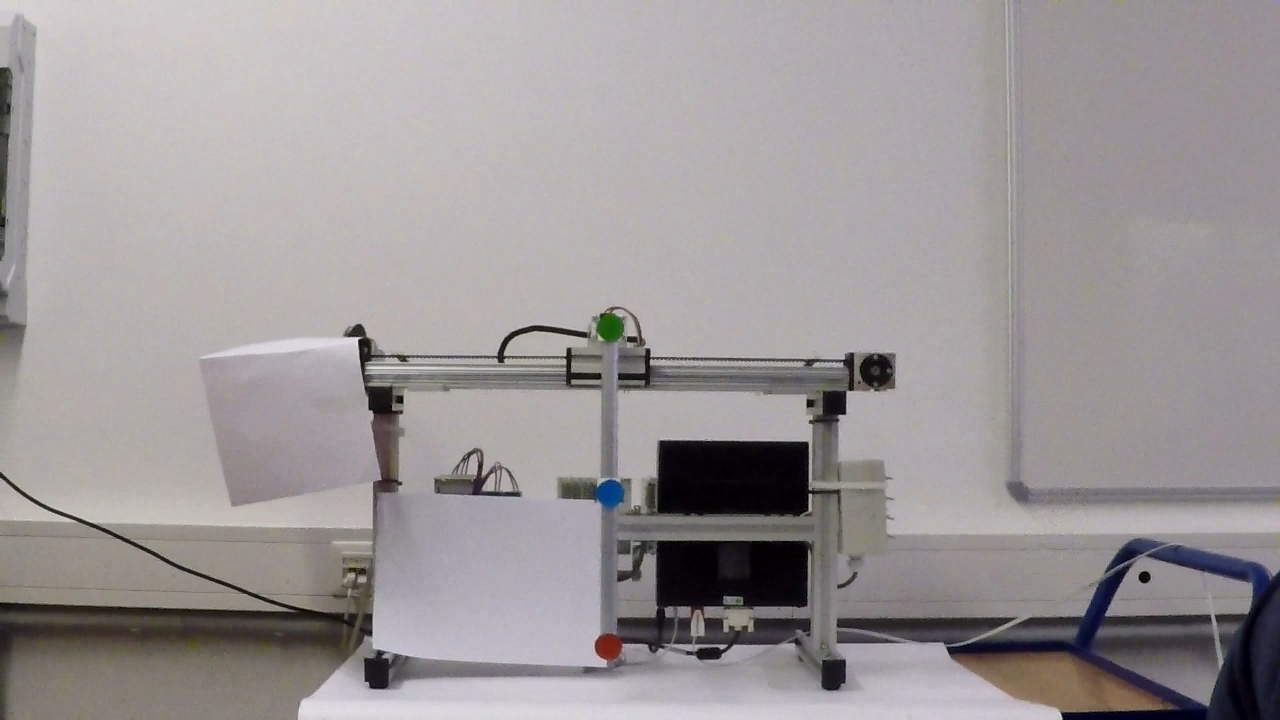
\includegraphics[width=0.7\textwidth]{imsubtract.png}%
	}%
	\centerline{%
		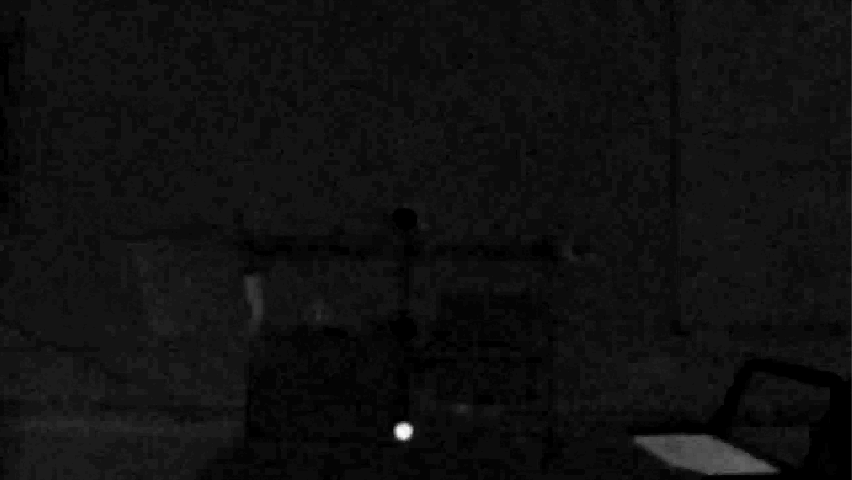
\includegraphics[width=0.7\textwidth]{imsubtractbintest.png}%
	}%
	\caption[Einzelbild des Doppelpendels vor und nach der Farbsegmentierung]{Einzelbild des Doppelpendels: RGB-Rohbild (oben), Graustufenbild nach Anwendung von~\eqref{eq:imsubtract} (unten)}
	\label{fig:imsubtractbild}
\end{figure}

F�r die Aufnahmen des Doppelpendels wird versucht, St�reinfl�sse bei der Farbsegmentierung zu vermeiden. Es tauchen neben den Markern kaum farbige Objekte auf. Das Doppelpendel wird vor eine wei�e Wand gestellt. Au�erdem werden farbige Kabel oder die braune Tischoberfl�che mit wei�em Papier verdeckt, um diese nicht f�lschlicherweise als farbige Objekte zu ermitteln. Dies erleichtert die Identifikation der Marker bei der Farbsegmentierung. Zus�tzlich werden die Pixelintensit�ten von Objekten, die nicht mit dem Arbeitsraum des Doppelpendels kollidieren, manuell auf Null gesetzt. Dieses Vorgehen wird f�r den blauen Griff des verfahrbaren Tischs in Bild~\ref{fig:imsubtractbild} angewendet. Ein weiterer St�rfaktor k�nnte durch eine Verdeckung des gr�nen Farbmarkers durch den �u�eren Pendelstab hervorgerufen werden. Da jedoch der innere Pendelstab l�nger als der �u�ere ist, kommt es nicht zu diesem Fall. Der gr�ne Marker wird zu jedem Zeitpunkt erkannt.

Auf das Graustufenbild wird ein nichtlineares $ (3\times 3)$-Medianfilter angewendet, um das Bild zu gl�tten und sogenannte \textit{Ausrei�erpixel} zu eliminieren. In der definierten Umgebung des untersuchten Pixels werden die Grauwerte der Gr��e nach sortiert und der mittlere Intensit�tswert f�r das Pixel eingesetzt. Damit wird sichergestellt, dass die Marker als zusammenh�ngendes Objekt erkannt werden und Pixel mit deutlich zu hohen oder geringen Intensit�tswerten nicht ber�cksichtigt werden. Im letzten Schritt der Farbsegmentierung wird das gefilterte Graustufenbild in eine bin�re Maske des roten Farbkanals
%
\begin{align}
	\bm{SW}^\mathrm{r}_{ij} = \begin{cases}
		1 & \text{f�r } \Delta \bm{B}^\mathrm{r}_{ij} \geq I_\mathrm{r} \\
		0 & \text{f�r } \Delta \bm{B}^\mathrm{r}_{ij} < I_\mathrm{r} 
	\end{cases}
	\label{eq:maskbin}
\end{align}

�berf�hrt mit $ \bm{SW}^\mathrm{r}_{ij} \in \mathds{R}^{(h\times b)}$. Es werden alle Eintr�ge der Maske, die gleich oder gr��er als der Schwellwert f�r die rote Farbintensit�t $ I_\mathrm{r} $ sind, auf 1 und die restlichen Werte auf 0 gesetzt. Der Schwellwert wird so eingestellt, dass neben dem farbigen Marker keine weiteren Objekte in der bin�ren Maske auftauchen. Die Ermittlung der bin�ren Masken $ \bm{SW}^\mathrm{g} $ und $ \bm{SW}^{\mathrm{b}} $ f�r den gr�nen und blauen Farbkanal werden analog unter Anwendung von~\eqref{eq:imsubtract}, des $ (3\times 3) $-Medianfilters und~\eqref{eq:maskbin} mit den Matrizen $ \bm{B}^\mathrm{g} $, $ \bm{B}^{\mathrm{b}} $ bestimmt. F�r die Berechnung des Objektschwerpunkts wird die Fl�che des Objekts
%
\begin{align}
	A = \sum_{i = 1}^{h} \left(\sum_{j=1}^{b} \bm{SW}_{ij}\right)
\end{align}

ermittelt. Trotz geschickter Wahl des Schwellwerts $ I $ bei der Bildung der bin�ren Maske in~\eqref{eq:maskbin} k�nnen Pixel, die nicht zum Farbmarker geh�ren, f�lschlicherweise in dem Bin�rbild auftauchen. Aus diesem Grund werden alle Objekte, die eine Mindestfl�che $ A_{\mathrm{min}} $ unterschreiten, nicht beachtet. In den Bin�rmasken taucht nun genau ein zusammenh�ngendes Objekt auf, welches dem farblichen Marker entspricht. Die Schwerpunktkoordinaten $ u_\mathrm{S} $ und $ v_\mathrm{S} $ im Bildkoordinatensystem $ KS_\mathrm{B} $ eines detektierten Markers in der Bin�rmaske ergeben sich damit zu
%
\begin{align}
	u_\mathrm{S} &= \frac{1}{A} \sum_{i=1}^{h} \left(  i \sum_{j=1}^{b}\bm{SW}_{\mathrm{ij}}\right), \label{eq:us} \\
	v_\mathrm{S} &= \frac{1}{A} \sum_{j=1}^{b} \left(  j \sum_{i=1}^{h} \bm{SW}_{ij} \right).
	\label{eq:vs}
\end{align}

Die Schwerpunkte $ \bm{c}_\mathrm{r} $, $ \bm{c}_\mathrm{g} $ und $ \bm{c}_\mathrm{b} $ der Marker werden mit~\eqref{eq:us} und~\eqref{eq:vs} bestimmt. Damit sind alle notwendigen Schritte f�r die Winkelberechnung gem��~\eqref{eq:phi} get�tigt. In Bild~\ref{fig:winkelmontage} ist ein Einzelbild des Doppelpendels vor und nach der Bildverarbeitung zu sehen. 
\begin{figure}[!htb]
	\centerline{%
		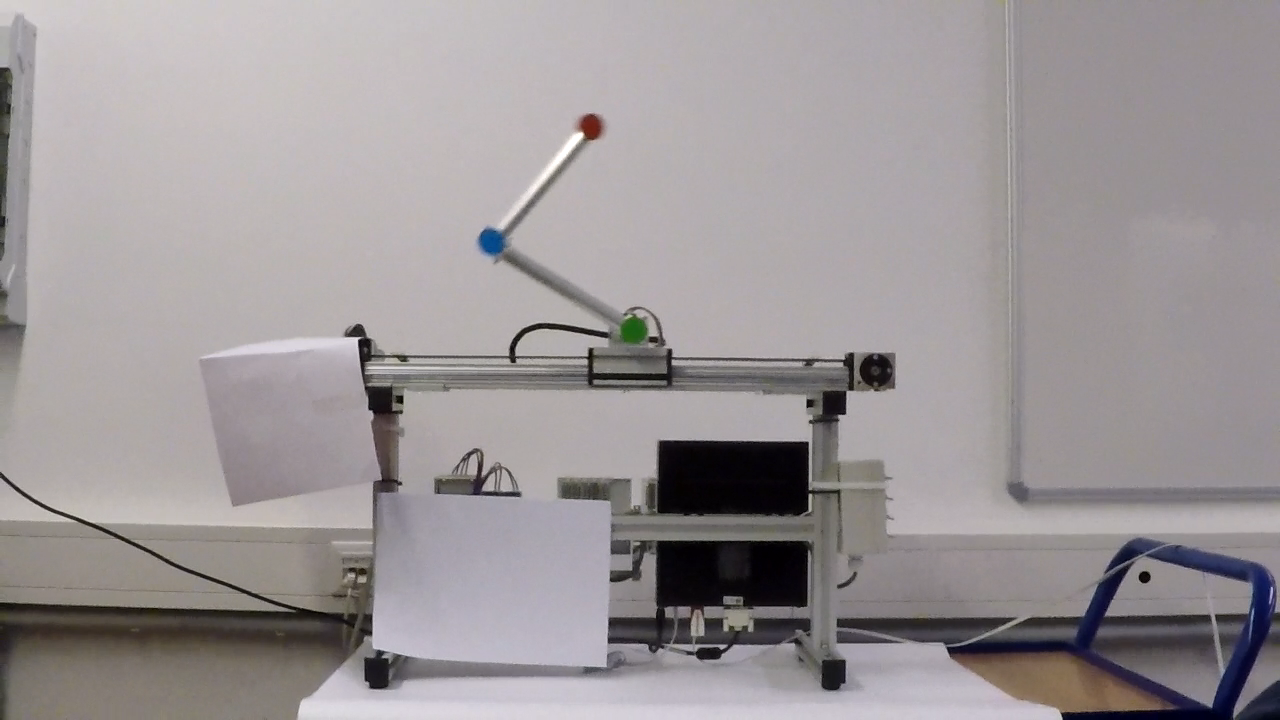
\includegraphics[width=0.7\textwidth]{dp.png}%
	}%
	\centerline{%
		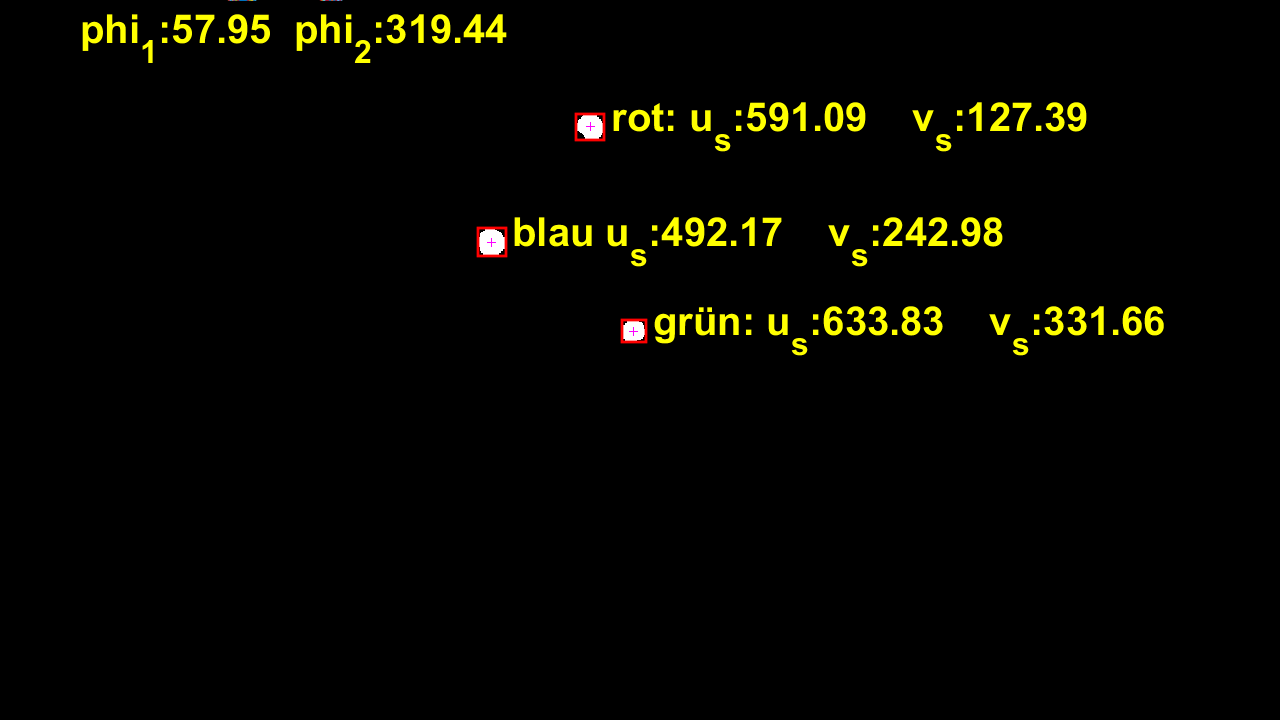
\includegraphics[width=0.7\textwidth]{bindptest.png}%
	}%
	\caption[Einzelbild des Doppelpendels vor und nach der Bildverarbeitung]{Einzelbild des Doppelpendels: RGB-Rohbild (oben), Bin�rmasken der drei Farbkan�le mit berechneten Winkeln $ \varphi_{1,\mathrm{B}} $ und $ \varphi_{2,\mathrm{B}} $ (unten)}
	\label{fig:winkelmontage}
\end{figure}

Es sind im unteren Bild die Schwerpunktkoordinaten der einzelnen Objekte und die berechneten Winkel $ \varphi_{1,\mathrm{B}} $ und $ \varphi_{2,\mathrm{B}} $ zu sehen. Um die bildbasierte Winkelbestimmung f�r die Validierung der Zustandssch�tzung durch das EKF verwenden zu k�nnen, wird diese zun�chst anhand einer Messung des inneren Pendelwinkels $ \varphi_1 $ �berpr�ft. 

\section{Validierung der bildbasierten Winkelbestimmung}
\label{sec:validierungwinkelbestimmung}

Der bildbasierte innere Pendelwinkel $ \varphi_{1,\mathrm{B}} $ wird anhand der Messung des Winkelsensors $ \varphi_1 $ validiert. Die Signale $ \varphi_1 $ und $ \varphi_{1,\mathrm{B}} $ weisen unterschiedliche Merkmale auf. Sie besitzen zum einen unterschiedliche Abtastraten, wie in Abschnitt~\ref{sec:bildbasiertewinkelmessung} erl�utert. Zum anderen weisen die Signale abweichende Startzeitpunkte und Zeitspannen auf, da es nicht m�glich ist, die Messungen der Wagenposition $ x $ und des Winkels $ \varphi_1$ und die Kameraufnahmen synchron zu starten und zu beenden.  Um die Winkelsignale miteinander zu vergleichen, wird das Kamerasignal $ \varphi_{1,\mathrm{B}}$ mit einer Bildfrequenz von \SI{240}{fps} mit der Abtastrate des mechatronischen Systems von \SI{1000}{\hertz} erneut abgetastet und interpoliert. Im Anschluss wird eine Kreuzkorrelation von $ \varphi_1 $ und $ \varphi_{1,\mathrm{B}} $ vorgenommen, um den Zeitversatz beider Signale zu ermitteln. Danach k�nnen beide Signale mit dem gleichen Startzeitpunkt ausgerichtet werden. Die einzelnen Schritte der erneuten Abtastung und Kreuzkorrelation werden an dieser Stelle nicht im Detail erl�utert. In Bild~\ref{fig:validierungphi1} sind die gleichgerichteten Winkel f�r einen Ausschwingversuch des Doppelpendels zu sehen. Der Anfangszustand lautet in diesem Fall:
%
\begin{align*}
	\bm{x}_0 = \Big[ \varphi_{1,0} = \ang{90}, \dot{\varphi}_{1,0} = 0, \varphi_{2,0} = 0, \dot{\varphi}_{2,0} = 180 \Big]^{\mathrm{T}}.
\end{align*}


\begin{figure}[!htb]
	\centering
	% This file was created by matlab2tikz.
%
%The latest updates can be retrieved from
%  http://www.mathworks.com/matlabcentral/fileexchange/22022-matlab2tikz-matlab2tikz
%where you can also make suggestions and rate matlab2tikz.
%
\begin{tikzpicture}

\begin{axis}[%
width=4.521in,
height=3.566in,
at={(0.758in,0.481in)},
scale only axis,
xmin=0,
xmax=10,
xlabel style={font=\color{white!15!black}},
xlabel={Zeit [s]},
ymin=80,
ymax=260,
ylabel style={font=\color{white!15!black}},
ylabel={Winkel [Grad]},
axis background/.style={fill=white},
xmajorgrids,
ymajorgrids,
grid style={dotted},
legend style={legend cell align=left, align=left, draw=white!15!black}
]
\addplot [color=red]
  table[row sep=crcr]{%
0	87.283190187169\\
0.01	88.3084253656626\\
0.02	89.5962176493577\\
0.03	91.2455166208564\\
0.04	93.0563913299375\\
0.05	95.4359071802058\\
0.06	98.045420817512\\
0.07	100.839015275592\\
0.08	104.269598872119\\
0.09	107.793250905191\\
0.1	111.767267556203\\
0.11	116.103257628551\\
0.12	121.060914611629\\
0.13	126.442860256855\\
0.14	132.113932629694\\
0.15	138.043986837156\\
0.16	144.435756239897\\
0.17	151.145761031101\\
0.18	158.09728239299\\
0.19	164.495877592612\\
0.2	170.90858689817\\
0.21	177.112149637761\\
0.22	182.980828184671\\
0.23	188.854998453919\\
0.24	194.682120622189\\
0.25	200.124775614594\\
0.26	205.247693160593\\
0.27	209.864360166571\\
0.28	214.528710284393\\
0.29	218.017294665713\\
0.3	221.685389518079\\
0.31	224.772480386325\\
0.32	227.249453940515\\
0.33	229.406339369864\\
0.34	230.575048101844\\
0.35	231.396125701806\\
0.36	231.644169030786\\
0.37	231.085754836151\\
0.38	230.68543398623\\
0.39	229.569428300745\\
0.4	229.023534495034\\
0.41	228.62717821956\\
0.42	228.348636022004\\
0.43	228.37495631701\\
0.44	228.284919459291\\
0.45	228.292228233223\\
0.46	228.633001121715\\
0.47	228.650332626706\\
0.48	228.942596453359\\
0.49	228.90959893393\\
0.5	228.929425806253\\
0.51	228.899411174815\\
0.52	228.629597340806\\
0.53	228.440999644268\\
0.54	227.886542801997\\
0.55	227.261338647413\\
0.56	226.792547032319\\
0.57	226.24433406201\\
0.58	224.391714468204\\
0.59	222.78920313176\\
0.6	221.196566486953\\
0.61	219.252036236263\\
0.62	217.205157213867\\
0.63	214.899426755602\\
0.64	212.057720374622\\
0.65	209.327649081956\\
0.66	206.120586922916\\
0.67	202.622410336461\\
0.68	198.754922541245\\
0.69	194.105855072338\\
0.7	188.540098146048\\
0.71	182.858704356367\\
0.72	176.060466047866\\
0.73	169.487097494774\\
0.74	163.21368289579\\
0.75	157.624373337568\\
0.76	152.940539818609\\
0.77	148.37436978212\\
0.78	144.924776641486\\
0.79	141.730054273799\\
0.8	139.00248366129\\
0.81	136.859586539855\\
0.82	134.795610631127\\
0.83	133.232806182636\\
0.84	131.833310894814\\
0.85	130.634261563976\\
0.86	130.062165122499\\
0.87	130.043386354776\\
0.88	129.197093293444\\
0.89	128.931943217583\\
0.9	129.632901473452\\
0.91	130.258844310209\\
0.92	130.80657580541\\
0.93	131.801512242728\\
0.94	132.75827156466\\
0.95	133.84923193547\\
0.96	135.212877291399\\
0.97	136.522282296001\\
0.98	137.988297737138\\
0.99	139.254956816874\\
1	140.741719993424\\
1.01	142.24448299555\\
1.02	143.396553863939\\
1.03	144.748162091794\\
1.04	145.858584631906\\
1.05	146.777131553544\\
1.06	147.511373229116\\
1.07	147.684045156074\\
1.08	147.704721468721\\
1.09	147.258884322727\\
1.1	146.750964371703\\
1.11	146.487950469602\\
1.12	146.308794243548\\
1.13	146.815062173612\\
1.14	147.841031392321\\
1.15	149.277135905108\\
1.16	151.827840449321\\
1.17	154.656486008792\\
1.18	157.692265442277\\
1.19	161.435668516707\\
1.2	165.394682711798\\
1.21	169.636374417475\\
1.22	173.932804979416\\
1.23	178.554075583969\\
1.24	183.108591392024\\
1.25	187.786433175614\\
1.26	192.781860794091\\
1.27	197.333380546618\\
1.28	201.790033859712\\
1.29	206.539162867381\\
1.3	210.976206317473\\
1.31	215.790530987191\\
1.32	220.23753045449\\
1.33	224.909674907346\\
1.34	229.29313150736\\
1.35	233.419781715422\\
1.36	237.471243074778\\
1.37	240.833137364936\\
1.38	244.021450547241\\
1.39	247.033786639525\\
1.4	248.953177624009\\
1.41	251.036523751411\\
1.42	252.480001728916\\
1.43	253.895647840733\\
1.44	254.766571290402\\
1.45	255.351620240139\\
1.46	255.678699206423\\
1.47	255.286018973789\\
1.48	254.965371707504\\
1.49	254.267001277319\\
1.5	252.980113380634\\
1.51	251.591606252874\\
1.52	249.744275017372\\
1.53	247.79021487922\\
1.54	245.592508690045\\
1.55	242.688151600152\\
1.56	239.761444839149\\
1.57	236.285458927032\\
1.58	232.650711153171\\
1.59	228.896800096263\\
1.6	224.467380235108\\
1.61	220.228097553297\\
1.62	215.240953361688\\
1.63	209.684054239255\\
1.64	204.058764362506\\
1.65	197.988224013439\\
1.66	191.621170021152\\
1.67	185.436899421301\\
1.68	179.985898970184\\
1.69	174.233957519188\\
1.7	168.764018789407\\
1.71	163.865479407238\\
1.72	158.850274696086\\
1.73	154.13387090227\\
1.74	149.712068446543\\
1.75	145.325213548968\\
1.76	141.525989886768\\
1.77	137.759446684753\\
1.78	134.287507725524\\
1.79	131.480400477676\\
1.8	128.981632459771\\
1.81	126.689537836113\\
1.82	125.124718838093\\
1.83	123.812484568644\\
1.84	123.310670977981\\
1.85	122.933813907823\\
1.86	123.155582722873\\
1.87	123.99703566612\\
1.88	125.059281329149\\
1.89	126.5712051145\\
1.9	128.139902167759\\
1.91	129.863888309398\\
1.92	131.513392689527\\
1.93	133.082279760255\\
1.94	134.840177124024\\
1.95	136.391518215303\\
1.96	137.982411225053\\
1.97	139.590658657419\\
1.98	141.074707277944\\
1.99	143.22514628173\\
2	145.032122919826\\
2.01	147.084507055387\\
2.02	149.421668468393\\
2.03	151.777111604893\\
2.04	154.587836980176\\
2.05	157.142014362943\\
2.06	160.08651050662\\
2.07	163.429104445967\\
2.08	166.736821609801\\
2.09	170.335001949286\\
2.1	173.80221756017\\
2.11	177.484162441528\\
2.12	181.390388505472\\
2.13	184.920953560033\\
2.14	189.29783146374\\
2.15	193.474734042812\\
2.16	197.511065234474\\
2.17	201.365687075293\\
2.18	205.066501272825\\
2.19	208.811030932071\\
2.2	212.293631926164\\
2.21	215.55496974502\\
2.22	218.535167122139\\
2.23	221.448218359511\\
2.24	224.246691007072\\
2.25	226.2153587142\\
2.26	228.09156233183\\
2.27	229.48332699253\\
2.28	230.53025319476\\
2.29	231.452581628461\\
2.3	231.23011390426\\
2.31	230.915454626626\\
2.32	229.964449008014\\
2.33	228.288654185183\\
2.34	226.303323023941\\
2.35	223.235463447415\\
2.36	220.060260986018\\
2.37	215.924861004562\\
2.38	211.566804578394\\
2.39	207.533440614641\\
2.4	203.535073641498\\
2.41	200.042031396109\\
2.42	197.076673984099\\
2.43	194.036238473564\\
2.44	191.262368505113\\
2.45	188.540499605749\\
2.46	185.695094174067\\
2.47	183.342888321768\\
2.48	180.790118868022\\
2.49	178.441470035255\\
2.5	175.859283726386\\
2.51	173.394406175432\\
2.52	170.99740143571\\
2.53	168.417647361998\\
2.54	166.032867144664\\
2.55	163.449955259876\\
2.56	160.81088715741\\
2.57	159.273850874412\\
2.58	155.971134368365\\
2.59	154.066584575454\\
2.6	151.195847378253\\
2.61	150.413554102202\\
2.62	148.862931804634\\
2.63	147.114116752057\\
2.64	145.941449373064\\
2.65	144.908863044739\\
2.66	144.031386398647\\
2.67	143.552272714431\\
2.68	143.065202968269\\
2.69	142.970287863926\\
2.7	142.823581703678\\
2.71	143.063266538913\\
2.72	143.562989783303\\
2.73	143.974459840797\\
2.74	144.65102129633\\
2.75	145.477680034967\\
2.76	146.330863466142\\
2.77	147.473759700276\\
2.78	148.542353726914\\
2.79	149.907382768396\\
2.8	150.975752396553\\
2.81	152.205430320577\\
2.82	153.367153188681\\
2.83	154.161140215226\\
2.84	155.196627577406\\
2.85	155.72350260559\\
2.86	156.113264482826\\
2.87	156.332424021177\\
2.88	155.994011705945\\
2.89	155.630398223911\\
2.9	155.105845933398\\
2.91	154.590144733421\\
2.92	154.668733767015\\
2.93	154.936570426265\\
2.94	155.991904959382\\
2.95	157.445429526318\\
2.96	159.195255370291\\
2.97	161.584527997017\\
2.98	164.137705404449\\
2.99	166.915470158603\\
3	170.143681221297\\
3.01	173.444043089648\\
3.02	177.21013831598\\
3.03	180.892804079065\\
3.04	184.626873990467\\
3.05	188.522590718435\\
3.06	192.236169662373\\
3.07	196.28661040247\\
3.08	199.797142138466\\
3.09	203.315346238842\\
3.1	207.001665577911\\
3.11	210.587988817196\\
3.12	214.326244594234\\
3.13	217.757314001857\\
3.14	221.21599114554\\
3.15	224.720566421324\\
3.16	227.814922207673\\
3.17	231.003065514137\\
3.18	233.586228323714\\
3.19	235.929470933606\\
3.2	238.276142339441\\
3.21	239.941608891822\\
3.22	241.44272497995\\
3.23	242.14274767246\\
3.24	242.821841384341\\
3.25	243.239942388207\\
3.26	243.071299502626\\
3.27	242.842694783364\\
3.28	242.092850629952\\
3.29	241.035892430252\\
3.3	239.838595737737\\
3.31	238.020568194907\\
3.32	236.255203243962\\
3.33	233.859186200283\\
3.34	231.405971205171\\
3.35	228.676833881119\\
3.36	225.236871196834\\
3.37	221.957141958033\\
3.38	218.255942626208\\
3.39	214.046156192854\\
3.4	209.718778723132\\
3.41	204.797397932288\\
3.42	199.995211387597\\
3.43	194.924125164291\\
3.44	189.702897638546\\
3.45	184.682744416857\\
3.46	179.50340157276\\
3.47	174.747933810203\\
3.48	170.075604918886\\
3.49	165.615509422297\\
3.5	161.609473741829\\
3.51	157.357025256885\\
3.52	153.641810642175\\
3.53	150.084972847273\\
3.54	146.563331244165\\
3.55	143.949029159053\\
3.56	141.129323877071\\
3.57	138.921741626951\\
3.58	137.038522753005\\
3.59	135.323307569385\\
3.6	134.269547290854\\
3.61	133.393002793151\\
3.62	132.955156727455\\
3.63	132.924213099621\\
3.64	133.358624710887\\
3.65	133.856553747373\\
3.66	134.605027419511\\
3.67	135.666095380394\\
3.68	136.855968064949\\
3.69	137.951111718514\\
3.7	139.134629290831\\
3.71	140.271723912718\\
3.72	141.481135708322\\
3.73	142.780536180363\\
3.74	143.989375998716\\
3.75	145.393427593213\\
3.76	146.762749688708\\
3.77	148.343933993103\\
3.78	150.062959858722\\
3.79	151.802938839991\\
3.8	153.956217761624\\
3.81	155.890144406072\\
3.82	158.156210814066\\
3.83	160.490509319396\\
3.84	162.948296048332\\
3.85	165.783891680005\\
3.86	168.295444648762\\
3.87	171.261993679785\\
3.88	174.17315822023\\
3.89	177.118263088283\\
3.9	180.390478386045\\
3.91	183.155294130988\\
3.92	186.21019153997\\
3.93	189.372876629973\\
3.94	191.960448822763\\
3.95	195.021828548102\\
3.96	197.103995439055\\
3.97	199.218332779044\\
3.98	201.194332099961\\
3.99	202.085613845004\\
4	203.083763704654\\
4.01	203.153675693684\\
4.02	202.902897936658\\
4.03	202.390035549527\\
4.04	200.912593480349\\
4.05	199.228630558618\\
4.06	197.046722515786\\
4.07	195.061176666014\\
4.08	193.363642321751\\
4.09	191.698260471844\\
4.1	190.781998171125\\
4.11	190.218587797802\\
4.12	189.836585668436\\
4.13	189.973566358982\\
4.14	190.014985666781\\
4.15	190.331469580814\\
4.16	190.746155683886\\
4.17	191.29889037138\\
4.18	192.062954797974\\
4.19	192.57585559647\\
4.2	193.307885284693\\
4.21	193.936978530635\\
4.22	194.32498858027\\
4.23	194.904439691072\\
4.24	195.190449075301\\
4.25	195.47032428245\\
4.26	195.69085644308\\
4.27	195.716412343576\\
4.28	195.92490340311\\
4.29	195.575137300404\\
4.3	195.419661555192\\
4.31	195.505485713561\\
4.32	194.869198679641\\
4.33	194.10771094978\\
4.34	192.889756648446\\
4.35	192.513504747124\\
4.36	191.940721214812\\
4.37	191.212257376166\\
4.38	190.444863611653\\
4.39	189.547469003615\\
4.4	188.750838818218\\
4.41	187.671195756166\\
4.42	186.791297239398\\
4.43	185.960245225801\\
4.44	184.760253021541\\
4.45	183.846191993541\\
4.46	182.823784558078\\
4.47	181.501455042396\\
4.48	180.250541222063\\
4.49	178.750108610139\\
4.5	177.160098561403\\
4.51	175.359193555684\\
4.52	173.342050205509\\
4.53	171.236865724806\\
4.54	168.183694218364\\
4.55	165.248791823984\\
4.56	161.801010761073\\
4.57	158.348250898315\\
4.58	155.226511332114\\
4.59	152.193069535448\\
4.6	149.86520243494\\
4.61	148.091621032847\\
4.62	146.717663071188\\
4.63	145.899816352848\\
4.64	145.406803722403\\
4.65	145.358465433688\\
4.66	145.76599637969\\
4.67	146.378250207772\\
4.68	147.583247886168\\
4.69	148.770512330449\\
4.7	150.433825660834\\
4.71	152.361428523008\\
4.72	154.241634462988\\
4.73	156.435589915289\\
4.74	158.569856205578\\
4.75	161.030367206041\\
4.76	163.496072336123\\
4.77	165.604877317969\\
4.78	168.144323793953\\
4.79	170.495425066218\\
4.8	172.975331688507\\
4.81	175.518563632706\\
4.82	177.71250729511\\
4.83	180.036165355587\\
4.84	182.176777818501\\
4.85	184.490376781029\\
4.86	186.656672448114\\
4.87	188.632417923917\\
4.88	190.84489726947\\
4.89	193.026475069545\\
4.9	195.101760927949\\
4.91	197.430215002456\\
4.92	199.398872551964\\
4.93	201.982679337149\\
4.94	204.293747343066\\
4.95	206.70399483896\\
4.96	209.42749562601\\
4.97	212.211536549715\\
4.98	214.928785109779\\
4.99	217.231971582215\\
5	219.465446176981\\
5.01	221.177917197095\\
5.02	222.260846169748\\
5.03	223.185164164117\\
5.04	223.517616349648\\
5.05	223.50959260741\\
5.06	223.267235026513\\
5.07	222.470607130231\\
5.08	221.648616229106\\
5.09	220.183427004063\\
5.1	218.527840560635\\
5.11	216.939358960648\\
5.12	214.597799070341\\
5.13	212.318756205371\\
5.14	209.74469925999\\
5.15	206.97624040472\\
5.16	204.238575653953\\
5.17	201.004652699082\\
5.18	197.954109165711\\
5.19	194.341796557773\\
5.2	190.682805466656\\
5.21	187.141337421364\\
5.22	183.145618940785\\
5.23	179.352634092641\\
5.24	175.140858221694\\
5.25	170.908658086049\\
5.26	166.577416842675\\
5.27	161.909059401394\\
5.28	157.557298360871\\
5.29	153.310220887218\\
5.3	149.380646428539\\
5.31	145.965142268627\\
5.32	142.611015822057\\
5.33	139.836905427771\\
5.34	137.189667576834\\
5.35	134.873044141218\\
5.36	133.297962036036\\
5.37	131.489678033441\\
5.38	130.09819991333\\
5.39	129.093044629949\\
5.4	128.245853102679\\
5.41	127.694948150058\\
5.42	127.410933878594\\
5.43	127.408654368005\\
5.44	127.536838472773\\
5.45	127.946151800326\\
5.46	128.669361704363\\
5.47	129.553761591285\\
5.48	130.89416780977\\
5.49	132.359865318892\\
5.5	133.990800440923\\
5.51	136.15110375231\\
5.52	138.20984632063\\
5.53	140.757774875805\\
5.54	143.676181250558\\
5.55	146.862798122447\\
5.56	150.493140901607\\
5.57	154.286277461765\\
5.58	158.587727316746\\
5.59	163.028644422947\\
5.6	167.418824036093\\
5.61	172.083946775603\\
5.62	176.447658416431\\
5.63	180.842318246536\\
5.64	184.754727558488\\
5.65	188.634272091586\\
5.66	192.253721856397\\
5.67	195.911465322803\\
5.68	199.338436219976\\
5.69	202.45098121218\\
5.7	205.296187439777\\
5.71	208.173677799068\\
5.72	210.596621646008\\
5.73	212.948771746285\\
5.74	215.209106275213\\
5.75	216.849518534813\\
5.76	218.743988051255\\
5.77	220.036995085401\\
5.78	221.156969219554\\
5.79	222.217733281752\\
5.8	222.690841307666\\
5.81	223.168684445016\\
5.82	222.927820836963\\
5.83	222.531598352393\\
5.84	221.954137621515\\
5.85	220.505437998063\\
5.86	219.148783469904\\
5.87	217.289521274398\\
5.88	214.833972789873\\
5.89	212.281533718036\\
5.9	209.725084497926\\
5.91	206.871689283018\\
5.92	204.205806278908\\
5.93	201.705861524017\\
5.94	199.241608579447\\
5.95	196.878258298075\\
5.96	194.661727765517\\
5.97	192.276404252888\\
5.98	190.070432894229\\
5.99	188.113426143354\\
6	185.539486992528\\
6.01	183.364825904273\\
6.02	181.096322410889\\
6.03	178.941161599161\\
6.04	176.726264226954\\
6.05	174.368081330545\\
6.06	172.109837718838\\
6.07	169.631678611545\\
6.08	167.422212956648\\
6.09	165.483698624146\\
6.1	163.217606566275\\
6.11	161.26011573258\\
6.12	159.379623106664\\
6.13	157.574113483837\\
6.14	156.382769632887\\
6.15	155.00456927223\\
6.16	154.053668520328\\
6.17	153.341633249611\\
6.18	152.861995232646\\
6.19	153.04217624622\\
6.2	153.236591351574\\
6.21	154.195192325512\\
6.22	155.616137844454\\
6.23	157.371172760085\\
6.24	159.520053110932\\
6.25	161.706473310889\\
6.26	164.317654037032\\
6.27	166.713965717238\\
6.28	168.891109073407\\
6.29	170.797843912899\\
6.3	172.378698455641\\
6.31	173.688264018151\\
6.32	174.776256899292\\
6.33	175.610062020676\\
6.34	176.641250714428\\
6.35	177.2153490734\\
6.36	178.061143837\\
6.37	178.589860355216\\
6.38	179.133751425184\\
6.39	179.741876789606\\
6.4	180.268652840514\\
6.41	180.861586425311\\
6.42	181.451031021105\\
6.43	182.003357328375\\
6.44	182.751696878472\\
6.45	183.289765521913\\
6.46	184.077681589881\\
6.47	184.858225610631\\
6.48	185.610022398584\\
6.49	186.602455452072\\
6.5	187.400074135517\\
6.51	188.405197220951\\
6.52	189.274006394952\\
6.53	190.022730397479\\
6.54	191.219368368924\\
6.55	192.025828595881\\
6.56	192.853189826944\\
6.57	193.64691281858\\
6.58	194.216282173122\\
6.59	194.863882204899\\
6.6	195.2061007118\\
6.61	195.606029475429\\
6.62	195.971684699456\\
6.63	195.874166512157\\
6.64	195.644279893739\\
6.65	195.116823612822\\
6.66	194.3738574524\\
6.67	193.668389093491\\
6.68	191.980924609758\\
6.69	190.21531054708\\
6.7	187.832036078117\\
6.71	185.206327089709\\
6.72	182.463806313213\\
6.73	179.377805417629\\
6.74	176.524747410128\\
6.75	173.732433663752\\
6.76	171.496295116655\\
6.77	169.841932393013\\
6.78	168.163338229791\\
6.79	167.306498805902\\
6.8	166.329635559052\\
6.81	165.691806650072\\
6.82	165.397825120445\\
6.83	165.055409652715\\
6.84	165.161455086127\\
6.85	165.227947601435\\
6.86	165.519359017159\\
6.87	165.944583987895\\
6.88	166.208868267833\\
6.89	166.791991764753\\
6.9	167.297891219811\\
6.91	167.891035822159\\
6.92	168.564858786483\\
6.93	169.008006268828\\
6.94	169.797876463345\\
6.95	170.313869714602\\
6.96	170.931604894846\\
6.97	171.743401125693\\
6.98	172.180893564252\\
6.99	172.959908221964\\
7	173.432650886174\\
7.01	173.88287332546\\
7.02	174.671542073175\\
7.03	175.135234721857\\
7.04	175.813644243109\\
7.05	176.436785787855\\
7.06	177.075799832333\\
7.07	177.987873708191\\
7.08	178.564789786248\\
7.09	179.508923192428\\
7.1	180.655814375489\\
7.11	181.866941097538\\
7.12	183.357917712863\\
7.13	184.876718138131\\
7.14	186.683588645704\\
7.15	188.837417454611\\
7.16	191.154192854636\\
7.17	194.034245845529\\
7.18	196.558663446638\\
7.19	198.991567791223\\
7.2	201.113565463076\\
7.21	202.596869018939\\
7.22	203.935225017814\\
7.23	204.698671072484\\
7.24	205.21577270602\\
7.25	205.54602543873\\
7.26	205.374368477003\\
7.27	205.034075185892\\
7.28	204.206550142339\\
7.29	203.353567700046\\
7.3	202.216709012129\\
7.31	200.88445678889\\
7.32	199.604370920186\\
7.33	198.15250581517\\
7.34	196.349873989625\\
7.35	194.799505993019\\
7.36	192.921885453546\\
7.37	191.251913227081\\
7.38	189.044149909901\\
7.39	187.100483177908\\
7.4	185.272766120306\\
7.41	183.185406027325\\
7.42	181.275835549904\\
7.43	179.157398592181\\
7.44	176.911473847009\\
7.45	174.81127849307\\
7.46	172.467428063342\\
7.47	170.232886345371\\
7.48	167.586124902191\\
7.49	164.951644433691\\
7.5	162.266273337662\\
7.51	159.419136774949\\
7.52	156.604538661936\\
7.53	153.782497980173\\
7.54	151.356871353486\\
7.55	149.112643751513\\
7.56	147.057199419227\\
7.57	145.467032531477\\
7.58	144.153615673869\\
7.59	143.215511745122\\
7.6	142.763636746143\\
7.61	142.340546830066\\
7.62	142.547401499624\\
7.63	142.768758312916\\
7.64	143.335673823803\\
7.65	144.211482827261\\
7.66	145.122718255436\\
7.67	146.258413568759\\
7.68	147.708173854924\\
7.69	149.288357100046\\
7.7	151.21254458912\\
7.71	153.136605486947\\
7.72	155.41501041976\\
7.73	157.735520120029\\
7.74	160.111109777615\\
7.75	162.921837206739\\
7.76	165.730996494113\\
7.77	168.8061562149\\
7.78	172.011474542888\\
7.79	175.260149407123\\
7.8	179.03402535632\\
7.81	182.513180005662\\
7.82	186.351369020536\\
7.83	190.427310963034\\
7.84	194.324442127695\\
7.85	198.26320707645\\
7.86	201.313770965094\\
7.87	204.442469615232\\
7.88	206.947654920456\\
7.89	209.286843711962\\
7.9	211.781094425236\\
7.91	213.4372144442\\
7.92	215.31707825284\\
7.93	216.615104967602\\
7.94	217.678658313099\\
7.95	218.957780214794\\
7.96	219.677492204627\\
7.97	220.283163328197\\
7.98	220.653769732717\\
7.99	220.529383692567\\
8	220.643647982763\\
8.01	220.321927337678\\
8.02	219.773267510588\\
8.03	219.005598274089\\
8.04	218.018636284093\\
8.05	216.900989626369\\
8.06	215.163664269729\\
8.07	213.433101162129\\
8.08	211.324635840374\\
8.09	208.595331130215\\
8.1	205.99565753908\\
8.11	202.88731605326\\
8.12	199.603404099656\\
8.13	196.461565295459\\
8.14	192.66528925535\\
8.15	189.278908846498\\
8.16	185.793681380405\\
8.17	182.67163688391\\
8.18	179.545117385425\\
8.19	176.563627506557\\
8.2	173.913546288084\\
8.21	171.245736226581\\
8.22	168.754041598295\\
8.23	166.353511983988\\
8.24	164.063777657164\\
8.25	162.071279989373\\
8.26	159.838028247123\\
8.27	157.939582255319\\
8.28	156.273439604897\\
8.29	154.542340964762\\
8.3	153.222164885206\\
8.31	152.061674580877\\
8.32	150.985608704803\\
8.33	150.340246045869\\
8.34	149.788000180129\\
8.35	149.619398309763\\
8.36	149.525820453408\\
8.37	149.842663410206\\
8.38	150.514961785589\\
8.39	151.506967307538\\
8.4	152.983398060552\\
8.41	154.611644346333\\
8.42	156.539302529006\\
8.43	158.764011465317\\
8.44	160.955213868207\\
8.45	163.236930042315\\
8.46	165.346038449166\\
8.47	167.383498422445\\
8.48	169.281213652504\\
8.49	170.936584080412\\
8.5	172.65235626106\\
8.51	174.050467756674\\
8.52	175.500858350368\\
8.53	177.082453237006\\
8.54	178.299783210068\\
8.55	179.602553859977\\
8.56	180.804427382959\\
8.57	182.089166813328\\
8.58	183.41206564006\\
8.59	184.405006901721\\
8.6	185.664997207872\\
8.61	186.964007940051\\
8.62	188.133182624836\\
8.63	189.436088934089\\
8.64	190.43259455464\\
8.65	191.442994938244\\
8.66	192.440832314973\\
8.67	193.350244031729\\
8.68	194.287583284928\\
8.69	194.688437109365\\
8.7	195.243437426537\\
8.71	195.43385378075\\
8.72	195.262326559652\\
8.73	194.99403649156\\
8.74	194.369034290402\\
8.75	193.452276470891\\
8.76	192.030063302646\\
8.77	190.417388015097\\
8.78	188.879140884144\\
8.79	186.437891388873\\
8.8	184.425227018151\\
8.81	182.467089181047\\
8.82	180.535438910172\\
8.83	179.209987232062\\
8.84	177.820804289254\\
8.85	176.741820995026\\
8.86	175.819716373256\\
8.87	175.201386089716\\
8.88	174.79474255218\\
8.89	174.409567825219\\
8.9	174.298495602074\\
8.91	174.272829141797\\
8.92	174.217354133986\\
8.93	174.405454866148\\
8.94	174.408273350039\\
8.95	174.485424835567\\
8.96	174.763308543364\\
8.97	174.881113234154\\
8.98	175.167354313412\\
8.99	175.343556474431\\
9	175.452232683158\\
9.01	175.686916303152\\
9.02	175.797736221462\\
9.03	176.207614927369\\
9.04	176.426751824702\\
9.05	176.729699684267\\
9.06	177.146927861233\\
9.07	177.451739584471\\
9.08	178.022447381812\\
9.09	178.4797487611\\
9.1	179.15988576561\\
9.11	180.145565543292\\
9.12	181.026075270248\\
9.13	182.255221247907\\
9.14	183.556960004576\\
9.15	184.989800280937\\
9.16	186.766099953883\\
9.17	188.530169077464\\
9.18	190.758627489004\\
9.19	192.648175727073\\
9.2	194.531428351587\\
9.21	196.083772834276\\
9.22	196.977251985133\\
9.23	198.005563072837\\
9.24	198.434631606771\\
9.25	198.742358756476\\
9.26	198.868557423602\\
9.27	198.391512056414\\
9.28	198.062657915524\\
9.29	197.375192447607\\
9.3	196.5863007097\\
9.31	195.857006696404\\
9.32	194.592331936767\\
9.33	193.401763482697\\
9.34	192.274033933028\\
9.35	190.506611952756\\
9.36	189.121800129147\\
9.37	187.481650677322\\
9.38	185.817777130927\\
9.39	184.360427337648\\
9.4	182.64212769622\\
9.41	180.982459252358\\
9.42	179.18127019585\\
9.43	177.384276726709\\
9.44	175.328364973818\\
9.45	173.049773237306\\
9.46	171.029765236903\\
9.47	168.698331852025\\
9.48	166.370681990422\\
9.49	163.863909362342\\
9.5	161.284841854258\\
9.51	159.062267625297\\
9.52	156.533199386939\\
9.53	154.541415385764\\
9.54	152.785150447491\\
9.55	151.275164761236\\
9.56	150.168504401538\\
9.57	149.188446832087\\
9.58	148.588740777671\\
9.59	148.199818709791\\
9.6	147.952658222265\\
9.61	148.26014364841\\
9.62	148.482277557044\\
9.63	149.127957215748\\
9.64	149.860992283935\\
9.65	150.823119918216\\
9.66	152.240325461885\\
9.67	153.483972071639\\
9.68	155.08062888578\\
9.69	156.855165834013\\
9.7	158.649557142299\\
9.71	160.850758534687\\
9.72	162.964917243285\\
9.73	165.38488290299\\
9.74	167.979646231556\\
9.75	170.705677755987\\
9.76	173.818341246724\\
9.77	176.816463361045\\
9.78	180.204325263346\\
9.79	183.441428921869\\
9.8	186.534815896738\\
9.81	190.088538980032\\
9.82	193.236336491721\\
9.83	196.139071972445\\
9.84	198.843655997825\\
9.85	201.229657954005\\
9.86	203.599948637081\\
9.87	205.390949289581\\
9.88	207.229399175406\\
9.89	208.704824590496\\
9.9	209.815399423957\\
9.91	211.16156471704\\
9.92	212.036184271521\\
9.93	212.867659075805\\
9.94	213.343968325253\\
9.95	213.407625907379\\
9.96	213.643693521468\\
9.97	213.361767695497\\
9.98	213.032950480738\\
9.99	212.50164766412\\
10	211.576399393275\\
};
\addlegendentry{Messung}

\addplot [color=blue]
  table[row sep=crcr]{%
0	86.674458536923\\
0.01	87.1691524862663\\
0.02	87.938676407467\\
0.03	89.4502412526828\\
0.04	90.7144591232269\\
0.05	92.7482009149717\\
0.06	95.0018066842025\\
0.07	97.282895450619\\
0.08	100.058678166379\\
0.09	102.834460882139\\
0.1	106.379767519099\\
0.11	109.92507415606\\
0.12	114.459768691707\\
0.13	118.747116252683\\
0.14	123.803987734859\\
0.15	129.355553166379\\
0.16	135.429295544428\\
0.17	141.228207950619\\
0.18	147.301950328668\\
0.19	154.117733630732\\
0.2	160.19147600878\\
0.21	167.007259310844\\
0.22	173.081001688893\\
0.23	178.632567120413\\
0.24	184.431479526604\\
0.25	190.010527955309\\
0.26	195.0399164403\\
0.27	200.344134897148\\
0.28	205.153659404653\\
0.29	209.441006965628\\
0.3	213.481007551932\\
0.31	217.273661163565\\
0.32	220.818967800525\\
0.33	223.842097490957\\
0.34	226.123186257373\\
0.35	227.634751102589\\
0.36	229.146315947805\\
0.37	229.421145919662\\
0.38	229.146315947805\\
0.39	229.421145919662\\
0.4	228.651621998461\\
0.41	228.156928049118\\
0.42	227.634751102589\\
0.43	227.387404127917\\
0.44	226.892710178574\\
0.45	227.140057153246\\
0.46	227.140057153246\\
0.47	226.892710178574\\
0.48	226.617880206717\\
0.49	227.140057153246\\
0.5	226.892710178574\\
0.51	227.387404127917\\
0.52	227.387404127917\\
0.53	227.140057153246\\
0.54	227.140057153246\\
0.55	227.140057153246\\
0.56	226.370533232045\\
0.57	225.62849230803\\
0.58	224.858968386829\\
0.59	223.594750516285\\
0.6	222.330532645741\\
0.61	221.066314775197\\
0.62	219.060055980638\\
0.63	217.548491135422\\
0.64	215.267402369006\\
0.65	212.738966627917\\
0.66	209.963183912157\\
0.67	206.665224249869\\
0.68	203.889441534109\\
0.69	199.849440947805\\
0.7	196.056787336172\\
0.71	191.769439775197\\
0.72	186.712568293021\\
0.73	180.3914789403\\
0.74	174.07038958758\\
0.75	168.024130206717\\
0.76	162.197734803339\\
0.77	156.64616937182\\
0.78	152.358821810844\\
0.79	148.566168199212\\
0.8	145.020861562251\\
0.81	141.99773187182\\
0.82	139.716643105403\\
0.83	137.957731285516\\
0.84	135.923989493771\\
0.85	134.165077673884\\
0.86	132.653512828668\\
0.87	131.883988907467\\
0.88	131.389294958124\\
0.89	130.619771036923\\
0.9	130.89460100878\\
0.91	130.89460100878\\
0.92	130.89460100878\\
0.93	131.636641932795\\
0.94	132.406165853996\\
0.95	133.395553752683\\
0.96	134.412424648555\\
0.97	135.676642519099\\
0.98	136.940860389643\\
0.99	138.205078260187\\
1	139.716643105403\\
1.01	141.228207950619\\
1.02	142.492425821163\\
1.03	144.031473663565\\
1.04	145.020861562251\\
1.05	146.532426407467\\
1.06	147.301950328668\\
1.07	148.071474249869\\
1.08	148.566168199212\\
1.09	148.566168199212\\
1.1	148.566168199212\\
1.11	148.31882122454\\
1.12	148.071474249869\\
1.13	147.796644278011\\
1.14	147.796644278011\\
1.15	148.071474249869\\
1.16	149.830386069756\\
1.17	151.589297889643\\
1.18	154.117733630732\\
1.19	156.893516346491\\
1.2	160.438822983452\\
1.21	164.231476595084\\
1.22	168.024130206717\\
1.23	172.311477767692\\
1.24	176.351478353996\\
1.25	180.3914789403\\
1.26	184.706309498461\\
1.27	189.735697983452\\
1.28	194.297875516285\\
1.29	198.585223077261\\
1.3	203.147400610094\\
1.31	207.682095145741\\
1.32	212.244272678574\\
1.33	216.53162023955\\
1.34	221.066314775197\\
1.35	224.858968386829\\
1.36	229.146315947805\\
1.37	232.938969559437\\
1.38	236.978970145741\\
1.39	240.27692980803\\
1.4	243.05271252379\\
1.41	245.581148264878\\
1.42	248.109584005966\\
1.43	249.621148851182\\
1.44	251.132713696398\\
1.45	252.14958459227\\
1.46	252.891625516285\\
1.47	252.891625516285\\
1.48	253.166455488142\\
1.49	252.891625516285\\
1.5	252.644278541613\\
1.51	251.654890642927\\
1.52	250.115842800525\\
1.53	248.356930980638\\
1.54	246.59801916075\\
1.55	244.316930394334\\
1.56	242.283188602589\\
1.57	239.507405886829\\
1.58	235.989582247054\\
1.59	232.691622584765\\
1.6	229.146315947805\\
1.61	224.858968386829\\
1.62	220.571620825854\\
1.63	216.009443293021\\
1.64	210.705224836172\\
1.65	205.153659404653\\
1.66	199.602093973133\\
1.67	194.050528541613\\
1.68	188.224133138236\\
1.69	182.672567706717\\
1.7	177.368349249869\\
1.71	172.064130793021\\
1.72	167.007259310844\\
1.73	161.703040853996\\
1.74	157.415693293021\\
1.75	152.606168785516\\
1.76	148.31882122454\\
1.77	145.020861562251\\
1.78	140.980860975947\\
1.79	137.463037336172\\
1.8	134.412424648555\\
1.81	131.636641932795\\
1.82	129.355553166379\\
1.83	127.34929437182\\
1.84	126.085076501276\\
1.85	124.820858630732\\
1.86	124.820858630732\\
1.87	124.57351165606\\
1.88	125.068205605403\\
1.89	125.837729526604\\
1.9	127.34929437182\\
1.91	128.860859217036\\
1.92	130.372424062251\\
1.93	131.883988907467\\
1.94	133.917730699212\\
1.95	135.429295544428\\
1.96	137.188207364315\\
1.97	138.452425234859\\
1.98	140.238820051932\\
1.99	141.99773187182\\
2	143.509296717036\\
2.01	145.54303850878\\
2.02	147.549297303339\\
2.03	149.830386069756\\
2.04	152.111474836172\\
2.05	154.639910577261\\
2.06	157.415693293021\\
2.07	159.944129034109\\
2.08	162.96725872454\\
2.09	165.990388414972\\
2.1	169.041001102589\\
2.11	172.558824742364\\
2.12	176.351478353996\\
2.13	179.649438016285\\
2.14	183.689438602589\\
2.15	187.482092214221\\
2.16	191.522092800525\\
2.17	195.314746412157\\
2.18	198.832570051932\\
2.19	202.625223663565\\
2.2	205.923183325854\\
2.21	209.441006965628\\
2.22	212.986313602589\\
2.23	216.284273264878\\
2.24	219.060055980638\\
2.25	221.588491721726\\
2.26	223.842097490957\\
2.27	225.62849230803\\
2.28	227.140057153246\\
2.29	228.651621998461\\
2.3	228.898968973133\\
2.31	229.421145919662\\
2.32	228.898968973133\\
2.33	228.651621998461\\
2.34	226.892710178574\\
2.35	225.106315361501\\
2.36	222.577879620413\\
2.37	219.307402955309\\
2.38	216.009443293021\\
2.39	211.722095732045\\
2.4	207.682095145741\\
2.41	204.13678850878\\
2.42	201.113658818349\\
2.43	197.843182153246\\
2.44	195.0399164403\\
2.45	192.016786749869\\
2.46	189.48835100878\\
2.47	186.959915267692\\
2.48	184.184132551932\\
2.49	182.177873757373\\
2.5	179.649438016285\\
2.51	176.873655300525\\
2.52	175.087260483452\\
2.53	172.558824742364\\
2.54	170.030389001276\\
2.55	167.254606285516\\
2.56	165.001000516285\\
2.57	162.719911749869\\
2.58	160.19147600878\\
2.59	158.157734217036\\
2.6	155.904128447805\\
2.61	153.87038665606\\
2.62	152.111474836172\\
2.63	150.599909990957\\
2.64	149.060862148555\\
2.65	147.549297303339\\
2.66	146.532426407467\\
2.67	145.790385483452\\
2.68	144.77351458758\\
2.69	144.526167612908\\
2.7	144.278820638236\\
2.71	144.278820638236\\
2.72	144.278820638236\\
2.73	144.278820638236\\
2.74	145.020861562251\\
2.75	145.54303850878\\
2.76	146.285079432795\\
2.77	147.301950328668\\
2.78	148.071474249869\\
2.79	149.583039095084\\
2.8	150.599909990957\\
2.81	151.864127861501\\
2.82	152.853515760188\\
2.83	153.87038665606\\
2.84	154.639910577261\\
2.85	155.904128447805\\
2.86	156.151475422476\\
2.87	156.64616937182\\
2.88	156.893516346491\\
2.89	156.64616937182\\
2.9	156.64616937182\\
2.91	156.151475422476\\
2.92	155.904128447805\\
2.93	155.904128447805\\
2.94	155.904128447805\\
2.95	156.64616937182\\
2.96	158.157734217036\\
2.97	159.42195208758\\
2.98	161.950387828668\\
2.99	164.231476595084\\
3	167.007259310844\\
3.01	170.305218973133\\
3.02	173.328348663565\\
3.03	176.873655300525\\
3.04	180.3914789403\\
3.05	183.689438602589\\
3.06	187.729439188893\\
3.07	190.752568879324\\
3.08	195.0399164403\\
3.09	198.337876102589\\
3.1	201.88318273955\\
3.11	205.675836351182\\
3.12	208.946313016285\\
3.13	212.491619653246\\
3.14	216.009443293021\\
3.15	219.060055980638\\
3.16	222.083185671069\\
3.17	225.381145333358\\
3.18	228.40427502379\\
3.19	231.18005773955\\
3.2	233.186316534109\\
3.21	235.714752275197\\
3.22	237.253800117598\\
3.23	238.765364962814\\
3.24	240.029582833358\\
3.25	240.524276782702\\
3.26	240.771623757373\\
3.27	240.771623757373\\
3.28	241.018970732045\\
3.29	240.27692980803\\
3.3	239.012711937486\\
3.31	237.995841041613\\
3.32	236.484276196398\\
3.33	234.450534404653\\
3.34	232.444275610094\\
3.35	229.915839869006\\
3.36	227.140057153246\\
3.37	224.364274437486\\
3.38	221.066314775197\\
3.39	217.548491135422\\
3.4	213.233660577261\\
3.41	209.441006965628\\
3.42	204.906312429981\\
3.43	199.849440947805\\
3.44	194.792569465628\\
3.45	190.257874929981\\
3.46	184.953656473133\\
3.47	180.638825914972\\
3.48	175.856784404653\\
3.49	171.569436843677\\
3.5	167.254606285516\\
3.51	162.96725872454\\
3.52	158.927258138236\\
3.53	155.134604526604\\
3.54	151.589297889643\\
3.55	148.566168199212\\
3.56	145.295691534109\\
3.57	142.492425821163\\
3.58	140.486167026604\\
3.59	138.727255206717\\
3.6	137.188207364315\\
3.61	135.676642519099\\
3.62	134.934601595084\\
3.63	134.412424648555\\
3.64	134.165077673884\\
3.65	134.412424648555\\
3.66	135.181948569756\\
3.67	135.923989493771\\
3.68	137.188207364315\\
3.69	137.957731285516\\
3.7	138.974602181388\\
3.71	139.963990080075\\
3.72	141.503037922476\\
3.73	142.492425821163\\
3.74	143.509296717036\\
3.75	145.020861562251\\
3.76	146.285079432795\\
3.77	147.796644278011\\
3.78	149.583039095084\\
3.79	150.847256965628\\
3.8	152.358821810844\\
3.81	154.365080605403\\
3.82	156.64616937182\\
3.83	158.679911163565\\
3.84	160.933516932795\\
3.85	163.736782645741\\
3.86	165.990388414972\\
3.87	168.51882415606\\
3.88	171.816783818349\\
3.89	174.07038958758\\
3.9	177.121002275197\\
3.91	180.144131965628\\
3.92	182.919914681388\\
3.93	185.695697397148\\
3.94	188.746310084765\\
3.95	191.274745825854\\
3.96	193.775698569756\\
3.97	195.809440361501\\
3.98	198.090529127917\\
3.99	199.354746998461\\
4	201.113658818349\\
4.01	201.88318273955\\
4.02	202.130529714221\\
4.03	201.88318273955\\
4.04	201.361005793021\\
4.05	200.344134897148\\
4.06	198.585223077261\\
4.07	196.578964282702\\
4.08	194.545222490957\\
4.09	193.033657645741\\
4.1	191.522092800525\\
4.11	190.999915853996\\
4.12	190.257874929981\\
4.13	190.010527955309\\
4.14	189.735697983452\\
4.15	189.48835100878\\
4.16	190.010527955309\\
4.17	190.505221904653\\
4.18	190.999915853996\\
4.19	191.522092800525\\
4.2	192.016786749869\\
4.21	192.786310671069\\
4.22	192.786310671069\\
4.23	193.775698569756\\
4.24	194.050528541613\\
4.25	194.297875516285\\
4.26	195.0399164403\\
4.27	195.0399164403\\
4.28	195.0399164403\\
4.29	195.0399164403\\
4.3	194.792569465628\\
4.31	195.0399164403\\
4.32	194.545222490957\\
4.33	194.297875516285\\
4.34	193.528351595084\\
4.35	193.281004620413\\
4.36	192.538963696398\\
4.37	191.522092800525\\
4.38	190.999915853996\\
4.39	190.257874929981\\
4.4	189.48835100878\\
4.41	188.746310084765\\
4.42	187.482092214221\\
4.43	186.712568293021\\
4.44	185.970527369006\\
4.45	184.953656473133\\
4.46	183.689438602589\\
4.47	182.672567706717\\
4.48	181.161002861501\\
4.49	180.144131965628\\
4.5	178.879914095084\\
4.51	177.121002275197\\
4.52	175.609437429981\\
4.53	173.328348663565\\
4.54	171.29460687182\\
4.55	168.766171130732\\
4.56	165.7430414403\\
4.57	162.472564775197\\
4.58	158.927258138236\\
4.59	156.151475422476\\
4.6	153.100862734859\\
4.61	150.847256965628\\
4.62	149.060862148555\\
4.63	147.796644278011\\
4.64	147.301950328668\\
4.65	146.807256379324\\
4.66	147.054603353996\\
4.67	147.054603353996\\
4.68	147.796644278011\\
4.69	149.060862148555\\
4.7	150.325080019099\\
4.71	152.111474836172\\
4.72	153.87038665606\\
4.73	155.629298475947\\
4.74	157.910387242364\\
4.75	159.944129034109\\
4.76	161.950387828668\\
4.77	164.478823569756\\
4.78	167.007259310844\\
4.79	169.288348077261\\
4.8	171.569436843677\\
4.81	173.823042612908\\
4.82	176.104131379324\\
4.83	178.385220145741\\
4.84	180.638825914972\\
4.85	182.425220732045\\
4.86	184.706309498461\\
4.87	186.959915267692\\
4.88	188.993657059437\\
4.89	190.752568879324\\
4.9	193.033657645741\\
4.91	194.792569465628\\
4.92	196.826311257373\\
4.93	199.354746998461\\
4.94	201.608352767692\\
4.95	203.642094559437\\
4.96	206.417877275197\\
4.97	208.451619066942\\
4.98	211.227401782702\\
4.99	213.481007551932\\
5	216.284273264878\\
5.01	218.043185084765\\
5.02	219.554749929981\\
5.03	220.818967800525\\
5.04	221.313661749869\\
5.05	221.588491721726\\
5.06	221.835838696398\\
5.07	221.313661749869\\
5.08	220.818967800525\\
5.09	219.554749929981\\
5.1	218.290532059437\\
5.11	216.53162023955\\
5.12	214.250531473133\\
5.13	212.491619653246\\
5.14	210.210530886829\\
5.15	207.434748171069\\
5.16	204.906312429981\\
5.17	202.130529714221\\
5.18	199.602093973133\\
5.19	196.304134310844\\
5.2	193.033657645741\\
5.21	189.735697983452\\
5.22	186.217874343677\\
5.23	182.177873757373\\
5.24	178.632567120413\\
5.25	174.592566534109\\
5.26	170.305218973133\\
5.27	165.990388414972\\
5.28	161.950387828668\\
5.29	157.910387242364\\
5.3	153.87038665606\\
5.31	149.583039095084\\
5.32	146.532426407467\\
5.33	143.261949742364\\
5.34	140.486167026604\\
5.35	138.205078260187\\
5.36	136.198819465628\\
5.37	133.917730699212\\
5.38	132.653512828668\\
5.39	131.389294958124\\
5.4	130.619771036923\\
5.41	129.355553166379\\
5.42	129.355553166379\\
5.43	128.860859217036\\
5.44	128.613512242364\\
5.45	128.860859217036\\
5.46	129.355553166379\\
5.47	130.372424062251\\
5.48	131.389294958124\\
5.49	132.406165853996\\
5.5	133.917730699212\\
5.51	135.923989493771\\
5.52	137.957731285516\\
5.53	140.238820051932\\
5.54	143.261949742364\\
5.55	146.037732458124\\
5.56	149.060862148555\\
5.57	153.100862734859\\
5.58	156.893516346491\\
5.59	160.686169958124\\
5.6	164.726170544428\\
5.61	169.041001102589\\
5.62	173.575695638236\\
5.63	177.61569622454\\
5.64	181.408349836172\\
5.65	185.448350422476\\
5.66	188.993657059437\\
5.67	192.538963696398\\
5.68	196.056787336172\\
5.69	198.832570051932\\
5.7	201.88318273955\\
5.71	204.411618480638\\
5.72	207.187401196398\\
5.73	209.441006965628\\
5.74	211.969442706717\\
5.75	213.75583752379\\
5.76	216.009443293021\\
5.77	217.273661163565\\
5.78	219.060055980638\\
5.79	219.554749929981\\
5.8	220.571620825854\\
5.81	220.818967800525\\
5.82	221.313661749869\\
5.83	221.313661749869\\
5.84	220.818967800525\\
5.85	220.049443879324\\
5.86	218.812709005966\\
5.87	217.026314188893\\
5.88	214.745225422476\\
5.89	212.738966627917\\
5.9	210.210530886829\\
5.91	207.434748171069\\
5.92	205.401006379324\\
5.93	202.872570638236\\
5.94	200.344134897148\\
5.95	198.090529127917\\
5.96	196.056787336172\\
5.97	193.775698569756\\
5.98	191.769439775197\\
5.99	189.48835100878\\
6	187.207262242364\\
6.01	184.953656473133\\
6.02	182.672567706717\\
6.03	180.638825914972\\
6.04	178.632567120413\\
6.05	176.351478353996\\
6.06	174.07038958758\\
6.07	172.064130793021\\
6.08	170.030389001276\\
6.09	167.501953260188\\
6.1	165.495694465628\\
6.11	163.736782645741\\
6.12	161.703040853996\\
6.13	159.944129034109\\
6.14	158.432564188893\\
6.15	157.168346318349\\
6.16	155.904128447805\\
6.17	155.134604526604\\
6.18	154.639910577261\\
6.19	154.365080605403\\
6.2	154.365080605403\\
6.21	154.639910577261\\
6.22	155.904128447805\\
6.23	157.168346318349\\
6.24	158.927258138236\\
6.25	160.933516932795\\
6.26	163.736782645741\\
6.27	165.990388414972\\
6.28	168.024130206717\\
6.29	170.030389001276\\
6.3	171.816783818349\\
6.31	173.081001688893\\
6.32	174.345219559437\\
6.33	175.087260483452\\
6.34	176.104131379324\\
6.35	176.598825328668\\
6.36	177.61569622454\\
6.37	177.863043199212\\
6.38	178.879914095084\\
6.39	179.402091041613\\
6.4	179.896784990957\\
6.41	180.3914789403\\
6.42	180.913655886829\\
6.43	181.655696810844\\
6.44	182.919914681388\\
6.45	182.919914681388\\
6.46	183.442091627917\\
6.47	184.184132551932\\
6.48	185.201003447805\\
6.49	185.695697397148\\
6.5	186.712568293021\\
6.51	187.207262242364\\
6.52	188.224133138236\\
6.53	189.241004034109\\
6.54	190.010527955309\\
6.55	190.999915853996\\
6.56	191.522092800525\\
6.57	192.538963696398\\
6.58	193.033657645741\\
6.59	193.528351595084\\
6.6	194.545222490957\\
6.61	194.545222490957\\
6.62	195.0399164403\\
6.63	195.0399164403\\
6.64	195.0399164403\\
6.65	195.0399164403\\
6.66	194.297875516285\\
6.67	193.528351595084\\
6.68	192.26413372454\\
6.69	190.752568879324\\
6.7	188.993657059437\\
6.71	186.712568293021\\
6.72	183.936785577261\\
6.73	180.913655886829\\
6.74	178.137873171069\\
6.75	175.609437429981\\
6.76	173.328348663565\\
6.77	171.816783818349\\
6.78	170.030389001276\\
6.79	168.51882415606\\
6.8	167.501953260188\\
6.81	166.759912336172\\
6.82	166.759912336172\\
6.83	166.237735389643\\
6.84	166.237735389643\\
6.85	165.990388414972\\
6.86	166.237735389643\\
6.87	166.512565361501\\
6.88	166.759912336172\\
6.89	167.007259310844\\
6.9	167.776783232045\\
6.91	168.51882415606\\
6.92	169.041001102589\\
6.93	169.535695051932\\
6.94	170.305218973133\\
6.95	170.552565947805\\
6.96	171.29460687182\\
6.97	172.064130793021\\
6.98	172.833654714221\\
6.99	173.081001688893\\
7	173.575695638236\\
7.01	174.345219559437\\
7.02	174.83991350878\\
7.03	175.334607458124\\
7.04	176.104131379324\\
7.05	176.351478353996\\
7.06	177.121002275197\\
7.07	177.863043199212\\
7.08	178.632567120413\\
7.09	179.649438016285\\
7.1	180.144131965628\\
7.11	181.408349836172\\
7.12	182.672567706717\\
7.13	183.689438602589\\
7.14	185.970527369006\\
7.15	187.729439188893\\
7.16	190.010527955309\\
7.17	192.786310671069\\
7.18	195.0399164403\\
7.19	197.321005206717\\
7.2	199.10740002379\\
7.21	200.618964869006\\
7.22	202.377876688893\\
7.23	203.147400610094\\
7.24	203.889441534109\\
7.25	204.13678850878\\
7.26	203.889441534109\\
7.27	204.13678850878\\
7.28	203.394747584765\\
7.29	202.377876688893\\
7.3	201.88318273955\\
7.31	200.344134897148\\
7.32	199.354746998461\\
7.33	197.843182153246\\
7.34	196.304134310844\\
7.35	194.545222490957\\
7.36	192.786310671069\\
7.37	191.274745825854\\
7.38	189.48835100878\\
7.39	187.482092214221\\
7.4	185.695697397148\\
7.41	184.184132551932\\
7.42	182.177873757373\\
7.43	179.896784990957\\
7.44	178.137873171069\\
7.45	176.104131379324\\
7.46	173.823042612908\\
7.47	171.816783818349\\
7.48	169.288348077261\\
7.49	166.759912336172\\
7.5	163.984129620413\\
7.51	161.455693879324\\
7.52	158.927258138236\\
7.53	156.151475422476\\
7.54	153.623039681388\\
7.55	151.341950914972\\
7.56	149.060862148555\\
7.57	147.549297303339\\
7.58	146.037732458124\\
7.59	145.295691534109\\
7.6	144.526167612908\\
7.61	143.756643691707\\
7.62	144.031473663565\\
7.63	144.031473663565\\
7.64	144.526167612908\\
7.65	144.77351458758\\
7.66	146.285079432795\\
7.67	147.054603353996\\
7.68	148.566168199212\\
7.69	150.077733044428\\
7.7	151.864127861501\\
7.71	153.87038665606\\
7.72	155.904128447805\\
7.73	157.910387242364\\
7.74	159.944129034109\\
7.75	162.719911749869\\
7.76	165.248347490957\\
7.77	168.271477181388\\
7.78	171.569436843677\\
7.79	174.83991350878\\
7.8	178.137873171069\\
7.81	181.903043785516\\
7.82	185.201003447805\\
7.83	189.241004034109\\
7.84	192.538963696398\\
7.85	196.056787336172\\
7.86	199.10740002379\\
7.87	202.130529714221\\
7.88	204.658965455309\\
7.89	207.187401196398\\
7.9	209.441006965628\\
7.91	211.227401782702\\
7.92	212.986313602589\\
7.93	214.250531473133\\
7.94	215.762096318349\\
7.95	216.53162023955\\
7.96	217.548491135422\\
7.97	218.043185084765\\
7.98	218.537879034109\\
7.99	218.812709005966\\
8	218.537879034109\\
8.01	219.060055980638\\
8.02	218.290532059437\\
8.03	218.043185084765\\
8.04	216.778967214221\\
8.05	215.267402369006\\
8.06	214.250531473133\\
8.07	212.491619653246\\
8.08	210.210530886829\\
8.09	208.698966041613\\
8.1	205.675836351182\\
8.11	202.625223663565\\
8.12	199.602093973133\\
8.13	196.304134310844\\
8.14	193.033657645741\\
8.15	189.735697983452\\
8.16	186.712568293021\\
8.17	183.442091627917\\
8.18	180.3914789403\\
8.19	177.61569622454\\
8.2	174.83991350878\\
8.21	172.558824742364\\
8.22	170.030389001276\\
8.23	167.501953260188\\
8.24	165.495694465628\\
8.25	163.214605699212\\
8.26	161.455693879324\\
8.27	159.42195208758\\
8.28	157.910387242364\\
8.29	156.151475422476\\
8.3	154.639910577261\\
8.31	153.623039681388\\
8.32	152.358821810844\\
8.33	151.864127861501\\
8.34	151.341950914972\\
8.35	150.847256965628\\
8.36	150.599909990957\\
8.37	150.847256965628\\
8.38	151.341950914972\\
8.39	152.358821810844\\
8.4	153.623039681388\\
8.41	155.134604526604\\
8.42	156.893516346491\\
8.43	159.42195208758\\
8.44	161.208346904653\\
8.45	163.461952673884\\
8.46	165.495694465628\\
8.47	167.501953260188\\
8.48	169.288348077261\\
8.49	170.799912922476\\
8.5	172.558824742364\\
8.51	173.575695638236\\
8.52	175.334607458124\\
8.53	176.351478353996\\
8.54	178.137873171069\\
8.55	179.127261069756\\
8.56	180.3914789403\\
8.57	181.408349836172\\
8.58	182.672567706717\\
8.59	183.689438602589\\
8.6	185.201003447805\\
8.61	186.465221318349\\
8.62	187.482092214221\\
8.63	188.746310084765\\
8.64	189.735697983452\\
8.65	190.752568879324\\
8.66	191.769439775197\\
8.67	192.26413372454\\
8.68	193.281004620413\\
8.69	193.281004620413\\
8.7	194.050528541613\\
8.71	194.297875516285\\
8.72	194.297875516285\\
8.73	194.297875516285\\
8.74	193.775698569756\\
8.75	193.033657645741\\
8.76	191.522092800525\\
8.77	190.505221904653\\
8.78	188.471480112908\\
8.79	186.712568293021\\
8.8	184.431479526604\\
8.81	182.672567706717\\
8.82	180.913655886829\\
8.83	180.144131965628\\
8.84	178.137873171069\\
8.85	177.368349249869\\
8.86	176.351478353996\\
8.87	176.351478353996\\
8.88	175.334607458124\\
8.89	175.334607458124\\
8.9	175.334607458124\\
8.91	174.83991350878\\
8.92	175.087260483452\\
8.93	174.83991350878\\
8.94	174.83991350878\\
8.95	174.83991350878\\
8.96	174.83991350878\\
8.97	175.334607458124\\
8.98	175.334607458124\\
8.99	175.609437429981\\
9	175.609437429981\\
9.01	176.104131379324\\
9.02	176.351478353996\\
9.03	176.598825328668\\
9.04	176.873655300525\\
9.05	176.873655300525\\
9.06	177.368349249869\\
9.07	177.61569622454\\
9.08	178.385220145741\\
9.09	178.632567120413\\
9.1	179.402091041613\\
9.11	180.144131965628\\
9.12	181.161002861501\\
9.13	181.903043785516\\
9.14	183.442091627917\\
9.15	184.953656473133\\
9.16	186.712568293021\\
9.17	188.224133138236\\
9.18	190.257874929981\\
9.19	192.016786749869\\
9.2	193.528351595084\\
9.21	195.314746412157\\
9.22	196.304134310844\\
9.23	196.826311257373\\
9.24	197.321005206717\\
9.25	197.568352181388\\
9.26	197.568352181388\\
9.27	197.568352181388\\
9.28	197.073658232045\\
9.29	196.578964282702\\
9.3	195.809440361501\\
9.31	195.0399164403\\
9.32	193.775698569756\\
9.33	192.786310671069\\
9.34	191.522092800525\\
9.35	190.257874929981\\
9.36	188.746310084765\\
9.37	187.729439188893\\
9.38	185.970527369006\\
9.39	184.431479526604\\
9.4	182.425220732045\\
9.41	180.913655886829\\
9.42	179.402091041613\\
9.43	177.61569622454\\
9.44	175.334607458124\\
9.45	173.823042612908\\
9.46	171.569436843677\\
9.47	169.288348077261\\
9.48	167.007259310844\\
9.49	164.726170544428\\
9.5	162.197734803339\\
9.51	159.944129034109\\
9.52	157.663040267692\\
9.53	155.629298475947\\
9.54	154.117733630732\\
9.55	152.606168785516\\
9.56	151.589297889643\\
9.57	150.599909990957\\
9.58	150.077733044428\\
9.59	149.583039095084\\
9.6	149.830386069756\\
9.61	149.583039095084\\
9.62	149.830386069756\\
9.63	150.599909990957\\
9.64	151.0946039403\\
9.65	151.864127861501\\
9.66	153.100862734859\\
9.67	154.639910577261\\
9.68	156.398822397148\\
9.69	157.910387242364\\
9.7	159.944129034109\\
9.71	161.703040853996\\
9.72	163.984129620413\\
9.73	166.237735389643\\
9.74	169.041001102589\\
9.75	171.569436843677\\
9.76	174.345219559437\\
9.77	177.121002275197\\
9.78	180.3914789403\\
9.79	183.16726165606\\
9.8	186.465221318349\\
9.81	189.735697983452\\
9.82	192.538963696398\\
9.83	195.562093386829\\
9.84	197.568352181388\\
9.85	200.344134897148\\
9.86	201.88318273955\\
9.87	204.13678850878\\
9.88	205.675836351182\\
9.89	207.187401196398\\
9.9	208.451619066942\\
9.91	209.441006965628\\
9.92	210.705224836172\\
9.93	210.98005480803\\
9.94	211.722095732045\\
9.95	211.722095732045\\
9.96	211.722095732045\\
9.97	211.722095732045\\
9.98	211.722095732045\\
9.99	211.227401782702\\
10	210.457877861501\\
};
\addlegendentry{Kameraaufnahme}

\addplot [color=red, forget plot]
  table[row sep=crcr]{%
0	87.283190187169\\
0.01	88.3084253656626\\
0.02	89.5962176493577\\
0.03	91.2455166208564\\
0.04	93.0563913299375\\
0.05	95.4359071802058\\
0.06	98.045420817512\\
0.07	100.839015275592\\
0.08	104.269598872119\\
0.09	107.793250905191\\
0.1	111.767267556203\\
0.11	116.103257628551\\
0.12	121.060914611629\\
0.13	126.442860256855\\
0.14	132.113932629694\\
0.15	138.043986837156\\
0.16	144.435756239897\\
0.17	151.145761031101\\
0.18	158.09728239299\\
0.19	164.495877592612\\
0.2	170.90858689817\\
0.21	177.112149637761\\
0.22	182.980828184671\\
0.23	188.854998453919\\
0.24	194.682120622189\\
0.25	200.124775614594\\
0.26	205.247693160593\\
0.27	209.864360166571\\
0.28	214.528710284393\\
0.29	218.017294665713\\
0.3	221.685389518079\\
0.31	224.772480386325\\
0.32	227.249453940515\\
0.33	229.406339369864\\
0.34	230.575048101844\\
0.35	231.396125701806\\
0.36	231.644169030786\\
0.37	231.085754836151\\
0.38	230.68543398623\\
0.39	229.569428300745\\
0.4	229.023534495034\\
0.41	228.62717821956\\
0.42	228.348636022004\\
0.43	228.37495631701\\
0.44	228.284919459291\\
0.45	228.292228233223\\
0.46	228.633001121715\\
0.47	228.650332626706\\
0.48	228.942596453359\\
0.49	228.90959893393\\
0.5	228.929425806253\\
0.51	228.899411174815\\
0.52	228.629597340806\\
0.53	228.440999644268\\
0.54	227.886542801997\\
0.55	227.261338647413\\
0.56	226.792547032319\\
0.57	226.24433406201\\
0.58	224.391714468204\\
0.59	222.78920313176\\
0.6	221.196566486953\\
0.61	219.252036236263\\
0.62	217.205157213867\\
0.63	214.899426755602\\
0.64	212.057720374622\\
0.65	209.327649081956\\
0.66	206.120586922916\\
0.67	202.622410336461\\
0.68	198.754922541245\\
0.69	194.105855072338\\
0.7	188.540098146048\\
0.71	182.858704356367\\
0.72	176.060466047866\\
0.73	169.487097494774\\
0.74	163.21368289579\\
0.75	157.624373337568\\
0.76	152.940539818609\\
0.77	148.37436978212\\
0.78	144.924776641486\\
0.79	141.730054273799\\
0.8	139.00248366129\\
0.81	136.859586539855\\
0.82	134.795610631127\\
0.83	133.232806182636\\
0.84	131.833310894814\\
0.85	130.634261563976\\
0.86	130.062165122499\\
0.87	130.043386354776\\
0.88	129.197093293444\\
0.89	128.931943217583\\
0.9	129.632901473452\\
0.91	130.258844310209\\
0.92	130.80657580541\\
0.93	131.801512242728\\
0.94	132.75827156466\\
0.95	133.84923193547\\
0.96	135.212877291399\\
0.97	136.522282296001\\
0.98	137.988297737138\\
0.99	139.254956816874\\
1	140.741719993424\\
1.01	142.24448299555\\
1.02	143.396553863939\\
1.03	144.748162091794\\
1.04	145.858584631906\\
1.05	146.777131553544\\
1.06	147.511373229116\\
1.07	147.684045156074\\
1.08	147.704721468721\\
1.09	147.258884322727\\
1.1	146.750964371703\\
1.11	146.487950469602\\
1.12	146.308794243548\\
1.13	146.815062173612\\
1.14	147.841031392321\\
1.15	149.277135905108\\
1.16	151.827840449321\\
1.17	154.656486008792\\
1.18	157.692265442277\\
1.19	161.435668516707\\
1.2	165.394682711798\\
1.21	169.636374417475\\
1.22	173.932804979416\\
1.23	178.554075583969\\
1.24	183.108591392024\\
1.25	187.786433175614\\
1.26	192.781860794091\\
1.27	197.333380546618\\
1.28	201.790033859712\\
1.29	206.539162867381\\
1.3	210.976206317473\\
1.31	215.790530987191\\
1.32	220.23753045449\\
1.33	224.909674907346\\
1.34	229.29313150736\\
1.35	233.419781715422\\
1.36	237.471243074778\\
1.37	240.833137364936\\
1.38	244.021450547241\\
1.39	247.033786639525\\
1.4	248.953177624009\\
1.41	251.036523751411\\
1.42	252.480001728916\\
1.43	253.895647840733\\
1.44	254.766571290402\\
1.45	255.351620240139\\
1.46	255.678699206423\\
1.47	255.286018973789\\
1.48	254.965371707504\\
1.49	254.267001277319\\
1.5	252.980113380634\\
1.51	251.591606252874\\
1.52	249.744275017372\\
1.53	247.79021487922\\
1.54	245.592508690045\\
1.55	242.688151600152\\
1.56	239.761444839149\\
1.57	236.285458927032\\
1.58	232.650711153171\\
1.59	228.896800096263\\
1.6	224.467380235108\\
1.61	220.228097553297\\
1.62	215.240953361688\\
1.63	209.684054239255\\
1.64	204.058764362506\\
1.65	197.988224013439\\
1.66	191.621170021152\\
1.67	185.436899421301\\
1.68	179.985898970184\\
1.69	174.233957519188\\
1.7	168.764018789407\\
1.71	163.865479407238\\
1.72	158.850274696086\\
1.73	154.13387090227\\
1.74	149.712068446543\\
1.75	145.325213548968\\
1.76	141.525989886768\\
1.77	137.759446684753\\
1.78	134.287507725524\\
1.79	131.480400477676\\
1.8	128.981632459771\\
1.81	126.689537836113\\
1.82	125.124718838093\\
1.83	123.812484568644\\
1.84	123.310670977981\\
1.85	122.933813907823\\
1.86	123.155582722873\\
1.87	123.99703566612\\
1.88	125.059281329149\\
1.89	126.5712051145\\
1.9	128.139902167759\\
1.91	129.863888309398\\
1.92	131.513392689527\\
1.93	133.082279760255\\
1.94	134.840177124024\\
1.95	136.391518215303\\
1.96	137.982411225053\\
1.97	139.590658657419\\
1.98	141.074707277944\\
1.99	143.22514628173\\
2	145.032122919826\\
2.01	147.084507055387\\
2.02	149.421668468393\\
2.03	151.777111604893\\
2.04	154.587836980176\\
2.05	157.142014362943\\
2.06	160.08651050662\\
2.07	163.429104445967\\
2.08	166.736821609801\\
2.09	170.335001949286\\
2.1	173.80221756017\\
2.11	177.484162441528\\
2.12	181.390388505472\\
2.13	184.920953560033\\
2.14	189.29783146374\\
2.15	193.474734042812\\
2.16	197.511065234474\\
2.17	201.365687075293\\
2.18	205.066501272825\\
2.19	208.811030932071\\
2.2	212.293631926164\\
2.21	215.55496974502\\
2.22	218.535167122139\\
2.23	221.448218359511\\
2.24	224.246691007072\\
2.25	226.2153587142\\
2.26	228.09156233183\\
2.27	229.48332699253\\
2.28	230.53025319476\\
2.29	231.452581628461\\
2.3	231.23011390426\\
2.31	230.915454626626\\
2.32	229.964449008014\\
2.33	228.288654185183\\
2.34	226.303323023941\\
2.35	223.235463447415\\
2.36	220.060260986018\\
2.37	215.924861004562\\
2.38	211.566804578394\\
2.39	207.533440614641\\
2.4	203.535073641498\\
2.41	200.042031396109\\
2.42	197.076673984099\\
2.43	194.036238473564\\
2.44	191.262368505113\\
2.45	188.540499605749\\
2.46	185.695094174067\\
2.47	183.342888321768\\
2.48	180.790118868022\\
2.49	178.441470035255\\
2.5	175.859283726386\\
2.51	173.394406175432\\
2.52	170.99740143571\\
2.53	168.417647361998\\
2.54	166.032867144664\\
2.55	163.449955259876\\
2.56	160.81088715741\\
2.57	159.273850874412\\
2.58	155.971134368365\\
2.59	154.066584575454\\
2.6	151.195847378253\\
2.61	150.413554102202\\
2.62	148.862931804634\\
2.63	147.114116752057\\
2.64	145.941449373064\\
2.65	144.908863044739\\
2.66	144.031386398647\\
2.67	143.552272714431\\
2.68	143.065202968269\\
2.69	142.970287863926\\
2.7	142.823581703678\\
2.71	143.063266538913\\
2.72	143.562989783303\\
2.73	143.974459840797\\
2.74	144.65102129633\\
2.75	145.477680034967\\
2.76	146.330863466142\\
2.77	147.473759700276\\
2.78	148.542353726914\\
2.79	149.907382768396\\
2.8	150.975752396553\\
2.81	152.205430320577\\
2.82	153.367153188681\\
2.83	154.161140215226\\
2.84	155.196627577406\\
2.85	155.72350260559\\
2.86	156.113264482826\\
2.87	156.332424021177\\
2.88	155.994011705945\\
2.89	155.630398223911\\
2.9	155.105845933398\\
2.91	154.590144733421\\
2.92	154.668733767015\\
2.93	154.936570426265\\
2.94	155.991904959382\\
2.95	157.445429526318\\
2.96	159.195255370291\\
2.97	161.584527997017\\
2.98	164.137705404449\\
2.99	166.915470158603\\
3	170.143681221297\\
3.01	173.444043089648\\
3.02	177.21013831598\\
3.03	180.892804079065\\
3.04	184.626873990467\\
3.05	188.522590718435\\
3.06	192.236169662373\\
3.07	196.28661040247\\
3.08	199.797142138466\\
3.09	203.315346238842\\
3.1	207.001665577911\\
3.11	210.587988817196\\
3.12	214.326244594234\\
3.13	217.757314001857\\
3.14	221.21599114554\\
3.15	224.720566421324\\
3.16	227.814922207673\\
3.17	231.003065514137\\
3.18	233.586228323714\\
3.19	235.929470933606\\
3.2	238.276142339441\\
3.21	239.941608891822\\
3.22	241.44272497995\\
3.23	242.14274767246\\
3.24	242.821841384341\\
3.25	243.239942388207\\
3.26	243.071299502626\\
3.27	242.842694783364\\
3.28	242.092850629952\\
3.29	241.035892430252\\
3.3	239.838595737737\\
3.31	238.020568194907\\
3.32	236.255203243962\\
3.33	233.859186200283\\
3.34	231.405971205171\\
3.35	228.676833881119\\
3.36	225.236871196834\\
3.37	221.957141958033\\
3.38	218.255942626208\\
3.39	214.046156192854\\
3.4	209.718778723132\\
3.41	204.797397932288\\
3.42	199.995211387597\\
3.43	194.924125164291\\
3.44	189.702897638546\\
3.45	184.682744416857\\
3.46	179.50340157276\\
3.47	174.747933810203\\
3.48	170.075604918886\\
3.49	165.615509422297\\
3.5	161.609473741829\\
3.51	157.357025256885\\
3.52	153.641810642175\\
3.53	150.084972847273\\
3.54	146.563331244165\\
3.55	143.949029159053\\
3.56	141.129323877071\\
3.57	138.921741626951\\
3.58	137.038522753005\\
3.59	135.323307569385\\
3.6	134.269547290854\\
3.61	133.393002793151\\
3.62	132.955156727455\\
3.63	132.924213099621\\
3.64	133.358624710887\\
3.65	133.856553747373\\
3.66	134.605027419511\\
3.67	135.666095380394\\
3.68	136.855968064949\\
3.69	137.951111718514\\
3.7	139.134629290831\\
3.71	140.271723912718\\
3.72	141.481135708322\\
3.73	142.780536180363\\
3.74	143.989375998716\\
3.75	145.393427593213\\
3.76	146.762749688708\\
3.77	148.343933993103\\
3.78	150.062959858722\\
3.79	151.802938839991\\
3.8	153.956217761624\\
3.81	155.890144406072\\
3.82	158.156210814066\\
3.83	160.490509319396\\
3.84	162.948296048332\\
3.85	165.783891680005\\
3.86	168.295444648762\\
3.87	171.261993679785\\
3.88	174.17315822023\\
3.89	177.118263088283\\
3.9	180.390478386045\\
3.91	183.155294130988\\
3.92	186.21019153997\\
3.93	189.372876629973\\
3.94	191.960448822763\\
3.95	195.021828548102\\
3.96	197.103995439055\\
3.97	199.218332779044\\
3.98	201.194332099961\\
3.99	202.085613845004\\
4	203.083763704654\\
4.01	203.153675693684\\
4.02	202.902897936658\\
4.03	202.390035549527\\
4.04	200.912593480349\\
4.05	199.228630558618\\
4.06	197.046722515786\\
4.07	195.061176666014\\
4.08	193.363642321751\\
4.09	191.698260471844\\
4.1	190.781998171125\\
4.11	190.218587797802\\
4.12	189.836585668436\\
4.13	189.973566358982\\
4.14	190.014985666781\\
4.15	190.331469580814\\
4.16	190.746155683886\\
4.17	191.29889037138\\
4.18	192.062954797974\\
4.19	192.57585559647\\
4.2	193.307885284693\\
4.21	193.936978530635\\
4.22	194.32498858027\\
4.23	194.904439691072\\
4.24	195.190449075301\\
4.25	195.47032428245\\
4.26	195.69085644308\\
4.27	195.716412343576\\
4.28	195.92490340311\\
4.29	195.575137300404\\
4.3	195.419661555192\\
4.31	195.505485713561\\
4.32	194.869198679641\\
4.33	194.10771094978\\
4.34	192.889756648446\\
4.35	192.513504747124\\
4.36	191.940721214812\\
4.37	191.212257376166\\
4.38	190.444863611653\\
4.39	189.547469003615\\
4.4	188.750838818218\\
4.41	187.671195756166\\
4.42	186.791297239398\\
4.43	185.960245225801\\
4.44	184.760253021541\\
4.45	183.846191993541\\
4.46	182.823784558078\\
4.47	181.501455042396\\
4.48	180.250541222063\\
4.49	178.750108610139\\
4.5	177.160098561403\\
4.51	175.359193555684\\
4.52	173.342050205509\\
4.53	171.236865724806\\
4.54	168.183694218364\\
4.55	165.248791823984\\
4.56	161.801010761073\\
4.57	158.348250898315\\
4.58	155.226511332114\\
4.59	152.193069535448\\
4.6	149.86520243494\\
4.61	148.091621032847\\
4.62	146.717663071188\\
4.63	145.899816352848\\
4.64	145.406803722403\\
4.65	145.358465433688\\
4.66	145.76599637969\\
4.67	146.378250207772\\
4.68	147.583247886168\\
4.69	148.770512330449\\
4.7	150.433825660834\\
4.71	152.361428523008\\
4.72	154.241634462988\\
4.73	156.435589915289\\
4.74	158.569856205578\\
4.75	161.030367206041\\
4.76	163.496072336123\\
4.77	165.604877317969\\
4.78	168.144323793953\\
4.79	170.495425066218\\
4.8	172.975331688507\\
4.81	175.518563632706\\
4.82	177.71250729511\\
4.83	180.036165355587\\
4.84	182.176777818501\\
4.85	184.490376781029\\
4.86	186.656672448114\\
4.87	188.632417923917\\
4.88	190.84489726947\\
4.89	193.026475069545\\
4.9	195.101760927949\\
4.91	197.430215002456\\
4.92	199.398872551964\\
4.93	201.982679337149\\
4.94	204.293747343066\\
4.95	206.70399483896\\
4.96	209.42749562601\\
4.97	212.211536549715\\
4.98	214.928785109779\\
4.99	217.231971582215\\
5	219.465446176981\\
5.01	221.177917197095\\
5.02	222.260846169748\\
5.03	223.185164164117\\
5.04	223.517616349648\\
5.05	223.50959260741\\
5.06	223.267235026513\\
5.07	222.470607130231\\
5.08	221.648616229106\\
5.09	220.183427004063\\
5.1	218.527840560635\\
5.11	216.939358960648\\
5.12	214.597799070341\\
5.13	212.318756205371\\
5.14	209.74469925999\\
5.15	206.97624040472\\
5.16	204.238575653953\\
5.17	201.004652699082\\
5.18	197.954109165711\\
5.19	194.341796557773\\
5.2	190.682805466656\\
5.21	187.141337421364\\
5.22	183.145618940785\\
5.23	179.352634092641\\
5.24	175.140858221694\\
5.25	170.908658086049\\
5.26	166.577416842675\\
5.27	161.909059401394\\
5.28	157.557298360871\\
5.29	153.310220887218\\
5.3	149.380646428539\\
5.31	145.965142268627\\
5.32	142.611015822057\\
5.33	139.836905427771\\
5.34	137.189667576834\\
5.35	134.873044141218\\
5.36	133.297962036036\\
5.37	131.489678033441\\
5.38	130.09819991333\\
5.39	129.093044629949\\
5.4	128.245853102679\\
5.41	127.694948150058\\
5.42	127.410933878594\\
5.43	127.408654368005\\
5.44	127.536838472773\\
5.45	127.946151800326\\
5.46	128.669361704363\\
5.47	129.553761591285\\
5.48	130.89416780977\\
5.49	132.359865318892\\
5.5	133.990800440923\\
5.51	136.15110375231\\
5.52	138.20984632063\\
5.53	140.757774875805\\
5.54	143.676181250558\\
5.55	146.862798122447\\
5.56	150.493140901607\\
5.57	154.286277461765\\
5.58	158.587727316746\\
5.59	163.028644422947\\
5.6	167.418824036093\\
5.61	172.083946775603\\
5.62	176.447658416431\\
5.63	180.842318246536\\
5.64	184.754727558488\\
5.65	188.634272091586\\
5.66	192.253721856397\\
5.67	195.911465322803\\
5.68	199.338436219976\\
5.69	202.45098121218\\
5.7	205.296187439777\\
5.71	208.173677799068\\
5.72	210.596621646008\\
5.73	212.948771746285\\
5.74	215.209106275213\\
5.75	216.849518534813\\
5.76	218.743988051255\\
5.77	220.036995085401\\
5.78	221.156969219554\\
5.79	222.217733281752\\
5.8	222.690841307666\\
5.81	223.168684445016\\
5.82	222.927820836963\\
5.83	222.531598352393\\
5.84	221.954137621515\\
5.85	220.505437998063\\
5.86	219.148783469904\\
5.87	217.289521274398\\
5.88	214.833972789873\\
5.89	212.281533718036\\
5.9	209.725084497926\\
5.91	206.871689283018\\
5.92	204.205806278908\\
5.93	201.705861524017\\
5.94	199.241608579447\\
5.95	196.878258298075\\
5.96	194.661727765517\\
5.97	192.276404252888\\
5.98	190.070432894229\\
5.99	188.113426143354\\
6	185.539486992528\\
6.01	183.364825904273\\
6.02	181.096322410889\\
6.03	178.941161599161\\
6.04	176.726264226954\\
6.05	174.368081330545\\
6.06	172.109837718838\\
6.07	169.631678611545\\
6.08	167.422212956648\\
6.09	165.483698624146\\
6.1	163.217606566275\\
6.11	161.26011573258\\
6.12	159.379623106664\\
6.13	157.574113483837\\
6.14	156.382769632887\\
6.15	155.00456927223\\
6.16	154.053668520328\\
6.17	153.341633249611\\
6.18	152.861995232646\\
6.19	153.04217624622\\
6.2	153.236591351574\\
6.21	154.195192325512\\
6.22	155.616137844454\\
6.23	157.371172760085\\
6.24	159.520053110932\\
6.25	161.706473310889\\
6.26	164.317654037032\\
6.27	166.713965717238\\
6.28	168.891109073407\\
6.29	170.797843912899\\
6.3	172.378698455641\\
6.31	173.688264018151\\
6.32	174.776256899292\\
6.33	175.610062020676\\
6.34	176.641250714428\\
6.35	177.2153490734\\
6.36	178.061143837\\
6.37	178.589860355216\\
6.38	179.133751425184\\
6.39	179.741876789606\\
6.4	180.268652840514\\
6.41	180.861586425311\\
6.42	181.451031021105\\
6.43	182.003357328375\\
6.44	182.751696878472\\
6.45	183.289765521913\\
6.46	184.077681589881\\
6.47	184.858225610631\\
6.48	185.610022398584\\
6.49	186.602455452072\\
6.5	187.400074135517\\
6.51	188.405197220951\\
6.52	189.274006394952\\
6.53	190.022730397479\\
6.54	191.219368368924\\
6.55	192.025828595881\\
6.56	192.853189826944\\
6.57	193.64691281858\\
6.58	194.216282173122\\
6.59	194.863882204899\\
6.6	195.2061007118\\
6.61	195.606029475429\\
6.62	195.971684699456\\
6.63	195.874166512157\\
6.64	195.644279893739\\
6.65	195.116823612822\\
6.66	194.3738574524\\
6.67	193.668389093491\\
6.68	191.980924609758\\
6.69	190.21531054708\\
6.7	187.832036078117\\
6.71	185.206327089709\\
6.72	182.463806313213\\
6.73	179.377805417629\\
6.74	176.524747410128\\
6.75	173.732433663752\\
6.76	171.496295116655\\
6.77	169.841932393013\\
6.78	168.163338229791\\
6.79	167.306498805902\\
6.8	166.329635559052\\
6.81	165.691806650072\\
6.82	165.397825120445\\
6.83	165.055409652715\\
6.84	165.161455086127\\
6.85	165.227947601435\\
6.86	165.519359017159\\
6.87	165.944583987895\\
6.88	166.208868267833\\
6.89	166.791991764753\\
6.9	167.297891219811\\
6.91	167.891035822159\\
6.92	168.564858786483\\
6.93	169.008006268828\\
6.94	169.797876463345\\
6.95	170.313869714602\\
6.96	170.931604894846\\
6.97	171.743401125693\\
6.98	172.180893564252\\
6.99	172.959908221964\\
7	173.432650886174\\
7.01	173.88287332546\\
7.02	174.671542073175\\
7.03	175.135234721857\\
7.04	175.813644243109\\
7.05	176.436785787855\\
7.06	177.075799832333\\
7.07	177.987873708191\\
7.08	178.564789786248\\
7.09	179.508923192428\\
7.1	180.655814375489\\
7.11	181.866941097538\\
7.12	183.357917712863\\
7.13	184.876718138131\\
7.14	186.683588645704\\
7.15	188.837417454611\\
7.16	191.154192854636\\
7.17	194.034245845529\\
7.18	196.558663446638\\
7.19	198.991567791223\\
7.2	201.113565463076\\
7.21	202.596869018939\\
7.22	203.935225017814\\
7.23	204.698671072484\\
7.24	205.21577270602\\
7.25	205.54602543873\\
7.26	205.374368477003\\
7.27	205.034075185892\\
7.28	204.206550142339\\
7.29	203.353567700046\\
7.3	202.216709012129\\
7.31	200.88445678889\\
7.32	199.604370920186\\
7.33	198.15250581517\\
7.34	196.349873989625\\
7.35	194.799505993019\\
7.36	192.921885453546\\
7.37	191.251913227081\\
7.38	189.044149909901\\
7.39	187.100483177908\\
7.4	185.272766120306\\
7.41	183.185406027325\\
7.42	181.275835549904\\
7.43	179.157398592181\\
7.44	176.911473847009\\
7.45	174.81127849307\\
7.46	172.467428063342\\
7.47	170.232886345371\\
7.48	167.586124902191\\
7.49	164.951644433691\\
7.5	162.266273337662\\
7.51	159.419136774949\\
7.52	156.604538661936\\
7.53	153.782497980173\\
7.54	151.356871353486\\
7.55	149.112643751513\\
7.56	147.057199419227\\
7.57	145.467032531477\\
7.58	144.153615673869\\
7.59	143.215511745122\\
7.6	142.763636746143\\
7.61	142.340546830066\\
7.62	142.547401499624\\
7.63	142.768758312916\\
7.64	143.335673823803\\
7.65	144.211482827261\\
7.66	145.122718255436\\
7.67	146.258413568759\\
7.68	147.708173854924\\
7.69	149.288357100046\\
7.7	151.21254458912\\
7.71	153.136605486947\\
7.72	155.41501041976\\
7.73	157.735520120029\\
7.74	160.111109777615\\
7.75	162.921837206739\\
7.76	165.730996494113\\
7.77	168.8061562149\\
7.78	172.011474542888\\
7.79	175.260149407123\\
7.8	179.03402535632\\
7.81	182.513180005662\\
7.82	186.351369020536\\
7.83	190.427310963034\\
7.84	194.324442127695\\
7.85	198.26320707645\\
7.86	201.313770965094\\
7.87	204.442469615232\\
7.88	206.947654920456\\
7.89	209.286843711962\\
7.9	211.781094425236\\
7.91	213.4372144442\\
7.92	215.31707825284\\
7.93	216.615104967602\\
7.94	217.678658313099\\
7.95	218.957780214794\\
7.96	219.677492204627\\
7.97	220.283163328197\\
7.98	220.653769732717\\
7.99	220.529383692567\\
8	220.643647982763\\
8.01	220.321927337678\\
8.02	219.773267510588\\
8.03	219.005598274089\\
8.04	218.018636284093\\
8.05	216.900989626369\\
8.06	215.163664269729\\
8.07	213.433101162129\\
8.08	211.324635840374\\
8.09	208.595331130215\\
8.1	205.99565753908\\
8.11	202.88731605326\\
8.12	199.603404099656\\
8.13	196.461565295459\\
8.14	192.66528925535\\
8.15	189.278908846498\\
8.16	185.793681380405\\
8.17	182.67163688391\\
8.18	179.545117385425\\
8.19	176.563627506557\\
8.2	173.913546288084\\
8.21	171.245736226581\\
8.22	168.754041598295\\
8.23	166.353511983988\\
8.24	164.063777657164\\
8.25	162.071279989373\\
8.26	159.838028247123\\
8.27	157.939582255319\\
8.28	156.273439604897\\
8.29	154.542340964762\\
8.3	153.222164885206\\
8.31	152.061674580877\\
8.32	150.985608704803\\
8.33	150.340246045869\\
8.34	149.788000180129\\
8.35	149.619398309763\\
8.36	149.525820453408\\
8.37	149.842663410206\\
8.38	150.514961785589\\
8.39	151.506967307538\\
8.4	152.983398060552\\
8.41	154.611644346333\\
8.42	156.539302529006\\
8.43	158.764011465317\\
8.44	160.955213868207\\
8.45	163.236930042315\\
8.46	165.346038449166\\
8.47	167.383498422445\\
8.48	169.281213652504\\
8.49	170.936584080412\\
8.5	172.65235626106\\
8.51	174.050467756674\\
8.52	175.500858350368\\
8.53	177.082453237006\\
8.54	178.299783210068\\
8.55	179.602553859977\\
8.56	180.804427382959\\
8.57	182.089166813328\\
8.58	183.41206564006\\
8.59	184.405006901721\\
8.6	185.664997207872\\
8.61	186.964007940051\\
8.62	188.133182624836\\
8.63	189.436088934089\\
8.64	190.43259455464\\
8.65	191.442994938244\\
8.66	192.440832314973\\
8.67	193.350244031729\\
8.68	194.287583284928\\
8.69	194.688437109365\\
8.7	195.243437426537\\
8.71	195.43385378075\\
8.72	195.262326559652\\
8.73	194.99403649156\\
8.74	194.369034290402\\
8.75	193.452276470891\\
8.76	192.030063302646\\
8.77	190.417388015097\\
8.78	188.879140884144\\
8.79	186.437891388873\\
8.8	184.425227018151\\
8.81	182.467089181047\\
8.82	180.535438910172\\
8.83	179.209987232062\\
8.84	177.820804289254\\
8.85	176.741820995026\\
8.86	175.819716373256\\
8.87	175.201386089716\\
8.88	174.79474255218\\
8.89	174.409567825219\\
8.9	174.298495602074\\
8.91	174.272829141797\\
8.92	174.217354133986\\
8.93	174.405454866148\\
8.94	174.408273350039\\
8.95	174.485424835567\\
8.96	174.763308543364\\
8.97	174.881113234154\\
8.98	175.167354313412\\
8.99	175.343556474431\\
9	175.452232683158\\
9.01	175.686916303152\\
9.02	175.797736221462\\
9.03	176.207614927369\\
9.04	176.426751824702\\
9.05	176.729699684267\\
9.06	177.146927861233\\
9.07	177.451739584471\\
9.08	178.022447381812\\
9.09	178.4797487611\\
9.1	179.15988576561\\
9.11	180.145565543292\\
9.12	181.026075270248\\
9.13	182.255221247907\\
9.14	183.556960004576\\
9.15	184.989800280937\\
9.16	186.766099953883\\
9.17	188.530169077464\\
9.18	190.758627489004\\
9.19	192.648175727073\\
9.2	194.531428351587\\
9.21	196.083772834276\\
9.22	196.977251985133\\
9.23	198.005563072837\\
9.24	198.434631606771\\
9.25	198.742358756476\\
9.26	198.868557423602\\
9.27	198.391512056414\\
9.28	198.062657915524\\
9.29	197.375192447607\\
9.3	196.5863007097\\
9.31	195.857006696404\\
9.32	194.592331936767\\
9.33	193.401763482697\\
9.34	192.274033933028\\
9.35	190.506611952756\\
9.36	189.121800129147\\
9.37	187.481650677322\\
9.38	185.817777130927\\
9.39	184.360427337648\\
9.4	182.64212769622\\
9.41	180.982459252358\\
9.42	179.18127019585\\
9.43	177.384276726709\\
9.44	175.328364973818\\
9.45	173.049773237306\\
9.46	171.029765236903\\
9.47	168.698331852025\\
9.48	166.370681990422\\
9.49	163.863909362342\\
9.5	161.284841854258\\
9.51	159.062267625297\\
9.52	156.533199386939\\
9.53	154.541415385764\\
9.54	152.785150447491\\
9.55	151.275164761236\\
9.56	150.168504401538\\
9.57	149.188446832087\\
9.58	148.588740777671\\
9.59	148.199818709791\\
9.6	147.952658222265\\
9.61	148.26014364841\\
9.62	148.482277557044\\
9.63	149.127957215748\\
9.64	149.860992283935\\
9.65	150.823119918216\\
9.66	152.240325461885\\
9.67	153.483972071639\\
9.68	155.08062888578\\
9.69	156.855165834013\\
9.7	158.649557142299\\
9.71	160.850758534687\\
9.72	162.964917243285\\
9.73	165.38488290299\\
9.74	167.979646231556\\
9.75	170.705677755987\\
9.76	173.818341246724\\
9.77	176.816463361045\\
9.78	180.204325263346\\
9.79	183.441428921869\\
9.8	186.534815896738\\
9.81	190.088538980032\\
9.82	193.236336491721\\
9.83	196.139071972445\\
9.84	198.843655997825\\
9.85	201.229657954005\\
9.86	203.599948637081\\
9.87	205.390949289581\\
9.88	207.229399175406\\
9.89	208.704824590496\\
9.9	209.815399423957\\
9.91	211.16156471704\\
9.92	212.036184271521\\
9.93	212.867659075805\\
9.94	213.343968325253\\
9.95	213.407625907379\\
9.96	213.643693521468\\
9.97	213.361767695497\\
9.98	213.032950480738\\
9.99	212.50164766412\\
10	211.576399393275\\
};
\addplot [color=blue, forget plot]
  table[row sep=crcr]{%
0	86.674458536923\\
0.01	87.1691524862663\\
0.02	87.938676407467\\
0.03	89.4502412526828\\
0.04	90.7144591232269\\
0.05	92.7482009149717\\
0.06	95.0018066842025\\
0.07	97.282895450619\\
0.08	100.058678166379\\
0.09	102.834460882139\\
0.1	106.379767519099\\
0.11	109.92507415606\\
0.12	114.459768691707\\
0.13	118.747116252683\\
0.14	123.803987734859\\
0.15	129.355553166379\\
0.16	135.429295544428\\
0.17	141.228207950619\\
0.18	147.301950328668\\
0.19	154.117733630732\\
0.2	160.19147600878\\
0.21	167.007259310844\\
0.22	173.081001688893\\
0.23	178.632567120413\\
0.24	184.431479526604\\
0.25	190.010527955309\\
0.26	195.0399164403\\
0.27	200.344134897148\\
0.28	205.153659404653\\
0.29	209.441006965628\\
0.3	213.481007551932\\
0.31	217.273661163565\\
0.32	220.818967800525\\
0.33	223.842097490957\\
0.34	226.123186257373\\
0.35	227.634751102589\\
0.36	229.146315947805\\
0.37	229.421145919662\\
0.38	229.146315947805\\
0.39	229.421145919662\\
0.4	228.651621998461\\
0.41	228.156928049118\\
0.42	227.634751102589\\
0.43	227.387404127917\\
0.44	226.892710178574\\
0.45	227.140057153246\\
0.46	227.140057153246\\
0.47	226.892710178574\\
0.48	226.617880206717\\
0.49	227.140057153246\\
0.5	226.892710178574\\
0.51	227.387404127917\\
0.52	227.387404127917\\
0.53	227.140057153246\\
0.54	227.140057153246\\
0.55	227.140057153246\\
0.56	226.370533232045\\
0.57	225.62849230803\\
0.58	224.858968386829\\
0.59	223.594750516285\\
0.6	222.330532645741\\
0.61	221.066314775197\\
0.62	219.060055980638\\
0.63	217.548491135422\\
0.64	215.267402369006\\
0.65	212.738966627917\\
0.66	209.963183912157\\
0.67	206.665224249869\\
0.68	203.889441534109\\
0.69	199.849440947805\\
0.7	196.056787336172\\
0.71	191.769439775197\\
0.72	186.712568293021\\
0.73	180.3914789403\\
0.74	174.07038958758\\
0.75	168.024130206717\\
0.76	162.197734803339\\
0.77	156.64616937182\\
0.78	152.358821810844\\
0.79	148.566168199212\\
0.8	145.020861562251\\
0.81	141.99773187182\\
0.82	139.716643105403\\
0.83	137.957731285516\\
0.84	135.923989493771\\
0.85	134.165077673884\\
0.86	132.653512828668\\
0.87	131.883988907467\\
0.88	131.389294958124\\
0.89	130.619771036923\\
0.9	130.89460100878\\
0.91	130.89460100878\\
0.92	130.89460100878\\
0.93	131.636641932795\\
0.94	132.406165853996\\
0.95	133.395553752683\\
0.96	134.412424648555\\
0.97	135.676642519099\\
0.98	136.940860389643\\
0.99	138.205078260187\\
1	139.716643105403\\
1.01	141.228207950619\\
1.02	142.492425821163\\
1.03	144.031473663565\\
1.04	145.020861562251\\
1.05	146.532426407467\\
1.06	147.301950328668\\
1.07	148.071474249869\\
1.08	148.566168199212\\
1.09	148.566168199212\\
1.1	148.566168199212\\
1.11	148.31882122454\\
1.12	148.071474249869\\
1.13	147.796644278011\\
1.14	147.796644278011\\
1.15	148.071474249869\\
1.16	149.830386069756\\
1.17	151.589297889643\\
1.18	154.117733630732\\
1.19	156.893516346491\\
1.2	160.438822983452\\
1.21	164.231476595084\\
1.22	168.024130206717\\
1.23	172.311477767692\\
1.24	176.351478353996\\
1.25	180.3914789403\\
1.26	184.706309498461\\
1.27	189.735697983452\\
1.28	194.297875516285\\
1.29	198.585223077261\\
1.3	203.147400610094\\
1.31	207.682095145741\\
1.32	212.244272678574\\
1.33	216.53162023955\\
1.34	221.066314775197\\
1.35	224.858968386829\\
1.36	229.146315947805\\
1.37	232.938969559437\\
1.38	236.978970145741\\
1.39	240.27692980803\\
1.4	243.05271252379\\
1.41	245.581148264878\\
1.42	248.109584005966\\
1.43	249.621148851182\\
1.44	251.132713696398\\
1.45	252.14958459227\\
1.46	252.891625516285\\
1.47	252.891625516285\\
1.48	253.166455488142\\
1.49	252.891625516285\\
1.5	252.644278541613\\
1.51	251.654890642927\\
1.52	250.115842800525\\
1.53	248.356930980638\\
1.54	246.59801916075\\
1.55	244.316930394334\\
1.56	242.283188602589\\
1.57	239.507405886829\\
1.58	235.989582247054\\
1.59	232.691622584765\\
1.6	229.146315947805\\
1.61	224.858968386829\\
1.62	220.571620825854\\
1.63	216.009443293021\\
1.64	210.705224836172\\
1.65	205.153659404653\\
1.66	199.602093973133\\
1.67	194.050528541613\\
1.68	188.224133138236\\
1.69	182.672567706717\\
1.7	177.368349249869\\
1.71	172.064130793021\\
1.72	167.007259310844\\
1.73	161.703040853996\\
1.74	157.415693293021\\
1.75	152.606168785516\\
1.76	148.31882122454\\
1.77	145.020861562251\\
1.78	140.980860975947\\
1.79	137.463037336172\\
1.8	134.412424648555\\
1.81	131.636641932795\\
1.82	129.355553166379\\
1.83	127.34929437182\\
1.84	126.085076501276\\
1.85	124.820858630732\\
1.86	124.820858630732\\
1.87	124.57351165606\\
1.88	125.068205605403\\
1.89	125.837729526604\\
1.9	127.34929437182\\
1.91	128.860859217036\\
1.92	130.372424062251\\
1.93	131.883988907467\\
1.94	133.917730699212\\
1.95	135.429295544428\\
1.96	137.188207364315\\
1.97	138.452425234859\\
1.98	140.238820051932\\
1.99	141.99773187182\\
2	143.509296717036\\
2.01	145.54303850878\\
2.02	147.549297303339\\
2.03	149.830386069756\\
2.04	152.111474836172\\
2.05	154.639910577261\\
2.06	157.415693293021\\
2.07	159.944129034109\\
2.08	162.96725872454\\
2.09	165.990388414972\\
2.1	169.041001102589\\
2.11	172.558824742364\\
2.12	176.351478353996\\
2.13	179.649438016285\\
2.14	183.689438602589\\
2.15	187.482092214221\\
2.16	191.522092800525\\
2.17	195.314746412157\\
2.18	198.832570051932\\
2.19	202.625223663565\\
2.2	205.923183325854\\
2.21	209.441006965628\\
2.22	212.986313602589\\
2.23	216.284273264878\\
2.24	219.060055980638\\
2.25	221.588491721726\\
2.26	223.842097490957\\
2.27	225.62849230803\\
2.28	227.140057153246\\
2.29	228.651621998461\\
2.3	228.898968973133\\
2.31	229.421145919662\\
2.32	228.898968973133\\
2.33	228.651621998461\\
2.34	226.892710178574\\
2.35	225.106315361501\\
2.36	222.577879620413\\
2.37	219.307402955309\\
2.38	216.009443293021\\
2.39	211.722095732045\\
2.4	207.682095145741\\
2.41	204.13678850878\\
2.42	201.113658818349\\
2.43	197.843182153246\\
2.44	195.0399164403\\
2.45	192.016786749869\\
2.46	189.48835100878\\
2.47	186.959915267692\\
2.48	184.184132551932\\
2.49	182.177873757373\\
2.5	179.649438016285\\
2.51	176.873655300525\\
2.52	175.087260483452\\
2.53	172.558824742364\\
2.54	170.030389001276\\
2.55	167.254606285516\\
2.56	165.001000516285\\
2.57	162.719911749869\\
2.58	160.19147600878\\
2.59	158.157734217036\\
2.6	155.904128447805\\
2.61	153.87038665606\\
2.62	152.111474836172\\
2.63	150.599909990957\\
2.64	149.060862148555\\
2.65	147.549297303339\\
2.66	146.532426407467\\
2.67	145.790385483452\\
2.68	144.77351458758\\
2.69	144.526167612908\\
2.7	144.278820638236\\
2.71	144.278820638236\\
2.72	144.278820638236\\
2.73	144.278820638236\\
2.74	145.020861562251\\
2.75	145.54303850878\\
2.76	146.285079432795\\
2.77	147.301950328668\\
2.78	148.071474249869\\
2.79	149.583039095084\\
2.8	150.599909990957\\
2.81	151.864127861501\\
2.82	152.853515760188\\
2.83	153.87038665606\\
2.84	154.639910577261\\
2.85	155.904128447805\\
2.86	156.151475422476\\
2.87	156.64616937182\\
2.88	156.893516346491\\
2.89	156.64616937182\\
2.9	156.64616937182\\
2.91	156.151475422476\\
2.92	155.904128447805\\
2.93	155.904128447805\\
2.94	155.904128447805\\
2.95	156.64616937182\\
2.96	158.157734217036\\
2.97	159.42195208758\\
2.98	161.950387828668\\
2.99	164.231476595084\\
3	167.007259310844\\
3.01	170.305218973133\\
3.02	173.328348663565\\
3.03	176.873655300525\\
3.04	180.3914789403\\
3.05	183.689438602589\\
3.06	187.729439188893\\
3.07	190.752568879324\\
3.08	195.0399164403\\
3.09	198.337876102589\\
3.1	201.88318273955\\
3.11	205.675836351182\\
3.12	208.946313016285\\
3.13	212.491619653246\\
3.14	216.009443293021\\
3.15	219.060055980638\\
3.16	222.083185671069\\
3.17	225.381145333358\\
3.18	228.40427502379\\
3.19	231.18005773955\\
3.2	233.186316534109\\
3.21	235.714752275197\\
3.22	237.253800117598\\
3.23	238.765364962814\\
3.24	240.029582833358\\
3.25	240.524276782702\\
3.26	240.771623757373\\
3.27	240.771623757373\\
3.28	241.018970732045\\
3.29	240.27692980803\\
3.3	239.012711937486\\
3.31	237.995841041613\\
3.32	236.484276196398\\
3.33	234.450534404653\\
3.34	232.444275610094\\
3.35	229.915839869006\\
3.36	227.140057153246\\
3.37	224.364274437486\\
3.38	221.066314775197\\
3.39	217.548491135422\\
3.4	213.233660577261\\
3.41	209.441006965628\\
3.42	204.906312429981\\
3.43	199.849440947805\\
3.44	194.792569465628\\
3.45	190.257874929981\\
3.46	184.953656473133\\
3.47	180.638825914972\\
3.48	175.856784404653\\
3.49	171.569436843677\\
3.5	167.254606285516\\
3.51	162.96725872454\\
3.52	158.927258138236\\
3.53	155.134604526604\\
3.54	151.589297889643\\
3.55	148.566168199212\\
3.56	145.295691534109\\
3.57	142.492425821163\\
3.58	140.486167026604\\
3.59	138.727255206717\\
3.6	137.188207364315\\
3.61	135.676642519099\\
3.62	134.934601595084\\
3.63	134.412424648555\\
3.64	134.165077673884\\
3.65	134.412424648555\\
3.66	135.181948569756\\
3.67	135.923989493771\\
3.68	137.188207364315\\
3.69	137.957731285516\\
3.7	138.974602181388\\
3.71	139.963990080075\\
3.72	141.503037922476\\
3.73	142.492425821163\\
3.74	143.509296717036\\
3.75	145.020861562251\\
3.76	146.285079432795\\
3.77	147.796644278011\\
3.78	149.583039095084\\
3.79	150.847256965628\\
3.8	152.358821810844\\
3.81	154.365080605403\\
3.82	156.64616937182\\
3.83	158.679911163565\\
3.84	160.933516932795\\
3.85	163.736782645741\\
3.86	165.990388414972\\
3.87	168.51882415606\\
3.88	171.816783818349\\
3.89	174.07038958758\\
3.9	177.121002275197\\
3.91	180.144131965628\\
3.92	182.919914681388\\
3.93	185.695697397148\\
3.94	188.746310084765\\
3.95	191.274745825854\\
3.96	193.775698569756\\
3.97	195.809440361501\\
3.98	198.090529127917\\
3.99	199.354746998461\\
4	201.113658818349\\
4.01	201.88318273955\\
4.02	202.130529714221\\
4.03	201.88318273955\\
4.04	201.361005793021\\
4.05	200.344134897148\\
4.06	198.585223077261\\
4.07	196.578964282702\\
4.08	194.545222490957\\
4.09	193.033657645741\\
4.1	191.522092800525\\
4.11	190.999915853996\\
4.12	190.257874929981\\
4.13	190.010527955309\\
4.14	189.735697983452\\
4.15	189.48835100878\\
4.16	190.010527955309\\
4.17	190.505221904653\\
4.18	190.999915853996\\
4.19	191.522092800525\\
4.2	192.016786749869\\
4.21	192.786310671069\\
4.22	192.786310671069\\
4.23	193.775698569756\\
4.24	194.050528541613\\
4.25	194.297875516285\\
4.26	195.0399164403\\
4.27	195.0399164403\\
4.28	195.0399164403\\
4.29	195.0399164403\\
4.3	194.792569465628\\
4.31	195.0399164403\\
4.32	194.545222490957\\
4.33	194.297875516285\\
4.34	193.528351595084\\
4.35	193.281004620413\\
4.36	192.538963696398\\
4.37	191.522092800525\\
4.38	190.999915853996\\
4.39	190.257874929981\\
4.4	189.48835100878\\
4.41	188.746310084765\\
4.42	187.482092214221\\
4.43	186.712568293021\\
4.44	185.970527369006\\
4.45	184.953656473133\\
4.46	183.689438602589\\
4.47	182.672567706717\\
4.48	181.161002861501\\
4.49	180.144131965628\\
4.5	178.879914095084\\
4.51	177.121002275197\\
4.52	175.609437429981\\
4.53	173.328348663565\\
4.54	171.29460687182\\
4.55	168.766171130732\\
4.56	165.7430414403\\
4.57	162.472564775197\\
4.58	158.927258138236\\
4.59	156.151475422476\\
4.6	153.100862734859\\
4.61	150.847256965628\\
4.62	149.060862148555\\
4.63	147.796644278011\\
4.64	147.301950328668\\
4.65	146.807256379324\\
4.66	147.054603353996\\
4.67	147.054603353996\\
4.68	147.796644278011\\
4.69	149.060862148555\\
4.7	150.325080019099\\
4.71	152.111474836172\\
4.72	153.87038665606\\
4.73	155.629298475947\\
4.74	157.910387242364\\
4.75	159.944129034109\\
4.76	161.950387828668\\
4.77	164.478823569756\\
4.78	167.007259310844\\
4.79	169.288348077261\\
4.8	171.569436843677\\
4.81	173.823042612908\\
4.82	176.104131379324\\
4.83	178.385220145741\\
4.84	180.638825914972\\
4.85	182.425220732045\\
4.86	184.706309498461\\
4.87	186.959915267692\\
4.88	188.993657059437\\
4.89	190.752568879324\\
4.9	193.033657645741\\
4.91	194.792569465628\\
4.92	196.826311257373\\
4.93	199.354746998461\\
4.94	201.608352767692\\
4.95	203.642094559437\\
4.96	206.417877275197\\
4.97	208.451619066942\\
4.98	211.227401782702\\
4.99	213.481007551932\\
5	216.284273264878\\
5.01	218.043185084765\\
5.02	219.554749929981\\
5.03	220.818967800525\\
5.04	221.313661749869\\
5.05	221.588491721726\\
5.06	221.835838696398\\
5.07	221.313661749869\\
5.08	220.818967800525\\
5.09	219.554749929981\\
5.1	218.290532059437\\
5.11	216.53162023955\\
5.12	214.250531473133\\
5.13	212.491619653246\\
5.14	210.210530886829\\
5.15	207.434748171069\\
5.16	204.906312429981\\
5.17	202.130529714221\\
5.18	199.602093973133\\
5.19	196.304134310844\\
5.2	193.033657645741\\
5.21	189.735697983452\\
5.22	186.217874343677\\
5.23	182.177873757373\\
5.24	178.632567120413\\
5.25	174.592566534109\\
5.26	170.305218973133\\
5.27	165.990388414972\\
5.28	161.950387828668\\
5.29	157.910387242364\\
5.3	153.87038665606\\
5.31	149.583039095084\\
5.32	146.532426407467\\
5.33	143.261949742364\\
5.34	140.486167026604\\
5.35	138.205078260187\\
5.36	136.198819465628\\
5.37	133.917730699212\\
5.38	132.653512828668\\
5.39	131.389294958124\\
5.4	130.619771036923\\
5.41	129.355553166379\\
5.42	129.355553166379\\
5.43	128.860859217036\\
5.44	128.613512242364\\
5.45	128.860859217036\\
5.46	129.355553166379\\
5.47	130.372424062251\\
5.48	131.389294958124\\
5.49	132.406165853996\\
5.5	133.917730699212\\
5.51	135.923989493771\\
5.52	137.957731285516\\
5.53	140.238820051932\\
5.54	143.261949742364\\
5.55	146.037732458124\\
5.56	149.060862148555\\
5.57	153.100862734859\\
5.58	156.893516346491\\
5.59	160.686169958124\\
5.6	164.726170544428\\
5.61	169.041001102589\\
5.62	173.575695638236\\
5.63	177.61569622454\\
5.64	181.408349836172\\
5.65	185.448350422476\\
5.66	188.993657059437\\
5.67	192.538963696398\\
5.68	196.056787336172\\
5.69	198.832570051932\\
5.7	201.88318273955\\
5.71	204.411618480638\\
5.72	207.187401196398\\
5.73	209.441006965628\\
5.74	211.969442706717\\
5.75	213.75583752379\\
5.76	216.009443293021\\
5.77	217.273661163565\\
5.78	219.060055980638\\
5.79	219.554749929981\\
5.8	220.571620825854\\
5.81	220.818967800525\\
5.82	221.313661749869\\
5.83	221.313661749869\\
5.84	220.818967800525\\
5.85	220.049443879324\\
5.86	218.812709005966\\
5.87	217.026314188893\\
5.88	214.745225422476\\
5.89	212.738966627917\\
5.9	210.210530886829\\
5.91	207.434748171069\\
5.92	205.401006379324\\
5.93	202.872570638236\\
5.94	200.344134897148\\
5.95	198.090529127917\\
5.96	196.056787336172\\
5.97	193.775698569756\\
5.98	191.769439775197\\
5.99	189.48835100878\\
6	187.207262242364\\
6.01	184.953656473133\\
6.02	182.672567706717\\
6.03	180.638825914972\\
6.04	178.632567120413\\
6.05	176.351478353996\\
6.06	174.07038958758\\
6.07	172.064130793021\\
6.08	170.030389001276\\
6.09	167.501953260188\\
6.1	165.495694465628\\
6.11	163.736782645741\\
6.12	161.703040853996\\
6.13	159.944129034109\\
6.14	158.432564188893\\
6.15	157.168346318349\\
6.16	155.904128447805\\
6.17	155.134604526604\\
6.18	154.639910577261\\
6.19	154.365080605403\\
6.2	154.365080605403\\
6.21	154.639910577261\\
6.22	155.904128447805\\
6.23	157.168346318349\\
6.24	158.927258138236\\
6.25	160.933516932795\\
6.26	163.736782645741\\
6.27	165.990388414972\\
6.28	168.024130206717\\
6.29	170.030389001276\\
6.3	171.816783818349\\
6.31	173.081001688893\\
6.32	174.345219559437\\
6.33	175.087260483452\\
6.34	176.104131379324\\
6.35	176.598825328668\\
6.36	177.61569622454\\
6.37	177.863043199212\\
6.38	178.879914095084\\
6.39	179.402091041613\\
6.4	179.896784990957\\
6.41	180.3914789403\\
6.42	180.913655886829\\
6.43	181.655696810844\\
6.44	182.919914681388\\
6.45	182.919914681388\\
6.46	183.442091627917\\
6.47	184.184132551932\\
6.48	185.201003447805\\
6.49	185.695697397148\\
6.5	186.712568293021\\
6.51	187.207262242364\\
6.52	188.224133138236\\
6.53	189.241004034109\\
6.54	190.010527955309\\
6.55	190.999915853996\\
6.56	191.522092800525\\
6.57	192.538963696398\\
6.58	193.033657645741\\
6.59	193.528351595084\\
6.6	194.545222490957\\
6.61	194.545222490957\\
6.62	195.0399164403\\
6.63	195.0399164403\\
6.64	195.0399164403\\
6.65	195.0399164403\\
6.66	194.297875516285\\
6.67	193.528351595084\\
6.68	192.26413372454\\
6.69	190.752568879324\\
6.7	188.993657059437\\
6.71	186.712568293021\\
6.72	183.936785577261\\
6.73	180.913655886829\\
6.74	178.137873171069\\
6.75	175.609437429981\\
6.76	173.328348663565\\
6.77	171.816783818349\\
6.78	170.030389001276\\
6.79	168.51882415606\\
6.8	167.501953260188\\
6.81	166.759912336172\\
6.82	166.759912336172\\
6.83	166.237735389643\\
6.84	166.237735389643\\
6.85	165.990388414972\\
6.86	166.237735389643\\
6.87	166.512565361501\\
6.88	166.759912336172\\
6.89	167.007259310844\\
6.9	167.776783232045\\
6.91	168.51882415606\\
6.92	169.041001102589\\
6.93	169.535695051932\\
6.94	170.305218973133\\
6.95	170.552565947805\\
6.96	171.29460687182\\
6.97	172.064130793021\\
6.98	172.833654714221\\
6.99	173.081001688893\\
7	173.575695638236\\
7.01	174.345219559437\\
7.02	174.83991350878\\
7.03	175.334607458124\\
7.04	176.104131379324\\
7.05	176.351478353996\\
7.06	177.121002275197\\
7.07	177.863043199212\\
7.08	178.632567120413\\
7.09	179.649438016285\\
7.1	180.144131965628\\
7.11	181.408349836172\\
7.12	182.672567706717\\
7.13	183.689438602589\\
7.14	185.970527369006\\
7.15	187.729439188893\\
7.16	190.010527955309\\
7.17	192.786310671069\\
7.18	195.0399164403\\
7.19	197.321005206717\\
7.2	199.10740002379\\
7.21	200.618964869006\\
7.22	202.377876688893\\
7.23	203.147400610094\\
7.24	203.889441534109\\
7.25	204.13678850878\\
7.26	203.889441534109\\
7.27	204.13678850878\\
7.28	203.394747584765\\
7.29	202.377876688893\\
7.3	201.88318273955\\
7.31	200.344134897148\\
7.32	199.354746998461\\
7.33	197.843182153246\\
7.34	196.304134310844\\
7.35	194.545222490957\\
7.36	192.786310671069\\
7.37	191.274745825854\\
7.38	189.48835100878\\
7.39	187.482092214221\\
7.4	185.695697397148\\
7.41	184.184132551932\\
7.42	182.177873757373\\
7.43	179.896784990957\\
7.44	178.137873171069\\
7.45	176.104131379324\\
7.46	173.823042612908\\
7.47	171.816783818349\\
7.48	169.288348077261\\
7.49	166.759912336172\\
7.5	163.984129620413\\
7.51	161.455693879324\\
7.52	158.927258138236\\
7.53	156.151475422476\\
7.54	153.623039681388\\
7.55	151.341950914972\\
7.56	149.060862148555\\
7.57	147.549297303339\\
7.58	146.037732458124\\
7.59	145.295691534109\\
7.6	144.526167612908\\
7.61	143.756643691707\\
7.62	144.031473663565\\
7.63	144.031473663565\\
7.64	144.526167612908\\
7.65	144.77351458758\\
7.66	146.285079432795\\
7.67	147.054603353996\\
7.68	148.566168199212\\
7.69	150.077733044428\\
7.7	151.864127861501\\
7.71	153.87038665606\\
7.72	155.904128447805\\
7.73	157.910387242364\\
7.74	159.944129034109\\
7.75	162.719911749869\\
7.76	165.248347490957\\
7.77	168.271477181388\\
7.78	171.569436843677\\
7.79	174.83991350878\\
7.8	178.137873171069\\
7.81	181.903043785516\\
7.82	185.201003447805\\
7.83	189.241004034109\\
7.84	192.538963696398\\
7.85	196.056787336172\\
7.86	199.10740002379\\
7.87	202.130529714221\\
7.88	204.658965455309\\
7.89	207.187401196398\\
7.9	209.441006965628\\
7.91	211.227401782702\\
7.92	212.986313602589\\
7.93	214.250531473133\\
7.94	215.762096318349\\
7.95	216.53162023955\\
7.96	217.548491135422\\
7.97	218.043185084765\\
7.98	218.537879034109\\
7.99	218.812709005966\\
8	218.537879034109\\
8.01	219.060055980638\\
8.02	218.290532059437\\
8.03	218.043185084765\\
8.04	216.778967214221\\
8.05	215.267402369006\\
8.06	214.250531473133\\
8.07	212.491619653246\\
8.08	210.210530886829\\
8.09	208.698966041613\\
8.1	205.675836351182\\
8.11	202.625223663565\\
8.12	199.602093973133\\
8.13	196.304134310844\\
8.14	193.033657645741\\
8.15	189.735697983452\\
8.16	186.712568293021\\
8.17	183.442091627917\\
8.18	180.3914789403\\
8.19	177.61569622454\\
8.2	174.83991350878\\
8.21	172.558824742364\\
8.22	170.030389001276\\
8.23	167.501953260188\\
8.24	165.495694465628\\
8.25	163.214605699212\\
8.26	161.455693879324\\
8.27	159.42195208758\\
8.28	157.910387242364\\
8.29	156.151475422476\\
8.3	154.639910577261\\
8.31	153.623039681388\\
8.32	152.358821810844\\
8.33	151.864127861501\\
8.34	151.341950914972\\
8.35	150.847256965628\\
8.36	150.599909990957\\
8.37	150.847256965628\\
8.38	151.341950914972\\
8.39	152.358821810844\\
8.4	153.623039681388\\
8.41	155.134604526604\\
8.42	156.893516346491\\
8.43	159.42195208758\\
8.44	161.208346904653\\
8.45	163.461952673884\\
8.46	165.495694465628\\
8.47	167.501953260188\\
8.48	169.288348077261\\
8.49	170.799912922476\\
8.5	172.558824742364\\
8.51	173.575695638236\\
8.52	175.334607458124\\
8.53	176.351478353996\\
8.54	178.137873171069\\
8.55	179.127261069756\\
8.56	180.3914789403\\
8.57	181.408349836172\\
8.58	182.672567706717\\
8.59	183.689438602589\\
8.6	185.201003447805\\
8.61	186.465221318349\\
8.62	187.482092214221\\
8.63	188.746310084765\\
8.64	189.735697983452\\
8.65	190.752568879324\\
8.66	191.769439775197\\
8.67	192.26413372454\\
8.68	193.281004620413\\
8.69	193.281004620413\\
8.7	194.050528541613\\
8.71	194.297875516285\\
8.72	194.297875516285\\
8.73	194.297875516285\\
8.74	193.775698569756\\
8.75	193.033657645741\\
8.76	191.522092800525\\
8.77	190.505221904653\\
8.78	188.471480112908\\
8.79	186.712568293021\\
8.8	184.431479526604\\
8.81	182.672567706717\\
8.82	180.913655886829\\
8.83	180.144131965628\\
8.84	178.137873171069\\
8.85	177.368349249869\\
8.86	176.351478353996\\
8.87	176.351478353996\\
8.88	175.334607458124\\
8.89	175.334607458124\\
8.9	175.334607458124\\
8.91	174.83991350878\\
8.92	175.087260483452\\
8.93	174.83991350878\\
8.94	174.83991350878\\
8.95	174.83991350878\\
8.96	174.83991350878\\
8.97	175.334607458124\\
8.98	175.334607458124\\
8.99	175.609437429981\\
9	175.609437429981\\
9.01	176.104131379324\\
9.02	176.351478353996\\
9.03	176.598825328668\\
9.04	176.873655300525\\
9.05	176.873655300525\\
9.06	177.368349249869\\
9.07	177.61569622454\\
9.08	178.385220145741\\
9.09	178.632567120413\\
9.1	179.402091041613\\
9.11	180.144131965628\\
9.12	181.161002861501\\
9.13	181.903043785516\\
9.14	183.442091627917\\
9.15	184.953656473133\\
9.16	186.712568293021\\
9.17	188.224133138236\\
9.18	190.257874929981\\
9.19	192.016786749869\\
9.2	193.528351595084\\
9.21	195.314746412157\\
9.22	196.304134310844\\
9.23	196.826311257373\\
9.24	197.321005206717\\
9.25	197.568352181388\\
9.26	197.568352181388\\
9.27	197.568352181388\\
9.28	197.073658232045\\
9.29	196.578964282702\\
9.3	195.809440361501\\
9.31	195.0399164403\\
9.32	193.775698569756\\
9.33	192.786310671069\\
9.34	191.522092800525\\
9.35	190.257874929981\\
9.36	188.746310084765\\
9.37	187.729439188893\\
9.38	185.970527369006\\
9.39	184.431479526604\\
9.4	182.425220732045\\
9.41	180.913655886829\\
9.42	179.402091041613\\
9.43	177.61569622454\\
9.44	175.334607458124\\
9.45	173.823042612908\\
9.46	171.569436843677\\
9.47	169.288348077261\\
9.48	167.007259310844\\
9.49	164.726170544428\\
9.5	162.197734803339\\
9.51	159.944129034109\\
9.52	157.663040267692\\
9.53	155.629298475947\\
9.54	154.117733630732\\
9.55	152.606168785516\\
9.56	151.589297889643\\
9.57	150.599909990957\\
9.58	150.077733044428\\
9.59	149.583039095084\\
9.6	149.830386069756\\
9.61	149.583039095084\\
9.62	149.830386069756\\
9.63	150.599909990957\\
9.64	151.0946039403\\
9.65	151.864127861501\\
9.66	153.100862734859\\
9.67	154.639910577261\\
9.68	156.398822397148\\
9.69	157.910387242364\\
9.7	159.944129034109\\
9.71	161.703040853996\\
9.72	163.984129620413\\
9.73	166.237735389643\\
9.74	169.041001102589\\
9.75	171.569436843677\\
9.76	174.345219559437\\
9.77	177.121002275197\\
9.78	180.3914789403\\
9.79	183.16726165606\\
9.8	186.465221318349\\
9.81	189.735697983452\\
9.82	192.538963696398\\
9.83	195.562093386829\\
9.84	197.568352181388\\
9.85	200.344134897148\\
9.86	201.88318273955\\
9.87	204.13678850878\\
9.88	205.675836351182\\
9.89	207.187401196398\\
9.9	208.451619066942\\
9.91	209.441006965628\\
9.92	210.705224836172\\
9.93	210.98005480803\\
9.94	211.722095732045\\
9.95	211.722095732045\\
9.96	211.722095732045\\
9.97	211.722095732045\\
9.98	211.722095732045\\
9.99	211.227401782702\\
10	210.457877861501\\
};
\addplot [color=red, forget plot]
  table[row sep=crcr]{%
0	87.283190187169\\
0.01	88.3084253656626\\
0.02	89.5962176493577\\
0.03	91.2455166208564\\
0.04	93.0563913299375\\
0.05	95.4359071802058\\
0.06	98.045420817512\\
0.07	100.839015275592\\
0.08	104.269598872119\\
0.09	107.793250905191\\
0.1	111.767267556203\\
0.11	116.103257628551\\
0.12	121.060914611629\\
0.13	126.442860256855\\
0.14	132.113932629694\\
0.15	138.043986837156\\
0.16	144.435756239897\\
0.17	151.145761031101\\
0.18	158.09728239299\\
0.19	164.495877592612\\
0.2	170.90858689817\\
0.21	177.112149637761\\
0.22	182.980828184671\\
0.23	188.854998453919\\
0.24	194.682120622189\\
0.25	200.124775614594\\
0.26	205.247693160593\\
0.27	209.864360166571\\
0.28	214.528710284393\\
0.29	218.017294665713\\
0.3	221.685389518079\\
0.31	224.772480386325\\
0.32	227.249453940515\\
0.33	229.406339369864\\
0.34	230.575048101844\\
0.35	231.396125701806\\
0.36	231.644169030786\\
0.37	231.085754836151\\
0.38	230.68543398623\\
0.39	229.569428300745\\
0.4	229.023534495034\\
0.41	228.62717821956\\
0.42	228.348636022004\\
0.43	228.37495631701\\
0.44	228.284919459291\\
0.45	228.292228233223\\
0.46	228.633001121715\\
0.47	228.650332626706\\
0.48	228.942596453359\\
0.49	228.90959893393\\
0.5	228.929425806253\\
0.51	228.899411174815\\
0.52	228.629597340806\\
0.53	228.440999644268\\
0.54	227.886542801997\\
0.55	227.261338647413\\
0.56	226.792547032319\\
0.57	226.24433406201\\
0.58	224.391714468204\\
0.59	222.78920313176\\
0.6	221.196566486953\\
0.61	219.252036236263\\
0.62	217.205157213867\\
0.63	214.899426755602\\
0.64	212.057720374622\\
0.65	209.327649081956\\
0.66	206.120586922916\\
0.67	202.622410336461\\
0.68	198.754922541245\\
0.69	194.105855072338\\
0.7	188.540098146048\\
0.71	182.858704356367\\
0.72	176.060466047866\\
0.73	169.487097494774\\
0.74	163.21368289579\\
0.75	157.624373337568\\
0.76	152.940539818609\\
0.77	148.37436978212\\
0.78	144.924776641486\\
0.79	141.730054273799\\
0.8	139.00248366129\\
0.81	136.859586539855\\
0.82	134.795610631127\\
0.83	133.232806182636\\
0.84	131.833310894814\\
0.85	130.634261563976\\
0.86	130.062165122499\\
0.87	130.043386354776\\
0.88	129.197093293444\\
0.89	128.931943217583\\
0.9	129.632901473452\\
0.91	130.258844310209\\
0.92	130.80657580541\\
0.93	131.801512242728\\
0.94	132.75827156466\\
0.95	133.84923193547\\
0.96	135.212877291399\\
0.97	136.522282296001\\
0.98	137.988297737138\\
0.99	139.254956816874\\
1	140.741719993424\\
1.01	142.24448299555\\
1.02	143.396553863939\\
1.03	144.748162091794\\
1.04	145.858584631906\\
1.05	146.777131553544\\
1.06	147.511373229116\\
1.07	147.684045156074\\
1.08	147.704721468721\\
1.09	147.258884322727\\
1.1	146.750964371703\\
1.11	146.487950469602\\
1.12	146.308794243548\\
1.13	146.815062173612\\
1.14	147.841031392321\\
1.15	149.277135905108\\
1.16	151.827840449321\\
1.17	154.656486008792\\
1.18	157.692265442277\\
1.19	161.435668516707\\
1.2	165.394682711798\\
1.21	169.636374417475\\
1.22	173.932804979416\\
1.23	178.554075583969\\
1.24	183.108591392024\\
1.25	187.786433175614\\
1.26	192.781860794091\\
1.27	197.333380546618\\
1.28	201.790033859712\\
1.29	206.539162867381\\
1.3	210.976206317473\\
1.31	215.790530987191\\
1.32	220.23753045449\\
1.33	224.909674907346\\
1.34	229.29313150736\\
1.35	233.419781715422\\
1.36	237.471243074778\\
1.37	240.833137364936\\
1.38	244.021450547241\\
1.39	247.033786639525\\
1.4	248.953177624009\\
1.41	251.036523751411\\
1.42	252.480001728916\\
1.43	253.895647840733\\
1.44	254.766571290402\\
1.45	255.351620240139\\
1.46	255.678699206423\\
1.47	255.286018973789\\
1.48	254.965371707504\\
1.49	254.267001277319\\
1.5	252.980113380634\\
1.51	251.591606252874\\
1.52	249.744275017372\\
1.53	247.79021487922\\
1.54	245.592508690045\\
1.55	242.688151600152\\
1.56	239.761444839149\\
1.57	236.285458927032\\
1.58	232.650711153171\\
1.59	228.896800096263\\
1.6	224.467380235108\\
1.61	220.228097553297\\
1.62	215.240953361688\\
1.63	209.684054239255\\
1.64	204.058764362506\\
1.65	197.988224013439\\
1.66	191.621170021152\\
1.67	185.436899421301\\
1.68	179.985898970184\\
1.69	174.233957519188\\
1.7	168.764018789407\\
1.71	163.865479407238\\
1.72	158.850274696086\\
1.73	154.13387090227\\
1.74	149.712068446543\\
1.75	145.325213548968\\
1.76	141.525989886768\\
1.77	137.759446684753\\
1.78	134.287507725524\\
1.79	131.480400477676\\
1.8	128.981632459771\\
1.81	126.689537836113\\
1.82	125.124718838093\\
1.83	123.812484568644\\
1.84	123.310670977981\\
1.85	122.933813907823\\
1.86	123.155582722873\\
1.87	123.99703566612\\
1.88	125.059281329149\\
1.89	126.5712051145\\
1.9	128.139902167759\\
1.91	129.863888309398\\
1.92	131.513392689527\\
1.93	133.082279760255\\
1.94	134.840177124024\\
1.95	136.391518215303\\
1.96	137.982411225053\\
1.97	139.590658657419\\
1.98	141.074707277944\\
1.99	143.22514628173\\
2	145.032122919826\\
2.01	147.084507055387\\
2.02	149.421668468393\\
2.03	151.777111604893\\
2.04	154.587836980176\\
2.05	157.142014362943\\
2.06	160.08651050662\\
2.07	163.429104445967\\
2.08	166.736821609801\\
2.09	170.335001949286\\
2.1	173.80221756017\\
2.11	177.484162441528\\
2.12	181.390388505472\\
2.13	184.920953560033\\
2.14	189.29783146374\\
2.15	193.474734042812\\
2.16	197.511065234474\\
2.17	201.365687075293\\
2.18	205.066501272825\\
2.19	208.811030932071\\
2.2	212.293631926164\\
2.21	215.55496974502\\
2.22	218.535167122139\\
2.23	221.448218359511\\
2.24	224.246691007072\\
2.25	226.2153587142\\
2.26	228.09156233183\\
2.27	229.48332699253\\
2.28	230.53025319476\\
2.29	231.452581628461\\
2.3	231.23011390426\\
2.31	230.915454626626\\
2.32	229.964449008014\\
2.33	228.288654185183\\
2.34	226.303323023941\\
2.35	223.235463447415\\
2.36	220.060260986018\\
2.37	215.924861004562\\
2.38	211.566804578394\\
2.39	207.533440614641\\
2.4	203.535073641498\\
2.41	200.042031396109\\
2.42	197.076673984099\\
2.43	194.036238473564\\
2.44	191.262368505113\\
2.45	188.540499605749\\
2.46	185.695094174067\\
2.47	183.342888321768\\
2.48	180.790118868022\\
2.49	178.441470035255\\
2.5	175.859283726386\\
2.51	173.394406175432\\
2.52	170.99740143571\\
2.53	168.417647361998\\
2.54	166.032867144664\\
2.55	163.449955259876\\
2.56	160.81088715741\\
2.57	159.273850874412\\
2.58	155.971134368365\\
2.59	154.066584575454\\
2.6	151.195847378253\\
2.61	150.413554102202\\
2.62	148.862931804634\\
2.63	147.114116752057\\
2.64	145.941449373064\\
2.65	144.908863044739\\
2.66	144.031386398647\\
2.67	143.552272714431\\
2.68	143.065202968269\\
2.69	142.970287863926\\
2.7	142.823581703678\\
2.71	143.063266538913\\
2.72	143.562989783303\\
2.73	143.974459840797\\
2.74	144.65102129633\\
2.75	145.477680034967\\
2.76	146.330863466142\\
2.77	147.473759700276\\
2.78	148.542353726914\\
2.79	149.907382768396\\
2.8	150.975752396553\\
2.81	152.205430320577\\
2.82	153.367153188681\\
2.83	154.161140215226\\
2.84	155.196627577406\\
2.85	155.72350260559\\
2.86	156.113264482826\\
2.87	156.332424021177\\
2.88	155.994011705945\\
2.89	155.630398223911\\
2.9	155.105845933398\\
2.91	154.590144733421\\
2.92	154.668733767015\\
2.93	154.936570426265\\
2.94	155.991904959382\\
2.95	157.445429526318\\
2.96	159.195255370291\\
2.97	161.584527997017\\
2.98	164.137705404449\\
2.99	166.915470158603\\
3	170.143681221297\\
3.01	173.444043089648\\
3.02	177.21013831598\\
3.03	180.892804079065\\
3.04	184.626873990467\\
3.05	188.522590718435\\
3.06	192.236169662373\\
3.07	196.28661040247\\
3.08	199.797142138466\\
3.09	203.315346238842\\
3.1	207.001665577911\\
3.11	210.587988817196\\
3.12	214.326244594234\\
3.13	217.757314001857\\
3.14	221.21599114554\\
3.15	224.720566421324\\
3.16	227.814922207673\\
3.17	231.003065514137\\
3.18	233.586228323714\\
3.19	235.929470933606\\
3.2	238.276142339441\\
3.21	239.941608891822\\
3.22	241.44272497995\\
3.23	242.14274767246\\
3.24	242.821841384341\\
3.25	243.239942388207\\
3.26	243.071299502626\\
3.27	242.842694783364\\
3.28	242.092850629952\\
3.29	241.035892430252\\
3.3	239.838595737737\\
3.31	238.020568194907\\
3.32	236.255203243962\\
3.33	233.859186200283\\
3.34	231.405971205171\\
3.35	228.676833881119\\
3.36	225.236871196834\\
3.37	221.957141958033\\
3.38	218.255942626208\\
3.39	214.046156192854\\
3.4	209.718778723132\\
3.41	204.797397932288\\
3.42	199.995211387597\\
3.43	194.924125164291\\
3.44	189.702897638546\\
3.45	184.682744416857\\
3.46	179.50340157276\\
3.47	174.747933810203\\
3.48	170.075604918886\\
3.49	165.615509422297\\
3.5	161.609473741829\\
3.51	157.357025256885\\
3.52	153.641810642175\\
3.53	150.084972847273\\
3.54	146.563331244165\\
3.55	143.949029159053\\
3.56	141.129323877071\\
3.57	138.921741626951\\
3.58	137.038522753005\\
3.59	135.323307569385\\
3.6	134.269547290854\\
3.61	133.393002793151\\
3.62	132.955156727455\\
3.63	132.924213099621\\
3.64	133.358624710887\\
3.65	133.856553747373\\
3.66	134.605027419511\\
3.67	135.666095380394\\
3.68	136.855968064949\\
3.69	137.951111718514\\
3.7	139.134629290831\\
3.71	140.271723912718\\
3.72	141.481135708322\\
3.73	142.780536180363\\
3.74	143.989375998716\\
3.75	145.393427593213\\
3.76	146.762749688708\\
3.77	148.343933993103\\
3.78	150.062959858722\\
3.79	151.802938839991\\
3.8	153.956217761624\\
3.81	155.890144406072\\
3.82	158.156210814066\\
3.83	160.490509319396\\
3.84	162.948296048332\\
3.85	165.783891680005\\
3.86	168.295444648762\\
3.87	171.261993679785\\
3.88	174.17315822023\\
3.89	177.118263088283\\
3.9	180.390478386045\\
3.91	183.155294130988\\
3.92	186.21019153997\\
3.93	189.372876629973\\
3.94	191.960448822763\\
3.95	195.021828548102\\
3.96	197.103995439055\\
3.97	199.218332779044\\
3.98	201.194332099961\\
3.99	202.085613845004\\
4	203.083763704654\\
4.01	203.153675693684\\
4.02	202.902897936658\\
4.03	202.390035549527\\
4.04	200.912593480349\\
4.05	199.228630558618\\
4.06	197.046722515786\\
4.07	195.061176666014\\
4.08	193.363642321751\\
4.09	191.698260471844\\
4.1	190.781998171125\\
4.11	190.218587797802\\
4.12	189.836585668436\\
4.13	189.973566358982\\
4.14	190.014985666781\\
4.15	190.331469580814\\
4.16	190.746155683886\\
4.17	191.29889037138\\
4.18	192.062954797974\\
4.19	192.57585559647\\
4.2	193.307885284693\\
4.21	193.936978530635\\
4.22	194.32498858027\\
4.23	194.904439691072\\
4.24	195.190449075301\\
4.25	195.47032428245\\
4.26	195.69085644308\\
4.27	195.716412343576\\
4.28	195.92490340311\\
4.29	195.575137300404\\
4.3	195.419661555192\\
4.31	195.505485713561\\
4.32	194.869198679641\\
4.33	194.10771094978\\
4.34	192.889756648446\\
4.35	192.513504747124\\
4.36	191.940721214812\\
4.37	191.212257376166\\
4.38	190.444863611653\\
4.39	189.547469003615\\
4.4	188.750838818218\\
4.41	187.671195756166\\
4.42	186.791297239398\\
4.43	185.960245225801\\
4.44	184.760253021541\\
4.45	183.846191993541\\
4.46	182.823784558078\\
4.47	181.501455042396\\
4.48	180.250541222063\\
4.49	178.750108610139\\
4.5	177.160098561403\\
4.51	175.359193555684\\
4.52	173.342050205509\\
4.53	171.236865724806\\
4.54	168.183694218364\\
4.55	165.248791823984\\
4.56	161.801010761073\\
4.57	158.348250898315\\
4.58	155.226511332114\\
4.59	152.193069535448\\
4.6	149.86520243494\\
4.61	148.091621032847\\
4.62	146.717663071188\\
4.63	145.899816352848\\
4.64	145.406803722403\\
4.65	145.358465433688\\
4.66	145.76599637969\\
4.67	146.378250207772\\
4.68	147.583247886168\\
4.69	148.770512330449\\
4.7	150.433825660834\\
4.71	152.361428523008\\
4.72	154.241634462988\\
4.73	156.435589915289\\
4.74	158.569856205578\\
4.75	161.030367206041\\
4.76	163.496072336123\\
4.77	165.604877317969\\
4.78	168.144323793953\\
4.79	170.495425066218\\
4.8	172.975331688507\\
4.81	175.518563632706\\
4.82	177.71250729511\\
4.83	180.036165355587\\
4.84	182.176777818501\\
4.85	184.490376781029\\
4.86	186.656672448114\\
4.87	188.632417923917\\
4.88	190.84489726947\\
4.89	193.026475069545\\
4.9	195.101760927949\\
4.91	197.430215002456\\
4.92	199.398872551964\\
4.93	201.982679337149\\
4.94	204.293747343066\\
4.95	206.70399483896\\
4.96	209.42749562601\\
4.97	212.211536549715\\
4.98	214.928785109779\\
4.99	217.231971582215\\
5	219.465446176981\\
5.01	221.177917197095\\
5.02	222.260846169748\\
5.03	223.185164164117\\
5.04	223.517616349648\\
5.05	223.50959260741\\
5.06	223.267235026513\\
5.07	222.470607130231\\
5.08	221.648616229106\\
5.09	220.183427004063\\
5.1	218.527840560635\\
5.11	216.939358960648\\
5.12	214.597799070341\\
5.13	212.318756205371\\
5.14	209.74469925999\\
5.15	206.97624040472\\
5.16	204.238575653953\\
5.17	201.004652699082\\
5.18	197.954109165711\\
5.19	194.341796557773\\
5.2	190.682805466656\\
5.21	187.141337421364\\
5.22	183.145618940785\\
5.23	179.352634092641\\
5.24	175.140858221694\\
5.25	170.908658086049\\
5.26	166.577416842675\\
5.27	161.909059401394\\
5.28	157.557298360871\\
5.29	153.310220887218\\
5.3	149.380646428539\\
5.31	145.965142268627\\
5.32	142.611015822057\\
5.33	139.836905427771\\
5.34	137.189667576834\\
5.35	134.873044141218\\
5.36	133.297962036036\\
5.37	131.489678033441\\
5.38	130.09819991333\\
5.39	129.093044629949\\
5.4	128.245853102679\\
5.41	127.694948150058\\
5.42	127.410933878594\\
5.43	127.408654368005\\
5.44	127.536838472773\\
5.45	127.946151800326\\
5.46	128.669361704363\\
5.47	129.553761591285\\
5.48	130.89416780977\\
5.49	132.359865318892\\
5.5	133.990800440923\\
5.51	136.15110375231\\
5.52	138.20984632063\\
5.53	140.757774875805\\
5.54	143.676181250558\\
5.55	146.862798122447\\
5.56	150.493140901607\\
5.57	154.286277461765\\
5.58	158.587727316746\\
5.59	163.028644422947\\
5.6	167.418824036093\\
5.61	172.083946775603\\
5.62	176.447658416431\\
5.63	180.842318246536\\
5.64	184.754727558488\\
5.65	188.634272091586\\
5.66	192.253721856397\\
5.67	195.911465322803\\
5.68	199.338436219976\\
5.69	202.45098121218\\
5.7	205.296187439777\\
5.71	208.173677799068\\
5.72	210.596621646008\\
5.73	212.948771746285\\
5.74	215.209106275213\\
5.75	216.849518534813\\
5.76	218.743988051255\\
5.77	220.036995085401\\
5.78	221.156969219554\\
5.79	222.217733281752\\
5.8	222.690841307666\\
5.81	223.168684445016\\
5.82	222.927820836963\\
5.83	222.531598352393\\
5.84	221.954137621515\\
5.85	220.505437998063\\
5.86	219.148783469904\\
5.87	217.289521274398\\
5.88	214.833972789873\\
5.89	212.281533718036\\
5.9	209.725084497926\\
5.91	206.871689283018\\
5.92	204.205806278908\\
5.93	201.705861524017\\
5.94	199.241608579447\\
5.95	196.878258298075\\
5.96	194.661727765517\\
5.97	192.276404252888\\
5.98	190.070432894229\\
5.99	188.113426143354\\
6	185.539486992528\\
6.01	183.364825904273\\
6.02	181.096322410889\\
6.03	178.941161599161\\
6.04	176.726264226954\\
6.05	174.368081330545\\
6.06	172.109837718838\\
6.07	169.631678611545\\
6.08	167.422212956648\\
6.09	165.483698624146\\
6.1	163.217606566275\\
6.11	161.26011573258\\
6.12	159.379623106664\\
6.13	157.574113483837\\
6.14	156.382769632887\\
6.15	155.00456927223\\
6.16	154.053668520328\\
6.17	153.341633249611\\
6.18	152.861995232646\\
6.19	153.04217624622\\
6.2	153.236591351574\\
6.21	154.195192325512\\
6.22	155.616137844454\\
6.23	157.371172760085\\
6.24	159.520053110932\\
6.25	161.706473310889\\
6.26	164.317654037032\\
6.27	166.713965717238\\
6.28	168.891109073407\\
6.29	170.797843912899\\
6.3	172.378698455641\\
6.31	173.688264018151\\
6.32	174.776256899292\\
6.33	175.610062020676\\
6.34	176.641250714428\\
6.35	177.2153490734\\
6.36	178.061143837\\
6.37	178.589860355216\\
6.38	179.133751425184\\
6.39	179.741876789606\\
6.4	180.268652840514\\
6.41	180.861586425311\\
6.42	181.451031021105\\
6.43	182.003357328375\\
6.44	182.751696878472\\
6.45	183.289765521913\\
6.46	184.077681589881\\
6.47	184.858225610631\\
6.48	185.610022398584\\
6.49	186.602455452072\\
6.5	187.400074135517\\
6.51	188.405197220951\\
6.52	189.274006394952\\
6.53	190.022730397479\\
6.54	191.219368368924\\
6.55	192.025828595881\\
6.56	192.853189826944\\
6.57	193.64691281858\\
6.58	194.216282173122\\
6.59	194.863882204899\\
6.6	195.2061007118\\
6.61	195.606029475429\\
6.62	195.971684699456\\
6.63	195.874166512157\\
6.64	195.644279893739\\
6.65	195.116823612822\\
6.66	194.3738574524\\
6.67	193.668389093491\\
6.68	191.980924609758\\
6.69	190.21531054708\\
6.7	187.832036078117\\
6.71	185.206327089709\\
6.72	182.463806313213\\
6.73	179.377805417629\\
6.74	176.524747410128\\
6.75	173.732433663752\\
6.76	171.496295116655\\
6.77	169.841932393013\\
6.78	168.163338229791\\
6.79	167.306498805902\\
6.8	166.329635559052\\
6.81	165.691806650072\\
6.82	165.397825120445\\
6.83	165.055409652715\\
6.84	165.161455086127\\
6.85	165.227947601435\\
6.86	165.519359017159\\
6.87	165.944583987895\\
6.88	166.208868267833\\
6.89	166.791991764753\\
6.9	167.297891219811\\
6.91	167.891035822159\\
6.92	168.564858786483\\
6.93	169.008006268828\\
6.94	169.797876463345\\
6.95	170.313869714602\\
6.96	170.931604894846\\
6.97	171.743401125693\\
6.98	172.180893564252\\
6.99	172.959908221964\\
7	173.432650886174\\
7.01	173.88287332546\\
7.02	174.671542073175\\
7.03	175.135234721857\\
7.04	175.813644243109\\
7.05	176.436785787855\\
7.06	177.075799832333\\
7.07	177.987873708191\\
7.08	178.564789786248\\
7.09	179.508923192428\\
7.1	180.655814375489\\
7.11	181.866941097538\\
7.12	183.357917712863\\
7.13	184.876718138131\\
7.14	186.683588645704\\
7.15	188.837417454611\\
7.16	191.154192854636\\
7.17	194.034245845529\\
7.18	196.558663446638\\
7.19	198.991567791223\\
7.2	201.113565463076\\
7.21	202.596869018939\\
7.22	203.935225017814\\
7.23	204.698671072484\\
7.24	205.21577270602\\
7.25	205.54602543873\\
7.26	205.374368477003\\
7.27	205.034075185892\\
7.28	204.206550142339\\
7.29	203.353567700046\\
7.3	202.216709012129\\
7.31	200.88445678889\\
7.32	199.604370920186\\
7.33	198.15250581517\\
7.34	196.349873989625\\
7.35	194.799505993019\\
7.36	192.921885453546\\
7.37	191.251913227081\\
7.38	189.044149909901\\
7.39	187.100483177908\\
7.4	185.272766120306\\
7.41	183.185406027325\\
7.42	181.275835549904\\
7.43	179.157398592181\\
7.44	176.911473847009\\
7.45	174.81127849307\\
7.46	172.467428063342\\
7.47	170.232886345371\\
7.48	167.586124902191\\
7.49	164.951644433691\\
7.5	162.266273337662\\
7.51	159.419136774949\\
7.52	156.604538661936\\
7.53	153.782497980173\\
7.54	151.356871353486\\
7.55	149.112643751513\\
7.56	147.057199419227\\
7.57	145.467032531477\\
7.58	144.153615673869\\
7.59	143.215511745122\\
7.6	142.763636746143\\
7.61	142.340546830066\\
7.62	142.547401499624\\
7.63	142.768758312916\\
7.64	143.335673823803\\
7.65	144.211482827261\\
7.66	145.122718255436\\
7.67	146.258413568759\\
7.68	147.708173854924\\
7.69	149.288357100046\\
7.7	151.21254458912\\
7.71	153.136605486947\\
7.72	155.41501041976\\
7.73	157.735520120029\\
7.74	160.111109777615\\
7.75	162.921837206739\\
7.76	165.730996494113\\
7.77	168.8061562149\\
7.78	172.011474542888\\
7.79	175.260149407123\\
7.8	179.03402535632\\
7.81	182.513180005662\\
7.82	186.351369020536\\
7.83	190.427310963034\\
7.84	194.324442127695\\
7.85	198.26320707645\\
7.86	201.313770965094\\
7.87	204.442469615232\\
7.88	206.947654920456\\
7.89	209.286843711962\\
7.9	211.781094425236\\
7.91	213.4372144442\\
7.92	215.31707825284\\
7.93	216.615104967602\\
7.94	217.678658313099\\
7.95	218.957780214794\\
7.96	219.677492204627\\
7.97	220.283163328197\\
7.98	220.653769732717\\
7.99	220.529383692567\\
8	220.643647982763\\
8.01	220.321927337678\\
8.02	219.773267510588\\
8.03	219.005598274089\\
8.04	218.018636284093\\
8.05	216.900989626369\\
8.06	215.163664269729\\
8.07	213.433101162129\\
8.08	211.324635840374\\
8.09	208.595331130215\\
8.1	205.99565753908\\
8.11	202.88731605326\\
8.12	199.603404099656\\
8.13	196.461565295459\\
8.14	192.66528925535\\
8.15	189.278908846498\\
8.16	185.793681380405\\
8.17	182.67163688391\\
8.18	179.545117385425\\
8.19	176.563627506557\\
8.2	173.913546288084\\
8.21	171.245736226581\\
8.22	168.754041598295\\
8.23	166.353511983988\\
8.24	164.063777657164\\
8.25	162.071279989373\\
8.26	159.838028247123\\
8.27	157.939582255319\\
8.28	156.273439604897\\
8.29	154.542340964762\\
8.3	153.222164885206\\
8.31	152.061674580877\\
8.32	150.985608704803\\
8.33	150.340246045869\\
8.34	149.788000180129\\
8.35	149.619398309763\\
8.36	149.525820453408\\
8.37	149.842663410206\\
8.38	150.514961785589\\
8.39	151.506967307538\\
8.4	152.983398060552\\
8.41	154.611644346333\\
8.42	156.539302529006\\
8.43	158.764011465317\\
8.44	160.955213868207\\
8.45	163.236930042315\\
8.46	165.346038449166\\
8.47	167.383498422445\\
8.48	169.281213652504\\
8.49	170.936584080412\\
8.5	172.65235626106\\
8.51	174.050467756674\\
8.52	175.500858350368\\
8.53	177.082453237006\\
8.54	178.299783210068\\
8.55	179.602553859977\\
8.56	180.804427382959\\
8.57	182.089166813328\\
8.58	183.41206564006\\
8.59	184.405006901721\\
8.6	185.664997207872\\
8.61	186.964007940051\\
8.62	188.133182624836\\
8.63	189.436088934089\\
8.64	190.43259455464\\
8.65	191.442994938244\\
8.66	192.440832314973\\
8.67	193.350244031729\\
8.68	194.287583284928\\
8.69	194.688437109365\\
8.7	195.243437426537\\
8.71	195.43385378075\\
8.72	195.262326559652\\
8.73	194.99403649156\\
8.74	194.369034290402\\
8.75	193.452276470891\\
8.76	192.030063302646\\
8.77	190.417388015097\\
8.78	188.879140884144\\
8.79	186.437891388873\\
8.8	184.425227018151\\
8.81	182.467089181047\\
8.82	180.535438910172\\
8.83	179.209987232062\\
8.84	177.820804289254\\
8.85	176.741820995026\\
8.86	175.819716373256\\
8.87	175.201386089716\\
8.88	174.79474255218\\
8.89	174.409567825219\\
8.9	174.298495602074\\
8.91	174.272829141797\\
8.92	174.217354133986\\
8.93	174.405454866148\\
8.94	174.408273350039\\
8.95	174.485424835567\\
8.96	174.763308543364\\
8.97	174.881113234154\\
8.98	175.167354313412\\
8.99	175.343556474431\\
9	175.452232683158\\
9.01	175.686916303152\\
9.02	175.797736221462\\
9.03	176.207614927369\\
9.04	176.426751824702\\
9.05	176.729699684267\\
9.06	177.146927861233\\
9.07	177.451739584471\\
9.08	178.022447381812\\
9.09	178.4797487611\\
9.1	179.15988576561\\
9.11	180.145565543292\\
9.12	181.026075270248\\
9.13	182.255221247907\\
9.14	183.556960004576\\
9.15	184.989800280937\\
9.16	186.766099953883\\
9.17	188.530169077464\\
9.18	190.758627489004\\
9.19	192.648175727073\\
9.2	194.531428351587\\
9.21	196.083772834276\\
9.22	196.977251985133\\
9.23	198.005563072837\\
9.24	198.434631606771\\
9.25	198.742358756476\\
9.26	198.868557423602\\
9.27	198.391512056414\\
9.28	198.062657915524\\
9.29	197.375192447607\\
9.3	196.5863007097\\
9.31	195.857006696404\\
9.32	194.592331936767\\
9.33	193.401763482697\\
9.34	192.274033933028\\
9.35	190.506611952756\\
9.36	189.121800129147\\
9.37	187.481650677322\\
9.38	185.817777130927\\
9.39	184.360427337648\\
9.4	182.64212769622\\
9.41	180.982459252358\\
9.42	179.18127019585\\
9.43	177.384276726709\\
9.44	175.328364973818\\
9.45	173.049773237306\\
9.46	171.029765236903\\
9.47	168.698331852025\\
9.48	166.370681990422\\
9.49	163.863909362342\\
9.5	161.284841854258\\
9.51	159.062267625297\\
9.52	156.533199386939\\
9.53	154.541415385764\\
9.54	152.785150447491\\
9.55	151.275164761236\\
9.56	150.168504401538\\
9.57	149.188446832087\\
9.58	148.588740777671\\
9.59	148.199818709791\\
9.6	147.952658222265\\
9.61	148.26014364841\\
9.62	148.482277557044\\
9.63	149.127957215748\\
9.64	149.860992283935\\
9.65	150.823119918216\\
9.66	152.240325461885\\
9.67	153.483972071639\\
9.68	155.08062888578\\
9.69	156.855165834013\\
9.7	158.649557142299\\
9.71	160.850758534687\\
9.72	162.964917243285\\
9.73	165.38488290299\\
9.74	167.979646231556\\
9.75	170.705677755987\\
9.76	173.818341246724\\
9.77	176.816463361045\\
9.78	180.204325263346\\
9.79	183.441428921869\\
9.8	186.534815896738\\
9.81	190.088538980032\\
9.82	193.236336491721\\
9.83	196.139071972445\\
9.84	198.843655997825\\
9.85	201.229657954005\\
9.86	203.599948637081\\
9.87	205.390949289581\\
9.88	207.229399175406\\
9.89	208.704824590496\\
9.9	209.815399423957\\
9.91	211.16156471704\\
9.92	212.036184271521\\
9.93	212.867659075805\\
9.94	213.343968325253\\
9.95	213.407625907379\\
9.96	213.643693521468\\
9.97	213.361767695497\\
9.98	213.032950480738\\
9.99	212.50164766412\\
10	211.576399393275\\
};
\addplot [color=blue, forget plot]
  table[row sep=crcr]{%
0	86.674458536923\\
0.01	87.1691524862663\\
0.02	87.938676407467\\
0.03	89.4502412526828\\
0.04	90.7144591232269\\
0.05	92.7482009149717\\
0.06	95.0018066842025\\
0.07	97.282895450619\\
0.08	100.058678166379\\
0.09	102.834460882139\\
0.1	106.379767519099\\
0.11	109.92507415606\\
0.12	114.459768691707\\
0.13	118.747116252683\\
0.14	123.803987734859\\
0.15	129.355553166379\\
0.16	135.429295544428\\
0.17	141.228207950619\\
0.18	147.301950328668\\
0.19	154.117733630732\\
0.2	160.19147600878\\
0.21	167.007259310844\\
0.22	173.081001688893\\
0.23	178.632567120413\\
0.24	184.431479526604\\
0.25	190.010527955309\\
0.26	195.0399164403\\
0.27	200.344134897148\\
0.28	205.153659404653\\
0.29	209.441006965628\\
0.3	213.481007551932\\
0.31	217.273661163565\\
0.32	220.818967800525\\
0.33	223.842097490957\\
0.34	226.123186257373\\
0.35	227.634751102589\\
0.36	229.146315947805\\
0.37	229.421145919662\\
0.38	229.146315947805\\
0.39	229.421145919662\\
0.4	228.651621998461\\
0.41	228.156928049118\\
0.42	227.634751102589\\
0.43	227.387404127917\\
0.44	226.892710178574\\
0.45	227.140057153246\\
0.46	227.140057153246\\
0.47	226.892710178574\\
0.48	226.617880206717\\
0.49	227.140057153246\\
0.5	226.892710178574\\
0.51	227.387404127917\\
0.52	227.387404127917\\
0.53	227.140057153246\\
0.54	227.140057153246\\
0.55	227.140057153246\\
0.56	226.370533232045\\
0.57	225.62849230803\\
0.58	224.858968386829\\
0.59	223.594750516285\\
0.6	222.330532645741\\
0.61	221.066314775197\\
0.62	219.060055980638\\
0.63	217.548491135422\\
0.64	215.267402369006\\
0.65	212.738966627917\\
0.66	209.963183912157\\
0.67	206.665224249869\\
0.68	203.889441534109\\
0.69	199.849440947805\\
0.7	196.056787336172\\
0.71	191.769439775197\\
0.72	186.712568293021\\
0.73	180.3914789403\\
0.74	174.07038958758\\
0.75	168.024130206717\\
0.76	162.197734803339\\
0.77	156.64616937182\\
0.78	152.358821810844\\
0.79	148.566168199212\\
0.8	145.020861562251\\
0.81	141.99773187182\\
0.82	139.716643105403\\
0.83	137.957731285516\\
0.84	135.923989493771\\
0.85	134.165077673884\\
0.86	132.653512828668\\
0.87	131.883988907467\\
0.88	131.389294958124\\
0.89	130.619771036923\\
0.9	130.89460100878\\
0.91	130.89460100878\\
0.92	130.89460100878\\
0.93	131.636641932795\\
0.94	132.406165853996\\
0.95	133.395553752683\\
0.96	134.412424648555\\
0.97	135.676642519099\\
0.98	136.940860389643\\
0.99	138.205078260187\\
1	139.716643105403\\
1.01	141.228207950619\\
1.02	142.492425821163\\
1.03	144.031473663565\\
1.04	145.020861562251\\
1.05	146.532426407467\\
1.06	147.301950328668\\
1.07	148.071474249869\\
1.08	148.566168199212\\
1.09	148.566168199212\\
1.1	148.566168199212\\
1.11	148.31882122454\\
1.12	148.071474249869\\
1.13	147.796644278011\\
1.14	147.796644278011\\
1.15	148.071474249869\\
1.16	149.830386069756\\
1.17	151.589297889643\\
1.18	154.117733630732\\
1.19	156.893516346491\\
1.2	160.438822983452\\
1.21	164.231476595084\\
1.22	168.024130206717\\
1.23	172.311477767692\\
1.24	176.351478353996\\
1.25	180.3914789403\\
1.26	184.706309498461\\
1.27	189.735697983452\\
1.28	194.297875516285\\
1.29	198.585223077261\\
1.3	203.147400610094\\
1.31	207.682095145741\\
1.32	212.244272678574\\
1.33	216.53162023955\\
1.34	221.066314775197\\
1.35	224.858968386829\\
1.36	229.146315947805\\
1.37	232.938969559437\\
1.38	236.978970145741\\
1.39	240.27692980803\\
1.4	243.05271252379\\
1.41	245.581148264878\\
1.42	248.109584005966\\
1.43	249.621148851182\\
1.44	251.132713696398\\
1.45	252.14958459227\\
1.46	252.891625516285\\
1.47	252.891625516285\\
1.48	253.166455488142\\
1.49	252.891625516285\\
1.5	252.644278541613\\
1.51	251.654890642927\\
1.52	250.115842800525\\
1.53	248.356930980638\\
1.54	246.59801916075\\
1.55	244.316930394334\\
1.56	242.283188602589\\
1.57	239.507405886829\\
1.58	235.989582247054\\
1.59	232.691622584765\\
1.6	229.146315947805\\
1.61	224.858968386829\\
1.62	220.571620825854\\
1.63	216.009443293021\\
1.64	210.705224836172\\
1.65	205.153659404653\\
1.66	199.602093973133\\
1.67	194.050528541613\\
1.68	188.224133138236\\
1.69	182.672567706717\\
1.7	177.368349249869\\
1.71	172.064130793021\\
1.72	167.007259310844\\
1.73	161.703040853996\\
1.74	157.415693293021\\
1.75	152.606168785516\\
1.76	148.31882122454\\
1.77	145.020861562251\\
1.78	140.980860975947\\
1.79	137.463037336172\\
1.8	134.412424648555\\
1.81	131.636641932795\\
1.82	129.355553166379\\
1.83	127.34929437182\\
1.84	126.085076501276\\
1.85	124.820858630732\\
1.86	124.820858630732\\
1.87	124.57351165606\\
1.88	125.068205605403\\
1.89	125.837729526604\\
1.9	127.34929437182\\
1.91	128.860859217036\\
1.92	130.372424062251\\
1.93	131.883988907467\\
1.94	133.917730699212\\
1.95	135.429295544428\\
1.96	137.188207364315\\
1.97	138.452425234859\\
1.98	140.238820051932\\
1.99	141.99773187182\\
2	143.509296717036\\
2.01	145.54303850878\\
2.02	147.549297303339\\
2.03	149.830386069756\\
2.04	152.111474836172\\
2.05	154.639910577261\\
2.06	157.415693293021\\
2.07	159.944129034109\\
2.08	162.96725872454\\
2.09	165.990388414972\\
2.1	169.041001102589\\
2.11	172.558824742364\\
2.12	176.351478353996\\
2.13	179.649438016285\\
2.14	183.689438602589\\
2.15	187.482092214221\\
2.16	191.522092800525\\
2.17	195.314746412157\\
2.18	198.832570051932\\
2.19	202.625223663565\\
2.2	205.923183325854\\
2.21	209.441006965628\\
2.22	212.986313602589\\
2.23	216.284273264878\\
2.24	219.060055980638\\
2.25	221.588491721726\\
2.26	223.842097490957\\
2.27	225.62849230803\\
2.28	227.140057153246\\
2.29	228.651621998461\\
2.3	228.898968973133\\
2.31	229.421145919662\\
2.32	228.898968973133\\
2.33	228.651621998461\\
2.34	226.892710178574\\
2.35	225.106315361501\\
2.36	222.577879620413\\
2.37	219.307402955309\\
2.38	216.009443293021\\
2.39	211.722095732045\\
2.4	207.682095145741\\
2.41	204.13678850878\\
2.42	201.113658818349\\
2.43	197.843182153246\\
2.44	195.0399164403\\
2.45	192.016786749869\\
2.46	189.48835100878\\
2.47	186.959915267692\\
2.48	184.184132551932\\
2.49	182.177873757373\\
2.5	179.649438016285\\
2.51	176.873655300525\\
2.52	175.087260483452\\
2.53	172.558824742364\\
2.54	170.030389001276\\
2.55	167.254606285516\\
2.56	165.001000516285\\
2.57	162.719911749869\\
2.58	160.19147600878\\
2.59	158.157734217036\\
2.6	155.904128447805\\
2.61	153.87038665606\\
2.62	152.111474836172\\
2.63	150.599909990957\\
2.64	149.060862148555\\
2.65	147.549297303339\\
2.66	146.532426407467\\
2.67	145.790385483452\\
2.68	144.77351458758\\
2.69	144.526167612908\\
2.7	144.278820638236\\
2.71	144.278820638236\\
2.72	144.278820638236\\
2.73	144.278820638236\\
2.74	145.020861562251\\
2.75	145.54303850878\\
2.76	146.285079432795\\
2.77	147.301950328668\\
2.78	148.071474249869\\
2.79	149.583039095084\\
2.8	150.599909990957\\
2.81	151.864127861501\\
2.82	152.853515760188\\
2.83	153.87038665606\\
2.84	154.639910577261\\
2.85	155.904128447805\\
2.86	156.151475422476\\
2.87	156.64616937182\\
2.88	156.893516346491\\
2.89	156.64616937182\\
2.9	156.64616937182\\
2.91	156.151475422476\\
2.92	155.904128447805\\
2.93	155.904128447805\\
2.94	155.904128447805\\
2.95	156.64616937182\\
2.96	158.157734217036\\
2.97	159.42195208758\\
2.98	161.950387828668\\
2.99	164.231476595084\\
3	167.007259310844\\
3.01	170.305218973133\\
3.02	173.328348663565\\
3.03	176.873655300525\\
3.04	180.3914789403\\
3.05	183.689438602589\\
3.06	187.729439188893\\
3.07	190.752568879324\\
3.08	195.0399164403\\
3.09	198.337876102589\\
3.1	201.88318273955\\
3.11	205.675836351182\\
3.12	208.946313016285\\
3.13	212.491619653246\\
3.14	216.009443293021\\
3.15	219.060055980638\\
3.16	222.083185671069\\
3.17	225.381145333358\\
3.18	228.40427502379\\
3.19	231.18005773955\\
3.2	233.186316534109\\
3.21	235.714752275197\\
3.22	237.253800117598\\
3.23	238.765364962814\\
3.24	240.029582833358\\
3.25	240.524276782702\\
3.26	240.771623757373\\
3.27	240.771623757373\\
3.28	241.018970732045\\
3.29	240.27692980803\\
3.3	239.012711937486\\
3.31	237.995841041613\\
3.32	236.484276196398\\
3.33	234.450534404653\\
3.34	232.444275610094\\
3.35	229.915839869006\\
3.36	227.140057153246\\
3.37	224.364274437486\\
3.38	221.066314775197\\
3.39	217.548491135422\\
3.4	213.233660577261\\
3.41	209.441006965628\\
3.42	204.906312429981\\
3.43	199.849440947805\\
3.44	194.792569465628\\
3.45	190.257874929981\\
3.46	184.953656473133\\
3.47	180.638825914972\\
3.48	175.856784404653\\
3.49	171.569436843677\\
3.5	167.254606285516\\
3.51	162.96725872454\\
3.52	158.927258138236\\
3.53	155.134604526604\\
3.54	151.589297889643\\
3.55	148.566168199212\\
3.56	145.295691534109\\
3.57	142.492425821163\\
3.58	140.486167026604\\
3.59	138.727255206717\\
3.6	137.188207364315\\
3.61	135.676642519099\\
3.62	134.934601595084\\
3.63	134.412424648555\\
3.64	134.165077673884\\
3.65	134.412424648555\\
3.66	135.181948569756\\
3.67	135.923989493771\\
3.68	137.188207364315\\
3.69	137.957731285516\\
3.7	138.974602181388\\
3.71	139.963990080075\\
3.72	141.503037922476\\
3.73	142.492425821163\\
3.74	143.509296717036\\
3.75	145.020861562251\\
3.76	146.285079432795\\
3.77	147.796644278011\\
3.78	149.583039095084\\
3.79	150.847256965628\\
3.8	152.358821810844\\
3.81	154.365080605403\\
3.82	156.64616937182\\
3.83	158.679911163565\\
3.84	160.933516932795\\
3.85	163.736782645741\\
3.86	165.990388414972\\
3.87	168.51882415606\\
3.88	171.816783818349\\
3.89	174.07038958758\\
3.9	177.121002275197\\
3.91	180.144131965628\\
3.92	182.919914681388\\
3.93	185.695697397148\\
3.94	188.746310084765\\
3.95	191.274745825854\\
3.96	193.775698569756\\
3.97	195.809440361501\\
3.98	198.090529127917\\
3.99	199.354746998461\\
4	201.113658818349\\
4.01	201.88318273955\\
4.02	202.130529714221\\
4.03	201.88318273955\\
4.04	201.361005793021\\
4.05	200.344134897148\\
4.06	198.585223077261\\
4.07	196.578964282702\\
4.08	194.545222490957\\
4.09	193.033657645741\\
4.1	191.522092800525\\
4.11	190.999915853996\\
4.12	190.257874929981\\
4.13	190.010527955309\\
4.14	189.735697983452\\
4.15	189.48835100878\\
4.16	190.010527955309\\
4.17	190.505221904653\\
4.18	190.999915853996\\
4.19	191.522092800525\\
4.2	192.016786749869\\
4.21	192.786310671069\\
4.22	192.786310671069\\
4.23	193.775698569756\\
4.24	194.050528541613\\
4.25	194.297875516285\\
4.26	195.0399164403\\
4.27	195.0399164403\\
4.28	195.0399164403\\
4.29	195.0399164403\\
4.3	194.792569465628\\
4.31	195.0399164403\\
4.32	194.545222490957\\
4.33	194.297875516285\\
4.34	193.528351595084\\
4.35	193.281004620413\\
4.36	192.538963696398\\
4.37	191.522092800525\\
4.38	190.999915853996\\
4.39	190.257874929981\\
4.4	189.48835100878\\
4.41	188.746310084765\\
4.42	187.482092214221\\
4.43	186.712568293021\\
4.44	185.970527369006\\
4.45	184.953656473133\\
4.46	183.689438602589\\
4.47	182.672567706717\\
4.48	181.161002861501\\
4.49	180.144131965628\\
4.5	178.879914095084\\
4.51	177.121002275197\\
4.52	175.609437429981\\
4.53	173.328348663565\\
4.54	171.29460687182\\
4.55	168.766171130732\\
4.56	165.7430414403\\
4.57	162.472564775197\\
4.58	158.927258138236\\
4.59	156.151475422476\\
4.6	153.100862734859\\
4.61	150.847256965628\\
4.62	149.060862148555\\
4.63	147.796644278011\\
4.64	147.301950328668\\
4.65	146.807256379324\\
4.66	147.054603353996\\
4.67	147.054603353996\\
4.68	147.796644278011\\
4.69	149.060862148555\\
4.7	150.325080019099\\
4.71	152.111474836172\\
4.72	153.87038665606\\
4.73	155.629298475947\\
4.74	157.910387242364\\
4.75	159.944129034109\\
4.76	161.950387828668\\
4.77	164.478823569756\\
4.78	167.007259310844\\
4.79	169.288348077261\\
4.8	171.569436843677\\
4.81	173.823042612908\\
4.82	176.104131379324\\
4.83	178.385220145741\\
4.84	180.638825914972\\
4.85	182.425220732045\\
4.86	184.706309498461\\
4.87	186.959915267692\\
4.88	188.993657059437\\
4.89	190.752568879324\\
4.9	193.033657645741\\
4.91	194.792569465628\\
4.92	196.826311257373\\
4.93	199.354746998461\\
4.94	201.608352767692\\
4.95	203.642094559437\\
4.96	206.417877275197\\
4.97	208.451619066942\\
4.98	211.227401782702\\
4.99	213.481007551932\\
5	216.284273264878\\
5.01	218.043185084765\\
5.02	219.554749929981\\
5.03	220.818967800525\\
5.04	221.313661749869\\
5.05	221.588491721726\\
5.06	221.835838696398\\
5.07	221.313661749869\\
5.08	220.818967800525\\
5.09	219.554749929981\\
5.1	218.290532059437\\
5.11	216.53162023955\\
5.12	214.250531473133\\
5.13	212.491619653246\\
5.14	210.210530886829\\
5.15	207.434748171069\\
5.16	204.906312429981\\
5.17	202.130529714221\\
5.18	199.602093973133\\
5.19	196.304134310844\\
5.2	193.033657645741\\
5.21	189.735697983452\\
5.22	186.217874343677\\
5.23	182.177873757373\\
5.24	178.632567120413\\
5.25	174.592566534109\\
5.26	170.305218973133\\
5.27	165.990388414972\\
5.28	161.950387828668\\
5.29	157.910387242364\\
5.3	153.87038665606\\
5.31	149.583039095084\\
5.32	146.532426407467\\
5.33	143.261949742364\\
5.34	140.486167026604\\
5.35	138.205078260187\\
5.36	136.198819465628\\
5.37	133.917730699212\\
5.38	132.653512828668\\
5.39	131.389294958124\\
5.4	130.619771036923\\
5.41	129.355553166379\\
5.42	129.355553166379\\
5.43	128.860859217036\\
5.44	128.613512242364\\
5.45	128.860859217036\\
5.46	129.355553166379\\
5.47	130.372424062251\\
5.48	131.389294958124\\
5.49	132.406165853996\\
5.5	133.917730699212\\
5.51	135.923989493771\\
5.52	137.957731285516\\
5.53	140.238820051932\\
5.54	143.261949742364\\
5.55	146.037732458124\\
5.56	149.060862148555\\
5.57	153.100862734859\\
5.58	156.893516346491\\
5.59	160.686169958124\\
5.6	164.726170544428\\
5.61	169.041001102589\\
5.62	173.575695638236\\
5.63	177.61569622454\\
5.64	181.408349836172\\
5.65	185.448350422476\\
5.66	188.993657059437\\
5.67	192.538963696398\\
5.68	196.056787336172\\
5.69	198.832570051932\\
5.7	201.88318273955\\
5.71	204.411618480638\\
5.72	207.187401196398\\
5.73	209.441006965628\\
5.74	211.969442706717\\
5.75	213.75583752379\\
5.76	216.009443293021\\
5.77	217.273661163565\\
5.78	219.060055980638\\
5.79	219.554749929981\\
5.8	220.571620825854\\
5.81	220.818967800525\\
5.82	221.313661749869\\
5.83	221.313661749869\\
5.84	220.818967800525\\
5.85	220.049443879324\\
5.86	218.812709005966\\
5.87	217.026314188893\\
5.88	214.745225422476\\
5.89	212.738966627917\\
5.9	210.210530886829\\
5.91	207.434748171069\\
5.92	205.401006379324\\
5.93	202.872570638236\\
5.94	200.344134897148\\
5.95	198.090529127917\\
5.96	196.056787336172\\
5.97	193.775698569756\\
5.98	191.769439775197\\
5.99	189.48835100878\\
6	187.207262242364\\
6.01	184.953656473133\\
6.02	182.672567706717\\
6.03	180.638825914972\\
6.04	178.632567120413\\
6.05	176.351478353996\\
6.06	174.07038958758\\
6.07	172.064130793021\\
6.08	170.030389001276\\
6.09	167.501953260188\\
6.1	165.495694465628\\
6.11	163.736782645741\\
6.12	161.703040853996\\
6.13	159.944129034109\\
6.14	158.432564188893\\
6.15	157.168346318349\\
6.16	155.904128447805\\
6.17	155.134604526604\\
6.18	154.639910577261\\
6.19	154.365080605403\\
6.2	154.365080605403\\
6.21	154.639910577261\\
6.22	155.904128447805\\
6.23	157.168346318349\\
6.24	158.927258138236\\
6.25	160.933516932795\\
6.26	163.736782645741\\
6.27	165.990388414972\\
6.28	168.024130206717\\
6.29	170.030389001276\\
6.3	171.816783818349\\
6.31	173.081001688893\\
6.32	174.345219559437\\
6.33	175.087260483452\\
6.34	176.104131379324\\
6.35	176.598825328668\\
6.36	177.61569622454\\
6.37	177.863043199212\\
6.38	178.879914095084\\
6.39	179.402091041613\\
6.4	179.896784990957\\
6.41	180.3914789403\\
6.42	180.913655886829\\
6.43	181.655696810844\\
6.44	182.919914681388\\
6.45	182.919914681388\\
6.46	183.442091627917\\
6.47	184.184132551932\\
6.48	185.201003447805\\
6.49	185.695697397148\\
6.5	186.712568293021\\
6.51	187.207262242364\\
6.52	188.224133138236\\
6.53	189.241004034109\\
6.54	190.010527955309\\
6.55	190.999915853996\\
6.56	191.522092800525\\
6.57	192.538963696398\\
6.58	193.033657645741\\
6.59	193.528351595084\\
6.6	194.545222490957\\
6.61	194.545222490957\\
6.62	195.0399164403\\
6.63	195.0399164403\\
6.64	195.0399164403\\
6.65	195.0399164403\\
6.66	194.297875516285\\
6.67	193.528351595084\\
6.68	192.26413372454\\
6.69	190.752568879324\\
6.7	188.993657059437\\
6.71	186.712568293021\\
6.72	183.936785577261\\
6.73	180.913655886829\\
6.74	178.137873171069\\
6.75	175.609437429981\\
6.76	173.328348663565\\
6.77	171.816783818349\\
6.78	170.030389001276\\
6.79	168.51882415606\\
6.8	167.501953260188\\
6.81	166.759912336172\\
6.82	166.759912336172\\
6.83	166.237735389643\\
6.84	166.237735389643\\
6.85	165.990388414972\\
6.86	166.237735389643\\
6.87	166.512565361501\\
6.88	166.759912336172\\
6.89	167.007259310844\\
6.9	167.776783232045\\
6.91	168.51882415606\\
6.92	169.041001102589\\
6.93	169.535695051932\\
6.94	170.305218973133\\
6.95	170.552565947805\\
6.96	171.29460687182\\
6.97	172.064130793021\\
6.98	172.833654714221\\
6.99	173.081001688893\\
7	173.575695638236\\
7.01	174.345219559437\\
7.02	174.83991350878\\
7.03	175.334607458124\\
7.04	176.104131379324\\
7.05	176.351478353996\\
7.06	177.121002275197\\
7.07	177.863043199212\\
7.08	178.632567120413\\
7.09	179.649438016285\\
7.1	180.144131965628\\
7.11	181.408349836172\\
7.12	182.672567706717\\
7.13	183.689438602589\\
7.14	185.970527369006\\
7.15	187.729439188893\\
7.16	190.010527955309\\
7.17	192.786310671069\\
7.18	195.0399164403\\
7.19	197.321005206717\\
7.2	199.10740002379\\
7.21	200.618964869006\\
7.22	202.377876688893\\
7.23	203.147400610094\\
7.24	203.889441534109\\
7.25	204.13678850878\\
7.26	203.889441534109\\
7.27	204.13678850878\\
7.28	203.394747584765\\
7.29	202.377876688893\\
7.3	201.88318273955\\
7.31	200.344134897148\\
7.32	199.354746998461\\
7.33	197.843182153246\\
7.34	196.304134310844\\
7.35	194.545222490957\\
7.36	192.786310671069\\
7.37	191.274745825854\\
7.38	189.48835100878\\
7.39	187.482092214221\\
7.4	185.695697397148\\
7.41	184.184132551932\\
7.42	182.177873757373\\
7.43	179.896784990957\\
7.44	178.137873171069\\
7.45	176.104131379324\\
7.46	173.823042612908\\
7.47	171.816783818349\\
7.48	169.288348077261\\
7.49	166.759912336172\\
7.5	163.984129620413\\
7.51	161.455693879324\\
7.52	158.927258138236\\
7.53	156.151475422476\\
7.54	153.623039681388\\
7.55	151.341950914972\\
7.56	149.060862148555\\
7.57	147.549297303339\\
7.58	146.037732458124\\
7.59	145.295691534109\\
7.6	144.526167612908\\
7.61	143.756643691707\\
7.62	144.031473663565\\
7.63	144.031473663565\\
7.64	144.526167612908\\
7.65	144.77351458758\\
7.66	146.285079432795\\
7.67	147.054603353996\\
7.68	148.566168199212\\
7.69	150.077733044428\\
7.7	151.864127861501\\
7.71	153.87038665606\\
7.72	155.904128447805\\
7.73	157.910387242364\\
7.74	159.944129034109\\
7.75	162.719911749869\\
7.76	165.248347490957\\
7.77	168.271477181388\\
7.78	171.569436843677\\
7.79	174.83991350878\\
7.8	178.137873171069\\
7.81	181.903043785516\\
7.82	185.201003447805\\
7.83	189.241004034109\\
7.84	192.538963696398\\
7.85	196.056787336172\\
7.86	199.10740002379\\
7.87	202.130529714221\\
7.88	204.658965455309\\
7.89	207.187401196398\\
7.9	209.441006965628\\
7.91	211.227401782702\\
7.92	212.986313602589\\
7.93	214.250531473133\\
7.94	215.762096318349\\
7.95	216.53162023955\\
7.96	217.548491135422\\
7.97	218.043185084765\\
7.98	218.537879034109\\
7.99	218.812709005966\\
8	218.537879034109\\
8.01	219.060055980638\\
8.02	218.290532059437\\
8.03	218.043185084765\\
8.04	216.778967214221\\
8.05	215.267402369006\\
8.06	214.250531473133\\
8.07	212.491619653246\\
8.08	210.210530886829\\
8.09	208.698966041613\\
8.1	205.675836351182\\
8.11	202.625223663565\\
8.12	199.602093973133\\
8.13	196.304134310844\\
8.14	193.033657645741\\
8.15	189.735697983452\\
8.16	186.712568293021\\
8.17	183.442091627917\\
8.18	180.3914789403\\
8.19	177.61569622454\\
8.2	174.83991350878\\
8.21	172.558824742364\\
8.22	170.030389001276\\
8.23	167.501953260188\\
8.24	165.495694465628\\
8.25	163.214605699212\\
8.26	161.455693879324\\
8.27	159.42195208758\\
8.28	157.910387242364\\
8.29	156.151475422476\\
8.3	154.639910577261\\
8.31	153.623039681388\\
8.32	152.358821810844\\
8.33	151.864127861501\\
8.34	151.341950914972\\
8.35	150.847256965628\\
8.36	150.599909990957\\
8.37	150.847256965628\\
8.38	151.341950914972\\
8.39	152.358821810844\\
8.4	153.623039681388\\
8.41	155.134604526604\\
8.42	156.893516346491\\
8.43	159.42195208758\\
8.44	161.208346904653\\
8.45	163.461952673884\\
8.46	165.495694465628\\
8.47	167.501953260188\\
8.48	169.288348077261\\
8.49	170.799912922476\\
8.5	172.558824742364\\
8.51	173.575695638236\\
8.52	175.334607458124\\
8.53	176.351478353996\\
8.54	178.137873171069\\
8.55	179.127261069756\\
8.56	180.3914789403\\
8.57	181.408349836172\\
8.58	182.672567706717\\
8.59	183.689438602589\\
8.6	185.201003447805\\
8.61	186.465221318349\\
8.62	187.482092214221\\
8.63	188.746310084765\\
8.64	189.735697983452\\
8.65	190.752568879324\\
8.66	191.769439775197\\
8.67	192.26413372454\\
8.68	193.281004620413\\
8.69	193.281004620413\\
8.7	194.050528541613\\
8.71	194.297875516285\\
8.72	194.297875516285\\
8.73	194.297875516285\\
8.74	193.775698569756\\
8.75	193.033657645741\\
8.76	191.522092800525\\
8.77	190.505221904653\\
8.78	188.471480112908\\
8.79	186.712568293021\\
8.8	184.431479526604\\
8.81	182.672567706717\\
8.82	180.913655886829\\
8.83	180.144131965628\\
8.84	178.137873171069\\
8.85	177.368349249869\\
8.86	176.351478353996\\
8.87	176.351478353996\\
8.88	175.334607458124\\
8.89	175.334607458124\\
8.9	175.334607458124\\
8.91	174.83991350878\\
8.92	175.087260483452\\
8.93	174.83991350878\\
8.94	174.83991350878\\
8.95	174.83991350878\\
8.96	174.83991350878\\
8.97	175.334607458124\\
8.98	175.334607458124\\
8.99	175.609437429981\\
9	175.609437429981\\
9.01	176.104131379324\\
9.02	176.351478353996\\
9.03	176.598825328668\\
9.04	176.873655300525\\
9.05	176.873655300525\\
9.06	177.368349249869\\
9.07	177.61569622454\\
9.08	178.385220145741\\
9.09	178.632567120413\\
9.1	179.402091041613\\
9.11	180.144131965628\\
9.12	181.161002861501\\
9.13	181.903043785516\\
9.14	183.442091627917\\
9.15	184.953656473133\\
9.16	186.712568293021\\
9.17	188.224133138236\\
9.18	190.257874929981\\
9.19	192.016786749869\\
9.2	193.528351595084\\
9.21	195.314746412157\\
9.22	196.304134310844\\
9.23	196.826311257373\\
9.24	197.321005206717\\
9.25	197.568352181388\\
9.26	197.568352181388\\
9.27	197.568352181388\\
9.28	197.073658232045\\
9.29	196.578964282702\\
9.3	195.809440361501\\
9.31	195.0399164403\\
9.32	193.775698569756\\
9.33	192.786310671069\\
9.34	191.522092800525\\
9.35	190.257874929981\\
9.36	188.746310084765\\
9.37	187.729439188893\\
9.38	185.970527369006\\
9.39	184.431479526604\\
9.4	182.425220732045\\
9.41	180.913655886829\\
9.42	179.402091041613\\
9.43	177.61569622454\\
9.44	175.334607458124\\
9.45	173.823042612908\\
9.46	171.569436843677\\
9.47	169.288348077261\\
9.48	167.007259310844\\
9.49	164.726170544428\\
9.5	162.197734803339\\
9.51	159.944129034109\\
9.52	157.663040267692\\
9.53	155.629298475947\\
9.54	154.117733630732\\
9.55	152.606168785516\\
9.56	151.589297889643\\
9.57	150.599909990957\\
9.58	150.077733044428\\
9.59	149.583039095084\\
9.6	149.830386069756\\
9.61	149.583039095084\\
9.62	149.830386069756\\
9.63	150.599909990957\\
9.64	151.0946039403\\
9.65	151.864127861501\\
9.66	153.100862734859\\
9.67	154.639910577261\\
9.68	156.398822397148\\
9.69	157.910387242364\\
9.7	159.944129034109\\
9.71	161.703040853996\\
9.72	163.984129620413\\
9.73	166.237735389643\\
9.74	169.041001102589\\
9.75	171.569436843677\\
9.76	174.345219559437\\
9.77	177.121002275197\\
9.78	180.3914789403\\
9.79	183.16726165606\\
9.8	186.465221318349\\
9.81	189.735697983452\\
9.82	192.538963696398\\
9.83	195.562093386829\\
9.84	197.568352181388\\
9.85	200.344134897148\\
9.86	201.88318273955\\
9.87	204.13678850878\\
9.88	205.675836351182\\
9.89	207.187401196398\\
9.9	208.451619066942\\
9.91	209.441006965628\\
9.92	210.705224836172\\
9.93	210.98005480803\\
9.94	211.722095732045\\
9.95	211.722095732045\\
9.96	211.722095732045\\
9.97	211.722095732045\\
9.98	211.722095732045\\
9.99	211.227401782702\\
10	210.457877861501\\
};
\addplot [color=red, forget plot]
  table[row sep=crcr]{%
0	86.674458536923\\
0.01	87.1691524862663\\
0.02	87.938676407467\\
0.03	89.4502412526828\\
0.04	90.7144591232269\\
0.05	92.7482009149717\\
0.06	95.0018066842025\\
0.07	97.282895450619\\
0.08	100.058678166379\\
0.09	102.834460882139\\
0.1	106.379767519099\\
0.11	109.92507415606\\
0.12	114.459768691707\\
0.13	118.747116252683\\
0.14	123.803987734859\\
0.15	129.355553166379\\
0.16	135.429295544428\\
0.17	141.228207950619\\
0.18	147.301950328668\\
0.19	154.117733630732\\
0.2	160.19147600878\\
0.21	167.007259310844\\
0.22	173.081001688893\\
0.23	178.632567120413\\
0.24	184.431479526604\\
0.25	190.010527955309\\
0.26	195.0399164403\\
0.27	200.344134897148\\
0.28	205.153659404653\\
0.29	209.441006965628\\
0.3	213.481007551932\\
0.31	217.273661163565\\
0.32	220.818967800525\\
0.33	223.842097490957\\
0.34	226.123186257373\\
0.35	227.634751102589\\
0.36	229.146315947805\\
0.37	229.421145919662\\
0.38	229.146315947805\\
0.39	229.421145919662\\
0.4	228.651621998461\\
0.41	228.156928049118\\
0.42	227.634751102589\\
0.43	227.387404127917\\
0.44	226.892710178574\\
0.45	227.140057153246\\
0.46	227.140057153246\\
0.47	226.892710178574\\
0.48	226.617880206717\\
0.49	227.140057153246\\
0.5	226.892710178574\\
0.51	227.387404127917\\
0.52	227.387404127917\\
0.53	227.140057153246\\
0.54	227.140057153246\\
0.55	227.140057153246\\
0.56	226.370533232045\\
0.57	225.62849230803\\
0.58	224.858968386829\\
0.59	223.594750516285\\
0.6	222.330532645741\\
0.61	221.066314775197\\
0.62	219.060055980638\\
0.63	217.548491135422\\
0.64	215.267402369006\\
0.65	212.738966627917\\
0.66	209.963183912157\\
0.67	206.665224249869\\
0.68	203.889441534109\\
0.69	199.849440947805\\
0.7	196.056787336172\\
0.71	191.769439775197\\
0.72	186.712568293021\\
0.73	180.3914789403\\
0.74	174.07038958758\\
0.75	168.024130206717\\
0.76	162.197734803339\\
0.77	156.64616937182\\
0.78	152.358821810844\\
0.79	148.566168199212\\
0.8	145.020861562251\\
0.81	141.99773187182\\
0.82	139.716643105403\\
0.83	137.957731285516\\
0.84	135.923989493771\\
0.85	134.165077673884\\
0.86	132.653512828668\\
0.87	131.883988907467\\
0.88	131.389294958124\\
0.89	130.619771036923\\
0.9	130.89460100878\\
0.91	130.89460100878\\
0.92	130.89460100878\\
0.93	131.636641932795\\
0.94	132.406165853996\\
0.95	133.395553752683\\
0.96	134.412424648555\\
0.97	135.676642519099\\
0.98	136.940860389643\\
0.99	138.205078260187\\
1	139.716643105403\\
1.01	141.228207950619\\
1.02	142.492425821163\\
1.03	144.031473663565\\
1.04	145.020861562251\\
1.05	146.532426407467\\
1.06	147.301950328668\\
1.07	148.071474249869\\
1.08	148.566168199212\\
1.09	148.566168199212\\
1.1	148.566168199212\\
1.11	148.31882122454\\
1.12	148.071474249869\\
1.13	147.796644278011\\
1.14	147.796644278011\\
1.15	148.071474249869\\
1.16	149.830386069756\\
1.17	151.589297889643\\
1.18	154.117733630732\\
1.19	156.893516346491\\
1.2	160.438822983452\\
1.21	164.231476595084\\
1.22	168.024130206717\\
1.23	172.311477767692\\
1.24	176.351478353996\\
1.25	180.3914789403\\
1.26	184.706309498461\\
1.27	189.735697983452\\
1.28	194.297875516285\\
1.29	198.585223077261\\
1.3	203.147400610094\\
1.31	207.682095145741\\
1.32	212.244272678574\\
1.33	216.53162023955\\
1.34	221.066314775197\\
1.35	224.858968386829\\
1.36	229.146315947805\\
1.37	232.938969559437\\
1.38	236.978970145741\\
1.39	240.27692980803\\
1.4	243.05271252379\\
1.41	245.581148264878\\
1.42	248.109584005966\\
1.43	249.621148851182\\
1.44	251.132713696398\\
1.45	252.14958459227\\
1.46	252.891625516285\\
1.47	252.891625516285\\
1.48	253.166455488142\\
1.49	252.891625516285\\
1.5	252.644278541613\\
1.51	251.654890642927\\
1.52	250.115842800525\\
1.53	248.356930980638\\
1.54	246.59801916075\\
1.55	244.316930394334\\
1.56	242.283188602589\\
1.57	239.507405886829\\
1.58	235.989582247054\\
1.59	232.691622584765\\
1.6	229.146315947805\\
1.61	224.858968386829\\
1.62	220.571620825854\\
1.63	216.009443293021\\
1.64	210.705224836172\\
1.65	205.153659404653\\
1.66	199.602093973133\\
1.67	194.050528541613\\
1.68	188.224133138236\\
1.69	182.672567706717\\
1.7	177.368349249869\\
1.71	172.064130793021\\
1.72	167.007259310844\\
1.73	161.703040853996\\
1.74	157.415693293021\\
1.75	152.606168785516\\
1.76	148.31882122454\\
1.77	145.020861562251\\
1.78	140.980860975947\\
1.79	137.463037336172\\
1.8	134.412424648555\\
1.81	131.636641932795\\
1.82	129.355553166379\\
1.83	127.34929437182\\
1.84	126.085076501276\\
1.85	124.820858630732\\
1.86	124.820858630732\\
1.87	124.57351165606\\
1.88	125.068205605403\\
1.89	125.837729526604\\
1.9	127.34929437182\\
1.91	128.860859217036\\
1.92	130.372424062251\\
1.93	131.883988907467\\
1.94	133.917730699212\\
1.95	135.429295544428\\
1.96	137.188207364315\\
1.97	138.452425234859\\
1.98	140.238820051932\\
1.99	141.99773187182\\
2	143.509296717036\\
2.01	145.54303850878\\
2.02	147.549297303339\\
2.03	149.830386069756\\
2.04	152.111474836172\\
2.05	154.639910577261\\
2.06	157.415693293021\\
2.07	159.944129034109\\
2.08	162.96725872454\\
2.09	165.990388414972\\
2.1	169.041001102589\\
2.11	172.558824742364\\
2.12	176.351478353996\\
2.13	179.649438016285\\
2.14	183.689438602589\\
2.15	187.482092214221\\
2.16	191.522092800525\\
2.17	195.314746412157\\
2.18	198.832570051932\\
2.19	202.625223663565\\
2.2	205.923183325854\\
2.21	209.441006965628\\
2.22	212.986313602589\\
2.23	216.284273264878\\
2.24	219.060055980638\\
2.25	221.588491721726\\
2.26	223.842097490957\\
2.27	225.62849230803\\
2.28	227.140057153246\\
2.29	228.651621998461\\
2.3	228.898968973133\\
2.31	229.421145919662\\
2.32	228.898968973133\\
2.33	228.651621998461\\
2.34	226.892710178574\\
2.35	225.106315361501\\
2.36	222.577879620413\\
2.37	219.307402955309\\
2.38	216.009443293021\\
2.39	211.722095732045\\
2.4	207.682095145741\\
2.41	204.13678850878\\
2.42	201.113658818349\\
2.43	197.843182153246\\
2.44	195.0399164403\\
2.45	192.016786749869\\
2.46	189.48835100878\\
2.47	186.959915267692\\
2.48	184.184132551932\\
2.49	182.177873757373\\
2.5	179.649438016285\\
2.51	176.873655300525\\
2.52	175.087260483452\\
2.53	172.558824742364\\
2.54	170.030389001276\\
2.55	167.254606285516\\
2.56	165.001000516285\\
2.57	162.719911749869\\
2.58	160.19147600878\\
2.59	158.157734217036\\
2.6	155.904128447805\\
2.61	153.87038665606\\
2.62	152.111474836172\\
2.63	150.599909990957\\
2.64	149.060862148555\\
2.65	147.549297303339\\
2.66	146.532426407467\\
2.67	145.790385483452\\
2.68	144.77351458758\\
2.69	144.526167612908\\
2.7	144.278820638236\\
2.71	144.278820638236\\
2.72	144.278820638236\\
2.73	144.278820638236\\
2.74	145.020861562251\\
2.75	145.54303850878\\
2.76	146.285079432795\\
2.77	147.301950328668\\
2.78	148.071474249869\\
2.79	149.583039095084\\
2.8	150.599909990957\\
2.81	151.864127861501\\
2.82	152.853515760188\\
2.83	153.87038665606\\
2.84	154.639910577261\\
2.85	155.904128447805\\
2.86	156.151475422476\\
2.87	156.64616937182\\
2.88	156.893516346491\\
2.89	156.64616937182\\
2.9	156.64616937182\\
2.91	156.151475422476\\
2.92	155.904128447805\\
2.93	155.904128447805\\
2.94	155.904128447805\\
2.95	156.64616937182\\
2.96	158.157734217036\\
2.97	159.42195208758\\
2.98	161.950387828668\\
2.99	164.231476595084\\
3	167.007259310844\\
3.01	170.305218973133\\
3.02	173.328348663565\\
3.03	176.873655300525\\
3.04	180.3914789403\\
3.05	183.689438602589\\
3.06	187.729439188893\\
3.07	190.752568879324\\
3.08	195.0399164403\\
3.09	198.337876102589\\
3.1	201.88318273955\\
3.11	205.675836351182\\
3.12	208.946313016285\\
3.13	212.491619653246\\
3.14	216.009443293021\\
3.15	219.060055980638\\
3.16	222.083185671069\\
3.17	225.381145333358\\
3.18	228.40427502379\\
3.19	231.18005773955\\
3.2	233.186316534109\\
3.21	235.714752275197\\
3.22	237.253800117598\\
3.23	238.765364962814\\
3.24	240.029582833358\\
3.25	240.524276782702\\
3.26	240.771623757373\\
3.27	240.771623757373\\
3.28	241.018970732045\\
3.29	240.27692980803\\
3.3	239.012711937486\\
3.31	237.995841041613\\
3.32	236.484276196398\\
3.33	234.450534404653\\
3.34	232.444275610094\\
3.35	229.915839869006\\
3.36	227.140057153246\\
3.37	224.364274437486\\
3.38	221.066314775197\\
3.39	217.548491135422\\
3.4	213.233660577261\\
3.41	209.441006965628\\
3.42	204.906312429981\\
3.43	199.849440947805\\
3.44	194.792569465628\\
3.45	190.257874929981\\
3.46	184.953656473133\\
3.47	180.638825914972\\
3.48	175.856784404653\\
3.49	171.569436843677\\
3.5	167.254606285516\\
3.51	162.96725872454\\
3.52	158.927258138236\\
3.53	155.134604526604\\
3.54	151.589297889643\\
3.55	148.566168199212\\
3.56	145.295691534109\\
3.57	142.492425821163\\
3.58	140.486167026604\\
3.59	138.727255206717\\
3.6	137.188207364315\\
3.61	135.676642519099\\
3.62	134.934601595084\\
3.63	134.412424648555\\
3.64	134.165077673884\\
3.65	134.412424648555\\
3.66	135.181948569756\\
3.67	135.923989493771\\
3.68	137.188207364315\\
3.69	137.957731285516\\
3.7	138.974602181388\\
3.71	139.963990080075\\
3.72	141.503037922476\\
3.73	142.492425821163\\
3.74	143.509296717036\\
3.75	145.020861562251\\
3.76	146.285079432795\\
3.77	147.796644278011\\
3.78	149.583039095084\\
3.79	150.847256965628\\
3.8	152.358821810844\\
3.81	154.365080605403\\
3.82	156.64616937182\\
3.83	158.679911163565\\
3.84	160.933516932795\\
3.85	163.736782645741\\
3.86	165.990388414972\\
3.87	168.51882415606\\
3.88	171.816783818349\\
3.89	174.07038958758\\
3.9	177.121002275197\\
3.91	180.144131965628\\
3.92	182.919914681388\\
3.93	185.695697397148\\
3.94	188.746310084765\\
3.95	191.274745825854\\
3.96	193.775698569756\\
3.97	195.809440361501\\
3.98	198.090529127917\\
3.99	199.354746998461\\
4	201.113658818349\\
4.01	201.88318273955\\
4.02	202.130529714221\\
4.03	201.88318273955\\
4.04	201.361005793021\\
4.05	200.344134897148\\
4.06	198.585223077261\\
4.07	196.578964282702\\
4.08	194.545222490957\\
4.09	193.033657645741\\
4.1	191.522092800525\\
4.11	190.999915853996\\
4.12	190.257874929981\\
4.13	190.010527955309\\
4.14	189.735697983452\\
4.15	189.48835100878\\
4.16	190.010527955309\\
4.17	190.505221904653\\
4.18	190.999915853996\\
4.19	191.522092800525\\
4.2	192.016786749869\\
4.21	192.786310671069\\
4.22	192.786310671069\\
4.23	193.775698569756\\
4.24	194.050528541613\\
4.25	194.297875516285\\
4.26	195.0399164403\\
4.27	195.0399164403\\
4.28	195.0399164403\\
4.29	195.0399164403\\
4.3	194.792569465628\\
4.31	195.0399164403\\
4.32	194.545222490957\\
4.33	194.297875516285\\
4.34	193.528351595084\\
4.35	193.281004620413\\
4.36	192.538963696398\\
4.37	191.522092800525\\
4.38	190.999915853996\\
4.39	190.257874929981\\
4.4	189.48835100878\\
4.41	188.746310084765\\
4.42	187.482092214221\\
4.43	186.712568293021\\
4.44	185.970527369006\\
4.45	184.953656473133\\
4.46	183.689438602589\\
4.47	182.672567706717\\
4.48	181.161002861501\\
4.49	180.144131965628\\
4.5	178.879914095084\\
4.51	177.121002275197\\
4.52	175.609437429981\\
4.53	173.328348663565\\
4.54	171.29460687182\\
4.55	168.766171130732\\
4.56	165.7430414403\\
4.57	162.472564775197\\
4.58	158.927258138236\\
4.59	156.151475422476\\
4.6	153.100862734859\\
4.61	150.847256965628\\
4.62	149.060862148555\\
4.63	147.796644278011\\
4.64	147.301950328668\\
4.65	146.807256379324\\
4.66	147.054603353996\\
4.67	147.054603353996\\
4.68	147.796644278011\\
4.69	149.060862148555\\
4.7	150.325080019099\\
4.71	152.111474836172\\
4.72	153.87038665606\\
4.73	155.629298475947\\
4.74	157.910387242364\\
4.75	159.944129034109\\
4.76	161.950387828668\\
4.77	164.478823569756\\
4.78	167.007259310844\\
4.79	169.288348077261\\
4.8	171.569436843677\\
4.81	173.823042612908\\
4.82	176.104131379324\\
4.83	178.385220145741\\
4.84	180.638825914972\\
4.85	182.425220732045\\
4.86	184.706309498461\\
4.87	186.959915267692\\
4.88	188.993657059437\\
4.89	190.752568879324\\
4.9	193.033657645741\\
4.91	194.792569465628\\
4.92	196.826311257373\\
4.93	199.354746998461\\
4.94	201.608352767692\\
4.95	203.642094559437\\
4.96	206.417877275197\\
4.97	208.451619066942\\
4.98	211.227401782702\\
4.99	213.481007551932\\
5	216.284273264878\\
5.01	218.043185084765\\
5.02	219.554749929981\\
5.03	220.818967800525\\
5.04	221.313661749869\\
5.05	221.588491721726\\
5.06	221.835838696398\\
5.07	221.313661749869\\
5.08	220.818967800525\\
5.09	219.554749929981\\
5.1	218.290532059437\\
5.11	216.53162023955\\
5.12	214.250531473133\\
5.13	212.491619653246\\
5.14	210.210530886829\\
5.15	207.434748171069\\
5.16	204.906312429981\\
5.17	202.130529714221\\
5.18	199.602093973133\\
5.19	196.304134310844\\
5.2	193.033657645741\\
5.21	189.735697983452\\
5.22	186.217874343677\\
5.23	182.177873757373\\
5.24	178.632567120413\\
5.25	174.592566534109\\
5.26	170.305218973133\\
5.27	165.990388414972\\
5.28	161.950387828668\\
5.29	157.910387242364\\
5.3	153.87038665606\\
5.31	149.583039095084\\
5.32	146.532426407467\\
5.33	143.261949742364\\
5.34	140.486167026604\\
5.35	138.205078260187\\
5.36	136.198819465628\\
5.37	133.917730699212\\
5.38	132.653512828668\\
5.39	131.389294958124\\
5.4	130.619771036923\\
5.41	129.355553166379\\
5.42	129.355553166379\\
5.43	128.860859217036\\
5.44	128.613512242364\\
5.45	128.860859217036\\
5.46	129.355553166379\\
5.47	130.372424062251\\
5.48	131.389294958124\\
5.49	132.406165853996\\
5.5	133.917730699212\\
5.51	135.923989493771\\
5.52	137.957731285516\\
5.53	140.238820051932\\
5.54	143.261949742364\\
5.55	146.037732458124\\
5.56	149.060862148555\\
5.57	153.100862734859\\
5.58	156.893516346491\\
5.59	160.686169958124\\
5.6	164.726170544428\\
5.61	169.041001102589\\
5.62	173.575695638236\\
5.63	177.61569622454\\
5.64	181.408349836172\\
5.65	185.448350422476\\
5.66	188.993657059437\\
5.67	192.538963696398\\
5.68	196.056787336172\\
5.69	198.832570051932\\
5.7	201.88318273955\\
5.71	204.411618480638\\
5.72	207.187401196398\\
5.73	209.441006965628\\
5.74	211.969442706717\\
5.75	213.75583752379\\
5.76	216.009443293021\\
5.77	217.273661163565\\
5.78	219.060055980638\\
5.79	219.554749929981\\
5.8	220.571620825854\\
5.81	220.818967800525\\
5.82	221.313661749869\\
5.83	221.313661749869\\
5.84	220.818967800525\\
5.85	220.049443879324\\
5.86	218.812709005966\\
5.87	217.026314188893\\
5.88	214.745225422476\\
5.89	212.738966627917\\
5.9	210.210530886829\\
5.91	207.434748171069\\
5.92	205.401006379324\\
5.93	202.872570638236\\
5.94	200.344134897148\\
5.95	198.090529127917\\
5.96	196.056787336172\\
5.97	193.775698569756\\
5.98	191.769439775197\\
5.99	189.48835100878\\
6	187.207262242364\\
6.01	184.953656473133\\
6.02	182.672567706717\\
6.03	180.638825914972\\
6.04	178.632567120413\\
6.05	176.351478353996\\
6.06	174.07038958758\\
6.07	172.064130793021\\
6.08	170.030389001276\\
6.09	167.501953260188\\
6.1	165.495694465628\\
6.11	163.736782645741\\
6.12	161.703040853996\\
6.13	159.944129034109\\
6.14	158.432564188893\\
6.15	157.168346318349\\
6.16	155.904128447805\\
6.17	155.134604526604\\
6.18	154.639910577261\\
6.19	154.365080605403\\
6.2	154.365080605403\\
6.21	154.639910577261\\
6.22	155.904128447805\\
6.23	157.168346318349\\
6.24	158.927258138236\\
6.25	160.933516932795\\
6.26	163.736782645741\\
6.27	165.990388414972\\
6.28	168.024130206717\\
6.29	170.030389001276\\
6.3	171.816783818349\\
6.31	173.081001688893\\
6.32	174.345219559437\\
6.33	175.087260483452\\
6.34	176.104131379324\\
6.35	176.598825328668\\
6.36	177.61569622454\\
6.37	177.863043199212\\
6.38	178.879914095084\\
6.39	179.402091041613\\
6.4	179.896784990957\\
6.41	180.3914789403\\
6.42	180.913655886829\\
6.43	181.655696810844\\
6.44	182.919914681388\\
6.45	182.919914681388\\
6.46	183.442091627917\\
6.47	184.184132551932\\
6.48	185.201003447805\\
6.49	185.695697397148\\
6.5	186.712568293021\\
6.51	187.207262242364\\
6.52	188.224133138236\\
6.53	189.241004034109\\
6.54	190.010527955309\\
6.55	190.999915853996\\
6.56	191.522092800525\\
6.57	192.538963696398\\
6.58	193.033657645741\\
6.59	193.528351595084\\
6.6	194.545222490957\\
6.61	194.545222490957\\
6.62	195.0399164403\\
6.63	195.0399164403\\
6.64	195.0399164403\\
6.65	195.0399164403\\
6.66	194.297875516285\\
6.67	193.528351595084\\
6.68	192.26413372454\\
6.69	190.752568879324\\
6.7	188.993657059437\\
6.71	186.712568293021\\
6.72	183.936785577261\\
6.73	180.913655886829\\
6.74	178.137873171069\\
6.75	175.609437429981\\
6.76	173.328348663565\\
6.77	171.816783818349\\
6.78	170.030389001276\\
6.79	168.51882415606\\
6.8	167.501953260188\\
6.81	166.759912336172\\
6.82	166.759912336172\\
6.83	166.237735389643\\
6.84	166.237735389643\\
6.85	165.990388414972\\
6.86	166.237735389643\\
6.87	166.512565361501\\
6.88	166.759912336172\\
6.89	167.007259310844\\
6.9	167.776783232045\\
6.91	168.51882415606\\
6.92	169.041001102589\\
6.93	169.535695051932\\
6.94	170.305218973133\\
6.95	170.552565947805\\
6.96	171.29460687182\\
6.97	172.064130793021\\
6.98	172.833654714221\\
6.99	173.081001688893\\
7	173.575695638236\\
7.01	174.345219559437\\
7.02	174.83991350878\\
7.03	175.334607458124\\
7.04	176.104131379324\\
7.05	176.351478353996\\
7.06	177.121002275197\\
7.07	177.863043199212\\
7.08	178.632567120413\\
7.09	179.649438016285\\
7.1	180.144131965628\\
7.11	181.408349836172\\
7.12	182.672567706717\\
7.13	183.689438602589\\
7.14	185.970527369006\\
7.15	187.729439188893\\
7.16	190.010527955309\\
7.17	192.786310671069\\
7.18	195.0399164403\\
7.19	197.321005206717\\
7.2	199.10740002379\\
7.21	200.618964869006\\
7.22	202.377876688893\\
7.23	203.147400610094\\
7.24	203.889441534109\\
7.25	204.13678850878\\
7.26	203.889441534109\\
7.27	204.13678850878\\
7.28	203.394747584765\\
7.29	202.377876688893\\
7.3	201.88318273955\\
7.31	200.344134897148\\
7.32	199.354746998461\\
7.33	197.843182153246\\
7.34	196.304134310844\\
7.35	194.545222490957\\
7.36	192.786310671069\\
7.37	191.274745825854\\
7.38	189.48835100878\\
7.39	187.482092214221\\
7.4	185.695697397148\\
7.41	184.184132551932\\
7.42	182.177873757373\\
7.43	179.896784990957\\
7.44	178.137873171069\\
7.45	176.104131379324\\
7.46	173.823042612908\\
7.47	171.816783818349\\
7.48	169.288348077261\\
7.49	166.759912336172\\
7.5	163.984129620413\\
7.51	161.455693879324\\
7.52	158.927258138236\\
7.53	156.151475422476\\
7.54	153.623039681388\\
7.55	151.341950914972\\
7.56	149.060862148555\\
7.57	147.549297303339\\
7.58	146.037732458124\\
7.59	145.295691534109\\
7.6	144.526167612908\\
7.61	143.756643691707\\
7.62	144.031473663565\\
7.63	144.031473663565\\
7.64	144.526167612908\\
7.65	144.77351458758\\
7.66	146.285079432795\\
7.67	147.054603353996\\
7.68	148.566168199212\\
7.69	150.077733044428\\
7.7	151.864127861501\\
7.71	153.87038665606\\
7.72	155.904128447805\\
7.73	157.910387242364\\
7.74	159.944129034109\\
7.75	162.719911749869\\
7.76	165.248347490957\\
7.77	168.271477181388\\
7.78	171.569436843677\\
7.79	174.83991350878\\
7.8	178.137873171069\\
7.81	181.903043785516\\
7.82	185.201003447805\\
7.83	189.241004034109\\
7.84	192.538963696398\\
7.85	196.056787336172\\
7.86	199.10740002379\\
7.87	202.130529714221\\
7.88	204.658965455309\\
7.89	207.187401196398\\
7.9	209.441006965628\\
7.91	211.227401782702\\
7.92	212.986313602589\\
7.93	214.250531473133\\
7.94	215.762096318349\\
7.95	216.53162023955\\
7.96	217.548491135422\\
7.97	218.043185084765\\
7.98	218.537879034109\\
7.99	218.812709005966\\
8	218.537879034109\\
8.01	219.060055980638\\
8.02	218.290532059437\\
8.03	218.043185084765\\
8.04	216.778967214221\\
8.05	215.267402369006\\
8.06	214.250531473133\\
8.07	212.491619653246\\
8.08	210.210530886829\\
8.09	208.698966041613\\
8.1	205.675836351182\\
8.11	202.625223663565\\
8.12	199.602093973133\\
8.13	196.304134310844\\
8.14	193.033657645741\\
8.15	189.735697983452\\
8.16	186.712568293021\\
8.17	183.442091627917\\
8.18	180.3914789403\\
8.19	177.61569622454\\
8.2	174.83991350878\\
8.21	172.558824742364\\
8.22	170.030389001276\\
8.23	167.501953260188\\
8.24	165.495694465628\\
8.25	163.214605699212\\
8.26	161.455693879324\\
8.27	159.42195208758\\
8.28	157.910387242364\\
8.29	156.151475422476\\
8.3	154.639910577261\\
8.31	153.623039681388\\
8.32	152.358821810844\\
8.33	151.864127861501\\
8.34	151.341950914972\\
8.35	150.847256965628\\
8.36	150.599909990957\\
8.37	150.847256965628\\
8.38	151.341950914972\\
8.39	152.358821810844\\
8.4	153.623039681388\\
8.41	155.134604526604\\
8.42	156.893516346491\\
8.43	159.42195208758\\
8.44	161.208346904653\\
8.45	163.461952673884\\
8.46	165.495694465628\\
8.47	167.501953260188\\
8.48	169.288348077261\\
8.49	170.799912922476\\
8.5	172.558824742364\\
8.51	173.575695638236\\
8.52	175.334607458124\\
8.53	176.351478353996\\
8.54	178.137873171069\\
8.55	179.127261069756\\
8.56	180.3914789403\\
8.57	181.408349836172\\
8.58	182.672567706717\\
8.59	183.689438602589\\
8.6	185.201003447805\\
8.61	186.465221318349\\
8.62	187.482092214221\\
8.63	188.746310084765\\
8.64	189.735697983452\\
8.65	190.752568879324\\
8.66	191.769439775197\\
8.67	192.26413372454\\
8.68	193.281004620413\\
8.69	193.281004620413\\
8.7	194.050528541613\\
8.71	194.297875516285\\
8.72	194.297875516285\\
8.73	194.297875516285\\
8.74	193.775698569756\\
8.75	193.033657645741\\
8.76	191.522092800525\\
8.77	190.505221904653\\
8.78	188.471480112908\\
8.79	186.712568293021\\
8.8	184.431479526604\\
8.81	182.672567706717\\
8.82	180.913655886829\\
8.83	180.144131965628\\
8.84	178.137873171069\\
8.85	177.368349249869\\
8.86	176.351478353996\\
8.87	176.351478353996\\
8.88	175.334607458124\\
8.89	175.334607458124\\
8.9	175.334607458124\\
8.91	174.83991350878\\
8.92	175.087260483452\\
8.93	174.83991350878\\
8.94	174.83991350878\\
8.95	174.83991350878\\
8.96	174.83991350878\\
8.97	175.334607458124\\
8.98	175.334607458124\\
8.99	175.609437429981\\
9	175.609437429981\\
9.01	176.104131379324\\
9.02	176.351478353996\\
9.03	176.598825328668\\
9.04	176.873655300525\\
9.05	176.873655300525\\
9.06	177.368349249869\\
9.07	177.61569622454\\
9.08	178.385220145741\\
9.09	178.632567120413\\
9.1	179.402091041613\\
9.11	180.144131965628\\
9.12	181.161002861501\\
9.13	181.903043785516\\
9.14	183.442091627917\\
9.15	184.953656473133\\
9.16	186.712568293021\\
9.17	188.224133138236\\
9.18	190.257874929981\\
9.19	192.016786749869\\
9.2	193.528351595084\\
9.21	195.314746412157\\
9.22	196.304134310844\\
9.23	196.826311257373\\
9.24	197.321005206717\\
9.25	197.568352181388\\
9.26	197.568352181388\\
9.27	197.568352181388\\
9.28	197.073658232045\\
9.29	196.578964282702\\
9.3	195.809440361501\\
9.31	195.0399164403\\
9.32	193.775698569756\\
9.33	192.786310671069\\
9.34	191.522092800525\\
9.35	190.257874929981\\
9.36	188.746310084765\\
9.37	187.729439188893\\
9.38	185.970527369006\\
9.39	184.431479526604\\
9.4	182.425220732045\\
9.41	180.913655886829\\
9.42	179.402091041613\\
9.43	177.61569622454\\
9.44	175.334607458124\\
9.45	173.823042612908\\
9.46	171.569436843677\\
9.47	169.288348077261\\
9.48	167.007259310844\\
9.49	164.726170544428\\
9.5	162.197734803339\\
9.51	159.944129034109\\
9.52	157.663040267692\\
9.53	155.629298475947\\
9.54	154.117733630732\\
9.55	152.606168785516\\
9.56	151.589297889643\\
9.57	150.599909990957\\
9.58	150.077733044428\\
9.59	149.583039095084\\
9.6	149.830386069756\\
9.61	149.583039095084\\
9.62	149.830386069756\\
9.63	150.599909990957\\
9.64	151.0946039403\\
9.65	151.864127861501\\
9.66	153.100862734859\\
9.67	154.639910577261\\
9.68	156.398822397148\\
9.69	157.910387242364\\
9.7	159.944129034109\\
9.71	161.703040853996\\
9.72	163.984129620413\\
9.73	166.237735389643\\
9.74	169.041001102589\\
9.75	171.569436843677\\
9.76	174.345219559437\\
9.77	177.121002275197\\
9.78	180.3914789403\\
9.79	183.16726165606\\
9.8	186.465221318349\\
9.81	189.735697983452\\
9.82	192.538963696398\\
9.83	195.562093386829\\
9.84	197.568352181388\\
9.85	200.344134897148\\
9.86	201.88318273955\\
9.87	204.13678850878\\
9.88	205.675836351182\\
9.89	207.187401196398\\
9.9	208.451619066942\\
9.91	209.441006965628\\
9.92	210.705224836172\\
9.93	210.98005480803\\
9.94	211.722095732045\\
9.95	211.722095732045\\
9.96	211.722095732045\\
9.97	211.722095732045\\
9.98	211.722095732045\\
9.99	211.227401782702\\
10	210.457877861501\\
};
\addplot [color=blue, forget plot]
  table[row sep=crcr]{%
0	87.283190187169\\
0.01	88.3084253656626\\
0.02	89.5962176493577\\
0.03	91.2455166208564\\
0.04	93.0563913299375\\
0.05	95.4359071802058\\
0.06	98.045420817512\\
0.07	100.839015275592\\
0.08	104.269598872119\\
0.09	107.793250905191\\
0.1	111.767267556203\\
0.11	116.103257628551\\
0.12	121.060914611629\\
0.13	126.442860256855\\
0.14	132.113932629694\\
0.15	138.043986837156\\
0.16	144.435756239897\\
0.17	151.145761031101\\
0.18	158.09728239299\\
0.19	164.495877592612\\
0.2	170.90858689817\\
0.21	177.112149637761\\
0.22	182.980828184671\\
0.23	188.854998453919\\
0.24	194.682120622189\\
0.25	200.124775614594\\
0.26	205.247693160593\\
0.27	209.864360166571\\
0.28	214.528710284393\\
0.29	218.017294665713\\
0.3	221.685389518079\\
0.31	224.772480386325\\
0.32	227.249453940515\\
0.33	229.406339369864\\
0.34	230.575048101844\\
0.35	231.396125701806\\
0.36	231.644169030786\\
0.37	231.085754836151\\
0.38	230.68543398623\\
0.39	229.569428300745\\
0.4	229.023534495034\\
0.41	228.62717821956\\
0.42	228.348636022004\\
0.43	228.37495631701\\
0.44	228.284919459291\\
0.45	228.292228233223\\
0.46	228.633001121715\\
0.47	228.650332626706\\
0.48	228.942596453359\\
0.49	228.90959893393\\
0.5	228.929425806253\\
0.51	228.899411174815\\
0.52	228.629597340806\\
0.53	228.440999644268\\
0.54	227.886542801997\\
0.55	227.261338647413\\
0.56	226.792547032319\\
0.57	226.24433406201\\
0.58	224.391714468204\\
0.59	222.78920313176\\
0.6	221.196566486953\\
0.61	219.252036236263\\
0.62	217.205157213867\\
0.63	214.899426755602\\
0.64	212.057720374622\\
0.65	209.327649081956\\
0.66	206.120586922916\\
0.67	202.622410336461\\
0.68	198.754922541245\\
0.69	194.105855072338\\
0.7	188.540098146048\\
0.71	182.858704356367\\
0.72	176.060466047866\\
0.73	169.487097494774\\
0.74	163.21368289579\\
0.75	157.624373337568\\
0.76	152.940539818609\\
0.77	148.37436978212\\
0.78	144.924776641486\\
0.79	141.730054273799\\
0.8	139.00248366129\\
0.81	136.859586539855\\
0.82	134.795610631127\\
0.83	133.232806182636\\
0.84	131.833310894814\\
0.85	130.634261563976\\
0.86	130.062165122499\\
0.87	130.043386354776\\
0.88	129.197093293444\\
0.89	128.931943217583\\
0.9	129.632901473452\\
0.91	130.258844310209\\
0.92	130.80657580541\\
0.93	131.801512242728\\
0.94	132.75827156466\\
0.95	133.84923193547\\
0.96	135.212877291399\\
0.97	136.522282296001\\
0.98	137.988297737138\\
0.99	139.254956816874\\
1	140.741719993424\\
1.01	142.24448299555\\
1.02	143.396553863939\\
1.03	144.748162091794\\
1.04	145.858584631906\\
1.05	146.777131553544\\
1.06	147.511373229116\\
1.07	147.684045156074\\
1.08	147.704721468721\\
1.09	147.258884322727\\
1.1	146.750964371703\\
1.11	146.487950469602\\
1.12	146.308794243548\\
1.13	146.815062173612\\
1.14	147.841031392321\\
1.15	149.277135905108\\
1.16	151.827840449321\\
1.17	154.656486008792\\
1.18	157.692265442277\\
1.19	161.435668516707\\
1.2	165.394682711798\\
1.21	169.636374417475\\
1.22	173.932804979416\\
1.23	178.554075583969\\
1.24	183.108591392024\\
1.25	187.786433175614\\
1.26	192.781860794091\\
1.27	197.333380546618\\
1.28	201.790033859712\\
1.29	206.539162867381\\
1.3	210.976206317473\\
1.31	215.790530987191\\
1.32	220.23753045449\\
1.33	224.909674907346\\
1.34	229.29313150736\\
1.35	233.419781715422\\
1.36	237.471243074778\\
1.37	240.833137364936\\
1.38	244.021450547241\\
1.39	247.033786639525\\
1.4	248.953177624009\\
1.41	251.036523751411\\
1.42	252.480001728916\\
1.43	253.895647840733\\
1.44	254.766571290402\\
1.45	255.351620240139\\
1.46	255.678699206423\\
1.47	255.286018973789\\
1.48	254.965371707504\\
1.49	254.267001277319\\
1.5	252.980113380634\\
1.51	251.591606252874\\
1.52	249.744275017372\\
1.53	247.79021487922\\
1.54	245.592508690045\\
1.55	242.688151600152\\
1.56	239.761444839149\\
1.57	236.285458927032\\
1.58	232.650711153171\\
1.59	228.896800096263\\
1.6	224.467380235108\\
1.61	220.228097553297\\
1.62	215.240953361688\\
1.63	209.684054239255\\
1.64	204.058764362506\\
1.65	197.988224013439\\
1.66	191.621170021152\\
1.67	185.436899421301\\
1.68	179.985898970184\\
1.69	174.233957519188\\
1.7	168.764018789407\\
1.71	163.865479407238\\
1.72	158.850274696086\\
1.73	154.13387090227\\
1.74	149.712068446543\\
1.75	145.325213548968\\
1.76	141.525989886768\\
1.77	137.759446684753\\
1.78	134.287507725524\\
1.79	131.480400477676\\
1.8	128.981632459771\\
1.81	126.689537836113\\
1.82	125.124718838093\\
1.83	123.812484568644\\
1.84	123.310670977981\\
1.85	122.933813907823\\
1.86	123.155582722873\\
1.87	123.99703566612\\
1.88	125.059281329149\\
1.89	126.5712051145\\
1.9	128.139902167759\\
1.91	129.863888309398\\
1.92	131.513392689527\\
1.93	133.082279760255\\
1.94	134.840177124024\\
1.95	136.391518215303\\
1.96	137.982411225053\\
1.97	139.590658657419\\
1.98	141.074707277944\\
1.99	143.22514628173\\
2	145.032122919826\\
2.01	147.084507055387\\
2.02	149.421668468393\\
2.03	151.777111604893\\
2.04	154.587836980176\\
2.05	157.142014362943\\
2.06	160.08651050662\\
2.07	163.429104445967\\
2.08	166.736821609801\\
2.09	170.335001949286\\
2.1	173.80221756017\\
2.11	177.484162441528\\
2.12	181.390388505472\\
2.13	184.920953560033\\
2.14	189.29783146374\\
2.15	193.474734042812\\
2.16	197.511065234474\\
2.17	201.365687075293\\
2.18	205.066501272825\\
2.19	208.811030932071\\
2.2	212.293631926164\\
2.21	215.55496974502\\
2.22	218.535167122139\\
2.23	221.448218359511\\
2.24	224.246691007072\\
2.25	226.2153587142\\
2.26	228.09156233183\\
2.27	229.48332699253\\
2.28	230.53025319476\\
2.29	231.452581628461\\
2.3	231.23011390426\\
2.31	230.915454626626\\
2.32	229.964449008014\\
2.33	228.288654185183\\
2.34	226.303323023941\\
2.35	223.235463447415\\
2.36	220.060260986018\\
2.37	215.924861004562\\
2.38	211.566804578394\\
2.39	207.533440614641\\
2.4	203.535073641498\\
2.41	200.042031396109\\
2.42	197.076673984099\\
2.43	194.036238473564\\
2.44	191.262368505113\\
2.45	188.540499605749\\
2.46	185.695094174067\\
2.47	183.342888321768\\
2.48	180.790118868022\\
2.49	178.441470035255\\
2.5	175.859283726386\\
2.51	173.394406175432\\
2.52	170.99740143571\\
2.53	168.417647361998\\
2.54	166.032867144664\\
2.55	163.449955259876\\
2.56	160.81088715741\\
2.57	159.273850874412\\
2.58	155.971134368365\\
2.59	154.066584575454\\
2.6	151.195847378253\\
2.61	150.413554102202\\
2.62	148.862931804634\\
2.63	147.114116752057\\
2.64	145.941449373064\\
2.65	144.908863044739\\
2.66	144.031386398647\\
2.67	143.552272714431\\
2.68	143.065202968269\\
2.69	142.970287863926\\
2.7	142.823581703678\\
2.71	143.063266538913\\
2.72	143.562989783303\\
2.73	143.974459840797\\
2.74	144.65102129633\\
2.75	145.477680034967\\
2.76	146.330863466142\\
2.77	147.473759700276\\
2.78	148.542353726914\\
2.79	149.907382768396\\
2.8	150.975752396553\\
2.81	152.205430320577\\
2.82	153.367153188681\\
2.83	154.161140215226\\
2.84	155.196627577406\\
2.85	155.72350260559\\
2.86	156.113264482826\\
2.87	156.332424021177\\
2.88	155.994011705945\\
2.89	155.630398223911\\
2.9	155.105845933398\\
2.91	154.590144733421\\
2.92	154.668733767015\\
2.93	154.936570426265\\
2.94	155.991904959382\\
2.95	157.445429526318\\
2.96	159.195255370291\\
2.97	161.584527997017\\
2.98	164.137705404449\\
2.99	166.915470158603\\
3	170.143681221297\\
3.01	173.444043089648\\
3.02	177.21013831598\\
3.03	180.892804079065\\
3.04	184.626873990467\\
3.05	188.522590718435\\
3.06	192.236169662373\\
3.07	196.28661040247\\
3.08	199.797142138466\\
3.09	203.315346238842\\
3.1	207.001665577911\\
3.11	210.587988817196\\
3.12	214.326244594234\\
3.13	217.757314001857\\
3.14	221.21599114554\\
3.15	224.720566421324\\
3.16	227.814922207673\\
3.17	231.003065514137\\
3.18	233.586228323714\\
3.19	235.929470933606\\
3.2	238.276142339441\\
3.21	239.941608891822\\
3.22	241.44272497995\\
3.23	242.14274767246\\
3.24	242.821841384341\\
3.25	243.239942388207\\
3.26	243.071299502626\\
3.27	242.842694783364\\
3.28	242.092850629952\\
3.29	241.035892430252\\
3.3	239.838595737737\\
3.31	238.020568194907\\
3.32	236.255203243962\\
3.33	233.859186200283\\
3.34	231.405971205171\\
3.35	228.676833881119\\
3.36	225.236871196834\\
3.37	221.957141958033\\
3.38	218.255942626208\\
3.39	214.046156192854\\
3.4	209.718778723132\\
3.41	204.797397932288\\
3.42	199.995211387597\\
3.43	194.924125164291\\
3.44	189.702897638546\\
3.45	184.682744416857\\
3.46	179.50340157276\\
3.47	174.747933810203\\
3.48	170.075604918886\\
3.49	165.615509422297\\
3.5	161.609473741829\\
3.51	157.357025256885\\
3.52	153.641810642175\\
3.53	150.084972847273\\
3.54	146.563331244165\\
3.55	143.949029159053\\
3.56	141.129323877071\\
3.57	138.921741626951\\
3.58	137.038522753005\\
3.59	135.323307569385\\
3.6	134.269547290854\\
3.61	133.393002793151\\
3.62	132.955156727455\\
3.63	132.924213099621\\
3.64	133.358624710887\\
3.65	133.856553747373\\
3.66	134.605027419511\\
3.67	135.666095380394\\
3.68	136.855968064949\\
3.69	137.951111718514\\
3.7	139.134629290831\\
3.71	140.271723912718\\
3.72	141.481135708322\\
3.73	142.780536180363\\
3.74	143.989375998716\\
3.75	145.393427593213\\
3.76	146.762749688708\\
3.77	148.343933993103\\
3.78	150.062959858722\\
3.79	151.802938839991\\
3.8	153.956217761624\\
3.81	155.890144406072\\
3.82	158.156210814066\\
3.83	160.490509319396\\
3.84	162.948296048332\\
3.85	165.783891680005\\
3.86	168.295444648762\\
3.87	171.261993679785\\
3.88	174.17315822023\\
3.89	177.118263088283\\
3.9	180.390478386045\\
3.91	183.155294130988\\
3.92	186.21019153997\\
3.93	189.372876629973\\
3.94	191.960448822763\\
3.95	195.021828548102\\
3.96	197.103995439055\\
3.97	199.218332779044\\
3.98	201.194332099961\\
3.99	202.085613845004\\
4	203.083763704654\\
4.01	203.153675693684\\
4.02	202.902897936658\\
4.03	202.390035549527\\
4.04	200.912593480349\\
4.05	199.228630558618\\
4.06	197.046722515786\\
4.07	195.061176666014\\
4.08	193.363642321751\\
4.09	191.698260471844\\
4.1	190.781998171125\\
4.11	190.218587797802\\
4.12	189.836585668436\\
4.13	189.973566358982\\
4.14	190.014985666781\\
4.15	190.331469580814\\
4.16	190.746155683886\\
4.17	191.29889037138\\
4.18	192.062954797974\\
4.19	192.57585559647\\
4.2	193.307885284693\\
4.21	193.936978530635\\
4.22	194.32498858027\\
4.23	194.904439691072\\
4.24	195.190449075301\\
4.25	195.47032428245\\
4.26	195.69085644308\\
4.27	195.716412343576\\
4.28	195.92490340311\\
4.29	195.575137300404\\
4.3	195.419661555192\\
4.31	195.505485713561\\
4.32	194.869198679641\\
4.33	194.10771094978\\
4.34	192.889756648446\\
4.35	192.513504747124\\
4.36	191.940721214812\\
4.37	191.212257376166\\
4.38	190.444863611653\\
4.39	189.547469003615\\
4.4	188.750838818218\\
4.41	187.671195756166\\
4.42	186.791297239398\\
4.43	185.960245225801\\
4.44	184.760253021541\\
4.45	183.846191993541\\
4.46	182.823784558078\\
4.47	181.501455042396\\
4.48	180.250541222063\\
4.49	178.750108610139\\
4.5	177.160098561403\\
4.51	175.359193555684\\
4.52	173.342050205509\\
4.53	171.236865724806\\
4.54	168.183694218364\\
4.55	165.248791823984\\
4.56	161.801010761073\\
4.57	158.348250898315\\
4.58	155.226511332114\\
4.59	152.193069535448\\
4.6	149.86520243494\\
4.61	148.091621032847\\
4.62	146.717663071188\\
4.63	145.899816352848\\
4.64	145.406803722403\\
4.65	145.358465433688\\
4.66	145.76599637969\\
4.67	146.378250207772\\
4.68	147.583247886168\\
4.69	148.770512330449\\
4.7	150.433825660834\\
4.71	152.361428523008\\
4.72	154.241634462988\\
4.73	156.435589915289\\
4.74	158.569856205578\\
4.75	161.030367206041\\
4.76	163.496072336123\\
4.77	165.604877317969\\
4.78	168.144323793953\\
4.79	170.495425066218\\
4.8	172.975331688507\\
4.81	175.518563632706\\
4.82	177.71250729511\\
4.83	180.036165355587\\
4.84	182.176777818501\\
4.85	184.490376781029\\
4.86	186.656672448114\\
4.87	188.632417923917\\
4.88	190.84489726947\\
4.89	193.026475069545\\
4.9	195.101760927949\\
4.91	197.430215002456\\
4.92	199.398872551964\\
4.93	201.982679337149\\
4.94	204.293747343066\\
4.95	206.70399483896\\
4.96	209.42749562601\\
4.97	212.211536549715\\
4.98	214.928785109779\\
4.99	217.231971582215\\
5	219.465446176981\\
5.01	221.177917197095\\
5.02	222.260846169748\\
5.03	223.185164164117\\
5.04	223.517616349648\\
5.05	223.50959260741\\
5.06	223.267235026513\\
5.07	222.470607130231\\
5.08	221.648616229106\\
5.09	220.183427004063\\
5.1	218.527840560635\\
5.11	216.939358960648\\
5.12	214.597799070341\\
5.13	212.318756205371\\
5.14	209.74469925999\\
5.15	206.97624040472\\
5.16	204.238575653953\\
5.17	201.004652699082\\
5.18	197.954109165711\\
5.19	194.341796557773\\
5.2	190.682805466656\\
5.21	187.141337421364\\
5.22	183.145618940785\\
5.23	179.352634092641\\
5.24	175.140858221694\\
5.25	170.908658086049\\
5.26	166.577416842675\\
5.27	161.909059401394\\
5.28	157.557298360871\\
5.29	153.310220887218\\
5.3	149.380646428539\\
5.31	145.965142268627\\
5.32	142.611015822057\\
5.33	139.836905427771\\
5.34	137.189667576834\\
5.35	134.873044141218\\
5.36	133.297962036036\\
5.37	131.489678033441\\
5.38	130.09819991333\\
5.39	129.093044629949\\
5.4	128.245853102679\\
5.41	127.694948150058\\
5.42	127.410933878594\\
5.43	127.408654368005\\
5.44	127.536838472773\\
5.45	127.946151800326\\
5.46	128.669361704363\\
5.47	129.553761591285\\
5.48	130.89416780977\\
5.49	132.359865318892\\
5.5	133.990800440923\\
5.51	136.15110375231\\
5.52	138.20984632063\\
5.53	140.757774875805\\
5.54	143.676181250558\\
5.55	146.862798122447\\
5.56	150.493140901607\\
5.57	154.286277461765\\
5.58	158.587727316746\\
5.59	163.028644422947\\
5.6	167.418824036093\\
5.61	172.083946775603\\
5.62	176.447658416431\\
5.63	180.842318246536\\
5.64	184.754727558488\\
5.65	188.634272091586\\
5.66	192.253721856397\\
5.67	195.911465322803\\
5.68	199.338436219976\\
5.69	202.45098121218\\
5.7	205.296187439777\\
5.71	208.173677799068\\
5.72	210.596621646008\\
5.73	212.948771746285\\
5.74	215.209106275213\\
5.75	216.849518534813\\
5.76	218.743988051255\\
5.77	220.036995085401\\
5.78	221.156969219554\\
5.79	222.217733281752\\
5.8	222.690841307666\\
5.81	223.168684445016\\
5.82	222.927820836963\\
5.83	222.531598352393\\
5.84	221.954137621515\\
5.85	220.505437998063\\
5.86	219.148783469904\\
5.87	217.289521274398\\
5.88	214.833972789873\\
5.89	212.281533718036\\
5.9	209.725084497926\\
5.91	206.871689283018\\
5.92	204.205806278908\\
5.93	201.705861524017\\
5.94	199.241608579447\\
5.95	196.878258298075\\
5.96	194.661727765517\\
5.97	192.276404252888\\
5.98	190.070432894229\\
5.99	188.113426143354\\
6	185.539486992528\\
6.01	183.364825904273\\
6.02	181.096322410889\\
6.03	178.941161599161\\
6.04	176.726264226954\\
6.05	174.368081330545\\
6.06	172.109837718838\\
6.07	169.631678611545\\
6.08	167.422212956648\\
6.09	165.483698624146\\
6.1	163.217606566275\\
6.11	161.26011573258\\
6.12	159.379623106664\\
6.13	157.574113483837\\
6.14	156.382769632887\\
6.15	155.00456927223\\
6.16	154.053668520328\\
6.17	153.341633249611\\
6.18	152.861995232646\\
6.19	153.04217624622\\
6.2	153.236591351574\\
6.21	154.195192325512\\
6.22	155.616137844454\\
6.23	157.371172760085\\
6.24	159.520053110932\\
6.25	161.706473310889\\
6.26	164.317654037032\\
6.27	166.713965717238\\
6.28	168.891109073407\\
6.29	170.797843912899\\
6.3	172.378698455641\\
6.31	173.688264018151\\
6.32	174.776256899292\\
6.33	175.610062020676\\
6.34	176.641250714428\\
6.35	177.2153490734\\
6.36	178.061143837\\
6.37	178.589860355216\\
6.38	179.133751425184\\
6.39	179.741876789606\\
6.4	180.268652840514\\
6.41	180.861586425311\\
6.42	181.451031021105\\
6.43	182.003357328375\\
6.44	182.751696878472\\
6.45	183.289765521913\\
6.46	184.077681589881\\
6.47	184.858225610631\\
6.48	185.610022398584\\
6.49	186.602455452072\\
6.5	187.400074135517\\
6.51	188.405197220951\\
6.52	189.274006394952\\
6.53	190.022730397479\\
6.54	191.219368368924\\
6.55	192.025828595881\\
6.56	192.853189826944\\
6.57	193.64691281858\\
6.58	194.216282173122\\
6.59	194.863882204899\\
6.6	195.2061007118\\
6.61	195.606029475429\\
6.62	195.971684699456\\
6.63	195.874166512157\\
6.64	195.644279893739\\
6.65	195.116823612822\\
6.66	194.3738574524\\
6.67	193.668389093491\\
6.68	191.980924609758\\
6.69	190.21531054708\\
6.7	187.832036078117\\
6.71	185.206327089709\\
6.72	182.463806313213\\
6.73	179.377805417629\\
6.74	176.524747410128\\
6.75	173.732433663752\\
6.76	171.496295116655\\
6.77	169.841932393013\\
6.78	168.163338229791\\
6.79	167.306498805902\\
6.8	166.329635559052\\
6.81	165.691806650072\\
6.82	165.397825120445\\
6.83	165.055409652715\\
6.84	165.161455086127\\
6.85	165.227947601435\\
6.86	165.519359017159\\
6.87	165.944583987895\\
6.88	166.208868267833\\
6.89	166.791991764753\\
6.9	167.297891219811\\
6.91	167.891035822159\\
6.92	168.564858786483\\
6.93	169.008006268828\\
6.94	169.797876463345\\
6.95	170.313869714602\\
6.96	170.931604894846\\
6.97	171.743401125693\\
6.98	172.180893564252\\
6.99	172.959908221964\\
7	173.432650886174\\
7.01	173.88287332546\\
7.02	174.671542073175\\
7.03	175.135234721857\\
7.04	175.813644243109\\
7.05	176.436785787855\\
7.06	177.075799832333\\
7.07	177.987873708191\\
7.08	178.564789786248\\
7.09	179.508923192428\\
7.1	180.655814375489\\
7.11	181.866941097538\\
7.12	183.357917712863\\
7.13	184.876718138131\\
7.14	186.683588645704\\
7.15	188.837417454611\\
7.16	191.154192854636\\
7.17	194.034245845529\\
7.18	196.558663446638\\
7.19	198.991567791223\\
7.2	201.113565463076\\
7.21	202.596869018939\\
7.22	203.935225017814\\
7.23	204.698671072484\\
7.24	205.21577270602\\
7.25	205.54602543873\\
7.26	205.374368477003\\
7.27	205.034075185892\\
7.28	204.206550142339\\
7.29	203.353567700046\\
7.3	202.216709012129\\
7.31	200.88445678889\\
7.32	199.604370920186\\
7.33	198.15250581517\\
7.34	196.349873989625\\
7.35	194.799505993019\\
7.36	192.921885453546\\
7.37	191.251913227081\\
7.38	189.044149909901\\
7.39	187.100483177908\\
7.4	185.272766120306\\
7.41	183.185406027325\\
7.42	181.275835549904\\
7.43	179.157398592181\\
7.44	176.911473847009\\
7.45	174.81127849307\\
7.46	172.467428063342\\
7.47	170.232886345371\\
7.48	167.586124902191\\
7.49	164.951644433691\\
7.5	162.266273337662\\
7.51	159.419136774949\\
7.52	156.604538661936\\
7.53	153.782497980173\\
7.54	151.356871353486\\
7.55	149.112643751513\\
7.56	147.057199419227\\
7.57	145.467032531477\\
7.58	144.153615673869\\
7.59	143.215511745122\\
7.6	142.763636746143\\
7.61	142.340546830066\\
7.62	142.547401499624\\
7.63	142.768758312916\\
7.64	143.335673823803\\
7.65	144.211482827261\\
7.66	145.122718255436\\
7.67	146.258413568759\\
7.68	147.708173854924\\
7.69	149.288357100046\\
7.7	151.21254458912\\
7.71	153.136605486947\\
7.72	155.41501041976\\
7.73	157.735520120029\\
7.74	160.111109777615\\
7.75	162.921837206739\\
7.76	165.730996494113\\
7.77	168.8061562149\\
7.78	172.011474542888\\
7.79	175.260149407123\\
7.8	179.03402535632\\
7.81	182.513180005662\\
7.82	186.351369020536\\
7.83	190.427310963034\\
7.84	194.324442127695\\
7.85	198.26320707645\\
7.86	201.313770965094\\
7.87	204.442469615232\\
7.88	206.947654920456\\
7.89	209.286843711962\\
7.9	211.781094425236\\
7.91	213.4372144442\\
7.92	215.31707825284\\
7.93	216.615104967602\\
7.94	217.678658313099\\
7.95	218.957780214794\\
7.96	219.677492204627\\
7.97	220.283163328197\\
7.98	220.653769732717\\
7.99	220.529383692567\\
8	220.643647982763\\
8.01	220.321927337678\\
8.02	219.773267510588\\
8.03	219.005598274089\\
8.04	218.018636284093\\
8.05	216.900989626369\\
8.06	215.163664269729\\
8.07	213.433101162129\\
8.08	211.324635840374\\
8.09	208.595331130215\\
8.1	205.99565753908\\
8.11	202.88731605326\\
8.12	199.603404099656\\
8.13	196.461565295459\\
8.14	192.66528925535\\
8.15	189.278908846498\\
8.16	185.793681380405\\
8.17	182.67163688391\\
8.18	179.545117385425\\
8.19	176.563627506557\\
8.2	173.913546288084\\
8.21	171.245736226581\\
8.22	168.754041598295\\
8.23	166.353511983988\\
8.24	164.063777657164\\
8.25	162.071279989373\\
8.26	159.838028247123\\
8.27	157.939582255319\\
8.28	156.273439604897\\
8.29	154.542340964762\\
8.3	153.222164885206\\
8.31	152.061674580877\\
8.32	150.985608704803\\
8.33	150.340246045869\\
8.34	149.788000180129\\
8.35	149.619398309763\\
8.36	149.525820453408\\
8.37	149.842663410206\\
8.38	150.514961785589\\
8.39	151.506967307538\\
8.4	152.983398060552\\
8.41	154.611644346333\\
8.42	156.539302529006\\
8.43	158.764011465317\\
8.44	160.955213868207\\
8.45	163.236930042315\\
8.46	165.346038449166\\
8.47	167.383498422445\\
8.48	169.281213652504\\
8.49	170.936584080412\\
8.5	172.65235626106\\
8.51	174.050467756674\\
8.52	175.500858350368\\
8.53	177.082453237006\\
8.54	178.299783210068\\
8.55	179.602553859977\\
8.56	180.804427382959\\
8.57	182.089166813328\\
8.58	183.41206564006\\
8.59	184.405006901721\\
8.6	185.664997207872\\
8.61	186.964007940051\\
8.62	188.133182624836\\
8.63	189.436088934089\\
8.64	190.43259455464\\
8.65	191.442994938244\\
8.66	192.440832314973\\
8.67	193.350244031729\\
8.68	194.287583284928\\
8.69	194.688437109365\\
8.7	195.243437426537\\
8.71	195.43385378075\\
8.72	195.262326559652\\
8.73	194.99403649156\\
8.74	194.369034290402\\
8.75	193.452276470891\\
8.76	192.030063302646\\
8.77	190.417388015097\\
8.78	188.879140884144\\
8.79	186.437891388873\\
8.8	184.425227018151\\
8.81	182.467089181047\\
8.82	180.535438910172\\
8.83	179.209987232062\\
8.84	177.820804289254\\
8.85	176.741820995026\\
8.86	175.819716373256\\
8.87	175.201386089716\\
8.88	174.79474255218\\
8.89	174.409567825219\\
8.9	174.298495602074\\
8.91	174.272829141797\\
8.92	174.217354133986\\
8.93	174.405454866148\\
8.94	174.408273350039\\
8.95	174.485424835567\\
8.96	174.763308543364\\
8.97	174.881113234154\\
8.98	175.167354313412\\
8.99	175.343556474431\\
9	175.452232683158\\
9.01	175.686916303152\\
9.02	175.797736221462\\
9.03	176.207614927369\\
9.04	176.426751824702\\
9.05	176.729699684267\\
9.06	177.146927861233\\
9.07	177.451739584471\\
9.08	178.022447381812\\
9.09	178.4797487611\\
9.1	179.15988576561\\
9.11	180.145565543292\\
9.12	181.026075270248\\
9.13	182.255221247907\\
9.14	183.556960004576\\
9.15	184.989800280937\\
9.16	186.766099953883\\
9.17	188.530169077464\\
9.18	190.758627489004\\
9.19	192.648175727073\\
9.2	194.531428351587\\
9.21	196.083772834276\\
9.22	196.977251985133\\
9.23	198.005563072837\\
9.24	198.434631606771\\
9.25	198.742358756476\\
9.26	198.868557423602\\
9.27	198.391512056414\\
9.28	198.062657915524\\
9.29	197.375192447607\\
9.3	196.5863007097\\
9.31	195.857006696404\\
9.32	194.592331936767\\
9.33	193.401763482697\\
9.34	192.274033933028\\
9.35	190.506611952756\\
9.36	189.121800129147\\
9.37	187.481650677322\\
9.38	185.817777130927\\
9.39	184.360427337648\\
9.4	182.64212769622\\
9.41	180.982459252358\\
9.42	179.18127019585\\
9.43	177.384276726709\\
9.44	175.328364973818\\
9.45	173.049773237306\\
9.46	171.029765236903\\
9.47	168.698331852025\\
9.48	166.370681990422\\
9.49	163.863909362342\\
9.5	161.284841854258\\
9.51	159.062267625297\\
9.52	156.533199386939\\
9.53	154.541415385764\\
9.54	152.785150447491\\
9.55	151.275164761236\\
9.56	150.168504401538\\
9.57	149.188446832087\\
9.58	148.588740777671\\
9.59	148.199818709791\\
9.6	147.952658222265\\
9.61	148.26014364841\\
9.62	148.482277557044\\
9.63	149.127957215748\\
9.64	149.860992283935\\
9.65	150.823119918216\\
9.66	152.240325461885\\
9.67	153.483972071639\\
9.68	155.08062888578\\
9.69	156.855165834013\\
9.7	158.649557142299\\
9.71	160.850758534687\\
9.72	162.964917243285\\
9.73	165.38488290299\\
9.74	167.979646231556\\
9.75	170.705677755987\\
9.76	173.818341246724\\
9.77	176.816463361045\\
9.78	180.204325263346\\
9.79	183.441428921869\\
9.8	186.534815896738\\
9.81	190.088538980032\\
9.82	193.236336491721\\
9.83	196.139071972445\\
9.84	198.843655997825\\
9.85	201.229657954005\\
9.86	203.599948637081\\
9.87	205.390949289581\\
9.88	207.229399175406\\
9.89	208.704824590496\\
9.9	209.815399423957\\
9.91	211.16156471704\\
9.92	212.036184271521\\
9.93	212.867659075805\\
9.94	213.343968325253\\
9.95	213.407625907379\\
9.96	213.643693521468\\
9.97	213.361767695497\\
9.98	213.032950480738\\
9.99	212.50164766412\\
10	211.576399393275\\
};
\end{axis}
\end{tikzpicture}%
	\caption[Validierung der bildbasierten Winkelbestimmung]{Validierung der bildbasierten Winkelbestimmung des inneren Pendelwinkels mittels Winkelmessung}
	\label{fig:validierungphi1}
\end{figure}

Es ist zu sehen, dass beide Winkelverl�ufe eine hohe �bereinstimmung aufweisen. Der Korrelationskoeffizient der beiden Winkelmessungen betr�gt $ \varrho =  0.9956 $. Der Fehler zwischen den beiden Winkelmessungen ist bei einem Versatz von $ \pm\ang{45} $ aus der vertikalen Ruhelage mit $ \varphi_1= \ang{180} $ aus am gr��ten und betr�gt maximal etwa \ang{3}. Diese Stellen entsprechen den Eckpunkten des Kamerakoordinatensystems $ KS_\mathrm{B} $. Eine m�gliche Fehlerursache k�nnten radiale und tangentiale Linsenverzeichnungen der Kamera sein. Nach~\cite{Ortmaier2016} resultieren radiale Verzeichnungen aus der konvexen Oberfl�che der Linse und tangentiale Verzeichnungen aus fertigungsbedingten Ungenauigkeiten der Kamera. Eine M�glichkeit diese potentiellen Fehler zu vermeiden, besteht darin die Kamera zu kalibrieren und die 5 Verzeichnungsparameter zu bestimmen. Im Anschluss werden die Bilddaten mithilfe der Verzeichnungsparameter transformiert und so ein kalibriertes Bild erzeugt. Im Rahmen dieser Arbeit wird jedoch auf eine Kamerakalibrierung verzichtet, da die bildbasierte Winkelbestimmung zufriedenstellende Ergebnisse liefert. Eine weitere Ursache f�r Abweichungen zwischen $ \varphi_1 $ und $ \varphi_{1,\mathrm{B}} $ liegt in der eventuell nicht exakt horizontal  ausgerichteten Kamera vor dem Doppelpendel, wodurch ein perspektivischer Fehler entstehen kann. 

Zusammenfassend l�sst sich sagen, dass die bildbasierte Winkelbestimmung f�r den Zweck der Beobachtervalidierung hinreichend genau ist. Es folgt die Validierung der Zustandssch�tzung des EKF am inversen Doppelpendel. 



\section{Bildbasierte Validierung der Zustandssch�tzung des EKF}
\label{sec:bildbasiertevalidierungekf}

F�r die Zustandssch�tzung des EKF am realen Doppelpendel werden wie in Abschnitt~\ref{subsec:simulationsergebnisse} die Systemzust�nde bei einer harmonischen Wagenbeschleundigung gem��~\eqref{eq:harmonischenanregung} beobachtet. Die Validierung der Zustandssch�tzung erfolgt \textit{offline}. W�hrend des Betriebs des Doppelpendels wird eine Videoaufnahme des Doppelpendels mit der \textit{GoPro Hero 4} erstellt. Im Anschluss werden die Kameraaufnahmen mit den in Abschnitt~\ref{sec:bildbasiertewinkelmessung} aufgezeigten Schritten bearbeitet, um den bildbasierten Winkelverl�ufe $ \varphi_{1,\mathrm{B}} $ und $ \varphi_{1,\mathrm{B}} $ zu erhalten. Dann erfolgt die Zustandssch�tzung mit der vorgegebenen Wagenbeschleunigung $ \ddot{x} $ und dem gemessenen Winkelverlauf $ \varphi_1 $.  \\ 
F�r die Zustandsbeobachtung gilt der Anfangszustand
%
\begin{align}
	\bm{x}_0 = \Big[ \varphi_{1,0} = \ang{180}, \dot{\varphi}_{1,0} = 0, \varphi_{2,0} = 180, \dot{\varphi}_{2,0} = \ang{180} \Big]^{\mathrm{T}}
	\label{eq:anfangszustandunten}
\end{align}

gew�hlt. Davon abweichend wird der gesch�tzte Anfangszustand
%
\begin{align}
	\hat{\bm{x}}_0 = \Big[ \hat{\varphi}_{1,0} = \ang{230}, \dot{\hat{\varphi}}_{1,0} = \angsi{573}{\,s^{-1}}, \hat{\varphi}_{2,0} = 100, \dot{\hat{\varphi}}_{2,0} = \angsi{-573}{\,s^{-1}} \Big]^{\mathrm{T}}.
\end{align}

eingestellt. Die Paramter der harmonischen Wagenbeschleunigung lauten:
%
\begin{align*}
	\ddot{x}_{\mathrm{max}} = \SI{1,5}{m.s^{-2}}\text{, }\omega = \SI{2\pi}{\radian.s^{-1}}  \text{ und } \Delta\ddot{x} = 0. 
\end{align*}

Die Zustandssch�tzung ist in Bild~\ref{fig:harmanr15} dargestellt.
\begin{figure}[!b]
	\centering
	% This file was created by matlab2tikz.
%
%The latest updates can be retrieved from
%  http://www.mathworks.com/matlabcentral/fileexchange/22022-matlab2tikz-matlab2tikz
%where you can also make suggestions and rate matlab2tikz.
%
\definecolor{blue}{rgb}{0.00000,0.313725,0.607843}%
\definecolor{orange}{rgb}{0.90588235,0.48235,0.160784}%
\definecolor{green}{rgb}{0.784313,0.82745,0.090196}%
\begin{tikzpicture}

\begin{axis}[%
width=4.521in,
height=1.443in,
at={(0.758in,2.604in)},
scale only axis,
xmin=0,
xmax=10,
xlabel style={font=\color{white!15!black}},
xlabel={Zeit [s]},
ylabel style={font=\color{white!15!black}},
ylabel={Winkel [\si{\degree}]},
axis background/.style={fill=white},
xmajorgrids,
ymajorgrids,
grid style={dotted},
legend style={legend cell align=left, align=left, draw=white!15!black}
]
\addplot [color=red, line width=0.7pt]
  table[row sep=crcr]{%
0	180.187688669586\\
0.01	180.187688669586\\
0.02	180.187688669586\\
0.03	180.187688669586\\
0.04	180.187688669586\\
0.05	180.187688669586\\
0.06	179.692994720243\\
0.07	179.692994720243\\
0.08	179.170817773714\\
0.09	178.923470799042\\
0.1	178.676123824371\\
0.11	178.181429875027\\
0.12	177.90659990317\\
0.13	177.411905953827\\
0.14	176.917212004483\\
0.15	176.395035057954\\
0.16	175.900341108611\\
0.17	175.378164162082\\
0.18	175.13081718741\\
0.19	174.636123238067\\
0.2	174.388776263395\\
0.21	173.866599316866\\
0.22	173.371905367523\\
0.23	173.619252342194\\
0.24	173.371905367523\\
0.25	173.124558392851\\
0.26	172.877211418179\\
0.27	172.877211418179\\
0.28	172.877211418179\\
0.29	172.877211418179\\
0.3	172.602381446322\\
0.31	172.602381446322\\
0.32	172.602381446322\\
0.33	172.602381446322\\
0.34	172.877211418179\\
0.35	173.124558392851\\
0.36	173.619252342194\\
0.37	174.113946291538\\
0.38	174.636123238067\\
0.39	174.883470212738\\
0.4	175.652994133939\\
0.41	175.900341108611\\
0.42	176.642382032626\\
0.43	177.411905953827\\
0.44	177.90659990317\\
0.45	178.676123824371\\
0.46	178.923470799042\\
0.47	179.940341694915\\
0.48	180.187688669586\\
0.49	181.204559565459\\
0.5	181.946600489474\\
0.51	182.716124410675\\
0.52	183.732995306547\\
0.53	184.22768925589\\
0.54	185.244560151763\\
0.55	186.014084072964\\
0.56	186.756124996979\\
0.57	187.00347197165\\
0.58	187.772995892851\\
0.59	188.515036816866\\
0.6	189.284560738067\\
0.61	190.054084659268\\
0.62	190.548778608611\\
0.63	191.318302529812\\
0.64	191.812996479155\\
0.65	192.829867375027\\
0.66	193.324561324371\\
0.67	193.819255273714\\
0.68	194.094085245571\\
0.69	194.588779194915\\
0.7	195.083473144258\\
0.71	195.605650090787\\
0.72	195.852997065459\\
0.73	196.100344040131\\
0.74	196.347691014802\\
0.75	196.347691014802\\
0.76	196.62252098666\\
0.77	196.347691014802\\
0.78	196.62252098666\\
0.79	196.869867961331\\
0.8	196.869867961331\\
0.81	196.869867961331\\
0.82	196.347691014802\\
0.83	196.100344040131\\
0.84	195.852997065459\\
0.85	195.358303116116\\
0.86	194.588779194915\\
0.87	194.094085245571\\
0.88	193.324561324371\\
0.89	192.829867375027\\
0.9	192.060343453827\\
0.91	190.796125583283\\
0.92	189.77925468741\\
0.93	189.037213763395\\
0.94	187.772995892851\\
0.95	186.756124996979\\
0.96	185.491907126435\\
0.97	183.980342281219\\
0.98	182.716124410675\\
0.99	181.204559565459\\
1	180.187688669586\\
1.01	178.923470799042\\
1.02	177.411905953827\\
1.03	175.900341108611\\
1.04	174.388776263395\\
1.05	173.124558392851\\
1.06	171.612993547635\\
1.07	170.073945705234\\
1.08	168.315033885346\\
1.09	166.803469040131\\
1.1	165.786598144258\\
1.11	164.275033299042\\
1.12	162.516121479155\\
1.13	161.499250583283\\
1.14	159.712855766209\\
1.15	158.476120892851\\
1.16	157.211903022307\\
1.17	155.947685151763\\
1.18	154.93081425589\\
1.19	153.913943360018\\
1.2	152.897072464146\\
1.21	152.402378514802\\
1.22	151.632854593602\\
1.23	150.890813669586\\
1.24	150.643466694915\\
1.25	150.368636723057\\
1.26	150.121289748386\\
1.27	150.121289748386\\
1.28	150.121289748386\\
1.29	149.873942773714\\
1.3	150.368636723057\\
1.31	150.890813669586\\
1.32	151.632854593602\\
1.33	152.402378514802\\
1.34	153.144419438817\\
1.35	154.16129033469\\
1.36	155.425508205234\\
1.37	156.442379101106\\
1.38	157.953943946322\\
1.39	159.712855766209\\
1.4	161.251903608611\\
1.41	162.763468453827\\
1.42	164.522380273714\\
1.43	166.556122065459\\
1.44	168.315033885346\\
1.45	170.348775677091\\
1.46	172.107687496979\\
1.47	173.866599316866\\
1.48	176.147688083283\\
1.49	178.181429875027\\
1.5	180.187688669586\\
1.51	181.946600489474\\
1.52	184.22768925589\\
1.53	185.491907126435\\
1.54	187.772995892851\\
1.55	189.531907712738\\
1.56	191.812996479155\\
1.57	193.571908299042\\
1.58	195.852997065459\\
1.59	197.611908885346\\
1.6	199.150956727748\\
1.61	201.157215522307\\
1.62	203.438304288723\\
1.63	204.702522159268\\
1.64	206.461433979155\\
1.65	207.972998824371\\
1.66	209.759393641444\\
1.67	211.023611511988\\
1.68	212.782523331875\\
1.69	213.799394227748\\
1.7	214.788782126435\\
1.71	216.327829968836\\
1.72	217.069870892851\\
1.73	217.59204783938\\
1.74	218.581435738067\\
1.75	219.103612684596\\
1.76	219.350959659268\\
1.77	219.598306633939\\
1.78	219.845653608611\\
1.79	219.598306633939\\
1.8	219.350959659268\\
1.81	218.856265709924\\
1.82	218.086741788723\\
1.83	217.59204783938\\
1.84	216.327829968836\\
1.85	215.558306047635\\
1.86	213.799394227748\\
1.87	212.535176357204\\
1.88	210.748781540131\\
1.89	209.237216694915\\
1.9	207.230957900356\\
1.91	204.949869133939\\
1.92	203.190957314052\\
1.93	200.909868547635\\
1.94	198.628779781219\\
1.95	196.347691014802\\
1.96	194.094085245571\\
1.97	191.812996479155\\
1.98	189.037213763395\\
1.99	187.00347197165\\
2	184.475036230562\\
2.01	181.699253514802\\
2.02	179.692994720243\\
2.03	177.164558979155\\
2.04	174.636123238067\\
2.05	172.107687496979\\
2.06	170.348775677091\\
2.07	167.820339936003\\
2.08	165.291904194915\\
2.09	162.516121479155\\
2.1	159.987685738067\\
2.11	157.211903022307\\
2.12	154.683467281219\\
2.13	151.907684565459\\
2.14	149.626595799042\\
2.15	146.850813083283\\
2.16	144.322377342194\\
2.17	142.041288575778\\
2.18	139.760199809361\\
2.19	138.001287989474\\
2.2	135.967546197729\\
2.21	133.96128740317\\
2.22	132.449722557954\\
2.23	130.938157712738\\
2.24	129.673939842194\\
2.25	128.657068946322\\
2.26	127.64019805045\\
2.27	127.392851075778\\
2.28	127.145504101106\\
2.29	126.870674129249\\
2.3	127.145504101106\\
2.31	127.145504101106\\
2.32	127.64019805045\\
2.33	128.657068946322\\
2.34	130.168633791538\\
2.35	131.680198636753\\
2.36	132.697069532626\\
2.37	134.978158299042\\
2.38	136.73707011893\\
2.39	139.018158885346\\
2.4	141.024417679905\\
2.41	143.800200395665\\
2.42	146.328636136753\\
2.43	149.104418852513\\
2.44	151.907684565459\\
2.45	154.93081425589\\
2.46	157.953943946322\\
2.47	160.977073636753\\
2.48	164.275033299042\\
2.49	166.803469040131\\
2.5	170.073945705234\\
2.51	172.602381446322\\
2.52	175.652994133939\\
2.53	178.181429875027\\
2.54	181.204559565459\\
2.55	183.980342281219\\
2.56	186.508778022307\\
2.57	189.284560738067\\
2.58	192.060343453827\\
2.59	194.341432220243\\
2.6	197.117214936003\\
2.61	200.140344626435\\
2.62	202.916127342194\\
2.63	205.966740029812\\
2.64	209.237216694915\\
2.65	212.012999410675\\
2.66	215.063612098292\\
2.67	218.086741788723\\
2.68	220.862524504483\\
2.69	223.390960245571\\
2.7	225.91939598666\\
2.71	228.447831727748\\
2.72	230.728920494164\\
2.73	232.735179288723\\
2.74	234.768921080468\\
2.75	236.280485925684\\
2.76	238.039397745571\\
2.77	239.303615616116\\
2.78	240.073139537316\\
2.79	241.062527436003\\
2.8	241.584704382532\\
2.81	241.584704382532\\
2.82	241.584704382532\\
2.83	241.584704382532\\
2.84	240.815180461331\\
2.85	240.073139537316\\
2.86	239.056268641444\\
2.87	237.7920507709\\
2.88	236.280485925684\\
2.89	233.999397159268\\
2.9	231.993138364708\\
2.91	229.46470262362\\
2.92	226.936266882532\\
2.93	224.160484166772\\
2.94	221.357218453827\\
2.95	218.334088763395\\
2.96	214.788782126435\\
2.97	212.012999410675\\
2.98	208.4951757709\\
2.99	204.949869133939\\
3	201.404562496979\\
3.01	198.134085831875\\
3.02	195.083473144258\\
3.03	191.565649504483\\
3.04	188.515036816866\\
3.05	185.244560151763\\
3.06	182.221430461331\\
3.07	179.692994720243\\
3.08	176.642382032626\\
3.09	173.866599316866\\
3.1	171.090816601106\\
3.11	168.067686910675\\
3.12	165.291904194915\\
3.13	161.993944532626\\
3.14	158.476120892851\\
3.15	154.93081425589\\
3.16	151.138160644258\\
3.17	147.345507032626\\
3.18	143.305506446322\\
3.19	140.007546784033\\
3.2	136.242376169586\\
3.21	132.697069532626\\
3.22	129.399109870337\\
3.23	126.375980179905\\
3.24	123.352850489474\\
3.25	120.302237801857\\
3.26	117.526455086097\\
3.27	115.272849316866\\
3.28	113.239107525121\\
3.29	111.232848730562\\
3.3	109.446453913489\\
3.31	108.182236042945\\
3.32	107.165365147072\\
3.33	106.670671197729\\
3.34	106.175977248386\\
3.35	106.423324223057\\
3.36	106.423324223057\\
3.37	106.670671197729\\
3.38	107.687542093601\\
3.39	108.951759964146\\
3.4	110.21597783469\\
3.41	112.497066601106\\
3.42	114.503325395665\\
3.43	117.031761136753\\
3.44	119.31284990317\\
3.45	122.583326568273\\
3.46	125.63393925589\\
3.47	129.151762895665\\
3.48	132.697069532626\\
3.49	136.242376169586\\
3.5	140.28237675589\\
3.51	144.322377342194\\
3.52	148.362377928498\\
3.53	152.402378514802\\
3.54	156.195032126435\\
3.55	159.987685738067\\
3.56	164.027686324371\\
3.57	167.820339936003\\
3.58	171.090816601106\\
3.59	174.636123238067\\
3.6	177.90659990317\\
3.61	180.68238261893\\
3.62	183.485648331875\\
3.63	186.508778022307\\
3.64	189.531907712738\\
3.65	192.582520400356\\
3.66	195.605650090787\\
3.67	199.150956727748\\
3.68	202.916127342194\\
3.69	206.461433979155\\
3.7	210.501434565459\\
3.71	214.294088177091\\
3.72	218.086741788723\\
3.73	222.126742375027\\
3.74	225.91939598666\\
3.75	229.712049598292\\
3.76	233.229873238067\\
3.77	236.775179875027\\
3.78	240.073139537316\\
3.79	243.096269227748\\
3.8	245.872051943508\\
3.81	248.400487684596\\
3.82	250.681576451012\\
3.83	252.687835245571\\
3.84	254.199619954765\\
3.85	255.463837825309\\
3.86	256.480708721181\\
3.87	257.497579617054\\
3.88	257.497579617054\\
3.89	257.744926591725\\
3.9	257.744926591725\\
3.91	257.497579617054\\
3.92	256.480708721181\\
3.93	255.216490850637\\
3.94	253.952272980093\\
3.95	252.4404882709\\
3.96	250.681576451012\\
3.97	247.905793735253\\
3.98	245.377357994164\\
3.99	242.601575278404\\
4	239.798309565459\\
4.01	236.527832900356\\
4.02	232.735179288723\\
4.03	229.189872651763\\
4.04	225.672049011988\\
4.05	221.357218453827\\
4.06	217.069870892851\\
4.07	213.029870306547\\
4.08	208.989869720243\\
4.09	204.949869133939\\
4.1	200.662521572964\\
4.11	196.347691014802\\
4.12	192.582520400356\\
4.13	189.037213763395\\
4.14	185.739254101106\\
4.15	182.468777436003\\
4.16	179.692994720243\\
4.17	176.642382032626\\
4.18	174.388776263395\\
4.19	171.612993547635\\
4.2	168.315033885346\\
4.21	164.769727248386\\
4.22	161.251903608611\\
4.23	156.93707305045\\
4.24	152.897072464146\\
4.25	148.60972490317\\
4.26	144.322377342194\\
4.27	139.760199809361\\
4.28	135.472852248386\\
4.29	131.680198636753\\
4.3	127.392851075778\\
4.31	123.600197464146\\
4.32	119.807543852513\\
4.33	116.262237215553\\
4.34	112.99176055045\\
4.35	109.693800888161\\
4.36	107.165365147072\\
4.37	104.66441240317\\
4.38	102.383323636753\\
4.39	100.349581845009\\
4.4	98.8380169997929\\
4.41	97.8211461039204\\
4.42	96.8317582052338\\
4.43	96.3095812587047\\
4.44	96.062234284033\\
4.45	96.062234284033\\
4.46	96.5569282333763\\
4.47	97.0791051799054\\
4.48	98.5906700251212\\
4.49	100.102234870337\\
4.5	101.613799715553\\
4.51	103.647541507298\\
4.52	106.175977248386\\
4.53	108.704412989474\\
4.54	111.974889654577\\
4.55	115.272849316866\\
4.56	118.790672956641\\
4.57	122.830673542945\\
4.58	126.623327154577\\
4.59	130.663327740881\\
4.6	135.225505273714\\
4.61	139.265505860018\\
4.62	143.552853420994\\
4.63	148.115030953827\\
4.64	152.402378514802\\
4.65	157.211903022307\\
4.66	160.977073636753\\
4.67	165.044557220243\\
4.68	169.084557806547\\
4.69	172.602381446322\\
4.7	175.652994133939\\
4.71	178.676123824371\\
4.72	181.451906540131\\
4.73	184.22768925589\\
4.74	187.250818946322\\
4.75	190.548778608611\\
4.76	194.094085245571\\
4.77	197.886738857204\\
4.78	201.404562496979\\
4.79	205.444563083283\\
4.8	209.759393641444\\
4.81	213.799394227748\\
4.82	217.839394814052\\
4.83	221.879395400356\\
4.84	225.672049011988\\
4.85	229.712049598292\\
4.86	233.504703209924\\
4.87	237.297356821556\\
4.88	240.56783348666\\
4.89	243.590963177091\\
4.9	246.641575864708\\
4.91	249.417358580468\\
4.92	251.423617375027\\
4.93	253.210012192101\\
4.94	254.969143875965\\
4.95	256.23336174651\\
4.96	257.250232642382\\
4.97	258.239620541069\\
4.98	258.761797487598\\
4.99	258.514450512926\\
5	258.761797487598\\
5.01	258.239620541069\\
5.02	257.497579617054\\
5.03	256.23336174651\\
5.04	254.969143875965\\
5.05	253.704926005421\\
5.06	251.176270400356\\
5.07	249.170011605797\\
5.08	246.641575864708\\
5.09	243.865793148949\\
5.1	240.56783348666\\
5.11	237.022526849699\\
5.12	233.504703209924\\
5.13	229.959396572964\\
5.14	225.91939598666\\
5.15	222.374089349699\\
5.16	218.086741788723\\
5.17	214.04674120242\\
5.18	210.006740616116\\
5.19	205.966740029812\\
5.2	201.926739443508\\
5.21	197.611908885346\\
5.22	194.094085245571\\
5.23	190.548778608611\\
5.24	187.250818946322\\
5.25	184.475036230562\\
5.26	181.451906540131\\
5.27	179.170817773714\\
5.28	176.642382032626\\
5.29	173.866599316866\\
5.3	170.843469626435\\
5.31	167.050816014802\\
5.32	164.027686324371\\
5.33	159.987685738067\\
5.34	156.195032126435\\
5.35	151.907684565459\\
5.36	148.115030953827\\
5.37	144.322377342194\\
5.38	140.007546784033\\
5.39	136.242376169586\\
5.4	132.202375583283\\
5.41	128.40972197165\\
5.42	125.111762309361\\
5.43	121.841285644258\\
5.44	118.790672956641\\
5.45	116.014890240881\\
5.46	114.255978420994\\
5.47	111.727542679905\\
5.48	109.693800888161\\
5.49	108.182236042945\\
5.5	107.165365147072\\
5.51	106.175977248386\\
5.52	105.406453327185\\
5.53	105.406453327185\\
5.54	105.406453327185\\
5.55	105.406453327185\\
5.56	105.928630273714\\
5.57	106.918018172401\\
5.58	108.182236042945\\
5.59	109.968630860018\\
5.6	111.974889654577\\
5.61	114.255978420994\\
5.62	116.784414162082\\
5.63	119.807543852513\\
5.64	122.830673542945\\
5.65	126.128633205234\\
5.66	129.673939842194\\
5.67	132.944416507298\\
5.68	136.489723144258\\
5.69	140.529723730562\\
5.7	144.569724316866\\
5.71	148.115030953827\\
5.72	152.155031540131\\
5.73	155.947685151763\\
5.74	159.712855766209\\
5.75	163.25816240317\\
5.76	166.281292093602\\
5.77	169.826598730562\\
5.78	172.602381446322\\
5.79	175.378164162082\\
5.8	178.181429875027\\
5.81	180.68238261893\\
5.82	183.732995306547\\
5.83	186.756124996979\\
5.84	189.284560738067\\
5.85	193.077214349699\\
5.86	196.347691014802\\
5.87	199.645650677091\\
5.88	203.438304288723\\
5.89	206.461433979155\\
5.9	210.006740616116\\
5.91	213.52456425589\\
5.92	216.822523918179\\
5.93	220.615177529812\\
5.94	223.638307220243\\
5.95	226.936266882532\\
5.96	229.46470262362\\
5.97	232.24048533938\\
5.98	234.768921080468\\
5.99	236.527832900356\\
6	238.286744720243\\
6.01	239.798309565459\\
6.02	241.584704382532\\
6.03	242.601575278404\\
6.04	243.34361620242\\
6.05	244.11314012362\\
6.06	244.11314012362\\
6.07	243.865793148949\\
6.08	243.865793148949\\
6.09	243.590963177091\\
6.1	242.601575278404\\
6.11	241.062527436003\\
6.12	239.798309565459\\
6.13	238.039397745571\\
6.14	235.758308979155\\
6.15	233.999397159268\\
6.16	231.223614443508\\
6.17	228.447831727748\\
6.18	225.672049011988\\
6.19	222.374089349699\\
6.2	219.845653608611\\
6.21	216.575176943508\\
6.22	213.277217281219\\
6.23	210.006740616116\\
6.24	206.708780953827\\
6.25	203.438304288723\\
6.26	199.892997651763\\
6.27	196.869867961331\\
6.28	193.819255273714\\
6.29	190.548778608611\\
6.3	187.772995892851\\
6.31	185.244560151763\\
6.32	182.716124410675\\
6.33	179.940341694915\\
6.34	177.659252928498\\
6.35	174.883470212738\\
6.36	172.107687496979\\
6.37	169.331904781219\\
6.38	166.281292093602\\
6.39	163.25816240317\\
6.4	159.712855766209\\
6.41	156.689726075778\\
6.42	153.666596385346\\
6.43	150.643466694915\\
6.44	147.592854007298\\
6.45	144.569724316866\\
6.46	141.546594626435\\
6.47	139.018158885346\\
6.48	136.242376169586\\
6.49	133.96128740317\\
6.5	131.927545611425\\
6.51	129.921286816866\\
6.52	128.40972197165\\
6.53	127.392851075778\\
6.54	125.881286230562\\
6.55	124.86441533469\\
6.56	124.369721385346\\
6.57	123.847544438817\\
6.58	124.094891413489\\
6.59	124.094891413489\\
6.6	124.369721385346\\
6.61	125.111762309361\\
6.62	126.128633205234\\
6.63	127.392851075778\\
6.64	128.904415920994\\
6.65	130.663327740881\\
6.66	132.697069532626\\
6.67	134.978158299042\\
6.68	137.231764068273\\
6.69	139.760199809361\\
6.7	142.28863555045\\
6.71	145.064418266209\\
6.72	147.840200981969\\
6.73	150.643466694915\\
6.74	153.419249410675\\
6.75	156.195032126435\\
6.76	158.970814842194\\
6.77	161.993944532626\\
6.78	164.522380273714\\
6.79	167.545509964146\\
6.8	170.073945705234\\
6.81	172.877211418179\\
6.82	175.378164162082\\
6.83	177.659252928498\\
6.84	179.692994720243\\
6.85	182.221430461331\\
6.86	184.74986620242\\
6.87	187.525648918179\\
6.88	190.301431633939\\
6.89	192.829867375027\\
6.9	195.605650090787\\
6.91	198.628779781219\\
6.92	201.157215522307\\
6.93	203.932998238067\\
6.94	206.461433979155\\
6.95	208.4951757709\\
6.96	210.748781540131\\
6.97	213.029870306547\\
6.98	215.310959072964\\
6.99	217.317217867523\\
7	219.103612684596\\
7.01	220.615177529812\\
7.02	222.374089349699\\
7.03	223.638307220243\\
7.04	224.407831141444\\
7.05	225.424702037316\\
7.06	225.91939598666\\
7.07	226.166742961331\\
7.08	226.166742961331\\
7.09	226.166742961331\\
7.1	226.166742961331\\
7.11	226.166742961331\\
7.12	224.655178116116\\
7.13	223.638307220243\\
7.14	222.126742375027\\
7.15	220.862524504483\\
7.16	219.350959659268\\
7.17	217.59204783938\\
7.18	215.805653022307\\
7.19	213.799394227748\\
7.2	211.765652436003\\
7.21	209.759393641444\\
7.22	207.230957900356\\
7.23	204.455175184596\\
7.24	202.174086418179\\
7.25	199.645650677091\\
7.26	197.117214936003\\
7.27	195.358303116116\\
7.28	192.829867375027\\
7.29	190.301431633939\\
7.3	187.772995892851\\
7.31	185.491907126435\\
7.32	182.963471385346\\
7.33	180.68238261893\\
7.34	178.428776849699\\
7.35	175.900341108611\\
7.36	173.619252342194\\
7.37	171.612993547635\\
7.38	169.331904781219\\
7.39	166.803469040131\\
7.4	164.522380273714\\
7.41	162.241291507298\\
7.42	159.987685738067\\
7.43	157.70659697165\\
7.44	155.425508205234\\
7.45	153.144419438817\\
7.46	151.138160644258\\
7.47	149.379248824371\\
7.48	147.840200981969\\
7.49	146.328636136753\\
7.5	144.817071291538\\
7.51	143.800200395665\\
7.52	142.535982525121\\
7.53	142.041288575778\\
7.54	141.024417679905\\
7.55	140.777070705234\\
7.56	140.529723730562\\
7.57	140.529723730562\\
7.58	140.529723730562\\
7.59	140.529723730562\\
7.6	141.271764654577\\
7.61	141.793941601106\\
7.62	142.810812496979\\
7.63	144.322377342194\\
7.64	145.339248238067\\
7.65	147.345507032626\\
7.66	148.60972490317\\
7.67	150.368636723057\\
7.68	152.402378514802\\
7.69	154.16129033469\\
7.7	155.947685151763\\
7.71	158.201290920994\\
7.72	160.48237968741\\
7.73	162.516121479155\\
7.74	164.769727248386\\
7.75	166.803469040131\\
7.76	169.331904781219\\
7.77	171.338163575778\\
7.78	173.371905367523\\
7.79	175.652994133939\\
7.8	177.411905953827\\
7.81	179.692994720243\\
7.82	181.451906540131\\
7.83	183.485648331875\\
7.84	185.739254101106\\
7.85	188.020342867523\\
7.86	189.77925468741\\
7.87	192.060343453827\\
7.88	194.094085245571\\
7.89	196.100344040131\\
7.9	197.886738857204\\
7.91	199.892997651763\\
7.92	201.926739443508\\
7.93	203.438304288723\\
7.94	204.949869133939\\
7.95	206.708780953827\\
7.96	207.725651849699\\
7.97	209.484563669586\\
7.98	210.254087590787\\
7.99	211.518305461331\\
8	212.287829382532\\
8.01	212.535176357204\\
8.02	213.029870306547\\
8.03	213.52456425589\\
8.04	213.52456425589\\
8.05	213.52456425589\\
8.06	213.52456425589\\
8.07	213.277217281219\\
8.08	212.535176357204\\
8.09	212.012999410675\\
8.1	211.023611511988\\
8.11	210.254087590787\\
8.12	209.237216694915\\
8.13	207.725651849699\\
8.14	206.214087004483\\
8.15	204.949869133939\\
8.16	203.190957314052\\
8.17	201.404562496979\\
8.18	199.39830370242\\
8.19	197.611908885346\\
8.2	195.605650090787\\
8.21	193.819255273714\\
8.22	191.812996479155\\
8.23	190.054084659268\\
8.24	188.020342867523\\
8.25	186.014084072964\\
8.26	184.22768925589\\
8.27	181.946600489474\\
8.28	180.187688669586\\
8.29	178.181429875027\\
8.3	176.147688083283\\
8.31	174.388776263395\\
8.32	172.107687496979\\
8.33	170.348775677091\\
8.34	168.562380860018\\
8.35	166.803469040131\\
8.36	164.522380273714\\
8.37	162.763468453827\\
8.38	161.251903608611\\
8.39	159.465508791538\\
8.4	157.70659697165\\
8.41	156.195032126435\\
8.42	154.683467281219\\
8.43	153.419249410675\\
8.44	152.402378514802\\
8.45	151.138160644258\\
8.46	150.368636723057\\
8.47	149.626595799042\\
8.48	148.857071877842\\
8.49	148.60972490317\\
8.5	148.60972490317\\
8.51	148.60972490317\\
8.52	148.362377928498\\
8.53	148.60972490317\\
8.54	148.857071877842\\
8.55	149.104418852513\\
8.56	150.121289748386\\
8.57	151.138160644258\\
8.58	152.155031540131\\
8.59	153.419249410675\\
8.6	154.683467281219\\
8.61	155.947685151763\\
8.62	157.953943946322\\
8.63	159.465508791538\\
8.64	161.251903608611\\
8.65	163.25816240317\\
8.66	164.769727248386\\
8.67	166.803469040131\\
8.68	168.562380860018\\
8.69	170.596122651763\\
8.7	172.602381446322\\
8.71	174.388776263395\\
8.72	176.395035057954\\
8.73	178.428776849699\\
8.74	180.187688669586\\
8.75	181.946600489474\\
8.76	183.980342281219\\
8.77	186.014084072964\\
8.78	188.020342867523\\
8.79	189.77925468741\\
8.8	191.812996479155\\
8.81	193.819255273714\\
8.82	195.605650090787\\
8.83	197.117214936003\\
8.84	198.87612675589\\
8.85	200.909868547635\\
8.86	202.174086418179\\
8.87	203.438304288723\\
8.88	204.702522159268\\
8.89	206.214087004483\\
8.9	207.478304875027\\
8.91	208.4951757709\\
8.92	209.484563669586\\
8.93	210.006740616116\\
8.94	210.748781540131\\
8.95	211.27095848666\\
8.96	211.27095848666\\
8.97	211.27095848666\\
8.98	211.27095848666\\
8.99	211.023611511988\\
9	211.023611511988\\
9.01	210.501434565459\\
9.02	209.759393641444\\
9.03	208.989869720243\\
9.04	207.972998824371\\
9.05	206.708780953827\\
9.06	205.71939305514\\
9.07	204.455175184596\\
9.08	203.190957314052\\
9.09	201.65190947165\\
9.1	199.645650677091\\
9.11	197.886738857204\\
9.12	196.100344040131\\
9.13	194.094085245571\\
9.14	192.307690428498\\
9.15	190.301431633939\\
9.16	188.267689842194\\
9.17	186.261431047635\\
9.18	184.475036230562\\
9.19	182.468777436003\\
9.2	180.435035644258\\
9.21	178.428776849699\\
9.22	176.395035057954\\
9.23	174.388776263395\\
9.24	172.602381446322\\
9.25	170.348775677091\\
9.26	168.562380860018\\
9.27	166.281292093602\\
9.28	164.522380273714\\
9.29	162.516121479155\\
9.3	160.729726662082\\
9.31	158.970814842194\\
9.32	157.211903022307\\
9.33	155.672855179905\\
9.34	153.913943360018\\
9.35	152.155031540131\\
9.36	150.890813669586\\
9.37	149.379248824371\\
9.38	148.362377928498\\
9.39	147.592854007298\\
9.4	146.575983111425\\
9.41	145.83394218741\\
9.42	145.586595212738\\
9.43	145.064418266209\\
9.44	145.064418266209\\
9.45	145.064418266209\\
9.46	145.064418266209\\
9.47	145.586595212738\\
9.48	146.081289162082\\
9.49	147.098160057954\\
9.5	147.840200981969\\
9.51	148.60972490317\\
9.52	149.873942773714\\
9.53	151.38550761893\\
9.54	152.897072464146\\
9.55	154.683467281219\\
9.56	156.442379101106\\
9.57	158.476120892851\\
9.58	160.48237968741\\
9.59	162.516121479155\\
9.6	164.522380273714\\
9.61	166.556122065459\\
9.62	168.80972783469\\
9.63	170.843469626435\\
9.64	173.124558392851\\
9.65	175.378164162082\\
9.66	177.659252928498\\
9.67	179.445647745571\\
9.68	181.699253514802\\
9.69	183.980342281219\\
9.7	186.014084072964\\
9.71	188.515036816866\\
9.72	190.301431633939\\
9.73	192.582520400356\\
9.74	194.836126169586\\
9.75	196.869867961331\\
9.76	198.87612675589\\
9.77	200.909868547635\\
9.78	203.438304288723\\
9.79	205.197216108611\\
9.8	206.956127928498\\
9.81	208.742522745571\\
9.82	210.501434565459\\
9.83	212.012999410675\\
9.84	213.52456425589\\
9.85	214.541435151763\\
9.86	215.805653022307\\
9.87	216.822523918179\\
9.88	217.839394814052\\
9.89	218.086741788723\\
9.9	218.856265709924\\
9.91	219.103612684596\\
9.92	219.103612684596\\
9.93	219.103612684596\\
9.94	219.103612684596\\
9.95	218.856265709924\\
9.96	217.839394814052\\
9.97	216.822523918179\\
9.98	215.558306047635\\
9.99	214.294088177091\\
10	213.029870306547\\
10.01	211.765652436003\\
10.02	210.006740616116\\
10.03	207.725651849699\\
10.04	206.214087004483\\
10.05	204.455175184596\\
10.06	202.174086418179\\
10.07	199.645650677091\\
10.08	197.611908885346\\
10.09	195.083473144258\\
10.1	192.829867375027\\
10.11	190.301431633939\\
10.12	188.020342867523\\
10.13	185.491907126435\\
10.14	183.210818360018\\
10.15	181.204559565459\\
10.16	178.923470799042\\
10.17	176.642382032626\\
10.18	174.636123238067\\
10.19	172.107687496979\\
10.2	169.826598730562\\
10.21	167.545509964146\\
10.22	165.044557220243\\
10.23	162.763468453827\\
10.24	160.235032712738\\
10.25	157.70659697165\\
10.26	155.425508205234\\
10.27	152.897072464146\\
10.28	150.643466694915\\
10.29	148.362377928498\\
10.3	146.328636136753\\
10.31	144.075030367523\\
10.32	142.28863555045\\
10.33	140.777070705234\\
10.34	139.265505860018\\
10.35	137.753941014802\\
10.36	136.984417093601\\
10.37	135.720199223057\\
10.38	134.978158299042\\
10.39	134.455981352513\\
10.4	134.208634377842\\
10.41	134.208634377842\\
10.42	134.455981352513\\
10.43	134.208634377842\\
10.44	134.978158299042\\
10.45	135.967546197729\\
10.46	136.984417093601\\
10.47	138.001287989474\\
10.48	139.51285283469\\
10.49	141.024417679905\\
10.5	143.05815947165\\
10.51	145.339248238067\\
10.52	147.592854007298\\
10.53	149.626595799042\\
10.54	152.155031540131\\
10.55	154.683467281219\\
10.56	157.211903022307\\
10.57	159.218161816866\\
10.58	162.241291507298\\
10.59	164.769727248386\\
10.6	167.298162989474\\
10.61	170.348775677091\\
10.62	172.877211418179\\
10.63	175.378164162082\\
10.64	178.181429875027\\
10.65	180.68238261893\\
10.66	183.210818360018\\
10.67	185.491907126435\\
10.68	187.772995892851\\
10.69	190.301431633939\\
10.7	193.077214349699\\
10.71	195.605650090787\\
10.72	198.134085831875\\
10.73	200.909868547635\\
10.74	203.685651263395\\
10.75	205.966740029812\\
10.76	208.4951757709\\
10.77	211.27095848666\\
10.78	213.52456425589\\
10.79	216.052999996979\\
10.8	218.086741788723\\
10.81	220.36783055514\\
10.82	222.374089349699\\
10.83	223.885654194915\\
10.84	225.672049011988\\
10.85	226.936266882532\\
10.86	228.200484753076\\
10.87	229.189872651763\\
10.88	229.959396572964\\
10.89	230.454090522307\\
10.9	230.728920494164\\
10.91	230.728920494164\\
10.92	230.976267468836\\
10.93	230.454090522307\\
10.94	229.712049598292\\
10.95	228.942525677091\\
10.96	227.925654781219\\
10.97	226.414089936003\\
10.98	224.655178116116\\
10.99	222.896266296228\\
11	220.862524504483\\
11.01	218.856265709924\\
11.02	216.327829968836\\
11.03	213.799394227748\\
11.04	211.27095848666\\
11.05	208.4951757709\\
11.06	205.966740029812\\
11.07	203.190957314052\\
11.08	200.140344626435\\
11.09	197.117214936003\\
11.1	194.341432220243\\
11.11	191.318302529812\\
11.12	188.789866788723\\
11.13	186.014084072964\\
11.14	183.210818360018\\
11.15	180.68238261893\\
11.16	178.181429875027\\
11.17	175.378164162082\\
11.18	172.877211418179\\
11.19	170.596122651763\\
11.2	167.820339936003\\
11.21	165.044557220243\\
11.22	162.241291507298\\
11.23	159.465508791538\\
11.24	156.442379101106\\
11.25	153.419249410675\\
11.26	150.643466694915\\
11.27	147.345507032626\\
11.28	144.322377342194\\
11.29	141.546594626435\\
11.3	139.018158885346\\
11.31	136.242376169586\\
11.32	133.96128740317\\
11.33	131.680198636753\\
11.34	129.921286816866\\
11.35	128.134891999793\\
11.36	126.375980179905\\
11.37	125.111762309361\\
11.38	124.094891413489\\
11.39	123.352850489474\\
11.4	122.830673542945\\
11.41	122.335979593601\\
11.42	122.583326568273\\
11.43	122.583326568273\\
11.44	122.583326568273\\
11.45	123.600197464146\\
11.46	125.111762309361\\
11.47	126.375980179905\\
11.48	128.134891999793\\
11.49	130.168633791538\\
11.5	131.927545611425\\
11.51	134.208634377842\\
11.52	136.984417093601\\
11.53	139.265505860018\\
11.54	142.041288575778\\
11.55	144.817071291538\\
11.56	147.840200981969\\
11.57	151.138160644258\\
11.58	154.408637309361\\
11.59	157.70659697165\\
11.6	160.729726662082\\
11.61	164.027686324371\\
11.62	167.298162989474\\
11.63	170.348775677091\\
11.64	173.124558392851\\
11.65	176.147688083283\\
11.66	178.676123824371\\
11.67	181.451906540131\\
11.68	184.22768925589\\
11.69	187.00347197165\\
11.7	189.531907712738\\
11.71	192.582520400356\\
11.72	195.358303116116\\
11.73	198.381432806547\\
11.74	201.157215522307\\
11.75	204.455175184596\\
11.76	207.478304875027\\
11.77	210.748781540131\\
11.78	213.799394227748\\
11.79	217.069870892851\\
11.8	219.845653608611\\
11.81	222.621436324371\\
11.82	225.149872065459\\
11.83	227.925654781219\\
11.84	230.206743547635\\
11.85	231.993138364708\\
11.86	233.752050184596\\
11.87	235.510962004483\\
11.88	237.022526849699\\
11.89	238.561574692101\\
11.9	239.303615616116\\
11.91	239.798309565459\\
11.92	240.320486511988\\
11.93	240.320486511988\\
11.94	240.320486511988\\
11.95	240.073139537316\\
11.96	239.303615616116\\
11.97	238.561574692101\\
11.98	236.775179875027\\
11.99	235.510962004483\\
12	233.504703209924\\
};
\addlegendentry{$ \varphi_1 $}

\addplot [color=blue, dashed, line width=0.7pt]
  table[row sep=crcr]{%
0	230\\
0.01	182.599029492515\\
0.02	184.631298589819\\
0.03	184.648902269086\\
0.04	183.18490262351\\
0.05	181.651823505328\\
0.06	180.510085206842\\
0.07	179.702737806606\\
0.08	179.101361421511\\
0.09	178.656524075857\\
0.1	178.251298099468\\
0.11	177.886404774006\\
0.12	177.501622168628\\
0.13	177.068997531369\\
0.14	176.686396896857\\
0.15	176.301950407424\\
0.16	175.863139496286\\
0.17	175.458232690793\\
0.18	174.995872704879\\
0.19	174.550011666113\\
0.2	174.211877532135\\
0.21	173.836616814573\\
0.22	173.523558896253\\
0.23	173.262352717918\\
0.24	173.093459164624\\
0.25	172.965846752799\\
0.26	172.811691607265\\
0.27	172.668475699327\\
0.28	172.552349987937\\
0.29	172.508701559939\\
0.3	172.53897039539\\
0.31	172.560596712864\\
0.32	172.630552995425\\
0.33	172.709055731883\\
0.34	172.838465084835\\
0.35	173.172963969993\\
0.36	173.480348286779\\
0.37	173.908349985172\\
0.38	174.40366910146\\
0.39	174.939725925655\\
0.4	175.485230435238\\
0.41	175.976470818945\\
0.42	176.586825614354\\
0.43	177.281793175433\\
0.44	177.912311484891\\
0.45	178.637620655683\\
0.46	179.358783097872\\
0.47	180.028370430376\\
0.48	180.726536492477\\
0.49	181.481074456212\\
0.5	182.257840560438\\
0.51	183.005882841578\\
0.52	183.767914033618\\
0.53	184.523185315575\\
0.54	185.281924232241\\
0.55	186.01079347998\\
0.56	186.686722977276\\
0.57	187.315681990244\\
0.58	188.030579490169\\
0.59	188.710567992905\\
0.6	189.398508462825\\
0.61	190.077194157315\\
0.62	190.733953635215\\
0.63	191.410480821201\\
0.64	192.018780662018\\
0.65	192.614562552396\\
0.66	193.194213038813\\
0.67	193.698047148589\\
0.68	194.16601272296\\
0.69	194.552806584858\\
0.7	194.939465751081\\
0.71	195.360990131858\\
0.72	195.699865384975\\
0.73	195.991787524058\\
0.74	196.224144940471\\
0.75	196.357175856775\\
0.76	196.462100258648\\
0.77	196.471651073098\\
0.78	196.438296435821\\
0.79	196.427916925654\\
0.8	196.484157623592\\
0.81	196.438750028023\\
0.82	196.303866752028\\
0.83	196.084820766204\\
0.84	195.787393307301\\
0.85	195.316246431889\\
0.86	194.71481975988\\
0.87	194.069706326157\\
0.88	193.355180927391\\
0.89	192.602769697593\\
0.9	191.809347944558\\
0.91	190.891707966161\\
0.92	189.904822836858\\
0.93	188.824906974242\\
0.94	187.711376727322\\
0.95	186.552366095844\\
0.96	185.369963428557\\
0.97	184.110644176546\\
0.98	182.781602375921\\
0.99	181.383849061478\\
1	180.111652782461\\
1.01	178.80538128646\\
1.02	177.420266227551\\
1.03	176.007147990333\\
1.04	174.517402122242\\
1.05	173.08187057771\\
1.06	171.590423259279\\
1.07	170.107397189604\\
1.08	168.540687881621\\
1.09	167.008720260198\\
1.1	165.489344204713\\
1.11	164.074884466764\\
1.12	162.685837327627\\
1.13	161.315631166596\\
1.14	159.944414413309\\
1.15	158.540831983786\\
1.16	157.267028122959\\
1.17	156.053006016668\\
1.18	154.929932180265\\
1.19	153.962796124662\\
1.2	153.075564952684\\
1.21	152.257967156094\\
1.22	151.588429110615\\
1.23	151.062070824695\\
1.24	150.595519157518\\
1.25	150.230504427372\\
1.26	150.047000959214\\
1.27	149.982523435399\\
1.28	149.999745357291\\
1.29	150.076560691356\\
1.3	150.283138329646\\
1.31	150.790910693623\\
1.32	151.420862227103\\
1.33	152.220759364954\\
1.34	153.125869251865\\
1.35	154.200225195655\\
1.36	155.392188267398\\
1.37	156.645239750495\\
1.38	158.060276177659\\
1.39	159.579839365479\\
1.4	161.19514860965\\
1.41	162.87285210779\\
1.42	164.55029195509\\
1.43	166.267916573785\\
1.44	168.114716717547\\
1.45	170.07542374065\\
1.46	172.093373464407\\
1.47	174.052941666213\\
1.48	176.106832425071\\
1.49	178.133545879885\\
1.5	180.168155294927\\
1.51	182.114718965707\\
1.52	184.120684606044\\
1.53	185.998733224241\\
1.54	187.868850027408\\
1.55	189.762249895634\\
1.56	191.728325669539\\
1.57	193.713359039794\\
1.58	195.739663910233\\
1.59	197.615960549085\\
1.6	199.516335308871\\
1.61	201.376478677178\\
1.62	203.234955151302\\
1.63	204.952791756515\\
1.64	206.53449402337\\
1.65	208.114081655803\\
1.66	209.698158309798\\
1.67	211.225367834407\\
1.68	212.679935287861\\
1.69	213.970585094395\\
1.7	215.155850097424\\
1.71	216.201190267243\\
1.72	217.176471117901\\
1.73	217.959643929075\\
1.74	218.607358371539\\
1.75	219.054556372657\\
1.76	219.45416642153\\
1.77	219.679292048801\\
1.78	219.677071262951\\
1.79	219.563746322292\\
1.8	219.445096069324\\
1.81	218.967814917294\\
1.82	218.326050508458\\
1.83	217.472996435777\\
1.84	216.442832123222\\
1.85	215.325702612375\\
1.86	213.97276438848\\
1.87	212.530613888988\\
1.88	210.941022057327\\
1.89	209.213191535327\\
1.9	207.300485035566\\
1.91	205.234813921506\\
1.92	203.135050797913\\
1.93	200.981493395955\\
1.94	198.722942173147\\
1.95	196.419191457737\\
1.96	194.20618890609\\
1.97	191.861314884611\\
1.98	189.404845890212\\
1.99	187.073685873581\\
2	184.550559083179\\
2.01	182.068621482263\\
2.02	179.563201135941\\
2.03	177.134217623233\\
2.04	174.747002944516\\
2.05	172.318917112806\\
2.06	170.095430086892\\
2.07	167.728974770289\\
2.08	165.201335380735\\
2.09	162.595743922674\\
2.1	159.937275873654\\
2.11	157.239028631655\\
2.12	154.581218139684\\
2.13	151.937161499533\\
2.14	149.329408859023\\
2.15	146.821873056374\\
2.16	144.369985025252\\
2.17	142.095387257821\\
2.18	139.827821459836\\
2.19	137.778506845127\\
2.2	135.840708540004\\
2.21	133.985512043185\\
2.22	132.349307087422\\
2.23	130.906478663045\\
2.24	129.688486388772\\
2.25	128.661158394747\\
2.26	127.856680211815\\
2.27	127.312616543171\\
2.28	127.035738268977\\
2.29	127.025274469199\\
2.3	127.111366646105\\
2.31	127.330003801032\\
2.32	127.84683044465\\
2.33	128.675997414575\\
2.34	129.866918482609\\
2.35	131.309006824218\\
2.36	132.871034720158\\
2.37	134.652573540314\\
2.38	136.648971745027\\
2.39	138.78778905624\\
2.4	141.112206216105\\
2.41	143.648728798712\\
2.42	146.308633609422\\
2.43	149.107750237336\\
2.44	152.021998934836\\
2.45	155.033560475921\\
2.46	158.069358975785\\
2.47	161.137405026238\\
2.48	164.211520393143\\
2.49	167.047837482518\\
2.5	170.032720674755\\
2.51	172.896190240779\\
2.52	175.721957523002\\
2.53	178.475940311937\\
2.54	181.191853557859\\
2.55	183.829106132805\\
2.56	186.517429747985\\
2.57	189.175839824446\\
2.58	191.950740589881\\
2.59	194.665410451031\\
2.6	197.339476674396\\
2.61	200.110423121884\\
2.62	203.000702991275\\
2.63	205.980410523728\\
2.64	209.042485403569\\
2.65	212.073942012244\\
2.66	215.073327931504\\
2.67	217.979828321939\\
2.68	220.797321481701\\
2.69	223.559561444081\\
2.7	226.038871152992\\
2.71	228.445763808534\\
2.72	230.741476397601\\
2.73	232.858482520904\\
2.74	234.821387449775\\
2.75	236.554737857233\\
2.76	238.03593258105\\
2.77	239.294589797637\\
2.78	240.276931569277\\
2.79	241.042973880847\\
2.8	241.579566103253\\
2.81	241.711464833995\\
2.82	241.641867519845\\
2.83	241.430342307386\\
2.84	240.970673309773\\
2.85	240.129892284741\\
2.86	239.064979718999\\
2.87	237.744314806152\\
2.88	236.057958019442\\
2.89	234.085938568955\\
2.9	231.903688008491\\
2.91	229.511513199426\\
2.92	227.08531135657\\
2.93	224.408835672156\\
2.94	221.512239033166\\
2.95	218.400601130496\\
2.96	215.180348870288\\
2.97	211.946354091116\\
2.98	208.594911150792\\
2.99	205.157178536034\\
3	201.733183824253\\
3.01	198.242189790559\\
3.02	194.958374059179\\
3.03	191.790614788162\\
3.04	188.660337497292\\
3.05	185.533961422227\\
3.06	182.480443928823\\
3.07	179.587078069883\\
3.08	176.763319604053\\
3.09	173.944951960399\\
3.1	171.121365752701\\
3.11	168.134270122585\\
3.12	165.067761033645\\
3.13	161.969257077278\\
3.14	158.629739211499\\
3.15	155.094595634991\\
3.16	151.433647851589\\
3.17	147.657304468039\\
3.18	143.90908641703\\
3.19	140.117615815347\\
3.2	136.476279776751\\
3.21	132.886810685565\\
3.22	129.460802264208\\
3.23	126.268885600099\\
3.24	123.269133584798\\
3.25	120.464966303005\\
3.26	117.778909232192\\
3.27	115.338037444037\\
3.28	113.205796020647\\
3.29	111.268178430087\\
3.3	109.637545932001\\
3.31	108.276129232175\\
3.32	107.248179553118\\
3.33	106.549789978587\\
3.34	106.195157339695\\
3.35	106.153713461647\\
3.36	106.314139082197\\
3.37	106.756876074802\\
3.38	107.608028518355\\
3.39	108.735943567076\\
3.4	110.255531067636\\
3.41	112.118191247342\\
3.42	114.318136697317\\
3.43	116.823670037325\\
3.44	119.459659357872\\
3.45	122.327330831062\\
3.46	125.459538086118\\
3.47	128.834645889621\\
3.48	132.42451208974\\
3.49	136.222275141234\\
3.5	140.158901421879\\
3.51	144.153274768556\\
3.52	148.269486397953\\
3.53	152.3619826535\\
3.54	156.459747723203\\
3.55	160.234671083626\\
3.56	163.999299609454\\
3.57	167.67780757985\\
3.58	171.254892476503\\
3.59	174.704959548414\\
3.6	177.931006348514\\
3.61	180.984099089776\\
3.62	183.891456997396\\
3.63	186.775851022494\\
3.64	189.803422371591\\
3.65	192.931807168229\\
3.66	195.994618787145\\
3.67	199.29186764492\\
3.68	202.847155126536\\
3.69	206.601688730027\\
3.7	210.529710120342\\
3.71	214.39311027322\\
3.72	218.35702441585\\
3.73	222.290989210688\\
3.74	226.12706762535\\
3.75	229.821241919705\\
3.76	233.300692957427\\
3.77	236.609268305555\\
3.78	239.739790849651\\
3.79	242.756736751258\\
3.8	245.611022756414\\
3.81	248.14861981836\\
3.82	250.473778638936\\
3.83	252.556055334355\\
3.84	254.262994224304\\
3.85	255.487974206998\\
3.86	256.470748207836\\
3.87	257.181306023354\\
3.88	257.573556616956\\
3.89	257.6922181086\\
3.9	257.574740838239\\
3.91	257.27278999649\\
3.92	256.530315239891\\
3.93	255.417257068276\\
3.94	253.968647999971\\
3.95	252.364767712515\\
3.96	250.401411890459\\
3.97	248.106649536745\\
3.98	245.648453464023\\
3.99	242.946633032185\\
4	239.987054088341\\
4.01	236.659457755068\\
4.02	233.067526020402\\
4.03	229.248809081084\\
4.04	225.347848413325\\
4.05	221.325948944679\\
4.06	217.163902772088\\
4.07	212.950859914308\\
4.08	208.865631468016\\
4.09	204.813544431643\\
4.1	200.754431076602\\
4.11	196.719964142677\\
4.12	192.791709448101\\
4.13	189.163549032499\\
4.14	185.706861070262\\
4.15	182.465385332791\\
4.16	179.483443588811\\
4.17	176.746420422639\\
4.18	173.988072103924\\
4.19	171.275013483244\\
4.2	168.289656362229\\
4.21	164.860124738247\\
4.22	161.132052196062\\
4.23	157.112866855255\\
4.24	152.957259885758\\
4.25	148.637613616984\\
4.26	144.236144504369\\
4.27	139.821434954567\\
4.28	135.492052620856\\
4.29	131.321132480058\\
4.3	127.451463003488\\
4.31	123.57332394035\\
4.32	119.851496811856\\
4.33	116.302360850304\\
4.34	112.95731895609\\
4.35	109.868516811696\\
4.36	107.047232479291\\
4.37	104.547237565185\\
4.38	102.37067363249\\
4.39	100.398315257478\\
4.4	98.9424791238393\\
4.41	97.8016763618071\\
4.42	96.9503137208475\\
4.43	96.4184749103465\\
4.44	96.1517595115293\\
4.45	96.1824351231713\\
4.46	96.4796435056095\\
4.47	97.2168744390412\\
4.48	98.3616397384466\\
4.49	99.8534269211228\\
4.5	101.68890448921\\
4.51	103.713274242998\\
4.52	106.064078800576\\
4.53	108.660981175085\\
4.54	111.673658529476\\
4.55	115.082218037544\\
4.56	118.718545432356\\
4.57	122.613749825354\\
4.58	126.554866508812\\
4.59	130.666075059494\\
4.6	135.039407881491\\
4.61	139.464328661012\\
4.62	143.775095927488\\
4.63	148.218473809802\\
4.64	152.591402549198\\
4.65	157.025130619729\\
4.66	161.275459323958\\
4.67	165.382160268846\\
4.68	169.199118705831\\
4.69	172.792109423126\\
4.7	176.051503494395\\
4.71	179.026749169882\\
4.72	181.715535360415\\
4.73	184.454237977274\\
4.74	187.387286707538\\
4.75	190.60913239365\\
4.76	194.119133896119\\
4.77	197.833801259347\\
4.78	201.685965114446\\
4.79	205.713646140099\\
4.8	209.760530679199\\
4.81	213.897465088022\\
4.82	218.052012754409\\
4.83	221.941674919383\\
4.84	225.758120161966\\
4.85	229.625062080186\\
4.86	233.314065425752\\
4.87	236.992525361864\\
4.88	240.364206725217\\
4.89	243.571633838661\\
4.9	246.461414732718\\
4.91	249.043222880836\\
4.92	251.365835649335\\
4.93	253.428335109956\\
4.94	254.965537604247\\
4.95	256.24024274176\\
4.96	257.311780051938\\
4.97	258.064811870751\\
4.98	258.543948945708\\
4.99	258.706520290446\\
5	258.572440776001\\
5.01	258.217227519582\\
5.02	257.42861202633\\
5.03	256.279174317896\\
5.04	254.868710641009\\
5.05	253.170284456776\\
5.06	251.309971871091\\
5.07	249.086827351341\\
5.08	246.579402988241\\
5.09	243.780352864959\\
5.1	240.661178603021\\
5.11	237.299069556298\\
5.12	233.710404002208\\
5.13	229.93449421631\\
5.14	225.993186104469\\
5.15	222.19876796235\\
5.16	218.183950791077\\
5.17	214.105951550428\\
5.18	209.947470305176\\
5.19	205.843422103521\\
5.2	201.69644576503\\
5.21	197.678438935339\\
5.22	193.915321220221\\
5.23	190.420204838796\\
5.24	187.187676806166\\
5.25	184.269476905823\\
5.26	181.535068639577\\
5.27	178.970005494608\\
5.28	176.30892592645\\
5.29	173.491677053943\\
5.3	170.464266616757\\
5.31	167.196536704964\\
5.32	163.638771916565\\
5.33	159.902346652441\\
5.34	155.962943088591\\
5.35	151.944299726433\\
5.36	148.028781500523\\
5.37	144.09884163057\\
5.38	140.065568085576\\
5.39	136.157673180048\\
5.4	132.313369031508\\
5.41	128.737088494864\\
5.42	125.262659485015\\
5.43	121.991084163623\\
5.44	118.930089648479\\
5.45	116.187970378027\\
5.46	113.83837810113\\
5.47	111.765352121043\\
5.48	109.904933906781\\
5.49	108.322818778445\\
5.5	107.059493869354\\
5.51	106.169227242933\\
5.52	105.522679494903\\
5.53	105.252637295198\\
5.54	105.255978357558\\
5.55	105.524810806254\\
5.56	106.04293524764\\
5.57	106.946350901126\\
5.58	108.196875136106\\
5.59	109.807229407792\\
5.6	111.783450810035\\
5.61	114.076373443358\\
5.62	116.706809285497\\
5.63	119.60111805306\\
5.64	122.687353193091\\
5.65	125.93706613453\\
5.66	129.423887557893\\
5.67	133.084700823475\\
5.68	136.594248951955\\
5.69	140.34793127038\\
5.7	144.230154958526\\
5.71	148.18634131105\\
5.72	152.115772849358\\
5.73	156.048990782145\\
5.74	159.76836324371\\
5.75	163.366113217408\\
5.76	166.775872524441\\
5.77	170.025584605291\\
5.78	172.962129882563\\
5.79	175.609056689424\\
5.8	178.201209981264\\
5.81	180.860733997966\\
5.82	183.581174470631\\
5.83	186.495052919932\\
5.84	189.622480389454\\
5.85	192.911414236309\\
5.86	196.385702624122\\
5.87	199.86663936944\\
5.88	203.421407777343\\
5.89	206.7377575055\\
5.9	210.097297576579\\
5.91	213.557304070275\\
5.92	216.96624394225\\
5.93	220.33760041306\\
5.94	223.553248637383\\
5.95	226.618864039909\\
5.96	229.462720929078\\
5.97	232.088296243863\\
5.98	234.471867884057\\
5.99	236.651918524744\\
6	238.422440661373\\
6.01	240.00848133446\\
6.02	241.386316093172\\
6.03	242.491489687328\\
6.04	243.317658458612\\
6.05	243.896394033495\\
6.06	244.137768687652\\
6.07	244.026334160029\\
6.08	243.836177024715\\
6.09	243.308049177247\\
6.1	242.381235582613\\
6.11	241.292268379717\\
6.12	239.825521723756\\
6.13	238.035020331515\\
6.14	235.998580889241\\
6.15	233.801135826101\\
6.16	231.309500379258\\
6.17	228.628978300974\\
6.18	225.776533714463\\
6.19	222.783346486655\\
6.2	219.672909197899\\
6.21	216.675575279712\\
6.22	213.464164071884\\
6.23	210.147610965776\\
6.24	206.778111210231\\
6.25	203.402437180137\\
6.26	200.124931922755\\
6.27	196.892732217278\\
6.28	193.782737976143\\
6.29	190.733607691094\\
6.3	187.839171896091\\
6.31	185.221072279628\\
6.32	182.666410203017\\
6.33	180.083019612025\\
6.34	177.523583004056\\
6.35	174.841440215995\\
6.36	172.079528593713\\
6.37	169.217017307836\\
6.38	166.21857180104\\
6.39	163.128226742794\\
6.4	159.98351398955\\
6.41	156.798199724256\\
6.42	153.759700871806\\
6.43	150.737117190402\\
6.44	147.69742981083\\
6.45	144.700355795484\\
6.46	141.791121203815\\
6.47	139.059835028314\\
6.48	136.537765338384\\
6.49	134.175040096508\\
6.5	131.986700491441\\
6.51	130.095637294319\\
6.52	128.476505122132\\
6.53	127.176369344299\\
6.54	125.987963394201\\
6.55	125.069221674025\\
6.56	124.436275244361\\
6.57	124.088521143406\\
6.58	123.996683633116\\
6.59	124.16015879511\\
6.6	124.414390744782\\
6.61	125.120542016259\\
6.62	126.115939620017\\
6.63	127.351709561741\\
6.64	128.841152647036\\
6.65	130.580954431475\\
6.66	132.516548283111\\
6.67	134.712753141419\\
6.68	137.060150496396\\
6.69	139.596546512495\\
6.7	142.198440032719\\
6.71	144.948312982442\\
6.72	147.840438162559\\
6.73	150.764063813627\\
6.74	153.567748521555\\
6.75	156.417063376149\\
6.76	159.223694484605\\
6.77	162.096515699665\\
6.78	164.897819230217\\
6.79	167.583249256467\\
6.8	170.290646857003\\
6.81	172.934433842552\\
6.82	175.390903908815\\
6.83	177.825757970822\\
6.84	180.173695140764\\
6.85	182.49159000916\\
6.86	184.9005717802\\
6.87	187.471146850907\\
6.88	190.135363069241\\
6.89	192.901858655712\\
6.9	195.636845778276\\
6.91	198.356166593885\\
6.92	201.05664229444\\
6.93	203.68100634981\\
6.94	206.228093326328\\
6.95	208.666787941801\\
6.96	210.949987528564\\
6.97	213.175428278835\\
6.98	215.338844544462\\
6.99	217.345076420828\\
7	219.151383679848\\
7.01	220.773859317573\\
7.02	222.213939589329\\
7.03	223.475992453333\\
7.04	224.469919513196\\
7.05	225.294303488673\\
7.06	225.847720482168\\
7.07	226.147998269213\\
7.08	226.226967194015\\
7.09	226.140111817419\\
7.1	225.908080592527\\
7.11	225.50363183645\\
7.12	224.688235757317\\
7.13	223.698604620008\\
7.14	222.434642112207\\
7.15	221.001075470112\\
7.16	219.395842945543\\
7.17	217.737801389442\\
7.18	215.876614702046\\
7.19	213.811802906139\\
7.2	211.614322514403\\
7.21	209.380199871639\\
7.22	207.085570941951\\
7.23	204.658566415816\\
7.24	202.241675486307\\
7.25	199.776929420004\\
7.26	197.234632121116\\
7.27	194.837851775853\\
7.28	192.53174327007\\
7.29	190.200914530738\\
7.3	187.764529159461\\
7.31	185.389561275609\\
7.32	183.013254912309\\
7.33	180.658193305141\\
7.34	178.338115336143\\
7.35	175.983435585259\\
7.36	173.684500344517\\
7.37	171.38910261233\\
7.38	169.235504033462\\
7.39	166.944760164556\\
7.4	164.56609738212\\
7.41	162.193128238237\\
7.42	159.885113091197\\
7.43	157.641750337749\\
7.44	155.472027046406\\
7.45	153.408328411326\\
7.46	151.352327006469\\
7.47	149.476856816543\\
7.48	147.79686505349\\
7.49	146.402028128417\\
7.5	145.024807784795\\
7.51	143.792122706388\\
7.52	142.670429282773\\
7.53	141.797815145239\\
7.54	141.121613113217\\
7.55	140.642863727474\\
7.56	140.346739226235\\
7.57	140.28672711767\\
7.58	140.425236499338\\
7.59	140.653139549879\\
7.6	141.161338443642\\
7.61	141.905309008495\\
7.62	142.836040435571\\
7.63	144.04218296147\\
7.64	145.445938420322\\
7.65	147.006326830313\\
7.66	148.617994330205\\
7.67	150.386898666624\\
7.68	152.297021128906\\
7.69	154.302842340028\\
7.7	156.250554462053\\
7.71	158.281125883363\\
7.72	160.390664999581\\
7.73	162.52173094164\\
7.74	164.709561708269\\
7.75	166.895933475978\\
7.76	169.091058867738\\
7.77	171.316228367071\\
7.78	173.415352312807\\
7.79	175.501033468602\\
7.8	177.474980877731\\
7.81	179.465665668647\\
7.82	181.438030695425\\
7.83	183.4884323352\\
7.84	185.56498575525\\
7.85	187.70451802757\\
7.86	189.79127973459\\
7.87	191.889359249798\\
7.88	193.963181244357\\
7.89	196.01613585629\\
7.9	197.947339917923\\
7.91	199.796262788673\\
7.92	201.536889255314\\
7.93	203.319510587791\\
7.94	204.958459365191\\
7.95	206.494587535169\\
7.96	207.859629588397\\
7.97	209.18170402999\\
7.98	210.286052508812\\
7.99	211.276684669168\\
8	212.072022112299\\
8.01	212.752863144438\\
8.02	213.155726799885\\
8.03	213.485254110315\\
8.04	213.598437326439\\
8.05	213.570544662008\\
8.06	213.441838666627\\
8.07	213.23676589596\\
8.08	212.806569524143\\
8.09	212.164094859939\\
8.1	211.291729686834\\
8.11	210.260432612263\\
8.12	209.115306461525\\
8.13	207.800534603949\\
8.14	206.394423164139\\
8.15	204.807887090374\\
8.16	203.153136191936\\
8.17	201.412603616718\\
8.18	199.586818419234\\
8.19	197.696486647111\\
8.2	195.733492754274\\
8.21	193.815246747519\\
8.22	191.763496655389\\
8.23	189.935080633606\\
8.24	187.918318667078\\
8.25	185.950200453657\\
8.26	183.97553887296\\
8.27	181.984908318259\\
8.28	179.997817434857\\
8.29	178.059224142054\\
8.3	176.072943501898\\
8.31	174.161006321326\\
8.32	172.197745619229\\
8.33	170.275878755408\\
8.34	168.510132062985\\
8.35	166.581172789645\\
8.36	164.653993116937\\
8.37	162.82532263527\\
8.38	161.033998264444\\
8.39	159.239125770078\\
8.4	157.633878848323\\
8.41	156.060782685316\\
8.42	154.63189490018\\
8.43	153.335341936523\\
8.44	152.17439436688\\
8.45	151.227381527478\\
8.46	150.389081315629\\
8.47	149.637528705812\\
8.48	149.050553110011\\
8.49	148.675097018645\\
8.5	148.46519404925\\
8.51	148.43057577032\\
8.52	148.478566816195\\
8.53	148.612455866658\\
8.54	148.877382608177\\
8.55	149.381401647198\\
8.56	150.122346523232\\
8.57	151.038024573051\\
8.58	152.182630397014\\
8.59	153.466976055196\\
8.6	154.827949799097\\
8.61	156.311545703159\\
8.62	157.880731140466\\
8.63	159.579291735143\\
8.64	161.362327090988\\
8.65	163.237903597651\\
8.66	164.960715982792\\
8.67	166.809979647891\\
8.68	168.72127851335\\
8.69	170.743177976782\\
8.7	172.691847894051\\
8.71	174.621765092943\\
8.72	176.553938802237\\
8.73	178.439561755002\\
8.74	180.328153280617\\
8.75	182.20883116504\\
8.76	183.98323927829\\
8.77	185.843987294512\\
8.78	187.715110077936\\
8.79	189.641571599515\\
8.8	191.594445660186\\
8.81	193.482607684505\\
8.82	195.360540987178\\
8.83	197.195784365587\\
8.84	198.851701683338\\
8.85	200.546472606717\\
8.86	202.10091511592\\
8.87	203.501980484383\\
8.88	204.877046383446\\
8.89	206.140885715133\\
8.9	207.269999373111\\
8.91	208.300040977712\\
8.92	209.246642766422\\
8.93	209.964182641921\\
8.94	210.586387841194\\
8.95	211.010704632939\\
8.96	211.262482403187\\
8.97	211.442985980681\\
8.98	211.392329415068\\
8.99	211.261631725094\\
9	211.055016561178\\
9.01	210.629753668132\\
9.02	209.935311583449\\
9.03	209.077614155426\\
9.04	208.107558815369\\
9.05	206.986610737259\\
9.06	205.753712988676\\
9.07	204.337065476221\\
9.08	202.883929587093\\
9.09	201.388320587447\\
9.1	199.663578639473\\
9.11	197.880642334982\\
9.12	196.01982562973\\
9.13	194.145376156962\\
9.14	192.200193280441\\
9.15	190.218096179162\\
9.16	188.195638404406\\
9.17	186.188238918301\\
9.18	184.171843271454\\
9.19	182.293172516758\\
9.2	180.355506032193\\
9.21	178.423105263432\\
9.22	176.406821926274\\
9.23	174.445589485381\\
9.24	172.453015055145\\
9.25	170.490200199534\\
9.26	168.491979634321\\
9.27	166.46249564853\\
9.28	164.459897576029\\
9.29	162.559839867017\\
9.3	160.740302374262\\
9.31	158.942381454316\\
9.32	157.181813461437\\
9.33	155.452335535228\\
9.34	153.82242227054\\
9.35	152.286812409388\\
9.36	150.796808678393\\
9.37	149.474996128617\\
9.38	148.297757973322\\
9.39	147.318214205056\\
9.4	146.491704281349\\
9.41	145.851007550169\\
9.42	145.408097597149\\
9.43	145.109218835437\\
9.44	144.950162820714\\
9.45	145.001099148003\\
9.46	145.15270385963\\
9.47	145.479714049519\\
9.48	145.983036496246\\
9.49	146.770669496663\\
9.5	147.746414417274\\
9.51	148.819466302349\\
9.52	150.044106170256\\
9.53	151.467861392429\\
9.54	153.031691015376\\
9.55	154.732119396202\\
9.56	156.560076851792\\
9.57	158.486446867063\\
9.58	160.499820502845\\
9.59	162.582687795174\\
9.6	164.712280351485\\
9.61	166.773330084273\\
9.62	168.906584212144\\
9.63	171.069188168137\\
9.64	173.258338431404\\
9.65	175.451228659028\\
9.66	177.6359442328\\
9.67	179.766406802226\\
9.68	181.909932278853\\
9.69	184.057079913992\\
9.7	186.242630199528\\
9.71	188.400226193999\\
9.72	190.523471822644\\
9.73	192.563973986774\\
9.74	194.671042240363\\
9.75	196.820083550119\\
9.76	198.936752881428\\
9.77	200.99449081029\\
9.78	203.028010968771\\
9.79	205.084989209253\\
9.8	206.988699483831\\
9.81	208.730183754947\\
9.82	210.449060279804\\
9.83	211.996460838289\\
9.84	213.395664063295\\
9.85	214.63815093156\\
9.86	215.788779835661\\
9.87	216.821046938066\\
9.88	217.660475799919\\
9.89	218.306628010578\\
9.9	218.808812090653\\
9.91	219.135509918997\\
9.92	219.230568282611\\
9.93	219.111351115057\\
9.94	218.935204847885\\
9.95	218.620733675992\\
9.96	217.953884617617\\
9.97	217.089559651254\\
9.98	215.940609557251\\
9.99	214.621118871667\\
10	213.218632020362\\
10.01	211.644330001494\\
10.02	209.938330793943\\
10.03	208.097311463809\\
10.04	206.238389154627\\
10.05	204.247655586493\\
10.06	202.169373521516\\
10.07	199.93804272752\\
10.08	197.587212045387\\
10.09	195.251014478944\\
10.1	192.85708403387\\
10.11	190.439829736603\\
10.12	187.978237730251\\
10.13	185.61199885091\\
10.14	183.275913036267\\
10.15	181.032508724826\\
10.16	178.772347293997\\
10.17	176.552418070982\\
10.18	174.282704327154\\
10.19	171.993439239628\\
10.2	169.731236140951\\
10.21	167.351811509962\\
10.22	164.974056563571\\
10.23	162.587512840426\\
10.24	160.138218846098\\
10.25	157.71353063627\\
10.26	155.417740938238\\
10.27	153.1463153986\\
10.28	150.895049913333\\
10.29	148.617092192647\\
10.3	146.479607501607\\
10.31	144.45030684237\\
10.32	142.555715372034\\
10.33	140.818765550343\\
10.34	139.262654525366\\
10.35	137.868619249411\\
10.36	136.76736625601\\
10.37	135.821840909051\\
10.38	135.067690638478\\
10.39	134.502720521392\\
10.4	134.178449019687\\
10.41	134.101610261834\\
10.42	134.23328410463\\
10.43	134.376262617028\\
10.44	134.887240672623\\
10.45	135.709373205523\\
10.46	136.801642947463\\
10.47	138.005302038685\\
10.48	139.463441620681\\
10.49	141.065889142972\\
10.5	142.956986127008\\
10.51	144.984367712676\\
10.52	147.250862907724\\
10.53	149.510481899044\\
10.54	151.95062193321\\
10.55	154.495972220328\\
10.56	157.101107157011\\
10.57	159.687711886386\\
10.58	162.240373119868\\
10.59	164.877968074922\\
10.6	167.525341743378\\
10.61	170.227371867259\\
10.62	172.906084122783\\
10.63	175.485357422293\\
10.64	178.043972607178\\
10.65	180.609117008416\\
10.66	183.03236199181\\
10.67	185.474268458304\\
10.68	187.851352637511\\
10.69	190.301817516147\\
10.7	192.870977679528\\
10.71	195.497119294354\\
10.72	198.071469355502\\
10.73	200.699454091626\\
10.74	203.39356915706\\
10.75	205.932075162937\\
10.76	208.57802543154\\
10.77	211.175302863091\\
10.78	213.631832554201\\
10.79	215.831994657095\\
10.8	218.032455602128\\
10.81	220.123290281372\\
10.82	222.108304450233\\
10.83	223.851985292543\\
10.84	225.53108648648\\
10.85	226.996007668251\\
10.86	228.273067939278\\
10.87	229.232948170983\\
10.88	229.957618741231\\
10.89	230.412927803741\\
10.9	230.688260026044\\
10.91	230.698911444857\\
10.92	230.586088047488\\
10.93	230.334321816752\\
10.94	229.763892263802\\
10.95	228.809028934917\\
10.96	227.775509969421\\
10.97	226.33471146432\\
10.98	224.649214868274\\
10.99	222.790230733103\\
11	220.845776231591\\
11.01	218.749369959651\\
11.02	216.472629540269\\
11.03	214.009765735598\\
11.04	211.423494668728\\
11.05	208.70582539523\\
11.06	205.883739421361\\
11.07	203.049271778168\\
11.08	200.119860771273\\
11.09	197.078174428187\\
11.1	194.229924159594\\
11.11	191.441987319273\\
11.12	188.684237784986\\
11.13	185.875807636976\\
11.14	183.193329898273\\
11.15	180.621656503566\\
11.16	178.098359582331\\
11.17	175.523523074273\\
11.18	172.98176853139\\
11.19	170.364219022788\\
11.2	167.730940632938\\
11.21	165.093353256244\\
11.22	162.411738541827\\
11.23	159.548147802134\\
11.24	156.589347289415\\
11.25	153.552151231325\\
11.26	150.551907072363\\
11.27	147.508690912808\\
11.28	144.633546067502\\
11.29	141.739496455403\\
11.3	139.027875752211\\
11.31	136.455993777579\\
11.32	134.058672879224\\
11.33	131.882250163025\\
11.34	129.939363452332\\
11.35	128.119246888555\\
11.36	126.530299147105\\
11.37	125.126045337745\\
11.38	124.02004969955\\
11.39	123.210552177703\\
11.4	122.621947145504\\
11.41	122.394180469814\\
11.42	122.445061661027\\
11.43	122.627424887238\\
11.44	122.97308961389\\
11.45	123.721095290306\\
11.46	124.763568411212\\
11.47	126.12218968155\\
11.48	127.789889945249\\
11.49	129.720020230907\\
11.5	131.88244878651\\
11.51	134.209288686087\\
11.52	136.811908508115\\
11.53	139.431283725749\\
11.54	142.108675397054\\
11.55	145.001365995834\\
11.56	148.052298737\\
11.57	151.234002893999\\
11.58	154.544616092101\\
11.59	157.811980359297\\
11.6	161.11739883923\\
11.61	164.383384338286\\
11.62	167.547490860736\\
11.63	170.636844895865\\
11.64	173.438733524781\\
11.65	176.080229080334\\
11.66	178.738068387416\\
11.67	181.401920319192\\
11.68	184.04136864959\\
11.69	186.7488598579\\
11.7	189.514112658984\\
11.71	192.417572108609\\
11.72	195.369841284014\\
11.73	198.368105244336\\
11.74	201.354062683398\\
11.75	204.343868047312\\
11.76	207.366941101588\\
11.77	210.462800222123\\
11.78	213.597465351978\\
11.79	216.651640493129\\
11.8	219.629146598785\\
11.81	222.450018207587\\
11.82	225.179663783954\\
11.83	227.75131187713\\
11.84	230.096260601047\\
11.85	232.130004163136\\
11.86	233.940146137573\\
11.87	235.605041024666\\
11.88	237.113027309546\\
11.89	238.322125538345\\
11.9	239.226969109498\\
11.91	239.881592498227\\
11.92	240.291507186443\\
11.93	240.382287338521\\
11.94	240.259095944107\\
11.95	239.931836222557\\
11.96	239.323264089234\\
11.97	238.403696509359\\
11.98	237.088912952546\\
11.99	235.533655841186\\
12	233.719047419814\\
};
\addlegendentry{$ \hat{\varphi}_1 $}

\addplot [color=green, line width=0.7pt]
  table[row sep=crcr]{%
0	179.904379609502\\
0.01	179.997249395784\\
0.02	179.881737990885\\
0.03	180.013590011728\\
0.04	179.935257972198\\
0.05	179.945871508266\\
0.06	179.999852825411\\
0.07	179.876512512755\\
0.08	179.995018896663\\
0.09	179.842870959429\\
0.1	179.790554248595\\
0.11	179.804132564966\\
0.12	179.557406572741\\
0.13	179.529070195987\\
0.14	179.33105121503\\
0.15	179.077950371518\\
0.16	178.749371935557\\
0.17	178.347582462217\\
0.18	178.155525022762\\
0.19	177.570598088572\\
0.2	177.092012376907\\
0.21	176.687130659422\\
0.22	175.92863617986\\
0.23	175.531364672075\\
0.24	174.782231790875\\
0.25	174.057781625839\\
0.26	173.471317779471\\
0.27	172.628439263529\\
0.28	172.02753986345\\
0.29	171.262182095054\\
0.3	170.557690477857\\
0.31	170.05298295149\\
0.32	169.267494325236\\
0.33	168.869915533748\\
0.34	168.132070673956\\
0.35	167.549366669327\\
0.36	167.280946746912\\
0.37	166.703693382219\\
0.38	166.608119894877\\
0.39	166.303395952477\\
0.4	166.196702939412\\
0.41	166.355735501211\\
0.42	166.396377165025\\
0.43	166.864385794927\\
0.44	167.115080622466\\
0.45	167.627284532954\\
0.46	168.455628953119\\
0.47	169.139734961117\\
0.48	170.140903911983\\
0.49	171.359091218819\\
0.5	172.452501019977\\
0.51	173.961425940234\\
0.52	175.200300585941\\
0.53	176.859630781064\\
0.54	178.507268854974\\
0.55	180.162099997943\\
0.56	182.234319400823\\
0.57	183.89857764852\\
0.58	186.025895458045\\
0.59	187.788083770808\\
0.6	189.793024896084\\
0.61	191.80186903395\\
0.62	193.518695654284\\
0.63	195.495907829181\\
0.64	197.43572173602\\
0.65	199.283219956706\\
0.66	201.116177046169\\
0.67	202.804763988919\\
0.68	204.210442912626\\
0.69	205.849537368644\\
0.7	207.161320808433\\
0.71	208.443934328156\\
0.72	209.389532845992\\
0.73	210.3827366585\\
0.74	211.250572296151\\
0.75	211.845982638761\\
0.76	212.355471968753\\
0.77	212.576014392878\\
0.78	212.801434578406\\
0.79	212.790217941873\\
0.8	212.421874632586\\
0.81	212.219486773295\\
0.82	211.658422388842\\
0.83	211.209734345093\\
0.84	210.227993415377\\
0.85	209.205183253188\\
0.86	208.148019702203\\
0.87	206.81013769719\\
0.88	205.62945849592\\
0.89	203.913106686887\\
0.9	202.302855422681\\
0.91	200.708594512619\\
0.92	198.670293730835\\
0.93	196.68817947107\\
0.94	194.511853623064\\
0.95	192.473245036393\\
0.96	190.266908798076\\
0.97	187.928086405841\\
0.98	185.756376076506\\
0.99	183.149111156821\\
1	180.288272591238\\
1.01	177.711508655868\\
1.02	175.011638368418\\
1.03	172.626100429775\\
1.04	170.170634304556\\
1.05	167.687575937055\\
1.06	165.227127742625\\
1.07	162.836180516056\\
1.08	160.48156689892\\
1.09	158.276604487776\\
1.1	155.95732387564\\
1.11	153.881439944798\\
1.12	152.046164665379\\
1.13	150.139695973031\\
1.14	148.406215432427\\
1.15	146.710842855343\\
1.16	145.218777891141\\
1.17	143.731801916487\\
1.18	142.381811370775\\
1.19	141.190160524626\\
1.2	139.92351820561\\
1.21	139.01687474153\\
1.22	138.032977806269\\
1.23	137.250431205003\\
1.24	136.595046663105\\
1.25	135.941201247827\\
1.26	135.520307632405\\
1.27	135.114168553806\\
1.28	134.878959345989\\
1.29	134.881812852296\\
1.3	134.798088459429\\
1.31	135.037843476978\\
1.32	135.253391960304\\
1.33	135.684256293502\\
1.34	136.362782174661\\
1.35	136.978253790105\\
1.36	137.968562941274\\
1.37	139.025611358498\\
1.38	140.461821623919\\
1.39	142.186642521804\\
1.4	143.860322827795\\
1.41	145.999587407412\\
1.42	148.310692247993\\
1.43	150.552021685771\\
1.44	153.41988752681\\
1.45	156.050464970952\\
1.46	159.334085763641\\
1.47	162.895353715287\\
1.48	166.271477163576\\
1.49	169.985250884556\\
1.5	173.579063048398\\
1.51	177.769177179627\\
1.52	181.872115993947\\
1.53	186.074173137384\\
1.54	190.293889051416\\
1.55	194.139706516806\\
1.56	198.472043698358\\
1.57	202.579775660539\\
1.58	206.456258018289\\
1.59	210.378900856489\\
1.6	213.767375840121\\
1.61	217.436958759647\\
1.62	220.759386173256\\
1.63	223.668043499083\\
1.64	226.60862584725\\
1.65	229.09643070277\\
1.66	231.572501838279\\
1.67	233.889314633268\\
1.68	235.559876507396\\
1.69	237.586396736127\\
1.7	238.809388764342\\
1.71	240.270678818175\\
1.72	241.602701621623\\
1.73	242.581296665472\\
1.74	243.605611794613\\
1.75	244.125966307442\\
1.76	244.65435536046\\
1.77	245.166984358099\\
1.78	245.201975883939\\
1.79	245.316417097745\\
1.8	244.994091416557\\
1.81	244.530149237481\\
1.82	244.036314897713\\
1.83	243.164065930725\\
1.84	242.346180052295\\
1.85	241.060899032166\\
1.86	239.70203391856\\
1.87	238.19205584792\\
1.88	235.973788835288\\
1.89	233.94864030494\\
1.9	231.203930473385\\
1.91	228.483892037553\\
1.92	225.291838599352\\
1.93	221.465071289392\\
1.94	217.877212799371\\
1.95	213.461115440869\\
1.96	209.480845000506\\
1.97	204.874741551494\\
1.98	199.747887397946\\
1.99	194.391783421701\\
2	189.298505791721\\
2.01	183.878090898553\\
2.02	178.066611573815\\
2.03	172.317002576764\\
2.04	167.022209077438\\
2.05	161.59782071413\\
2.06	156.12603656017\\
2.07	151.333608831767\\
2.08	146.497029518633\\
2.09	142.190982224843\\
2.1	137.922788661072\\
2.11	134.097632324612\\
2.12	130.724806111044\\
2.13	127.35048003674\\
2.14	124.506621430308\\
2.15	122.005330989154\\
2.16	119.643019652088\\
2.17	117.550578739312\\
2.18	115.600428305113\\
2.19	114.008416442752\\
2.2	112.422110933405\\
2.21	111.190517373751\\
2.22	110.160315352404\\
2.23	109.011405212847\\
2.24	108.165143609056\\
2.25	107.416551857659\\
2.26	106.667710399095\\
2.27	106.136475278223\\
2.28	105.631775103029\\
2.29	105.360663752407\\
2.3	105.040557095028\\
2.31	104.879646981609\\
2.32	104.838390196983\\
2.33	104.89748586132\\
2.34	105.123050446798\\
2.35	105.55329629465\\
2.36	106.144007315492\\
2.37	107.050437325829\\
2.38	108.037749326499\\
2.39	109.473859817477\\
2.4	111.089450949373\\
2.41	113.098052438055\\
2.42	115.661346353743\\
2.43	118.412601090448\\
2.44	121.780537986729\\
2.45	125.549774272634\\
2.46	129.714590212734\\
2.47	134.72502713635\\
2.48	139.815668653603\\
2.49	145.480098432859\\
2.5	151.641424816837\\
2.51	158.28902357144\\
2.52	165.611547387774\\
2.53	172.587980196406\\
2.54	180.089804137768\\
2.55	187.403711679291\\
2.56	194.455210920522\\
2.57	201.98818009416\\
2.58	208.867986446139\\
2.59	215.289470623034\\
2.6	221.633969786423\\
2.61	227.386690471222\\
2.62	232.830308054805\\
2.63	237.552698588543\\
2.64	241.674725346567\\
2.65	245.628438992223\\
2.66	249.058298196224\\
2.67	252.104407094479\\
2.68	254.454495049923\\
2.69	256.798945815851\\
2.7	258.741916876166\\
2.71	260.115487113988\\
2.72	261.54182418403\\
2.73	262.615803653688\\
2.74	263.673934648828\\
2.75	264.630194845263\\
2.76	265.127577712407\\
2.77	265.882362884993\\
2.78	266.308754958881\\
2.79	266.680018517678\\
2.8	267.269174833751\\
2.81	267.373364511136\\
2.82	267.825385140741\\
2.83	267.949442625144\\
2.84	268.093348333173\\
2.85	268.24313321956\\
2.86	267.945927678089\\
2.87	267.932026603219\\
2.88	267.392635243778\\
2.89	266.912567121846\\
2.9	266.253094129405\\
2.91	264.748562167302\\
2.92	263.423413492587\\
2.93	261.594467849562\\
2.94	259.184666538492\\
2.95	256.680611554651\\
2.96	253.031157293298\\
2.97	249.236027199471\\
2.98	244.769900617445\\
2.99	239.580529699345\\
3	233.700285667264\\
3.01	227.127493477492\\
3.02	220.39204434343\\
3.03	212.492389371991\\
3.04	204.032478349676\\
3.05	195.542539509313\\
3.06	187.010615549995\\
3.07	177.065587320467\\
3.08	168.362680008999\\
3.09	159.511624433048\\
3.1	150.986646687714\\
3.11	142.719716891248\\
3.12	135.435096765693\\
3.13	128.525939926715\\
3.14	122.405773090024\\
3.15	117.059303780541\\
3.16	112.104013018289\\
3.17	107.746734514053\\
3.18	104.176118035551\\
3.19	101.079936615189\\
3.2	98.6020933776118\\
3.21	96.4873462320041\\
3.22	94.7826582497545\\
3.23	93.442030269215\\
3.24	92.1413491305479\\
3.25	91.252820717948\\
3.26	90.5210094939544\\
3.27	90.0239660609826\\
3.28	89.7113634474902\\
3.29	89.3363116909136\\
3.3	89.1498541815584\\
3.31	88.9312497960803\\
3.32	88.688047162083\\
3.33	88.3977400656927\\
3.34	88.0602085911939\\
3.35	87.8535130366408\\
3.36	87.5130026740435\\
3.37	87.3456079168524\\
3.38	86.8597703283154\\
3.39	86.6167388649422\\
3.4	86.6753431681139\\
3.41	86.379880951057\\
3.42	86.2670908408093\\
3.43	86.3786244829665\\
3.44	86.7840558911442\\
3.45	87.5473605998494\\
3.46	88.7642170059837\\
3.47	90.3564558859043\\
3.48	92.4311627786534\\
3.49	94.9644702621679\\
3.5	98.2423925045923\\
3.51	101.950255555145\\
3.52	106.593797331443\\
3.53	111.886624474854\\
3.54	117.806261429807\\
3.55	124.941679114512\\
3.56	132.790959141223\\
3.57	141.219870421041\\
3.58	150.313312479251\\
3.59	160.140847026561\\
3.6	170.614443302121\\
3.61	180.793392751796\\
3.62	191.393558097874\\
3.63	201.493360554687\\
3.64	211.286667735511\\
3.65	220.721434010912\\
3.66	228.928225079033\\
3.67	236.941269372855\\
3.68	243.792043840133\\
3.69	249.667857106633\\
3.7	255.343102033418\\
3.71	259.956764465029\\
3.72	263.95389556923\\
3.73	267.457866451049\\
3.74	269.889085132235\\
3.75	271.927241898337\\
3.76	273.57184116443\\
3.77	274.83094223282\\
3.78	276.046499027478\\
3.79	276.477110676334\\
3.8	277.2061279076\\
3.81	277.530402891448\\
3.82	277.605645298185\\
3.83	278.063973995116\\
3.84	278.095015491781\\
3.85	278.335698162171\\
3.86	278.5964798131\\
3.87	278.481675931976\\
3.88	278.941172897354\\
3.89	279.020975406844\\
3.9	279.410313870604\\
3.91	279.734048672045\\
3.92	280.162487775029\\
3.93	280.750900936388\\
3.94	280.916193378352\\
3.95	281.342595710691\\
3.96	281.580051538657\\
3.97	281.542510460229\\
3.98	281.926840257169\\
3.99	281.31663341146\\
4	280.84584080156\\
4.01	279.819786862236\\
4.02	278.135633813601\\
4.03	276.184439710247\\
4.04	273.142132048898\\
4.05	269.595859739029\\
4.06	265.582750442565\\
4.07	260.492366508503\\
4.08	254.618894798671\\
4.09	247.406502210083\\
4.1	239.913204481165\\
4.11	230.961308349368\\
4.12	221.533966735373\\
4.13	211.614373858094\\
4.14	200.026097621737\\
4.15	188.774824003005\\
4.16	176.633533072378\\
4.17	164.934658678956\\
4.18	153.545242978281\\
4.19	143.045895777748\\
4.2	133.207331351264\\
4.21	124.349605310111\\
4.22	116.399716837421\\
4.23	109.537842186054\\
4.24	103.286807101478\\
4.25	98.2255975990693\\
4.26	93.616826767155\\
4.27	89.6114152834526\\
4.28	86.5949720923902\\
4.29	83.8890130108823\\
4.3	82.0323969427757\\
4.31	81.0581818645315\\
4.32	79.904760696459\\
4.33	79.4818722801859\\
4.34	79.2343894099719\\
4.35	79.0755517245411\\
4.36	79.2116917349812\\
4.37	79.0968976643686\\
4.38	79.3255961188166\\
4.39	79.4812278185447\\
4.4	79.6134553024695\\
4.41	79.7287691743438\\
4.42	79.7263379044334\\
4.43	79.8106371025727\\
4.44	79.7470956145065\\
4.45	79.6877302252346\\
4.46	79.6277636199956\\
4.47	79.3324325892812\\
4.48	79.1690576261002\\
4.49	78.8184119130165\\
4.5	78.560079203608\\
4.51	78.5276624164904\\
4.52	78.3419803893449\\
4.53	78.4252558484597\\
4.54	78.6006502535804\\
4.55	78.8404220651734\\
4.56	80.0977547618691\\
4.57	81.2723796228727\\
4.58	83.0466974685291\\
4.59	85.6824690433204\\
4.6	88.8283428512044\\
4.61	92.8917761155183\\
4.62	97.590961795359\\
4.63	103.065633330988\\
4.64	109.553260811569\\
4.65	116.921965669495\\
4.66	125.465069113229\\
4.67	134.754377848298\\
4.68	145.033231588952\\
4.69	155.987610027351\\
4.7	167.255388155494\\
4.71	178.62435638536\\
4.72	189.998819369894\\
4.73	201.806203140321\\
4.74	212.432506409956\\
4.75	222.308584445162\\
4.76	231.575069882529\\
4.77	239.586418220279\\
4.78	247.091769800993\\
4.79	253.58889000152\\
4.8	259.179358650646\\
4.81	264.142725118339\\
4.82	267.994900872564\\
4.83	271.476423531937\\
4.84	274.17955650539\\
4.85	275.920477770694\\
4.86	277.823997881247\\
4.87	278.644032495821\\
4.88	279.521241542808\\
4.89	280.096143586535\\
4.9	280.445678729003\\
4.91	280.782471403062\\
4.92	280.799756217535\\
4.93	280.788651552419\\
4.94	280.836192673806\\
4.95	280.64515443247\\
4.96	280.883446982632\\
4.97	280.697939863511\\
4.98	280.754809468066\\
4.99	281.010189919803\\
5	281.113210982017\\
5.01	281.622451855728\\
5.02	281.644802886061\\
5.03	282.019013715842\\
5.04	282.440970690868\\
5.05	282.593276570778\\
5.06	283.027638316311\\
5.07	282.983416990472\\
5.08	282.903017062611\\
5.09	282.616473034817\\
5.1	281.943578167918\\
5.11	281.080603176332\\
5.12	279.464292746041\\
5.13	277.439057326042\\
5.14	274.798882306467\\
5.15	270.931064062017\\
5.16	267.147524288375\\
5.17	261.980778872761\\
5.18	256.159046671783\\
5.19	249.446912299994\\
5.2	241.681827524894\\
5.21	233.256793022051\\
5.22	223.445141511179\\
5.23	212.93218469409\\
5.24	202.244606086092\\
5.25	190.576816660194\\
5.26	179.525520803063\\
5.27	167.714303379881\\
5.28	156.272612610582\\
5.29	145.963084891313\\
5.3	136.180347915179\\
5.31	127.293126009376\\
5.32	119.247998046198\\
5.33	112.217257900737\\
5.34	105.946995887044\\
5.35	100.584644416681\\
5.36	96.0917709601942\\
5.37	92.2132417238516\\
5.38	88.8775091829775\\
5.39	86.2143728432852\\
5.4	83.9473824145844\\
5.41	82.1840665749334\\
5.42	81.2561631758132\\
5.43	80.5866471488529\\
5.44	79.9770318610644\\
5.45	79.4801224494407\\
5.46	79.2819400353893\\
5.47	79.2461158319178\\
5.48	79.3874455896618\\
5.49	79.6489154522324\\
5.5	79.6607112121065\\
5.51	79.7900794876976\\
5.52	79.917242163734\\
5.53	80.0054546224867\\
5.54	80.2656761785379\\
5.55	80.293210676344\\
5.56	80.3331819725733\\
5.57	80.4512655802556\\
5.58	80.4274137774697\\
5.59	80.6205467653072\\
5.6	80.9135085085708\\
5.61	81.2568755184374\\
5.62	81.9116324189607\\
5.63	82.5319644527395\\
5.64	83.7304740890065\\
5.65	85.2524370840743\\
5.66	87.3893915235797\\
5.67	89.9652217193913\\
5.68	93.1425904911608\\
5.69	96.9417118841983\\
5.7	101.154566063604\\
5.71	106.362943076936\\
5.72	112.267480575531\\
5.73	118.891606754885\\
5.74	126.502994524973\\
5.75	134.626914902247\\
5.76	143.462427761761\\
5.77	153.076396324156\\
5.78	163.231004524169\\
5.79	173.51434595521\\
5.8	183.972968733539\\
5.81	193.714330683258\\
5.82	203.418047654989\\
5.83	212.073507651586\\
5.84	220.852648531983\\
5.85	228.331658096955\\
5.86	235.513843989535\\
5.87	241.707541911719\\
5.88	246.850918882931\\
5.89	251.918924787589\\
5.9	255.908671082454\\
5.91	259.603765854157\\
5.92	262.559290321087\\
5.93	264.91089391928\\
5.94	267.024096095428\\
5.95	268.457405941315\\
5.96	269.747156389362\\
5.97	270.769706124095\\
5.98	271.24691419534\\
5.99	271.886889214031\\
6	272.077562108827\\
6.01	272.4287553795\\
6.02	272.614092580157\\
6.03	272.428217024376\\
6.04	272.610325091513\\
6.05	272.345450070311\\
6.06	272.378858006156\\
6.07	272.251743056163\\
6.08	271.913907267935\\
6.09	271.914522885538\\
6.1	271.675790260721\\
6.11	271.368148918016\\
6.12	271.059092978327\\
6.13	270.376784969592\\
6.14	269.811976499727\\
6.15	268.65308475397\\
6.16	267.312584882597\\
6.17	265.865205479438\\
6.18	263.72495278423\\
6.19	261.520142259861\\
6.2	258.439518470006\\
6.21	255.007751797931\\
6.22	251.248895384093\\
6.23	246.202281360884\\
6.24	241.482442295307\\
6.25	235.340843474046\\
6.26	228.864459913386\\
6.27	222.137760486537\\
6.28	214.143189923375\\
6.29	205.98652431889\\
6.3	197.332093939794\\
6.31	188.400544501993\\
6.32	179.798893139765\\
6.33	171.716151336154\\
6.34	162.704644646425\\
6.35	154.622812914902\\
6.36	146.972736837304\\
6.37	140.018657654832\\
6.38	133.328321367957\\
6.39	127.455980227699\\
6.4	122.050878050303\\
6.41	117.278619231877\\
6.42	113.231208336362\\
6.43	109.599615244913\\
6.44	106.62179278913\\
6.45	103.877222811857\\
6.46	101.512890915491\\
6.47	99.7791061816576\\
6.48	98.2421651567255\\
6.49	96.980326533042\\
6.5	95.9119125176927\\
6.51	95.0797882726943\\
6.52	94.6140057583183\\
6.53	94.1083368665264\\
6.54	93.9366755927223\\
6.55	93.6886271525294\\
6.56	93.6640583723334\\
6.57	93.8408039597785\\
6.58	93.7760722179898\\
6.59	93.9751367764233\\
6.6	94.24789142832\\
6.61	94.662912038426\\
6.62	95.2589910640736\\
6.63	95.8804119947118\\
6.64	96.8116369015345\\
6.65	97.9108424777715\\
6.66	99.2149053556783\\
6.67	100.851820799974\\
6.68	102.810304359765\\
6.69	104.965886823038\\
6.7	107.669972655645\\
6.71	110.555179479087\\
6.72	114.169433348613\\
6.73	118.015521241758\\
6.74	122.567975813895\\
6.75	127.561537829207\\
6.76	132.828466712415\\
6.77	138.847018486022\\
6.78	145.032608443887\\
6.79	151.810867904044\\
6.8	159.05133123003\\
6.81	166.10798601712\\
6.82	173.708565070355\\
6.83	181.236240537263\\
6.84	188.479873906904\\
6.85	195.653941017078\\
6.86	202.283334000023\\
6.87	209.157820390859\\
6.88	214.797911631834\\
6.89	220.527949438798\\
6.9	225.821271343731\\
6.91	230.291181656128\\
6.92	234.761332650228\\
6.93	238.147229995653\\
6.94	241.374852484842\\
6.95	244.388045461971\\
6.96	246.604800814746\\
6.97	248.794726919845\\
6.98	250.455210883815\\
6.99	252.182211154967\\
7	253.627938900219\\
7.01	254.363682179357\\
7.02	255.243186628595\\
7.03	255.664333665187\\
7.04	255.972005451961\\
7.05	256.373780190004\\
7.06	256.319355144708\\
7.07	256.378437254385\\
7.08	256.135879765242\\
7.09	255.836987526198\\
7.1	255.573334687289\\
7.11	254.859774072222\\
7.12	254.338679603432\\
7.13	253.437082873819\\
7.14	252.327426440382\\
7.15	251.241590448891\\
7.16	249.455977468862\\
7.17	247.652438008837\\
7.18	245.572703442275\\
7.19	243.030453434264\\
7.2	240.692920606469\\
7.21	237.553512038515\\
7.22	234.257915647296\\
7.23	230.434283561321\\
7.24	226.225447558843\\
7.25	222.110199156393\\
7.26	216.878812408868\\
7.27	211.75696570856\\
7.28	206.023562116793\\
7.29	200.38045344228\\
7.3	194.522790833438\\
7.31	187.937702114257\\
7.32	181.995920231899\\
7.33	175.965403574646\\
7.34	170.152689474387\\
7.35	164.144394462551\\
7.36	158.3840384738\\
7.37	152.966124902491\\
7.38	147.920288483324\\
7.39	143.166432435828\\
7.4	138.979758314197\\
7.41	134.922535508743\\
7.42	131.370485339293\\
7.43	128.129079875311\\
7.44	125.096296913215\\
7.45	122.69018966028\\
7.46	120.372025274805\\
7.47	118.623814011242\\
7.48	116.898262857655\\
7.49	115.456778987343\\
7.5	114.35969665735\\
7.51	113.282308067129\\
7.52	112.492798375352\\
7.53	111.951001305834\\
7.54	111.545706695101\\
7.55	111.400884115118\\
7.56	111.214348083293\\
7.57	111.30852023074\\
7.58	111.640328557814\\
7.59	112.004335248566\\
7.6	112.712823662445\\
7.61	113.432981370895\\
7.62	114.356825480528\\
7.63	115.502694104621\\
7.64	116.806339441689\\
7.65	118.527843723671\\
7.66	120.340001367387\\
7.67	122.465538617124\\
7.68	125.133292095168\\
7.69	127.732277635935\\
7.7	130.730184623392\\
7.71	134.115548019854\\
7.72	137.846449421419\\
7.73	141.796931502556\\
7.74	146.078723584956\\
7.75	150.712032687694\\
7.76	155.55220186156\\
7.77	160.702872930826\\
7.78	166.045372128817\\
7.79	171.088309796766\\
7.8	177.044920777315\\
7.81	182.357978804468\\
7.82	187.435457628598\\
7.83	192.79333812113\\
7.84	197.838265714453\\
7.85	202.828978652482\\
7.86	207.130164548673\\
7.87	211.287959667201\\
7.88	215.549910583963\\
7.89	218.970243969019\\
7.9	222.423403008529\\
7.91	225.391662494141\\
7.92	228.293817430285\\
7.93	230.822984052844\\
7.94	233.022329329522\\
7.95	234.992153622398\\
7.96	236.751722190573\\
7.97	237.946654043357\\
7.98	239.423671491848\\
7.99	240.038407004935\\
8	240.841346261024\\
8.01	241.320587343373\\
8.02	241.649786559035\\
8.03	242.026866477575\\
8.04	241.950616146825\\
8.05	241.794269399849\\
8.06	241.337855862714\\
8.07	240.759453622794\\
8.08	240.225846624616\\
8.09	239.059161602406\\
8.1	238.003383354519\\
8.11	236.794520668324\\
8.12	235.148110747407\\
8.13	233.533947952296\\
8.14	231.306272385523\\
8.15	229.137491762142\\
8.16	226.549186597885\\
8.17	223.574378149035\\
8.18	220.713427176988\\
8.19	217.100103319356\\
8.2	213.57974397066\\
8.21	209.849541447606\\
8.22	205.667394912827\\
8.23	201.716424784204\\
8.24	196.877348154447\\
8.25	192.162858249601\\
8.26	187.734142280521\\
8.27	182.766197189843\\
8.28	178.591612009469\\
8.29	173.744857153775\\
8.3	168.888359374166\\
8.31	164.449102873708\\
8.32	160.077920911554\\
8.33	155.859534220104\\
8.34	151.794532398127\\
8.35	148.137494260355\\
8.36	144.681592501314\\
8.37	141.419586479169\\
8.38	138.561991807809\\
8.39	135.784547414806\\
8.4	133.434639337826\\
8.41	131.183215226683\\
8.42	129.412397112134\\
8.43	127.756293805801\\
8.44	126.221553223655\\
8.45	125.049653445754\\
8.46	124.017746515359\\
8.47	123.217527002579\\
8.48	122.711113735151\\
8.49	122.171102391685\\
8.5	121.949621336079\\
8.51	121.851633908636\\
8.52	121.854518769731\\
8.53	122.250371713623\\
8.54	122.696054314525\\
8.55	123.359589732814\\
8.56	124.217472689308\\
8.57	125.351962973681\\
8.58	126.637923395769\\
8.59	127.885140246421\\
8.6	129.628284670542\\
8.61	131.550543988113\\
8.62	133.670816866451\\
8.63	136.254335711172\\
8.64	138.835788224553\\
8.65	141.756845233408\\
8.66	145.082979698884\\
8.67	148.495575461659\\
8.68	152.322689765381\\
8.69	156.221328817281\\
8.7	160.385993678392\\
8.71	164.814158686348\\
8.72	169.373208406\\
8.73	174.224604841899\\
8.74	178.582722416254\\
8.75	182.823373046058\\
8.76	187.595481862025\\
8.77	191.959222969891\\
8.78	196.553501010002\\
8.79	200.651510503189\\
8.8	204.640121392237\\
8.81	208.693874355793\\
8.82	212.321722958954\\
8.83	215.937835219839\\
8.84	218.99810319469\\
8.85	221.86427343005\\
8.86	224.63088882178\\
8.87	226.998213112562\\
8.88	229.196695316112\\
8.89	231.16777865059\\
8.9	232.855238527294\\
8.91	234.484904247804\\
8.92	235.509987684522\\
8.93	236.588659504855\\
8.94	237.345356032547\\
8.95	238.059831396222\\
8.96	238.649251313238\\
8.97	238.557813854322\\
8.98	238.884092868427\\
8.99	238.826955836678\\
9	238.49085925904\\
9.01	238.120726723881\\
9.02	237.302469452959\\
9.03	236.326128849805\\
9.04	235.321540441178\\
9.05	233.904253855171\\
9.06	232.503007580071\\
9.07	230.472700861188\\
9.08	228.258282008096\\
9.09	225.985357746562\\
9.1	223.227868539481\\
9.11	220.632516619552\\
9.12	217.36534062814\\
9.13	213.950686096746\\
9.14	210.327278427806\\
9.15	206.395801257813\\
9.16	202.459576350803\\
9.17	197.980144247618\\
9.18	193.37257257045\\
9.19	188.859014020487\\
9.2	184.12242419338\\
9.21	179.516545918517\\
9.22	174.343417333308\\
9.23	169.560980714212\\
9.24	164.946714576978\\
9.25	160.329906808298\\
9.26	155.922827455862\\
9.27	151.639774743776\\
9.28	147.670951759933\\
9.29	144.131409044841\\
9.3	140.624764012805\\
9.31	137.637927882911\\
9.32	134.770497163187\\
9.33	132.001035544861\\
9.34	129.694893182815\\
9.35	127.571649416898\\
9.36	125.857256463185\\
9.37	124.043427926628\\
9.38	122.691931653706\\
9.39	121.588804057393\\
9.4	120.442345528686\\
9.41	119.698144876573\\
9.42	118.945437775974\\
9.43	118.546019243961\\
9.44	118.303262227431\\
9.45	118.216330028375\\
9.46	118.258353333722\\
9.47	118.409807195987\\
9.48	118.823350903723\\
9.49	119.404170830265\\
9.5	120.240586229156\\
9.51	121.162697672971\\
9.52	122.355971410865\\
9.53	123.960330095673\\
9.54	125.752632378701\\
9.55	127.619478458052\\
9.56	129.904475093492\\
9.57	132.402718288763\\
9.58	135.013348234757\\
9.59	138.192351874348\\
9.6	141.56299183888\\
9.61	145.390301479963\\
9.62	149.372361150545\\
9.63	153.703360874632\\
9.64	158.414383999773\\
9.65	162.91974119818\\
9.66	167.973864480699\\
9.67	173.080107277302\\
9.68	177.645421558347\\
9.69	183.084225801907\\
9.7	188.011361695214\\
9.71	193.427070994855\\
9.72	198.608292755219\\
9.73	203.204233713156\\
9.74	208.031575887301\\
9.75	212.365999107846\\
9.76	216.662277762815\\
9.77	220.537150845342\\
9.78	224.026499760382\\
9.79	227.378230934799\\
9.8	230.260468597698\\
9.81	233.002134874274\\
9.82	235.444663333725\\
9.83	237.759218279322\\
9.84	239.927237196571\\
9.85	241.310867467743\\
9.86	242.8815420004\\
9.87	244.149632545607\\
9.88	245.251187081738\\
9.89	246.463324114872\\
9.9	247.003917297433\\
9.91	247.595753746467\\
9.92	248.007374502958\\
9.93	248.085516422511\\
9.94	248.403903845947\\
9.95	248.042134391327\\
9.96	247.780152318563\\
9.97	247.194974231064\\
9.98	246.58621808022\\
9.99	245.820739753574\\
10	244.535865888314\\
10.01	243.227393372995\\
10.02	241.457894574153\\
10.03	239.545111136506\\
10.04	237.415147739676\\
10.05	234.682237112205\\
10.06	231.861865758781\\
10.07	228.432874783116\\
10.08	224.673526982999\\
10.09	220.943871769262\\
10.1	216.268551109846\\
10.11	211.826072791714\\
10.12	206.819307189419\\
10.13	201.342117510083\\
10.14	195.856667897313\\
10.15	190.086119356596\\
10.16	184.195175608095\\
10.17	178.02398696273\\
10.18	171.950039623187\\
10.19	166.169150937678\\
10.2	160.172384753084\\
10.21	154.516566519803\\
10.22	149.199110745004\\
10.23	144.134872694701\\
10.24	139.565902019379\\
10.25	135.086939746332\\
10.26	131.135874506841\\
10.27	127.607756621029\\
10.28	124.2176530593\\
10.29	121.470531634415\\
10.3	118.746817512044\\
10.31	116.485356304981\\
10.32	114.462702561409\\
10.33	112.653052018029\\
10.34	111.262184861484\\
10.35	109.904133959589\\
10.36	108.807402323116\\
10.37	107.841839135326\\
10.38	107.013211432047\\
10.39	106.465340770932\\
10.4	105.935670277997\\
10.41	105.6916886355\\
10.42	105.547872649832\\
10.43	105.474319966571\\
10.44	105.538388663796\\
10.45	105.817637686776\\
10.46	106.128941816799\\
10.47	106.874661917884\\
10.48	107.45125982571\\
10.49	108.630205819138\\
10.5	110.048917517486\\
10.51	111.59874588038\\
10.52	113.434210376561\\
10.53	115.494147256132\\
10.54	118.071397188491\\
10.55	121.023919849485\\
10.56	124.265328023863\\
10.57	128.029034042748\\
10.58	131.906290782161\\
10.59	136.542960828876\\
10.6	141.500521562141\\
10.61	147.012357481107\\
10.62	152.855573254588\\
10.63	158.759659215062\\
10.64	165.269836762591\\
10.65	171.999135118906\\
10.66	178.145501947303\\
10.67	185.124665287881\\
10.68	191.687686601912\\
10.69	198.653021117162\\
10.7	204.79486151874\\
10.71	210.713370954425\\
10.72	216.714352333276\\
10.73	222.033779861188\\
10.74	226.96426962815\\
10.75	231.400087760192\\
10.76	235.445322622983\\
10.77	239.253873284194\\
10.78	242.181278120673\\
10.79	245.457116744377\\
10.8	248.11902341814\\
10.81	250.345315195816\\
10.82	252.572226650609\\
10.83	253.896248145871\\
10.84	255.409174763883\\
10.85	256.60126645822\\
10.86	257.607021621864\\
10.87	258.786445124973\\
10.88	259.252715595312\\
10.89	259.874455520048\\
10.9	260.390237285775\\
10.91	260.543117869239\\
10.92	261.09189628631\\
10.93	261.132252176006\\
10.94	261.190398094365\\
10.95	261.206413695008\\
10.96	260.827915478893\\
10.97	260.628434956018\\
10.98	259.770950202508\\
10.99	259.12582810468\\
11	258.082130692991\\
11.01	256.622753399787\\
11.02	254.874283314413\\
11.03	252.625437572772\\
11.04	250.252013307122\\
11.05	247.576107109773\\
11.06	243.946433038769\\
11.07	240.396274093059\\
11.08	235.918413464715\\
11.09	230.931941889192\\
11.1	225.854309123567\\
11.11	219.802371259121\\
11.12	213.858172853648\\
11.13	206.745649579944\\
11.14	199.537860945121\\
11.15	192.154938958842\\
11.16	184.652413252929\\
11.17	176.228812415026\\
11.18	168.700617490906\\
11.19	161.138035639209\\
11.2	153.690815441515\\
11.21	146.629916056102\\
11.22	140.286104588035\\
11.23	134.286214607476\\
11.24	128.687060386247\\
11.25	123.77909103531\\
11.26	119.117103689437\\
11.27	115.251008742403\\
11.28	111.890271024536\\
11.29	108.694142503991\\
11.3	106.070961297663\\
11.31	103.605374685903\\
11.32	101.760386581012\\
11.33	100.038363210016\\
11.34	98.6990628113557\\
11.35	97.5202595355299\\
11.36	96.5598076072508\\
11.37	95.8581594307517\\
11.38	95.2120107473732\\
11.39	94.6582007804963\\
11.4	94.4104845460684\\
11.41	93.9876381686973\\
11.42	93.7102681432239\\
11.43	93.5672626003869\\
11.44	93.4161459064858\\
11.45	93.6465000010594\\
11.46	93.6819730822413\\
11.47	93.8792796833192\\
11.48	94.3255689754822\\
11.49	94.9090960639556\\
11.5	95.6307092730451\\
11.51	96.676659274849\\
11.52	98.0020700852073\\
11.53	99.6880107422353\\
11.54	101.505969313657\\
11.55	104.023006087223\\
11.56	106.833091981665\\
11.57	110.085379196492\\
11.58	114.047584134346\\
11.59	118.225697818128\\
11.6	123.319223623804\\
11.61	128.776112258204\\
11.62	134.945773821145\\
11.63	141.637700533267\\
11.64	149.057972934257\\
11.65	156.915816212835\\
11.66	164.617401178889\\
11.67	173.629802702492\\
11.68	181.436568170709\\
11.69	189.959465374505\\
11.7	198.461503317873\\
11.71	206.087949310271\\
11.72	213.798238160111\\
11.73	220.988284542993\\
11.74	227.268740221411\\
11.75	233.435241276046\\
11.76	238.641827732867\\
11.77	243.433235769547\\
11.78	247.873828404021\\
11.79	251.3822364363\\
11.8	254.800108303903\\
11.81	257.41910705065\\
11.82	259.786159694849\\
11.83	261.999935514288\\
11.84	263.411115479151\\
11.85	264.974941040576\\
11.86	265.841915248172\\
11.87	266.793758678169\\
11.88	267.49047150474\\
11.89	267.985244892337\\
11.9	268.6595998765\\
11.91	268.985345251797\\
11.92	269.481250265113\\
11.93	269.935221837014\\
11.94	269.93759646432\\
11.95	270.340686566707\\
11.96	270.224682871457\\
11.97	270.229936272889\\
11.98	270.326376922408\\
11.99	269.897948570671\\
12	269.80417167281\\
};
\addlegendentry{$ \varphi_{2,\mathrm{B}} $}

\addplot [color=black, dashed, line width=0.7pt]
  table[row sep=crcr]{%
0	100\\
0.01	96.0867290260598\\
0.02	106.885948960108\\
0.03	141.557910912739\\
0.04	172.261011432458\\
0.05	183.131808497253\\
0.06	181.578553848735\\
0.07	177.037639229078\\
0.08	173.630665528041\\
0.09	171.604773908854\\
0.1	169.773178823079\\
0.11	167.839552984157\\
0.12	165.541290635758\\
0.13	162.978137713157\\
0.14	160.532530353141\\
0.15	158.107409415392\\
0.16	155.780852623601\\
0.17	153.698804745697\\
0.18	151.876161729418\\
0.19	150.368534592177\\
0.2	149.237888798969\\
0.21	148.412693766258\\
0.22	147.94606421658\\
0.23	147.825203856647\\
0.24	148.053524881319\\
0.25	148.547591713324\\
0.26	149.217848129132\\
0.27	150.093044584939\\
0.28	151.181176128745\\
0.29	152.540414027027\\
0.3	154.122453174339\\
0.31	155.758131638734\\
0.32	157.536987162013\\
0.33	159.363324296628\\
0.34	161.320262702221\\
0.35	163.747357969934\\
0.36	165.891131059259\\
0.37	168.22752658668\\
0.38	170.518382776294\\
0.39	172.629730990042\\
0.4	174.575763724733\\
0.41	176.248218475917\\
0.42	178.147111122323\\
0.43	180.064946803772\\
0.44	181.71650379817\\
0.45	183.427139671705\\
0.46	185.014429398902\\
0.47	186.441233095716\\
0.48	187.808066759853\\
0.49	189.139901418687\\
0.5	190.349681099339\\
0.51	191.386141359151\\
0.52	192.31031562288\\
0.53	193.090120114284\\
0.54	193.770981048427\\
0.55	194.286681175709\\
0.56	194.640722551928\\
0.57	194.856760918942\\
0.58	195.192393543564\\
0.59	195.405863839844\\
0.6	195.606307716567\\
0.61	195.765710773331\\
0.62	195.883950545879\\
0.63	196.046472610323\\
0.64	196.094516928958\\
0.65	196.182110859931\\
0.66	196.283352123442\\
0.67	196.31139465369\\
0.68	196.359618945687\\
0.69	196.35293172324\\
0.7	196.46765635472\\
0.71	196.705234205841\\
0.72	196.847135083325\\
0.73	196.993220791213\\
0.74	197.142801082586\\
0.75	197.234584268657\\
0.76	197.394856375998\\
0.77	197.512575570101\\
0.78	197.686793462129\\
0.79	197.957079424234\\
0.8	198.357010370626\\
0.81	198.645407659282\\
0.82	198.846336012599\\
0.83	199.007427325137\\
0.84	199.131688655911\\
0.85	199.085699530405\\
0.86	198.957235874577\\
0.87	198.889679692265\\
0.88	198.779083684939\\
0.89	198.667583077415\\
0.9	198.520275028492\\
0.91	198.168595623429\\
0.92	197.736837653227\\
0.93	197.159690331718\\
0.94	196.52893634878\\
0.95	195.80004997641\\
0.96	194.982307616267\\
0.97	193.965609364766\\
0.98	192.786797523151\\
0.99	191.43476669322\\
1	190.203550016884\\
1.01	188.755546080914\\
1.02	187.063647670883\\
1.03	185.231697156255\\
1.04	183.188086612121\\
1.05	181.164604797369\\
1.06	178.948876098726\\
1.07	176.653158088106\\
1.08	174.14073754173\\
1.09	171.632771328004\\
1.1	169.113858552284\\
1.11	166.667168787763\\
1.12	164.142819217797\\
1.13	161.579191332602\\
1.14	158.945290902804\\
1.15	156.223344517376\\
1.16	153.724033167236\\
1.17	151.274276480126\\
1.18	148.940843682934\\
1.19	146.825633180376\\
1.2	144.751839050663\\
1.21	142.730470182686\\
1.22	140.894235459909\\
1.23	139.214943410061\\
1.24	137.57509924685\\
1.25	136.062636754816\\
1.26	134.797457840865\\
1.27	133.653463473281\\
1.28	132.61313754763\\
1.29	131.668684985614\\
1.3	130.938938651808\\
1.31	130.594712797454\\
1.32	130.390446890216\\
1.33	130.403303606007\\
1.34	130.576544166659\\
1.35	130.994979351544\\
1.36	131.624092265936\\
1.37	132.425908644067\\
1.38	133.527596616804\\
1.39	134.883452538227\\
1.4	136.501121389595\\
1.41	138.365120066952\\
1.42	140.416506784496\\
1.43	142.768595046485\\
1.44	145.485429254828\\
1.45	148.551680291925\\
1.46	151.862381727621\\
1.47	155.291018634977\\
1.48	159.091134228547\\
1.49	163.00784840408\\
1.5	167.146790162336\\
1.51	171.288181354269\\
1.52	175.715615968699\\
1.53	179.966939700395\\
1.54	184.385950326196\\
1.55	188.898229192968\\
1.56	193.566617823002\\
1.57	198.1257170741\\
1.58	202.620119522886\\
1.59	206.602158207331\\
1.6	210.501565524523\\
1.61	214.183443497783\\
1.62	217.733333592753\\
1.63	220.848664737044\\
1.64	223.629746080384\\
1.65	226.378252509316\\
1.66	229.044999142084\\
1.67	231.485877614329\\
1.68	233.701061779307\\
1.69	235.584814872988\\
1.7	237.265568971488\\
1.71	238.733814313899\\
1.72	240.071998336473\\
1.73	241.146586460361\\
1.74	242.059420375834\\
1.75	242.751447854615\\
1.76	243.375672719783\\
1.77	243.796335830216\\
1.78	243.990293884375\\
1.79	244.069872163212\\
1.8	244.092138195297\\
1.81	243.76351275488\\
1.82	243.274843117665\\
1.83	242.586369704938\\
1.84	241.709130122104\\
1.85	240.702343369147\\
1.86	239.409077045034\\
1.87	237.952375704458\\
1.88	236.258732363516\\
1.89	234.316872992395\\
1.9	232.060530589672\\
1.91	229.511753256352\\
1.92	226.795898014106\\
1.93	223.841205324153\\
1.94	220.545112819136\\
1.95	217.012676104105\\
1.96	213.399576082625\\
1.97	209.316339673603\\
1.98	204.870916718389\\
1.99	200.498251181788\\
2	195.57791479779\\
2.01	190.669755435178\\
2.02	185.689227054724\\
2.03	180.779506543988\\
2.04	175.908442243759\\
2.05	170.932238309031\\
2.06	166.491868709083\\
2.07	161.669027579129\\
2.08	156.658103368952\\
2.09	151.763771871433\\
2.1	147.116263521885\\
2.11	142.706364189375\\
2.12	138.709216383275\\
2.13	134.996876648315\\
2.14	131.581619072095\\
2.15	128.518197913474\\
2.16	125.652586179526\\
2.17	123.168265944705\\
2.18	120.710320411563\\
2.19	118.615142734215\\
2.2	116.650397966186\\
2.21	114.767798221741\\
2.22	113.128980528626\\
2.23	111.644441376413\\
2.24	110.323219971334\\
2.25	109.10634243838\\
2.26	108.010952085848\\
2.27	107.064098616294\\
2.28	106.252010028579\\
2.29	105.561425145499\\
2.3	104.866752832053\\
2.31	104.244707915834\\
2.32	103.831607616873\\
2.33	103.626877441346\\
2.34	103.66759408933\\
2.35	103.874578603672\\
2.36	104.197123741721\\
2.37	104.760322951851\\
2.38	105.587069019964\\
2.39	106.666361286213\\
2.4	108.068402078531\\
2.41	109.859611575014\\
2.42	111.999579500752\\
2.43	114.552783512063\\
2.44	117.546395272244\\
2.45	121.001256011024\\
2.46	124.885028500835\\
2.47	129.254126025978\\
2.48	134.110405810044\\
2.49	139.100838249576\\
2.5	144.934200167999\\
2.51	151.015213968589\\
2.52	157.540160824844\\
2.53	164.355617920747\\
2.54	171.455092633958\\
2.55	178.622879466923\\
2.56	186.021262602264\\
2.57	193.209986892762\\
2.58	200.425051545462\\
2.59	206.996737802555\\
2.6	213.044691995773\\
2.61	218.971462483033\\
2.62	224.688310859065\\
2.63	230.063980057081\\
2.64	235.06125086395\\
2.65	239.471626255623\\
2.66	243.385221167324\\
2.67	246.802561115467\\
2.68	249.825658882377\\
2.69	252.547813607046\\
2.7	254.763250804905\\
2.71	256.813610062335\\
2.72	258.651045079467\\
2.73	260.243742596827\\
2.74	261.659614646627\\
2.75	262.876833519005\\
2.76	263.924730558866\\
2.77	264.85662454477\\
2.78	265.654226470375\\
2.79	266.378788606259\\
2.8	267.021722223547\\
2.81	267.508081629172\\
2.82	267.945639056732\\
2.83	268.348820219601\\
2.84	268.641625294388\\
2.85	268.762557556107\\
2.86	268.775405245843\\
2.87	268.637913007007\\
2.88	268.271050339427\\
2.89	267.683651927162\\
2.9	266.87305692721\\
2.91	265.787517922402\\
2.92	264.462921969988\\
2.93	262.747898462325\\
2.94	260.615131068738\\
2.95	258.018404755428\\
2.96	254.956345273791\\
2.97	251.443281946984\\
2.98	247.357876788389\\
2.99	242.680774176723\\
3	237.463895286416\\
3.01	231.58494143969\\
3.02	225.424129867643\\
3.03	218.712352468688\\
3.04	211.370638379013\\
3.05	203.41896700724\\
3.06	195.116576421113\\
3.07	186.900663039084\\
3.08	178.57597213284\\
3.09	170.253474071748\\
3.1	162.173432470341\\
3.11	154.122612314314\\
3.12	146.60983681233\\
3.13	139.809888592776\\
3.14	133.107783378071\\
3.15	126.792285249466\\
3.16	121.070166876131\\
3.17	115.899389134442\\
3.18	111.483378707008\\
3.19	107.584913475899\\
3.2	104.373790117835\\
3.21	101.584976588503\\
3.22	99.2582321634676\\
3.23	97.3407830027283\\
3.24	95.6969813108546\\
3.25	94.2655323748644\\
3.26	92.9539811742366\\
3.27	91.815940744238\\
3.28	90.8286073508194\\
3.29	89.8803734125488\\
3.3	89.0065523673651\\
3.31	88.1654239377342\\
3.32	87.3781294569468\\
3.33	86.618044048886\\
3.34	85.8835498341998\\
3.35	85.1635902370228\\
3.36	84.4224197504579\\
3.37	83.7127593242586\\
3.38	83.0959363221616\\
3.39	82.5360229123637\\
3.4	82.1070165526839\\
3.41	81.8224426530604\\
3.42	81.7245699673782\\
3.43	81.850163979841\\
3.44	82.1704451002065\\
3.45	82.8024156768371\\
3.46	83.8165852071509\\
3.47	85.2605290458767\\
3.48	87.1980049326015\\
3.49	89.6942541539829\\
3.5	92.8038749992621\\
3.51	96.5778145787229\\
3.52	101.073660571853\\
3.53	106.319822863927\\
3.54	112.338301534276\\
3.55	118.925750728044\\
3.56	126.378705383522\\
3.57	134.6679892166\\
3.58	143.75777117994\\
3.59	153.508705883497\\
3.6	163.467240108844\\
3.61	173.586719083843\\
3.62	183.685809298948\\
3.63	193.762577062202\\
3.64	203.754213984537\\
3.65	213.104965860533\\
3.66	221.334198652155\\
3.67	229.192006328279\\
3.68	236.607434857466\\
3.69	243.398884756744\\
3.7	249.546836977007\\
3.71	254.677181360222\\
3.72	259.258751163652\\
3.73	263.149574624605\\
3.74	266.390959362131\\
3.75	269.065391383708\\
3.76	271.24467344485\\
3.77	273.037717358839\\
3.78	274.500720075846\\
3.79	275.709860513125\\
3.8	276.708848089048\\
3.81	277.520293627794\\
3.82	278.23327683691\\
3.83	278.866179731296\\
3.84	279.403474044141\\
3.85	279.867232987621\\
3.86	280.371753355613\\
3.87	280.900697796779\\
3.88	281.43178513432\\
3.89	281.98084917412\\
3.9	282.545835972491\\
3.91	283.125930938616\\
3.92	283.6472229169\\
3.93	284.113149162518\\
3.94	284.50570195003\\
3.95	284.840633510265\\
3.96	285.022087837395\\
3.97	285.015332002127\\
3.98	284.823427292473\\
3.99	284.367475026531\\
4	283.584347406026\\
4.01	282.386291470442\\
4.02	280.731836103677\\
4.03	278.548527944543\\
4.04	275.752363720423\\
4.05	272.308686296532\\
4.06	268.16031883952\\
4.07	263.240628672696\\
4.08	257.528123890628\\
4.09	251.043037091177\\
4.1	243.693664085298\\
4.11	235.406587792703\\
4.12	226.198246221205\\
4.13	216.536207329358\\
4.14	206.208458514144\\
4.15	195.481045379344\\
4.16	184.867226546225\\
4.17	174.4458392056\\
4.18	163.855104806656\\
4.19	153.850608687478\\
4.2	143.967931689676\\
4.21	134.33738117601\\
4.22	125.539126167699\\
4.23	117.533996666407\\
4.24	110.576077445538\\
4.25	104.441924561123\\
4.26	99.1788426166215\\
4.27	94.7620132961409\\
4.28	91.1538722017747\\
4.29	88.2467303544616\\
4.3	85.9412771616753\\
4.31	84.0979876616054\\
4.32	82.6755639934993\\
4.33	81.5932757296221\\
4.34	80.7674060853538\\
4.35	80.1341306491967\\
4.36	79.6338736233295\\
4.37	79.2240284466197\\
4.38	78.8578632807834\\
4.39	78.4525275065046\\
4.4	78.1165232743936\\
4.41	77.718015837529\\
4.42	77.2549540174685\\
4.43	76.7435759384889\\
4.44	76.1766305712536\\
4.45	75.5719208386062\\
4.46	74.9341846127542\\
4.47	74.2969767581722\\
4.48	73.6773127181164\\
4.49	73.0978464705942\\
4.5	72.5949603700487\\
4.51	72.1711714576596\\
4.52	71.9051468876522\\
4.53	71.8225781622242\\
4.54	72.0436964569842\\
4.55	72.6274627407989\\
4.56	73.601946246773\\
4.57	75.0522059002013\\
4.58	77.0491688080604\\
4.59	79.6607854161059\\
4.6	82.944314706942\\
4.61	87.0318619910115\\
4.62	91.9802416768901\\
4.63	97.7026658041671\\
4.64	104.303078266101\\
4.65	111.8759055543\\
4.66	120.316708447615\\
4.67	129.726492631642\\
4.68	139.832703520213\\
4.69	150.725739777437\\
4.7	161.763730351971\\
4.71	173.012223535731\\
4.72	184.041107101872\\
4.73	195.502969923296\\
4.74	206.734486881802\\
4.75	217.351585497231\\
4.76	227.115709560166\\
4.77	235.843818054717\\
4.78	243.511035378242\\
4.79	250.383019190088\\
4.8	256.296744006575\\
4.81	261.511917707375\\
4.82	265.984910139358\\
4.83	269.613339661434\\
4.84	272.670515893004\\
4.85	275.182155074996\\
4.86	277.171159328164\\
4.87	278.690937304411\\
4.88	279.869763421778\\
4.89	280.753304150268\\
4.9	281.426072573187\\
4.91	281.938819357339\\
4.92	282.348162600482\\
4.93	282.696654789389\\
4.94	282.955587069199\\
4.95	283.246843915146\\
4.96	283.58809885465\\
4.97	283.945409867537\\
4.98	284.332406813359\\
4.99	284.73567452482\\
5	285.156124808941\\
5.01	285.596925747948\\
5.02	286.00376563483\\
5.03	286.370433425182\\
5.04	286.686006528427\\
5.05	286.910875938984\\
5.06	287.036876288227\\
5.07	286.974025071476\\
5.08	286.689703602179\\
5.09	286.124485278248\\
5.1	285.212958321728\\
5.11	283.899013826165\\
5.12	282.110223153843\\
5.13	279.777600258307\\
5.14	276.828727166849\\
5.15	273.185510967095\\
5.16	268.887694427225\\
5.17	263.852364679222\\
5.18	258.02225724462\\
5.19	251.371386232682\\
5.2	243.779391491075\\
5.21	235.321635946336\\
5.22	226.206954830544\\
5.23	216.470242654368\\
5.24	206.290210389145\\
5.25	195.890075213898\\
5.26	185.067192348994\\
5.27	174.417747354432\\
5.28	163.684716957046\\
5.29	153.324874158556\\
5.3	143.626332196325\\
5.31	134.641182395807\\
5.32	126.347009294537\\
5.33	118.938954470174\\
5.34	112.245287767026\\
5.35	106.429616218101\\
5.36	101.595167254125\\
5.37	97.4099847818447\\
5.38	93.8019452987857\\
5.39	90.8747124672463\\
5.4	88.5212181442269\\
5.41	86.663769919921\\
5.42	85.2259267689146\\
5.43	84.1271939089718\\
5.44	83.2972396341483\\
5.45	82.6708979703179\\
5.46	82.2121560465249\\
5.47	81.8356894238257\\
5.48	81.489588495164\\
5.49	81.1772502507562\\
5.5	80.8895600413626\\
5.51	80.6210536614545\\
5.52	80.3170136300751\\
5.53	80.0261840983827\\
5.54	79.7183611441152\\
5.55	79.4050285583999\\
5.56	79.1001579458169\\
5.57	78.8518895135783\\
5.58	78.6748471411408\\
5.59	78.6054427003529\\
5.6	78.6865758337787\\
5.61	78.9556275176471\\
5.62	79.4763481976141\\
5.63	80.2892047363157\\
5.64	81.4374639145949\\
5.65	82.9811428472236\\
5.66	85.0072986858582\\
5.67	87.5707897124959\\
5.68	90.646213253785\\
5.69	94.3616807514509\\
5.7	98.7581871305508\\
5.71	103.877130467345\\
5.72	109.72595790371\\
5.73	116.364950032683\\
5.74	123.601973039913\\
5.75	131.559311893022\\
5.76	140.114526036195\\
5.77	149.338588935158\\
5.78	158.603616974534\\
5.79	168.090395134139\\
5.8	178.010073085564\\
5.81	188.064550467569\\
5.82	197.824019803179\\
5.83	207.183876365544\\
5.84	215.948256108094\\
5.85	223.920751124166\\
5.86	231.223600884337\\
5.87	237.526335413855\\
5.88	243.165383766856\\
5.89	247.723776062246\\
5.9	251.914518456495\\
5.91	255.725129328003\\
5.92	258.975403057828\\
5.93	261.726252271294\\
5.94	263.986936549003\\
5.95	265.839267289539\\
5.96	267.338643291183\\
5.97	268.549775359592\\
5.98	269.52388151622\\
5.99	270.309142710841\\
6	270.912927045218\\
6.01	271.423476364644\\
6.02	271.857639661342\\
6.03	272.213433483755\\
6.04	272.505631314383\\
6.05	272.752672120888\\
6.06	272.92263237467\\
6.07	273.019653716368\\
6.08	273.122384874393\\
6.09	273.12250405363\\
6.1	272.991361009972\\
6.11	272.784308555797\\
6.12	272.398469299495\\
6.13	271.818455481322\\
6.14	271.031041670479\\
6.15	270.02087989878\\
6.16	268.684807845102\\
6.17	267.015630928638\\
6.18	264.966387315223\\
6.19	262.49593580805\\
6.2	259.566854416891\\
6.21	256.253008409539\\
6.22	252.323422894589\\
6.23	247.809831966746\\
6.24	242.698293773592\\
6.25	237.006483616844\\
6.26	230.820113555112\\
6.27	224.048251350181\\
6.28	216.872190652622\\
6.29	209.145031745838\\
6.3	201.235026235588\\
6.31	193.457887439742\\
6.32	185.342037665492\\
6.33	177.031023984288\\
6.34	168.99512931686\\
6.35	161.034291120829\\
6.36	153.522146531232\\
6.37	146.465986130396\\
6.38	139.819668301429\\
6.39	133.741835370956\\
6.4	128.231877413369\\
6.41	123.276447150221\\
6.42	119.12722375343\\
6.43	115.373742290162\\
6.44	111.982832690437\\
6.45	109.018225754408\\
6.46	106.472994631919\\
6.47	104.342123317127\\
6.48	102.556980681196\\
6.49	101.040050409788\\
6.5	99.7572944226193\\
6.51	98.7073560812619\\
6.52	97.8402843999566\\
6.53	97.1402179848324\\
6.54	96.5026897321717\\
6.55	95.9879620003366\\
6.56	95.5898024343606\\
6.57	95.2963384373938\\
6.58	95.0931281982276\\
6.59	94.9873528769844\\
6.6	94.9316194489166\\
6.61	95.0839365047993\\
6.62	95.3829771303895\\
6.63	95.8348581822842\\
6.64	96.4804482733219\\
6.65	97.3497550098086\\
6.66	98.455813253683\\
6.67	99.8778631749992\\
6.68	101.597076705376\\
6.69	103.682151443731\\
6.7	106.110861089249\\
6.71	108.976458330929\\
6.72	112.3181632999\\
6.73	116.090152132705\\
6.74	120.181071480715\\
6.75	124.817360556879\\
6.76	129.902560715724\\
6.77	135.594915976098\\
6.78	141.635457913327\\
6.79	147.976317968563\\
6.8	154.83247494898\\
6.81	161.886650672133\\
6.82	168.807832978196\\
6.83	175.935899614661\\
6.84	182.862167327117\\
6.85	189.684629940186\\
6.86	196.515468307462\\
6.87	203.282495354798\\
6.88	209.71147887296\\
6.89	215.73247385632\\
6.9	221.063316801453\\
6.91	225.853742270491\\
6.92	230.186055276389\\
6.93	234.016119658054\\
6.94	237.428309786702\\
6.95	240.428276029122\\
6.96	243.037989338869\\
6.97	245.405070414508\\
6.98	247.518783265231\\
6.99	249.322113068377\\
7	250.834831458179\\
7.01	252.108722306202\\
7.02	253.181140279302\\
7.03	254.068776643329\\
7.04	254.752786114007\\
7.05	255.298590633947\\
7.06	255.667386851828\\
7.07	255.878780607674\\
7.08	255.951634174174\\
7.09	255.906178811427\\
7.1	255.736566225554\\
7.11	255.420378400217\\
7.12	254.831168767549\\
7.13	254.085092864757\\
7.14	253.10712821828\\
7.15	251.925833067909\\
7.16	250.513616902684\\
7.17	248.907395129392\\
7.18	246.982344489258\\
7.19	244.700981507252\\
7.2	242.100951271697\\
7.21	239.217961625742\\
7.22	235.996344823701\\
7.23	232.337799831107\\
7.24	228.398064679047\\
7.25	224.073493664523\\
7.26	219.314526901017\\
7.27	214.52702081333\\
7.28	209.464821907053\\
7.29	204.019640457367\\
7.3	198.116068461828\\
7.31	192.224025677513\\
7.32	186.249345915105\\
7.33	180.354537863165\\
7.34	174.601807529632\\
7.35	168.892860915099\\
7.36	163.525102533297\\
7.37	158.411554512394\\
7.38	153.820053538585\\
7.39	149.087028711186\\
7.4	144.495802317316\\
7.41	140.259996791548\\
7.42	136.49494203369\\
7.43	133.090561499365\\
7.44	130.03188289511\\
7.45	127.295572449635\\
7.46	124.730403594639\\
7.47	122.553317165544\\
7.48	120.700968869858\\
7.49	119.18362188195\\
7.5	117.720303106238\\
7.51	116.457210650005\\
7.52	115.357670464849\\
7.53	114.505450591158\\
7.54	113.830017396305\\
7.55	113.322622722916\\
7.56	112.97397139669\\
7.57	112.812628067055\\
7.58	112.810828237385\\
7.59	112.918371921826\\
7.6	113.266227223055\\
7.61	113.818007854677\\
7.62	114.563756376383\\
7.63	115.578172615748\\
7.64	116.818293052612\\
7.65	118.291817624537\\
7.66	119.95230610853\\
7.67	121.917936218482\\
7.68	124.197698758867\\
7.69	126.763603885293\\
7.7	129.50509020532\\
7.71	132.613911409991\\
7.72	136.086240776989\\
7.73	139.841718927509\\
7.74	143.955860989256\\
7.75	148.31376676604\\
7.76	152.946032038849\\
7.77	157.84219406865\\
7.78	162.701327075318\\
7.79	167.748063382151\\
7.8	172.723809319097\\
7.81	177.885890386453\\
7.82	183.004558673455\\
7.83	188.229709617171\\
7.84	193.347576230819\\
7.85	198.376323477869\\
7.86	202.979182649109\\
7.87	207.382838402642\\
7.88	211.47764987301\\
7.89	215.294084499132\\
7.9	218.657335324438\\
7.91	221.714922359861\\
7.92	224.482542674961\\
7.93	227.206619915583\\
7.94	229.555247070575\\
7.95	231.659943069807\\
7.96	233.456994344098\\
7.97	235.130305546742\\
7.98	236.483196941333\\
7.99	237.666616986219\\
8	238.61449134144\\
8.01	239.400184347077\\
8.02	239.918358672345\\
8.03	240.333275013786\\
8.04	240.528110202446\\
8.05	240.562132164474\\
8.06	240.457152620365\\
8.07	240.208702584371\\
8.08	239.706700531128\\
8.09	238.978114701852\\
8.1	238.003978035826\\
8.11	236.824465288734\\
8.12	235.465922983451\\
8.13	233.841848981362\\
8.14	232.017072299463\\
8.15	229.891039360254\\
8.16	227.546169814353\\
8.17	224.951581766054\\
8.18	222.083895260231\\
8.19	218.960064254414\\
8.2	215.557045233027\\
8.21	212.037172534674\\
8.22	208.106396050912\\
8.23	204.371604261233\\
8.24	200.06356046056\\
8.25	195.723067799722\\
8.26	191.270379648471\\
8.27	186.683506805019\\
8.28	182.108364937546\\
8.29	177.617358743719\\
8.3	173.052513562792\\
8.31	168.730063532691\\
8.32	164.396912701767\\
8.33	160.313362125975\\
8.34	156.665486084674\\
8.35	152.746248775531\\
8.36	149.031700069107\\
8.37	145.731105822442\\
8.38	142.655062041678\\
8.39	139.699677446424\\
8.4	137.217895907523\\
8.41	134.856087688951\\
8.42	132.786607412681\\
8.43	130.94806935302\\
8.44	129.336284203963\\
8.45	127.988763493042\\
8.46	126.777068870106\\
8.47	125.689970787518\\
8.48	124.809097677135\\
8.49	124.164009883617\\
8.5	123.694823255934\\
8.51	123.412343663044\\
8.52	123.238991579961\\
8.53	123.202244832923\\
8.54	123.361364272915\\
8.55	123.77980251455\\
8.56	124.45477025659\\
8.57	125.335484141371\\
8.58	126.474200967887\\
8.59	127.816294049736\\
8.6	129.339859363097\\
8.61	131.104561711108\\
8.62	133.112920645367\\
8.63	135.411721827376\\
8.64	137.966264885214\\
8.65	140.819187011151\\
8.66	143.659092255313\\
8.67	146.920772664951\\
8.68	150.488440821692\\
8.69	154.394040304047\\
8.7	158.335212708681\\
8.71	162.431502674129\\
8.72	166.714604597295\\
8.73	171.043933376313\\
8.74	175.488568755593\\
8.75	179.988027130619\\
8.76	184.281790462128\\
8.77	188.797551804249\\
8.78	193.259629746662\\
8.79	197.665709889165\\
8.8	201.950705082526\\
8.81	205.88186539707\\
8.82	209.626331197818\\
8.83	213.104772854314\\
8.84	216.105726610252\\
8.85	219.119904441531\\
8.86	221.766042715668\\
8.87	224.081318746001\\
8.88	226.327654650675\\
8.89	228.34614309212\\
8.9	230.132416677305\\
8.91	231.737926765228\\
8.92	233.179913792109\\
8.93	234.314629745686\\
8.94	235.316849202521\\
8.95	236.08244150671\\
8.96	236.64666869663\\
8.97	237.100110590526\\
8.98	237.305462218063\\
8.99	237.384270696194\\
9	237.317751002168\\
9.01	236.995657975511\\
9.02	236.394558517671\\
9.03	235.593863136414\\
9.04	234.617480416654\\
9.05	233.413197404815\\
9.06	232.001026111787\\
9.07	230.300168942581\\
9.08	228.429223927763\\
9.09	226.34382513614\\
9.1	223.8394288956\\
9.11	221.126185826535\\
9.12	218.142606727256\\
9.13	214.964209750718\\
9.14	211.489533739819\\
9.15	207.779892245968\\
9.16	203.841737736713\\
9.17	199.745696157171\\
9.18	195.482699848565\\
9.19	191.308882538452\\
9.2	186.845837474405\\
9.21	182.299572668968\\
9.22	177.568994798713\\
9.23	173.030425267331\\
9.24	168.492363379176\\
9.25	164.123735810234\\
9.26	159.78973693878\\
9.27	155.566118618662\\
9.28	151.621753455553\\
9.29	148.068158947546\\
9.3	144.770810431929\\
9.31	141.611712775178\\
9.32	138.631688697984\\
9.33	135.828949056783\\
9.34	133.302703756097\\
9.35	130.997915610886\\
9.36	128.854032634685\\
9.37	127.007538513952\\
9.38	125.394011230502\\
9.39	124.03129038799\\
9.4	122.843743165119\\
9.41	121.839650208847\\
9.42	121.033378747248\\
9.43	120.363796141697\\
9.44	119.839846767693\\
9.45	119.522117656513\\
9.46	119.323622703742\\
9.47	119.321016082116\\
9.48	119.514672769673\\
9.49	119.977835891179\\
9.5	120.640760609296\\
9.51	121.461603508617\\
9.52	122.50955156084\\
9.53	123.83858989463\\
9.54	125.416775072931\\
9.55	127.264214631091\\
9.56	129.399347767488\\
9.57	131.812957279335\\
9.58	134.521066520528\\
9.59	137.523277426873\\
9.6	140.814927124632\\
9.61	144.245828898388\\
9.62	148.095338304899\\
9.63	152.239740011925\\
9.64	156.668550797947\\
9.65	161.3198771694\\
9.66	166.161495550201\\
9.67	171.028076170415\\
9.68	176.086521326613\\
9.69	181.229919936533\\
9.7	186.414786013894\\
9.71	191.495416071704\\
9.72	196.348256625734\\
9.73	200.940286543667\\
9.74	205.590409909507\\
9.75	210.096152887305\\
9.76	214.302389406765\\
9.77	218.174369082692\\
9.78	221.820489609797\\
9.79	225.329448253263\\
9.8	228.362803487345\\
9.81	231.019563968657\\
9.82	233.587671326708\\
9.83	235.816354181916\\
9.84	237.815199400404\\
9.85	239.572959697182\\
9.86	241.204398277024\\
9.87	242.664198246928\\
9.88	243.887806114963\\
9.89	244.902545722666\\
9.9	245.765873840969\\
9.91	246.448032393451\\
9.92	246.920146668979\\
9.93	247.208617751886\\
9.94	247.404729666308\\
9.95	247.42928916027\\
9.96	247.152469491704\\
9.97	246.682283100092\\
9.98	245.950594804269\\
9.99	245.011319278615\\
10	243.888751045648\\
10.01	242.500181129689\\
10.02	240.845464275891\\
10.03	238.885493508376\\
10.04	236.710904359988\\
10.05	234.176011330289\\
10.06	231.308864567129\\
10.07	228.013862596669\\
10.08	224.331885341412\\
10.09	220.407520584428\\
10.1	216.117953632714\\
10.11	211.500283669975\\
10.12	206.536446545775\\
10.13	201.493295087937\\
10.14	196.229833404526\\
10.15	190.903890036053\\
10.16	185.315459173632\\
10.17	179.693753131317\\
10.18	173.940713718428\\
10.19	168.21111778677\\
10.2	162.745198476742\\
10.21	157.199439238244\\
10.22	152.015488374621\\
10.23	147.121364126158\\
10.24	142.397176102117\\
10.25	138.073442155978\\
10.26	134.309991471205\\
10.27	130.766829957183\\
10.28	127.427673260562\\
10.29	124.246625184554\\
10.3	121.504385716582\\
10.31	119.041762186914\\
10.32	116.86260921439\\
10.33	114.944557271457\\
10.34	113.268511571698\\
10.35	111.775933516507\\
10.36	110.564381890062\\
10.37	109.462203785133\\
10.38	108.506901037992\\
10.39	107.688096976921\\
10.4	107.043695106934\\
10.41	106.565096239402\\
10.42	106.219325662721\\
10.43	105.909372464492\\
10.44	105.870863495897\\
10.45	106.045833284847\\
10.46	106.426054741462\\
10.47	106.942472944458\\
10.48	107.709311745079\\
10.49	108.687901608222\\
10.5	110.000148353861\\
10.51	111.580172309327\\
10.52	113.526522833582\\
10.53	115.716194704628\\
10.54	118.32235194543\\
10.55	121.320141479405\\
10.56	124.702732233969\\
10.57	128.414739787981\\
10.58	132.502516664328\\
10.59	137.08832444427\\
10.6	142.111728332107\\
10.61	147.648816907919\\
10.62	153.478084998957\\
10.63	159.442607116001\\
10.64	165.753579825361\\
10.65	172.306251951714\\
10.66	178.700279864033\\
10.67	185.223163512884\\
10.68	191.552771244878\\
10.69	197.942184290068\\
10.7	204.316371372021\\
10.71	210.37843603933\\
10.72	215.831045597221\\
10.73	221.020824645987\\
10.74	225.951504583541\\
10.75	230.12184882679\\
10.76	234.261464229172\\
10.77	237.982458477155\\
10.78	241.191737494204\\
10.79	243.869613218527\\
10.8	246.463416548522\\
10.81	248.793501745307\\
10.82	250.889833764568\\
10.83	252.654945621546\\
10.84	254.296804563276\\
10.85	255.70212239519\\
10.86	256.928113535749\\
10.87	257.920602153726\\
10.88	258.768345800561\\
10.89	259.463996573113\\
10.9	260.059253885901\\
10.91	260.502328944555\\
10.92	260.865300620641\\
10.93	261.113368027837\\
10.94	261.157891938969\\
10.95	260.975147216116\\
10.96	260.687654128228\\
10.97	260.11507485713\\
10.98	259.313732697682\\
10.99	258.279579033391\\
11	257.011245846984\\
11.01	255.439619974618\\
11.02	253.516797656817\\
11.03	251.207047140725\\
11.04	248.510119324914\\
11.05	245.376885623727\\
11.06	241.797170673051\\
11.07	237.790785893945\\
11.08	233.25610558556\\
11.09	228.131039016607\\
11.1	222.834262125264\\
11.11	217.076772351911\\
11.12	210.851978426484\\
11.13	204.0257923083\\
11.14	197.074900193833\\
11.15	190.054873263981\\
11.16	182.845438317321\\
11.17	175.419314557709\\
11.18	168.204111794236\\
11.19	161.109537896158\\
11.2	154.369099868401\\
11.21	148.114486960827\\
11.22	142.211095593122\\
11.23	136.371850872489\\
11.24	130.917027390889\\
11.25	125.880028164814\\
11.26	121.475448431449\\
11.27	117.431668662227\\
11.28	114.054238595766\\
11.29	110.930142054077\\
11.3	108.30140917464\\
11.31	105.999820800963\\
11.32	104.009642491674\\
11.33	102.302312094406\\
11.34	100.826255150427\\
11.35	99.4754747427844\\
11.36	98.3025334110834\\
11.37	97.2534951394794\\
11.38	96.3656119140493\\
11.39	95.6108577322718\\
11.4	94.9310448934936\\
11.41	94.3903744658021\\
11.42	93.9441659609791\\
11.43	93.5324790537478\\
11.44	93.1978546661624\\
11.45	93.0548499636664\\
11.46	93.0615876119576\\
11.47	93.2479927873903\\
11.48	93.6403628698005\\
11.49	94.2567657284879\\
11.5	95.1277120898119\\
11.51	96.2745295569958\\
11.52	97.7916294496909\\
11.53	99.6190410547016\\
11.54	101.821299347802\\
11.55	104.502137367307\\
11.56	107.679742322579\\
11.57	111.389058984406\\
11.58	115.67909347525\\
11.59	120.458057926742\\
11.6	125.840762292693\\
11.61	131.766947572628\\
11.62	138.183948784171\\
11.63	145.137540132432\\
11.64	152.178344544564\\
11.65	159.605694887918\\
11.66	167.755488244311\\
11.67	176.242944751916\\
11.68	184.685333376377\\
11.69	193.080603533987\\
11.7	201.127300675758\\
11.71	208.883380599565\\
11.72	215.986436995126\\
11.73	222.493048353482\\
11.74	228.256575921228\\
11.75	233.521227466082\\
11.76	238.343243311632\\
11.77	242.860224686977\\
11.78	246.96652464606\\
11.79	250.517623965089\\
11.8	253.624420104402\\
11.81	256.271392461051\\
11.82	258.59898045586\\
11.83	260.601919552612\\
11.84	262.294996455776\\
11.85	263.701050167282\\
11.86	264.92922642253\\
11.87	266.038814085063\\
11.88	267.0306523546\\
11.89	267.873906693958\\
11.9	268.590170373036\\
11.91	269.218853458734\\
11.92	269.771465479005\\
11.93	270.219451159261\\
11.94	270.605333860614\\
11.95	270.914300277187\\
11.96	271.106374881055\\
11.97	271.16120696161\\
11.98	271.028857569186\\
11.99	270.739828733729\\
12	270.247796807031\\
};
\addlegendentry{$ \hat{\varphi}_2 $}

\end{axis}

\begin{axis}[%
width=4.521in,
height=1.443in,
at={(0.758in,0.531in)},
scale only axis,
xmin=0,
xmax=10,
xlabel style={font=\color{white!15!black}},
xlabel={Zeit [s]},
ylabel style={font=\color{white!15!black}},
ylabel={Winkelgeschw. [\si{\degree}/\si{s}]},
axis background/.style={fill=white},
xmajorgrids,
ymajorgrids,
grid style={dotted},
legend style={legend cell align=left, align=left, draw=white!15!black}
]
\addplot [color=red, line width=0.7pt]
  table[row sep=crcr]{%
0	-0.334861862668396\\
0.01	-0.176548180678134\\
0.02	2.21710504703019\\
0.03	0.305838937987341\\
0.04	3.55987149672269\\
0.05	-3.41799453044128\\
0.06	-9.95212597551316\\
0.07	-14.8727014290714\\
0.08	-21.4516442596643\\
0.09	-26.9009559214292\\
0.1	-31.2900353113657\\
0.11	-34.2136176188957\\
0.12	-36.3537173142619\\
0.13	-41.7586844072267\\
0.14	-38.2836703488571\\
0.15	-39.0996112605703\\
0.16	-42.6590031164294\\
0.17	-42.6520145293579\\
0.18	-45.1867459027743\\
0.19	-46.3345273935631\\
0.2	-38.4137797599047\\
0.21	-42.5979247329398\\
0.22	-38.9864710785849\\
0.23	-30.3541773924041\\
0.24	-23.6570981925637\\
0.25	-21.0505868493833\\
0.26	-20.3772501945972\\
0.27	-19.0654649298982\\
0.28	-16.1252645530563\\
0.29	-8.99588061560862\\
0.3	-5.15936841833901\\
0.31	-4.38583422560136\\
0.32	-1.77053934959323\\
0.33	1.22740931517844\\
0.34	7.12974146284599\\
0.35	19.1415180819198\\
0.36	22.0203374005538\\
0.37	32.1942586345018\\
0.38	41.0694241283532\\
0.39	42.6106823595089\\
0.4	46.4761416639669\\
0.41	43.5589461317232\\
0.42	53.7313178897182\\
0.43	62.1913166266782\\
0.44	59.8622848692702\\
0.45	64.7595099828812\\
0.46	66.2650407306008\\
0.47	65.1511651370704\\
0.48	65.1495240134717\\
0.49	73.4988733032125\\
0.5	74.7630036788405\\
0.51	73.5330248125342\\
0.52	75.1582129366543\\
0.53	73.8208154148308\\
0.54	77.1176897106843\\
0.55	74.3305168703491\\
0.56	71.9436933722334\\
0.57	67.5182710162007\\
0.58	71.9169130858621\\
0.59	70.1948914527984\\
0.6	70.5269849871611\\
0.61	69.5979168500528\\
0.62	68.1743397263404\\
0.63	68.3784137498195\\
0.64	64.4405082712728\\
0.65	65.0611500344243\\
0.66	62.7328487945012\\
0.67	58.3150343829163\\
0.68	54.0185662934382\\
0.69	45.5541705979269\\
0.7	46.3403655453104\\
0.71	49.2173204186916\\
0.72	40.6514745979736\\
0.73	34.5393564734618\\
0.74	31.2170245118943\\
0.75	20.8248772701768\\
0.76	17.8439057751068\\
0.77	8.44280881338272\\
0.78	7.12209219902438\\
0.79	6.15937537812773\\
0.8	9.81404341971175\\
0.81	3.70386421040379\\
0.82	-7.98343076717874\\
0.83	-14.72291314336\\
0.84	-21.9247929845997\\
0.85	-35.7115161453924\\
0.86	-48.4899800394733\\
0.87	-51.9002787400437\\
0.88	-60.2245461340696\\
0.89	-65.0919275834092\\
0.9	-69.2933202942777\\
0.91	-82.0574505161094\\
0.92	-88.8772794553426\\
0.93	-97.7822135853685\\
0.94	-103.514579811761\\
0.95	-107.83829307608\\
0.96	-111.301498740361\\
0.97	-119.986837581018\\
0.98	-125.668999168476\\
0.99	-133.483721994256\\
1	-125.409337737966\\
1.01	-129.656609939371\\
1.02	-136.254818095595\\
1.03	-139.451751234486\\
1.04	-146.459910480662\\
1.05	-141.660351918777\\
1.06	-144.675003675237\\
1.07	-146.46509067156\\
1.08	-153.561334094143\\
1.09	-153.516728722978\\
1.1	-147.053557058251\\
1.11	-142.882927866393\\
1.12	-143.625239226765\\
1.13	-140.101251356045\\
1.14	-140.088085180577\\
1.15	-140.641167705001\\
1.16	-132.921842238017\\
1.17	-128.369704248308\\
1.18	-120.826421614528\\
1.19	-108.223461992661\\
1.2	-100.656174706869\\
1.21	-91.9711607205229\\
1.22	-81.3433823784441\\
1.23	-70.2079957107368\\
1.24	-60.5517097443642\\
1.25	-50.271301136163\\
1.26	-33.8906911724927\\
1.27	-23.6755325495667\\
1.28	-13.8722524114643\\
1.29	-7.65352939791347\\
1.3	5.70149199681029\\
1.31	29.4240589258886\\
1.32	43.6152043565319\\
1.33	60.3878891646985\\
1.34	72.7931190852944\\
1.35	87.451450928033\\
1.36	101.274944489179\\
1.37	109.039890025458\\
1.38	122.185081740706\\
1.39	134.560806941536\\
1.4	145.731316749727\\
1.41	154.46897654769\\
1.42	155.570201891258\\
1.43	168.272572859729\\
1.44	178.024930170005\\
1.45	188.839356617567\\
1.46	191.932194142521\\
1.47	191.591354934701\\
1.48	199.943452141611\\
1.49	198.848896615\\
1.5	202.36373557255\\
1.51	197.67642951272\\
1.52	200.646081848533\\
1.53	189.755508588245\\
1.54	191.822307441331\\
1.55	191.313691215682\\
1.56	198.008439660012\\
1.57	197.566222292776\\
1.58	200.721403379116\\
1.59	193.113664001404\\
1.6	189.474442206157\\
1.61	187.628207208008\\
1.62	188.614505029788\\
1.63	180.04138372386\\
1.64	170.579911945914\\
1.65	168.395773810483\\
1.66	167.724024973272\\
1.67	161.509510144247\\
1.68	155.519846495429\\
1.69	143.978619700498\\
1.7	131.411200832239\\
1.71	122.265072911588\\
1.72	112.582816373979\\
1.73	95.4085592270268\\
1.74	83.605228265974\\
1.75	66.9122238674402\\
1.76	57.9007319118643\\
1.77	41.8634836771224\\
1.78	22.5461886932336\\
1.79	10.8967528122027\\
1.8	3.6662434102555\\
1.81	-24.0477693461454\\
1.82	-43.3611342856882\\
1.83	-59.7622184006528\\
1.84	-77.7257854701674\\
1.85	-88.8652459542924\\
1.86	-111.174664567075\\
1.87	-125.989433625648\\
1.88	-140.693224118545\\
1.89	-155.265028768732\\
1.9	-172.805076701887\\
1.91	-188.733171247612\\
1.92	-195.098976015827\\
1.93	-202.714619415723\\
1.94	-215.529317610292\\
1.95	-220.906243826939\\
1.96	-220.315576557749\\
1.97	-230.603636640168\\
1.98	-240.065870073723\\
1.99	-234.76295677218\\
2	-246.956665335428\\
2.01	-248.187361159435\\
2.02	-245.277402859206\\
2.03	-244.414800875035\\
2.04	-242.819114782907\\
2.05	-245.37816441897\\
2.06	-231.019669075444\\
2.07	-239.165002333261\\
2.08	-248.198222221345\\
2.09	-255.530870739691\\
2.1	-258.169313795062\\
2.11	-263.596696243883\\
2.12	-264.048006763526\\
2.13	-263.867116506876\\
2.14	-261.030358157369\\
2.15	-256.654612136589\\
2.16	-254.139641604245\\
2.17	-242.188613920905\\
2.18	-239.362473931914\\
2.19	-222.943836464865\\
2.2	-210.45992048037\\
2.21	-201.619935482502\\
2.22	-183.85480365176\\
2.23	-167.412930245437\\
2.24	-147.428928864859\\
2.25	-128.384371281002\\
2.26	-109.281741817615\\
2.27	-84.4660062659844\\
2.28	-58.7866890616552\\
2.29	-35.3115717901951\\
2.3	-22.5309029719448\\
2.31	-5.70489927833312\\
2.32	20.9093636305922\\
2.33	50.5728556580819\\
2.34	85.5868118774927\\
2.35	109.505108123434\\
2.36	124.93012825493\\
2.37	149.044001095783\\
2.38	170.471916747757\\
2.39	189.158757392132\\
2.4	206.770773444348\\
2.41	231.658494191235\\
2.42	245.353077204314\\
2.43	259.836969685734\\
2.44	274.1334408897\\
2.45	285.448964138924\\
2.46	291.092907323761\\
2.47	297.76802073835\\
2.48	303.47795587376\\
2.49	290.582449527059\\
2.5	300.132102181513\\
2.51	292.158598666921\\
2.52	288.334716739213\\
2.53	281.540164891428\\
2.54	276.644745557037\\
2.55	270.317924003115\\
2.56	271.119561853247\\
2.57	267.035471426192\\
2.58	272.365962035927\\
2.59	265.868784173784\\
2.6	263.34120073118\\
2.61	272.714658038272\\
2.62	281.560012410912\\
2.63	289.537776924901\\
2.64	296.955048162998\\
2.65	300.134135861487\\
2.66	298.53061048565\\
2.67	295.617205046549\\
2.68	291.381228217685\\
2.69	285.018376350116\\
2.7	265.581816137681\\
2.71	260.004353217956\\
2.72	251.061158214685\\
2.73	233.607351704893\\
2.74	218.66497039267\\
2.75	198.174279079529\\
2.76	176.37181697266\\
2.77	156.157318774342\\
2.78	128.644174063873\\
2.79	107.457456491043\\
2.8	83.5122342356179\\
2.81	54.205473408988\\
2.82	29.6369832484708\\
2.83	12.4193396465194\\
2.84	-15.8098491012577\\
2.85	-47.369137726176\\
2.86	-71.3642653804735\\
2.87	-97.0991022005687\\
2.88	-130.16541471981\\
2.89	-160.84041689853\\
2.9	-181.7053126945\\
2.91	-203.685491076945\\
2.92	-219.672919230002\\
2.93	-243.427902910679\\
2.94	-266.556284948161\\
2.95	-287.239018314093\\
2.96	-304.901624100511\\
2.97	-309.148773681344\\
2.98	-323.526464439076\\
2.99	-335.05644269561\\
3	-339.144546231989\\
3.01	-344.045081463114\\
3.02	-331.023461535435\\
3.03	-328.9970256443\\
3.04	-325.279920124228\\
3.05	-321.122594755374\\
3.06	-316.241351312328\\
3.07	-300.936477319824\\
3.08	-292.755651436212\\
3.09	-287.346406526174\\
3.1	-282.856099222861\\
3.11	-291.811611269781\\
3.12	-296.89473419036\\
3.13	-299.650330293353\\
3.14	-318.52310464082\\
3.15	-336.079776859467\\
3.16	-348.590514717983\\
3.17	-361.645830732162\\
3.18	-369.732761177059\\
3.19	-373.00465072915\\
3.2	-369.204486947179\\
3.21	-366.763949121711\\
3.22	-355.784571410501\\
3.23	-337.117794444993\\
3.24	-322.049648211267\\
3.25	-307.955996372617\\
3.26	-296.350294412319\\
3.27	-273.139507381461\\
3.28	-246.272320924563\\
3.29	-223.600744095893\\
3.3	-200.04236778923\\
3.31	-174.615141061134\\
3.32	-141.48530796131\\
3.33	-110.043180965077\\
3.34	-78.771329745273\\
3.35	-45.8278246451687\\
3.36	-21.8648997214307\\
3.37	5.89862136434606\\
3.38	42.9409210249538\\
3.39	73.8265395990845\\
3.4	108.821567837219\\
3.41	142.454238074646\\
3.42	176.025375273441\\
3.43	209.15100439497\\
3.44	223.91981578637\\
3.45	252.214389368376\\
3.46	280.116832615217\\
3.47	309.305959010338\\
3.48	330.507465102636\\
3.49	351.222138751008\\
3.5	369.47242331717\\
3.51	382.968960247609\\
3.52	397.827314172499\\
3.53	404.551146859325\\
3.54	404.938522764897\\
3.55	386.810443043214\\
3.56	389.638204696758\\
3.57	386.490536870705\\
3.58	376.846850284249\\
3.59	363.527255034592\\
3.6	344.155660329707\\
3.61	324.509063638496\\
3.62	306.809769223763\\
3.63	296.746901093763\\
3.64	298.178395575766\\
3.65	300.677657635801\\
3.66	298.927299811332\\
3.67	315.20586606475\\
3.68	336.367703150002\\
3.69	355.776317198785\\
3.7	375.043599532259\\
3.71	378.435071003397\\
3.72	387.706587538375\\
3.73	391.708056465965\\
3.74	390.214290732954\\
3.75	381.353103067562\\
3.76	363.412066838184\\
3.77	357.495552141857\\
3.78	341.007742731055\\
3.79	328.663335984443\\
3.8	311.452784996925\\
3.81	285.499843314996\\
3.82	266.579586141181\\
3.83	241.359212814853\\
3.84	204.181898903522\\
3.85	168.388963267261\\
3.86	141.449215996474\\
3.87	116.111536596259\\
3.88	81.389025577826\\
3.89	53.6884744745861\\
3.9	28.3700317000471\\
3.91	5.60596615418968\\
3.92	-34.4137040794538\\
3.93	-71.4246928106142\\
3.94	-103.458327618253\\
3.95	-121.850807707229\\
3.96	-157.195140085435\\
3.97	-189.750205179267\\
3.98	-213.701650268374\\
3.99	-239.457785326803\\
4	-263.510833635263\\
4.01	-294.553708940663\\
4.02	-323.639337475649\\
4.03	-348.435026269558\\
4.04	-360.30176621811\\
4.05	-379.12210215577\\
4.06	-397.056980281258\\
4.07	-407.610803119806\\
4.08	-403.946536602769\\
4.09	-407.330560280697\\
4.1	-414.950963924592\\
4.11	-415.823774492572\\
4.12	-410.030802579207\\
4.13	-388.172650631832\\
4.14	-368.399420400259\\
4.15	-349.588670601852\\
4.16	-323.72247645254\\
4.17	-299.560648008072\\
4.18	-287.126075539402\\
4.19	-273.971582385581\\
4.2	-288.274746872961\\
4.21	-317.583133830825\\
4.22	-341.430710518813\\
4.23	-369.344543309102\\
4.24	-388.64503689444\\
4.25	-409.070514033542\\
4.26	-424.127641044013\\
4.27	-433.679511582294\\
4.28	-433.723040519395\\
4.29	-423.567434143885\\
4.3	-410.096822528742\\
4.31	-406.861160712725\\
4.32	-395.490937273048\\
4.33	-379.525451815631\\
4.34	-362.761407906287\\
4.35	-340.277374386969\\
4.36	-314.825602878049\\
4.37	-286.31073348341\\
4.38	-256.827741233274\\
4.39	-233.827470885664\\
4.4	-190.847725430265\\
4.41	-160.540765802294\\
4.42	-131.206661179358\\
4.43	-98.9794398586485\\
4.44	-67.7585203262511\\
4.45	-39.1826366838199\\
4.46	-10.7267197689462\\
4.47	30.1099941121303\\
4.48	70.3981525541305\\
4.49	103.281631899809\\
4.5	136.89301514927\\
4.51	160.140417102493\\
4.52	193.720784605124\\
4.53	221.168419386225\\
4.54	260.949960704046\\
4.55	298.957126046037\\
4.56	322.442348891911\\
4.57	351.749512491016\\
4.58	365.423509749856\\
4.59	386.964668984194\\
4.6	412.814165789061\\
4.61	422.145494615956\\
4.62	421.504562958714\\
4.63	438.951834885992\\
4.64	438.871930695889\\
4.65	449.578931505304\\
4.66	436.101831029445\\
4.67	425.357733378098\\
4.68	405.947886545551\\
4.69	385.844028299918\\
4.7	354.911659946751\\
4.71	328.335611177949\\
4.72	295.54210167695\\
4.73	287.480062092188\\
4.74	288.897661064469\\
4.75	300.589948249705\\
4.76	319.49701750779\\
4.77	340.602988855365\\
4.78	357.394089073971\\
4.79	377.931246877748\\
4.8	390.743401442066\\
4.81	403.374621290288\\
4.82	410.935939191819\\
4.83	398.994043259997\\
4.84	394.959333542363\\
4.85	398.067232399959\\
4.86	387.650447984565\\
4.87	385.37920302305\\
4.88	361.054383211558\\
4.89	345.431830157873\\
4.9	320.902942514162\\
4.91	294.46977239061\\
4.92	269.057837627932\\
4.93	240.987661045352\\
4.94	199.874651895922\\
4.95	173.047099542725\\
4.96	146.941199596722\\
4.97	119.076369903\\
4.98	89.4036441106306\\
4.99	56.7166675063306\\
5	27.2244447982911\\
5.01	1.26115981534357\\
5.02	-36.4673807954419\\
5.03	-70.6570737752855\\
5.04	-97.3717453606884\\
5.05	-125.888730862055\\
5.06	-152.414378444337\\
5.07	-184.967591392997\\
5.08	-213.333515295395\\
5.09	-242.171217863875\\
5.1	-276.445483968711\\
5.11	-303.637158731109\\
5.12	-327.552456460831\\
5.13	-349.116999148053\\
5.14	-368.19317784665\\
5.15	-365.828441048148\\
5.16	-384.289159948385\\
5.17	-397.328172020931\\
5.18	-406.60709378724\\
5.19	-407.714727571351\\
5.2	-413.003799337665\\
5.21	-408.010767067938\\
5.22	-391.445644127862\\
5.23	-373.304979767798\\
5.24	-348.207429179077\\
5.25	-321.357841398016\\
5.26	-303.933448767111\\
5.27	-279.09079059297\\
5.28	-270.50970020101\\
5.29	-274.315308065161\\
5.3	-284.445767594738\\
5.31	-304.753992957221\\
5.32	-326.344319111227\\
5.33	-345.746119718347\\
5.34	-368.660627543504\\
5.35	-384.89295695417\\
5.36	-385.166937031021\\
5.37	-390.694261339045\\
5.38	-400.467973035377\\
5.39	-394.378275358913\\
5.4	-392.644582930428\\
5.41	-376.403455499356\\
5.42	-365.412743051618\\
5.43	-348.97562333301\\
5.44	-329.985518982723\\
5.45	-304.119969363252\\
5.46	-267.939188588646\\
5.47	-245.697752377458\\
5.48	-226.332093501642\\
5.49	-197.908086719303\\
5.5	-164.797925622334\\
5.51	-130.530339241104\\
5.52	-105.329517746513\\
5.53	-70.7687098269633\\
5.54	-40.7481842136685\\
5.55	-15.3947628635\\
5.56	13.4637977325852\\
5.57	47.637075114193\\
5.58	82.788889606815\\
5.59	119.552985272741\\
5.6	153.462649489905\\
5.61	186.396751352428\\
5.62	217.219096846766\\
5.63	248.010206647809\\
5.64	270.875629371678\\
5.65	291.798771686553\\
5.66	318.285382219907\\
5.67	336.842678241338\\
5.68	336.808943350231\\
5.69	359.642639555268\\
5.7	377.571308603566\\
5.71	385.999872126528\\
5.72	390.462352408714\\
5.73	392.682823002979\\
5.74	382.628693368321\\
5.75	372.756888294046\\
5.76	357.764534350288\\
5.77	346.366564055077\\
5.78	316.966361788489\\
5.79	295.374887101603\\
5.8	281.753282130537\\
5.81	273.623456224816\\
5.82	275.082119211568\\
5.83	282.857956697309\\
5.84	294.332645089619\\
5.85	307.93920236762\\
5.86	325.507967529027\\
5.87	334.727957775929\\
5.88	345.459581984031\\
5.89	334.522273630116\\
5.9	340.665751403929\\
5.91	350.298941216008\\
5.92	347.338543395148\\
5.93	347.696051900866\\
5.94	337.525975657172\\
5.95	325.410050231031\\
5.96	306.523020509477\\
5.97	289.555685722191\\
5.98	270.359879304425\\
5.99	248.225518070772\\
6	214.775196134569\\
6.01	194.105468964531\\
6.02	172.656478618064\\
6.03	146.249359378652\\
6.04	119.917414615928\\
6.05	95.8414970549749\\
6.06	60.9041106531365\\
6.07	28.5453352260916\\
6.08	13.9421763074374\\
6.09	-15.6986581513792\\
6.1	-50.3675794723953\\
6.11	-74.9094933013569\\
6.12	-107.366119087898\\
6.13	-139.559845198551\\
6.14	-165.949818512661\\
6.15	-187.006701927156\\
6.16	-216.635895690621\\
6.17	-240.427575267235\\
6.18	-260.663670001937\\
6.19	-279.657940632285\\
6.2	-291.284170837934\\
6.21	-294.516851069298\\
6.22	-312.456141253047\\
6.23	-322.790420516876\\
6.24	-331.056752876935\\
6.25	-333.488761554075\\
6.26	-331.228146631362\\
6.27	-329.915339921816\\
6.28	-319.572828210589\\
6.29	-316.183094915559\\
6.3	-302.197328994539\\
6.31	-278.777411246539\\
6.32	-270.265646017333\\
6.33	-267.518691052773\\
6.34	-259.561101733555\\
6.35	-264.713922586511\\
6.36	-268.219410105726\\
6.37	-276.009776386206\\
6.38	-287.670940894032\\
6.39	-294.962516830094\\
6.4	-305.336030985962\\
6.41	-311.949414800385\\
6.42	-304.30708404952\\
6.43	-307.619057691824\\
6.44	-309.64843840888\\
6.45	-307.554329739263\\
6.46	-302.180589791918\\
6.47	-288.247452875335\\
6.48	-275.269475990154\\
6.49	-259.585437095699\\
6.5	-241.825198552655\\
6.51	-220.09813821834\\
6.52	-195.052000716697\\
6.53	-166.028906773222\\
6.54	-150.214373999229\\
6.55	-126.618434155752\\
6.56	-97.6013404945453\\
6.57	-69.6088419222314\\
6.58	-44.7707152619801\\
6.59	-20.8543198787094\\
6.6	-3.09624909126485\\
6.61	33.9003503159561\\
6.62	62.5577237163556\\
6.63	86.4831716540436\\
6.64	114.056282749328\\
6.65	139.681650133651\\
6.66	160.427089334619\\
6.67	190.608388082356\\
6.68	209.360325353751\\
6.69	228.435529001104\\
6.7	242.095576270472\\
6.71	258.265496732927\\
6.72	273.492854578226\\
6.73	280.781385111161\\
6.74	275.283640404079\\
6.75	282.151856445912\\
6.76	283.487134552768\\
6.77	288.924541003965\\
6.78	282.625167758712\\
6.79	275.450035035846\\
6.8	274.97632592298\\
6.81	268.650133871969\\
6.82	254.478663052646\\
6.83	250.677565113653\\
6.84	238.710600690596\\
6.85	235.306314052428\\
6.86	240.667560708443\\
6.87	248.647536983142\\
6.88	258.120504044254\\
6.89	264.170647457551\\
6.9	266.229246113989\\
6.91	267.63751055824\\
6.92	269.025038400707\\
6.93	266.916160185716\\
6.94	263.426869227365\\
6.95	252.038232529492\\
6.96	241.455503510193\\
6.97	234.718714658512\\
6.98	228.720263581344\\
6.99	216.882042497247\\
7	200.699377267769\\
7.01	182.146946142484\\
7.02	168.510976305717\\
7.03	151.257452600421\\
7.04	128.822777556899\\
7.05	110.904155733471\\
7.06	86.8919653339067\\
7.07	61.6996215610282\\
7.08	39.0808447846654\\
7.09	21.4675535914536\\
7.1	4.33223439044868\\
7.11	-12.2110684477055\\
7.12	-48.9066195926564\\
7.13	-71.125409060207\\
7.14	-95.9996138898994\\
7.15	-116.732027755713\\
7.16	-134.207289329178\\
7.17	-145.853853859967\\
7.18	-162.101955657748\\
7.19	-183.290937042335\\
7.2	-196.678486375379\\
7.21	-206.228370074039\\
7.22	-216.999953544989\\
7.23	-230.926143102726\\
7.24	-234.708274064719\\
7.25	-240.453961981438\\
7.26	-248.431858341805\\
7.27	-234.75346126216\\
7.28	-233.908911225227\\
7.29	-234.499295392011\\
7.3	-242.475411008212\\
7.31	-239.141224380748\\
7.32	-238.963979780278\\
7.33	-235.121093813592\\
7.34	-232.268232367819\\
7.35	-235.327956247617\\
7.36	-232.371802159624\\
7.37	-228.819295516244\\
7.38	-224.244930846156\\
7.39	-232.221917010094\\
7.4	-235.737670174572\\
7.41	-238.652577554859\\
7.42	-232.657001580783\\
7.43	-229.81635855998\\
7.44	-222.030433520107\\
7.45	-217.613461088733\\
7.46	-214.882038345023\\
7.47	-202.054693944357\\
7.48	-184.372781760791\\
7.49	-164.844105416372\\
7.5	-158.694965538685\\
7.51	-144.700388401665\\
7.52	-130.883862833964\\
7.53	-108.716841029062\\
7.54	-91.0201236289076\\
7.55	-73.3773376281394\\
7.56	-53.9934354272845\\
7.57	-31.8891296566521\\
7.58	-13.4774716811872\\
7.59	-0.603824694767703\\
7.6	25.4750379402559\\
7.61	46.1188973108867\\
7.62	66.469282070444\\
7.63	93.7068175232551\\
7.64	112.114248488121\\
7.65	130.511598397738\\
7.66	140.692016167696\\
7.67	157.036723719766\\
7.68	173.092820188574\\
7.69	182.131242367354\\
7.7	183.645190524904\\
7.71	194.050445181858\\
7.72	204.000562931763\\
7.73	207.369574781366\\
7.74	214.331080344967\\
7.75	215.723111496429\\
7.76	218.939921360409\\
7.77	221.322415879834\\
7.78	214.544940811411\\
7.79	213.480948553929\\
7.8	204.833374328555\\
7.81	206.388650618832\\
7.82	202.021133248928\\
7.83	204.858025363785\\
7.84	207.765110159294\\
7.85	212.673265934864\\
7.86	207.610205556003\\
7.87	210.162677008486\\
7.88	209.60940769833\\
7.89	208.61204722126\\
7.9	202.379405080842\\
7.91	194.50340159224\\
7.92	188.454890480269\\
7.93	187.984721707091\\
7.94	176.286887451284\\
7.95	168.412458895355\\
7.96	154.120138371294\\
7.97	149.295453874227\\
7.98	131.224435417718\\
7.99	119.6864069489\\
8	104.260998684272\\
8.01	87.317784883776\\
8.02	66.0060978966618\\
8.03	54.3399333423596\\
8.04	34.6303427210488\\
8.05	18.5239921650678\\
8.06	8.30637230432002\\
8.07	-2.56555932962997\\
8.08	-24.9024304357269\\
8.09	-43.0217986667376\\
8.1	-63.391616961018\\
8.11	-81.0224852774462\\
8.12	-91.15723314965\\
8.13	-111.057079447632\\
8.14	-122.962542589545\\
8.15	-137.606536384625\\
8.16	-149.815757644058\\
8.17	-159.883773905387\\
8.18	-170.384125745531\\
8.19	-178.495295481079\\
8.2	-186.773210912054\\
8.21	-186.884582818051\\
8.22	-197.590198938314\\
8.23	-185.287424167279\\
8.24	-198.194867031636\\
8.25	-197.574338091765\\
8.26	-195.430862549318\\
8.27	-199.54269641582\\
8.28	-196.525208898425\\
8.29	-194.638652482752\\
8.3	-197.942895393585\\
8.31	-194.02171413702\\
8.32	-195.751791310903\\
8.33	-191.348323473452\\
8.34	-183.327819843455\\
8.35	-191.720911649363\\
8.36	-195.324435714176\\
8.37	-187.985817396947\\
8.38	-181.780517936496\\
8.39	-182.68379068742\\
8.4	-170.2982047225\\
8.41	-164.644218850281\\
8.42	-155.485913095923\\
8.43	-145.610227046262\\
8.44	-129.604896237028\\
8.45	-116.474822582827\\
8.46	-103.935793465395\\
8.47	-93.6364717289637\\
8.48	-80.5332198989676\\
8.49	-60.8600808483125\\
8.5	-43.3665119570188\\
8.51	-23.9282117442503\\
8.52	-14.8475320306283\\
8.53	-6.73619714601313\\
8.54	10.2537913136132\\
8.55	28.5199257802832\\
8.56	51.6046006101582\\
8.57	69.8219495849629\\
8.58	88.7357300470179\\
8.59	104.214856953877\\
8.6	116.532886112371\\
8.61	128.314395607494\\
8.62	142.638943737518\\
8.63	155.30079216375\\
8.64	164.236353934932\\
8.65	176.717812756256\\
8.66	169.137944022675\\
8.67	178.227697475608\\
8.68	186.074152800032\\
8.69	193.623255744268\\
8.7	191.336665192299\\
8.71	190.793839805682\\
8.72	193.061842257874\\
8.73	190.569312043119\\
8.74	189.199798735861\\
8.75	189.062824291162\\
8.76	180.138227478358\\
8.77	185.958386789737\\
8.78	189.445221890795\\
8.79	189.884495660585\\
8.8	193.383402527604\\
8.81	190.024470482735\\
8.82	189.609177484981\\
8.83	185.583779500597\\
8.84	176.444286026298\\
8.85	177.751742256539\\
8.86	168.420324107774\\
8.87	153.401436622817\\
8.88	147.182234899263\\
8.89	138.779185305888\\
8.9	130.33339148969\\
8.91	119.939316444314\\
8.92	109.73271375172\\
8.93	91.7666916710687\\
8.94	81.6854256535569\\
8.95	65.8784655873567\\
8.96	46.0901038973846\\
8.97	34.7232302400259\\
8.98	17.1427564547286\\
8.99	5.35543661520728\\
9	-5.61541647715123\\
9.01	-23.8171677430122\\
9.02	-46.0287291162459\\
9.03	-63.8058885468755\\
9.04	-77.3191873178443\\
9.05	-92.9250194664984\\
9.06	-104.574116489983\\
9.07	-120.185038316776\\
9.08	-127.947140084231\\
9.09	-137.433437976205\\
9.1	-157.43919283822\\
9.11	-164.916228253844\\
9.12	-174.170236257486\\
9.13	-179.395745819331\\
9.14	-187.233617129757\\
9.15	-192.542687134689\\
9.16	-195.748105965715\\
9.17	-198.851855917139\\
9.18	-199.567657970036\\
9.19	-192.387271925561\\
9.2	-195.858488642176\\
9.21	-197.149620015546\\
9.22	-201.94870559273\\
9.23	-197.018617987923\\
9.24	-197.659026810753\\
9.25	-197.036704429333\\
9.26	-200.768644769133\\
9.27	-204.053393726593\\
9.28	-200.865887515229\\
9.29	-193.808507970281\\
9.3	-190.266141846658\\
9.31	-187.286543679929\\
9.32	-183.342821827957\\
9.33	-178.160873514987\\
9.34	-171.025733029858\\
9.35	-166.637365045071\\
9.36	-158.07210804654\\
9.37	-148.004350577875\\
9.38	-133.085649045157\\
9.39	-116.4875759145\\
9.4	-100.157296248635\\
9.41	-87.7734987269571\\
9.42	-68.5349466004661\\
9.43	-53.7204462810266\\
9.44	-38.6947054473864\\
9.45	-19.6456105656674\\
9.46	-6.55262962508581\\
9.47	11.9996399448103\\
9.48	30.9726441857045\\
9.49	53.7763518449281\\
9.5	71.3790031086398\\
9.51	84.0901072644352\\
9.52	100.132627864703\\
9.53	119.289720068627\\
9.54	135.510260610741\\
9.55	150.440706226983\\
9.56	165.140655140337\\
9.57	176.930561648664\\
9.58	187.687801388725\\
9.59	196.053867706687\\
9.6	202.780842750864\\
9.61	198.723474834853\\
9.62	208.380919935598\\
9.63	212.151019387289\\
9.64	214.991439886143\\
9.65	216.429638969142\\
9.66	218.465522020817\\
9.67	211.720808082218\\
9.68	213.601825739999\\
9.69	215.437545060755\\
9.7	214.963510284532\\
9.71	216.561831540497\\
9.72	210.074433891673\\
9.73	207.56525079307\\
9.74	213.452887190143\\
9.75	213.251986889487\\
9.76	212.404483548928\\
9.77	209.497350806173\\
9.78	208.442233535427\\
9.79	207.868250286161\\
9.8	198.759310515325\\
9.81	187.317547624071\\
9.82	183.44685011777\\
9.83	169.675521860128\\
9.84	160.279983305922\\
9.85	141.370299347876\\
9.86	132.302635838746\\
9.87	122.257723958189\\
9.88	106.222639669089\\
9.89	87.444645431969\\
9.9	73.3419962931457\\
9.91	54.9959931518326\\
9.92	33.9176761689124\\
9.93	15.5342786506468\\
9.94	5.16340277578475\\
9.95	-10.8038342839982\\
9.96	-40.5610935927784\\
9.97	-61.9899682297744\\
9.98	-87.0336356308034\\
9.99	-106.715582360465\\
10	-120.564266335158\\
10.01	-135.176182783276\\
10.02	-148.972030179975\\
10.03	-168.016122652677\\
10.04	-170.996085551416\\
10.05	-183.902687074143\\
10.06	-195.166562420526\\
10.07	-211.39374595316\\
10.08	-222.558586835359\\
10.09	-226.10025410279\\
10.1	-231.623887915178\\
10.11	-236.684987308181\\
10.12	-241.261429998593\\
10.13	-237.5383797641\\
10.14	-235.209494216539\\
10.15	-228.546295663395\\
10.16	-228.151192261468\\
10.17	-224.900808562928\\
10.18	-225.203672815525\\
10.19	-228.304494365714\\
10.2	-224.58557330094\\
10.21	-232.868403622997\\
10.22	-231.981943541047\\
10.23	-233.763035720444\\
10.24	-239.09235296507\\
10.25	-239.182373838086\\
10.26	-232.621108943113\\
10.27	-231.898179641205\\
10.28	-234.12382328613\\
10.29	-234.497162847964\\
10.3	-223.287195691821\\
10.31	-216.788609622898\\
10.32	-205.513742631631\\
10.33	-191.839942593946\\
10.34	-175.715190638335\\
10.35	-162.197802191198\\
10.36	-135.442906551912\\
10.37	-120.385821199863\\
10.38	-102.372737306067\\
10.39	-86.144013190987\\
10.4	-61.9613496873584\\
10.41	-35.8438496254989\\
10.42	-16.2595597063458\\
10.43	-9.46049711665418\\
10.44	23.0431280828531\\
10.45	50.1297041060651\\
10.46	78.1203499774131\\
10.47	93.9006157994682\\
10.48	116.221531309641\\
10.49	131.943147935251\\
10.5	159.943658067397\\
10.51	179.522022732989\\
10.52	200.536194718879\\
10.53	208.610925314498\\
10.54	225.005021176485\\
10.55	238.389863022236\\
10.56	247.703552198012\\
10.57	248.461331726326\\
10.58	254.321952433493\\
10.59	258.616789610993\\
10.6	263.422830248983\\
10.61	271.212248499346\\
10.62	268.938399271934\\
10.63	260.68074554203\\
10.64	262.082654108509\\
10.65	260.682524603357\\
10.66	252.502848949709\\
10.67	248.992097709673\\
10.68	243.032770941991\\
10.69	246.536447834334\\
10.7	254.146616599525\\
10.71	258.316570566481\\
10.72	255.64900938923\\
10.73	259.502657074708\\
10.74	265.332567588458\\
10.75	257.660433247233\\
10.76	263.266982858111\\
10.77	262.672231212496\\
10.78	252.554843793261\\
10.79	240.671416703012\\
10.8	236.356978482261\\
10.81	227.922768412568\\
10.82	218.438843059533\\
10.83	197.533620778583\\
10.84	186.705487576601\\
10.85	169.403733175131\\
10.86	151.996308044852\\
10.87	125.839292545921\\
10.88	103.313113521312\\
10.89	79.5255662034872\\
10.9	59.747860560353\\
10.91	33.4281684822864\\
10.92	20.2062121607313\\
10.93	0.883560440719636\\
10.94	-28.62584145269\\
10.95	-59.402530879357\\
10.96	-73.1757013848881\\
10.97	-107.456353013189\\
10.98	-133.589100455062\\
10.99	-152.641455428698\\
11	-167.278403478407\\
11.01	-185.790170643478\\
11.02	-207.722472765946\\
11.03	-227.944130856042\\
11.04	-241.143484534945\\
11.05	-256.246747138703\\
11.06	-265.574360386855\\
11.07	-273.889326916441\\
11.08	-284.013568036213\\
11.09	-295.651615976297\\
11.1	-285.745664821964\\
11.11	-285.278918302039\\
11.12	-282.68116972614\\
11.13	-284.855641581401\\
11.14	-278.640920916135\\
11.15	-266.799802297647\\
11.16	-261.349667333621\\
11.17	-261.938486473527\\
11.18	-258.475642732776\\
11.19	-257.617529448433\\
11.2	-259.98352492515\\
11.21	-259.339227003316\\
11.22	-264.748719284021\\
11.23	-277.752775316194\\
11.24	-287.644370383044\\
11.25	-296.401542045643\\
11.26	-296.916020534335\\
11.27	-302.132582460043\\
11.28	-296.438927252509\\
11.29	-296.899584225072\\
11.3	-284.28290481715\\
11.31	-275.622095253128\\
11.32	-260.308778835574\\
11.33	-241.748090051421\\
11.34	-222.355241907641\\
11.35	-207.793833719413\\
11.36	-187.891957467243\\
11.37	-167.417205336145\\
11.38	-142.043093952223\\
11.39	-113.061374307661\\
11.4	-90.6113112018756\\
11.41	-61.4614175054657\\
11.42	-31.1283987020183\\
11.43	-14.941376014064\\
11.44	3.14466982557794\\
11.45	38.00537664753\\
11.46	69.8299338972693\\
11.47	100.072421699563\\
11.48	129.715571880485\\
11.49	157.419978575194\\
11.5	179.601145507896\\
11.51	200.269222552086\\
11.52	228.986391672485\\
11.53	237.229828216133\\
11.54	249.830616152439\\
11.55	269.984241464205\\
11.56	287.335598983901\\
11.57	302.955957531712\\
11.58	316.953891620882\\
11.59	317.888940839425\\
11.6	322.827888454486\\
11.61	322.775132295234\\
11.62	319.765207279756\\
11.63	315.623310339811\\
11.64	297.810291106709\\
11.65	283.355773363742\\
11.66	280.003911180386\\
11.67	275.96054239404\\
11.68	269.712191779969\\
11.69	270.073426713455\\
11.7	270.417829028491\\
11.71	278.197462752948\\
11.72	281.796697220742\\
11.73	289.278686648734\\
11.74	288.141270922947\\
11.75	296.674771414351\\
11.76	299.187275653127\\
11.77	308.796153794631\\
11.78	312.98118789903\\
11.79	309.355900554181\\
11.8	306.294281017655\\
11.81	294.876878298364\\
11.82	285.704917438204\\
11.83	275.841308543599\\
11.84	258.037224768978\\
11.85	231.447953407295\\
11.86	211.70977869278\\
11.87	196.744021882487\\
11.88	176.666431405285\\
11.89	154.284850975034\\
11.9	126.667340900329\\
11.91	99.2659822598989\\
11.92	75.3079320816638\\
11.93	46.2379989435686\\
11.94	25.7360095837981\\
11.95	1.68858320964953\\
11.96	-27.7783315990892\\
11.97	-56.3186981388624\\
11.98	-93.7248001602105\\
11.99	-118.771762953684\\
12	-145.275853333896\\
};
\addlegendentry{$ \dot{\varphi}_1 $}

\addplot [color=blue, dashed, line width=0.7pt]
  table[row sep=crcr]{%
0	572.957795130823\\
0.01	544.609338228436\\
0.02	458.904326854293\\
0.03	272.049924481439\\
0.04	101.951312149001\\
0.05	8.61889828879183\\
0.06	-36.4329921187065\\
0.07	-56.8222285542088\\
0.08	-63.8936563708145\\
0.09	-63.3951165099503\\
0.1	-61.673771754389\\
0.11	-59.5554239973767\\
0.12	-58.8810099801925\\
0.13	-60.2641548559\\
0.14	-59.3055688448384\\
0.15	-58.6049264078532\\
0.16	-59.5067839465855\\
0.17	-58.648006381043\\
0.18	-59.2087101685084\\
0.19	-58.5945249888813\\
0.2	-53.8034572111813\\
0.21	-51.5107182434477\\
0.22	-47.2598553593703\\
0.23	-41.6351977260915\\
0.24	-34.3999088901206\\
0.25	-27.8771095679125\\
0.26	-23.6982628229321\\
0.27	-20.1137429930115\\
0.28	-16.3576662606714\\
0.29	-10.8345678256687\\
0.3	-4.46632843362495\\
0.31	0.0381885566825311\\
0.32	4.95202772014596\\
0.33	9.21540957007701\\
0.34	14.3930834283496\\
0.35	24.8097241686282\\
0.36	31.5703686678035\\
0.37	40.577968242841\\
0.38	49.3582512983252\\
0.39	56.4156278031431\\
0.4	61.8044931308012\\
0.41	63.6353169886328\\
0.42	69.0746316937219\\
0.43	75.5980971375696\\
0.44	77.80562563878\\
0.45	82.1013286515155\\
0.46	84.8011459871626\\
0.47	84.8253325551999\\
0.48	85.3179398983459\\
0.49	87.7148489123078\\
0.5	89.4724489187929\\
0.51	89.3090496851187\\
0.52	89.23452348538\\
0.53	88.3358695400129\\
0.54	87.6802645689273\\
0.55	85.5257152216677\\
0.56	81.9503932698743\\
0.57	77.3749268742892\\
0.58	76.5151608955998\\
0.59	74.2382951095974\\
0.6	72.3747010254576\\
0.61	70.1716336914392\\
0.62	67.4536949899624\\
0.63	65.5362669806855\\
0.64	61.4991381993414\\
0.65	57.9817286893243\\
0.66	54.4199393952619\\
0.67	49.1331940903034\\
0.68	43.804008728205\\
0.69	36.8404195380475\\
0.7	32.0508535882666\\
0.71	29.6744053604398\\
0.72	24.6286295348216\\
0.73	19.2362207788035\\
0.74	13.5276411072039\\
0.75	5.82044555905085\\
0.76	-0.372099262993432\\
0.77	-8.04507411239951\\
0.78	-14.280564510537\\
0.79	-18.0173842368801\\
0.8	-18.4255982230954\\
0.81	-22.0475190952873\\
0.82	-27.9591305427459\\
0.83	-34.6008935659217\\
0.84	-41.6678636680874\\
0.85	-52.0831947458039\\
0.86	-63.2654116682446\\
0.87	-71.5966708595689\\
0.88	-79.3721803530045\\
0.89	-85.4303081670837\\
0.9	-90.3662341713099\\
0.91	-97.632711785738\\
0.92	-104.198089467268\\
0.93	-111.272630933332\\
0.94	-116.646528297016\\
0.95	-121.109368729431\\
0.96	-124.314445720876\\
0.97	-128.594491871081\\
0.98	-132.988092754789\\
0.99	-137.688267948171\\
1	-135.925709626168\\
1.01	-135.557922266862\\
1.02	-137.265246280339\\
1.03	-138.726137007791\\
1.04	-141.720740711625\\
1.05	-141.011408065526\\
1.06	-141.725032068423\\
1.07	-141.503244767691\\
1.08	-143.605052746014\\
1.09	-143.397375200932\\
1.1	-141.59766506447\\
1.11	-136.841773094729\\
1.12	-132.607197268868\\
1.13	-128.441385710299\\
1.14	-125.238030710458\\
1.15	-123.593516332927\\
1.16	-117.864237285787\\
1.17	-111.693623986146\\
1.18	-104.080419803366\\
1.19	-93.3143276091625\\
1.2	-83.0961806385555\\
1.21	-73.4480750374003\\
1.22	-61.9412173973846\\
1.23	-49.3562017506452\\
1.24	-38.4256791245471\\
1.25	-27.4735548539812\\
1.26	-13.795435087698\\
1.27	-0.818457734139317\\
1.28	10.8207676404108\\
1.29	20.5353855131226\\
1.3	31.5815568270692\\
1.31	48.7869348008795\\
1.32	64.2767901250558\\
1.33	80.1263079056904\\
1.34	94.0275007088724\\
1.35	108.339727141391\\
1.36	121.481151918298\\
1.37	131.69953071325\\
1.38	143.069038337845\\
1.39	153.555162697703\\
1.4	163.059736526187\\
1.41	170.842378144538\\
1.42	175.0366564334\\
1.43	179.299966745339\\
1.44	185.288186528422\\
1.45	192.262563574486\\
1.46	197.619202800689\\
1.47	198.81390618429\\
1.48	202.093159415228\\
1.49	202.630052020662\\
1.5	203.148070216134\\
1.51	200.38249279876\\
1.52	200.261283708253\\
1.53	195.602149230098\\
1.54	192.835656807604\\
1.55	191.661842930106\\
1.56	193.705216872368\\
1.57	195.388968335509\\
1.58	197.794619046613\\
1.59	194.198597636979\\
1.6	191.547980011843\\
1.61	187.893269852237\\
1.62	184.732493126732\\
1.63	177.118938197257\\
1.64	166.606001130119\\
1.65	158.575269387121\\
1.66	152.361011406684\\
1.67	145.172259715762\\
1.68	137.016703166615\\
1.69	125.266426361842\\
1.7	112.682322508626\\
1.71	99.12730443293\\
1.72	86.708744318661\\
1.73	71.2334651093788\\
1.74	55.9602932751783\\
1.75	38.6824167581018\\
1.76	25.0261344349494\\
1.77	9.68525264418311\\
1.78	-8.25835661707634\\
1.79	-23.9534656261098\\
1.8	-35.0622072098535\\
1.81	-54.2526794561478\\
1.82	-72.5352637286184\\
1.83	-91.152168729805\\
1.84	-109.146310054081\\
1.85	-123.637979441055\\
1.86	-140.687705933588\\
1.87	-154.733019892546\\
1.88	-168.234236734973\\
1.89	-181.07877851037\\
1.9	-194.874883701532\\
1.91	-208.205795130603\\
1.92	-217.175437873831\\
1.93	-223.992582053907\\
1.94	-231.213354904161\\
1.95	-236.35069788748\\
1.96	-236.322339771308\\
1.97	-239.891634152595\\
1.98	-245.092916389583\\
1.99	-244.099726673168\\
2	-249.303064443548\\
2.01	-251.317690255891\\
2.02	-252.692394642296\\
2.03	-251.55319358224\\
2.04	-249.429166172277\\
2.05	-249.407374165338\\
2.06	-242.255211617512\\
2.07	-242.341494200326\\
2.08	-247.195943429181\\
2.09	-252.57441496824\\
2.1	-256.750889749919\\
2.11	-259.934284122719\\
2.12	-259.481317730955\\
2.13	-257.208712423238\\
2.14	-252.775619827785\\
2.15	-245.072606464669\\
2.16	-236.691688493818\\
2.17	-223.667381676922\\
2.18	-213.321733587438\\
2.19	-197.783232957333\\
2.2	-182.259432925623\\
2.21	-168.040689908967\\
2.22	-150.241426906542\\
2.23	-131.183112528971\\
2.24	-110.243249364843\\
2.25	-89.2134334545467\\
2.26	-67.4571723288684\\
2.27	-43.7860650791666\\
2.28	-18.8210762529563\\
2.29	6.56576722859016\\
2.3	26.6049359304114\\
2.31	44.61725219145\\
2.32	66.3712894037626\\
2.33	91.0365320303192\\
2.34	119.256323701089\\
2.35	145.566097641933\\
2.36	166.49728612595\\
2.37	187.190785210349\\
2.38	207.076184665487\\
2.39	224.275515383111\\
2.4	240.563471704154\\
2.41	257.618599998597\\
2.42	271.432026878249\\
2.43	283.635206989418\\
2.44	294.046558263849\\
2.45	302.266789396531\\
2.46	306.613173494042\\
2.47	308.779460503272\\
2.48	308.757001223703\\
2.49	299.510552354049\\
2.5	296.805341986439\\
2.51	289.9505557917\\
2.52	283.787831419056\\
2.53	277.578892664934\\
2.54	273.21953300002\\
2.55	269.435040189899\\
2.56	270.791898346744\\
2.57	272.536871331738\\
2.58	279.177365698064\\
2.59	281.907966134203\\
2.6	282.32247584198\\
2.61	285.665164649385\\
2.62	290.656542060807\\
2.63	295.375569654617\\
2.64	299.171665844257\\
2.65	298.730989748948\\
2.66	294.820701581096\\
2.67	287.018141615853\\
2.68	276.77422836133\\
2.69	265.773752215762\\
2.7	247.085088088325\\
2.71	230.852939362992\\
2.72	214.827510703972\\
2.73	196.545343146412\\
2.74	178.029586594396\\
2.75	156.94037615208\\
2.76	133.596700409881\\
2.77	110.007981573986\\
2.78	84.2196678843228\\
2.79	59.4911425350248\\
2.8	34.8820021969039\\
2.81	5.63944751794969\\
2.82	-20.9382805296963\\
2.83	-43.3191450411032\\
2.84	-66.7965369776801\\
2.85	-94.4242317880001\\
2.86	-119.933877805613\\
2.87	-144.961321572313\\
2.88	-173.063839883291\\
2.89	-200.61798934084\\
2.9	-224.728087647273\\
2.91	-246.665386728193\\
2.92	-262.084639226331\\
2.93	-279.226603342235\\
2.94	-296.463905194298\\
2.95	-313.097042054717\\
2.96	-326.246947715121\\
2.97	-333.172004963653\\
2.98	-339.581914937631\\
2.99	-344.224409422049\\
3	-344.477361920362\\
3.01	-344.053515409369\\
3.02	-334.746047107524\\
3.03	-323.825932655616\\
3.04	-314.329622644073\\
3.05	-307.834215759602\\
3.06	-302.909517927234\\
3.07	-296.2966513936\\
3.08	-292.952926244196\\
3.09	-293.976186055988\\
3.1	-297.689394600875\\
3.11	-308.052785988222\\
3.12	-318.124045343391\\
3.13	-324.960469183186\\
3.14	-336.509224203188\\
3.15	-348.558837166633\\
3.16	-357.849084473739\\
3.17	-364.964510851984\\
3.18	-366.084655443853\\
3.19	-364.799209611167\\
3.2	-356.294491125932\\
3.21	-346.134645908791\\
3.22	-331.298206533423\\
3.23	-311.155091296029\\
3.24	-289.460693226686\\
3.25	-267.02790823308\\
3.26	-246.742517931527\\
3.27	-223.564121721543\\
3.28	-196.807391878188\\
3.29	-171.36724679551\\
3.3	-144.043786596826\\
3.31	-116.414140183527\\
3.32	-86.3198972564018\\
3.33	-55.1975728999731\\
3.34	-23.1503401926969\\
3.35	8.75670929238161\\
3.36	36.6461551383261\\
3.37	64.3737381160169\\
3.38	96.0053506305015\\
3.39	126.029166195772\\
3.4	158.322771336378\\
3.41	190.445166021036\\
3.42	222.236233362996\\
3.43	252.821202592032\\
3.44	276.135685556018\\
3.45	298.7233576196\\
3.46	321.255027399788\\
3.47	343.181651412707\\
3.48	362.851727482525\\
3.49	380.645366681704\\
3.5	394.832474633285\\
3.51	403.804835028627\\
3.52	410.560346380411\\
3.53	411.144851420533\\
3.54	407.442175729591\\
3.55	391.129787128762\\
3.56	376.819400480407\\
3.57	361.826563879026\\
3.58	346.840157125493\\
3.59	332.954857262871\\
3.6	318.796091502425\\
3.61	308.260223244734\\
3.62	302.775282558345\\
3.63	305.510978160953\\
3.64	318.233052382894\\
3.65	333.125498203627\\
3.66	341.317350386796\\
3.67	353.315507034267\\
3.68	367.236537268541\\
3.69	379.595361381322\\
3.7	389.863234195346\\
3.71	390.261917586199\\
3.72	389.893487937408\\
3.73	385.156066352023\\
3.74	375.676324934576\\
3.75	361.546443053097\\
3.76	341.937490743352\\
3.77	321.875043830688\\
3.78	300.238616262835\\
3.79	280.340651567572\\
3.8	259.968346374794\\
3.81	234.645691857805\\
3.82	209.899904857174\\
3.83	184.124997897637\\
3.84	153.241319428009\\
3.85	116.963707493431\\
3.86	84.3753544149596\\
3.87	53.6883470543756\\
3.88	22.2429466194664\\
3.89	-7.51465916032808\\
3.9	-35.0418721314337\\
3.91	-59.4613763292392\\
3.92	-90.150877502848\\
3.93	-122.589250709278\\
3.94	-154.725475047847\\
3.95	-180.539832534164\\
3.96	-209.338944406753\\
3.97	-238.55884094109\\
3.98	-262.982183663108\\
3.99	-286.383579720384\\
4	-309.175465244561\\
4.01	-334.792520621895\\
4.02	-359.15937807559\\
4.03	-381.009544035478\\
4.04	-395.963801206286\\
4.05	-407.752873272181\\
4.06	-417.17260129309\\
4.07	-421.606238237437\\
4.08	-416.633749757588\\
4.09	-408.476054504049\\
4.1	-399.35815685031\\
4.11	-388.406676229997\\
4.12	-374.652245695141\\
4.13	-354.08915823973\\
4.14	-335.241104222408\\
4.15	-319.663314594421\\
4.16	-306.529267120249\\
4.17	-297.598001821298\\
4.18	-301.337482157423\\
4.19	-308.603273046981\\
4.2	-326.932207051758\\
4.21	-354.3184877917\\
4.22	-379.689016754692\\
4.23	-402.378518490703\\
4.24	-417.037781753888\\
4.25	-427.437521633821\\
4.26	-432.388386002996\\
4.27	-431.83575612918\\
4.28	-424.699728387771\\
4.29	-410.86389070832\\
4.3	-389.180893961729\\
4.31	-372.299742938961\\
4.32	-353.658558042115\\
4.33	-333.376739557572\\
4.34	-311.584552713185\\
4.35	-286.982689355855\\
4.36	-260.300869276453\\
4.37	-230.841718490801\\
4.38	-199.68880583251\\
4.39	-171.529094252327\\
4.4	-135.263192298161\\
4.41	-100.78819316145\\
4.42	-68.19266934503\\
4.43	-35.8773195653387\\
4.44	-5.38011835737544\\
4.45	24.388169966891\\
4.46	52.8537445508705\\
4.47	86.2495918318532\\
4.48	121.725696710118\\
4.49	156.154381609648\\
4.5	189.882123155553\\
4.51	217.913049683519\\
4.52	246.835123902282\\
4.53	273.435989192653\\
4.54	303.965022190836\\
4.55	336.073451558841\\
4.56	363.313761289544\\
4.57	388.687501646169\\
4.58	405.500137068255\\
4.59	420.423750534201\\
4.6	436.099739187235\\
4.61	444.893050496819\\
4.62	443.717549494972\\
4.63	443.398869603873\\
4.64	436.142604973376\\
4.65	428.568596616882\\
4.66	412.353638991074\\
4.67	392.876921867431\\
4.68	368.354388315009\\
4.69	345.307752799979\\
4.7	322.245923081501\\
4.71	305.018178276631\\
4.72	292.983754556196\\
4.73	299.244417660964\\
4.74	318.501231377867\\
4.75	344.293051016513\\
4.76	370.219737426393\\
4.77	390.846389067571\\
4.78	403.994301155959\\
4.79	413.487626178667\\
4.8	415.379848118935\\
4.81	414.866913051111\\
4.82	410.823592580293\\
4.83	395.402209831573\\
4.84	379.537681720538\\
4.85	367.91402235503\\
4.86	351.931621003711\\
4.87	338.980106649697\\
4.88	317.976471075317\\
4.89	296.984536177583\\
4.9	271.084931210165\\
4.91	242.402922234802\\
4.92	213.66980806858\\
4.93	184.832467378891\\
4.94	147.778129317569\\
4.95	114.230903658233\\
4.96	84.5811286885865\\
4.97	54.5183244301392\\
4.98	25.2693625802318\\
4.99	-4.70739541453831\\
5	-34.2844421763998\\
5.01	-61.2040911553597\\
5.02	-93.0618547166154\\
5.03	-125.657867057221\\
5.04	-155.381148920595\\
5.05	-184.094820379302\\
5.06	-208.587908856243\\
5.07	-235.865040328846\\
5.08	-262.423322774391\\
5.09	-288.640033341338\\
5.1	-315.68122707193\\
5.11	-340.269362901924\\
5.12	-362.330923769203\\
5.13	-381.221371612719\\
5.14	-396.762220785377\\
5.15	-399.971649975309\\
5.16	-405.915618229295\\
5.17	-408.578489521965\\
5.18	-408.671478751296\\
5.19	-402.710868385083\\
5.2	-395.573397345912\\
5.21	-382.696266894562\\
5.22	-362.91210060637\\
5.23	-340.134435243493\\
5.24	-317.163672225586\\
5.25	-295.722917947801\\
5.26	-283.556066042738\\
5.27	-278.14324107518\\
5.28	-286.652258361569\\
5.29	-303.717044364658\\
5.3	-323.993488044089\\
5.31	-344.7679681716\\
5.32	-364.879961688692\\
5.33	-379.852256550039\\
5.34	-392.27234508932\\
5.35	-398.650173194816\\
5.36	-394.763723958279\\
5.37	-388.838734873648\\
5.38	-384.812753140633\\
5.39	-374.661833671861\\
5.4	-363.377648384339\\
5.41	-344.600930532478\\
5.42	-326.556286378529\\
5.43	-305.98508452791\\
5.44	-283.661335132991\\
5.45	-256.880429004109\\
5.46	-224.468800447026\\
5.47	-193.4097412903\\
5.48	-165.276588180447\\
5.49	-136.575737471327\\
5.5	-106.287253868434\\
5.51	-73.6587423418595\\
5.52	-43.9238645601352\\
5.53	-11.7259841397994\\
5.54	18.7581568390604\\
5.55	47.3564754776119\\
5.56	74.6797933216021\\
5.57	104.969794601914\\
5.58	136.262816221839\\
5.59	168.530654045112\\
5.6	201.06906677911\\
5.61	232.34826669327\\
5.62	262.829572243953\\
5.63	290.815957691438\\
5.64	314.298281913438\\
5.65	333.798151649419\\
5.66	352.869585906607\\
5.67	368.881034749375\\
5.68	372.927193385411\\
5.69	380.936836834371\\
5.7	387.543773927722\\
5.71	390.683755721995\\
5.72	388.529380761896\\
5.73	383.3090965085\\
5.74	369.743090062826\\
5.75	353.822991049215\\
5.76	335.31997780071\\
5.77	318.330700832154\\
5.78	297.90645331668\\
5.79	279.624883785789\\
5.8	272.172174608079\\
5.81	276.302975195284\\
5.82	287.25291879173\\
5.83	304.033149724548\\
5.84	322.575591734365\\
5.85	338.498643832471\\
5.86	352.465794781127\\
5.87	358.39193151152\\
5.88	361.00400449532\\
5.89	350.499046267654\\
5.9	341.888585458291\\
5.91	336.523973200388\\
5.92	328.189999584935\\
5.93	319.200988905407\\
5.94	305.76627506813\\
5.95	289.768433720913\\
5.96	269.775570912559\\
5.97	247.859207637582\\
5.98	224.029297604789\\
5.99	199.987856195607\\
6	169.475655844897\\
6.01	142.314994834915\\
6.02	116.735388148549\\
6.03	90.2165607037236\\
6.04	63.1554230644697\\
6.05	36.9098613101103\\
6.06	7.83954104020577\\
6.07	-22.8752263444809\\
6.08	-45.762438865091\\
6.09	-71.8247832176258\\
6.1	-101.637863207525\\
6.11	-126.674196837819\\
6.12	-154.872539749469\\
6.13	-183.507828439656\\
6.14	-209.641841135629\\
6.15	-231.41046564157\\
6.16	-254.339033054662\\
6.17	-274.485273364121\\
6.18	-291.930095767309\\
6.19	-306.470992597454\\
6.2	-317.576293500611\\
6.21	-319.892263765194\\
6.22	-325.812207221362\\
6.23	-330.27954027117\\
6.24	-332.393988815648\\
6.25	-331.258908148437\\
6.26	-325.223424774327\\
6.27	-317.93399002162\\
6.28	-307.594472115265\\
6.29	-298.970741789217\\
6.3	-288.8047262044\\
6.31	-274.442975166927\\
6.32	-266.19078716205\\
6.33	-265.288586470153\\
6.34	-266.650879528881\\
6.35	-274.146794569757\\
6.36	-282.510826359952\\
6.37	-291.162779438158\\
6.38	-300.255272362214\\
6.39	-307.009116887814\\
6.4	-311.198727319572\\
6.41	-312.624469508458\\
6.42	-305.608794460411\\
6.43	-298.30121742802\\
6.44	-291.538096920242\\
6.45	-283.374589185703\\
6.46	-273.01754530876\\
6.47	-258.227995433373\\
6.48	-240.143876795557\\
6.49	-221.106338334002\\
6.5	-201.154682307009\\
6.51	-177.282458278838\\
6.52	-151.385998192999\\
6.53	-122.809365000087\\
6.54	-99.5022437866286\\
6.55	-74.7440197467803\\
6.56	-48.3800711731804\\
6.57	-21.2636459722116\\
6.58	5.07591076394502\\
6.59	30.7240631548694\\
6.6	50.9967383436454\\
6.61	78.8546388010266\\
6.62	106.297200103201\\
6.63	131.687124591172\\
6.64	156.400466170345\\
6.65	180.074213931397\\
6.66	201.02905547546\\
6.67	222.756223484892\\
6.68	240.707595379335\\
6.69	257.180505048155\\
6.7	268.896305490213\\
6.71	279.626503741213\\
6.72	289.33604027263\\
6.73	294.73544926125\\
6.74	292.226559180612\\
6.75	290.238601758403\\
6.76	285.794180352489\\
6.77	283.243434136612\\
6.78	277.637470224617\\
6.79	269.550588627035\\
6.8	264.914588088278\\
6.81	260.353544905617\\
6.82	252.30709807222\\
6.83	248.330480626871\\
6.84	244.123632578601\\
6.85	242.302517138551\\
6.86	245.628395392964\\
6.87	253.539927214052\\
6.88	261.916273410932\\
6.89	269.582969690312\\
6.9	272.129292446286\\
6.91	271.329910274329\\
6.92	268.1975879535\\
6.93	261.570263972547\\
6.94	252.631803815375\\
6.95	240.706001362208\\
6.96	225.961977133186\\
6.97	212.510479103446\\
6.98	200.076527824862\\
6.99	185.412147558886\\
7	167.881943536096\\
7.01	148.880963861475\\
7.02	129.736190535941\\
7.03	110.256526252931\\
7.04	88.0136458163258\\
7.05	67.1183520196866\\
7.06	43.9973783696668\\
7.07	19.972562534538\\
7.08	-3.35868362332136\\
7.09	-24.1603407070058\\
7.1	-42.7285752883562\\
7.11	-60.3445529232755\\
7.12	-85.3068616321644\\
7.13	-107.226924423232\\
7.14	-129.949695608855\\
7.15	-150.009181634678\\
7.16	-167.838389792794\\
7.17	-180.553369157081\\
7.18	-194.090809181904\\
7.19	-208.606544352273\\
7.2	-220.933605657339\\
7.21	-229.175534195467\\
7.22	-235.333401336564\\
7.23	-242.202489099715\\
7.24	-244.977028265054\\
7.25	-246.931215946637\\
7.26	-249.503734265406\\
7.27	-244.705201193336\\
7.28	-238.597554521612\\
7.29	-234.790084159106\\
7.3	-235.978881227265\\
7.31	-235.093885205117\\
7.32	-235.202653525013\\
7.33	-234.901081668865\\
7.34	-234.105274797599\\
7.35	-235.232890318205\\
7.36	-234.189718823426\\
7.37	-232.72493582962\\
7.38	-226.913226441958\\
7.39	-226.805569428978\\
7.4	-228.222231582439\\
7.41	-227.999471463315\\
7.42	-223.8838170133\\
7.43	-217.686405585085\\
7.44	-209.240986039041\\
7.45	-199.084316164213\\
7.46	-190.553945246249\\
7.47	-177.629744512854\\
7.48	-161.178502418174\\
7.49	-140.135321917903\\
7.5	-124.61931567261\\
7.51	-108.657090559069\\
7.52	-93.4969408375601\\
7.53	-74.605904084125\\
7.54	-55.2472490578764\\
7.55	-35.7089615374692\\
7.56	-16.3588776899685\\
7.57	4.34903743421545\\
7.58	24.4071313227452\\
7.59	40.6124911410518\\
7.6	60.4779298916384\\
7.61	80.7081689683798\\
7.62	99.925441592991\\
7.63	121.214696257625\\
7.64	140.751765349832\\
7.65	157.996147027174\\
7.66	170.222189964999\\
7.67	182.390461791267\\
7.68	193.926777275564\\
7.69	203.140365989556\\
7.7	206.335528116334\\
7.71	210.076974315557\\
7.72	213.939413001206\\
7.73	215.878522639972\\
7.74	218.08591267957\\
7.75	218.48077328563\\
7.76	218.476116542979\\
7.77	218.839465909298\\
7.78	214.742566744459\\
7.79	211.588421644764\\
7.8	205.861771021928\\
7.81	203.179066699456\\
7.82	200.782960086529\\
7.83	201.979116374772\\
7.84	203.830307032204\\
7.85	207.045578313031\\
7.86	206.61046183588\\
7.87	206.215592467855\\
7.88	204.218883066063\\
7.89	201.127543196082\\
7.9	193.947872342505\\
7.91	184.94166024861\\
7.92	174.449434252063\\
7.93	167.518917451645\\
7.94	156.845289330153\\
7.95	145.4326146336\\
7.96	131.161319034832\\
7.97	119.502507769843\\
7.98	103.594236376372\\
7.99	88.6285955817503\\
8	71.8199090729674\\
8.01	55.8334364653129\\
8.02	35.9719535768431\\
8.03	19.9810051692186\\
8.04	2.03413485463043\\
8.05	-14.6871390488696\\
8.06	-28.8427372859387\\
8.07	-40.7654233047576\\
8.08	-56.0986626374955\\
8.09	-72.6536740824057\\
8.1	-90.6604117073428\\
8.11	-107.421921502443\\
8.12	-121.25338982775\\
8.13	-135.588155703467\\
8.14	-147.229994021045\\
8.15	-159.664756763045\\
8.16	-169.469675523248\\
8.17	-177.685881636927\\
8.18	-184.958469568404\\
8.19	-190.851541545928\\
8.2	-196.132264695158\\
8.21	-197.275174999695\\
8.22	-201.561784826936\\
8.23	-196.39849453556\\
8.24	-198.696965960984\\
8.25	-198.249744815671\\
8.26	-197.578233251742\\
8.27	-197.843551584966\\
8.28	-197.364079293833\\
8.29	-195.500825679064\\
8.3	-195.766513494439\\
8.31	-193.299774941912\\
8.32	-192.853542744369\\
8.33	-190.445739219017\\
8.34	-183.299127250334\\
8.35	-183.15871716913\\
8.36	-182.421749752383\\
8.37	-177.520080466686\\
8.38	-171.684835498366\\
8.39	-167.057965722138\\
8.4	-156.552630606565\\
8.41	-147.340877330769\\
8.42	-135.638006438409\\
8.43	-122.723616085068\\
8.44	-108.319058202647\\
8.45	-91.5025146177311\\
8.46	-75.9065005581864\\
8.47	-62.1139948190461\\
8.48	-47.2500464174451\\
8.49	-29.9593277056297\\
8.5	-12.6778133040895\\
8.51	4.99064298998975\\
8.52	19.2787275127263\\
8.53	31.3440204231255\\
8.54	44.0272359655217\\
8.55	59.7351909597171\\
8.56	77.7741643669101\\
8.57	95.0793861064691\\
8.58	113.244418316933\\
8.59	129.189655796519\\
8.6	141.746226188216\\
8.61	153.015684762631\\
8.62	162.790022213488\\
8.63	172.367457914968\\
8.64	180.351052734271\\
8.65	187.877910539869\\
8.66	186.863434243109\\
8.67	189.254168166913\\
8.68	192.126791144273\\
8.69	196.546523996082\\
8.7	196.464865413545\\
8.71	195.248134219146\\
8.72	194.294316515485\\
8.73	191.805186050174\\
8.74	189.972759908153\\
8.75	188.503818449576\\
8.76	183.643914317436\\
8.77	183.44426728009\\
8.78	183.774302656197\\
8.79	185.097276361139\\
8.8	186.601437466738\\
8.81	184.737481977337\\
8.82	182.395904592617\\
8.83	178.339589252732\\
8.84	168.997135407983\\
8.85	163.003855996783\\
8.86	153.393618980801\\
8.87	140.514968959059\\
8.88	130.022396341715\\
8.89	118.513336597431\\
8.9	105.898060758915\\
8.91	93.3436719764633\\
8.92	81.3797094642348\\
8.93	65.3457506169093\\
8.94	51.0711723602621\\
8.95	34.7229967555351\\
8.96	17.4599841268589\\
8.97	3.2560186365994\\
8.98	-13.6396054705879\\
8.99	-27.6841699108386\\
9	-39.6962508645684\\
9.01	-54.6110604518622\\
9.02	-72.9162911475617\\
9.03	-90.2303350000774\\
9.04	-105.000473911503\\
9.05	-119.204341974052\\
9.06	-131.529115019131\\
9.07	-144.78011925839\\
9.08	-154.002618513161\\
9.09	-160.996769281785\\
9.1	-172.182180408081\\
9.11	-180.388424280447\\
9.12	-187.521304593594\\
9.13	-191.773631791745\\
9.14	-196.038036901603\\
9.15	-199.190052278438\\
9.16	-201.626958362877\\
9.17	-202.413005851363\\
9.18	-202.586569062813\\
9.19	-197.975303296701\\
9.2	-196.609496306229\\
9.21	-195.562502633114\\
9.22	-197.528017995135\\
9.23	-196.675607518711\\
9.24	-196.887318923061\\
9.25	-195.81797021649\\
9.26	-196.061234866806\\
9.27	-196.685220214101\\
9.28	-195.158986674963\\
9.29	-189.778034864837\\
9.3	-182.817983545693\\
9.31	-176.270577133128\\
9.32	-169.52996300175\\
9.33	-162.658807854857\\
9.34	-153.777372971774\\
9.35	-144.040404106827\\
9.36	-134.553189296151\\
9.37	-122.084083576579\\
9.38	-107.788865467558\\
9.39	-91.0222470812434\\
9.4	-73.8665752451402\\
9.41	-56.2745137312213\\
9.42	-37.4127783261591\\
9.43	-19.7902283924323\\
9.44	-3.1582092221714\\
9.45	14.9563341874882\\
9.46	30.4217626654031\\
9.47	46.6466406944906\\
9.48	63.2772017652365\\
9.49	83.0847200273154\\
9.5	101.886311113466\\
9.51	117.176508957755\\
9.52	131.748076465891\\
9.53	147.245816301976\\
9.54	161.384124768263\\
9.55	174.345983659596\\
9.56	186.241951675186\\
9.57	196.244868793338\\
9.58	204.6273843247\\
9.59	211.241801870491\\
9.6	215.994536284629\\
9.61	215.513304409976\\
9.62	216.944142587572\\
9.63	217.825242246832\\
9.64	218.500386440737\\
9.65	218.495783277188\\
9.66	218.071610167621\\
9.67	215.387341167405\\
9.68	214.270942856912\\
9.69	213.938637009499\\
9.7	214.741861144774\\
9.71	214.865359205422\\
9.72	213.16540766047\\
9.73	209.451878450227\\
9.74	209.034261167855\\
9.75	209.065618786613\\
9.76	207.294219660722\\
9.77	203.211573262364\\
9.78	198.537306557697\\
9.79	194.791285771862\\
9.8	185.978939550137\\
9.81	173.517773683962\\
9.82	163.186653953344\\
9.83	149.363528724146\\
9.84	134.605925940682\\
9.85	117.948569541117\\
9.86	103.113452216258\\
9.87	88.6748599784765\\
9.88	72.0439882884885\\
9.89	53.9191832329501\\
9.9	36.6818012355654\\
9.91	18.8456958415804\\
9.92	-0.945939491476413\\
9.93	-21.0842094763882\\
9.94	-36.5435366230702\\
9.95	-51.6097527604878\\
9.96	-73.0093481425364\\
9.97	-93.5095643371671\\
9.98	-115.935661210317\\
9.99	-135.989469966504\\
10	-151.625570183644\\
10.01	-166.498946666838\\
10.02	-179.712382365188\\
10.03	-192.3601612714\\
10.04	-199.873348573554\\
10.05	-208.137977884353\\
10.06	-215.315338987721\\
10.07	-223.957526402309\\
10.08	-232.105982419388\\
10.09	-235.884181942715\\
10.1	-238.957457258753\\
10.11	-240.839622407436\\
10.12	-242.613255519471\\
10.13	-240.095569247998\\
10.14	-237.054257638984\\
10.15	-231.890265525485\\
10.16	-229.264129647516\\
10.17	-226.670757766303\\
10.18	-227.005268160796\\
10.19	-228.681056808426\\
10.2	-228.822086268776\\
10.21	-233.044092497038\\
10.22	-235.072738666577\\
10.23	-236.042198086773\\
10.24	-237.76275104055\\
10.25	-236.779184278233\\
10.26	-230.402666583953\\
10.27	-223.904992421042\\
10.28	-217.743391655244\\
10.29	-212.78038219082\\
10.3	-203.042520923699\\
10.31	-191.783409861769\\
10.32	-178.334780118254\\
10.33	-162.825130033851\\
10.34	-145.286053843515\\
10.35	-127.356099829015\\
10.36	-104.494663002051\\
10.37	-83.5750960804506\\
10.38	-62.7325476693241\\
10.39	-42.4072377797029\\
10.4	-20.3381995249117\\
10.41	2.99888836075099\\
10.42	25.2644244174401\\
10.43	40.4964258999736\\
10.44	62.93999817687\\
10.45	87.5663561541581\\
10.46	112.740750009439\\
10.47	132.714182484564\\
10.48	153.547854160284\\
10.49	171.236407213555\\
10.5	191.727634758202\\
10.51	209.035043420657\\
10.52	226.872706654255\\
10.53	237.530038353545\\
10.54	248.902169669159\\
10.55	258.39029115012\\
10.56	265.036815865301\\
10.57	267.039361817638\\
10.58	266.273827987854\\
10.59	266.397229642827\\
10.6	265.667704325795\\
10.61	266.139229597211\\
10.62	264.637126528909\\
10.63	259.79356282881\\
10.64	256.500576426221\\
10.65	255.047919224033\\
10.66	250.507077436338\\
10.67	249.036770845417\\
10.68	246.950573337725\\
10.69	249.046562916392\\
10.7	254.924087133374\\
10.71	260.547983290212\\
10.72	261.666347883133\\
10.73	263.035994896144\\
10.74	264.639625028219\\
10.75	258.641969509547\\
10.76	256.341096161198\\
10.77	251.357089340609\\
10.78	241.23187475341\\
10.79	224.817318839949\\
10.8	212.000456378573\\
10.81	198.286230390076\\
10.82	184.22766836087\\
10.83	165.378266751309\\
10.84	149.350293462841\\
10.85	130.617722225375\\
10.86	111.046908783338\\
10.87	86.8176315325621\\
10.88	62.3249127112948\\
10.89	36.8319071621795\\
10.9	13.5353741638944\\
10.91	-11.0336142018829\\
10.92	-31.2306343838275\\
10.93	-49.7043902724846\\
10.94	-72.4521126863929\\
10.95	-99.535709284973\\
10.96	-119.834770501123\\
10.97	-146.185616182349\\
10.98	-171.06144317247\\
10.99	-192.378752424227\\
11	-208.635059272247\\
11.01	-223.558858879151\\
11.02	-238.476528600994\\
11.03	-253.118875733344\\
11.04	-265.173697116558\\
11.05	-275.833954321529\\
11.06	-284.07987834086\\
11.07	-288.45455824197\\
11.08	-292.33096965733\\
11.09	-296.548244206548\\
11.1	-291.277075829368\\
11.11	-284.706257072499\\
11.12	-278.155556439938\\
11.13	-275.121733918618\\
11.14	-269.562090507166\\
11.15	-262.843562740759\\
11.16	-258.597294292618\\
11.17	-259.598193298658\\
11.18	-261.084507677014\\
11.19	-265.661576401195\\
11.2	-270.195615299206\\
11.21	-273.009320975436\\
11.22	-275.808254479246\\
11.23	-282.515320248409\\
11.24	-288.452791468057\\
11.25	-293.030319416496\\
11.26	-292.441833341166\\
11.27	-291.180192798447\\
11.28	-282.637184672695\\
11.29	-275.281464869961\\
11.3	-262.094218564308\\
11.31	-247.033488863057\\
11.32	-229.200250446986\\
11.33	-208.399529467033\\
11.34	-185.563746854757\\
11.35	-165.016025565946\\
11.36	-142.740760428712\\
11.37	-120.746417861891\\
11.38	-95.6788483537669\\
11.39	-68.440373184996\\
11.4	-42.6712945714567\\
11.41	-13.6131223443569\\
11.42	15.3249668676713\\
11.43	38.7152407551371\\
11.44	59.6612808721496\\
11.45	86.5965183348492\\
11.46	114.060497333658\\
11.47	142.204800621436\\
11.48	170.396374168333\\
11.49	197.024126155957\\
11.5	221.154951826707\\
11.51	241.684108291721\\
11.52	263.25860422779\\
11.53	276.695960297133\\
11.54	286.414502945332\\
11.55	298.063298161508\\
11.56	309.041247352805\\
11.57	318.471126270164\\
11.58	326.475726306563\\
11.59	327.78935378891\\
11.6	327.306751173434\\
11.61	323.24143610753\\
11.62	315.40088116058\\
11.63	306.33225950368\\
11.64	290.347661237824\\
11.65	274.663794564172\\
11.66	266.800622010327\\
11.67	264.788363069256\\
11.68	266.012955950295\\
11.69	272.449265800635\\
11.7	280.85552405986\\
11.71	292.238236743507\\
11.72	301.072186614349\\
11.73	307.536668799332\\
11.74	308.871145906691\\
11.75	308.278281761641\\
11.76	306.012538769823\\
11.77	304.733129146468\\
11.78	302.482251786271\\
11.79	295.698463081145\\
11.8	286.448636391034\\
11.81	272.690651250536\\
11.82	258.376256360227\\
11.83	242.070205585652\\
11.84	222.021070839221\\
11.85	196.746213916288\\
11.86	171.508602929849\\
11.87	148.944571133707\\
11.88	127.446393618395\\
11.89	103.038852058807\\
11.9	76.1831080717151\\
11.91	49.3542250697242\\
11.92	23.2235379085333\\
11.93	-4.8187066413152\\
11.94	-30.2481137266031\\
11.95	-54.1344164119823\\
11.96	-79.3562178896156\\
11.97	-105.916752899693\\
11.98	-136.273865113651\\
11.99	-163.708517317546\\
12	-189.76054124237\\
};
\addlegendentry{$ \dot{\hat{\varphi}}_1 $}

\addplot [color=green, line width=0.7pt]
  table[row sep=crcr]{%
0	0\\
0.01	1.28969519412863\\
0.02	1.75938395516466\\
0.03	1.09078837328432\\
0.04	2.37739720745906\\
0.05	0.883406556264815\\
0.06	-0.867759403000264\\
0.07	-0.704049237573856\\
0.08	-1.44979929306346\\
0.09	-1.22399835340212\\
0.1	-3.73748929454007\\
0.11	-5.30385176546117\\
0.12	-6.05291246847825\\
0.13	-8.08110159705065\\
0.14	-10.6971298467825\\
0.15	-14.2130371140608\\
0.16	-21.6662313923982\\
0.17	-26.4146739477251\\
0.18	-29.4794173405986\\
0.19	-33.5542919887322\\
0.2	-38.2140359085072\\
0.21	-43.2557851769468\\
0.22	-48.8679115256447\\
0.23	-51.6302047710267\\
0.24	-55.0768663923871\\
0.25	-60.4137609073441\\
0.26	-65.1309587092903\\
0.27	-68.7489024395911\\
0.28	-72.0053566900513\\
0.29	-71.479285088871\\
0.3	-70.7025230649045\\
0.31	-70.1071060668611\\
0.32	-68.2724604575468\\
0.33	-63.7234368599561\\
0.34	-60.2016684268535\\
0.35	-61.6050202551162\\
0.36	-57.2026650732951\\
0.37	-51.6691533555475\\
0.38	-42.7230780786297\\
0.39	-35.4416812836035\\
0.4	-27.4251100082419\\
0.41	-17.2568076234082\\
0.42	-5.12853900840641\\
0.43	6.8476212951067\\
0.44	18.4962146194285\\
0.45	29.3922307011185\\
0.46	42.7210565203178\\
0.47	56.1683341433902\\
0.48	71.2011363532408\\
0.49	86.6214631611652\\
0.5	100.178899458939\\
0.51	112.402777475793\\
0.52	124.758286125339\\
0.53	134.39836389989\\
0.54	147.450202830686\\
0.55	156.602132274879\\
0.56	165.488769079242\\
0.57	176.392289369467\\
0.58	184.765719020081\\
0.59	190.600819806542\\
0.6	193.577672929946\\
0.61	195.093302797664\\
0.62	194.450717647399\\
0.63	194.212500804572\\
0.64	191.361526560963\\
0.65	190.77982400579\\
0.66	187.352196300947\\
0.67	185.978764079344\\
0.68	176.287162981921\\
0.69	166.497584184435\\
0.7	155.03988332754\\
0.71	144.734191846636\\
0.72	129.512921034759\\
0.73	119.462240598977\\
0.74	105.455791313876\\
0.75	93.1750002725488\\
0.76	77.2553496390482\\
0.77	59.5814414435172\\
0.78	45.2705730157644\\
0.79	28.5071429228421\\
0.8	10.2741139625913\\
0.81	-7.36392304612495\\
0.82	-22.7977930963372\\
0.83	-35.774414713009\\
0.84	-51.1258172051299\\
0.85	-68.4854479673233\\
0.86	-87.0107142671576\\
0.87	-102.519595547593\\
0.88	-115.230846612656\\
0.89	-126.791701692498\\
0.9	-140.950102985332\\
0.91	-153.407102867624\\
0.92	-166.114743387472\\
0.93	-179.47286960505\\
0.94	-192.488971280712\\
0.95	-201.120038215745\\
0.96	-209.254558547261\\
0.97	-216.926582805562\\
0.98	-221.053558917137\\
0.99	-228.955202930511\\
1	-242.433636725343\\
1.01	-255.976861565514\\
1.02	-264.741602221481\\
1.03	-264.419928963876\\
1.04	-260.90466481926\\
1.05	-253.944222925674\\
1.06	-249.74158061743\\
1.07	-246.763105423729\\
1.08	-240.888460945915\\
1.09	-236.604057878166\\
1.1	-231.882283931659\\
1.11	-225.650202194851\\
1.12	-215.922282803725\\
1.13	-204.947862779841\\
1.14	-194.682303033553\\
1.15	-184.129131351884\\
1.16	-174.627578322486\\
1.17	-164.834422316785\\
1.18	-154.187074812129\\
1.19	-140.920807975258\\
1.2	-132.043826097713\\
1.21	-121.643931884389\\
1.22	-110.612675011177\\
1.23	-99.5224715109897\\
1.24	-90.4264305087003\\
1.25	-79.8810926016103\\
1.26	-68.207900457073\\
1.27	-55.857302774018\\
1.28	-44.8879900528636\\
1.29	-33.727613727969\\
1.3	-21.5369033246338\\
1.31	-8.41849206432761\\
1.32	5.04106675119998\\
1.33	17.5903924599265\\
1.34	32.2801983513842\\
1.35	45.8796974022557\\
1.36	61.6311983983559\\
1.37	79.3825106672636\\
1.38	99.044774193734\\
1.39	121.086248543429\\
1.4	141.434674780302\\
1.41	163.66871624642\\
1.42	186.917078082751\\
1.43	207.973919428196\\
1.44	227.155108690283\\
1.45	248.20775424199\\
1.46	269.385415252156\\
1.47	295.240278643537\\
1.48	319.801176441016\\
1.49	338.656752648573\\
1.5	353.090197772771\\
1.51	369.716673876769\\
1.52	389.048171402905\\
1.53	401.99045638022\\
1.54	414.509309276161\\
1.55	414.08070790639\\
1.56	413.615446341696\\
1.57	416.195049712742\\
1.58	412.318821901933\\
1.59	403.519496402695\\
1.6	392.64002012631\\
1.61	379.057168250639\\
1.62	361.091780932134\\
1.63	344.175179121678\\
1.64	322.626625622848\\
1.65	301.222403278497\\
1.66	279.816272317727\\
1.67	260.578364481932\\
1.68	234.915373403647\\
1.69	213.849248269152\\
1.7	191.672479572105\\
1.71	169.579062836477\\
1.72	151.366411139663\\
1.73	135.733913292943\\
1.74	119.102418587832\\
1.75	101.325322145482\\
1.76	81.8524649696594\\
1.77	64.8919947444402\\
1.78	50.9960009912516\\
1.79	30.0283461457485\\
1.8	14.4431909368636\\
1.81	-4.12103482922743\\
1.82	-25.1014244335962\\
1.83	-44.3228454273262\\
1.84	-62.6128923493289\\
1.85	-83.0808180029216\\
1.86	-100.820833010369\\
1.87	-121.341923712932\\
1.88	-145.79619595674\\
1.89	-173.628930275868\\
1.9	-202.714304096156\\
1.91	-231.322259609774\\
1.92	-262.945056640277\\
1.93	-294.954188358464\\
1.94	-329.047201957046\\
1.95	-358.797695932745\\
1.96	-388.602930273942\\
1.97	-408.87156865644\\
1.98	-439.924863694951\\
1.99	-473.608416094783\\
2	-500.66957569717\\
2.01	-515.415518172193\\
2.02	-537.417411380351\\
2.03	-558.490050068153\\
2.04	-561.249027946015\\
2.05	-556.739765151064\\
2.06	-550.472153917167\\
2.07	-539.58396865742\\
2.08	-520.8400365582\\
2.09	-495.217100074776\\
2.1	-467.821568492078\\
2.11	-439.883879864306\\
2.12	-408.892702390641\\
2.13	-379.566509334113\\
2.14	-348.250498302694\\
2.15	-315.206223372402\\
2.16	-282.363181874451\\
2.17	-255.093694350204\\
2.18	-228.575477455571\\
2.19	-204.768406310064\\
2.2	-183.289041783935\\
2.21	-164.968678381667\\
2.22	-144.385471040163\\
2.23	-125.887055609734\\
2.24	-110.828708893717\\
2.25	-98.047842669296\\
2.26	-86.5851534937106\\
2.27	-75.3339553009903\\
2.28	-64.0574798493871\\
2.29	-52.0745734427724\\
2.3	-42.1807943642895\\
2.31	-34.0834012190136\\
2.32	-25.5730474442224\\
2.33	-14.5760446094445\\
2.34	-2.4191285281583\\
2.35	12.1672015676399\\
2.36	26.7870980723913\\
2.37	42.7953269116062\\
2.38	64.0291626632619\\
2.39	87.9916505734119\\
2.4	113.955409101177\\
2.41	145.310820343549\\
2.42	176.637103757928\\
2.43	211.491936492604\\
2.44	251.595961281706\\
2.45	293.897776151109\\
2.46	337.630146023413\\
2.47	385.32490498917\\
2.48	438.916672459242\\
2.49	486.990845055025\\
2.5	532.463849859982\\
2.51	578.419024776014\\
2.52	630.463318435535\\
2.53	665.695102083935\\
2.54	701.143258836117\\
2.55	721.74201946402\\
2.56	734.345624230776\\
2.57	735.307925264021\\
2.58	733.070707022704\\
2.59	715.608840375225\\
2.6	690.256958636956\\
2.61	657.060236886992\\
2.62	617.354575712495\\
2.63	573.759646528079\\
2.64	523.446400930604\\
2.65	468.850859918796\\
2.66	422.912190241529\\
2.67	378.405260480401\\
2.68	332.604789716732\\
2.69	289.11784762463\\
2.7	250.414843032022\\
2.71	214.19784746498\\
2.72	179.939489536595\\
2.73	151.591666315191\\
2.74	130.122857519792\\
2.75	111.102508222359\\
2.76	94.6488309402534\\
2.77	80.502103894102\\
2.78	68.7950590654419\\
2.79	56.9266057085121\\
2.8	48.2753300419169\\
2.81	41.9954039767436\\
2.82	36.5405123607865\\
2.83	29.4893240613459\\
2.84	27.2576410771744\\
2.85	20.5455907266687\\
2.86	11.5603307173556\\
2.87	1.15164818085509\\
2.88	-9.04143624351422\\
2.89	-24.7964309941134\\
2.9	-43.288538664718\\
2.91	-64.9344924022072\\
2.92	-92.9798542884947\\
2.93	-123.326850527072\\
2.94	-153.877100265109\\
2.95	-190.954967843271\\
2.96	-236.690782436895\\
2.97	-290.541118401153\\
2.98	-343.354228812315\\
2.99	-402.675155000818\\
3	-464.068112483305\\
3.01	-532.44386930958\\
3.02	-592.001102478491\\
3.03	-656.304681969737\\
3.04	-720.277473609131\\
3.05	-779.792718680512\\
3.06	-824.092488789171\\
3.07	-863.770590858129\\
3.08	-904.374738989473\\
3.09	-909.351849442779\\
3.1	-904.251713684956\\
3.11	-886.149761631519\\
3.12	-848.835470964359\\
3.13	-798.927591439046\\
3.14	-738.684046538976\\
3.15	-675.169004582071\\
3.16	-604.857924385355\\
3.17	-541.692104096326\\
3.18	-477.194494260597\\
3.19	-413.143740394737\\
3.2	-353.074229050736\\
3.21	-297.957394987143\\
3.22	-248.99125063243\\
3.23	-204.01013245235\\
3.24	-165.231825854408\\
3.25	-135.799162834233\\
3.26	-109.973253130231\\
3.27	-85.0287940259456\\
3.28	-64.881002537606\\
3.29	-49.064812177846\\
3.3	-36.8849547421062\\
3.31	-27.6654699840417\\
3.32	-22.5388582016757\\
3.33	-21.3753721914725\\
3.34	-21.5611181672269\\
3.35	-25.7916684806833\\
3.36	-27.5575982836048\\
3.37	-25.520575071963\\
3.38	-29.2930868754496\\
3.39	-30.7921247671216\\
3.4	-28.412632078615\\
3.41	-22.2094659897119\\
3.42	-16.4353312130532\\
3.43	-13.8073742756344\\
3.44	0.52753362791269\\
3.45	18.3873745943158\\
3.46	47.796513342728\\
3.47	84.2802585860715\\
3.48	124.202987188379\\
3.49	167.818955351351\\
3.5	215.920614603194\\
3.51	270.513014434713\\
3.52	330.162877800288\\
3.53	398.683837319215\\
3.54	467.312361191919\\
3.55	542.394591471511\\
3.56	626.699965915476\\
3.57	709.748326832232\\
3.58	784.790287575176\\
3.59	857.846415773085\\
3.6	936.450950535842\\
3.61	982.320921058243\\
3.62	1017.70414789129\\
3.63	1042.08786698469\\
3.64	1043.21476470163\\
3.65	1017.37247359936\\
3.66	975.454141575695\\
3.67	913.05731710613\\
3.68	841.912934661811\\
3.69	760.769908897256\\
3.7	682.946469187956\\
3.71	604.730125215308\\
3.72	531.981149446149\\
3.73	457.109828809181\\
3.74	388.398260671162\\
3.75	314.521694776719\\
3.76	252.229698450534\\
3.77	201.433602153141\\
3.78	158.285812210912\\
3.79	121.442581857966\\
3.8	89.3668712690663\\
3.81	68.3446543377767\\
3.82	49.294417708207\\
3.83	31.8139514870863\\
3.84	22.5365942046117\\
3.85	17.5633228451123\\
3.86	16.652569431341\\
3.87	14.1976447113003\\
3.88	13.5529513868254\\
3.89	17.5371980823802\\
3.9	22.143478701146\\
3.91	27.5489293773666\\
3.92	31.8668136653139\\
3.93	35.6741774821123\\
3.94	39.7866790509412\\
3.95	38.3707024351356\\
3.96	38.6967349498154\\
3.97	32.5527679845359\\
3.98	22.2183483534745\\
3.99	10.3417770806468\\
4	-9.23083618929142\\
4.01	-34.6736226113496\\
4.02	-71.9008134179528\\
4.03	-117.177931473951\\
4.04	-168.770640346416\\
4.05	-231.295320546264\\
4.06	-293.707143192912\\
4.07	-361.097635551917\\
4.08	-436.016511396738\\
4.09	-522.569709048221\\
4.1	-610.634605743327\\
4.11	-704.989020642789\\
4.12	-795.847155207989\\
4.13	-889.715690956385\\
4.14	-971.56139452413\\
4.15	-1044.15731745189\\
4.16	-1099.83781383342\\
4.17	-1153.96660657454\\
4.18	-1173.41728508484\\
4.19	-1161.17154403045\\
4.2	-1118.89553378673\\
4.21	-1053.95156658404\\
4.22	-973.853561725021\\
4.23	-880.620362691064\\
4.24	-787.088830705263\\
4.25	-687.017689187252\\
4.26	-598.01574943949\\
4.27	-516.536540347906\\
4.28	-439.601253188799\\
4.29	-369.19870442096\\
4.3	-304.333612813234\\
4.31	-236.18660078179\\
4.32	-173.637451782623\\
4.33	-123.576103496274\\
4.34	-80.5294578502374\\
4.35	-48.5959868829541\\
4.36	-22.6128678722465\\
4.37	-5.65407257945145\\
4.38	3.91207389182961\\
4.39	11.5610149885655\\
4.4	15.3914986483804\\
4.41	17.9035737568872\\
4.42	14.8995956807146\\
4.43	12.0423267415607\\
4.44	6.37276341035015\\
4.45	1.82400807482297\\
4.46	-3.36747973626397\\
4.47	-7.44352527166274\\
4.48	-14.054071087102\\
4.49	-20.5480821489284\\
4.5	-23.221076018104\\
4.51	-24.6657928559656\\
4.52	-18.8702312142188\\
4.53	-15.3174041604292\\
4.54	-5.99424724090848\\
4.55	4.34332060781354\\
4.56	27.7694124756553\\
4.57	59.6106976527276\\
4.58	94.915125095065\\
4.59	141.151132875012\\
4.6	198.961646442111\\
4.61	263.08101958403\\
4.62	333.707207276307\\
4.63	408.973540873305\\
4.64	488.733031623535\\
4.65	574.428160570865\\
4.66	663.579549153457\\
4.67	759.832981307478\\
4.68	852.61050598626\\
4.69	946.371729373516\\
4.7	1026.47184599054\\
4.71	1095.27097434913\\
4.72	1128.26069910043\\
4.73	1155.03353306739\\
4.74	1153.45978391901\\
4.75	1120.63678851229\\
4.76	1066.41780741901\\
4.77	989.034667470547\\
4.78	903.942497652862\\
4.79	815.629051271507\\
4.8	724.697247554061\\
4.81	636.382657989621\\
4.82	550.092711346395\\
4.83	469.312115924682\\
4.84	394.893080675379\\
4.85	320.857069094404\\
4.86	252.047698927251\\
4.87	192.776958957641\\
4.88	143.481892360064\\
4.89	104.772886565601\\
4.9	73.7918944212744\\
4.91	50.6179606035971\\
4.92	31.5432875974197\\
4.93	15.8689368432583\\
4.94	7.74314702067747\\
4.95	1.30516681889622\\
4.96	-3.96052011598038\\
4.97	-3.61959547849686\\
4.98	-3.04005362367788\\
4.99	1.4601117376291\\
5	8.25793753337594\\
5.01	14.4390501081772\\
5.02	19.5504049747965\\
5.03	25.6365587605434\\
5.04	29.7325758868904\\
5.05	31.9086552670466\\
5.06	29.2764629377308\\
5.07	25.6898345737255\\
5.08	18.515496603954\\
5.09	6.33125800795969\\
5.1	-11.6691687490769\\
5.11	-38.0826012064481\\
5.12	-70.5734236007343\\
5.13	-109.220284214888\\
5.14	-159.61408066938\\
5.15	-220.087006301725\\
5.16	-285.205633009041\\
5.17	-356.985170830961\\
5.18	-432.287575056484\\
5.19	-518.106584226907\\
5.2	-604.545936066638\\
5.21	-694.787189048196\\
5.22	-787.249129838645\\
5.23	-881.610255301579\\
5.24	-970.291200005189\\
5.25	-1044.1251057966\\
5.26	-1096.68057546363\\
5.27	-1125.72263004335\\
5.28	-1150.35483181416\\
5.29	-1144.6485560574\\
5.3	-1106.56250007493\\
5.31	-1046.37322880099\\
5.32	-971.709537845422\\
5.33	-883.971855036578\\
5.34	-792.276028095115\\
5.35	-702.140383440837\\
5.36	-610.91712712035\\
5.37	-522.168968805907\\
5.38	-446.10240544015\\
5.39	-376.038125770081\\
5.4	-314.514788234533\\
5.41	-259.575761005106\\
5.42	-203.41556063131\\
5.43	-149.961279426195\\
5.44	-109.522034707006\\
5.45	-77.4774335018797\\
5.46	-55.0810816696045\\
5.47	-33.3842313068671\\
5.48	-11.6045167256547\\
5.49	3.5750218582254\\
5.5	13.0338590304072\\
5.51	14.7757309364351\\
5.52	15.4064143387754\\
5.53	14.8296438710811\\
5.54	13.8837494938834\\
5.55	13.3169071756491\\
5.56	10.4129174368473\\
5.57	9.03219340642585\\
5.58	6.44277617248488\\
5.59	9.36393620841284\\
5.6	11.0916170427797\\
5.61	18.768744936503\\
5.62	29.5572602425067\\
5.63	46.1288857778547\\
5.64	58.8227196436574\\
5.65	83.17029334525\\
5.66	120.741752596357\\
5.67	165.673761538985\\
5.68	215.922408318208\\
5.69	269.336901175587\\
5.7	325.583544945958\\
5.71	386.471163475994\\
5.72	454.022048830944\\
5.73	526.97379532593\\
5.74	602.558767306729\\
5.75	680.62397962569\\
5.76	756.961429068622\\
5.77	829.323737816096\\
5.78	902.310357109018\\
5.79	960.307030757342\\
5.8	1011.89689623414\\
5.81	1024.46425865966\\
5.82	1016.15280256822\\
5.83	992.339921121083\\
5.84	948.266328530369\\
5.85	893.941258513588\\
5.86	833.160685519846\\
5.87	763.791752484886\\
5.88	687.805886382036\\
5.89	609.682727462064\\
5.9	537.414319886513\\
5.91	473.992881214342\\
5.92	408.056894417764\\
5.93	344.552205622193\\
5.94	285.419516238174\\
5.95	233.164563294943\\
5.96	190.728639778525\\
5.97	149.503407189851\\
5.98	115.957548940057\\
5.99	84.7681707632982\\
6	62.0727848559991\\
6.01	45.2583959933234\\
6.02	30.5308491660355\\
6.03	19.11867522941\\
6.04	6.89033573338128\\
6.05	0.175442205926142\\
6.06	-4.16202534615395\\
6.07	-8.17144282954427\\
6.08	-13.4098554424139\\
6.09	-14.6350353310609\\
6.1	-15.1050670212576\\
6.11	-17.3740275183257\\
6.12	-24.6806440926452\\
6.13	-30.8335747131103\\
6.14	-44.2618343994073\\
6.15	-59.4113538809048\\
6.16	-80.5961401819237\\
6.17	-106.664341815264\\
6.18	-134.246649286666\\
6.19	-166.495323602245\\
6.2	-207.153608396559\\
6.21	-249.889219349599\\
6.22	-299.985221013575\\
6.23	-353.499917102313\\
6.24	-411.598246767922\\
6.25	-469.889861247169\\
6.26	-531.238069826134\\
6.27	-592.022747362263\\
6.28	-652.712056319191\\
6.29	-717.737306544587\\
6.3	-772.574266699437\\
6.31	-824.922924000574\\
6.32	-860.035631557488\\
6.33	-872.530656614277\\
6.34	-871.277878415941\\
6.35	-866.251264855915\\
6.36	-844.154830188458\\
6.37	-808.282982246722\\
6.38	-760.3954660207\\
6.39	-705.573435422712\\
6.4	-649.381067331607\\
6.41	-587.234878780128\\
6.42	-525.649719048856\\
6.43	-464.757267348173\\
6.44	-404.454926748552\\
6.45	-349.161781333559\\
6.46	-301.794542569677\\
6.47	-257.909183612415\\
6.48	-216.736100762827\\
6.49	-180.112259919686\\
6.5	-147.989541537181\\
6.51	-120.06239453723\\
6.52	-95.4425241075445\\
6.53	-72.468558371053\\
6.54	-51.5611294280457\\
6.55	-36.9283940119333\\
6.56	-25.8606250304108\\
6.57	-11.4433077055588\\
6.58	-1.9887262322573\\
6.59	5.4933472215919\\
6.6	13.2690775006008\\
6.61	21.3644889205568\\
6.62	30.4961020764506\\
6.63	43.1306647629761\\
6.64	57.5582973672474\\
6.65	74.4908727246955\\
6.66	93.1529750516134\\
6.67	113.927808951872\\
6.68	138.067682032018\\
6.69	167.735847217791\\
6.7	197.501219905675\\
6.71	229.786190049203\\
6.72	266.763244628716\\
6.73	311.401160707507\\
6.74	358.884217394878\\
6.75	406.713594342427\\
6.76	453.650914767455\\
6.77	502.149728884248\\
6.78	550.327847354267\\
6.79	595.022311314381\\
6.8	639.919721479116\\
6.81	680.997796884021\\
6.82	708.643496649371\\
6.83	732.473636335573\\
6.84	748.595374589131\\
6.85	744.06210614506\\
6.86	728.249652575309\\
6.87	708.156771925911\\
6.88	676.856513191504\\
6.89	640.49164178491\\
6.9	601.092755186834\\
6.91	556.137433421413\\
6.92	508.608209399468\\
6.93	458.930271052457\\
6.94	408.307946220962\\
6.95	359.272214110358\\
6.96	316.002403682207\\
6.97	273.427094293158\\
6.98	235.135565070434\\
6.99	202.960143117613\\
7	177.819458118906\\
7.01	150.371515976391\\
7.02	120.153150784338\\
7.03	94.1403402385545\\
7.04	68.2212143928556\\
7.05	48.7327765814781\\
7.06	33.3797573541911\\
7.07	18.4285376086979\\
7.08	6.33275722261387\\
7.09	-6.78542572319054\\
7.1	-18.1893032011428\\
7.11	-31.1564611673855\\
7.12	-44.4028476892815\\
7.13	-57.0084267482445\\
7.14	-71.8357284722903\\
7.15	-89.0148484754461\\
7.16	-108.695586994422\\
7.17	-135.33094286537\\
7.18	-160.588761842723\\
7.19	-189.813656142837\\
7.2	-215.036788775976\\
7.21	-239.972573523846\\
7.22	-272.176879317228\\
7.23	-306.590243429967\\
7.24	-343.244580289527\\
7.25	-380.11105835283\\
7.26	-418.423194531794\\
7.27	-459.445561907154\\
7.28	-496.178746355544\\
7.29	-528.37382122393\\
7.3	-555.992687586093\\
7.31	-586.111372548397\\
7.32	-604.893753222639\\
7.33	-613.707060699538\\
7.34	-608.978304099311\\
7.35	-607.141345916836\\
7.36	-600.073191252862\\
7.37	-586.032241519875\\
7.38	-563.678935939025\\
7.39	-534.026742437764\\
7.4	-501.782771912638\\
7.41	-466.209567355553\\
7.42	-429.199694018554\\
7.43	-391.049038261126\\
7.44	-354.738736011586\\
7.45	-319.78044216627\\
7.46	-284.34462897952\\
7.47	-246.995683607609\\
7.48	-214.153441796771\\
7.49	-185.388584429535\\
7.5	-159.892028760118\\
7.51	-135.998814036222\\
7.52	-113.989153675561\\
7.53	-93.3857506574578\\
7.54	-72.6200868199783\\
7.55	-52.9699023439824\\
7.56	-36.1903430701601\\
7.57	-20.7769448214213\\
7.58	-3.71064345375288\\
7.59	14.3683122903908\\
7.6	29.7470427013857\\
7.61	46.3731139807642\\
7.62	63.0810947946363\\
7.63	81.5573245820439\\
7.64	98.8764010512319\\
7.65	119.321094916686\\
7.66	142.210909472108\\
7.67	167.070676831653\\
7.68	194.299126450152\\
7.69	223.815844197791\\
7.7	250.701115281351\\
7.71	278.991789849809\\
7.72	310.328881586295\\
7.73	341.103040612356\\
7.74	372.41259375678\\
7.75	403.838999726496\\
7.76	434.552586747057\\
7.77	464.002181478818\\
7.78	490.748708388938\\
7.79	509.86363846133\\
7.8	527.51913975113\\
7.81	545.441226327414\\
7.82	547.936472188232\\
7.83	540.111381082706\\
7.84	532.262669573388\\
7.85	518.12300548748\\
7.86	499.261170258052\\
7.87	474.733401698032\\
7.88	447.656815793635\\
7.89	424.51889683267\\
7.9	391.693351855058\\
7.91	361.999089578953\\
7.92	331.728039175084\\
7.93	303.004125670967\\
7.94	275.107986170705\\
7.95	246.022824996801\\
7.96	219.197771359649\\
7.97	189.868718343478\\
7.98	161.240100812985\\
7.99	133.506964416783\\
8	109.822902496157\\
8.01	86.3698582567289\\
8.02	66.4919869991236\\
8.03	49.0372237441987\\
8.04	33.9959447190848\\
8.05	16.0927613056818\\
8.06	-1.5972871129018\\
8.07	-21.6596358749402\\
8.08	-41.4262611804045\\
8.09	-59.9138756000649\\
8.1	-79.6881679873823\\
8.11	-96.2406765356\\
8.12	-113.992139600244\\
8.13	-137.704914148082\\
8.14	-160.726751372925\\
8.15	-183.942637977565\\
8.16	-206.403811309659\\
8.17	-235.688529889879\\
8.18	-263.607047147341\\
8.19	-287.61954256516\\
8.2	-311.493243055466\\
8.21	-337.293523459077\\
8.22	-364.436165044671\\
8.23	-386.580519146985\\
8.24	-410.118522404563\\
8.25	-434.668424298604\\
8.26	-450.316912224851\\
8.27	-463.783699361054\\
8.28	-469.56966681028\\
8.29	-463.356145190432\\
8.3	-468.333994724023\\
8.31	-469.07585071532\\
8.32	-461.2356456895\\
8.33	-451.579295444412\\
8.34	-437.788700235084\\
8.35	-417.867516783329\\
8.36	-393.905723279851\\
8.37	-369.155292133359\\
8.38	-343.893238021642\\
8.39	-316.412010944765\\
8.4	-288.94281682451\\
8.41	-262.288134434149\\
8.42	-236.358335106202\\
8.43	-210.935861396786\\
8.44	-186.996085682326\\
8.45	-162.292541094898\\
8.46	-138.480232715584\\
8.47	-117.983462058563\\
8.48	-95.7023306070657\\
8.49	-76.3537900356472\\
8.5	-56.8641687001888\\
8.51	-39.8495545172541\\
8.52	-23.1630536047801\\
8.53	-4.32237988991608\\
8.54	14.299704533127\\
8.55	33.5295760915891\\
8.56	51.6612297766515\\
8.57	70.848987440268\\
8.58	90.726856778652\\
8.59	108.865406033656\\
8.6	128.858302392804\\
8.61	149.764760638137\\
8.62	170.371587968621\\
8.63	196.270431693269\\
8.64	221.686118930756\\
8.65	248.167196888588\\
8.66	275.061449907392\\
8.67	301.734309354998\\
8.68	329.530003062594\\
8.69	351.796627153695\\
8.7	376.78865723086\\
8.71	401.249738954646\\
8.72	423.598049968603\\
8.73	442.926951565275\\
8.74	456.252840815783\\
8.75	453.141154513517\\
8.76	453.906080190024\\
8.77	456.582249624201\\
8.78	453.462388542393\\
8.79	447.459002780151\\
8.8	436.649940339139\\
8.81	421.08401447603\\
8.82	407.484509336705\\
8.83	386.503440566338\\
8.84	364.345902748559\\
8.85	339.05941811293\\
8.86	314.074740163706\\
8.87	287.049418288192\\
8.88	262.135368904173\\
8.89	238.095081654556\\
8.9	213.512363013181\\
8.91	190.078011187009\\
8.92	166.617740960897\\
8.93	142.16040226801\\
8.94	120.196810343215\\
8.95	99.4067828199201\\
8.96	78.7823550790819\\
8.97	58.3831614470191\\
8.98	38.2920625009745\\
8.99	23.7852721297971\\
9	6.79081794299885\\
9.01	-13.8324319939528\\
9.02	-32.681894130072\\
9.03	-54.2161085326118\\
9.04	-75.211053706368\\
9.05	-96.1216478352138\\
9.06	-116.857697772642\\
9.07	-138.906325743102\\
9.08	-162.103183209939\\
9.09	-188.783072225906\\
9.1	-215.083374892468\\
9.11	-242.211670542799\\
9.12	-266.034022365409\\
9.13	-292.772242749467\\
9.14	-318.990607377704\\
9.15	-343.058573716524\\
9.16	-368.045294636045\\
9.17	-391.490952538739\\
9.18	-417.120380242249\\
9.19	-438.893121683499\\
9.2	-453.817594661108\\
9.21	-463.181563333727\\
9.22	-474.220205888617\\
9.23	-484.94713605763\\
9.24	-484.470622191236\\
9.25	-478.898726818259\\
9.26	-468.946578193251\\
9.27	-456.726286611948\\
9.28	-439.784646296975\\
9.29	-416.052925102418\\
9.3	-390.946988051978\\
9.31	-363.485946227782\\
9.32	-334.226909908068\\
9.33	-308.319130440077\\
9.34	-283.761469798368\\
9.35	-256.955320792498\\
9.36	-229.984739208666\\
9.37	-204.867341113164\\
9.38	-182.610081949352\\
9.39	-158.588253247038\\
9.4	-137.396954528504\\
9.41	-117.594830093814\\
9.42	-97.716131091522\\
9.43	-78.6901168219996\\
9.44	-60.3730563239512\\
9.45	-40.3565255321126\\
9.46	-23.9802233531214\\
9.47	-7.95747367469197\\
9.48	8.29323278704044\\
9.49	24.8356823650317\\
9.5	44.7322730832817\\
9.51	63.3973303648686\\
9.52	82.4632966759895\\
9.53	104.764042482894\\
9.54	129.052082115948\\
9.55	153.537450047468\\
9.56	177.845705745579\\
9.57	203.245421055079\\
9.58	228.517151696213\\
9.59	252.217086068068\\
9.6	281.598618710106\\
9.61	313.994536327607\\
9.62	347.425000161693\\
9.63	379.702472989407\\
9.64	409.934423709977\\
9.65	436.723324985403\\
9.66	459.557769185883\\
9.67	479.861569302004\\
9.68	489.451731280736\\
9.69	494.940212259223\\
9.7	503.122611701331\\
9.71	511.966730206481\\
9.72	515.261470009198\\
9.73	510.129655044551\\
9.74	499.406218692017\\
9.75	487.402642767706\\
9.76	467.813234364967\\
9.77	445.962403488477\\
9.78	416.995957142136\\
9.79	384.602544584565\\
9.8	353.04292455358\\
9.81	320.978138955849\\
9.82	294.276034135237\\
9.83	269.518142071541\\
9.84	243.512477508601\\
9.85	215.355945037367\\
9.86	190.479987375832\\
9.87	166.304921829373\\
9.88	145.462053286484\\
9.89	127.214067671623\\
9.9	109.107527894665\\
9.91	89.3651904854657\\
9.92	71.4241864143025\\
9.93	52.3443898003504\\
9.94	34.5347789107666\\
9.95	18.3695417455593\\
9.96	0.835128298412584\\
9.97	-18.9408352721629\\
9.98	-37.2603350744306\\
9.99	-53.2693534518777\\
10	-73.6753603007014\\
10.01	-92.7758660860196\\
10.02	-119.311238402488\\
10.03	-143.519003600106\\
10.04	-172.205252238671\\
10.05	-203.539409527133\\
10.06	-233.193237210054\\
10.07	-267.269274105851\\
10.08	-302.666902817059\\
10.09	-335.215283061818\\
10.1	-370.971851980102\\
10.11	-407.954111462582\\
10.12	-439.063849763852\\
10.13	-476.787778903327\\
10.14	-508.34146335324\\
10.15	-537.534969339021\\
10.16	-555.010414510268\\
10.17	-578.611925904647\\
10.18	-600.517671932987\\
10.19	-603.580150721455\\
10.2	-602.731596566547\\
10.21	-596.084353935901\\
10.22	-581.284968464139\\
10.23	-559.264818577785\\
10.24	-530.916913909395\\
10.25	-499.882018329344\\
10.26	-464.665021720018\\
10.27	-429.067521584877\\
10.28	-391.769932452258\\
10.29	-355.483166027236\\
10.3	-321.243046282955\\
10.31	-286.650595769219\\
10.32	-255.397550830736\\
10.33	-225.518205715756\\
10.34	-195.612076829242\\
10.35	-167.373577090927\\
10.36	-145.478843520629\\
10.37	-125.657913625777\\
10.38	-106.857257997231\\
10.39	-90.5675199655541\\
10.4	-73.2565605715013\\
10.41	-57.8973447431948\\
10.42	-42.9110876354502\\
10.43	-29.6056070209401\\
10.44	-15.3869537886978\\
10.45	-0.940349385259417\\
10.46	12.5240355292168\\
10.47	27.7768530663446\\
10.48	43.9874458617593\\
10.49	62.2546946487001\\
10.5	86.0352362924973\\
10.51	112.086764031731\\
10.52	137.942239065699\\
10.53	162.93254859885\\
10.54	190.429270531559\\
10.55	225.988088864076\\
10.56	261.484051811651\\
10.57	297.197519107481\\
10.58	333.723009534858\\
10.59	372.81769496874\\
10.6	416.615405017828\\
10.61	460.872357234758\\
10.62	506.761163924167\\
10.63	546.803854004943\\
10.64	581.621707380487\\
10.65	620.418321898699\\
10.66	637.336887727625\\
10.67	652.049371807842\\
10.68	665.139167783235\\
10.69	671.084602442039\\
10.7	669.375611544082\\
10.71	654.758573871455\\
10.72	629.964931094553\\
10.73	604.930780907132\\
10.74	571.500105827137\\
10.75	531.195822060798\\
10.76	487.545444858083\\
10.77	446.40416560539\\
10.78	399.488649303712\\
10.79	357.49443568056\\
10.8	324.03026955873\\
10.81	292.445066719901\\
10.82	258.626549198542\\
10.83	223.783556508412\\
10.84	190.47626937447\\
10.85	160.992600048879\\
10.86	137.692744220231\\
10.87	119.124423556164\\
10.88	101.397646585042\\
10.89	84.2009647469173\\
10.9	68.9070880701926\\
10.91	56.4064094319893\\
10.92	43.8835174714992\\
10.93	33.7713068802152\\
10.94	24.4553473942986\\
10.95	13.2927802297443\\
10.96	0.170313906237224\\
10.97	-12.1306386666415\\
10.98	-29.097092863241\\
10.99	-44.3182887653307\\
11	-63.0464445144202\\
11.01	-87.323687984168\\
11.02	-116.266778657899\\
11.03	-146.595329286161\\
11.04	-179.535038953094\\
11.05	-212.318725225305\\
11.06	-254.403131325643\\
11.07	-299.840853232476\\
11.08	-341.499354240289\\
11.09	-391.882918539424\\
11.1	-441.72232998405\\
11.11	-492.212088115238\\
11.12	-542.483957332697\\
11.13	-587.784037640693\\
11.14	-640.198607838846\\
11.15	-687.936225542577\\
11.16	-718.960447508116\\
11.17	-751.91965583898\\
11.18	-780.042739901946\\
11.19	-783.689250727193\\
11.2	-778.189472898972\\
11.21	-760.518851926189\\
11.22	-729.276516522407\\
11.23	-689.119991850558\\
11.24	-645.072913801954\\
11.25	-595.791963138075\\
11.26	-545.719004026914\\
11.27	-494.331075559061\\
11.28	-440.241174575339\\
11.29	-386.650635047044\\
11.3	-342.543940473202\\
11.31	-301.32353668177\\
11.32	-260.652179400783\\
11.33	-223.861434596796\\
11.34	-189.704173023525\\
11.35	-160.585402372964\\
11.36	-133.916025007268\\
11.37	-110.015059579614\\
11.38	-89.2668252196761\\
11.39	-72.1295880827602\\
11.4	-58.446761105877\\
11.41	-47.1040448445935\\
11.42	-39.2676046817922\\
11.43	-31.1643112592075\\
11.44	-23.2717495039611\\
11.45	-14.2833890905291\\
11.46	-3.77622230158831\\
11.47	6.28327089351289\\
11.48	15.2221991216742\\
11.49	28.0660928402347\\
11.5	41.9853342834897\\
11.51	62.0099487627679\\
11.52	85.1874492271615\\
11.53	109.919960430363\\
11.54	137.451599492015\\
11.55	169.063252132294\\
11.56	206.730470232374\\
11.57	245.762309737529\\
11.58	292.483720053289\\
11.59	341.17357579983\\
11.6	390.270165210048\\
11.61	446.744386770245\\
11.62	506.315588095412\\
11.63	565.810693096952\\
11.64	627.428224687735\\
11.65	684.75219094007\\
11.66	734.29862981434\\
11.67	784.765168851684\\
11.68	809.409927086246\\
11.69	828.585247684916\\
11.7	835.7014637303\\
11.71	832.957358952412\\
11.72	820.436842236149\\
11.73	792.929402809474\\
11.74	752.906777955051\\
11.75	703.230593681425\\
11.76	645.747238570243\\
11.77	588.272083058263\\
11.78	526.52839982288\\
11.79	472.588525555659\\
11.8	415.760143227612\\
11.81	364.094653449823\\
11.82	313.98782513568\\
11.83	271.093450007946\\
11.84	228.833020586225\\
11.85	193.217574855864\\
11.86	157.558704021856\\
11.87	128.705014750756\\
11.88	103.785614201065\\
11.89	82.4517793734714\\
11.9	67.7142794465325\\
11.91	56.9585206508601\\
11.92	49.6251687565934\\
11.93	44.8771989110948\\
11.94	37.1422792226775\\
11.95	30.2035048067026\\
11.96	21.6278070323721\\
11.97	14.3885777737881\\
11.98	8.34077110044592\\
11.99	-1.60959249557358\\
12	-10.5264996465976\\
};
\addlegendentry{$ \dot{\varphi}_{2,\mathrm{B}} $}

\addplot [color=black, dashed, line width=0.7pt]
  table[row sep=crcr]{%
0	-572.957795130823\\
0.01	-420.879835666758\\
0.02	-308.051583392424\\
0.03	-278.227510352236\\
0.04	-312.308766176082\\
0.05	-353.326866484841\\
0.06	-366.058489045611\\
0.07	-356.634619268164\\
0.08	-343.831966322231\\
0.09	-336.373300286915\\
0.1	-330.579480971547\\
0.11	-324.033034929554\\
0.12	-312.861836847039\\
0.13	-296.097810395555\\
0.14	-277.356596015436\\
0.15	-254.472436160616\\
0.16	-227.919546225242\\
0.17	-199.11949165919\\
0.18	-169.215486455215\\
0.19	-138.532057887454\\
0.2	-105.854150231855\\
0.21	-75.2425914782241\\
0.22	-44.6779544492966\\
0.23	-14.8892955167249\\
0.24	14.075446780561\\
0.25	41.0768847775545\\
0.26	65.4741026139921\\
0.27	88.0268867448567\\
0.28	108.924118028935\\
0.29	128.461867115603\\
0.3	146.28039071146\\
0.31	161.693488420485\\
0.32	175.126615406828\\
0.33	186.354863357316\\
0.34	195.489625895935\\
0.35	202.202226438499\\
0.36	206.878544648847\\
0.37	209.02778003693\\
0.38	209.161823218972\\
0.39	208.096348858774\\
0.4	206.143833412787\\
0.41	204.251742637211\\
0.42	199.667810494155\\
0.43	193.437946369967\\
0.44	187.40341570946\\
0.45	179.530782435324\\
0.46	170.912316789841\\
0.47	161.54248048146\\
0.48	151.045510040396\\
0.49	139.911081484348\\
0.5	128.282297075292\\
0.51	116.197252065916\\
0.52	104.141735132864\\
0.53	92.1805784461671\\
0.54	80.7601058721146\\
0.55	69.6689958673213\\
0.56	59.0860530543504\\
0.57	49.2344772543272\\
0.58	41.0322328287384\\
0.59	33.5483895463174\\
0.6	27.0872567480738\\
0.61	21.5298607786964\\
0.62	16.8308328922253\\
0.63	13.0072109655592\\
0.64	9.92703645018026\\
0.65	7.54835829130647\\
0.66	5.7892363138794\\
0.67	4.65394260759565\\
0.68	3.98052543749283\\
0.69	3.78365410313431\\
0.7	3.6972539798456\\
0.71	3.68367493196441\\
0.72	4.01852219383856\\
0.73	4.48802591714541\\
0.74	5.0187715949957\\
0.75	5.52232734785067\\
0.76	5.89715546557056\\
0.77	6.02757314167344\\
0.78	5.91550715888843\\
0.79	5.65105585465586\\
0.8	5.38030920600967\\
0.81	4.56193035002119\\
0.82	3.14676796036549\\
0.83	1.15987730005097\\
0.84	-1.44457937721714\\
0.85	-5.07296287377814\\
0.86	-9.5630047915625\\
0.87	-14.6459279834673\\
0.88	-20.5504059447994\\
0.89	-27.2079842899204\\
0.9	-34.6706249319226\\
0.91	-43.1290034026112\\
0.92	-52.3944184559309\\
0.93	-62.475158618319\\
0.94	-73.2314887388384\\
0.95	-84.6251438006721\\
0.96	-96.5369219517045\\
0.97	-108.866481056184\\
0.98	-121.5309143178\\
0.99	-134.390121130736\\
1	-147.343427548299\\
1.01	-160.013436254259\\
1.02	-172.267301096365\\
1.03	-184.017280942147\\
1.04	-195.070513071637\\
1.05	-205.468188727128\\
1.06	-214.853211629289\\
1.07	-223.159915363924\\
1.08	-230.180658299891\\
1.09	-235.96923592919\\
1.1	-240.415473668458\\
1.11	-243.427422976506\\
1.12	-244.844960918181\\
1.13	-244.642727757699\\
1.14	-242.835951742239\\
1.15	-239.474973443438\\
1.16	-234.644572921127\\
1.17	-228.437372921653\\
1.18	-220.918624645504\\
1.19	-212.121059166408\\
1.2	-202.237499595928\\
1.21	-191.356702169949\\
1.22	-179.443118188133\\
1.23	-166.578694874382\\
1.24	-153.036838650265\\
1.25	-138.770344060022\\
1.26	-123.516604314288\\
1.27	-107.634085265212\\
1.28	-91.257983629347\\
1.29	-74.5396762719921\\
1.3	-57.0786195382261\\
1.31	-37.955955947283\\
1.32	-18.1946764317939\\
1.33	2.59696117387563\\
1.34	24.0874854732645\\
1.35	46.7579438813467\\
1.36	70.3356400109082\\
1.37	94.4839929394939\\
1.38	119.871120122323\\
1.39	146.096941008979\\
1.4	173.053485853773\\
1.41	200.448653709492\\
1.42	227.902993787832\\
1.43	255.142337709169\\
1.44	282.386862860227\\
1.45	309.161205140403\\
1.46	335.224639863642\\
1.47	360.131087131976\\
1.48	382.85698983194\\
1.49	403.711966895746\\
1.5	421.563237229339\\
1.51	436.961420891134\\
1.52	447.737992184493\\
1.53	456.016189168846\\
1.54	459.31692104672\\
1.55	457.609278795059\\
1.56	450.639532618507\\
1.57	439.685481515814\\
1.58	425.040334061671\\
1.59	408.209081928638\\
1.6	388.566263379039\\
1.61	367.051454098978\\
1.62	344.228911964545\\
1.63	320.351092329542\\
1.64	295.936441972863\\
1.65	271.839880987705\\
1.66	248.221342509498\\
1.67	224.951219502957\\
1.68	202.25844434463\\
1.69	179.978868304594\\
1.7	158.533505261956\\
1.71	137.920805669479\\
1.72	118.337006134746\\
1.73	99.2411464282242\\
1.74	80.8949117629937\\
1.75	62.8972521941823\\
1.76	45.78848169734\\
1.77	28.852669478379\\
1.78	11.7497710056423\\
1.79	-5.11148476420524\\
1.8	-21.3560974346482\\
1.81	-38.8917091617971\\
1.82	-56.8796784456534\\
1.83	-75.769464470739\\
1.84	-95.5696977535747\\
1.85	-115.912709834452\\
1.86	-137.745573136031\\
1.87	-160.336453280762\\
1.88	-184.071212768163\\
1.89	-208.910864314067\\
1.9	-235.054691937365\\
1.91	-262.2957780385\\
1.92	-290.145180775525\\
1.93	-318.348159912586\\
1.94	-346.505049368247\\
1.95	-374.444169624679\\
1.96	-401.873409789952\\
1.97	-427.012219352687\\
1.98	-449.520608859765\\
1.99	-471.025539931859\\
2	-486.786471864322\\
2.01	-499.768772806757\\
2.02	-508.592608379736\\
2.03	-513.765010499102\\
2.04	-514.395740893971\\
2.05	-509.286645296186\\
2.06	-501.49717424284\\
2.07	-487.497712300411\\
2.08	-468.648152309357\\
2.09	-446.598604629852\\
2.1	-422.085714706997\\
2.11	-396.016399533313\\
2.12	-369.108421107168\\
2.13	-342.018782610242\\
2.14	-315.289251385867\\
2.15	-289.473230029042\\
2.16	-264.992240852069\\
2.17	-241.933726844938\\
2.18	-220.672485841319\\
2.19	-200.932758375238\\
2.2	-182.921870940984\\
2.21	-166.606945918563\\
2.22	-151.617120184804\\
2.23	-137.918128478218\\
2.24	-125.221735202137\\
2.25	-113.405716748951\\
2.26	-102.153172407245\\
2.27	-91.0303159856425\\
2.28	-79.7462245322419\\
2.29	-68.0285973373008\\
2.3	-56.5326545175096\\
2.31	-44.7822517861834\\
2.32	-31.4874610996619\\
2.33	-16.255900776954\\
2.34	1.6826585453598\\
2.35	21.8742007003213\\
2.36	43.5794739863275\\
2.37	67.9934952846861\\
2.38	95.372512567772\\
2.39	125.236656586089\\
2.4	158.237223757728\\
2.41	194.817188646097\\
2.42	234.176213543052\\
2.43	276.475144128648\\
2.44	321.329014964659\\
2.45	368.400361102727\\
2.46	416.72811012862\\
2.47	465.74475434996\\
2.48	514.52667041653\\
2.49	562.743594489031\\
2.5	606.943867437257\\
2.51	648.679365432985\\
2.52	684.554214002433\\
2.53	713.670411864973\\
2.54	733.336146269397\\
2.55	743.800094281429\\
2.56	740.355402989963\\
2.57	727.255593794719\\
2.58	701.807053622591\\
2.59	670.151585331414\\
2.6	632.556530574667\\
2.61	590.055784899206\\
2.62	544.701561915853\\
2.63	498.258746798783\\
2.64	451.823607756753\\
2.65	406.191844275197\\
2.66	362.265731888586\\
2.67	320.89564767064\\
2.68	282.716899431763\\
2.69	247.969379730776\\
2.7	216.601497023956\\
2.71	189.070310010843\\
2.72	164.891026299362\\
2.73	143.788294844433\\
2.74	125.583538077874\\
2.75	109.943216908148\\
2.76	96.5205236998168\\
2.77	84.9469899536287\\
2.78	74.6992659690711\\
2.79	65.5035973005135\\
2.8	56.933814271076\\
2.81	48.0131231868194\\
2.82	38.98830604248\\
2.83	29.8983907071836\\
2.84	19.8402960753582\\
2.85	7.57813962196153\\
2.86	-6.30623800225233\\
2.87	-22.4711914799057\\
2.88	-42.4010905369506\\
2.89	-65.9821099026389\\
2.9	-92.9250762447372\\
2.91	-123.619982536734\\
2.92	-156.140003534476\\
2.93	-193.363478012469\\
2.94	-235.221022273221\\
2.95	-281.910152173001\\
2.96	-332.001787628375\\
2.97	-384.210490978429\\
2.98	-439.495173904401\\
2.99	-497.130777814894\\
3	-555.54814619934\\
3.01	-614.386139809454\\
3.02	-672.398039613025\\
3.03	-726.963586762167\\
3.04	-775.646996677979\\
3.05	-814.771406062612\\
3.06	-842.758048627881\\
3.07	-862.616806606348\\
3.08	-868.116515083747\\
3.09	-857.34882287488\\
3.1	-832.088247625229\\
3.11	-790.969710250885\\
3.12	-741.083660424517\\
3.13	-685.492705953992\\
3.14	-626.482377187187\\
3.15	-566.429275556748\\
3.16	-506.460586491151\\
3.17	-447.989382200339\\
3.18	-391.761949047512\\
3.19	-338.988620266158\\
3.2	-290.562360998478\\
3.21	-247.373120086154\\
3.22	-209.753360504808\\
3.23	-178.077089528282\\
3.24	-152.059900660702\\
3.25	-131.160382989745\\
3.26	-114.523358180062\\
3.27	-101.935788729717\\
3.28	-92.9033915993773\\
3.29	-86.5155092429808\\
3.3	-82.3343702931196\\
3.31	-79.6935395377898\\
3.32	-77.9545563236942\\
3.33	-76.584697528135\\
3.34	-75.0402476694718\\
3.35	-72.9378493856346\\
3.36	-70.4784723367499\\
3.37	-66.8944053999759\\
3.38	-60.8876953623635\\
3.39	-52.8508166819357\\
3.4	-41.2548273566649\\
3.41	-25.7718044670986\\
3.42	-5.64972344059674\\
3.43	19.5749575316664\\
3.44	48.2257706316827\\
3.45	82.1149547351423\\
3.46	122.252888728352\\
3.47	168.855913363575\\
3.48	221.8895771989\\
3.49	281.608145721245\\
3.5	346.908714982468\\
3.51	416.144713247246\\
3.52	490.554784771706\\
3.53	566.984382616899\\
3.54	645.881435498732\\
3.55	721.822572280953\\
3.56	797.308289926158\\
3.57	869.350185928763\\
3.58	934.551526925932\\
3.59	988.548705859949\\
3.6	1030.45935799737\\
3.61	1055.47549027399\\
3.62	1061.11731141133\\
3.63	1042.00562580281\\
3.64	996.003648592988\\
3.65	934.502190898052\\
3.66	865.824351849946\\
3.67	788.289949317851\\
3.68	708.633201247603\\
3.69	630.030253614665\\
3.7	554.052124788441\\
3.71	480.331929687637\\
3.72	411.820088756346\\
3.73	348.420189161079\\
3.74	290.979903206467\\
3.75	240.180348977242\\
3.76	196.59983576871\\
3.77	160.023385750929\\
3.78	129.876809271834\\
3.79	105.307641303675\\
3.8	86.0083779444108\\
3.81	72.0956870104203\\
3.82	62.3182167677618\\
3.83	56.066324678708\\
3.84	52.9184700831913\\
3.85	52.0388436195353\\
3.86	52.1773562792348\\
3.87	52.9130065196728\\
3.88	53.6752183465963\\
3.89	54.1571566000039\\
3.9	54.1331527899285\\
3.91	53.5659177918914\\
3.92	50.5919747622848\\
3.93	44.9714338480287\\
3.94	36.29198719922\\
3.95	25.568379380604\\
3.96	10.2838221972788\\
3.97	-10.0502499195114\\
3.98	-34.0638738500471\\
3.99	-63.2234115632237\\
4	-98.3037000092064\\
4.01	-141.802951092088\\
4.02	-192.796374128471\\
4.03	-251.134201991607\\
4.04	-314.153992483819\\
4.05	-382.666117198459\\
4.06	-457.209370983932\\
4.07	-535.826722975735\\
4.08	-614.518919904454\\
4.09	-695.005687409536\\
4.1	-777.066736804888\\
4.11	-858.520713854119\\
4.12	-935.496322277551\\
4.13	-1005.94839240456\\
4.14	-1064.12329144403\\
4.15	-1104.8650757415\\
4.16	-1129.40535412026\\
4.17	-1135.69562034619\\
4.18	-1109.4919597925\\
4.19	-1062.97400829544\\
4.2	-990.408467091615\\
4.21	-903.082167219748\\
4.22	-812.546679968013\\
4.23	-722.467765638368\\
4.24	-633.537184686375\\
4.25	-548.003953561158\\
4.26	-466.456476436393\\
4.27	-390.006899189292\\
4.28	-319.988276363663\\
4.29	-257.846059134926\\
4.3	-205.205485241986\\
4.31	-159.853202402372\\
4.32	-122.282971011969\\
4.33	-92.1960082082526\\
4.34	-69.2316966508744\\
4.35	-52.9801490147959\\
4.36	-42.5547735839012\\
4.37	-37.1896704685696\\
4.38	-35.7196270219813\\
4.39	-36.6767752567527\\
4.4	-40.102841490949\\
4.41	-44.4423725891949\\
4.42	-49.1412212457793\\
4.43	-53.7448784829724\\
4.44	-57.9906166622905\\
4.45	-61.5186379504235\\
4.46	-64.1167695344142\\
4.47	-64.4306934182267\\
4.48	-62.0110849422297\\
4.49	-56.5882258612171\\
4.5	-47.4076020567624\\
4.51	-35.2435172604489\\
4.52	-18.0234905136685\\
4.53	4.05886647069121\\
4.54	34.1286781179635\\
4.55	73.1269815207984\\
4.56	119.290871909829\\
4.57	173.787890428699\\
4.58	232.653176733618\\
4.59	298.464274331497\\
4.6	373.725690401663\\
4.61	453.639549078137\\
4.62	533.901668996933\\
4.63	620.609833232691\\
4.64	708.825864295623\\
4.65	800.469428927085\\
4.66	890.556185998953\\
4.67	977.101726364869\\
4.68	1056.40262044295\\
4.69	1122.42786877071\\
4.7	1174.63203695482\\
4.71	1205.34126796235\\
4.72	1216.17893967833\\
4.73	1184.62188220047\\
4.74	1119.83467745575\\
4.75	1033.84138057815\\
4.76	938.356025617094\\
4.77	840.560711200929\\
4.78	743.352395822424\\
4.79	650.235670251253\\
4.8	561.798689892997\\
4.81	479.808309106318\\
4.82	404.090242638944\\
4.83	335.720411766552\\
4.84	275.363117646841\\
4.85	221.470069426741\\
4.86	174.959214908633\\
4.87	134.506042184793\\
4.88	102.086747725899\\
4.89	76.1959279146351\\
4.9	57.2733668247736\\
4.91	44.2930545689247\\
4.92	35.9446777662749\\
4.93	31.3302592353979\\
4.94	30.4986994530442\\
4.95	31.2979936412082\\
4.96	33.0917371252034\\
4.97	35.5635507503203\\
4.98	38.1572684115647\\
4.99	40.3313879944216\\
5	41.6584313909423\\
5.01	42.0487832892322\\
5.02	39.9591085211598\\
5.03	35.0687035373489\\
5.04	27.4552277975445\\
5.05	16.3384222154675\\
5.06	2.39152949049836\\
5.07	-17.0093730873227\\
5.08	-41.7573127801196\\
5.09	-72.6561438985022\\
5.1	-110.902967075058\\
5.11	-155.973377085293\\
5.12	-208.075654694326\\
5.13	-266.845497777135\\
5.14	-332.077298321368\\
5.15	-396.878080541306\\
5.16	-469.324743490084\\
5.17	-545.936027485373\\
5.18	-626.973242214021\\
5.19	-709.265854055081\\
5.2	-793.353081574709\\
5.21	-875.096429062352\\
5.22	-951.930576564709\\
5.23	-1020.50215136028\\
5.24	-1077.98298936969\\
5.25	-1120.9012758551\\
5.26	-1138.18784254827\\
5.27	-1132.9944430518\\
5.28	-1093.65288441388\\
5.29	-1030.02671244883\\
5.3	-951.368475012748\\
5.31	-865.648861028009\\
5.32	-777.572334348025\\
5.33	-690.519320547957\\
5.34	-606.850055645628\\
5.35	-526.434211012742\\
5.36	-450.010416736094\\
5.37	-379.975514957047\\
5.38	-315.796877360478\\
5.39	-257.748499009982\\
5.4	-206.159145186934\\
5.41	-162.360666567163\\
5.42	-125.188141739792\\
5.43	-94.9251004795266\\
5.44	-71.0973946142951\\
5.45	-53.70430409756\\
5.46	-42.1725677348643\\
5.47	-34.6865382298234\\
5.48	-30.0984855229655\\
5.49	-27.9678290966109\\
5.5	-27.6254814587189\\
5.51	-28.3359840253806\\
5.52	-29.4004421132175\\
5.53	-30.1768392621808\\
5.54	-30.2926410819789\\
5.55	-29.4116505779216\\
5.56	-27.1992518384523\\
5.57	-22.4430304646082\\
5.58	-14.671182900239\\
5.59	-3.06810220495895\\
5.6	13.2215950302251\\
5.61	34.5760879248468\\
5.62	62.0243079186194\\
5.63	95.4486612970649\\
5.64	134.333730686948\\
5.65	178.519228318929\\
5.66	229.521637839049\\
5.67	286.559271970381\\
5.68	343.40864581756\\
5.69	407.424021813962\\
5.7	476.361653066475\\
5.71	549.016359828873\\
5.72	623.037151289332\\
5.73	698.061491957949\\
5.74	770.844256246573\\
5.75	840.282904975511\\
5.76	904.021762533194\\
5.77	956.692851693758\\
5.78	1001.99012683707\\
5.79	1032.8787702661\\
5.8	1037.21869878084\\
5.81	1012.8452028685\\
5.82	967.87814855132\\
5.83	905.853517457876\\
5.84	834.168775652905\\
5.85	758.411843695469\\
5.86	681.853967492255\\
5.87	606.009248429684\\
5.88	533.321430056647\\
5.89	463.485114417257\\
5.9	400.466358481024\\
5.91	343.164873791162\\
5.92	290.617319633448\\
5.93	243.082119238271\\
5.94	200.834143121943\\
5.95	164.022147036806\\
5.96	132.790620990846\\
5.97	106.812817870344\\
5.98	85.6540054913683\\
5.99	68.5488016567932\\
6	55.5218306860276\\
6.01	45.0784700750736\\
6.02	36.7404617033999\\
6.03	30.054497636643\\
6.04	24.4308942554451\\
6.05	19.3520346506925\\
6.06	14.1379183503132\\
6.07	8.11308615457182\\
6.08	1.80523183662698\\
6.09	-6.15396650190578\\
6.1	-16.7531633778247\\
6.11	-29.082164773584\\
6.12	-45.1118403406818\\
6.13	-65.1308628214514\\
6.14	-89.0078730879288\\
6.15	-116.240355704182\\
6.16	-148.649555863414\\
6.17	-185.39849081636\\
6.18	-226.479173697466\\
6.19	-271.571513245914\\
6.2	-320.40552849395\\
6.21	-369.518709021621\\
6.22	-422.992773250879\\
6.23	-479.153550884556\\
6.24	-536.611308546842\\
6.25	-594.13973748525\\
6.26	-649.985970231511\\
6.27	-702.332333381837\\
6.28	-750.339855395452\\
6.29	-789.261131864109\\
6.3	-820.182582759436\\
6.31	-845.175788497987\\
6.32	-853.124927709633\\
6.33	-842.218863039064\\
6.34	-817.594300285637\\
6.35	-778.417829901186\\
6.36	-730.448847961398\\
6.37	-676.871193524623\\
6.38	-620.437709762298\\
6.39	-562.923647685247\\
6.4	-506.232205750262\\
6.41	-451.176996078353\\
6.42	-397.927813335846\\
6.43	-348.777786046649\\
6.44	-303.549827550644\\
6.45	-262.034929232507\\
6.46	-224.351120068597\\
6.47	-190.691615477431\\
6.48	-161.258734208133\\
6.49	-135.749358836862\\
6.5	-113.846812420628\\
6.51	-95.3600258384685\\
6.52	-79.7181496648643\\
6.53	-66.3581003625405\\
6.54	-54.6546762460357\\
6.55	-44.1785899416575\\
6.56	-34.3868973759516\\
6.57	-24.7651827508481\\
6.58	-14.9092149991941\\
6.59	-4.38732933865603\\
6.6	6.41011209169571\\
6.61	19.6491257189887\\
6.62	35.0545903719796\\
6.63	52.7693810080076\\
6.64	73.3085471994904\\
6.65	97.0539879580504\\
6.66	123.870488553001\\
6.67	154.682561521783\\
6.68	188.650566676962\\
6.69	226.303438453486\\
6.7	266.276480281711\\
6.71	309.381851001895\\
6.72	355.387418070375\\
6.73	402.899419640989\\
6.74	450.394052937677\\
6.75	497.989834688138\\
6.76	544.551608366903\\
6.77	588.644215133474\\
6.78	629.838610944517\\
6.79	666.662598869384\\
6.8	694.712647539596\\
6.81	714.631889258648\\
6.82	728.667194886339\\
6.83	730.154374524577\\
6.84	722.17757822308\\
6.85	703.299961613298\\
6.86	673.454365643767\\
6.87	635.322660552757\\
6.88	592.887532144549\\
6.89	547.602714124475\\
6.9	500.993275153763\\
6.91	454.338079438947\\
6.92	408.85172342019\\
6.93	365.088143340495\\
6.94	323.78356927198\\
6.95	285.110681889199\\
6.96	249.416048478948\\
6.97	216.952915653012\\
6.98	187.426895529339\\
6.99	160.525363285589\\
7	136.144087200312\\
7.01	114.139521055322\\
7.02	94.2887634356507\\
7.03	76.2482628953968\\
7.04	59.5883975547568\\
7.05	44.1058182630066\\
7.06	29.2381114277923\\
7.07	14.6173401900985\\
7.08	-0.0461385751205417\\
7.09	-14.8688753857626\\
7.1	-30.0031090200896\\
7.11	-45.7853174660769\\
7.12	-63.829808170184\\
7.13	-83.2151568448513\\
7.14	-104.860531891766\\
7.15	-128.357668345117\\
7.16	-153.901332839777\\
7.17	-180.660324540659\\
7.18	-209.812791169806\\
7.19	-241.352486210663\\
7.2	-274.799474591901\\
7.21	-309.23864818573\\
7.22	-344.487815252063\\
7.23	-380.409025988374\\
7.24	-416.154520407751\\
7.25	-450.985879628622\\
7.26	-483.773845745433\\
7.27	-515.739781715429\\
7.28	-544.037097002901\\
7.29	-566.643924294109\\
7.3	-580.857988664161\\
7.31	-589.839679935078\\
7.32	-591.59510932497\\
7.33	-586.808504732212\\
7.34	-575.727234089763\\
7.35	-557.957946811868\\
7.36	-535.55699844514\\
7.37	-508.756296068104\\
7.38	-479.311330261749\\
7.39	-447.80624056704\\
7.4	-415.05580788393\\
7.41	-381.827423849722\\
7.42	-348.388460632333\\
7.43	-315.74498112083\\
7.44	-284.208258787296\\
7.45	-254.261724480433\\
7.46	-226.267250163119\\
7.47	-199.732085221611\\
7.48	-174.86536120568\\
7.49	-151.574606242735\\
7.5	-130.347732906978\\
7.51	-110.50854176862\\
7.52	-91.9840674226161\\
7.53	-74.2229690561394\\
7.54	-57.2039907962792\\
7.55	-40.6652583514115\\
7.56	-24.3872875071763\\
7.57	-7.9084157744235\\
7.58	8.88574328463034\\
7.59	25.7180265426877\\
7.6	43.7446389948962\\
7.61	63.0098388415506\\
7.62	83.4903584716524\\
7.63	105.951048701562\\
7.64	130.179665076351\\
7.65	156.051218942117\\
7.66	182.901358430234\\
7.67	211.356774858146\\
7.68	241.245876745575\\
7.69	272.234768677439\\
7.7	303.264141519069\\
7.71	334.435169962867\\
7.72	365.291402577167\\
7.73	395.368389287699\\
7.74	423.70772420289\\
7.75	449.997996835542\\
7.76	473.131300735354\\
7.77	492.226614593282\\
7.78	508.523233837466\\
7.79	519.3793673302\\
7.8	525.979688875195\\
7.81	525.587552463916\\
7.82	519.368364692963\\
7.83	506.599698080277\\
7.84	489.057953201201\\
7.85	467.43038010315\\
7.86	442.899508361269\\
7.87	416.230768391262\\
7.88	388.060217745816\\
7.89	359.110816056515\\
7.9	329.695248243371\\
7.91	300.528104618357\\
7.92	272.098053148123\\
7.93	245.136519642876\\
7.94	218.819943275042\\
7.95	193.712632239009\\
7.96	169.595932920132\\
7.97	147.029059089061\\
7.98	125.202816795218\\
7.99	104.545291156323\\
8	84.6124670116212\\
8.01	65.5219393999894\\
8.02	46.5461233171006\\
8.03	28.2791103387715\\
8.04	9.92993961320467\\
8.05	-8.35732769490035\\
8.06	-26.5572731364506\\
8.07	-44.681867001234\\
8.08	-63.5627274193307\\
8.09	-83.2883465075852\\
8.1	-104.117186390768\\
8.11	-125.83585127425\\
8.12	-148.339999629761\\
8.13	-171.874879774919\\
8.14	-196.10179469192\\
8.15	-221.367995120508\\
8.16	-247.039623999641\\
8.17	-273.027310201102\\
8.18	-298.997506400028\\
8.19	-324.596391578964\\
8.2	-349.352683173023\\
8.21	-373.116802176333\\
8.22	-394.362149373501\\
8.23	-415.100597610349\\
8.24	-430.717859692053\\
8.25	-443.547357831832\\
8.26	-452.478719415912\\
8.27	-456.821206687498\\
8.28	-457.003712017966\\
8.29	-453.270551864555\\
8.3	-444.829119302279\\
8.31	-433.116282826727\\
8.32	-417.697170584092\\
8.33	-399.553498013872\\
8.34	-379.36031197895\\
8.35	-357.64050573188\\
8.36	-334.785843623929\\
8.37	-310.920638801806\\
8.38	-286.791930509148\\
8.39	-263.027931104491\\
8.4	-239.108807024438\\
8.41	-216.084039830451\\
8.42	-193.647232750727\\
8.43	-172.002091676652\\
8.44	-151.096990173686\\
8.45	-130.790677182855\\
8.46	-111.329070945702\\
8.47	-92.6683353126238\\
8.48	-74.379803575096\\
8.49	-56.1486589368475\\
8.5	-38.052951538293\\
8.51	-19.8746506383754\\
8.52	-1.91554652221831\\
8.53	15.9843684621178\\
8.54	34.1664370204459\\
8.55	53.2751635793815\\
8.56	73.4439978258614\\
8.57	94.5049830829816\\
8.58	116.911232072557\\
8.59	140.311138044979\\
8.6	164.382429583272\\
8.61	189.360226052916\\
8.62	214.900026249315\\
8.63	241.113693064304\\
8.64	267.648304742842\\
8.65	294.125057951735\\
8.66	320.156734303663\\
8.67	345.036090954294\\
8.68	368.313497162613\\
8.69	389.384864927565\\
8.7	408.776056852811\\
8.71	425.354223649592\\
8.72	438.23964987554\\
8.73	447.666421318112\\
8.74	452.614755078209\\
8.75	453.054917746075\\
8.76	450.063667629624\\
8.77	441.658811809822\\
8.78	429.385130694494\\
8.79	413.525691674102\\
8.8	394.997171128414\\
8.81	374.38849635539\\
8.82	352.238924814034\\
8.83	328.969116534055\\
8.84	304.858377058804\\
8.85	281.048961001345\\
8.86	257.058074561304\\
8.87	233.165495125074\\
8.88	210.241169266201\\
8.89	187.915718275233\\
8.9	166.226512445418\\
8.91	145.295119430008\\
8.92	125.160272623442\\
8.93	105.189232310105\\
8.94	85.972366624651\\
8.95	66.9083513670781\\
8.96	47.9856097852636\\
8.97	29.5665524165033\\
8.98	10.7328414586464\\
8.99	-7.90848881085994\\
9	-26.4594809388768\\
9.01	-45.7695607209577\\
9.02	-66.2476592229373\\
9.03	-87.4906757389187\\
9.04	-109.352717507677\\
9.05	-132.125766698682\\
9.06	-155.66213668571\\
9.07	-180.353955151835\\
9.08	-205.44058688175\\
9.09	-230.771673225357\\
9.1	-256.862172308274\\
9.11	-283.112736243887\\
9.12	-309.154133734269\\
9.13	-334.655519529715\\
9.14	-359.007288944783\\
9.15	-381.850910164013\\
9.16	-402.664733304377\\
9.17	-421.020669222394\\
9.18	-436.291474021427\\
9.19	-449.393777938381\\
9.2	-457.251825836743\\
9.21	-460.625817924903\\
9.22	-458.543961303729\\
9.23	-452.960657732799\\
9.24	-443.011283504386\\
9.25	-429.652960926456\\
9.26	-413.03219366889\\
9.27	-393.834574531602\\
9.28	-372.631186027052\\
9.29	-349.975030691664\\
9.3	-326.54349805721\\
9.31	-302.81828857214\\
9.32	-279.117657904605\\
9.33	-255.718389144397\\
9.34	-232.699609407849\\
9.35	-210.395311267903\\
9.36	-188.971971853465\\
9.37	-168.188358611303\\
9.38	-148.174301591591\\
9.39	-128.81186503755\\
9.4	-110.196910271257\\
9.41	-92.1371110732071\\
9.42	-74.3482890595633\\
9.43	-56.9175296535152\\
9.44	-39.6704142528247\\
9.45	-22.0916278132009\\
9.46	-4.57468665953184\\
9.47	13.4511362849693\\
9.48	32.1407934640423\\
9.49	52.3092141277722\\
9.5	73.6178630820133\\
9.51	95.6729537849319\\
9.52	118.923407721167\\
9.53	143.778270109038\\
9.54	169.937975901457\\
9.55	197.399226035528\\
9.56	226.044596651974\\
9.57	255.627658090093\\
9.58	285.875403431011\\
9.59	316.455768548389\\
9.6	346.915537332244\\
9.61	376.968208241332\\
9.62	405.309879522583\\
9.63	431.730759740908\\
9.64	455.418202630268\\
9.65	475.817469855198\\
9.66	492.184994600571\\
9.67	504.912084912807\\
9.68	511.863629486331\\
9.69	513.182403359167\\
9.7	508.666664263159\\
9.71	499.459019003531\\
9.72	485.883818639568\\
9.73	468.710494491326\\
9.74	447.725038407603\\
9.75	423.890875389845\\
9.76	398.261379321369\\
9.77	371.448432964114\\
9.78	344.16312400232\\
9.79	317.025743587012\\
9.8	289.834869766926\\
9.81	263.204962438695\\
9.82	238.01964727225\\
9.83	213.652758410928\\
9.84	190.518207014677\\
9.85	168.407923044857\\
9.86	147.690972194006\\
9.87	128.070798088365\\
9.88	109.121426019835\\
9.89	90.7470603521436\\
9.9	73.026483082849\\
9.91	55.6004030541831\\
9.92	38.0236673708978\\
9.93	20.1706978111297\\
9.94	2.65000859262574\\
9.95	-15.174080764567\\
9.96	-34.7842140145295\\
9.97	-55.493533309785\\
9.98	-78.1746212704162\\
9.99	-102.339959104545\\
10	-127.508756016416\\
10.01	-154.460227484539\\
10.02	-182.981225866878\\
10.03	-213.064194317194\\
10.04	-243.943265932144\\
10.05	-276.151280417487\\
10.06	-309.253176372318\\
10.07	-343.161372765422\\
10.08	-377.435675084431\\
10.09	-411.340233659787\\
10.1	-444.155327008473\\
10.11	-475.023359599969\\
10.12	-502.905528792291\\
10.13	-528.466251884873\\
10.14	-549.66054000024\\
10.15	-566.684623988863\\
10.16	-576.306836556194\\
10.17	-579.532762920961\\
10.18	-574.565529929419\\
10.19	-562.801538590486\\
10.2	-545.712868715888\\
10.21	-522.676786671668\\
10.22	-495.935834417188\\
10.23	-466.462909440524\\
10.24	-435.214353577064\\
10.25	-402.909299595873\\
10.26	-370.130284686425\\
10.27	-338.17023278129\\
10.28	-307.489707984514\\
10.29	-278.283161163752\\
10.3	-250.138790300486\\
10.31	-223.800255516774\\
10.32	-199.255638759159\\
10.33	-176.550936588081\\
10.34	-155.619491643582\\
10.35	-136.4304948197\\
10.36	-118.397231913152\\
10.37	-101.767420573616\\
10.38	-86.0927490507119\\
10.39	-71.1262014980173\\
10.4	-56.3441817349525\\
10.41	-41.4227206597439\\
10.42	-26.2616254189959\\
10.43	-11.6608212561183\\
10.44	4.69652142937198\\
10.45	22.8176372246719\\
10.46	42.876101222648\\
10.47	64.0293779805661\\
10.48	87.6495221129519\\
10.49	113.105863385212\\
10.5	141.910230383863\\
10.51	172.923456437043\\
10.52	207.286878997008\\
10.53	242.700611883337\\
10.54	280.835334902252\\
10.55	320.886254330635\\
10.56	362.249598127488\\
10.57	404.15650279837\\
10.58	445.725541222323\\
10.59	486.969549117151\\
10.6	526.452828730913\\
10.61	562.467531732362\\
10.62	595.023964607838\\
10.63	623.998332649701\\
10.64	645.528452786596\\
10.65	658.537494266923\\
10.66	666.244325843056\\
10.67	663.573197926654\\
10.68	653.240619994484\\
10.69	632.916977259387\\
10.7	604.546630417969\\
10.71	571.155080075175\\
10.72	534.553921330546\\
10.73	495.774535465224\\
10.74	456.152785523823\\
10.75	415.931756983148\\
10.76	377.523803135809\\
10.77	340.400421619399\\
10.78	304.806014911124\\
10.79	271.384384856085\\
10.8	241.177131591301\\
10.81	213.513047400747\\
10.82	188.359539231567\\
10.83	165.329562865439\\
10.84	144.772732283637\\
10.85	126.1121997838\\
10.86	109.22186304026\\
10.87	93.5313234707747\\
10.88	78.9141993888517\\
10.89	64.8697109246613\\
10.9	51.3084449929143\\
10.91	37.5223670369775\\
10.92	23.8788899240406\\
10.93	10.0278518061945\\
10.94	-5.37472782953189\\
10.95	-23.2255611302112\\
10.96	-41.7844913204635\\
10.97	-63.9678233811764\\
10.98	-88.9750412959946\\
10.99	-116.515419257935\\
11	-145.893136725956\\
11.01	-177.88947143145\\
11.02	-212.950687219921\\
11.03	-251.288721681802\\
11.04	-292.296691453849\\
11.05	-335.943693234599\\
11.06	-381.883104390486\\
11.07	-428.744078473807\\
11.08	-476.687413804405\\
11.09	-524.737766025323\\
11.1	-572.043507160882\\
11.11	-616.698515191472\\
11.12	-657.307682323139\\
11.13	-690.072495266669\\
11.14	-717.111148923113\\
11.15	-737.210924402165\\
11.16	-746.271828914596\\
11.17	-741.186902470165\\
11.18	-726.430021073333\\
11.19	-700.263533563101\\
11.2	-666.59069656476\\
11.21	-626.994938711022\\
11.22	-583.318817549883\\
11.23	-537.473539739989\\
11.24	-490.910277399782\\
11.25	-444.669676228251\\
11.26	-399.051121914349\\
11.27	-355.658993553076\\
11.28	-314.327323043181\\
11.29	-276.527500671957\\
11.3	-241.855151569883\\
11.31	-210.931238773595\\
11.32	-183.620969837554\\
11.33	-159.840141631696\\
11.34	-139.340761371509\\
11.35	-121.718168645967\\
11.36	-106.541394083337\\
11.37	-93.4421823187197\\
11.38	-81.9208058595296\\
11.39	-71.4786319751724\\
11.4	-61.8283696252009\\
11.41	-52.1053541774094\\
11.42	-42.0182218782328\\
11.43	-31.8809484865808\\
11.44	-21.2806629914063\\
11.45	-8.37042836863104\\
11.46	6.71363425631957\\
11.47	24.675590903945\\
11.48	46.0604916676407\\
11.49	71.0113155074118\\
11.5	99.6931531670025\\
11.51	131.703297253623\\
11.52	168.714717427758\\
11.53	207.635068006681\\
11.54	248.899450040577\\
11.55	294.728625858496\\
11.56	344.38695933581\\
11.57	397.385689630745\\
11.58	453.41148538715\\
11.59	510.239198561893\\
11.6	567.768458733996\\
11.61	624.564955334046\\
11.62	679.085820022952\\
11.63	729.440330257898\\
11.64	777.173216557276\\
11.65	817.739322809002\\
11.66	842.002773831768\\
11.67	849.559832987475\\
11.68	842.690662036139\\
11.69	819.619404124177\\
11.7	784.610332021557\\
11.71	739.02966951036\\
11.72	687.807069584363\\
11.73	633.140121915959\\
11.74	576.36247327562\\
11.75	520.511040489414\\
11.76	466.261025047565\\
11.77	415.221332670103\\
11.78	367.089931056655\\
11.79	321.850929706874\\
11.8	280.353975017726\\
11.81	242.754007264992\\
11.82	209.381204013319\\
11.83	180.119742431356\\
11.84	154.85339863163\\
11.85	133.437653900786\\
11.86	115.389276724011\\
11.87	100.107531889663\\
11.88	87.1420672085134\\
11.89	76.0898795593882\\
11.9	66.3865796779939\\
11.91	57.5767298605447\\
11.92	49.2387201797209\\
11.93	40.6660761094768\\
11.94	31.7998885120863\\
11.95	22.3075184318961\\
11.96	11.3848719192178\\
11.97	-1.63872056275602\\
11.98	-18.0275998704034\\
11.99	-37.1733199255172\\
12	-59.7368572823765\\
};
\addlegendentry{$ \dot{\hat{\varphi}}_2 $}

\end{axis}
\end{tikzpicture}%
	\caption[Zustandssch�tzung des Doppelpendels am Versuchsstand]{Zustandssch�tzung des Doppelpendels am Versuchsstand: Pendelwinkel (oben), Pendelwinkelgeschwindigkeiten (unten)}
	\label{fig:harmanr15}
\end{figure}
Bei der Fehlerberechnung nach~\eqref{eq:fehlerekf} im Experiment wird der bildbasierte Winkel $ \varphi_{2,\mathrm{B}} $ als Referenzwert gew�hlt. Bei der Bestimmung der optimalen Wichtungseintr�ge mittels des Algorithmus~\ref{alg:optimierungQEKF} ergibt sich f�r das Prozess- und Messrauschen:
\begin{align*}
&\bm{Q}_{\mathrm{EKF},\mathrm{opt}} = \mathrm{diag}\left( \left[ \SI{1d-6}{\radian^2},~~~ \SI{0,1}{rad^2.s^{-2}},~~~ \SI{1d-3}{rad^2},~~~ \SI{1d-6}{rad^2.s^{-2}} \right]^\mathrm{T}\right), \\
&\bm{R}_{\mathrm{EKF}} = \SI{1d-2}{\radian^2}.
\end{align*}
Bei der gew�hlten Wagenanregung schwingt das Doppelpendel aus der unteren Ruhelage auf und beide Pendelst�be f�hren sinusf�rmige Bewegungen durch. Die Winkelgeschwindigkeiten $ \dot{\varphi}_1 $ und $ \dot{\varphi}_{2,\mathrm{B}} $ resultieren aus dem tiefpassgefilterten Vorw�rtsdifferenzenquotienten der Messung $ \varphi_1 $ und dem bildbasierten Winkelverlauf $ \varphi_{2,\mathrm{B}} $. Der Tiefpassfilter wird angewendet um das hochfrequente Rauschen der Abtastfrequenz von \SI{1000}{\hertz} zu eliminieren. Die Zustandssch�tzung des EKF ist robust gegen die unkorrekte Initialisierung. Alle Einschwingvorg�nge sind sp�testens nach anderthalb Sekunden abgeschlossen und die Zustandssch�tzungen folgen den tats�chlichen Winkel- und Winkelgeschwindigkeitesverl�ufen. Die maximale Differenz nach Abschluss des Einschwingvorgangs des inneren Pendelwinkels $ \Delta\varphi_{1,\mathrm{max}} $ betr�gt \SI{1,48}{\degree}. F�r den �u�eren Pendelwinkel ist die Differenz deutlich gr��er mit $ \Delta\varphi_{2,\mathrm{max}} = \SI{11,45}{\degree} $. Ein Grund hierf�r ist die gegen�ber der Winkelmessung $ \varphi_1 $ ungenauere bildbasierte Winkelbestimmung $ \varphi_{2,\mathrm{B}} $. Mit den hier dargestellten Ergebnissen l�sst sich jedoch die Zustandssch�tzung des EKF mithilfe einer bildbasierten Winkelbestimmung validieren. \\\\
Abschlie�end wird eine harmonische Wagenbeschleunigung mit den Parametern
%
\begin{align*}
\ddot{x}_{\mathrm{max}} = \SI{2,5}{m.s^{-2}}\text{, }\omega = \SI{2\pi}{\radian.s^{-1}}  \text{ und } \Delta\ddot{x} = 0 
\end{align*}

betrachtet. Das Ergebnis der Zustandssch�tzung der Pendelwinkel ist in Bild~\ref{fig:harmanregungphi} dargestellt. 
\begin{figure}[!t]
	\centering
	% This file was created by matlab2tikz.
%
%The latest updates can be retrieved from
%  http://www.mathworks.com/matlabcentral/fileexchange/22022-matlab2tikz-matlab2tikz
%where you can also make suggestions and rate matlab2tikz.
%

\definecolor{blue}{rgb}{0.00000,0.313725,0.607843}%
\definecolor{orange}{rgb}{0.90588235,0.48235,0.160784}%
\definecolor{green}{rgb}{0.784313,0.82745,0.090196}%

\begin{tikzpicture}

\begin{axis}[%
width=4.521in,
height=1.443in,
at={(0.758in,2.604in)},
scale only axis,
xmin=0,
xmax=20,
ymin = 50,
ymax = 320,
xlabel style={font=\color{white!15!black}},
xlabel={Zeit [s]},
ylabel style={font=\color{white!15!black}},
ylabel={Winkel [\si{\degree}]},
axis background/.style={fill=white},
xmajorgrids,
ymajorgrids,
grid style={dotted},
legend style={legend cell align=left, align=left, draw=white!15!black}
]
\addplot [color=red, line width=1.0pt]
  table[row sep=crcr]{%
0	180.219295421507\\
0.01	180.219295421507\\
0.02	180.219295421507\\
0.03	179.94446544965\\
0.04	179.94446544965\\
0.05	179.697118474978\\
0.06	179.202424525635\\
0.07	178.955077550963\\
0.08	178.432900604434\\
0.09	177.938206655091\\
0.1	177.16868273389\\
0.11	176.673988784547\\
0.12	175.904464863346\\
0.13	175.409770914003\\
0.14	174.640246992802\\
0.15	173.650859094115\\
0.16	173.128682147586\\
0.17	172.386641223571\\
0.18	171.61711730237\\
0.19	170.875076378355\\
0.2	170.352899431826\\
0.21	169.858205482483\\
0.22	169.088681561282\\
0.23	168.84133458661\\
0.24	168.346640637267\\
0.25	168.07181066541\\
0.26	167.824463690738\\
0.27	167.577116716066\\
0.28	167.329769741395\\
0.29	167.577116716066\\
0.3	167.577116716066\\
0.31	167.329769741395\\
0.32	167.577116716066\\
0.33	167.824463690738\\
0.34	168.07181066541\\
0.35	168.593987611939\\
0.36	169.336028535954\\
0.37	169.858205482483\\
0.38	170.600246406498\\
0.39	171.61711730237\\
0.4	172.386641223571\\
0.41	173.376029122258\\
0.42	174.39290001813\\
0.43	175.657117888674\\
0.44	176.426641809875\\
0.45	177.938206655091\\
0.46	178.955077550963\\
0.47	180.219295421507\\
0.48	181.730860266723\\
0.49	182.747731162595\\
0.5	184.259296007811\\
0.51	185.523513878355\\
0.52	186.787731748899\\
0.53	188.051949619443\\
0.54	189.316167489987\\
0.55	190.580385360532\\
0.56	191.844603231076\\
0.57	193.081338104434\\
0.58	194.098209000306\\
0.59	195.362426870851\\
0.6	196.626644741395\\
0.61	197.396168662595\\
0.62	198.413039558468\\
0.63	199.649774431826\\
0.64	200.419298353027\\
0.65	201.683516223571\\
0.66	202.453040144772\\
0.67	203.195081068787\\
0.68	204.211951964659\\
0.69	204.98147588586\\
0.7	205.723516809875\\
0.71	206.493040731076\\
0.72	206.987734680419\\
0.73	207.482428629762\\
0.74	208.251952550963\\
0.75	208.499299525635\\
0.76	208.746646500306\\
0.77	209.268823446836\\
0.78	209.021476472164\\
0.79	209.021476472164\\
0.8	209.021476472164\\
0.81	208.746646500306\\
0.82	208.499299525635\\
0.83	208.004605576291\\
0.84	207.235081655091\\
0.85	206.740387705747\\
0.86	205.476169835203\\
0.87	204.706645914003\\
0.88	203.195081068787\\
0.89	202.178210172914\\
0.9	200.419298353027\\
0.91	199.155080482483\\
0.92	197.396168662595\\
0.93	195.88460381738\\
0.94	194.098209000306\\
0.95	192.091950205747\\
0.96	190.058208414003\\
0.97	188.051949619443\\
0.98	185.770860853027\\
0.99	183.737119061282\\
1	181.730860266723\\
1.01	179.449771500306\\
1.02	176.921335759218\\
1.03	174.915076964659\\
1.04	172.633988198243\\
1.05	170.352899431826\\
1.06	168.07181066541\\
1.07	165.543374924321\\
1.08	163.042422180419\\
1.09	160.513986439331\\
1.1	157.985550698243\\
1.11	155.704242067849\\
1.12	153.17580632676\\
1.13	150.894717560344\\
1.14	148.888458765785\\
1.15	146.360023024697\\
1.16	144.07893425828\\
1.17	142.072675463721\\
1.18	139.791586697305\\
1.19	138.032674877417\\
1.2	136.246280060344\\
1.21	134.734715215128\\
1.22	133.223150369912\\
1.23	132.20627947404\\
1.24	131.189408578168\\
1.25	130.694714628824\\
1.26	130.200020679481\\
1.27	129.43049675828\\
1.28	129.43049675828\\
1.29	129.677843732952\\
1.3	129.43049675828\\
1.31	130.200020679481\\
1.32	130.942061603496\\
1.33	131.711585524697\\
1.34	133.223150369912\\
1.35	134.487368240457\\
1.36	136.246280060344\\
1.37	138.032674877417\\
1.38	140.286280646648\\
1.39	142.567369413064\\
1.4	144.848458179481\\
1.41	147.376893920569\\
1.42	150.152676636329\\
1.43	153.17580632676\\
1.44	156.473765989049\\
1.45	159.249768568787\\
1.46	162.025551284547\\
1.47	165.29602794965\\
1.48	168.593987611939\\
1.49	171.864464277042\\
1.5	174.915076964659\\
1.51	178.185553629762\\
1.52	181.483513292051\\
1.53	184.259296007811\\
1.54	187.035078723571\\
1.55	190.058208414003\\
1.56	192.833991129762\\
1.57	195.609773845522\\
1.58	198.413039558468\\
1.59	201.436169248899\\
1.6	204.459298939331\\
1.61	207.482428629762\\
1.62	210.53304131738\\
1.63	214.050864957154\\
1.64	217.348824619443\\
1.65	220.371954309875\\
1.66	223.917260946836\\
1.67	226.693043662595\\
1.68	229.716173353027\\
1.69	233.014133015316\\
1.7	235.542568756404\\
1.71	238.318351472164\\
1.72	240.59944023858\\
1.73	242.853046007811\\
1.74	244.639440824884\\
1.75	246.645699619443\\
1.76	247.909917489987\\
1.77	249.421482335203\\
1.78	250.191006256404\\
1.79	250.685700205747\\
1.8	251.207877152276\\
1.81	250.960530177605\\
1.82	251.207877152276\\
1.83	250.685700205747\\
1.84	249.696312307061\\
1.85	248.679441411188\\
1.86	246.893046594115\\
1.87	245.381481748899\\
1.88	243.37522295434\\
1.89	241.094134187924\\
1.9	238.813045421507\\
1.91	235.789915731076\\
1.92	232.491956068787\\
1.93	229.468826378355\\
1.94	225.923519741395\\
1.95	222.158349126948\\
1.96	218.118348540644\\
1.97	214.050864957154\\
1.98	210.010864370851\\
1.99	206.493040731076\\
2	202.178210172914\\
2.01	197.890862611939\\
2.02	194.098209000306\\
2.03	190.058208414003\\
2.04	186.512901777042\\
2.05	183.242425111939\\
2.06	179.697118474978\\
2.07	176.921335759218\\
2.08	173.898206068787\\
2.09	171.122423353027\\
2.1	168.346640637267\\
2.11	165.29602794965\\
2.12	161.778204309875\\
2.13	157.985550698243\\
2.14	154.192677222633\\
2.15	149.905329661657\\
2.16	145.865329075353\\
2.17	141.550498517192\\
2.18	137.015803981545\\
2.19	132.975803395241\\
2.2	128.935802808937\\
2.21	124.895802222633\\
2.22	120.855801636329\\
2.23	117.063148024697\\
2.24	113.517841387736\\
2.25	110.494711697305\\
2.26	107.196752035016\\
2.27	104.668316293927\\
2.28	101.892533578168\\
2.29	99.3640978370794\\
2.3	97.8525329918637\\
2.31	96.3409681466479\\
2.32	94.8294033014322\\
2.33	93.8125324055597\\
2.34	93.3178384562164\\
2.35	92.5483145350156\\
2.36	92.7956615096873\\
2.37	92.5483145350156\\
2.38	93.3178384562164\\
2.39	94.0598793802314\\
2.4	95.0767502761038\\
2.41	97.1104920678486\\
2.42	98.6220569130644\\
2.43	100.875662682295\\
2.44	103.404098423383\\
2.45	106.702058085672\\
2.46	109.23049382676\\
2.47	112.748317466535\\
2.48	116.293624103496\\
2.49	120.086277715128\\
2.5	124.126278301432\\
2.51	128.413625862408\\
2.52	132.20627947404\\
2.53	136.521110032201\\
2.54	141.30315154252\\
2.55	146.360023024697\\
2.56	151.169547532201\\
2.57	156.226419014378\\
2.58	160.761333414003\\
2.59	165.543374924321\\
2.6	170.105552457154\\
2.61	174.39290001813\\
2.62	178.432900604434\\
2.63	181.483513292051\\
2.64	184.753989957154\\
2.65	188.051949619443\\
2.66	191.322426284547\\
2.67	194.867732921507\\
2.68	198.907733507811\\
2.69	203.195081068787\\
2.7	207.75725860162\\
2.71	212.539300111939\\
2.72	217.596171594115\\
2.73	222.900390050963\\
2.74	227.462567583796\\
2.75	232.766786040644\\
2.76	237.548827550963\\
2.77	242.605699033139\\
2.78	247.167876565973\\
2.79	251.207877152276\\
2.8	255.495224713252\\
2.81	259.287878324884\\
2.82	263.327878911188\\
2.83	266.598355576291\\
2.84	269.12679131738\\
2.85	271.90257403314\\
2.86	274.705839746085\\
2.87	276.712098540644\\
2.88	278.471010360532\\
2.89	280.010058202933\\
2.9	281.274276073477\\
2.91	282.016316997492\\
2.92	282.263663972164\\
2.93	282.538493944021\\
2.94	282.263663972164\\
2.95	282.263663972164\\
2.96	281.768970022821\\
2.97	280.752099126948\\
2.98	279.240534281732\\
2.99	277.481622461845\\
3	275.4478806701\\
3.01	273.441621875541\\
3.02	270.665839159781\\
3.03	267.862573446836\\
3.04	264.344749807061\\
3.05	260.552096195428\\
3.06	256.759442583796\\
3.07	252.719441997492\\
3.08	248.157264464659\\
3.09	243.622569929012\\
3.1	239.060392396179\\
3.11	233.756173939331\\
3.12	228.451955482483\\
3.13	223.422566997492\\
3.14	217.596171594115\\
3.15	212.044606162595\\
3.16	207.235081655091\\
3.17	201.436169248899\\
3.18	196.626644741395\\
3.19	191.844603231076\\
3.2	187.777119647586\\
3.21	184.011949033139\\
3.22	180.961336345522\\
3.23	178.432900604434\\
3.24	175.904464863346\\
3.25	173.376029122258\\
3.26	170.105552457154\\
3.27	166.807592794866\\
3.28	163.042422180419\\
3.29	158.480244647586\\
3.3	153.945330247961\\
3.31	149.383152715128\\
3.32	144.07893425828\\
3.33	139.296892747961\\
3.34	133.992674291113\\
3.35	129.43049675828\\
3.36	125.143149197305\\
3.37	120.3336246898\\
3.38	117.063148024697\\
3.39	113.023147438393\\
3.4	109.23049382676\\
3.41	105.6851871898\\
3.42	102.662057499368\\
3.43	99.6114448117511\\
3.44	97.1104920678486\\
3.45	94.5820563267605\\
3.46	92.7956615096873\\
3.47	90.7894027151282\\
3.48	90.0198787939275\\
3.49	89.003007898055\\
3.5	88.26096697404\\
3.51	87.7387900275109\\
3.52	87.7387900275109\\
3.53	87.7387900275109\\
3.54	88.26096697404\\
3.55	89.2778378699125\\
3.56	90.5420557404566\\
3.57	92.300967560344\\
3.58	94.5820563267605\\
3.59	96.3409681466479\\
3.6	98.8694038877361\\
3.61	101.645186603496\\
3.62	104.668316293927\\
3.63	107.966275956216\\
3.64	111.758929567849\\
3.65	115.551583179481\\
3.66	119.591583765785\\
3.67	123.87893132676\\
3.68	128.166278887736\\
3.69	133.223150369912\\
3.7	137.263150956216\\
3.71	142.320022438393\\
3.72	146.85471697404\\
3.73	152.158935430888\\
3.74	156.721112963721\\
3.75	161.256027363346\\
3.76	165.818204896179\\
3.77	169.858205482483\\
3.78	173.128682147586\\
3.79	175.904464863346\\
3.8	177.690859680419\\
3.81	179.697118474978\\
3.82	181.208683320194\\
3.83	183.48977208661\\
3.84	186.018207827699\\
3.85	189.316167489987\\
3.86	192.833991129762\\
3.87	196.873991716066\\
3.88	201.188822274228\\
3.89	205.476169835203\\
3.9	210.285694342708\\
3.91	214.325694929012\\
3.92	218.860389464659\\
3.93	223.422566997492\\
3.94	227.462567583796\\
3.95	231.5025681701\\
3.96	235.295221781732\\
3.97	238.565698446836\\
3.98	241.863658109124\\
3.99	244.392093850213\\
4	247.167876565973\\
4.01	249.174135360532\\
4.02	251.207877152276\\
4.03	252.966788972164\\
4.04	254.47835381738\\
4.05	255.495224713252\\
4.06	255.989918662595\\
4.07	256.759442583796\\
4.08	257.006789558468\\
4.09	256.759442583796\\
4.1	256.264748634453\\
4.11	255.24787773858\\
4.12	254.231006842708\\
4.13	252.719441997492\\
4.14	250.685700205747\\
4.15	248.432094436517\\
4.16	246.1510056701\\
4.17	242.853046007811\\
4.18	239.582569342708\\
4.19	236.284609680419\\
4.2	232.766786040644\\
4.21	228.974132429012\\
4.22	225.428825792051\\
4.23	221.636172180419\\
4.24	217.101477644772\\
4.25	213.061477058468\\
4.26	208.746646500306\\
4.27	204.706645914003\\
4.28	200.419298353027\\
4.29	196.873991716066\\
4.3	193.603515050963\\
4.31	190.305555388674\\
4.32	188.051949619443\\
4.33	186.26555480237\\
4.34	185.001336931826\\
4.35	184.011949033139\\
4.36	182.747731162595\\
4.37	181.208683320194\\
4.38	179.449771500306\\
4.39	177.443512705747\\
4.4	174.640246992802\\
4.41	171.61711730237\\
4.42	168.593987611939\\
4.43	164.801334000306\\
4.44	161.778204309875\\
4.45	158.232897672914\\
4.46	154.962201143834\\
4.47	151.664241481545\\
4.48	148.393764816442\\
4.49	145.095805154153\\
4.5	142.320022438393\\
4.51	139.544239722633\\
4.52	137.263150956216\\
4.53	134.734715215128\\
4.54	132.975803395241\\
4.55	131.464238550025\\
4.56	130.200020679481\\
4.57	129.183149783609\\
4.58	127.918931913064\\
4.59	127.671584938393\\
4.6	127.149407991864\\
4.61	127.149407991864\\
4.62	127.149407991864\\
4.63	127.671584938393\\
4.64	128.688455834265\\
4.65	129.43049675828\\
4.66	130.942061603496\\
4.67	132.453626448712\\
4.68	134.240021265785\\
4.69	136.246280060344\\
4.7	138.52736882676\\
4.71	140.808457593177\\
4.72	143.584240308937\\
4.73	146.112676050025\\
4.74	148.888458765785\\
4.75	151.664241481545\\
4.76	154.192677222633\\
4.77	156.721112963721\\
4.78	159.249768568787\\
4.79	161.778204309875\\
4.8	164.306640050963\\
4.81	166.065551870851\\
4.82	167.824463690738\\
4.83	169.336028535954\\
4.84	170.105552457154\\
4.85	171.122423353027\\
4.86	171.864464277042\\
4.87	172.881335172914\\
4.88	174.39290001813\\
4.89	175.904464863346\\
4.9	177.938206655091\\
4.91	180.219295421507\\
4.92	182.747731162595\\
4.93	185.276166903684\\
4.94	188.299296594115\\
4.95	191.075079309875\\
4.96	194.098209000306\\
4.97	196.873991716066\\
4.98	199.649774431826\\
4.99	202.178210172914\\
5	204.98147588586\\
5.01	207.235081655091\\
5.02	209.516170421507\\
5.03	211.275082241395\\
5.04	213.308824033139\\
5.05	214.820388878355\\
5.06	216.331953723571\\
5.07	217.596171594115\\
5.08	218.365695515316\\
5.09	219.107736439331\\
5.1	219.62991338586\\
5.11	219.877260360532\\
5.12	219.877260360532\\
5.13	219.877260360532\\
5.14	219.877260360532\\
5.15	219.355083414003\\
5.16	218.613042489987\\
5.17	217.843518568787\\
5.18	216.579300698243\\
5.19	215.589912799556\\
5.2	214.325694929012\\
5.21	213.061477058468\\
5.22	211.549912213252\\
5.23	210.010864370851\\
5.24	208.499299525635\\
5.25	206.987734680419\\
5.26	205.476169835203\\
5.27	203.964604989987\\
5.28	202.178210172914\\
5.29	200.419298353027\\
5.3	198.660386533139\\
5.31	196.379297766723\\
5.32	194.345555974978\\
5.33	192.091950205747\\
5.34	189.810861439331\\
5.35	187.035078723571\\
5.36	184.259296007811\\
5.37	181.483513292051\\
5.38	178.432900604434\\
5.39	175.657117888674\\
5.4	173.376029122258\\
5.41	170.105552457154\\
5.42	167.824463690738\\
5.43	164.801334000306\\
5.44	162.025551284547\\
5.45	159.74446251813\\
5.46	157.985550698243\\
5.47	155.704242067849\\
5.48	153.423153301432\\
5.49	151.416894506873\\
5.5	149.905329661657\\
5.51	148.641111791113\\
5.52	147.376893920569\\
5.53	146.360023024697\\
5.54	145.343152128824\\
5.55	145.095805154153\\
5.56	144.601111204809\\
5.57	144.326281232952\\
5.58	144.601111204809\\
5.59	144.601111204809\\
5.6	146.112676050025\\
5.61	146.360023024697\\
5.62	147.129546945897\\
5.63	148.641111791113\\
5.64	150.152676636329\\
5.65	151.664241481545\\
5.66	153.69798327329\\
5.67	155.456895093177\\
5.68	156.968459938393\\
5.69	159.74446251813\\
5.7	162.025551284547\\
5.71	164.553987025635\\
5.72	166.807592794866\\
5.73	169.336028535954\\
5.74	171.864464277042\\
5.75	174.39290001813\\
5.76	176.921335759218\\
5.77	179.202424525635\\
5.78	181.730860266723\\
5.79	184.011949033139\\
5.8	186.26555480237\\
5.81	188.299296594115\\
5.82	190.580385360532\\
5.83	192.091950205747\\
5.84	194.098209000306\\
5.85	195.362426870851\\
5.86	196.873991716066\\
5.87	198.13820958661\\
5.88	199.402427457154\\
5.89	200.419298353027\\
5.9	201.436169248899\\
5.91	202.178210172914\\
5.92	202.947734094115\\
5.93	203.442428043458\\
5.94	204.211951964659\\
5.95	204.211951964659\\
5.96	204.459298939331\\
5.97	204.706645914003\\
5.98	204.706645914003\\
5.99	204.706645914003\\
6	204.459298939331\\
6.01	203.964604989987\\
6.02	203.442428043458\\
6.03	202.700387119443\\
6.04	201.930863198243\\
6.05	200.91399230237\\
6.06	199.924604403684\\
6.07	198.413039558468\\
6.08	197.148821687924\\
6.09	195.362426870851\\
6.1	193.850862025635\\
6.11	192.091950205747\\
6.12	190.580385360532\\
6.13	188.793990543458\\
6.14	187.282425698243\\
6.15	185.523513878355\\
6.16	183.737119061282\\
6.17	182.225554216066\\
6.18	180.713989370851\\
6.19	179.202424525635\\
6.2	178.185553629762\\
6.21	176.921335759218\\
6.22	175.904464863346\\
6.23	175.162423939331\\
6.24	174.145553043458\\
6.25	173.376029122258\\
6.26	172.386641223571\\
6.27	171.122423353027\\
6.28	170.105552457154\\
6.29	169.088681561282\\
6.3	167.824463690738\\
6.31	166.312898845522\\
6.32	165.048680974978\\
6.33	163.784463104434\\
6.34	162.52024523389\\
6.35	161.503374338018\\
6.36	159.991809492802\\
6.37	158.974938596929\\
6.38	157.985550698243\\
6.39	157.463153887736\\
6.4	156.721112963721\\
6.41	155.95158904252\\
6.42	155.456895093177\\
6.43	155.209548118505\\
6.44	155.209548118505\\
6.45	154.687371171976\\
6.46	154.962201143834\\
6.47	155.209548118505\\
6.48	155.456895093177\\
6.49	155.95158904252\\
6.5	156.968459938393\\
6.51	158.72737175828\\
6.52	158.480244647586\\
6.53	159.497115543458\\
6.54	160.513986439331\\
6.55	162.025551284547\\
6.56	163.042422180419\\
6.57	164.553987025635\\
6.58	166.065551870851\\
6.59	167.577116716066\\
6.6	169.088681561282\\
6.61	170.352899431826\\
6.62	171.864464277042\\
6.63	173.376029122258\\
6.64	175.409770914003\\
6.65	177.16868273389\\
6.66	178.707730576291\\
6.67	180.713989370851\\
6.68	182.747731162595\\
6.69	185.001336931826\\
6.7	187.529772672914\\
6.71	190.058208414003\\
6.72	192.586644155091\\
6.73	195.115079896179\\
6.74	197.643515637267\\
6.75	200.171951378355\\
6.76	202.947734094115\\
6.77	205.476169835203\\
6.78	208.004605576291\\
6.79	210.285694342708\\
6.8	212.539300111939\\
6.81	214.820388878355\\
6.82	217.101477644772\\
6.83	218.860389464659\\
6.84	220.619301284547\\
6.85	222.158349126948\\
6.86	223.147737025635\\
6.87	223.917260946836\\
6.88	224.934131842708\\
6.89	225.428825792051\\
6.9	225.676172766723\\
6.91	225.676172766723\\
6.92	225.676172766723\\
6.93	225.18147881738\\
6.94	224.411954896179\\
6.95	223.422566997492\\
6.96	222.158349126948\\
6.97	220.371954309875\\
6.98	218.613042489987\\
6.99	216.8541306701\\
7	214.820388878355\\
7.01	212.291953137267\\
7.02	209.763517396179\\
7.03	206.740387705747\\
7.04	203.964604989987\\
7.05	200.91399230237\\
7.06	197.890862611939\\
7.07	194.345555974978\\
7.08	191.322426284547\\
7.09	188.051949619443\\
7.1	184.753989957154\\
7.11	181.483513292051\\
7.12	178.185553629762\\
7.13	175.162423939331\\
7.14	172.111811251714\\
7.15	169.088681561282\\
7.16	166.065551870851\\
7.17	163.289769155091\\
7.18	160.513986439331\\
7.19	157.985550698243\\
7.2	156.226419014378\\
7.21	153.423153301432\\
7.22	150.647370585672\\
7.23	148.641111791113\\
7.24	146.112676050025\\
7.25	144.07893425828\\
7.26	141.550498517192\\
7.27	139.544239722633\\
7.28	137.510497930888\\
7.29	135.504239136329\\
7.3	134.240021265785\\
7.31	132.975803395241\\
7.32	131.464238550025\\
7.33	130.200020679481\\
7.34	129.677843732952\\
7.35	128.688455834265\\
7.36	128.413625862408\\
7.37	127.918931913064\\
7.38	127.918931913064\\
7.39	128.166278887736\\
7.4	128.688455834265\\
7.41	129.677843732952\\
7.42	130.447367654153\\
7.43	131.711585524697\\
7.44	132.975803395241\\
7.45	135.256892161657\\
7.46	137.015803981545\\
7.47	139.296892747961\\
7.48	141.825328489049\\
7.49	144.07893425828\\
7.5	147.376893920569\\
7.51	150.152676636329\\
7.52	153.423153301432\\
7.53	156.226419014378\\
7.54	159.497115543458\\
7.55	162.767592208562\\
7.56	166.560245820194\\
7.57	170.105552457154\\
7.58	173.376029122258\\
7.59	176.673988784547\\
7.6	179.449771500306\\
7.61	182.225554216066\\
7.62	184.259296007811\\
7.63	186.26555480237\\
7.64	188.051949619443\\
7.65	189.810861439331\\
7.66	191.322426284547\\
7.67	193.081338104434\\
7.68	195.115079896179\\
7.69	197.643515637267\\
7.7	200.171951378355\\
7.71	203.195081068787\\
7.72	206.493040731076\\
7.73	209.763517396179\\
7.74	212.78664708661\\
7.75	216.084606748899\\
7.76	219.355083414003\\
7.77	222.653043076291\\
7.78	225.676172766723\\
7.79	228.72678545434\\
7.8	231.5025681701\\
7.81	234.031003911188\\
7.82	236.284609680419\\
7.83	238.565698446836\\
7.84	240.077263292051\\
7.85	241.863658109124\\
7.86	243.37522295434\\
7.87	243.869916903684\\
7.88	244.639440824884\\
7.89	245.134134774228\\
7.9	245.134134774228\\
7.91	245.381481748899\\
7.92	244.886787799556\\
7.93	243.869916903684\\
7.94	242.853046007811\\
7.95	241.588828137267\\
7.96	239.82991631738\\
7.97	237.548827550963\\
7.98	235.542568756404\\
7.99	233.014133015316\\
8	230.238350299556\\
8.01	226.940390637267\\
8.02	223.917260946836\\
8.03	220.124607335203\\
8.04	216.579300698243\\
8.05	213.061477058468\\
8.06	209.516170421507\\
8.07	205.476169835203\\
8.08	201.930863198243\\
8.09	198.13820958661\\
8.1	194.345555974978\\
8.11	191.075079309875\\
8.12	188.051949619443\\
8.13	185.001336931826\\
8.14	182.472901190738\\
8.15	180.219295421507\\
8.16	178.185553629762\\
8.17	176.179294835203\\
8.18	173.650859094115\\
8.19	170.875076378355\\
8.2	167.577116716066\\
8.21	164.031810079106\\
8.22	160.513986439331\\
8.23	156.968459938393\\
8.24	152.681112377417\\
8.25	148.641111791113\\
8.26	144.326281232952\\
8.27	140.286280646648\\
8.28	136.768457006873\\
8.29	132.728456420569\\
8.3	128.935802808937\\
8.31	125.390496171976\\
8.32	121.845189535016\\
8.33	119.069406819256\\
8.34	116.293624103496\\
8.35	113.765188362408\\
8.36	111.484099595991\\
8.37	109.23049382676\\
8.38	107.718928981545\\
8.39	106.702058085672\\
8.4	105.437840215128\\
8.41	104.420969319256\\
8.42	104.173622344584\\
8.43	103.926275369912\\
8.44	104.173622344584\\
8.45	104.420969319256\\
8.46	105.190493240457\\
8.47	106.454711111001\\
8.48	107.718928981545\\
8.49	109.477840801432\\
8.5	111.23675262132\\
8.51	114.012535337079\\
8.52	116.293624103496\\
8.53	119.069406819256\\
8.54	122.367366481545\\
8.55	125.637843146648\\
8.56	129.183149783609\\
8.57	133.223150369912\\
8.58	137.015803981545\\
8.59	140.808457593177\\
8.6	145.095805154153\\
8.61	149.383152715128\\
8.62	153.69798327329\\
8.63	156.968459938393\\
8.64	162.272898259218\\
8.65	166.312898845522\\
8.66	170.600246406498\\
8.67	174.640246992802\\
8.68	178.185553629762\\
8.69	181.483513292051\\
8.7	184.753989957154\\
8.71	188.051949619443\\
8.72	191.569773259218\\
8.73	194.867732921507\\
8.74	198.660386533139\\
8.75	202.700387119443\\
8.76	206.987734680419\\
8.77	211.027735266723\\
8.78	215.589912799556\\
8.79	219.877260360532\\
8.8	223.669913972164\\
8.81	227.957261533139\\
8.82	232.491956068787\\
8.83	236.284609680419\\
8.84	240.077263292051\\
8.85	243.622569929012\\
8.86	246.893046594115\\
8.87	249.943659281732\\
8.88	252.719441997492\\
8.89	255.24787773858\\
8.9	257.25413653314\\
8.91	259.040531350213\\
8.92	260.552096195428\\
8.93	261.568967091301\\
8.94	262.558354989987\\
8.95	263.327878911188\\
8.96	263.327878911188\\
8.97	263.57522588586\\
8.98	263.080531936517\\
8.99	262.558354989987\\
9	261.294137119443\\
9.01	259.782572274228\\
9.02	258.271007429012\\
9.03	256.264748634453\\
9.04	253.736312893365\\
9.05	250.685700205747\\
9.06	247.415223540644\\
9.07	243.869916903684\\
9.08	240.324610266723\\
9.09	236.284609680419\\
9.1	232.491956068787\\
9.11	228.204608507811\\
9.12	224.164607921507\\
9.13	219.355083414003\\
9.14	214.573041903684\\
9.15	209.516170421507\\
9.16	204.706645914003\\
9.17	199.649774431826\\
9.18	194.620385946836\\
9.19	190.305555388674\\
9.2	186.26555480237\\
9.21	182.472901190738\\
9.22	179.449771500306\\
9.23	177.16868273389\\
9.24	175.162423939331\\
9.25	173.650859094115\\
9.26	171.864464277042\\
9.27	170.105552457154\\
9.28	167.824463690738\\
9.29	165.048680974978\\
9.3	161.778204309875\\
9.31	158.232897672914\\
9.32	154.687371171976\\
9.33	150.894717560344\\
9.34	147.129546945897\\
9.35	143.336893334265\\
9.36	139.022062776104\\
9.37	135.256892161657\\
9.38	131.958932499368\\
9.39	128.413625862408\\
9.4	125.390496171976\\
9.41	122.367366481545\\
9.42	119.591583765785\\
9.43	117.310494999368\\
9.44	115.276753207624\\
9.45	113.517841387736\\
9.46	112.00627654252\\
9.47	110.742058671976\\
9.48	109.972534750776\\
9.49	109.23049382676\\
9.5	108.983146852089\\
9.51	109.23049382676\\
9.52	108.708316880231\\
9.53	109.725187776104\\
9.54	110.494711697305\\
9.55	111.758929567849\\
9.56	113.023147438393\\
9.57	114.78205925828\\
9.58	117.063148024697\\
9.59	119.316753793927\\
9.6	122.120019506873\\
9.61	125.143149197305\\
9.62	128.413625862408\\
9.63	131.958932499368\\
9.64	136.246280060344\\
9.65	140.038933671976\\
9.66	144.326281232952\\
9.67	148.888458765785\\
9.68	153.945330247961\\
9.69	158.727591622258\\
9.7	163.537116129762\\
9.71	168.593987611939\\
9.72	173.376029122258\\
9.73	178.185553629762\\
9.74	182.225554216066\\
9.75	185.770860853027\\
9.76	188.299296594115\\
9.77	190.580385360532\\
9.78	191.844603231076\\
9.79	191.844603231076\\
9.8	192.091950205747\\
9.81	191.844603231076\\
9.82	191.322426284547\\
9.83	192.091950205747\\
9.84	193.356168076291\\
9.85	195.362426870851\\
9.86	197.890862611939\\
9.87	200.666645327699\\
9.88	203.717258015316\\
9.89	207.235081655091\\
9.9	210.780388292051\\
9.91	214.050864957154\\
9.92	218.118348540644\\
9.93	221.388825205747\\
9.94	224.686784868036\\
9.95	228.204608507811\\
9.96	230.980391223571\\
9.97	234.27835088586\\
9.98	236.559439652276\\
9.99	238.813045421507\\
10	241.094134187924\\
10.01	242.853046007811\\
10.02	244.639440824884\\
10.03	246.1510056701\\
10.04	246.893046594115\\
10.05	247.415223540644\\
10.06	247.662570515316\\
10.07	247.909917489987\\
10.08	247.662570515316\\
10.09	246.893046594115\\
10.1	245.628828723571\\
10.11	244.392093850213\\
10.12	241.863658109124\\
10.13	239.335222368036\\
10.14	236.284609680419\\
10.15	233.261479989987\\
10.16	229.468826378355\\
10.17	225.18147881738\\
10.18	220.371954309875\\
10.19	215.837259774228\\
10.2	209.763517396179\\
10.21	202.947734094115\\
10.22	195.609773845522\\
10.23	188.299296594115\\
10.24	181.730860266723\\
10.25	175.657117888674\\
10.26	169.858205482483\\
10.27	164.306640050963\\
10.28	159.497115543458\\
10.29	155.456895093177\\
10.3	150.400023611001\\
10.31	146.85471697404\\
10.32	142.320022438393\\
10.33	138.52736882676\\
10.34	134.487368240457\\
10.35	130.694714628824\\
10.36	127.671584938393\\
10.37	124.373625276104\\
10.38	121.350495585672\\
10.39	118.574712869912\\
10.4	116.293624103496\\
10.41	114.012535337079\\
10.42	112.00627654252\\
10.43	110.742058671976\\
10.44	109.477840801432\\
10.45	108.46096990556\\
10.46	107.718928981545\\
10.47	107.718928981545\\
10.48	107.196752035016\\
10.49	107.444099009687\\
10.5	108.213622930888\\
10.51	109.23049382676\\
10.52	110.247364722633\\
10.53	111.484099595991\\
10.54	113.517841387736\\
10.55	115.551583179481\\
10.56	118.327365895241\\
10.57	120.855801636329\\
10.58	123.87893132676\\
10.59	127.149407991864\\
10.6	130.694714628824\\
10.61	133.992674291113\\
10.62	138.280021852089\\
10.63	142.567369413064\\
10.64	147.376893920569\\
10.65	151.911588456216\\
10.66	156.473765989049\\
10.67	164.031810079106\\
10.68	170.600246406498\\
10.69	178.185553629762\\
10.7	185.770860853027\\
10.71	193.081338104434\\
10.72	199.402427457154\\
10.73	205.476169835203\\
10.74	211.275082241395\\
10.75	216.8541306701\\
10.76	221.636172180419\\
10.77	226.445696687924\\
10.78	230.733044248899\\
10.79	235.295221781732\\
10.8	239.335222368036\\
10.81	243.127875979669\\
10.82	246.398352644772\\
10.83	250.191006256404\\
10.84	253.214135946836\\
10.85	255.989918662595\\
10.86	258.518354403684\\
10.87	260.552096195428\\
10.88	262.558354989987\\
10.89	264.097402832389\\
10.9	265.608967677605\\
10.91	266.35100860162\\
10.92	266.873185548149\\
10.93	267.120532522821\\
10.94	267.120532522821\\
10.95	266.873185548149\\
10.96	265.856314652276\\
10.97	264.839443756404\\
10.98	263.327878911188\\
10.99	261.568967091301\\
11	259.535225299556\\
11.01	257.006789558468\\
11.02	253.983659868036\\
11.03	250.685700205747\\
11.04	247.662570515316\\
11.05	244.117263878355\\
11.06	239.82991631738\\
11.07	235.020391809875\\
11.08	229.991003324884\\
11.09	224.686784868036\\
11.1	218.860389464659\\
11.11	212.539300111939\\
11.12	205.476169835203\\
11.13	198.13820958661\\
11.14	191.075079309875\\
11.15	184.011949033139\\
11.16	176.921335759218\\
11.17	170.105552457154\\
11.18	163.784463104434\\
11.19	159.497115543458\\
11.2	152.158935430888\\
11.21	146.112676050025\\
11.22	140.808457593177\\
11.23	135.751586111001\\
11.24	130.447367654153\\
11.25	126.407367067849\\
11.26	121.597842560344\\
11.27	117.805188948712\\
11.28	114.012535337079\\
11.29	111.23675262132\\
11.3	108.46096990556\\
11.31	106.179881139143\\
11.32	104.915663268599\\
11.33	103.926275369912\\
11.34	103.678928395241\\
11.35	103.678928395241\\
11.36	104.420969319256\\
11.37	105.6851871898\\
11.38	107.196752035016\\
11.39	109.725187776104\\
11.4	112.253623517192\\
11.41	114.78205925828\\
11.42	117.805188948712\\
11.43	120.3336246898\\
11.44	123.10940740556\\
11.45	126.160020093177\\
11.46	128.688455834265\\
11.47	131.711585524697\\
11.48	134.734715215128\\
11.49	138.032674877417\\
11.5	141.30315154252\\
11.51	145.095805154153\\
11.52	149.135805740457\\
11.53	153.17580632676\\
11.54	156.226419014378\\
11.55	162.272898259218\\
11.56	167.577116716066\\
11.57	172.633988198243\\
11.58	178.185553629762\\
11.59	184.011949033139\\
11.6	189.563514464659\\
11.61	195.115079896179\\
11.62	200.666645327699\\
11.63	205.970863784547\\
11.64	211.027735266723\\
11.65	216.084606748899\\
11.66	220.894131256404\\
11.67	225.676172766723\\
11.68	229.991003324884\\
11.69	234.773044835203\\
11.7	239.582569342708\\
11.71	244.886787799556\\
11.72	250.438353231076\\
11.73	255.495224713252\\
11.74	260.7994431701\\
11.75	265.334137705747\\
11.76	268.879444342708\\
11.77	272.177404004997\\
11.78	273.936315824884\\
11.79	275.695227644772\\
11.8	276.464751565973\\
11.81	276.959445515316\\
11.82	276.464751565973\\
11.83	274.953186720757\\
11.84	272.919444929012\\
11.85	270.391009187924\\
11.86	267.120532522821\\
11.87	263.327878911188\\
11.88	258.518354403684\\
11.89	254.47835381738\\
11.9	248.679441411188\\
11.91	243.127875979669\\
11.92	237.05413360162\\
11.93	230.980391223571\\
11.94	224.686784868036\\
11.95	218.365695515316\\
11.96	212.291953137267\\
11.97	206.493040731076\\
11.98	200.91399230237\\
11.99	196.131950792051\\
12	191.569773259218\\
12.01	187.777119647586\\
12.02	185.276166903684\\
12.03	183.242425111939\\
12.04	182.472901190738\\
12.05	182.747731162595\\
12.06	183.48977208661\\
12.07	184.506642982483\\
12.08	184.506642982483\\
12.09	182.472901190738\\
12.1	180.219295421507\\
12.11	176.179294835203\\
12.12	171.369770327699\\
12.13	166.065551870851\\
12.14	160.239156467473\\
12.15	154.440024197305\\
12.16	148.118934844584\\
12.17	142.072675463721\\
12.18	136.246280060344\\
12.19	130.447367654153\\
12.2	125.390496171976\\
12.21	120.3336246898\\
12.22	115.276753207624\\
12.23	110.742058671976\\
12.24	106.702058085672\\
12.25	102.139880552839\\
12.26	99.1167508624078\\
12.27	95.8462741973046\\
12.28	92.7956615096873\\
12.29	90.2672257685991\\
12.3	87.4914430528393\\
12.31	85.7325312329519\\
12.32	84.2209663877361\\
12.33	82.7094015425203\\
12.34	81.6925306466479\\
12.35	80.9230067254472\\
12.36	80.1809658014322\\
12.37	79.9061358295747\\
12.38	79.9061358295747\\
12.39	79.9061358295747\\
12.4	80.6756597507755\\
12.41	81.6925306466479\\
12.42	82.7094015425203\\
12.43	84.2209663877361\\
12.44	86.2272251822952\\
12.45	88.26096697404\\
12.46	91.0367496897999\\
12.47	93.8125324055597\\
12.48	96.5883151213196\\
12.49	100.380968732952\\
12.5	104.173622344584\\
12.51	108.213622930888\\
12.52	112.253623517192\\
12.53	116.540971078168\\
12.54	121.350495585672\\
12.55	126.902061017192\\
12.56	132.20627947404\\
12.57	138.52736882676\\
12.58	144.601111204809\\
12.59	151.416894506873\\
12.6	156.226419014378\\
12.61	164.801334000306\\
12.62	171.864464277042\\
12.63	177.690859680419\\
12.64	183.737119061282\\
12.65	189.04133751813\\
12.66	193.081338104434\\
12.67	196.131950792051\\
12.68	197.643515637267\\
12.69	198.13820958661\\
12.7	197.643515637267\\
12.71	197.396168662595\\
12.72	197.396168662595\\
12.73	199.155080482483\\
12.74	201.683516223571\\
12.75	205.228822860532\\
12.76	209.516170421507\\
12.77	214.325694929012\\
12.78	220.124607335203\\
12.79	225.923519741395\\
12.8	231.5025681701\\
12.81	237.301480576291\\
12.82	243.127875979669\\
12.83	248.432094436517\\
12.84	252.966788972164\\
12.85	258.271007429012\\
12.86	263.327878911188\\
12.87	267.862573446836\\
12.88	272.424750979669\\
12.89	276.464751565973\\
12.9	280.504752152276\\
12.91	283.802711814565\\
12.92	286.825841504997\\
12.93	290.0963181701\\
12.94	292.87210088586\\
12.95	295.153189652276\\
12.96	296.93958446935\\
12.97	298.945843263909\\
12.98	300.210061134453\\
12.99	301.474279004997\\
13	301.96897295434\\
13.01	302.243802926198\\
13.02	302.243802926198\\
13.03	301.96897295434\\
13.04	301.474279004997\\
13.05	300.457408109124\\
13.06	299.19319023858\\
13.07	297.434278418693\\
13.08	295.675366598806\\
13.09	293.394277832389\\
13.1	291.113189065973\\
13.11	288.337406350213\\
13.12	284.792099713252\\
13.13	281.521623048149\\
13.14	277.481622461845\\
13.15	273.166791903684\\
13.16	268.632097368036\\
13.17	263.327878911188\\
13.18	257.776313479669\\
13.19	251.455224126948\\
13.2	244.886787799556\\
13.21	237.548827550963\\
13.22	230.238350299556\\
13.23	223.422566997492\\
13.24	216.084606748899\\
13.25	209.268823446836\\
13.26	202.178210172914\\
13.27	196.131950792051\\
13.28	189.04133751813\\
13.29	181.978207241395\\
13.3	175.409770914003\\
13.31	168.84133458661\\
13.32	163.289769155091\\
13.33	159.249768568787\\
13.34	153.423153301432\\
13.35	149.657982686986\\
13.36	146.85471697404\\
13.37	144.848458179481\\
13.38	143.584240308937\\
13.39	142.814716387736\\
13.4	142.814716387736\\
13.41	142.567369413064\\
13.42	141.825328489049\\
13.43	141.055804567849\\
13.44	139.022062776104\\
13.45	137.75784490556\\
13.46	135.504239136329\\
13.47	133.223150369912\\
13.48	131.189408578168\\
13.49	128.935802808937\\
13.5	126.160020093177\\
13.51	123.384237377417\\
13.52	120.580971664472\\
13.53	117.805188948712\\
13.54	115.551583179481\\
13.55	113.270494413064\\
13.56	110.742058671976\\
13.57	108.983146852089\\
13.58	106.702058085672\\
13.59	105.437840215128\\
13.6	104.173622344584\\
13.61	104.173622344584\\
13.62	103.926275369912\\
13.63	104.668316293927\\
13.64	105.6851871898\\
13.65	107.444099009687\\
13.66	110.247364722633\\
13.67	113.270494413064\\
13.68	116.293624103496\\
13.69	120.086277715128\\
13.7	125.143149197305\\
13.71	130.942061603496\\
13.72	137.263150956216\\
13.73	144.326281232952\\
13.74	150.400023611001\\
13.75	156.968459938393\\
13.76	162.52024523389\\
13.77	168.07181066541\\
13.78	173.376029122258\\
13.79	178.955077550963\\
13.8	183.737119061282\\
13.81	189.04133751813\\
13.82	194.867732921507\\
13.83	200.171951378355\\
13.84	205.970863784547\\
13.85	211.549912213252\\
13.86	216.8541306701\\
13.87	222.158349126948\\
13.88	226.940390637267\\
13.89	231.997262119443\\
13.9	236.559439652276\\
13.91	240.324610266723\\
13.92	244.392093850213\\
13.93	248.157264464659\\
13.94	251.949918076291\\
13.95	255.000530763909\\
13.96	257.528966504997\\
13.97	260.029919248899\\
13.98	261.816314065973\\
13.99	263.822572860532\\
14	265.086790731076\\
14.01	265.608967677605\\
14.02	265.608967677605\\
14.03	265.856314652276\\
14.04	265.856314652276\\
14.05	265.086790731076\\
14.06	264.097402832389\\
14.07	262.833184961845\\
14.08	260.552096195428\\
14.09	258.518354403684\\
14.1	255.742571687924\\
14.11	252.472095022821\\
14.12	249.174135360532\\
14.13	245.628828723571\\
14.14	241.588828137267\\
14.15	236.559439652276\\
14.16	231.5025681701\\
14.17	225.428825792051\\
14.18	218.860389464659\\
14.19	212.044606162595\\
14.2	204.98147588586\\
14.21	198.413039558468\\
14.22	191.844603231076\\
14.23	186.018207827699\\
14.24	179.94446544965\\
14.25	173.898206068787\\
14.26	168.346640637267\\
14.27	162.52024523389\\
14.28	157.463153887736\\
14.29	151.911588456216\\
14.3	146.607369999368\\
14.31	142.072675463721\\
14.32	137.263150956216\\
14.33	133.470497344584\\
14.34	129.677843732952\\
14.35	126.65471404252\\
14.36	123.631584352089\\
14.37	121.350495585672\\
14.38	119.316753793927\\
14.39	118.327365895241\\
14.4	117.55784197404\\
14.41	117.55784197404\\
14.42	118.052535923383\\
14.43	119.316753793927\\
14.44	120.855801636329\\
14.45	123.384237377417\\
14.46	125.88519012132\\
14.47	128.166278887736\\
14.48	130.694714628824\\
14.49	133.223150369912\\
14.5	135.998933085672\\
14.51	138.280021852089\\
14.52	140.561110618505\\
14.53	143.089546359593\\
14.54	145.343152128824\\
14.55	147.871587869912\\
14.56	150.647370585672\\
14.57	153.69798327329\\
14.58	156.473765989049\\
14.59	159.74446251813\\
14.6	163.537116129762\\
14.61	167.329769741395\\
14.62	171.122423353027\\
14.63	175.409770914003\\
14.64	179.449771500306\\
14.65	183.242425111939\\
14.66	187.529772672914\\
14.67	191.844603231076\\
14.68	195.88460381738\\
14.69	200.171951378355\\
14.7	203.964604989987\\
14.71	208.251952550963\\
14.72	212.539300111939\\
14.73	216.579300698243\\
14.74	220.894131256404\\
14.75	225.923519741395\\
14.76	230.485697274228\\
14.77	235.789915731076\\
14.78	241.094134187924\\
14.79	245.628828723571\\
14.8	249.696312307061\\
14.81	252.719441997492\\
14.82	255.000530763909\\
14.83	256.759442583796\\
14.84	257.776313479669\\
14.85	258.02366045434\\
14.86	257.776313479669\\
14.87	256.759442583796\\
14.88	254.725700792051\\
14.89	251.949918076291\\
14.9	248.92678838586\\
14.91	245.381481748899\\
14.92	241.094134187924\\
14.93	236.284609680419\\
14.94	231.255221195428\\
14.95	225.18147881738\\
14.96	219.107736439331\\
14.97	213.803517982483\\
14.98	207.482428629762\\
14.99	200.91399230237\\
15	194.098209000306\\
15.01	187.529772672914\\
15.02	180.961336345522\\
15.03	174.915076964659\\
15.04	169.088681561282\\
15.05	163.784463104434\\
15.06	159.249768568787\\
15.07	155.95158904252\\
15.08	152.928459352089\\
15.09	151.416894506873\\
15.1	150.152676636329\\
15.11	150.647370585672\\
15.12	152.158935430888\\
15.13	154.192677222633\\
15.14	156.721112963721\\
15.15	157.737983859593\\
15.16	159.249548704809\\
15.17	157.463153887736\\
15.18	155.95158904252\\
15.19	153.69798327329\\
15.2	150.647370585672\\
15.21	147.129546945897\\
15.22	143.584240308937\\
15.23	139.022062776104\\
15.24	135.256892161657\\
15.25	130.694714628824\\
15.26	126.160020093177\\
15.27	122.367366481545\\
15.28	118.574712869912\\
15.29	115.798930154153\\
15.3	113.270494413064\\
15.31	111.758929567849\\
15.32	110.742058671976\\
15.33	110.989405646648\\
15.34	111.758929567849\\
15.35	113.023147438393\\
15.36	115.798930154153\\
15.37	118.822059844584\\
15.38	123.10940740556\\
15.39	128.166278887736\\
15.4	133.223150369912\\
15.41	138.774715801432\\
15.42	144.07893425828\\
15.43	148.888458765785\\
15.44	153.17580632676\\
15.45	156.226419014378\\
15.46	161.503374338018\\
15.47	165.818204896179\\
15.48	170.105552457154\\
15.49	174.640246992802\\
15.5	178.432900604434\\
15.51	183.242425111939\\
15.52	188.051949619443\\
15.53	192.586644155091\\
15.54	197.396168662595\\
15.55	201.930863198243\\
15.56	206.740387705747\\
15.57	211.027735266723\\
15.58	215.837259774228\\
15.59	220.371954309875\\
15.6	225.18147881738\\
15.61	229.221479403684\\
15.62	234.27835088586\\
15.63	239.82991631738\\
15.64	245.381481748899\\
15.65	251.70257110162\\
15.66	257.528966504997\\
15.67	262.558354989987\\
15.68	266.873185548149\\
15.69	269.648968263909\\
15.7	272.177404004997\\
15.71	273.441621875541\\
15.72	274.705839746085\\
15.73	274.705839746085\\
15.74	273.936315824884\\
15.75	272.177404004997\\
15.76	270.143662213252\\
15.77	267.120532522821\\
15.78	263.57522588586\\
15.79	259.287878324884\\
15.8	255.24787773858\\
15.81	250.438353231076\\
15.82	246.398352644772\\
15.83	241.588828137267\\
15.84	237.05413360162\\
15.85	232.491956068787\\
15.86	228.204608507811\\
15.87	224.411954896179\\
15.88	220.619301284547\\
15.89	217.596171594115\\
15.9	214.820388878355\\
15.91	212.78664708661\\
15.92	211.797259187924\\
15.93	211.275082241395\\
15.94	211.275082241395\\
15.95	211.275082241395\\
15.96	211.549912213252\\
15.97	210.780388292051\\
15.98	208.746646500306\\
15.99	205.228822860532\\
16	201.188822274228\\
16.01	196.131950792051\\
16.02	190.305555388674\\
16.03	184.506642982483\\
16.04	177.690859680419\\
16.05	170.875076378355\\
16.06	164.306640050963\\
16.07	158.974938596929\\
16.08	150.647370585672\\
16.09	143.584240308937\\
16.1	137.015803981545\\
16.11	130.200020679481\\
16.12	123.631584352089\\
16.13	116.815801050025\\
16.14	110.247364722633\\
16.15	103.926275369912\\
16.16	97.605186017192\\
16.17	91.2840966644715\\
16.18	86.2272251822952\\
16.19	81.6925306466479\\
16.2	77.1303531138149\\
16.21	73.61252947404\\
16.22	70.0672228370794\\
16.23	66.7692631747905\\
16.24	64.2408274337023\\
16.25	62.2345686391432\\
16.26	59.9534798727267\\
16.27	57.4250441316385\\
16.28	56.4356562329519\\
16.29	54.8966083905504\\
16.3	54.401914441207\\
16.31	53.9072204918637\\
16.32	53.9072204918637\\
16.33	53.9072204918637\\
16.34	54.6492614158787\\
16.35	55.6661323117511\\
16.36	57.1776971569668\\
16.37	59.2114389487117\\
16.38	61.2176977432708\\
16.39	63.746133484359\\
16.4	66.5219162001189\\
16.41	69.2976989158787\\
16.42	72.3483116034959\\
16.43	75.8661352432708\\
16.44	79.1640949055597\\
16.45	82.956748517192\\
16.46	86.4745721569668\\
16.47	90.5420557404566\\
16.48	94.8294033014322\\
16.49	99.3640978370794\\
16.5	103.926275369912\\
16.51	108.708316880231\\
16.52	113.517841387736\\
16.53	118.327365895241\\
16.54	123.631584352089\\
16.55	129.183149783609\\
16.56	134.240021265785\\
16.57	139.296892747961\\
16.58	144.07893425828\\
16.59	149.135805740457\\
16.6	153.17580632676\\
16.61	156.721112963721\\
16.62	159.74446251813\\
16.63	161.778204309875\\
16.64	163.042422180419\\
16.65	163.537116129762\\
16.66	164.031810079106\\
16.67	165.29602794965\\
16.68	167.329769741395\\
16.69	170.875076378355\\
16.7	175.162423939331\\
16.71	180.219295421507\\
16.72	186.018207827699\\
16.73	192.339297180419\\
16.74	199.155080482483\\
16.75	206.218210759218\\
16.76	213.061477058468\\
16.77	219.62991338586\\
16.78	225.676172766723\\
16.79	231.749915144772\\
16.8	237.548827550963\\
16.81	243.622569929012\\
16.82	249.174135360532\\
16.83	254.47835381738\\
16.84	260.029919248899\\
16.85	265.086790731076\\
16.86	269.89631523858\\
16.87	274.183662799556\\
16.88	278.471010360532\\
16.89	282.016316997492\\
16.9	285.561623634453\\
16.91	289.106930271413\\
16.92	291.882712987173\\
16.93	294.658495702933\\
16.94	296.93958446935\\
16.95	298.698496289237\\
16.96	300.210061134453\\
16.97	301.226932030325\\
16.98	301.96897295434\\
16.99	302.491149900869\\
17	302.985843850213\\
17.01	303.233190824884\\
17.02	303.508020796742\\
17.03	302.738496875541\\
17.04	301.474279004997\\
17.05	299.962714159781\\
17.06	297.681625393365\\
17.07	295.153189652276\\
17.08	292.377406936517\\
17.09	288.832100299556\\
17.1	285.039446687924\\
17.11	280.504752152276\\
17.12	275.695227644772\\
17.13	270.391009187924\\
17.14	264.592096781732\\
17.15	257.776313479669\\
17.16	251.207877152276\\
17.17	244.639440824884\\
17.18	237.301480576291\\
17.19	229.468826378355\\
17.2	221.883519155091\\
17.21	215.067735853027\\
17.22	206.987734680419\\
17.23	199.402427457154\\
17.24	191.569773259218\\
17.25	184.011949033139\\
17.26	176.921335759218\\
17.27	169.858205482483\\
17.28	163.042422180419\\
17.29	156.968459938393\\
17.3	150.647370585672\\
17.31	145.343152128824\\
17.32	138.774715801432\\
17.33	132.728456420569\\
17.34	125.88519012132\\
17.35	119.316753793927\\
17.36	112.500970491864\\
17.37	105.932534164472\\
17.38	100.875662682295\\
17.39	95.8462741973046\\
17.4	92.300967560344\\
17.41	89.003007898055\\
17.42	86.9967491034959\\
17.43	84.7156603370794\\
17.44	83.2040954918637\\
17.45	82.1872245959912\\
17.46	82.4345715706629\\
17.47	82.7094015425203\\
17.48	83.698789441207\\
17.49	85.7325312329519\\
17.5	87.4914430528393\\
17.51	90.0198787939275\\
17.52	92.0536205856723\\
17.53	94.5820563267605\\
17.54	97.1104920678486\\
17.55	99.6114448117511\\
17.56	101.645186603496\\
17.57	103.926275369912\\
17.58	106.179881139143\\
17.59	108.213622930888\\
17.6	110.494711697305\\
17.61	112.748317466535\\
17.62	114.287365308937\\
17.63	116.046277128824\\
17.64	117.55784197404\\
17.65	119.069406819256\\
17.66	120.3336246898\\
17.67	121.597842560344\\
17.68	122.862060430888\\
17.69	124.126278301432\\
17.7	125.88519012132\\
17.71	127.918931913064\\
17.72	130.447367654153\\
17.73	134.240021265785\\
17.74	137.510497930888\\
17.75	142.567369413064\\
17.76	147.376893920569\\
17.77	153.69798327329\\
17.78	159.74446251813\\
17.79	166.312898845522\\
17.8	173.650859094115\\
17.81	180.961336345522\\
17.82	188.793990543458\\
17.83	196.626644741395\\
17.84	203.717258015316\\
17.85	211.549912213252\\
17.86	218.860389464659\\
17.87	225.923519741395\\
17.88	232.491956068787\\
17.89	238.565698446836\\
17.9	243.869916903684\\
17.91	249.696312307061\\
17.92	253.983659868036\\
17.93	258.518354403684\\
17.94	262.311008015316\\
17.95	265.608967677605\\
17.96	268.384750393365\\
17.97	271.160533109124\\
17.98	273.936315824884\\
17.99	275.970057616629\\
18	277.728969436517\\
18.01	279.240534281732\\
18.02	280.010058202933\\
18.03	280.752099126948\\
18.04	280.99944610162\\
18.05	280.99944610162\\
18.06	280.99944610162\\
18.07	280.504752152276\\
18.08	280.010058202933\\
18.09	279.240534281732\\
18.1	277.728969436517\\
18.11	276.217404591301\\
18.12	274.183662799556\\
18.13	271.655227058468\\
18.14	268.879444342708\\
18.15	265.608967677605\\
18.16	262.558354989987\\
18.17	258.518354403684\\
18.18	254.725700792051\\
18.19	250.438353231076\\
18.2	246.398352644772\\
18.21	241.341481162595\\
18.22	236.037262705747\\
18.23	230.980391223571\\
18.24	225.923519741395\\
18.25	220.619301284547\\
18.26	215.315082827699\\
18.27	210.53304131738\\
18.28	204.98147588586\\
18.29	199.924604403684\\
18.3	194.867732921507\\
18.31	190.058208414003\\
18.32	185.276166903684\\
18.33	181.208683320194\\
18.34	177.938206655091\\
18.35	174.915076964659\\
18.36	172.386641223571\\
18.37	170.600246406498\\
18.38	168.84133458661\\
18.39	167.329769741395\\
18.4	165.29602794965\\
18.41	163.042422180419\\
18.42	160.239156467473\\
18.43	158.232897672914\\
18.44	154.962201143834\\
18.45	151.664241481545\\
18.46	148.393764816442\\
18.47	145.343152128824\\
18.48	142.072675463721\\
18.49	139.296892747961\\
18.5	136.521110032201\\
18.51	133.470497344584\\
18.52	131.464238550025\\
18.53	128.935802808937\\
18.54	126.65471404252\\
18.55	125.143149197305\\
18.56	123.384237377417\\
18.57	122.367366481545\\
18.58	121.350495585672\\
18.59	120.855801636329\\
18.6	120.3336246898\\
18.61	120.3336246898\\
18.62	120.3336246898\\
18.63	120.3336246898\\
18.64	121.103148611001\\
18.65	122.367366481545\\
18.66	123.384237377417\\
18.67	125.390496171976\\
18.68	127.149407991864\\
18.69	129.183149783609\\
18.7	131.464238550025\\
18.71	134.487368240457\\
18.72	137.510497930888\\
18.73	141.055804567849\\
18.74	144.326281232952\\
18.75	148.888458765785\\
18.76	152.681112377417\\
18.77	157.215806913064\\
18.78	161.778204309875\\
18.79	166.312898845522\\
18.8	170.875076378355\\
18.81	175.657117888674\\
18.82	180.466642396179\\
18.83	185.276166903684\\
18.84	189.563514464659\\
18.85	193.603515050963\\
18.86	196.873991716066\\
18.87	199.649774431826\\
18.88	201.930863198243\\
18.89	202.947734094115\\
18.9	203.442428043458\\
18.91	203.195081068787\\
18.92	201.930863198243\\
18.93	199.924604403684\\
18.94	197.643515637267\\
18.95	195.115079896179\\
18.96	193.603515050963\\
18.97	192.586644155091\\
18.98	191.844603231076\\
18.99	191.844603231076\\
19	192.091950205747\\
19.01	192.339297180419\\
19.02	193.356168076291\\
19.03	194.098209000306\\
19.04	195.609773845522\\
19.05	197.148821687924\\
19.06	198.660386533139\\
19.07	200.171951378355\\
19.08	201.930863198243\\
19.09	202.947734094115\\
19.1	203.964604989987\\
19.11	204.706645914003\\
19.12	205.228822860532\\
19.13	205.228822860532\\
19.14	204.98147588586\\
19.15	203.964604989987\\
19.16	202.178210172914\\
19.17	200.171951378355\\
19.18	197.890862611939\\
19.19	194.345555974978\\
19.2	190.580385360532\\
19.21	185.770860853027\\
19.22	180.466642396179\\
19.23	175.409770914003\\
19.24	170.105552457154\\
19.25	165.543374924321\\
19.26	161.778204309875\\
19.27	158.480244647586\\
19.28	155.95158904252\\
19.29	153.945330247961\\
19.3	152.433765402745\\
19.31	151.416894506873\\
19.32	150.894717560344\\
19.33	150.152676636329\\
19.34	150.647370585672\\
19.35	150.647370585672\\
19.36	151.416894506873\\
19.37	152.681112377417\\
19.38	153.69798327329\\
19.39	155.456895093177\\
19.4	156.968459938393\\
19.41	158.232897672914\\
19.42	159.74446251813\\
19.43	161.503374338018\\
19.44	162.52024523389\\
19.45	164.031810079106\\
19.46	165.543374924321\\
19.47	166.807592794866\\
19.48	168.346640637267\\
19.49	169.088681561282\\
19.5	169.610858507811\\
19.51	169.858205482483\\
19.52	169.858205482483\\
19.53	169.336028535954\\
19.54	168.07181066541\\
19.55	166.807592794866\\
19.56	165.048680974978\\
19.57	164.306640050963\\
19.58	163.537116129762\\
19.59	163.537116129762\\
19.6	164.306640050963\\
19.61	165.818204896179\\
19.62	168.07181066541\\
19.63	170.600246406498\\
19.64	173.898206068787\\
19.65	176.921335759218\\
19.66	180.713989370851\\
19.67	184.753989957154\\
19.68	189.04133751813\\
19.69	193.356168076291\\
19.7	197.643515637267\\
19.71	201.683516223571\\
19.72	205.723516809875\\
19.73	209.516170421507\\
19.74	213.061477058468\\
19.75	216.579300698243\\
19.76	219.355083414003\\
19.77	222.40569610162\\
19.78	225.428825792051\\
19.79	227.957261533139\\
19.8	230.733044248899\\
19.81	233.014133015316\\
19.82	235.295221781732\\
19.83	237.05413360162\\
19.84	238.813045421507\\
19.85	240.077263292051\\
19.86	241.341481162595\\
19.87	242.358352058468\\
19.88	243.37522295434\\
19.89	243.869916903684\\
19.9	244.117263878355\\
19.91	244.392093850213\\
19.92	244.392093850213\\
19.93	243.622569929012\\
19.94	242.853046007811\\
19.95	241.588828137267\\
19.96	239.82991631738\\
19.97	237.823657522821\\
19.98	235.542568756404\\
19.99	232.766786040644\\
20	229.468826378355\\
};
\addlegendentry{$ \varphi_1 $}

\addplot [color=blue, dashed, line width=1.0pt]
  table[row sep=crcr]{%
0	180\\
0.01	179.818474440229\\
0.02	179.540697637328\\
0.03	179.17015261356\\
0.04	178.711639113033\\
0.05	178.237341790771\\
0.06	177.694489920293\\
0.07	177.118692172227\\
0.08	176.572423738794\\
0.09	175.970532708936\\
0.1	175.215955355262\\
0.11	174.495274027161\\
0.12	173.705941065856\\
0.13	172.949978980851\\
0.14	172.182052615362\\
0.15	171.507879236644\\
0.16	170.7699086432\\
0.17	170.156150561355\\
0.18	169.632874790919\\
0.19	169.107746996375\\
0.2	168.625991073984\\
0.21	168.28128599954\\
0.22	168.032533083683\\
0.23	167.808687617234\\
0.24	167.51082163088\\
0.25	167.495267624681\\
0.26	167.438773711706\\
0.27	167.498912363335\\
0.28	167.725582635823\\
0.29	168.051061099569\\
0.3	168.510184419826\\
0.31	168.981294997633\\
0.32	169.43421479982\\
0.33	169.930870984291\\
0.34	170.517371098014\\
0.35	171.227629064677\\
0.36	172.020618894945\\
0.37	172.896856466966\\
0.38	173.894311328094\\
0.39	174.809311136912\\
0.4	175.907272325533\\
0.41	176.996259048442\\
0.42	178.05886066492\\
0.43	179.248762209854\\
0.44	180.514415720781\\
0.45	181.75353170175\\
0.46	183.014795272559\\
0.47	184.289464807353\\
0.48	185.592523386993\\
0.49	186.859368317504\\
0.5	188.082640508438\\
0.51	189.258417993893\\
0.52	190.425782537346\\
0.53	191.576613648109\\
0.54	192.710797733138\\
0.55	193.841942237547\\
0.56	194.921755215514\\
0.57	195.972428450335\\
0.58	196.981786196712\\
0.59	197.923858920564\\
0.6	198.835005478678\\
0.61	199.774840447011\\
0.62	200.63948460756\\
0.63	201.516544618218\\
0.64	202.330738517651\\
0.65	203.195225280587\\
0.66	203.863132258509\\
0.67	204.567644737226\\
0.68	205.311089002548\\
0.69	205.965551219097\\
0.7	206.523560742018\\
0.71	207.04778095744\\
0.72	207.490866443652\\
0.73	207.820820591409\\
0.74	208.063843875404\\
0.75	208.17471850156\\
0.76	208.112379025774\\
0.77	208.019334322946\\
0.78	207.77731531242\\
0.79	207.408875497406\\
0.8	206.935622418723\\
0.81	206.28773104084\\
0.82	205.560602451609\\
0.83	204.69189524514\\
0.84	203.72944080149\\
0.85	202.647737980759\\
0.86	201.457152674165\\
0.87	200.125349857967\\
0.88	198.7481782521\\
0.89	197.256247157683\\
0.9	195.824647932196\\
0.91	194.164751590136\\
0.92	192.412238088193\\
0.93	190.640553532126\\
0.94	188.632098476552\\
0.95	186.636348064829\\
0.96	184.489694164626\\
0.97	182.410015636306\\
0.98	180.278985211578\\
0.99	178.070580662011\\
1	175.936268716972\\
1.01	173.797834480114\\
1.02	171.599349372101\\
1.03	169.298056904795\\
1.04	166.919875944572\\
1.05	164.577579049519\\
1.06	162.167707804222\\
1.07	159.69061250827\\
1.08	157.150873797122\\
1.09	154.6161635059\\
1.1	152.067813908043\\
1.11	149.472448324465\\
1.12	147.022434106695\\
1.13	144.667374711045\\
1.14	142.414525330135\\
1.15	140.241415788351\\
1.16	138.220316802538\\
1.17	136.290882951739\\
1.18	134.567137229197\\
1.19	133.047627355422\\
1.2	131.804214711582\\
1.21	130.743047307705\\
1.22	129.762024612215\\
1.23	129.022251820822\\
1.24	128.489296119895\\
1.25	128.229958642692\\
1.26	128.220755258926\\
1.27	128.377185877844\\
1.28	128.715188271003\\
1.29	129.350457602322\\
1.3	130.279590668683\\
1.31	131.402201157722\\
1.32	132.822310986707\\
1.33	134.52398942238\\
1.34	136.338068010223\\
1.35	138.38683000632\\
1.36	140.600383984003\\
1.37	142.993216919463\\
1.38	145.661872785184\\
1.39	148.482674117558\\
1.4	151.394929829862\\
1.41	154.394412170028\\
1.42	157.580863534378\\
1.43	160.944687450513\\
1.44	164.285957533506\\
1.45	167.636295260975\\
1.46	170.935894831172\\
1.47	174.201004850944\\
1.48	177.368051756624\\
1.49	180.462631514183\\
1.5	183.421466265891\\
1.51	186.168035628703\\
1.52	188.678433342427\\
1.53	191.193073162103\\
1.54	193.688241407936\\
1.55	196.285096150795\\
1.56	199.022945915973\\
1.57	201.857393976146\\
1.58	204.718012263632\\
1.59	207.727956284497\\
1.6	210.716006379657\\
1.61	213.824423476998\\
1.62	216.899384404605\\
1.63	219.912398952049\\
1.64	222.936530588837\\
1.65	225.897003367767\\
1.66	228.809462196886\\
1.67	231.61204160973\\
1.68	234.277714208503\\
1.69	236.823895401805\\
1.7	239.200511907603\\
1.71	241.257064136303\\
1.72	243.115281366339\\
1.73	244.691723210174\\
1.74	246.054136575147\\
1.75	247.230860405431\\
1.76	248.086317466531\\
1.77	248.616141194725\\
1.78	248.838561285648\\
1.79	248.806831835585\\
1.8	248.497850552638\\
1.81	247.962057756682\\
1.82	247.085375457878\\
1.83	246.014424447146\\
1.84	244.597440024059\\
1.85	242.805881729212\\
1.86	240.827577749513\\
1.87	238.491148756286\\
1.88	235.900464369564\\
1.89	233.070334304009\\
1.9	229.963713565741\\
1.91	226.663731324828\\
1.92	223.187025756782\\
1.93	219.527074730587\\
1.94	215.686083963887\\
1.95	211.688619727187\\
1.96	207.66507782205\\
1.97	203.592739832641\\
1.98	199.687642634198\\
1.99	195.864640854743\\
2	192.059153484595\\
2.01	188.46187785784\\
2.02	184.864954419998\\
2.03	181.727276872759\\
2.04	178.718680286886\\
2.05	176.052825095506\\
2.06	173.412515584217\\
2.07	170.509564493196\\
2.08	167.502540639432\\
2.09	164.271657380645\\
2.1	160.782678231345\\
2.11	157.122440046552\\
2.12	153.213620996158\\
2.13	148.93165138365\\
2.14	144.47919918344\\
2.15	140.061899145921\\
2.16	135.608979141833\\
2.17	131.201498163919\\
2.18	126.886949189557\\
2.19	122.68906022742\\
2.2	118.647134272042\\
2.21	114.768456924802\\
2.22	111.084012369563\\
2.23	107.598780159701\\
2.24	104.350182012994\\
2.25	101.40240091101\\
2.26	98.8286024776168\\
2.27	96.5116835615182\\
2.28	94.5638566925467\\
2.29	92.9018369600843\\
2.3	91.4779035915635\\
2.31	90.4598949577879\\
2.32	89.8144901629937\\
2.33	89.4631865508142\\
2.34	89.4086473183793\\
2.35	89.6341051867073\\
2.36	90.207822931342\\
2.37	91.2292333825688\\
2.38	92.5408739979976\\
2.39	94.0601401028558\\
2.4	95.9529939394879\\
2.41	98.1625032795553\\
2.42	100.780691126167\\
2.43	103.729032362452\\
2.44	106.96901944336\\
2.45	110.485116583075\\
2.46	114.259439875654\\
2.47	118.282398051391\\
2.48	122.628936711295\\
2.49	127.1551780474\\
2.5	131.911105873363\\
2.51	136.850505595115\\
2.52	141.828311657102\\
2.53	146.924956261066\\
2.54	152.016919177107\\
2.55	157.046572591452\\
2.56	162.026059760013\\
2.57	166.868346207876\\
2.58	171.32682585378\\
2.59	175.400746411354\\
2.6	179.153036104928\\
2.61	182.535496119168\\
2.62	185.578036305261\\
2.63	188.475620863181\\
2.64	191.685481300675\\
2.65	195.126053326156\\
2.66	198.904386699001\\
2.67	203.015276379606\\
2.68	207.387170277717\\
2.69	211.913786065211\\
2.7	216.372520372926\\
2.71	221.138410865328\\
2.72	225.752195174988\\
2.73	230.44220700186\\
2.74	235.26450532888\\
2.75	239.993218969902\\
2.76	244.587832613616\\
2.77	249.026429436252\\
2.78	252.966294256441\\
2.79	256.66290648345\\
2.8	260.139362579022\\
2.81	263.431304989523\\
2.82	266.612146753183\\
2.83	269.363617670194\\
2.84	271.837745013625\\
2.85	273.987190949232\\
2.86	275.753793709586\\
2.87	277.168613974702\\
2.88	278.267960688587\\
2.89	279.087999471546\\
2.9	279.693225410307\\
2.91	279.903498683742\\
2.92	279.827218304593\\
2.93	279.399906449217\\
2.94	278.73660287887\\
2.95	277.647834994802\\
2.96	276.297878869154\\
2.97	274.6801386822\\
2.98	272.764681033398\\
2.99	270.497689075003\\
3	267.915454806399\\
3.01	265.032599930635\\
3.02	261.791453838981\\
3.03	258.299051743672\\
3.04	254.473547519694\\
3.05	250.476892647061\\
3.06	246.288329055848\\
3.07	241.752992555982\\
3.08	236.910667645801\\
3.09	231.894899943519\\
3.1	226.533979474145\\
3.11	221.103595839692\\
3.12	215.784689057102\\
3.13	210.358937768506\\
3.14	205.129680119877\\
3.15	200.168950321506\\
3.16	195.333533363301\\
3.17	191.128661621203\\
3.18	187.302609663478\\
3.19	184.100447809472\\
3.2	181.244102725671\\
3.21	178.702371673131\\
3.22	176.139138964325\\
3.23	173.386744638278\\
3.24	170.380599875808\\
3.25	166.974384808635\\
3.26	163.176033342882\\
3.27	158.869090787831\\
3.28	154.210981785567\\
3.29	149.333135958854\\
3.3	144.207177687039\\
3.31	139.066665099561\\
3.32	133.981920130812\\
3.33	128.993345273522\\
3.34	124.118864362985\\
3.35	119.500800119757\\
3.36	115.183453280855\\
3.37	111.081146810619\\
3.38	107.242197412471\\
3.39	103.693009248215\\
3.4	100.432601621032\\
3.41	97.4362637507987\\
3.42	94.6890616299128\\
3.43	92.2731961991237\\
3.44	90.1347283270772\\
3.45	88.2595929638826\\
3.46	86.7873896486015\\
3.47	85.6349088341221\\
3.48	84.8132062090837\\
3.49	84.3322785747346\\
3.5	84.2188239333712\\
3.51	84.4754561136961\\
3.52	85.0491222105837\\
3.53	85.9140470429797\\
3.54	87.1232024047421\\
3.55	88.6620450655317\\
3.56	90.565184382409\\
3.57	92.8045399493043\\
3.58	95.3474109594458\\
3.59	98.2258293578515\\
3.6	101.401717040043\\
3.61	104.878371178284\\
3.62	108.584432013498\\
3.63	112.526845283497\\
3.64	116.770328760335\\
3.65	121.269738557653\\
3.66	125.960672345395\\
3.67	130.814521043308\\
3.68	135.952458940547\\
3.69	141.153351428086\\
3.7	146.457720714733\\
3.71	151.737689492981\\
3.72	156.81844621399\\
3.73	161.551971394005\\
3.74	165.806041244989\\
3.75	169.663785547634\\
3.76	172.876713648041\\
3.77	175.578031328919\\
3.78	177.78140396017\\
3.79	179.661720432856\\
3.8	181.560555551441\\
3.81	183.197487765209\\
3.82	185.52309328622\\
3.83	188.212966548792\\
3.84	191.358559508729\\
3.85	195.052015342137\\
3.86	199.071281748749\\
3.87	203.384856509714\\
3.88	207.755582222887\\
3.89	212.123967855779\\
3.9	216.435225064692\\
3.91	220.567433519211\\
3.92	224.605937021979\\
3.93	228.364880571971\\
3.94	231.876485128794\\
3.95	235.278273700395\\
3.96	238.51515201561\\
3.97	241.377511638122\\
3.98	243.917027708528\\
3.99	246.168057901266\\
4	248.071453227607\\
4.01	249.690502372103\\
4.02	251.109868880766\\
4.03	252.166396448977\\
4.04	252.957809111947\\
4.05	253.360389372574\\
4.06	253.553329070777\\
4.07	253.480285012329\\
4.08	252.941819186621\\
4.09	252.140735184057\\
4.1	251.102730444779\\
4.11	249.800746073607\\
4.12	248.141139389499\\
4.13	246.136237314295\\
4.14	243.838131739655\\
4.15	241.169758743543\\
4.16	238.160696670617\\
4.17	234.934228653212\\
4.18	231.542128464529\\
4.19	227.921304039496\\
4.2	224.134745104448\\
4.21	220.197764998057\\
4.22	216.095859116716\\
4.23	212.018492865712\\
4.24	207.912287942621\\
4.25	203.863874502177\\
4.26	200.068063297613\\
4.27	196.380134240542\\
4.28	192.87184103173\\
4.29	189.951131363933\\
4.3	187.59092312332\\
4.31	185.620529551285\\
4.32	184.239735883551\\
4.33	183.285833371385\\
4.34	182.492886028572\\
4.35	181.609711607118\\
4.36	180.270882793529\\
4.37	178.530377829745\\
4.38	176.19528045131\\
4.39	173.437453890419\\
4.4	170.286812707975\\
4.41	166.862050472756\\
4.42	163.357066208307\\
4.43	159.797630706737\\
4.44	156.123111605384\\
4.45	152.458170816556\\
4.46	149.037340929117\\
4.47	145.807316377215\\
4.48	142.69161397258\\
4.49	139.812264406875\\
4.5	137.214747265295\\
4.51	134.786626811052\\
4.52	132.618015347903\\
4.53	130.749154491693\\
4.54	129.195142748095\\
4.55	127.933505884096\\
4.56	126.938648083551\\
4.57	126.246744480606\\
4.58	125.84995362236\\
4.59	125.720091385454\\
4.6	125.858079054225\\
4.61	126.285881830781\\
4.62	127.027693143049\\
4.63	128.065435934164\\
4.64	129.38418430201\\
4.65	130.948831965725\\
4.66	132.813518403536\\
4.67	134.80315814565\\
4.68	136.943098485938\\
4.69	139.367615263472\\
4.7	141.915240355294\\
4.71	144.609031177441\\
4.72	147.432681972692\\
4.73	150.477308789715\\
4.74	153.449486146529\\
4.75	156.363625050586\\
4.76	158.997281482034\\
4.77	161.51500789699\\
4.78	163.695865985782\\
4.79	165.865269239769\\
4.8	167.642368772838\\
4.81	169.150457508342\\
4.82	170.381735634515\\
4.83	171.2632899068\\
4.84	171.954182432822\\
4.85	172.653005036182\\
4.86	173.795764783895\\
4.87	175.103273177936\\
4.88	176.862881897932\\
4.89	178.877401680364\\
4.9	181.13039385897\\
4.91	183.686927455093\\
4.92	186.335245081329\\
4.93	188.99045887653\\
4.94	191.862630742281\\
4.95	194.639713812767\\
4.96	197.364873697116\\
4.97	200.113899430951\\
4.98	202.619498705034\\
4.99	204.934940113848\\
5	207.097499969086\\
5.01	209.030080864144\\
5.02	210.792634788477\\
5.03	212.442719726579\\
5.04	213.869183481757\\
5.05	215.104756785472\\
5.06	216.120396021662\\
5.07	216.872889701983\\
5.08	217.501928344099\\
5.09	217.926394511485\\
5.1	218.099209036241\\
5.11	218.042527461807\\
5.12	217.872761557839\\
5.13	217.508042960663\\
5.14	216.853984512928\\
5.15	216.099335741899\\
5.16	215.166510674782\\
5.17	214.13766361418\\
5.18	212.973849503887\\
5.19	211.720735386042\\
5.2	210.487425887401\\
5.21	209.140682706349\\
5.22	207.74740654798\\
5.23	206.294655970699\\
5.24	204.78603464861\\
5.25	203.243809245158\\
5.26	201.712099465544\\
5.27	200.145404988102\\
5.28	198.493187640693\\
5.29	196.779682201575\\
5.3	194.799062828573\\
5.31	192.757806632941\\
5.32	190.553736198892\\
5.33	188.217306371014\\
5.34	185.676376319849\\
5.35	183.02761026318\\
5.36	180.310510249882\\
5.37	177.497090223498\\
5.38	174.712505596926\\
5.39	172.028857400536\\
5.4	169.366487129427\\
5.41	166.680782341135\\
5.42	163.972685450754\\
5.43	161.466538247428\\
5.44	159.072356846337\\
5.45	156.676005016831\\
5.46	154.395106473985\\
5.47	152.373706640088\\
5.48	150.571642832502\\
5.49	148.95144309924\\
5.5	147.574147238801\\
5.51	146.449652327863\\
5.52	145.447181989231\\
5.53	144.688236400909\\
5.54	144.18725742878\\
5.55	143.970470568431\\
5.56	143.952207848894\\
5.57	144.201661627544\\
5.58	144.639139603621\\
5.59	145.375942886859\\
5.6	146.352749266697\\
5.61	147.528605731153\\
5.62	148.950157174419\\
5.63	150.634978016111\\
5.64	152.504075639931\\
5.65	154.487569466344\\
5.66	156.604945621169\\
5.67	158.759404712525\\
5.68	160.964507305283\\
5.69	163.28497921281\\
5.7	165.700216656451\\
5.71	168.277542915046\\
5.72	170.735412406416\\
5.73	173.241741999401\\
5.74	175.808036062744\\
5.75	178.25968601283\\
5.76	180.742707963481\\
5.77	183.061477366047\\
5.78	185.37507442911\\
5.79	187.473801598684\\
5.8	189.357340403745\\
5.81	191.216864078636\\
5.82	192.917950502644\\
5.83	194.445095075559\\
5.84	195.803486026002\\
5.85	197.10960680632\\
5.86	198.307383622934\\
5.87	199.331877215922\\
5.88	200.273550210413\\
5.89	201.111807941516\\
5.9	201.883850431946\\
5.91	202.553090836033\\
5.92	202.984394568237\\
5.93	203.271937078017\\
5.94	203.460485009995\\
5.95	203.569136977344\\
5.96	203.656761672351\\
5.97	203.57943943492\\
5.98	203.380468178784\\
5.99	202.916855023429\\
6	202.366507164829\\
6.01	201.746273542469\\
6.02	200.968611956986\\
6.03	200.132425842579\\
6.04	199.070546848655\\
6.05	197.880166295367\\
6.06	196.575147815722\\
6.07	195.127236334762\\
6.08	193.590169558695\\
6.09	191.999060155677\\
6.1	190.358417040553\\
6.11	188.740475037344\\
6.12	187.178748509847\\
6.13	185.531858356888\\
6.14	183.906855061853\\
6.15	182.285237568044\\
6.16	180.836590597522\\
6.17	179.423117250577\\
6.18	178.233027921263\\
6.19	177.129106366399\\
6.2	176.063369414642\\
6.21	175.236010459094\\
6.22	174.38032586327\\
6.23	173.533142376185\\
6.24	172.672033711262\\
6.25	171.838018695534\\
6.26	170.915499388241\\
6.27	169.806398898204\\
6.28	168.644316682286\\
6.29	167.381929350974\\
6.3	166.156369282336\\
6.31	164.982332463226\\
6.32	163.748609264099\\
6.33	162.493067456425\\
6.34	161.248202174743\\
6.35	160.08783087705\\
6.36	158.997003569057\\
6.37	157.985599809475\\
6.38	157.133510960487\\
6.39	156.31097307371\\
6.4	155.684245389778\\
6.41	155.20599019173\\
6.42	154.927723192107\\
6.43	154.767675069355\\
6.44	154.826976821224\\
6.45	154.992616279152\\
6.46	155.375540402479\\
6.47	155.947733144479\\
6.48	156.637441343551\\
6.49	157.464143271903\\
6.5	158.427308588142\\
6.51	159.556749422991\\
6.52	160.713421314274\\
6.53	161.979794207537\\
6.54	163.296856663067\\
6.55	164.602579038635\\
6.56	166.002005786027\\
6.57	167.423618678009\\
6.58	168.941251998902\\
6.59	170.520883966731\\
6.6	171.994027869954\\
6.61	173.525254254147\\
6.62	175.031719748763\\
6.63	176.518088580273\\
6.64	178.039326973786\\
6.65	179.761771695575\\
6.66	181.654716774039\\
6.67	183.565124856863\\
6.68	185.696036873916\\
6.69	187.898089282711\\
6.7	190.267806496172\\
6.71	192.73248020536\\
6.72	195.228847994555\\
6.73	197.763349679224\\
6.74	200.282560743837\\
6.75	202.754310372358\\
6.76	205.197613385658\\
6.77	207.573447720026\\
6.78	209.878520490881\\
6.79	212.076281389535\\
6.8	214.151058884341\\
6.81	216.046186997795\\
6.82	217.694743608595\\
6.83	219.241809009318\\
6.84	220.60280938303\\
6.85	221.665921815148\\
6.86	222.488702608378\\
6.87	223.021895889701\\
6.88	223.495182577278\\
6.89	223.718580597194\\
6.9	223.658862983499\\
6.91	223.334513448017\\
6.92	222.773043565109\\
6.93	221.968485293729\\
6.94	220.961611547471\\
6.95	219.809468383283\\
6.96	218.381519966973\\
6.97	216.597172291139\\
6.98	214.550168974346\\
6.99	212.223577493852\\
7	209.828562999629\\
7.01	207.36635844486\\
7.02	204.776541189997\\
7.03	202.028631426728\\
7.04	199.250486456191\\
7.05	196.23538913987\\
7.06	193.040342516291\\
7.07	189.778919627871\\
7.08	186.553923211059\\
7.09	183.331008754802\\
7.1	180.04238050311\\
7.11	176.843116165464\\
7.12	173.829915056337\\
7.13	170.904185580284\\
7.14	168.107050223097\\
7.15	165.454829629154\\
7.16	162.860837168322\\
7.17	160.316104944898\\
7.18	157.640805088554\\
7.19	155.000650693015\\
7.2	152.365368618795\\
7.21	149.728955026557\\
7.22	147.176557237922\\
7.23	144.655971874815\\
7.24	142.450070791308\\
7.25	140.310701856306\\
7.26	138.274371544638\\
7.27	136.317941775512\\
7.28	134.450677607197\\
7.29	132.718093981559\\
7.3	131.236616244098\\
7.31	130.003921807407\\
7.32	128.976031318505\\
7.33	128.072876913089\\
7.34	127.409194767042\\
7.35	127.045062308631\\
7.36	126.837918004766\\
7.37	126.843499272259\\
7.38	127.13812937044\\
7.39	127.740326192353\\
7.4	128.624517755614\\
7.41	129.711138654153\\
7.42	131.108531425388\\
7.43	132.763916914375\\
7.44	134.643025373288\\
7.45	136.814388291177\\
7.46	139.13670699717\\
7.47	141.721639845824\\
7.48	144.47018559673\\
7.49	147.475719978094\\
7.5	150.580828147005\\
7.51	153.810517483687\\
7.52	157.162947761736\\
7.53	160.555386952303\\
7.54	164.10076118795\\
7.55	167.650492864288\\
7.56	171.221215507025\\
7.57	174.609365976261\\
7.58	177.802710912979\\
7.59	180.711057984471\\
7.6	183.312218178083\\
7.61	185.588642331454\\
7.62	187.502090604475\\
7.63	189.081761868192\\
7.64	190.434438919686\\
7.65	191.792098206352\\
7.66	193.398309435831\\
7.67	195.233491588076\\
7.68	197.403436971946\\
7.69	199.864163512143\\
7.7	202.563486707976\\
7.71	205.490136740021\\
7.72	208.521318138687\\
7.73	211.596331649679\\
7.74	214.705897111926\\
7.75	217.825787223803\\
7.76	220.853724073951\\
7.77	223.878905658501\\
7.78	226.694860678096\\
7.79	229.30086931061\\
7.8	231.760537680298\\
7.81	234.105119758432\\
7.82	236.256297393207\\
7.83	238.07506322955\\
7.84	239.615897953919\\
7.85	240.832121526183\\
7.86	241.792566715088\\
7.87	242.459929304594\\
7.88	242.826165827939\\
7.89	242.87267762151\\
7.9	242.629854329908\\
7.91	242.042007252291\\
7.92	241.206543612972\\
7.93	240.136718328101\\
7.94	238.864989340076\\
7.95	237.162701441738\\
7.96	235.162664500165\\
7.97	232.972147190706\\
7.98	230.3943583397\\
7.99	227.535287273569\\
8	224.569354126875\\
8.01	221.416365319668\\
8.02	218.071859560291\\
8.03	214.55994499538\\
8.04	210.990922106627\\
8.05	207.419237408514\\
8.06	203.759946905684\\
8.07	200.234408806187\\
8.08	196.671011059896\\
8.09	193.191464710965\\
8.1	189.794752421889\\
8.11	186.632517638707\\
8.12	183.827666260696\\
8.13	181.586836118935\\
8.14	179.588603925796\\
8.15	177.688772763186\\
8.16	175.619262559772\\
8.17	173.522208412486\\
8.18	170.80629096159\\
8.19	167.732764755584\\
8.2	164.261415411568\\
8.21	160.559711266147\\
8.22	156.586551349746\\
8.23	152.360834785999\\
8.24	148.095477921695\\
8.25	143.802867941446\\
8.26	139.59320943049\\
8.27	135.533198633172\\
8.28	131.596418891319\\
8.29	127.835690437498\\
8.3	124.245053172214\\
8.31	120.750510191354\\
8.32	117.486285569505\\
8.33	114.549320597988\\
8.34	111.886674030437\\
8.35	109.550838848162\\
8.36	107.449779312766\\
8.37	105.628025596568\\
8.38	104.060561126519\\
8.39	102.892682167593\\
8.4	102.058270698738\\
8.41	101.489235500631\\
8.42	101.163475732847\\
8.43	101.250746923314\\
8.44	101.650699519932\\
8.45	102.312178210261\\
8.46	103.405588971724\\
8.47	104.750117155623\\
8.48	106.501197075262\\
8.49	108.654634728474\\
8.5	111.088042726675\\
8.51	113.843521258515\\
8.52	116.943426068675\\
8.53	120.305149298765\\
8.54	123.904231606881\\
8.55	127.750552243221\\
8.56	131.764582097711\\
8.57	135.956716305124\\
8.58	140.281981204885\\
8.59	144.740326474134\\
8.6	149.233900601681\\
8.61	153.808037530495\\
8.62	158.255476801627\\
8.63	162.61104897615\\
8.64	166.8524002668\\
8.65	170.924647992454\\
8.66	174.699951749898\\
8.67	178.346788649259\\
8.68	181.677812416573\\
8.69	184.833163981956\\
8.7	187.912582424725\\
8.71	190.90915312898\\
8.72	194.281840986582\\
8.73	197.752562826759\\
8.74	201.598732329049\\
8.75	205.592367338292\\
8.76	209.574086913946\\
8.77	213.701436580213\\
8.78	217.836350051306\\
8.79	221.953632118272\\
8.8	225.857464679293\\
8.81	229.684463158222\\
8.82	233.534721463549\\
8.83	237.313554327873\\
8.84	240.913638965532\\
8.85	244.21499019879\\
8.86	247.119525271552\\
8.87	249.782093382832\\
8.88	252.141192905014\\
8.89	254.162610920152\\
8.9	255.912405598689\\
8.91	257.408429554759\\
8.92	258.67983321987\\
8.93	259.741274997238\\
8.94	260.46017819626\\
8.95	260.717888972173\\
8.96	260.628612659591\\
8.97	260.221657982251\\
8.98	259.504797835255\\
8.99	258.408043127104\\
9	257.044030056644\\
9.01	255.348914856024\\
9.02	253.300005785854\\
9.03	250.995586193657\\
9.04	248.394351698419\\
9.05	245.498933365926\\
9.06	242.330970383992\\
9.07	238.863416256768\\
9.08	235.118951802936\\
9.09	231.040038958208\\
9.1	226.838955139437\\
9.11	222.37708854841\\
9.12	217.82449831808\\
9.13	213.057393855562\\
9.14	208.266463968604\\
9.15	203.614089863146\\
9.16	198.946564684329\\
9.17	194.545441647876\\
9.18	190.34690151158\\
9.19	186.309846256094\\
9.2	182.718623342466\\
9.21	179.669407084349\\
9.22	177.138318979276\\
9.23	175.150172352063\\
9.24	173.57546456757\\
9.25	172.259041987642\\
9.26	170.51697141471\\
9.27	168.460546775087\\
9.28	165.949708842709\\
9.29	162.961860740221\\
9.3	159.595446119891\\
9.31	155.928569457548\\
9.32	151.893546300066\\
9.33	147.711122945433\\
9.34	143.556475844401\\
9.35	139.520188332556\\
9.36	135.595823977569\\
9.37	131.713119610373\\
9.38	127.994267857667\\
9.39	124.48393959239\\
9.4	121.312213615875\\
9.41	118.422871818894\\
9.42	115.821410971097\\
9.43	113.519300973978\\
9.44	111.506721116781\\
9.45	109.877964171106\\
9.46	108.524321835696\\
9.47	107.50993254119\\
9.48	106.80516174657\\
9.49	106.438241820042\\
9.5	106.388808662108\\
9.51	106.567628302473\\
9.52	107.078724396303\\
9.53	107.866275362915\\
9.54	108.941830023786\\
9.55	110.417892584212\\
9.56	112.232269102687\\
9.57	114.303077541437\\
9.58	116.716971749022\\
9.59	119.560820890765\\
9.6	122.675460301982\\
9.61	126.089443726054\\
9.62	129.772197506575\\
9.63	133.810139763993\\
9.64	138.09134042506\\
9.65	142.754792561601\\
9.66	147.668984644129\\
9.67	152.753588663928\\
9.68	157.842826108762\\
9.69	162.78012326135\\
9.7	167.710298253867\\
9.71	172.49619770398\\
9.72	177.041989939357\\
9.73	181.284258139058\\
9.74	184.948040435907\\
9.75	188.072268083916\\
9.76	190.357473160255\\
9.77	191.69314510622\\
9.78	192.280413989427\\
9.79	192.182769736353\\
9.8	191.678982346618\\
9.81	191.109156567424\\
9.82	191.21481064511\\
9.83	192.12161567384\\
9.84	193.606430885164\\
9.85	195.791252900679\\
9.86	198.32643195947\\
9.87	201.141553044298\\
9.88	204.255270428595\\
9.89	207.570760165145\\
9.9	211.062405855493\\
9.91	214.515516639692\\
9.92	217.929395726353\\
9.93	221.299222974979\\
9.94	224.408504312079\\
9.95	227.344153086531\\
9.96	230.060076968947\\
9.97	232.689437488938\\
9.98	235.283925735841\\
9.99	237.520726111839\\
10	239.41116002442\\
10.01	241.001056718818\\
10.02	242.516914626226\\
10.03	243.887947413094\\
10.04	244.879849071038\\
10.05	245.063360809937\\
10.06	245.27963534592\\
10.07	245.080037183152\\
10.08	244.616196113889\\
10.09	243.736219620313\\
10.1	242.295912931452\\
10.11	240.387484345051\\
10.12	238.05651303148\\
10.13	235.397668479041\\
10.14	232.371261203593\\
10.15	229.102966997098\\
10.16	225.364502130292\\
10.17	221.101248507549\\
10.18	216.398261991297\\
10.19	211.137933276624\\
10.2	205.117796988265\\
10.21	198.645927541894\\
10.22	191.827323222961\\
10.23	184.675429729043\\
10.24	177.606058973105\\
10.25	171.447738659519\\
10.26	165.957358473342\\
10.27	161.078798015395\\
10.28	156.398285716346\\
10.29	151.79908014881\\
10.3	147.352637424791\\
10.31	143.062794086639\\
10.32	138.920379590488\\
10.33	134.970437077911\\
10.34	131.218682480861\\
10.35	127.533892160693\\
10.36	124.078436563378\\
10.37	120.862132369572\\
10.38	117.883768152536\\
10.39	115.075126669896\\
10.4	112.605838484371\\
10.41	110.46021450937\\
10.42	108.677139642471\\
10.43	107.218395044556\\
10.44	106.03421610119\\
10.45	105.167406588361\\
10.46	104.756183933804\\
10.47	104.553741819162\\
10.48	104.689874713927\\
10.49	105.071391944974\\
10.5	105.777063363342\\
10.51	106.952593583529\\
10.52	108.459118133068\\
10.53	110.215270986885\\
10.54	112.312098749559\\
10.55	114.706813314829\\
10.56	117.522229550734\\
10.57	120.651050357955\\
10.58	124.016000852005\\
10.59	127.630115413718\\
10.6	131.513685345615\\
10.61	135.645923058021\\
10.62	140.05488750448\\
10.63	144.870462202141\\
10.64	149.898757051246\\
10.65	155.292318625827\\
10.66	161.124972873816\\
10.67	167.298957128649\\
10.68	174.410780525718\\
10.69	182.013707700444\\
10.7	189.390774690576\\
10.71	196.177860554312\\
10.72	202.412691804483\\
10.73	208.104198086365\\
10.74	213.474016167215\\
10.75	218.429542619466\\
10.76	223.045529241265\\
10.77	227.23905086851\\
10.78	231.278400880126\\
10.79	235.222536736049\\
10.8	238.989370735087\\
10.81	242.629016499163\\
10.82	245.964699163015\\
10.83	249.179410003067\\
10.84	252.01730348094\\
10.85	254.540536279101\\
10.86	256.68188257033\\
10.87	258.579389588865\\
10.88	260.224679299113\\
10.89	261.693068888042\\
10.9	262.726163694063\\
10.91	263.489861212074\\
10.92	263.982078471354\\
10.93	264.06489320157\\
10.94	263.875092910383\\
10.95	263.371701516405\\
10.96	262.577234652333\\
10.97	261.315714261107\\
10.98	259.72651560259\\
10.99	257.858564586535\\
11	255.664926994543\\
11.01	253.20809570955\\
11.02	250.364874672384\\
11.03	247.249570173154\\
11.04	243.675618217886\\
11.05	239.728094961388\\
11.06	235.47503154192\\
11.07	230.827787709309\\
11.08	225.978842189704\\
11.09	220.681882877723\\
11.1	214.9839886725\\
11.11	208.798330857492\\
11.12	201.903124787557\\
11.13	194.371253640221\\
11.14	186.527476955088\\
11.15	179.375554324858\\
11.16	172.729914634734\\
11.17	166.36794421091\\
11.18	160.364431242692\\
11.19	154.494846047578\\
11.2	148.797071738041\\
11.21	143.181709291737\\
11.22	137.816379621388\\
11.23	132.713801730527\\
11.24	127.66884824171\\
11.25	122.874680235567\\
11.26	118.337295361117\\
11.27	114.076221226438\\
11.28	110.276975008483\\
11.29	107.106008985495\\
11.3	104.48233091038\\
11.31	102.509996314607\\
11.32	101.080540380407\\
11.33	100.234504540637\\
11.34	100.076143732665\\
11.35	100.440409261058\\
11.36	101.359831432599\\
11.37	102.899095225177\\
11.38	104.934742725057\\
11.39	107.464456063056\\
11.4	110.437745103834\\
11.41	113.607415803935\\
11.42	116.825155752827\\
11.43	120.010825162993\\
11.44	123.032220118234\\
11.45	126.058735267575\\
11.46	129.186398920103\\
11.47	132.335127563074\\
11.48	135.603465252285\\
11.49	139.057106243295\\
11.5	142.660116714932\\
11.51	146.543100559426\\
11.52	150.77533780519\\
11.53	155.040132843011\\
11.54	159.499701108055\\
11.55	164.375785980926\\
11.56	169.780360779988\\
11.57	174.959204562048\\
11.58	180.808358742209\\
11.59	186.403149847848\\
11.6	191.753378311336\\
11.61	196.8563379662\\
11.62	201.82298177081\\
11.63	206.509925163999\\
11.64	211.056389792663\\
11.65	215.301987042766\\
11.66	219.457747692578\\
11.67	223.489064280573\\
11.68	227.562948525199\\
11.69	231.981261773489\\
11.7	236.761705210063\\
11.71	241.854969768148\\
11.72	247.024529813828\\
11.73	252.326263999905\\
11.74	257.562260191012\\
11.75	262.471832792045\\
11.76	266.666231475493\\
11.77	270.150366468137\\
11.78	272.745031397522\\
11.79	274.486654269026\\
11.8	275.435196499941\\
11.81	275.572944436886\\
11.82	275.046385912651\\
11.83	273.760516739021\\
11.84	271.797170109524\\
11.85	268.873658097446\\
11.86	265.236113601123\\
11.87	260.936859322377\\
11.88	256.097197903281\\
11.89	250.798189434431\\
11.9	245.656719601299\\
11.91	239.75726027102\\
11.92	233.522249605357\\
11.93	227.05146088055\\
11.94	220.834020706274\\
11.95	214.794076858031\\
11.96	208.813968216761\\
11.97	202.998984030411\\
11.98	197.165141362108\\
11.99	191.516694391527\\
12	186.550198254236\\
12.01	182.319914628929\\
12.02	179.168559341039\\
12.03	177.12228971018\\
12.04	176.400631024922\\
12.05	176.816405398966\\
12.06	177.973299778075\\
12.07	179.110792305882\\
12.08	179.86246619213\\
12.09	179.907417611772\\
12.1	178.919105676154\\
12.11	176.530233389294\\
12.12	172.980007504892\\
12.13	168.423617057128\\
12.14	162.862339700064\\
12.15	156.690763872475\\
12.16	150.176810611838\\
12.17	143.579278621949\\
12.18	136.785510362667\\
12.19	130.202334093083\\
12.2	123.82903595924\\
12.21	117.947597343826\\
12.22	112.471665642768\\
12.23	107.468477035994\\
12.24	103.064944253962\\
12.25	99.1184562701337\\
12.26	95.6607143109146\\
12.27	92.4973476879407\\
12.28	89.6228416997821\\
12.29	86.9745350842269\\
12.3	84.6532098062104\\
12.31	82.6230164586931\\
12.32	80.8569991171772\\
12.33	79.396110819015\\
12.34	78.2857066993564\\
12.35	77.4024404159154\\
12.36	76.8110247857542\\
12.37	76.5157828919415\\
12.38	76.6443018449167\\
12.39	77.0828213669868\\
12.4	77.6559461574094\\
12.41	78.5507248715508\\
12.42	79.8022505436323\\
12.43	81.3794058519123\\
12.44	83.3329829265889\\
12.45	85.6229717953855\\
12.46	88.2368898270769\\
12.47	91.1870814673535\\
12.48	94.4098022128564\\
12.49	97.970641443811\\
12.5	101.844914866971\\
12.51	106.064321755506\\
12.52	110.617916024805\\
12.53	115.547503837261\\
12.54	120.930956557861\\
12.55	126.711815103416\\
12.56	132.830461430424\\
12.57	139.366109824724\\
12.58	146.141889917058\\
12.59	153.146999257532\\
12.6	159.891703519027\\
12.61	166.636962952823\\
12.62	173.475158971198\\
12.63	180.014205219072\\
12.64	185.95380314805\\
12.65	191.357839641471\\
12.66	195.794798613718\\
12.67	199.170088906124\\
12.68	201.110230741263\\
12.69	201.796470332076\\
12.7	200.769007348229\\
12.71	197.986287414784\\
12.72	196.52022906477\\
12.73	197.474399490456\\
12.74	200.021543242652\\
12.75	203.712874072624\\
12.76	207.930467944259\\
12.77	212.848454586232\\
12.78	218.146944895912\\
12.79	223.644255412755\\
12.8	229.243338314946\\
12.81	234.94407769793\\
12.82	240.659751357783\\
12.83	246.149390345943\\
12.84	251.391677704867\\
12.85	256.231577266127\\
12.86	260.786526994483\\
12.87	265.269017691034\\
12.88	269.541327489762\\
12.89	273.531570920468\\
12.9	277.308904177419\\
12.91	280.835178763423\\
12.92	284.287340142283\\
12.93	287.584157575802\\
12.94	290.17708649817\\
12.95	292.632636100087\\
12.96	294.951614451405\\
12.97	296.99761911108\\
12.98	298.602994219173\\
12.99	299.756909370289\\
13	300.485940668196\\
13.01	300.824472325558\\
13.02	300.769546901813\\
13.03	300.384115971357\\
13.04	299.610408031544\\
13.05	298.601251923767\\
13.06	297.220662359849\\
13.07	295.563395067663\\
13.08	293.625515702348\\
13.09	291.271599077049\\
13.1	288.688833950165\\
13.11	285.815324999106\\
13.12	282.61977900898\\
13.13	279.032795716908\\
13.14	275.135846102732\\
13.15	270.844336408592\\
13.16	266.105953041017\\
13.17	260.928814665205\\
13.18	255.321222223743\\
13.19	249.32202366608\\
13.2	242.830002455224\\
13.21	235.891811072571\\
13.22	228.421226252343\\
13.23	221.025465246893\\
13.24	213.975932831393\\
13.25	207.167961397821\\
13.26	200.490813371003\\
13.27	193.786637043597\\
13.28	187.303618629108\\
13.29	180.992506404874\\
13.3	174.636293011342\\
13.31	168.53802878733\\
13.32	162.709702051471\\
13.33	157.40688565118\\
13.34	152.568799771836\\
13.35	148.471520679756\\
13.36	145.387357369635\\
13.37	143.274053139512\\
13.38	142.094171156009\\
13.39	141.424224245446\\
13.4	141.417651377168\\
13.41	141.572831373378\\
13.42	141.298692192206\\
13.43	140.420862498214\\
13.44	138.983198158842\\
13.45	137.115671783901\\
13.46	135.018199696429\\
13.47	132.704455706177\\
13.48	130.26099347738\\
13.49	127.704524786082\\
13.5	125.06938868104\\
13.51	122.254044990918\\
13.52	119.360553930891\\
13.53	116.557787184761\\
13.54	113.750585813595\\
13.55	111.052812403857\\
13.56	108.511044110339\\
13.57	106.006397694584\\
13.58	104.288343185101\\
13.59	102.485803515615\\
13.6	100.998869866331\\
13.61	100.218747442183\\
13.62	100.164557220262\\
13.63	100.713446004963\\
13.64	102.053531646429\\
13.65	103.926902832624\\
13.66	106.273618345842\\
13.67	109.311693331091\\
13.68	113.123119344489\\
13.69	117.631663195502\\
13.7	122.861050135292\\
13.71	128.775351654087\\
13.72	135.348073570258\\
13.73	142.368555788526\\
13.74	149.617919569912\\
13.75	156.412833654576\\
13.76	162.366943043524\\
13.77	168.077320531782\\
13.78	173.397150422095\\
13.79	178.697950329712\\
13.8	183.79973503065\\
13.81	188.818180544508\\
13.82	194.027484649122\\
13.83	199.299292350313\\
13.84	204.420824133846\\
13.85	209.468221275786\\
13.86	214.489931853053\\
13.87	219.418940715879\\
13.88	224.22421346212\\
13.89	228.729941305242\\
13.9	233.120982560999\\
13.91	237.427107639693\\
13.92	241.467422554282\\
13.93	245.195816754252\\
13.94	248.589190532254\\
13.95	251.633947167042\\
13.96	254.28034871185\\
13.97	256.486694882007\\
13.98	258.385448257479\\
13.99	260.072684978087\\
14	261.369646088475\\
14.01	262.278949643102\\
14.02	262.793110477644\\
14.03	262.957074366504\\
14.04	262.806823372471\\
14.05	262.282761261354\\
14.06	261.357616152704\\
14.07	260.002507724131\\
14.08	258.274069629353\\
14.09	256.122130376958\\
14.1	253.727335389336\\
14.11	250.914079424562\\
14.12	247.65154177001\\
14.13	244.050518951024\\
14.14	239.954886030447\\
14.15	235.38233017511\\
14.16	230.409774494286\\
14.17	224.983866340025\\
14.18	219.087428767362\\
14.19	212.662903119545\\
14.2	205.674293947627\\
14.21	198.81592824548\\
14.22	192.418739655359\\
14.23	186.023788343973\\
14.24	179.975762687631\\
14.25	174.164633302097\\
14.26	168.512236662288\\
14.27	163.016461402774\\
14.28	157.783317871182\\
14.29	152.575045912843\\
14.3	147.403176485972\\
14.31	142.417905911383\\
14.32	137.656256856342\\
14.33	133.245200972707\\
14.34	129.121681370602\\
14.35	125.413970689208\\
14.36	122.172694354318\\
14.37	119.428811959651\\
14.38	117.295361282273\\
14.39	115.840991868686\\
14.4	115.010629982802\\
14.41	114.883286172972\\
14.42	115.401747675584\\
14.43	116.55957474552\\
14.44	118.409210315011\\
14.45	120.788247575107\\
14.46	123.601841155415\\
14.47	126.631881246775\\
14.48	129.649392517048\\
14.49	132.423092707399\\
14.5	135.084356492538\\
14.51	137.618350187403\\
14.52	140.161880092595\\
14.53	142.709586933679\\
14.54	145.262896616722\\
14.55	147.823952907034\\
14.56	150.601358978724\\
14.57	153.554236818218\\
14.58	156.639218451289\\
14.59	159.724843623742\\
14.6	163.059732427077\\
14.61	166.645899567835\\
14.62	170.486797942966\\
14.63	174.61012623203\\
14.64	179.058857756314\\
14.65	183.212668274369\\
14.66	187.271350794043\\
14.67	191.273748653649\\
14.68	195.205326754281\\
14.69	198.90027350131\\
14.7	202.465491642814\\
14.71	205.724120547165\\
14.72	209.133601361661\\
14.73	212.90400932298\\
14.74	216.927525569134\\
14.75	221.205054016286\\
14.76	225.878359941688\\
14.77	230.852611545005\\
14.78	236.157356819037\\
14.79	241.337228097512\\
14.8	245.944370006766\\
14.81	249.840206307873\\
14.82	252.925242121232\\
14.83	255.205526792309\\
14.84	256.728789462643\\
14.85	257.31479253245\\
14.86	257.179766158299\\
14.87	256.345994149116\\
14.88	254.746130778094\\
14.89	252.266743430624\\
14.9	249.001575665486\\
14.91	245.116473387222\\
14.92	240.747170329848\\
14.93	236.183382935466\\
14.94	230.969242048176\\
14.95	224.713735677331\\
14.96	218.85794289841\\
14.97	213.835453535706\\
14.98	208.075226277718\\
14.99	201.889929136207\\
15	195.515694992111\\
15.01	189.303381569713\\
15.02	182.820045934269\\
15.03	176.4282281181\\
15.04	170.230263732234\\
15.05	164.221868079837\\
15.06	158.741470817638\\
15.07	154.009479259833\\
15.08	150.309193712875\\
15.09	147.888844862686\\
15.1	146.570043300065\\
15.11	146.375622420986\\
15.12	146.837003759104\\
15.13	148.148614334807\\
15.14	150.712368958372\\
15.15	154.095648532418\\
15.16	156.90494834435\\
15.17	157.93278927719\\
15.18	157.359645337141\\
15.19	155.581291552473\\
15.2	152.916000053168\\
15.21	149.745867496884\\
15.22	145.998678134305\\
15.23	141.718146950104\\
15.24	137.068922672864\\
15.25	132.225784175858\\
15.26	127.167422186244\\
15.27	122.657560161452\\
15.28	118.212276438136\\
15.29	114.196038517395\\
15.3	110.798761538126\\
15.31	108.175738308499\\
15.32	106.351411313419\\
15.33	105.4739640273\\
15.34	105.457818068658\\
15.35	106.411461808017\\
15.36	108.305854487929\\
15.37	111.109879594977\\
15.38	115.04632171455\\
15.39	119.803419717431\\
15.4	125.313560715836\\
15.41	131.734473848009\\
15.42	138.726795567416\\
15.43	145.711212978484\\
15.44	152.051698814756\\
15.45	157.74706098911\\
15.46	162.623293651475\\
15.47	166.594459820589\\
15.48	170.734138834743\\
15.49	175.464551385172\\
15.5	180.13785801325\\
15.51	183.915583088631\\
15.52	186.241042988587\\
15.53	189.687542172151\\
15.54	194.074587113841\\
15.55	198.238522189055\\
15.56	202.533465808513\\
15.57	206.927556452983\\
15.58	211.187599527336\\
15.59	215.500361805457\\
15.6	219.785284299954\\
15.61	224.092751566682\\
15.62	228.629203869078\\
15.63	233.608355395139\\
15.64	239.150011635071\\
15.65	244.863804759931\\
15.66	250.332736257491\\
15.67	255.662474447262\\
15.68	260.654081104074\\
15.69	265.008811006439\\
15.7	268.637913292438\\
15.71	271.475574811184\\
15.72	273.308304101149\\
15.73	274.037272966747\\
15.74	273.844969457636\\
15.75	272.79509817979\\
15.76	270.899591473301\\
15.77	268.204516137237\\
15.78	264.854960162199\\
15.79	261.062244505328\\
15.8	256.692165516004\\
15.81	251.36525116936\\
15.82	245.816131157636\\
15.83	240.434520691493\\
15.84	235.373441226009\\
15.85	230.797978608458\\
15.86	226.331425955613\\
15.87	222.196555329929\\
15.88	218.342399637317\\
15.89	214.622112922489\\
15.9	211.239623150915\\
15.91	208.458842086293\\
15.92	206.272703491009\\
15.93	204.785957050984\\
15.94	204.134606199643\\
15.95	204.249704095871\\
15.96	205.025836996322\\
15.97	205.860272912208\\
15.98	206.115694420749\\
15.99	205.35662944992\\
16	203.45354031441\\
16.01	200.349355645068\\
16.02	196.293481651956\\
16.03	191.248111961347\\
16.04	185.455500863245\\
16.05	178.826070008209\\
16.06	171.441071019898\\
16.07	163.410280621811\\
16.08	155.318541802921\\
16.09	147.369207480451\\
16.1	139.893780629926\\
16.11	132.643296622607\\
16.12	125.490744479364\\
16.13	118.652899806143\\
16.14	111.955467313162\\
16.15	105.436317667369\\
16.16	99.0021088106291\\
16.17	92.830918937835\\
16.18	87.0645962986097\\
16.19	81.8469033131694\\
16.2	76.9918593349411\\
16.21	72.6177086983028\\
16.22	68.6677101049904\\
16.23	65.1187836518621\\
16.24	61.9308040390772\\
16.25	59.1529367311611\\
16.26	56.7223807430426\\
16.27	54.7139145418064\\
16.28	52.9213092129045\\
16.29	51.5227037664378\\
16.3	50.4427740626106\\
16.31	49.6677438097315\\
16.32	49.2703830999825\\
16.33	49.328716908517\\
16.34	49.8253062322914\\
16.35	50.7624686095321\\
16.36	52.0669316238766\\
16.37	53.7961958463977\\
16.38	55.841493629821\\
16.39	58.4884027819769\\
16.4	60.9212962566348\\
16.41	63.2060860362311\\
16.42	66.0474201966293\\
16.43	69.5573264817363\\
16.44	73.1638327075684\\
16.45	77.0648059771505\\
16.46	81.0777633025116\\
16.47	85.216008294356\\
16.48	89.5506985629525\\
16.49	94.0891933411028\\
16.5	98.7050510728511\\
16.51	103.680821981047\\
16.52	108.781101727091\\
16.53	113.997539944928\\
16.54	119.450596955253\\
16.55	125.038153682927\\
16.56	130.609109568313\\
16.57	136.207435766694\\
16.58	141.543115152941\\
16.59	146.52901547003\\
16.6	151.163066195496\\
16.61	155.307244504196\\
16.62	158.658287156959\\
16.63	161.308640659554\\
16.64	163.127541209904\\
16.65	164.267262251858\\
16.66	164.888932555842\\
16.67	165.273079155136\\
16.68	166.293163224276\\
16.69	168.574078085391\\
16.7	171.995071448066\\
16.71	176.53250498981\\
16.72	181.914904688637\\
16.73	187.885208759796\\
16.74	194.064539166996\\
16.75	200.404404000588\\
16.76	206.861052871616\\
16.77	213.212637734573\\
16.78	219.512820626262\\
16.79	225.632112421836\\
16.8	231.575626651192\\
16.81	237.447271400101\\
16.82	243.021061993482\\
16.83	248.466709244167\\
16.84	253.657742682559\\
16.85	258.598752947188\\
16.86	263.505153630025\\
16.87	268.087186546555\\
16.88	272.524397993884\\
16.89	276.715606769005\\
16.9	280.626634112443\\
16.91	284.183572470472\\
16.92	287.375420603945\\
16.93	290.185449258967\\
16.94	292.660106815237\\
16.95	294.829538382592\\
16.96	296.714208939523\\
16.97	298.331090444995\\
16.98	299.748766943092\\
16.99	300.901569983286\\
17	301.74192259553\\
17.01	302.164012311947\\
17.02	302.256822509947\\
17.03	301.958268613501\\
17.04	301.233769939815\\
17.05	300.027966593688\\
17.06	298.199270981055\\
17.07	295.757809304315\\
17.08	292.917286240705\\
17.09	289.646972493781\\
17.1	285.878808721869\\
17.11	281.674068428396\\
17.12	276.970820758581\\
17.13	271.788779340798\\
17.14	266.235538569473\\
17.15	260.249964920006\\
17.16	253.874474579818\\
17.17	247.449169405245\\
17.18	240.585104303627\\
17.19	233.331889261826\\
17.2	225.819836233384\\
17.21	218.378858024584\\
17.22	210.890349128057\\
17.23	203.38003634236\\
17.24	196.090055292643\\
17.25	188.887423850112\\
17.26	181.37161237908\\
17.27	174.380965213096\\
17.28	167.689656979983\\
17.29	161.236926841332\\
17.3	155.193995767404\\
17.31	149.084066642816\\
17.32	142.790575496822\\
17.33	136.359741048122\\
17.34	129.84006876447\\
17.35	123.022823842929\\
17.36	116.214101801595\\
17.37	109.700022266757\\
17.38	103.352343496386\\
17.39	97.5210294850749\\
17.4	92.4771896455412\\
17.41	88.4399265448632\\
17.42	84.9798030011761\\
17.43	82.2238671273784\\
17.44	80.0656960292969\\
17.45	78.6497988842154\\
17.46	77.9216375128556\\
17.47	77.9437917939493\\
17.48	78.6914689931662\\
17.49	80.1716321362512\\
17.5	82.4974130019701\\
17.51	84.7735836905325\\
17.52	87.1996331361322\\
17.53	90.2034058357889\\
17.54	92.998291451426\\
17.55	95.4906004861716\\
17.56	97.7337550265803\\
17.57	99.9795319538089\\
17.58	102.270352172498\\
17.59	104.526237839989\\
17.6	106.672500741669\\
17.61	108.688283198313\\
17.62	110.761750855093\\
17.63	112.696447726806\\
17.64	114.582723980766\\
17.65	116.562010159049\\
17.66	118.239715003854\\
17.67	119.703324209297\\
17.68	121.04289270824\\
17.69	122.291720142977\\
17.7	123.56442348836\\
17.71	124.985759615484\\
17.72	127.073449316756\\
17.73	129.961142279124\\
17.74	133.552755552157\\
17.75	137.898230917182\\
17.76	142.822554077152\\
17.77	148.475418496854\\
17.78	154.44542144271\\
17.79	160.795490389536\\
17.8	167.396536043477\\
17.81	174.316013454636\\
17.82	181.466914727338\\
17.83	188.799960492695\\
17.84	196.446144929195\\
17.85	204.020729866679\\
17.86	211.397769381918\\
17.87	218.402916285028\\
17.88	225.115357582682\\
17.89	231.4356629141\\
17.9	237.316626461457\\
17.91	242.692754646945\\
17.92	247.632677272397\\
17.93	252.084532078512\\
17.94	256.177117423478\\
17.95	259.848655495214\\
17.96	263.230723654869\\
17.97	266.289704208679\\
17.98	268.970599327642\\
17.99	271.404287390392\\
18	273.437599089622\\
18.01	275.093509806365\\
18.02	276.420242816238\\
18.03	277.47101612595\\
18.04	278.199090034784\\
18.05	278.641079781196\\
18.06	278.800119440565\\
18.07	278.636311953978\\
18.08	278.130821907794\\
18.09	277.257153764532\\
18.1	276.128726477946\\
18.11	274.703285280582\\
18.12	272.927714061728\\
18.13	270.890476264194\\
18.14	268.570189687201\\
18.15	265.867318274524\\
18.16	262.881213738531\\
18.17	259.543423619554\\
18.18	255.822080296563\\
18.19	251.919045892713\\
18.2	247.758386365479\\
18.21	243.331058494746\\
18.22	238.562488967069\\
18.23	233.629182637336\\
18.24	228.482095959132\\
18.25	223.393204136213\\
18.26	218.268345030887\\
18.27	213.107884474463\\
18.28	207.958973045662\\
18.29	202.879206056477\\
18.3	197.840402620474\\
18.31	192.997188461509\\
18.32	188.431241512202\\
18.33	184.235190067402\\
18.34	180.298365038299\\
18.35	176.730309326017\\
18.36	173.656907754231\\
18.37	171.275673972039\\
18.38	169.638944598265\\
18.39	168.235044090158\\
18.4	166.812362103717\\
18.41	165.157512438069\\
18.42	163.135581743849\\
18.43	160.73889004436\\
18.44	157.969212813748\\
18.45	154.960457569177\\
18.46	151.794824582599\\
18.47	148.508580860592\\
18.48	145.133750849234\\
18.49	141.783453692245\\
18.5	138.572526038386\\
18.51	135.512549689029\\
18.52	132.597352168946\\
18.53	129.913715373683\\
18.54	127.483503806591\\
18.55	125.353677869603\\
18.56	123.459237430944\\
18.57	121.860931111016\\
18.58	120.491755412556\\
18.59	119.367746039819\\
18.6	118.557035865221\\
18.61	118.082732247322\\
18.62	117.906846580003\\
18.63	118.036303267548\\
18.64	118.505006228137\\
18.65	119.335984264684\\
18.66	120.512379632978\\
18.67	121.895126070379\\
18.68	123.586601214298\\
18.69	125.563485561766\\
18.7	127.850997647086\\
18.71	130.410580466695\\
18.72	133.306006179136\\
18.73	136.512403163295\\
18.74	140.065385787079\\
18.75	143.828747983524\\
18.76	147.919901622397\\
18.77	152.126757334969\\
18.78	156.637649439207\\
18.79	161.336130461467\\
18.8	166.196278747366\\
18.81	171.146449946019\\
18.82	175.883620845193\\
18.83	180.480889255039\\
18.84	184.900600469955\\
18.85	188.987828221949\\
18.86	192.794207697358\\
18.87	196.064754566366\\
18.88	198.880560931731\\
18.89	200.976861347648\\
18.9	202.348720637969\\
18.91	202.810947233379\\
18.92	202.447950186516\\
18.93	201.231561661038\\
18.94	199.210793526014\\
18.95	196.831246842698\\
18.96	194.33490665734\\
18.97	192.356419026801\\
18.98	191.047597013037\\
18.99	190.418965526852\\
19	190.218098733432\\
19.01	190.342362919264\\
19.02	190.708410728205\\
19.03	191.247491400485\\
19.04	192.148933901292\\
19.05	193.29376328168\\
19.06	194.654328783544\\
19.07	196.12308065182\\
19.08	197.656709185287\\
19.09	199.15067222097\\
19.1	200.733908266274\\
19.11	201.784210533817\\
19.12	202.88479386152\\
19.13	203.648322706159\\
19.14	204.026072554636\\
19.15	203.871212274214\\
19.16	203.202213813558\\
19.17	202.00224939356\\
19.18	200.14172706391\\
19.19	197.734604696685\\
19.2	194.725203974012\\
19.21	190.907798592185\\
19.22	186.535893868996\\
19.23	181.779865832979\\
19.24	176.623010915013\\
19.25	171.125063994466\\
19.26	166.055917891257\\
19.27	161.734302629391\\
19.28	158.098241192414\\
19.29	155.297818787645\\
19.3	153.072481207927\\
19.31	151.36227670289\\
19.32	150.169910775351\\
19.33	149.363547336596\\
19.34	148.932293822317\\
19.35	148.886616205879\\
19.36	149.372843876454\\
19.37	150.163013906857\\
19.38	151.426490709135\\
19.39	152.945106483006\\
19.4	154.289082304437\\
19.41	155.918959147444\\
19.42	157.640057205444\\
19.43	159.461890023039\\
19.44	161.298332831215\\
19.45	163.239260978184\\
19.46	165.085719776667\\
19.47	166.749155382768\\
19.48	168.356216934409\\
19.49	169.791311628414\\
19.5	171.000454256945\\
19.51	171.975387123821\\
19.52	172.753009489989\\
19.53	173.211264522242\\
19.54	172.854859022504\\
19.55	171.564100706743\\
19.56	169.71010254304\\
19.57	167.379496564659\\
19.58	165.284401753079\\
19.59	164.066207812394\\
19.6	163.440060816167\\
19.61	163.992189364001\\
19.62	165.129572188263\\
19.63	167.048387806549\\
19.64	169.637497040046\\
19.65	172.573054579103\\
19.66	175.924941269992\\
19.67	179.564047870982\\
19.68	183.394698513532\\
19.69	187.266063429243\\
19.7	191.162712612526\\
19.71	195.204451572324\\
19.72	199.227873434872\\
19.73	203.086849123881\\
19.74	206.83376592388\\
19.75	210.395136855182\\
19.76	213.740161753745\\
19.77	217.000002511667\\
19.78	220.079874001696\\
19.79	222.953910683314\\
19.8	225.706892151423\\
19.81	228.110448664216\\
19.82	230.300255812429\\
19.83	232.255949291307\\
19.84	234.066117721926\\
19.85	235.741842324473\\
19.86	237.347317930279\\
19.87	238.718863190181\\
19.88	239.813838217031\\
19.89	240.639375327504\\
19.9	241.315337238385\\
19.91	241.754340875244\\
19.92	241.906358820587\\
19.93	241.688930519749\\
19.94	241.231674565512\\
19.95	240.484576683853\\
19.96	239.392815816523\\
19.97	237.925132743001\\
19.98	235.962729513083\\
19.99	233.733646865861\\
20	231.180066337166\\
};
\addlegendentry{$ \hat{\varphi}_1 $}

\end{axis}

\begin{axis}[%
width=4.521in,
height=1.443in,
at={(0.758in,0.531in)},
scale only axis,
xmin=0,
xmax=20,
ymin = -2100,
ymax = 1800,
xlabel style={font=\color{white!15!black}},
xlabel={Zeit [s]},
ylabel style={font=\color{white!15!black}},
ylabel={Winkel [\si{\degree}]},
axis background/.style={fill=white},
xmajorgrids,
ymajorgrids,
grid style={dotted},
%legend style={at={(0.728,0.277)}, anchor=south west, legend cell align=left, align=left, draw=white!15!black}
]
\addplot [color=green, line width=1.0pt]
  table[row sep=crcr]{%
0	179.208116842249\\
0.01	179.148704423988\\
0.02	179.317655544458\\
0.03	179.402502748655\\
0.04	179.388883760926\\
0.05	179.495722699073\\
0.06	179.449687327129\\
0.07	179.400148591611\\
0.08	179.303124398737\\
0.09	179.452326420469\\
0.1	179.28105444228\\
0.11	178.901989612418\\
0.12	179.00489301075\\
0.13	178.372176851186\\
0.14	177.960763594397\\
0.15	177.663998277026\\
0.16	177.110012456435\\
0.17	176.557790203398\\
0.18	175.55549899515\\
0.19	174.68065485956\\
0.2	173.849047450615\\
0.21	172.477860196252\\
0.22	171.589829131271\\
0.23	170.529060119101\\
0.24	169.638003664214\\
0.25	168.003924268558\\
0.26	166.842316819593\\
0.27	165.666412570928\\
0.28	164.193506116481\\
0.29	163.022041637193\\
0.3	161.824442919521\\
0.31	160.594087606193\\
0.32	159.804537212834\\
0.33	158.823190257287\\
0.34	157.799150431751\\
0.35	157.530721375212\\
0.36	156.298374668896\\
0.37	155.868488394474\\
0.38	155.596524920323\\
0.39	155.084407636721\\
0.4	155.418466552414\\
0.41	155.566705641295\\
0.42	156.158450914445\\
0.43	156.949178752875\\
0.44	157.719242327755\\
0.45	158.90526598978\\
0.46	160.316713401033\\
0.47	162.313343880075\\
0.48	163.875652710074\\
0.49	166.264735559398\\
0.5	168.603736846511\\
0.51	170.918423159515\\
0.52	173.794119477709\\
0.53	176.771484678334\\
0.54	179.685597478913\\
0.55	183.283420428886\\
0.56	186.324982968532\\
0.57	190.181743095082\\
0.58	193.534683205151\\
0.59	196.896977138077\\
0.6	200.721231771866\\
0.61	203.911028410421\\
0.62	207.475132345538\\
0.63	210.779262990038\\
0.64	213.755856741568\\
0.65	216.875450131005\\
0.66	219.553717716319\\
0.67	222.18841516879\\
0.68	224.249242552847\\
0.69	226.380258692772\\
0.7	228.487202789335\\
0.71	229.873756932507\\
0.72	231.264357716105\\
0.73	232.726950771023\\
0.74	233.476259719302\\
0.75	234.705195281636\\
0.76	234.789139132601\\
0.77	235.212842101197\\
0.78	235.550324903414\\
0.79	235.282673756851\\
0.8	235.265894446556\\
0.81	234.443012627838\\
0.82	233.682760052943\\
0.83	232.417399457355\\
0.84	230.910436701325\\
0.85	229.147785027635\\
0.86	227.277229765029\\
0.87	225.38501042412\\
0.88	222.815834575149\\
0.89	220.08578411837\\
0.9	217.289761921765\\
0.91	213.828848252115\\
0.92	210.583402567792\\
0.93	207.246141064583\\
0.94	203.378586566566\\
0.95	199.478906929346\\
0.96	195.349006321546\\
0.97	190.800348013503\\
0.98	186.227020286291\\
0.99	182.235892456194\\
1	176.91759917008\\
1.01	171.773821140137\\
1.02	167.402577084107\\
1.03	162.792171311112\\
1.04	158.126966599926\\
1.05	154.088454219626\\
1.06	149.773415721728\\
1.07	146.014867264355\\
1.08	142.395559635982\\
1.09	138.862315749347\\
1.1	135.857708352227\\
1.11	132.735164565163\\
1.12	129.941771874724\\
1.13	127.372053464444\\
1.14	125.063151806352\\
1.15	122.982124758549\\
1.16	121.286638073093\\
1.17	119.452270780532\\
1.18	117.94734728387\\
1.19	116.314095447478\\
1.2	114.697403327333\\
1.21	113.30219261005\\
1.22	112.445231535401\\
1.23	111.178594697045\\
1.24	110.54212551984\\
1.25	109.74975435261\\
1.26	108.566639684595\\
1.27	107.749115101997\\
1.28	107.402612021779\\
1.29	107.155465177293\\
1.3	106.62816547691\\
1.31	106.685712883811\\
1.32	106.491176778951\\
1.33	106.499290137129\\
1.34	106.542006122837\\
1.35	107.011819524587\\
1.36	107.617514067189\\
1.37	108.963850149904\\
1.38	110.409606949742\\
1.39	111.982503302596\\
1.4	114.254950562784\\
1.41	116.793263781665\\
1.42	119.459279280245\\
1.43	123.008592311618\\
1.44	126.990103907244\\
1.45	131.596703031662\\
1.46	136.532915611357\\
1.47	142.736164855878\\
1.48	148.788057762016\\
1.49	154.933591259161\\
1.5	161.686225531139\\
1.51	170.468528386881\\
1.52	177.380121885162\\
1.53	186.276375115545\\
1.54	194.507904299719\\
1.55	202.556307061894\\
1.56	210.207612295375\\
1.57	217.246217928599\\
1.58	224.550849666411\\
1.59	231.034598342221\\
1.6	237.162628562222\\
1.61	242.059366724178\\
1.62	247.237831136998\\
1.63	252.430522923655\\
1.64	255.922009343195\\
1.65	259.46047174188\\
1.66	262.348256869222\\
1.67	264.706756038194\\
1.68	267.104308298781\\
1.69	268.424978271035\\
1.7	270.099892665217\\
1.71	271.447924657189\\
1.72	272.532212454083\\
1.73	273.816918010536\\
1.74	274.102995431827\\
1.75	274.998202118689\\
1.76	275.641785431515\\
1.77	276.192052922608\\
1.78	277.032064828115\\
1.79	277.27370182407\\
1.8	277.680053722339\\
1.81	278.180341274867\\
1.82	278.24021412904\\
1.83	278.80096378792\\
1.84	278.826039305568\\
1.85	279.024823271124\\
1.86	279.001993296261\\
1.87	278.830503171233\\
1.88	278.637649008035\\
1.89	277.765222052979\\
1.9	276.551943805868\\
1.91	275.296450310939\\
1.92	273.28693412879\\
1.93	270.847500475813\\
1.94	267.702852029634\\
1.95	263.937243708766\\
1.96	259.822331307526\\
1.97	254.441077473027\\
1.98	247.7656902209\\
1.99	240.538239286621\\
2	232.516482812433\\
2.01	224.819576512468\\
2.02	215.128761648068\\
2.03	204.663475883307\\
2.04	194.140742471433\\
2.05	183.286354758619\\
2.06	170.636346296846\\
2.07	159.431007742282\\
2.08	148.421220469244\\
2.09	138.225766021893\\
2.1	128.778207137034\\
2.11	120.11197194741\\
2.12	112.569049075346\\
2.13	106.060419516382\\
2.14	100.073965270556\\
2.15	94.9641321349258\\
2.16	90.6488983949887\\
2.17	87.2123500873373\\
2.18	84.4456172609269\\
2.19	82.3368021869176\\
2.2	80.5882440608362\\
2.21	79.7609677512006\\
2.22	78.8705593808668\\
2.23	78.163880884949\\
2.24	78.3366823987613\\
2.25	77.9310804858723\\
2.26	78.4806082779232\\
2.27	79.1488468264909\\
2.28	79.1279683992906\\
2.29	79.3093390192443\\
2.3	79.3143519746815\\
2.31	79.2924063126063\\
2.32	79.4469592683274\\
2.33	79.4942740306956\\
2.34	79.1182844261167\\
2.35	79.0946550620442\\
2.36	78.8005311004324\\
2.37	78.4703276367187\\
2.38	77.915622301554\\
2.39	77.5214056088242\\
2.4	77.269519144099\\
2.41	76.9041036386191\\
2.42	76.0994611649013\\
2.43	75.9477939303189\\
2.44	75.6000896413577\\
2.45	75.2883269173402\\
2.46	75.7512637827673\\
2.47	76.1952277103234\\
2.48	76.8646614521022\\
2.49	78.5961075857838\\
2.5	81.150157687218\\
2.51	84.0590444426827\\
2.52	87.6328074198885\\
2.53	92.4353767401256\\
2.54	97.3126595679568\\
2.55	104.380280914991\\
2.56	112.353249664938\\
2.57	120.960279397768\\
2.58	131.199096786824\\
2.59	142.176999110645\\
2.6	154.000914691927\\
2.61	165.842806354048\\
2.62	179.760451236792\\
2.63	193.536903194395\\
2.64	205.484392194348\\
2.65	217.279337856998\\
2.66	229.508129607365\\
2.67	239.236814123117\\
2.68	248.20651253278\\
2.69	257.105479362008\\
2.7	263.869617182739\\
2.71	269.945908223466\\
2.72	274.585778112114\\
2.73	278.729709000252\\
2.74	281.494012290306\\
2.75	283.833403604106\\
2.76	285.795688655955\\
2.77	286.781670141373\\
2.78	287.890636399771\\
2.79	288.508717177891\\
2.8	288.43161131186\\
2.81	288.215883047355\\
2.82	287.965251354608\\
2.83	287.618302445195\\
2.84	287.60743550351\\
2.85	287.274745415823\\
2.86	287.493920306375\\
2.87	287.263280429513\\
2.88	287.329861374321\\
2.89	287.581352012306\\
2.9	287.747392352254\\
2.91	288.168252965014\\
2.92	288.485389347347\\
2.93	289.071651532844\\
2.94	289.960831839495\\
2.95	290.492134648739\\
2.96	291.382610323386\\
2.97	292.391122573044\\
2.98	293.553505324329\\
2.99	294.793260014405\\
3	295.424464043185\\
3.01	296.528475655661\\
3.02	297.51497297984\\
3.03	298.411695213506\\
3.04	298.88791932528\\
3.05	298.858751286384\\
3.06	298.693137145556\\
3.07	298.108610913138\\
3.08	296.29703736679\\
3.09	294.39336756361\\
3.1	291.940115502696\\
3.11	287.747912546152\\
3.12	282.537307856292\\
3.13	275.84672495723\\
3.14	268.711112111246\\
3.15	259.65581638965\\
3.16	249.315985406131\\
3.17	237.592567290832\\
3.18	224.929867659676\\
3.19	211.150534693324\\
3.2	196.525482001127\\
3.21	181.883133744523\\
3.22	166.880411475737\\
3.23	151.371211564992\\
3.24	137.532879878232\\
3.25	124.663913265857\\
3.26	113.167389863029\\
3.27	102.850112600885\\
3.28	93.7790676708396\\
3.29	86.0646694830132\\
3.3	79.4063906573332\\
3.31	73.792830210129\\
3.32	69.180329164069\\
3.33	65.1777300721534\\
3.34	62.2332117144169\\
3.35	60.0415506746732\\
3.36	58.3746529881346\\
3.37	57.4247334072862\\
3.38	56.6731046955365\\
3.39	56.3512962054058\\
3.4	56.0809073479714\\
3.41	56.446885623424\\
3.42	56.6079885247289\\
3.43	56.9211340921357\\
3.44	57.5543650853888\\
3.45	57.7417519262833\\
3.46	57.8634518776034\\
3.47	58.1743057683103\\
3.48	57.9998606097193\\
3.49	58.0261493374699\\
3.5	57.5742224700826\\
3.51	56.9856998859455\\
3.52	56.5009583338962\\
3.53	55.931367846427\\
3.54	55.0149649538355\\
3.55	54.0709096882191\\
3.56	53.0634445203068\\
3.57	52.2088260833552\\
3.58	51.2508863079131\\
3.59	50.2336089852669\\
3.6	49.4116250503094\\
3.61	49.1731755307102\\
3.62	48.9426831696826\\
3.63	49.3188634549847\\
3.64	50.1461157618805\\
3.65	51.6936208115125\\
3.66	54.2199626830607\\
3.67	57.3301619098678\\
3.68	60.8683788314258\\
3.69	65.9018108853636\\
3.7	71.7593701894891\\
3.71	78.9601755957952\\
3.72	87.5883060506386\\
3.73	96.6141932240219\\
3.74	107.920351027227\\
3.75	119.687505819206\\
3.76	132.461652864801\\
3.77	146.719139875524\\
3.78	161.784744725537\\
3.79	177.11585255942\\
3.8	192.217567725003\\
3.81	207.701789264502\\
3.82	221.699716694692\\
3.83	233.957928138199\\
3.84	245.752283864381\\
3.85	256.077122560927\\
3.86	265.412105886909\\
3.87	273.682789959047\\
3.88	280.684586289587\\
3.89	287.500320338889\\
3.9	292.882001029358\\
3.91	297.439947826475\\
3.92	301.038666983426\\
3.93	303.873853253901\\
3.94	306.800999848536\\
3.95	308.582579513574\\
3.96	310.255996553556\\
3.97	311.898412559781\\
3.98	312.637702275174\\
3.99	313.449704072282\\
4	313.943015857116\\
4.01	314.3402541953\\
4.02	314.965837183824\\
4.03	315.003603037995\\
4.04	315.401994713133\\
4.05	315.696186583505\\
4.06	315.705308041759\\
4.07	316.377974247342\\
4.08	316.190081037625\\
4.09	316.602631809772\\
4.1	316.575167264099\\
4.11	316.637222798415\\
4.12	317.038665092867\\
4.13	316.613220643848\\
4.14	316.355353355137\\
4.15	315.806403725521\\
4.16	314.858718299691\\
4.17	313.538492519769\\
4.18	311.266620817929\\
4.19	308.776288198154\\
4.2	305.532716697121\\
4.21	302.133633694767\\
4.22	297.736160368908\\
4.23	291.284918422979\\
4.24	284.744128464319\\
4.25	277.121490544074\\
4.26	268.73135369022\\
4.27	260.052669355311\\
4.28	249.475897295298\\
4.29	238.375794968568\\
4.3	226.074665325724\\
4.31	212.801636239602\\
4.32	198.825061070318\\
4.33	184.454815419236\\
4.34	169.138875463954\\
4.35	155.311799991172\\
4.36	142.80965940145\\
4.37	130.808217357505\\
4.38	120.170581500819\\
4.39	110.234872992964\\
4.4	101.309486041281\\
4.41	92.9835229693933\\
4.42	85.7977226156813\\
4.43	79.7963120379539\\
4.44	73.6356983795846\\
4.45	68.3688426274441\\
4.46	63.5295500506445\\
4.47	59.7727769484347\\
4.48	56.78818326477\\
4.49	54.0018446248443\\
4.5	51.503701053514\\
4.51	49.7931732640935\\
4.52	48.0925896151446\\
4.53	47.201775297571\\
4.54	46.2579701293464\\
4.55	45.5676527044654\\
4.56	45.0572583852994\\
4.57	44.8535036718355\\
4.58	44.7727508196737\\
4.59	44.9478449185682\\
4.6	45.2290581528479\\
4.61	45.8015571144811\\
4.62	46.517587996244\\
4.63	47.3756632359053\\
4.64	48.4754346242377\\
4.65	50.0195438882735\\
4.66	51.6488939269436\\
4.67	53.8913387666592\\
4.68	56.3217577889382\\
4.69	59.3467564737366\\
4.7	62.895171171678\\
4.71	66.9435713492523\\
4.72	71.6877828041689\\
4.73	76.6165057133019\\
4.74	82.3716787532926\\
4.75	88.8472901967905\\
4.76	96.1065591219518\\
4.77	104.104244865682\\
4.78	112.919740904271\\
4.79	122.400074360835\\
4.8	132.618688436503\\
4.81	143.199480398306\\
4.82	154.725259177134\\
4.83	166.65772029706\\
4.84	178.756615231122\\
4.85	190.780923081896\\
4.86	201.506928718598\\
4.87	211.850019740214\\
4.88	221.481533931863\\
4.89	229.641438943792\\
4.9	238.219755053257\\
4.91	244.821295279861\\
4.92	251.508179485099\\
4.93	257.260175422373\\
4.94	262.190953833873\\
4.95	266.374537936787\\
4.96	270.170643352287\\
4.97	273.360408471551\\
4.98	275.91002879753\\
4.99	277.907099381706\\
5	280.069769683987\\
5.01	281.008589184587\\
5.02	281.765120958095\\
5.03	282.035643388143\\
5.04	281.656141235094\\
5.05	281.701009840925\\
5.06	280.888312304013\\
5.07	279.955174804059\\
5.08	278.54093100826\\
5.09	277.216627876422\\
5.1	275.580592534616\\
5.11	273.408899975815\\
5.12	271.071148721543\\
5.13	268.585617424839\\
5.14	265.791333516576\\
5.15	262.831838314336\\
5.16	259.42555089505\\
5.17	255.385028674804\\
5.18	250.994870570861\\
5.19	246.555764237122\\
5.2	241.710631702787\\
5.21	236.448603300588\\
5.22	230.87339782437\\
5.23	225.07362162513\\
5.24	218.51211169609\\
5.25	212.441308331256\\
5.26	206.020344019909\\
5.27	199.194481468736\\
5.28	193.056911396933\\
5.29	186.581163373276\\
5.3	180.403342683302\\
5.31	174.267980375009\\
5.32	168.373025665534\\
5.33	163.608322753202\\
5.34	158.820107190088\\
5.35	154.719765321084\\
5.36	151.178630279096\\
5.37	147.490381069299\\
5.38	144.15095396064\\
5.39	141.773873848596\\
5.4	139.576427112552\\
5.41	137.809857662537\\
5.42	136.549851811619\\
5.43	135.386491964486\\
5.44	134.563868778457\\
5.45	134.417931540382\\
5.46	133.956870565113\\
5.47	133.82636288976\\
5.48	133.810354153222\\
5.49	133.837435071762\\
5.5	134.193925599974\\
5.51	134.316258967252\\
5.52	134.769494878763\\
5.53	135.350329153803\\
5.54	135.466517870518\\
5.55	135.973807764967\\
5.56	136.442295942638\\
5.57	136.617288485402\\
5.58	137.340329139168\\
5.59	137.321957351983\\
5.6	137.993476852546\\
5.61	138.283998072799\\
5.62	138.978575326995\\
5.63	139.416270062933\\
5.64	140.073520827759\\
5.65	140.961619894285\\
5.66	141.992453215427\\
5.67	143.098506348989\\
5.68	144.550956582713\\
5.69	146.011344274282\\
5.7	147.68369770722\\
5.71	149.825917584735\\
5.72	151.943688902683\\
5.73	154.840486335641\\
5.74	157.492844411816\\
5.75	160.474370802692\\
5.76	163.940544635436\\
5.77	167.471681878009\\
5.78	171.114871670803\\
5.79	175.07678178906\\
5.8	179.131558821592\\
5.81	183.439453601219\\
5.82	188.26158448403\\
5.83	193.042079059865\\
5.84	197.643886143849\\
5.85	202.230151391541\\
5.86	206.289854744221\\
5.87	210.871077802525\\
5.88	215.298989462406\\
5.89	218.895944457223\\
5.9	222.868499435795\\
5.91	226.468072434279\\
5.92	229.826250554449\\
5.93	233.35667913741\\
5.94	235.893262888278\\
5.95	238.357484577691\\
5.96	240.17486423129\\
5.97	242.423103327874\\
5.98	244.195394318439\\
5.99	245.697764778273\\
6	246.811838985955\\
6.01	247.304531237797\\
6.02	247.660491161076\\
6.03	248.105401990915\\
6.04	247.914998428959\\
6.05	247.372888313139\\
6.06	246.38659072447\\
6.07	244.677375494062\\
6.08	243.143225837132\\
6.09	240.720312172609\\
6.1	237.993301034387\\
6.11	235.091112191375\\
6.12	231.552971837413\\
6.13	227.565601100962\\
6.14	223.188513684446\\
6.15	218.016228413221\\
6.16	212.696904017876\\
6.17	206.706512556134\\
6.18	200.304027068109\\
6.19	193.746841657873\\
6.2	186.542687059035\\
6.21	179.66454723293\\
6.22	172.595260029867\\
6.23	164.805768087903\\
6.24	157.735504843614\\
6.25	151.23045304282\\
6.26	144.898815260459\\
6.27	138.755810781082\\
6.28	133.222909599284\\
6.29	128.163358227931\\
6.3	123.251369823141\\
6.31	119.18636503238\\
6.32	115.338943870001\\
6.33	112.156749897659\\
6.34	109.352790770184\\
6.35	106.762817593407\\
6.36	104.643515240168\\
6.37	102.951908127963\\
6.38	101.522582723276\\
6.39	100.666034274751\\
6.4	100.056339448345\\
6.41	99.7717310283674\\
6.42	99.7008561648508\\
6.43	100.164873346626\\
6.44	100.544154314589\\
6.45	101.139135145514\\
6.46	102.625790563638\\
6.47	104.277282285695\\
6.48	106.304830525545\\
6.49	108.477293746814\\
6.5	111.264152840974\\
6.51	114.084803556256\\
6.52	117.200949185988\\
6.53	120.916360774505\\
6.54	124.993088728948\\
6.55	129.310284778642\\
6.56	134.046105639432\\
6.57	139.229369069061\\
6.58	144.49095410061\\
6.59	150.428625337064\\
6.6	156.575692764013\\
6.61	162.992637355448\\
6.62	168.947418898822\\
6.63	175.304388367842\\
6.64	181.829752714539\\
6.65	188.388723611394\\
6.66	194.47701697664\\
6.67	200.18050808032\\
6.68	205.497995660975\\
6.69	210.476118375593\\
6.7	215.069897622444\\
6.71	219.343225850128\\
6.72	223.14612829302\\
6.73	226.426632650043\\
6.74	229.36990221256\\
6.75	231.767289271237\\
6.76	234.006365352286\\
6.77	235.513493902468\\
6.78	236.853378238989\\
6.79	237.995097892854\\
6.8	238.77664341458\\
6.81	239.476695982005\\
6.82	239.937986323457\\
6.83	239.804268004747\\
6.84	239.891210392378\\
6.85	239.963869757222\\
6.86	240.119569450078\\
6.87	239.548566402262\\
6.88	239.164672514046\\
6.89	238.969509681608\\
6.9	238.378156679365\\
6.91	238.015191233047\\
6.92	237.413373474997\\
6.93	236.84145500754\\
6.94	236.223782454589\\
6.95	235.199821208783\\
6.96	234.689644664925\\
6.97	233.429937344329\\
6.98	232.543660117978\\
6.99	231.415409868249\\
7	229.884397566977\\
7.01	227.997071784309\\
7.02	225.854028514776\\
7.03	223.412184562797\\
7.04	221.350867957811\\
7.05	218.430940602049\\
7.06	215.48306529647\\
7.07	211.26368012992\\
7.08	207.192794543777\\
7.09	202.969294251302\\
7.1	198.599084492487\\
7.11	192.881366200663\\
7.12	187.912116821472\\
7.13	181.334392032732\\
7.14	175.347334227094\\
7.15	168.626544574164\\
7.16	162.366985044475\\
7.17	155.786334564867\\
7.18	149.661761025392\\
7.19	143.786156334934\\
7.2	138.031947409157\\
7.21	132.401441968642\\
7.22	126.978653004393\\
7.23	121.863078279705\\
7.24	117.153677116592\\
7.25	112.753628312193\\
7.26	108.62312314301\\
7.27	104.741481536269\\
7.28	101.978182825604\\
7.29	98.3552410828138\\
7.3	95.5417291507385\\
7.31	93.6651709708388\\
7.32	91.5967894256951\\
7.33	88.8064402488769\\
7.34	87.0360495907834\\
7.35	84.8975039221104\\
7.36	82.9322064353429\\
7.37	81.5321179322527\\
7.38	79.6619183774509\\
7.39	78.2904112203274\\
7.4	77.267908837312\\
7.41	76.4889479644441\\
7.42	75.7044542831611\\
7.43	75.0292556652832\\
7.44	74.8800107392867\\
7.45	74.9603947698574\\
7.46	75.6468871601032\\
7.47	76.6915695320864\\
7.48	77.9708739524595\\
7.49	79.9151460292151\\
7.5	82.3666605956651\\
7.51	85.6304603925475\\
7.52	89.1915308772769\\
7.53	93.1347022951195\\
7.54	98.6142815286815\\
7.55	104.487809803393\\
7.56	110.796136519402\\
7.57	118.210260355395\\
7.58	126.523537281753\\
7.59	135.946473918868\\
7.6	146.500650918233\\
7.61	156.247872682226\\
7.62	167.262002917069\\
7.63	179.611928125666\\
7.64	191.464811669642\\
7.65	203.48291475492\\
7.66	214.780329939659\\
7.67	225.514057702681\\
7.68	234.939151297169\\
7.69	244.565598014257\\
7.7	252.782624882231\\
7.71	260.200929241325\\
7.72	267.009825575221\\
7.73	272.79535730635\\
7.74	278.459102193336\\
7.75	282.805112689738\\
7.76	286.628313057988\\
7.77	290.260194941739\\
7.78	292.697407744005\\
7.79	294.114959973783\\
7.8	296.042170147591\\
7.81	297.394269148257\\
7.82	298.513814189306\\
7.83	299.103165048113\\
7.84	299.993365823839\\
7.85	300.599053656706\\
7.86	300.692781563863\\
7.87	301.004864229659\\
7.88	301.007588224301\\
7.89	301.221971882308\\
7.9	300.845346355878\\
7.91	300.774330662603\\
7.92	300.499331827117\\
7.93	299.865051745025\\
7.94	299.348686902252\\
7.95	298.422032688749\\
7.96	297.436067059204\\
7.97	296.252040533612\\
7.98	295.101810689981\\
7.99	293.588683424955\\
8	291.132000576425\\
8.01	288.155655568838\\
8.02	285.123105886113\\
8.03	280.878669104861\\
8.04	276.100559078633\\
8.05	270.405251670224\\
8.06	264.314626414169\\
8.07	257.318445701582\\
8.08	249.002022730338\\
8.09	240.801321911383\\
8.1	231.209407742071\\
8.11	220.946544462375\\
8.12	209.387934893855\\
8.13	197.568957576741\\
8.14	185.178130587768\\
8.15	172.40200433575\\
8.16	160.07036166724\\
8.17	148.424988562966\\
8.18	137.372322081711\\
8.19	127.49975929965\\
8.2	118.58606182683\\
8.21	110.195489765029\\
8.22	103.158849442875\\
8.23	97.0350538511196\\
8.24	92.0201493497683\\
8.25	87.5649143361386\\
8.26	84.1841752882416\\
8.27	82.365054591371\\
8.28	79.7679601327295\\
8.29	76.8412164616544\\
8.3	75.9182196605103\\
8.31	74.841640698266\\
8.32	74.743332210106\\
8.33	74.6905100110747\\
8.34	75.1548265591257\\
8.35	75.1122363292244\\
8.36	75.8579309240203\\
8.37	76.5298220524649\\
8.38	77.4021946539291\\
8.39	77.7220352993988\\
8.4	78.5081669614342\\
8.41	79.0999542203308\\
8.42	79.632198940615\\
8.43	79.9284041213649\\
8.44	80.2113585586569\\
8.45	80.7055509887693\\
8.46	80.9667494493616\\
8.47	81.4593324217445\\
8.48	81.4225843204912\\
8.49	82.0143863714222\\
8.5	82.1039140059343\\
8.51	83.1175710949574\\
8.52	83.6608700166134\\
8.53	84.6356549595003\\
8.54	85.4733431386176\\
8.55	87.0948762657928\\
8.56	89.2767602799988\\
8.57	92.218099865736\\
8.58	95.3074312579728\\
8.59	98.9802611480191\\
8.6	103.9272861468\\
8.61	109.419369391493\\
8.62	115.993711021847\\
8.63	123.227426171433\\
8.64	131.16269480043\\
8.65	140.2937120021\\
8.66	149.919659758925\\
8.67	160.876501616598\\
8.68	171.118595639792\\
8.69	182.116089686444\\
8.7	193.655152861986\\
8.71	204.328635061291\\
8.72	214.90897823268\\
8.73	223.989260342374\\
8.74	233.202297270043\\
8.75	241.209874739767\\
8.76	248.314137593696\\
8.77	254.826928461956\\
8.78	260.140533095086\\
8.79	264.500426384709\\
8.8	268.902577719803\\
8.81	272.026744398375\\
8.82	274.670512979382\\
8.83	276.995098908637\\
8.84	278.791624263426\\
8.85	280.259741768037\\
8.86	281.260847989182\\
8.87	282.341625739516\\
8.88	283.460022324728\\
8.89	284.3519355341\\
8.9	285.420539642546\\
8.91	286.110982487916\\
8.92	286.671370273219\\
8.93	287.405597748844\\
8.94	288.158459458312\\
8.95	289.416737443828\\
8.96	289.9822422631\\
8.97	291.169412384154\\
8.98	292.092952933655\\
8.99	293.354859745357\\
9	294.746579382558\\
9.01	295.774333099585\\
9.02	297.153894996198\\
9.03	297.712152709621\\
9.04	298.736841965328\\
9.05	299.728411054516\\
9.06	299.831072164353\\
9.07	300.238130462921\\
9.08	299.55590390672\\
9.09	298.975926679832\\
9.1	297.906980919535\\
9.11	295.134994415117\\
9.12	291.856236885594\\
9.13	287.849579485792\\
9.14	282.684128510701\\
9.15	276.762302447445\\
9.16	268.971118650915\\
9.17	260.683608607922\\
9.18	250.848416389003\\
9.19	240.720870063944\\
9.2	229.70477332692\\
9.21	216.27996830746\\
9.22	202.666388600499\\
9.23	188.544032870725\\
9.24	173.388388763669\\
9.25	158.086330287888\\
9.26	143.629391902012\\
9.27	130.265952392128\\
9.28	118.432944329005\\
9.29	107.201066467741\\
9.3	96.9584017902951\\
9.31	88.2464557787691\\
9.32	79.7272445167795\\
9.33	72.7045804445291\\
9.34	66.2685970546202\\
9.35	60.7042882128466\\
9.36	55.7392840578706\\
9.37	51.5510150825249\\
9.38	47.9794234744087\\
9.39	44.9580377667755\\
9.4	42.2724627468849\\
9.41	39.9290879657115\\
9.42	38.1139045590112\\
9.43	36.5688000558241\\
9.44	35.1165006089307\\
9.45	33.7871990427966\\
9.46	32.5862927048451\\
9.47	31.5748427475727\\
9.48	30.473371441142\\
9.49	29.5651832274784\\
9.5	28.6100789849287\\
9.51	27.5319512705744\\
9.52	26.6780399553983\\
9.53	25.5713439337839\\
9.54	25.0192572579322\\
9.55	24.2542728523288\\
9.56	23.730186421349\\
9.57	23.2308434771758\\
9.58	22.9610608024697\\
9.59	22.8131084525552\\
9.6	23.337336508731\\
9.61	24.3478225801917\\
9.62	25.9767699965554\\
9.63	28.1662956419562\\
9.64	30.9242421615833\\
9.65	34.6581418699417\\
9.66	39.1255649991182\\
9.67	43.9659673369758\\
9.68	50.6563671979886\\
9.69	58.193727041078\\
9.7	66.5447709748421\\
9.71	75.8269346235626\\
9.72	85.7086133509377\\
9.73	97.5503180095055\\
9.74	109.649159703309\\
9.75	123.02721548207\\
9.76	137.270096383763\\
9.77	152.250420537913\\
9.78	169.03900285045\\
9.79	185.659370385367\\
9.8	203.680657583818\\
9.81	220.473211497031\\
9.82	235.352093224127\\
9.83	249.72996357267\\
9.84	262.912155297482\\
9.85	275.197557305801\\
9.86	285.553665233968\\
9.87	297.186232840436\\
9.88	307.735388297684\\
9.89	317.196109730913\\
9.9	326.445273953025\\
9.91	335.013277643125\\
9.92	343.095598167142\\
9.93	351.513845064773\\
9.94	358.43065698795\\
9.95	365.820421473053\\
9.96	372.888460370019\\
9.97	379.739248893489\\
9.98	386.855695526149\\
9.99	393.131507635199\\
10	399.682924288978\\
10.01	406.014188314808\\
10.02	412.539187615802\\
10.03	418.985388982168\\
10.04	425.209578129542\\
10.05	431.635974649309\\
10.06	437.866394045282\\
10.07	443.568039323982\\
10.08	449.716039461119\\
10.09	455.686829977058\\
10.1	461.540834037538\\
10.11	467.491252746021\\
10.12	473.353542335872\\
10.13	478.654720448138\\
10.14	485.083865904708\\
10.15	492.418081753304\\
10.16	499.477985593465\\
10.17	506.424878514813\\
10.18	516.665421615983\\
10.19	526.531092779499\\
10.2	537.689107997169\\
10.21	551.225237436129\\
10.22	563.489634979978\\
10.23	577.416393103882\\
10.24	587.914640498984\\
10.25	596.92471788486\\
10.26	604.755869878214\\
10.27	610.902814187202\\
10.28	616.779222550669\\
10.29	620.470429042896\\
10.3	623.735683385985\\
10.31	626.422402851922\\
10.32	628.077367322016\\
10.33	629.562836123068\\
10.34	629.813571374945\\
10.35	630.19878668566\\
10.36	630.559169583775\\
10.37	629.803386267447\\
10.38	629.457880735378\\
10.39	627.910699698672\\
10.4	626.779768001992\\
10.41	626.197449035473\\
10.42	624.31609874408\\
10.43	623.628535348172\\
10.44	622.157147409662\\
10.45	621.083767041492\\
10.46	620.539063245713\\
10.47	618.934213694431\\
10.48	617.990005986663\\
10.49	616.52287943515\\
10.5	615.294163245805\\
10.51	614.884104736221\\
10.52	613.555638578319\\
10.53	612.866047707668\\
10.54	611.359319184118\\
10.55	610.196888333375\\
10.56	609.752047610067\\
10.57	607.461702415462\\
10.58	605.675520971162\\
10.59	603.131555002155\\
10.6	600.134566390856\\
10.61	597.017848157035\\
10.62	592.019415075473\\
10.63	587.32505211964\\
10.64	581.24560998224\\
10.65	574.383257520736\\
10.66	566.27331503748\\
10.67	555.554325915246\\
10.68	544.205834549042\\
10.69	531.984948492386\\
10.7	520.025120259941\\
10.71	510.914518088683\\
10.72	502.240065917366\\
10.73	495.504710785598\\
10.74	489.778059651744\\
10.75	485.182482514149\\
10.76	482.253529307586\\
10.77	479.145114287067\\
10.78	477.235964103185\\
10.79	476.737863020147\\
10.8	476.208032801854\\
10.81	476.93905717351\\
10.82	476.72062805628\\
10.83	477.580246845258\\
10.84	478.898190665782\\
10.85	480.080338770235\\
10.86	482.063469460319\\
10.87	483.176006794122\\
10.88	485.077906978095\\
10.89	486.774951556073\\
10.9	488.31383425549\\
10.91	490.622074203082\\
10.92	491.775784899162\\
10.93	493.281517341011\\
10.94	494.785691184991\\
10.95	496.00242961735\\
10.96	497.511448870683\\
10.97	497.849388951754\\
10.98	499.110772864029\\
10.99	500.387665245696\\
11	501.34034407\\
11.01	503.10799589172\\
11.02	504.264384183945\\
11.03	505.955289332649\\
11.04	508.470941363864\\
11.05	510.770977590414\\
11.06	514.428161747984\\
11.07	517.892023701439\\
11.08	522.534497198575\\
11.09	528.683200829239\\
11.1	534.767063995479\\
11.11	542.916972207601\\
11.12	552.200700690739\\
11.13	562.054675208137\\
11.14	571.515935465734\\
11.15	578.959940744303\\
11.16	585.595592660297\\
11.17	589.996759259943\\
11.18	593.165923793083\\
11.19	595.211662584709\\
11.2	595.494225343927\\
11.21	594.675789141799\\
11.22	592.19407672394\\
11.23	589.134707713554\\
11.24	585.282366995798\\
11.25	579.439668466806\\
11.26	573.967548899276\\
11.27	567.303685048367\\
11.28	559.971369578292\\
11.29	552.522185936306\\
11.3	544.169904254075\\
11.31	536.437576902825\\
11.32	527.82244833696\\
11.33	519.163494268882\\
11.34	511.013525136349\\
11.35	500.87775219519\\
11.36	492.081527121558\\
11.37	482.80037754721\\
11.38	473.113095019013\\
11.39	461.982552869589\\
11.4	451.628120705309\\
11.41	441.920622210795\\
11.42	432.023383364162\\
11.43	423.562208939315\\
11.44	415.460482973927\\
11.45	407.355996200204\\
11.46	400.490490931512\\
11.47	393.84550235262\\
11.48	387.432114691536\\
11.49	382.110124713919\\
11.5	376.596595209307\\
11.51	372.044061908115\\
11.52	368.055479412942\\
11.53	364.283123297287\\
11.54	361.222355542662\\
11.55	359.111776524156\\
11.56	358.185303763276\\
11.57	356.288810350196\\
11.58	354.480587045239\\
11.59	353.934629595455\\
11.6	350.880334923735\\
11.61	348.483660578172\\
11.62	345.10772892145\\
11.63	340.94247225235\\
11.64	336.574619399052\\
11.65	330.446470882601\\
11.66	323.749933183986\\
11.67	316.356826873995\\
11.68	308.048838542335\\
11.69	298.455904976656\\
11.7	286.961417662358\\
11.71	274.937945545396\\
11.72	262.080052496513\\
11.73	248.231363030804\\
11.74	235.108974493863\\
11.75	222.563468925484\\
11.76	211.627986165637\\
11.77	201.176267464463\\
11.78	191.391090882924\\
11.79	181.430824735689\\
11.8	171.360911644927\\
11.81	161.382800164\\
11.82	151.550092387166\\
11.83	141.179328238123\\
11.84	130.098323311089\\
11.85	118.521121270481\\
11.86	106.197374057596\\
11.87	94.4980923075721\\
11.88	83.0023039213738\\
11.89	71.39240798472\\
11.9	58.5597799844131\\
11.91	46.5828257444171\\
11.92	33.6975621924689\\
11.93	21.216785573493\\
11.94	9.07961908212666\\
11.95	-4.24046026976092\\
11.96	-17.3314679829989\\
11.97	-31.3617424134416\\
11.98	-45.6910659545856\\
11.99	-61.0769437888255\\
12	-76.9634595783145\\
12.01	-92.2888549969754\\
12.02	-110.585452033514\\
12.03	-128.669379908949\\
12.04	-148.666120818296\\
12.05	-168.435301448684\\
12.06	-190.931619364376\\
12.07	-211.297009894065\\
12.08	-229.474718295111\\
12.09	-246.315605891816\\
12.1	-261.660104255664\\
12.11	-275.764788351848\\
12.12	-289.197913997922\\
12.13	-301.510002852518\\
12.14	-312.977631902359\\
12.15	-323.078746906408\\
12.16	-332.265428547977\\
12.17	-340.52086412209\\
12.18	-347.170607628656\\
12.19	-352.691550298803\\
12.2	-357.093320698758\\
12.21	-360.502497289894\\
12.22	-363.359725853454\\
12.23	-364.900714504789\\
12.24	-366.289872583428\\
12.25	-366.622180173497\\
12.26	-366.625153840797\\
12.27	-366.510216808998\\
12.28	-365.630034916418\\
12.29	-365.087504009593\\
12.3	-364.105040936983\\
12.31	-363.125193128413\\
12.32	-362.304631227106\\
12.33	-361.17875381745\\
12.34	-360.45806246216\\
12.35	-359.611810512366\\
12.36	-358.790086183351\\
12.37	-358.697714178687\\
12.38	-358.101952115454\\
12.39	-358.276067908194\\
12.4	-358.203645172706\\
12.41	-358.736099685951\\
12.42	-359.282228043295\\
12.43	-359.479813261172\\
12.44	-360.40096296803\\
12.45	-360.977733805358\\
12.46	-361.469674791613\\
12.47	-362.432085704595\\
12.48	-362.672444452188\\
12.49	-362.921594467806\\
12.5	-362.731185012787\\
12.51	-361.94502244972\\
12.52	-361.380065107336\\
12.53	-358.965045332596\\
12.54	-356.570450257023\\
12.55	-352.911958278678\\
12.56	-348.170762980792\\
12.57	-343.010727472727\\
12.58	-335.88493498571\\
12.59	-328.140842745821\\
12.6	-319.010952592014\\
12.61	-307.869921279194\\
12.62	-295.939826918837\\
12.63	-282.53953623534\\
12.64	-268.239680805848\\
12.65	-252.334327378044\\
12.66	-235.586795809539\\
12.67	-216.969186799765\\
12.68	-197.963207595898\\
12.69	-176.914985117105\\
12.7	-155.597167444453\\
12.71	-135.138490446567\\
12.72	-115.767055190634\\
12.73	-98.411415801513\\
12.74	-82.3302010317114\\
12.75	-65.8204580279706\\
12.76	-52.7612837219164\\
12.77	-39.4484316404076\\
12.78	-26.6442603495674\\
12.79	-14.8077133193909\\
12.8	-3.88609194850347\\
12.81	6.7984653826152\\
12.82	16.7003235557652\\
12.83	26.0677116732884\\
12.84	34.9534183408714\\
12.85	43.2975203774277\\
12.86	51.5535530090018\\
12.87	59.8080389033838\\
12.88	67.8174555671578\\
12.89	75.3188541290926\\
12.9	83.0725428589713\\
12.91	91.1311357192355\\
12.92	98.5817764531129\\
12.93	106.147202839078\\
12.94	114.377655906068\\
12.95	122.008563402297\\
12.96	128.787697780617\\
12.97	135.837274869492\\
12.98	142.711409979619\\
12.99	149.405564761779\\
13	155.719481047543\\
13.01	161.4864933533\\
13.02	167.013175974604\\
13.03	171.868078537576\\
13.04	176.391174483391\\
13.05	180.54234312322\\
13.06	184.336485409803\\
13.07	187.793046135372\\
13.08	191.13711484402\\
13.09	194.144256929342\\
13.1	197.463391419233\\
13.11	200.227430860806\\
13.12	203.283368616324\\
13.13	206.341407518357\\
13.14	209.322576245793\\
13.15	213.201398886864\\
13.16	217.131070826345\\
13.17	222.302769815515\\
13.18	227.988476028682\\
13.19	234.276114697399\\
13.2	241.608429605066\\
13.21	248.542706766748\\
13.22	255.631110862314\\
13.23	260.887647921563\\
13.24	264.814427761916\\
13.25	267.487924074156\\
13.26	267.73347056597\\
13.27	266.818146458242\\
13.28	264.433468369938\\
13.29	259.973246245509\\
13.3	254.120840361283\\
13.31	246.481066370077\\
13.32	238.304741759201\\
13.33	227.474623300287\\
13.34	216.008558387483\\
13.35	203.317901268836\\
13.36	189.492940163686\\
13.37	174.413252264312\\
13.38	158.895268599428\\
13.39	142.743689435773\\
13.4	126.778163808469\\
13.41	111.22858345594\\
13.42	96.6672625334324\\
13.43	83.087004504813\\
13.44	70.0772673430713\\
13.45	58.1989798521891\\
13.46	46.9421728860006\\
13.47	35.6595909471909\\
13.48	24.8693821162476\\
13.49	14.0698333417327\\
13.5	3.71664591674427\\
13.51	-6.87148210273102\\
13.52	-17.194368255796\\
13.53	-27.588138667645\\
13.54	-38.08437377029\\
13.55	-48.6395864582834\\
13.56	-59.344721616497\\
13.57	-69.9293994197299\\
13.58	-81.422771093638\\
13.59	-91.782844317469\\
13.6	-101.533610081952\\
13.61	-111.970571469144\\
13.62	-121.490280308681\\
13.63	-131.176363357797\\
13.64	-140.404042403582\\
13.65	-148.600504821375\\
13.66	-157.386120740949\\
13.67	-166.454503253289\\
13.68	-175.905108955577\\
13.69	-185.842045885309\\
13.7	-197.163858177819\\
13.71	-209.335142550385\\
13.72	-223.254765799942\\
13.73	-237.013342987811\\
13.74	-249.345143189067\\
13.75	-260.138520517649\\
13.76	-269.204174879098\\
13.77	-276.844065957269\\
13.78	-283.494150938046\\
13.79	-288.332604300807\\
13.8	-293.096153750719\\
13.81	-295.776242423616\\
13.82	-297.590799438327\\
13.83	-298.693580162546\\
13.84	-298.482159183715\\
13.85	-298.040083377234\\
13.86	-296.068494889149\\
13.87	-293.859399423019\\
13.88	-291.577321342332\\
13.89	-288.046608124982\\
13.9	-284.362791727058\\
13.91	-280.174689247297\\
13.92	-275.97855563042\\
13.93	-271.632828589894\\
13.94	-267.378221021688\\
13.95	-262.992891709109\\
13.96	-258.556804113376\\
13.97	-254.080509414852\\
13.98	-249.392805578442\\
13.99	-244.800537199309\\
14	-240.442288442967\\
14.01	-236.191091991101\\
14.02	-231.890447189134\\
14.03	-228.054189685401\\
14.04	-223.971597490744\\
14.05	-220.250111648417\\
14.06	-216.67141235724\\
14.07	-213.086255438597\\
14.08	-210.259783670456\\
14.09	-206.623383760909\\
14.1	-202.837107736008\\
14.11	-198.724722341501\\
14.12	-194.648796614729\\
14.13	-190.124186647469\\
14.14	-185.261681748745\\
14.15	-179.325738679117\\
14.16	-172.562420990992\\
14.17	-164.765603189438\\
14.18	-156.157067003985\\
14.19	-146.18480387579\\
14.2	-136.832435074485\\
14.21	-128.392231575482\\
14.22	-121.534058934966\\
14.23	-115.399789827233\\
14.24	-111.283690907457\\
14.25	-108.579969331048\\
14.26	-107.270443670302\\
14.27	-107.127330678073\\
14.28	-108.1678427139\\
14.29	-110.463607746695\\
14.3	-113.929857451543\\
14.31	-118.307934647238\\
14.32	-123.506308476753\\
14.33	-129.959134407993\\
14.34	-136.579826063957\\
14.35	-143.805114619781\\
14.36	-152.091491563995\\
14.37	-160.376650858987\\
14.38	-169.371972050084\\
14.39	-178.456111597797\\
14.4	-187.714108607838\\
14.41	-197.663661416772\\
14.42	-207.599361397855\\
14.43	-218.472113890487\\
14.44	-229.477259373677\\
14.45	-241.174023361643\\
14.46	-252.607840516006\\
14.47	-262.956551991206\\
14.48	-272.479528158919\\
14.49	-283.298229210941\\
14.5	-292.280825848015\\
14.51	-300.626654996362\\
14.52	-308.469684982252\\
14.53	-315.810309798542\\
14.54	-322.853359754579\\
14.55	-329.579213431673\\
14.56	-336.0027740361\\
14.57	-341.339285523766\\
14.58	-347.114560675436\\
14.59	-352.100387911732\\
14.6	-356.629624786904\\
14.61	-360.978111644317\\
14.62	-364.218063358606\\
14.63	-368.292839298893\\
14.64	-371.569359493292\\
14.65	-376.03033830565\\
14.66	-380.818391550405\\
14.67	-385.366265229389\\
14.68	-390.973931838108\\
14.69	-396.904419961239\\
14.7	-403.019049779433\\
14.71	-410.461403975415\\
14.72	-417.820076647539\\
14.73	-427.654900774137\\
14.74	-437.574577107458\\
14.75	-448.863194717358\\
14.76	-461.476309202088\\
14.77	-474.967052627821\\
14.78	-489.366188868535\\
14.79	-503.031211057675\\
14.8	-515.305484653738\\
14.81	-526.977479989292\\
14.82	-537.344914361151\\
14.83	-547.748912843626\\
14.84	-557.768992784505\\
14.85	-567.279303759773\\
14.86	-577.403978620204\\
14.87	-586.432770531053\\
14.88	-596.789563383042\\
14.89	-606.924168068877\\
14.9	-617.081883792799\\
14.91	-628.455381529733\\
14.92	-639.206745895633\\
14.93	-650.156709276074\\
14.94	-661.527025365294\\
14.95	-671.68403873568\\
14.96	-683.188447388133\\
14.97	-693.248681180841\\
14.98	-704.413313455267\\
14.99	-715.982802841315\\
15	-727.755177033772\\
15.01	-740.133973463291\\
15.02	-752.100714628219\\
15.03	-764.561105827305\\
15.04	-778.14363682796\\
15.05	-792.64699585124\\
15.06	-807.578493622904\\
15.07	-820.861576632772\\
15.08	-837.849203532862\\
15.09	-853.514939160934\\
15.1	-870.53187790185\\
15.11	-889.976245236947\\
15.12	-908.626440797604\\
15.13	-929.668561181424\\
15.14	-950.148454302314\\
15.15	-968.152072936569\\
15.16	-985.92057381033\\
15.17	-1001.56567026447\\
15.18	-1014.88531286945\\
15.19	-1030.85315946779\\
15.2	-1044.69441636841\\
15.21	-1059.55576283223\\
15.22	-1072.81143468971\\
15.23	-1086.99260838166\\
15.24	-1101.30788988337\\
15.25	-1115.2709707931\\
15.26	-1130.03440274199\\
15.27	-1143.94248372541\\
15.28	-1158.1876592945\\
15.29	-1171.06670438464\\
15.3	-1184.11129429373\\
15.31	-1198.07652222857\\
15.32	-1210.05639047234\\
15.33	-1221.40361587834\\
15.34	-1233.66839954659\\
15.35	-1244.95616615295\\
15.36	-1257.87990115991\\
15.37	-1269.5197458787\\
15.38	-1283.05828133422\\
15.39	-1297.91752530373\\
15.4	-1312.61464205508\\
15.41	-1328.84354654214\\
15.42	-1342.28580867148\\
15.43	-1354.86009983165\\
15.44	-1366.93393786323\\
15.45	-1375.56927949244\\
15.46	-1385.98403706386\\
15.47	-1393.32171641317\\
15.48	-1400.6555167205\\
15.49	-1408.40675338675\\
15.5	-1414.0700959121\\
15.51	-1421.47692014956\\
15.52	-1426.31254646259\\
15.53	-1432.02568081697\\
15.54	-1437.79059021498\\
15.55	-1442.83853419883\\
15.56	-1449.90325895001\\
15.57	-1456.18022326003\\
15.58	-1463.36984032193\\
15.59	-1472.41360161625\\
15.6	-1480.44709590342\\
15.61	-1490.51515102186\\
15.62	-1501.05522795349\\
15.63	-1513.48837093363\\
15.64	-1528.35368302612\\
15.65	-1542.616851593\\
15.66	-1558.95544511709\\
15.67	-1573.30586631658\\
15.68	-1586.67258279867\\
15.69	-1599.9360467378\\
15.7	-1610.3956163421\\
15.71	-1622.05604977405\\
15.72	-1632.66048336822\\
15.73	-1643.13304940485\\
15.74	-1655.32363204882\\
15.75	-1664.97140641289\\
15.76	-1678.20955203067\\
15.77	-1690.9908013675\\
15.78	-1702.72616633661\\
15.79	-1717.69073624312\\
15.8	-1729.27090491719\\
15.81	-1742.57242724477\\
15.82	-1755.91619482116\\
15.83	-1768.65263457003\\
15.84	-1783.04767728945\\
15.85	-1794.1777396047\\
15.86	-1807.59386168307\\
15.87	-1820.75411456315\\
15.88	-1833.2891218566\\
15.89	-1849.28850252084\\
15.9	-1861.56152048856\\
15.91	-1877.13961736425\\
15.92	-1893.64665048508\\
15.93	-1909.78886447415\\
15.94	-1930.00393211367\\
15.95	-1946.88203118165\\
15.96	-1966.90685578294\\
15.97	-1984.88772654335\\
15.98	-1999.43260831854\\
15.99	-2016.6759004661\\
16	-2028.23078263014\\
16.01	-2041.15981187856\\
16.02	-2052.42571684663\\
16.03	-2061.49218990185\\
16.04	-2071.69346681043\\
16.05	-2076.64486733268\\
16.06	-2082.61930716769\\
16.07	-2086.57215927536\\
16.08	-2087.64165728051\\
16.09	-2089.4811263014\\
16.1	-2086.6012801425\\
16.11	-2083.15567642689\\
16.12	-2078.89479463858\\
16.13	-2071.40431733759\\
16.14	-2065.51535582092\\
16.15	-2056.30600468627\\
16.16	-2048.30712705327\\
16.17	-2041.1681327496\\
16.18	-2033.38240860783\\
16.19	-2029.19187482606\\
16.2	-2022.53174778874\\
16.21	-2018.17307417685\\
16.22	-2014.41684830245\\
16.23	-2009.22513836855\\
16.24	-2006.72752874531\\
16.25	-2001.63335642109\\
16.26	-1997.89301591421\\
16.27	-1994.73622443222\\
16.28	-1989.34381206686\\
16.29	-1986.32116432049\\
16.3	-1980.34387394938\\
16.31	-1975.32014874808\\
16.32	-1970.87249629644\\
16.33	-1963.70685597918\\
16.34	-1958.67885898025\\
16.35	-1950.90768218797\\
16.36	-1944.34401967674\\
16.37	-1937.97730050298\\
16.38	-1929.80553637761\\
16.39	-1923.33808585284\\
16.4	-1914.49054711183\\
16.41	-1906.78398091155\\
16.42	-1900.80203939276\\
16.43	-1891.70706838973\\
16.44	-1885.23554929626\\
16.45	-1877.12646284785\\
16.46	-1869.54480219394\\
16.47	-1863.51458040311\\
16.48	-1854.37054758955\\
16.49	-1847.81531308691\\
16.5	-1839.52688488761\\
16.51	-1831.19605385533\\
16.52	-1824.41664053967\\
16.53	-1814.01962585385\\
16.54	-1805.7834291252\\
16.55	-1795.43772283255\\
16.56	-1784.62533944864\\
16.57	-1774.74527194134\\
16.58	-1761.48354393794\\
16.59	-1749.85658353084\\
16.6	-1736.24055720397\\
16.61	-1720.97515352865\\
16.62	-1707.44453161846\\
16.63	-1688.46690462846\\
16.64	-1671.12019485418\\
16.65	-1651.56663978655\\
16.66	-1630.90365402286\\
16.67	-1611.97245769789\\
16.68	-1592.77092478579\\
16.69	-1577.27145181799\\
16.7	-1561.96803565974\\
16.71	-1548.30598498967\\
16.72	-1537.24794419865\\
16.73	-1525.34515249752\\
16.74	-1516.64120543608\\
16.75	-1508.58292379893\\
16.76	-1501.86210986184\\
16.77	-1499.2919318929\\
16.78	-1494.82827990011\\
16.79	-1493.91753857695\\
16.8	-1493.50702083875\\
16.81	-1493.74016615293\\
16.82	-1496.92006479443\\
16.83	-1498.45722354171\\
16.84	-1502.17481064297\\
16.85	-1506.84934882244\\
16.86	-1511.23719012328\\
16.87	-1517.69856807673\\
16.88	-1522.11585368308\\
16.89	-1527.67412363602\\
16.9	-1533.44743230162\\
16.91	-1537.65663976252\\
16.92	-1543.99659797261\\
16.93	-1547.49571174862\\
16.94	-1552.25532291396\\
16.95	-1557.47370276324\\
16.96	-1561.22340840763\\
16.97	-1567.09989581755\\
16.98	-1570.91246673001\\
16.99	-1576.41033354837\\
17	-1582.05783799435\\
17.01	-1587.20974694805\\
17.02	-1594.5231084066\\
17.03	-1599.55123542699\\
17.04	-1606.77786961898\\
17.05	-1614.55892640786\\
17.06	-1621.04735054092\\
17.07	-1630.43876635136\\
17.08	-1637.34092005302\\
17.09	-1645.91925872944\\
17.1	-1655.34416727472\\
17.11	-1663.01392740317\\
17.12	-1673.18554388543\\
17.13	-1681.06313192169\\
17.14	-1690.1158373594\\
17.15	-1699.33444123635\\
17.16	-1706.54358309351\\
17.17	-1715.064550309\\
17.18	-1722.58891379076\\
17.19	-1729.95345136252\\
17.2	-1737.85688153039\\
17.21	-1742.52753905942\\
17.22	-1749.20423909837\\
17.23	-1752.73873991533\\
17.24	-1755.75677460131\\
17.25	-1758.99735453128\\
17.26	-1758.71414698795\\
17.27	-1759.2676124206\\
17.28	-1756.35708263898\\
17.29	-1752.94334826173\\
17.3	-1749.21572068255\\
17.31	-1741.58831148414\\
17.32	-1734.95274386454\\
17.33	-1725.51691124076\\
17.34	-1714.83174222597\\
17.35	-1703.2061914276\\
17.36	-1688.42205113394\\
17.37	-1675.15144885491\\
17.38	-1662.51763280295\\
17.39	-1650.53585534695\\
17.4	-1640.38209190674\\
17.41	-1629.48088749583\\
17.42	-1621.3108261165\\
17.43	-1611.03929361593\\
17.44	-1601.35760475531\\
17.45	-1593.13586480278\\
17.46	-1581.70122034975\\
17.47	-1571.68557749995\\
17.48	-1560.07707460861\\
17.49	-1548.06773806556\\
17.5	-1537.60279075888\\
17.51	-1524.1571403408\\
17.52	-1512.90176392302\\
17.53	-1501.24463825035\\
17.54	-1489.41277706537\\
17.55	-1480.04413522911\\
17.56	-1468.07506640772\\
17.57	-1458.60381583069\\
17.58	-1448.56102168474\\
17.59	-1438.02985833604\\
17.6	-1429.46459489891\\
17.61	-1417.86619359775\\
17.62	-1408.1103292481\\
17.63	-1397.74853596699\\
17.64	-1386.16607617578\\
17.65	-1375.83824552336\\
17.66	-1363.37315569478\\
17.67	-1350.84557044803\\
17.68	-1337.38006450585\\
17.69	-1322.8138640932\\
17.7	-1311.27416811386\\
17.71	-1295.95027735681\\
17.72	-1283.39869929671\\
17.73	-1271.80688622977\\
17.74	-1260.36062606127\\
17.75	-1251.8740094463\\
17.76	-1242.39628106148\\
17.77	-1234.97063770819\\
17.78	-1229.41458028339\\
17.79	-1224.89857387811\\
17.8	-1222.75811194222\\
17.81	-1220.22886409018\\
17.82	-1220.33210209673\\
17.83	-1222.69586056423\\
17.84	-1224.80383544063\\
17.85	-1228.88458164169\\
17.86	-1231.89328379638\\
17.87	-1235.44867508855\\
17.88	-1238.68357972784\\
17.89	-1240.13547634493\\
17.9	-1242.18697848236\\
17.91	-1241.71813006491\\
17.92	-1241.14560525444\\
17.93	-1240.26241945668\\
17.94	-1237.75517493668\\
17.95	-1236.45408275039\\
17.96	-1233.24832369793\\
17.97	-1230.77543432439\\
17.98	-1228.11878540096\\
17.99	-1224.61638564687\\
18	-1222.26993375697\\
18.01	-1218.60030600793\\
18.02	-1215.27045325455\\
18.03	-1213.29199085099\\
18.04	-1209.28078861055\\
18.05	-1206.79504810258\\
18.06	-1203.5723550685\\
18.07	-1200.85693928003\\
18.08	-1199.16070899267\\
18.09	-1195.86042425371\\
18.1	-1194.70335215108\\
18.11	-1191.11727006671\\
18.12	-1188.79899125617\\
18.13	-1187.12230765821\\
18.14	-1183.49193927627\\
18.15	-1181.20723838573\\
18.16	-1177.68025327035\\
18.17	-1174.9174389963\\
18.18	-1172.85228180141\\
18.19	-1169.29069036658\\
18.2	-1167.41123583965\\
18.21	-1164.61804170664\\
18.22	-1162.66017427698\\
18.23	-1162.95724378173\\
18.24	-1161.43202865221\\
18.25	-1162.55138322572\\
18.26	-1163.93361332714\\
18.27	-1166.30942780871\\
18.28	-1170.45517919474\\
18.29	-1174.12397953958\\
18.3	-1180.65679596271\\
18.31	-1188.33996497419\\
18.32	-1196.1321154469\\
18.33	-1206.93209424144\\
18.34	-1215.74737305637\\
18.35	-1228.37159406868\\
18.36	-1240.83349164751\\
18.37	-1252.96032014991\\
18.38	-1267.65660287741\\
18.39	-1281.02917616706\\
18.4	-1295.0845917916\\
18.41	-1307.48620608568\\
18.42	-1318.2966570332\\
18.43	-1330.16057032865\\
18.44	-1338.51794517354\\
18.45	-1347.52634403607\\
18.46	-1356.52422533373\\
18.47	-1363.13506242288\\
18.48	-1371.11822626861\\
18.49	-1375.95947686752\\
18.5	-1381.92583912392\\
18.51	-1387.10797573696\\
18.52	-1391.12927674655\\
18.53	-1396.68189476982\\
18.54	-1399.344767709\\
18.55	-1403.15280789228\\
18.56	-1406.52896626695\\
18.57	-1408.89054583588\\
18.58	-1412.78567272862\\
18.59	-1414.21532401541\\
18.6	-1417.04052434808\\
18.61	-1419.43200375956\\
18.62	-1420.74567848417\\
18.63	-1423.97967152862\\
18.64	-1424.68880074439\\
18.65	-1426.64903763012\\
18.66	-1428.48065749693\\
18.67	-1428.84007248659\\
18.68	-1430.9368977582\\
18.69	-1430.68154847042\\
18.7	-1431.20360709816\\
18.71	-1431.66443830573\\
18.72	-1430.16939176922\\
18.73	-1430.28129272805\\
18.74	-1427.61267619453\\
18.75	-1425.47259408135\\
18.76	-1422.9276684562\\
18.77	-1418.38193663962\\
18.78	-1414.96386718261\\
18.79	-1409.15490292181\\
18.8	-1403.40856248562\\
18.81	-1397.34553958405\\
18.82	-1389.08761150664\\
18.83	-1381.46772298435\\
18.84	-1371.24602024467\\
18.85	-1361.81609137677\\
18.86	-1352.88680648794\\
18.87	-1340.25601599989\\
18.88	-1329.45878418073\\
18.89	-1316.95016159627\\
18.9	-1304.22543436555\\
18.91	-1291.51776767993\\
18.92	-1276.13752429545\\
18.93	-1261.60157919561\\
18.94	-1244.92266756121\\
18.95	-1228.43465155995\\
18.96	-1213.73395757884\\
18.97	-1198.4282460596\\
18.98	-1186.05493356494\\
18.99	-1172.90747283913\\
19	-1161.32542042266\\
19.01	-1151.87306092041\\
19.02	-1139.47039109396\\
19.03	-1129.32776309937\\
19.04	-1119.23398558926\\
19.05	-1108.82783822183\\
19.06	-1099.00137312658\\
19.07	-1087.8586678566\\
19.08	-1077.90876099859\\
19.09	-1067.84125175689\\
19.1	-1056.87292862427\\
19.11	-1047.65134994686\\
19.12	-1036.2514353332\\
19.13	-1027.22599493265\\
19.14	-1016.67750891451\\
19.15	-1006.69140933358\\
19.16	-997.271966536726\\
19.17	-987.475599496026\\
19.18	-977.037249664994\\
19.19	-966.272198322403\\
19.2	-954.528152877347\\
19.21	-942.931459901431\\
19.22	-928.611492432454\\
19.23	-913.926386139921\\
19.24	-897.847822693721\\
19.25	-882.185842789212\\
19.26	-869.609023964256\\
19.27	-856.230243081056\\
19.28	-845.353588161651\\
19.29	-835.533417940529\\
19.3	-824.799769190967\\
19.31	-816.715318826528\\
19.32	-806.613166814216\\
19.33	-798.526514943988\\
19.34	-789.122542394997\\
19.35	-779.380315601596\\
19.36	-771.919658902825\\
19.37	-762.208467669954\\
19.38	-753.76474892138\\
19.39	-744.245242690421\\
19.4	-734.692960305635\\
19.41	-726.457499866776\\
19.42	-716.795463200382\\
19.43	-707.879816306052\\
19.44	-698.827583794392\\
19.45	-689.526269904987\\
19.46	-681.070430856968\\
19.47	-670.7782936054\\
19.48	-660.379841633002\\
19.49	-650.520660659061\\
19.5	-639.506034167179\\
19.51	-630.334927413004\\
19.52	-617.615042856658\\
19.53	-605.90413287987\\
19.54	-593.168504318637\\
19.55	-579.01344451543\\
19.56	-564.579819474106\\
19.57	-548.492741208786\\
19.58	-534.674130072887\\
19.59	-521.036738161266\\
19.6	-507.502404662464\\
19.61	-496.749372647748\\
19.62	-485.585585521616\\
19.63	-475.066671709823\\
19.64	-465.864449827453\\
19.65	-456.851812929482\\
19.66	-449.210363966154\\
19.67	-441.561351246317\\
19.68	-435.250953490313\\
19.69	-429.941049328372\\
19.7	-424.591207003617\\
19.71	-420.906570254054\\
19.72	-417.607380332173\\
19.73	-415.232309572168\\
19.74	-413.975908013638\\
19.75	-412.812929427419\\
19.76	-412.98222746822\\
19.77	-413.720416957662\\
19.78	-414.74051808403\\
19.79	-416.790952740017\\
19.8	-418.781956979389\\
19.81	-421.70011840294\\
19.82	-424.22170554684\\
19.83	-427.771820539567\\
19.84	-432.0695597753\\
19.85	-436.328025084712\\
19.86	-441.30227684409\\
19.87	-445.802146976708\\
19.88	-451.418239737357\\
19.89	-456.725029529739\\
19.9	-461.640404683373\\
19.91	-467.098522375321\\
19.92	-472.271817688762\\
19.93	-477.268142875401\\
19.94	-482.897700806107\\
19.95	-487.531073312619\\
19.96	-492.581236180624\\
19.97	-497.712028342401\\
19.98	-501.887800063991\\
19.99	-506.754360178619\\
20	-510.413515927326\\
};
\addlegendentry{$ \varphi_{2,\mathrm{B}} $}

\addplot [color=black, dashed, line width=1.0pt]
  table[row sep=crcr]{%
0	180\\
0.01	179.970015578766\\
0.02	179.654323679367\\
0.03	178.652742425509\\
0.04	177.524769281365\\
0.05	177.088459931785\\
0.06	176.857471607896\\
0.07	176.952854219693\\
0.08	177.684982190779\\
0.09	178.04369452764\\
0.1	177.544437558854\\
0.11	177.540642086446\\
0.12	177.27459191461\\
0.13	177.219069207311\\
0.14	177.062248394461\\
0.15	177.052522085966\\
0.16	176.68604490701\\
0.17	176.510095878439\\
0.18	176.429283265129\\
0.19	176.049341293848\\
0.2	175.535948727635\\
0.21	175.385830664267\\
0.22	175.292434174664\\
0.23	174.798966778859\\
0.24	173.228780080968\\
0.25	173.127869041577\\
0.26	171.983080470271\\
0.27	171.113592870455\\
0.28	170.772506654267\\
0.29	170.348403404764\\
0.3	170.123032512122\\
0.31	169.251237413428\\
0.32	167.713895025709\\
0.33	166.153860443965\\
0.34	164.917876075621\\
0.35	164.150097759679\\
0.36	163.565853749986\\
0.37	163.16247493876\\
0.38	163.171166617966\\
0.39	162.53206063781\\
0.4	162.784356617516\\
0.41	162.831215004027\\
0.42	162.736520302066\\
0.43	163.32193477676\\
0.44	164.256726314479\\
0.45	165.098044238992\\
0.46	166.145050697442\\
0.47	167.380050696032\\
0.48	168.911139465683\\
0.49	170.441084941239\\
0.5	171.994391028363\\
0.51	173.628801480837\\
0.52	175.521626551872\\
0.53	177.676756884578\\
0.54	180.051334740088\\
0.55	182.747746879076\\
0.56	185.439783312455\\
0.57	188.235965618388\\
0.58	191.110306179897\\
0.59	193.871614976144\\
0.6	196.765797805246\\
0.61	199.973003894149\\
0.62	202.93402629658\\
0.63	206.086704569232\\
0.64	208.951180129736\\
0.65	212.147698641683\\
0.66	214.289564036766\\
0.67	216.837038720972\\
0.68	219.67219868521\\
0.69	222.020368704417\\
0.7	223.940338829167\\
0.71	225.862008134881\\
0.72	227.503621140077\\
0.73	228.758453115733\\
0.74	229.844083342288\\
0.75	230.551732965615\\
0.76	230.783206827238\\
0.77	231.220534816103\\
0.78	231.302207053405\\
0.79	231.165361468721\\
0.8	230.911848886023\\
0.81	230.248526361053\\
0.82	229.582199008354\\
0.83	228.638028676375\\
0.84	227.620167826617\\
0.85	226.375448260409\\
0.86	224.958165371151\\
0.87	223.159457152761\\
0.88	221.449067092418\\
0.89	219.426133369605\\
0.9	217.892463949251\\
0.91	215.326404309065\\
0.92	212.453433553496\\
0.93	209.67891111413\\
0.94	205.732869065486\\
0.95	202.138567031038\\
0.96	197.902173434249\\
0.97	194.293370250936\\
0.98	190.41237757372\\
0.99	186.208491408934\\
1	182.565334765362\\
1.01	178.872569076357\\
1.02	174.699892708181\\
1.03	170.086261540883\\
1.04	165.301762704037\\
1.05	160.953732763615\\
1.06	156.445686995446\\
1.07	151.881398048911\\
1.08	147.270617528376\\
1.09	143.045301650719\\
1.1	138.975753111065\\
1.11	134.908293215685\\
1.12	131.705460226268\\
1.13	128.902792980784\\
1.14	126.374092743255\\
1.15	123.918580635228\\
1.16	121.795978949597\\
1.17	119.647530701182\\
1.18	117.912910719855\\
1.19	116.465449613521\\
1.2	115.497307966718\\
1.21	114.506572071085\\
1.22	113.077680965536\\
1.23	111.929429863948\\
1.24	110.859697869492\\
1.25	110.11449550204\\
1.26	109.55104898349\\
1.27	108.837847121901\\
1.28	108.05947766643\\
1.29	107.727558772332\\
1.3	107.807291685967\\
1.31	107.865481432214\\
1.32	108.386228458582\\
1.33	109.308837792066\\
1.34	109.97858051778\\
1.35	110.994253679225\\
1.36	112.147937209701\\
1.37	113.581366038753\\
1.38	115.780117677101\\
1.39	118.245323061737\\
1.4	120.835170905834\\
1.41	123.678856850178\\
1.42	127.324194479298\\
1.43	131.780382182721\\
1.44	136.190216838658\\
1.45	140.857004944027\\
1.46	145.624359875509\\
1.47	150.707836952307\\
1.48	155.972646711335\\
1.49	161.644252234521\\
1.5	167.442352166728\\
1.51	173.103028595183\\
1.52	178.721597226743\\
1.53	185.49940745436\\
1.54	192.760281994524\\
1.55	200.674962562465\\
1.56	208.958921296458\\
1.57	216.828987390824\\
1.58	223.814810207609\\
1.59	230.616858992523\\
1.6	236.430400331481\\
1.61	242.085640612308\\
1.62	246.931771743879\\
1.63	251.073983044511\\
1.64	254.998297738843\\
1.65	258.483042472047\\
1.66	261.708312039712\\
1.67	264.563218206029\\
1.68	267.075478113279\\
1.69	269.398800436039\\
1.7	271.459410659258\\
1.71	272.944776807149\\
1.72	274.327161814937\\
1.73	275.424169880579\\
1.74	276.510237815613\\
1.75	277.652711985608\\
1.76	278.543837756634\\
1.77	279.216285081928\\
1.78	279.746221351159\\
1.79	280.288600296928\\
1.8	280.772014623032\\
1.81	281.310402841407\\
1.82	281.587578142846\\
1.83	281.968364105954\\
1.84	282.0063658708\\
1.85	281.618691456423\\
1.86	281.257626742417\\
1.87	280.427916609879\\
1.88	279.34698591908\\
1.89	277.98173843781\\
1.9	276.210071861098\\
1.91	274.095224019169\\
1.92	271.568593644703\\
1.93	268.580370352282\\
1.94	265.137205799401\\
1.95	261.188712114163\\
1.96	256.46113517658\\
1.97	251.062029485494\\
1.98	244.284820891457\\
1.99	236.725314458556\\
2	228.627862358104\\
2.01	219.837735974349\\
2.02	209.778583405708\\
2.03	201.453207496847\\
2.04	191.851801966866\\
2.05	183.017330114788\\
2.06	172.78122695315\\
2.07	161.14529659251\\
2.08	150.434394753517\\
2.09	140.413846464922\\
2.1	131.234526209744\\
2.11	123.206669176903\\
2.12	115.8041692013\\
2.13	108.535491220759\\
2.14	102.148473401226\\
2.15	97.0638274402694\\
2.16	92.7234530387997\\
2.17	89.1667661165069\\
2.18	86.3188965936259\\
2.19	84.0516343850686\\
2.2	82.2940486406256\\
2.21	80.9056892763591\\
2.22	79.8236586696247\\
2.23	78.9273171912507\\
2.24	78.1725025770352\\
2.25	77.5963685144172\\
2.26	77.221879181097\\
2.27	76.7443573047093\\
2.28	76.384423929828\\
2.29	75.8808915723829\\
2.3	75.1483183203078\\
2.31	74.5749711032171\\
2.32	74.0505779151147\\
2.33	73.3924946139954\\
2.34	72.6316660088183\\
2.35	71.7507959099741\\
2.36	70.9161042863384\\
2.37	70.323292990409\\
2.38	69.6750509361163\\
2.39	68.8283485657885\\
2.4	68.1997087110726\\
2.41	67.7184949533924\\
2.42	67.7150630767286\\
2.43	68.0418284790285\\
2.44	68.6531399140319\\
2.45	69.5504507491543\\
2.46	70.7527865843791\\
2.47	72.3095255672138\\
2.48	74.4546944914998\\
2.49	76.8804371357991\\
2.5	79.7033183087016\\
2.51	82.8732425432517\\
2.52	87.0063920273077\\
2.53	91.5471295120627\\
2.54	97.2207946831599\\
2.55	104.024377070732\\
2.56	111.439681235396\\
2.57	120.012170856467\\
2.58	130.572788203257\\
2.59	142.502484015447\\
2.6	155.693800587329\\
2.61	168.793486170419\\
2.62	181.693004170456\\
2.63	194.417919419143\\
2.64	208.110482995267\\
2.65	220.558785546754\\
2.66	231.905634748053\\
2.67	242.066692045656\\
2.68	250.952668406395\\
2.69	258.531686904104\\
2.7	264.498051219512\\
2.71	270.340162537371\\
2.72	274.843124134636\\
2.73	278.905873375051\\
2.74	282.646557936897\\
2.75	285.659391579483\\
2.76	288.033077259065\\
2.77	289.885392343418\\
2.78	291.038656018647\\
2.79	291.905294154154\\
2.8	292.611159244522\\
2.81	293.297764563552\\
2.82	294.142512255883\\
2.83	294.811984985314\\
2.84	295.569179584435\\
2.85	296.361675297084\\
2.86	297.106384212116\\
2.87	297.896640101357\\
2.88	298.793794395785\\
2.89	299.861154736139\\
2.9	301.183990207475\\
2.91	302.448831581654\\
2.92	303.837261541437\\
2.93	305.244765855891\\
2.94	306.825944849829\\
2.95	308.273184327802\\
2.96	309.826891232883\\
2.97	311.448449495801\\
2.98	313.025960077962\\
2.99	314.317732793151\\
3	315.351484662025\\
3.01	316.133857388988\\
3.02	316.337649410496\\
3.03	316.479181285633\\
3.04	316.177381029112\\
3.05	315.888977900284\\
3.06	315.188639895009\\
3.07	314.33544714195\\
3.08	313.60432038263\\
3.09	311.614657928377\\
3.1	310.64572626318\\
3.11	306.333751189754\\
3.12	297.380358533169\\
3.13	289.34639891744\\
3.14	278.865624253827\\
3.15	266.959347809779\\
3.16	256.168599226452\\
3.17	242.280638912964\\
3.18	228.624533285049\\
3.19	213.542252878871\\
3.2	198.203587323714\\
3.21	182.252244321551\\
3.22	166.268348813231\\
3.23	151.522574688699\\
3.24	138.606980798366\\
3.25	126.809283879521\\
3.26	116.19943395597\\
3.27	106.265262893331\\
3.28	97.3652859049581\\
3.29	89.6109406785537\\
3.3	82.6463062240491\\
3.31	76.8831160594652\\
3.32	72.2093946668748\\
3.33	68.4839175333715\\
3.34	65.599752670346\\
3.35	63.4752072692889\\
3.36	61.9321686270793\\
3.37	60.8961768230507\\
3.38	60.2410031518685\\
3.39	59.8649515368856\\
3.4	59.6822978227659\\
3.41	59.6251572864801\\
3.42	59.6082258984779\\
3.43	59.5213027881363\\
3.44	59.3144292271524\\
3.45	58.9371054961281\\
3.46	58.5144679979722\\
3.47	57.9473402588619\\
3.48	57.2681789718293\\
3.49	56.4844396109003\\
3.5	55.66276675756\\
3.51	54.8074411546951\\
3.52	53.8460957270908\\
3.53	52.7687440219853\\
3.54	51.6994388534693\\
3.55	50.6794089978971\\
3.56	49.8651861465601\\
3.57	49.2475075480502\\
3.58	48.7782947168987\\
3.59	48.6530099271161\\
3.6	48.759993330291\\
3.61	49.134283166334\\
3.62	49.5894770845947\\
3.63	50.3033605188152\\
3.64	51.0847851388344\\
3.65	52.0785614770577\\
3.66	53.7685454268861\\
3.67	56.3391103021674\\
3.68	57.7905382422624\\
3.69	61.7893446120995\\
3.7	66.4259207566826\\
3.71	72.7926565783982\\
3.72	81.6999112388601\\
3.73	92.9695802324323\\
3.74	106.105102486178\\
3.75	119.253767180575\\
3.76	133.959374293693\\
3.77	148.956289606373\\
3.78	164.284010031224\\
3.79	179.414785375096\\
3.8	194.27751329522\\
3.81	206.318732766138\\
3.82	219.808332216246\\
3.83	231.776495174958\\
3.84	242.745356207176\\
3.85	253.162720833073\\
3.86	262.504321363122\\
3.87	270.998837300996\\
3.88	278.235257480329\\
3.89	284.418573438857\\
3.9	289.681191445165\\
3.91	294.017502276596\\
3.92	297.701789510228\\
3.93	300.695802580414\\
3.94	303.162298713049\\
3.95	305.021119463051\\
3.96	306.348695123177\\
3.97	307.494437273361\\
3.98	308.429438017345\\
3.99	309.136070571989\\
4	309.768940893067\\
4.01	310.233596334015\\
4.02	310.469519945781\\
4.03	310.77874990718\\
4.04	311.060554394598\\
4.05	311.395540550391\\
4.06	311.76528727635\\
4.07	312.189448573995\\
4.08	312.485051532119\\
4.09	312.787334595435\\
4.1	313.107111794119\\
4.11	313.353229611181\\
4.12	313.357532822082\\
4.13	313.136800349471\\
4.14	312.710844343598\\
4.15	312.219458167949\\
4.16	311.802071798611\\
4.17	311.007792622532\\
4.18	309.249933595902\\
4.19	307.181723795059\\
4.2	304.072321239362\\
4.21	300.317000979909\\
4.22	296.369088675142\\
4.23	290.176460256195\\
4.24	283.575988765524\\
4.25	276.174955423814\\
4.26	266.673450627249\\
4.27	257.665616310572\\
4.28	248.712840898565\\
4.29	236.819328553958\\
4.3	223.502383156697\\
4.31	210.209570000939\\
4.32	197.536854842845\\
4.33	186.314352485834\\
4.34	175.153655640153\\
4.35	163.23134003978\\
4.36	150.599584735301\\
4.37	138.964346189178\\
4.38	127.645461738183\\
4.39	117.304629093256\\
4.4	107.733506362237\\
4.41	99.0631904766748\\
4.42	91.5923492186022\\
4.43	85.0596781402672\\
4.44	79.1037132062668\\
4.45	73.9303599503454\\
4.46	69.7556705763084\\
4.47	66.2971805978384\\
4.48	63.4024032675994\\
4.49	61.0281972578344\\
4.5	59.1043217935065\\
4.51	57.6821379594111\\
4.52	56.6196902899998\\
4.53	55.7958534605914\\
4.54	55.1279185664373\\
4.55	54.6901796844321\\
4.56	54.5043849052343\\
4.57	54.4510532275149\\
4.58	54.558322109718\\
4.59	54.8888227371996\\
4.6	55.4326498088117\\
4.61	56.0949575931414\\
4.62	56.7928894650536\\
4.63	57.5685698704783\\
4.64	58.4908023659123\\
4.65	59.6728904013661\\
4.66	60.7065671948533\\
4.67	62.8875194481177\\
4.68	65.7800248938618\\
4.69	68.0785939789927\\
4.7	71.2438618273089\\
4.71	74.7739347368704\\
4.72	78.4720674820709\\
4.73	81.0346011806456\\
4.74	85.8022439018905\\
4.75	91.8800579443755\\
4.76	100.967773434081\\
4.77	110.049326322712\\
4.78	120.916058226938\\
4.79	130.208123201908\\
4.8	140.59324672688\\
4.81	150.519083777378\\
4.82	158.991363538053\\
4.83	166.065311416386\\
4.84	174.0410057485\\
4.85	183.455943990316\\
4.86	194.566188435168\\
4.87	204.403139926935\\
4.88	214.174284241894\\
4.89	222.891330364727\\
4.9	230.738135366945\\
4.91	238.159623588684\\
4.92	244.538179237142\\
4.93	249.89189292082\\
4.94	255.113094299407\\
4.95	259.330160525329\\
4.96	262.877217987188\\
4.97	265.991759969598\\
4.98	268.34280193007\\
4.99	270.162414714487\\
5	271.538003836332\\
5.01	272.525033809986\\
5.02	273.119264737186\\
5.03	273.248255687863\\
5.04	273.085619133686\\
5.05	272.575075098886\\
5.06	271.82907573658\\
5.07	270.929184891476\\
5.08	269.551913167066\\
5.09	267.936769283713\\
5.1	266.237391376379\\
5.11	264.389809014156\\
5.12	262.109409028898\\
5.13	259.657501240074\\
5.14	257.196757615748\\
5.15	254.391983400513\\
5.16	251.388479027905\\
5.17	248.177710049983\\
5.18	244.784964983294\\
5.19	241.332908289349\\
5.2	238.248734253136\\
5.21	234.950195369035\\
5.22	231.641883664177\\
5.23	228.130469432841\\
5.24	224.193168261654\\
5.25	219.832494781817\\
5.26	215.526688085103\\
5.27	210.65320945686\\
5.28	205.033790287714\\
5.29	199.162179767391\\
5.3	192.204066650987\\
5.31	185.933691632688\\
5.32	179.667177108354\\
5.33	173.684193273455\\
5.34	167.676444726271\\
5.35	162.235628460282\\
5.36	157.429874237003\\
5.37	152.97576628174\\
5.38	149.35771807159\\
5.39	146.658206104222\\
5.4	144.24696184212\\
5.41	141.81565153337\\
5.42	139.373108577742\\
5.43	137.754616649451\\
5.44	136.346918729952\\
5.45	134.660286401904\\
5.46	133.165488501882\\
5.47	132.247367338279\\
5.48	131.624564161416\\
5.49	131.061105014777\\
5.5	130.733294304877\\
5.51	130.607835347478\\
5.52	130.166268697379\\
5.53	129.887235587004\\
5.54	129.790682158675\\
5.55	129.948812271605\\
5.56	130.025339620976\\
5.57	130.322235707689\\
5.58	130.530313619316\\
5.59	131.184852421015\\
5.6	132.003153714166\\
5.61	132.86379631107\\
5.62	134.056563968084\\
5.63	135.757407148567\\
5.64	137.564061397612\\
5.65	139.248282545255\\
5.66	140.992759286233\\
5.67	142.4858463864\\
5.68	143.950764661315\\
5.69	145.933148421061\\
5.7	148.355488199523\\
5.71	151.608399671443\\
5.72	154.216660407123\\
5.73	157.352277544479\\
5.74	161.047980781707\\
5.75	164.448362506831\\
5.76	168.428696187698\\
5.77	172.06750776265\\
5.78	176.197605299916\\
5.79	179.772320765316\\
5.8	183.004342602639\\
5.81	186.916881575623\\
5.82	190.636388179517\\
5.83	194.195565459241\\
5.84	197.607751741202\\
5.85	201.500363189241\\
5.86	205.361396904599\\
5.87	208.837766157101\\
5.88	212.421806964225\\
5.89	215.948670035717\\
5.9	219.545364907166\\
5.91	222.935656140289\\
5.92	225.459034024005\\
5.93	227.718666081751\\
5.94	229.969209130087\\
5.95	232.230602079079\\
5.96	234.710975200489\\
5.97	236.680997629399\\
5.98	238.386286601363\\
5.99	239.268014385283\\
6	240.083447830069\\
6.01	240.829117696951\\
6.02	241.151982020666\\
6.03	241.336670120374\\
6.04	240.891724919716\\
6.05	240.089051670654\\
6.06	238.937614367126\\
6.07	237.363497128368\\
6.08	235.436688909424\\
6.09	233.152459795738\\
6.1	230.492702345433\\
6.11	227.478260627059\\
6.12	224.113160915727\\
6.13	220.304433155699\\
6.14	216.130288648052\\
6.15	211.554605104582\\
6.16	207.081945995528\\
6.17	202.223866286323\\
6.18	198.079662917916\\
6.19	193.635673358341\\
6.2	188.553080728295\\
6.21	184.313641033476\\
6.22	178.780989973574\\
6.23	172.851918521563\\
6.24	166.786506415393\\
6.25	161.071377947516\\
6.26	155.22703763914\\
6.27	148.979881006505\\
6.28	143.330938380172\\
6.29	137.938015928746\\
6.3	133.487333628155\\
6.31	129.811609117697\\
6.32	126.193598027708\\
6.33	122.805759292742\\
6.34	119.751536685492\\
6.35	117.23958380735\\
6.36	115.105543871412\\
6.37	113.313730817295\\
6.38	112.046717440154\\
6.39	110.868658228666\\
6.4	110.193312082475\\
6.41	109.841499555148\\
6.42	109.872018094371\\
6.43	110.125116543371\\
6.44	110.723176309873\\
6.45	111.541145977977\\
6.46	112.673695928453\\
6.47	114.096729019659\\
6.48	115.778093531553\\
6.49	117.73707105364\\
6.5	119.980677644704\\
6.51	122.538238885429\\
6.52	125.317669364129\\
6.53	128.385612795688\\
6.54	131.644950179912\\
6.55	134.894403621716\\
6.56	138.466602093336\\
6.57	142.125844534466\\
6.58	146.303849250176\\
6.59	150.82154829896\\
6.6	154.612914439915\\
6.61	159.109496563693\\
6.62	163.63258106468\\
6.63	168.257074673905\\
6.64	173.33331810045\\
6.65	179.588908268668\\
6.66	186.239143736398\\
6.67	192.082589296508\\
6.68	198.314931994976\\
6.69	203.966614162047\\
6.7	209.563746981781\\
6.71	214.729912699586\\
6.72	219.168755002453\\
6.73	223.175450241813\\
6.74	226.602091377008\\
6.75	229.46789674918\\
6.76	232.054523499226\\
6.77	234.304036474155\\
6.78	236.301468360978\\
6.79	238.026670590991\\
6.8	239.509182496075\\
6.81	240.634268087556\\
6.82	241.308173557607\\
6.83	242.150007983695\\
6.84	242.868059103761\\
6.85	243.142417366455\\
6.86	243.266914454897\\
6.87	243.137201632322\\
6.88	243.561427306595\\
6.89	243.807156888005\\
6.9	243.79063633795\\
6.91	243.590077977099\\
6.92	243.316212962956\\
6.93	242.907965807457\\
6.94	242.512598216522\\
6.95	242.294160230313\\
6.96	241.641615080538\\
6.97	240.194315504867\\
6.98	238.331281850968\\
6.99	235.956957997755\\
7	233.963972928556\\
7.01	232.161339691544\\
7.02	230.095435214165\\
7.03	227.537789846219\\
7.04	224.980172177637\\
7.05	221.160440468204\\
7.06	216.426466675321\\
7.07	211.450275995937\\
7.08	206.677048999194\\
7.09	201.651806547251\\
7.1	196.043739010158\\
7.11	190.698572964355\\
7.12	185.893337330292\\
7.13	180.782901629568\\
7.14	175.64528003236\\
7.15	170.530152240417\\
7.16	164.946564897511\\
7.17	159.130993298813\\
7.18	152.331364131854\\
7.19	145.886907247145\\
7.2	139.600247539925\\
7.21	133.549629201996\\
7.22	128.120543657465\\
7.23	123.050468901996\\
7.24	119.45105718433\\
7.25	115.830323340829\\
7.26	112.339606532681\\
7.27	108.858967674782\\
7.28	105.415815340007\\
7.29	102.162964245237\\
7.3	99.4991095600596\\
7.31	97.2521153359468\\
7.32	95.1732423656187\\
7.33	92.9533145802059\\
7.34	90.9962730177177\\
7.35	89.4397459544265\\
7.36	87.790522235761\\
7.37	86.2500875570831\\
7.38	85.0338956598863\\
7.39	84.1569515493239\\
7.4	83.539384166515\\
7.41	83.0048036387687\\
7.42	82.8317756878145\\
7.43	82.9202774808182\\
7.44	83.2565235676172\\
7.45	83.9538597911214\\
7.46	84.9319197072167\\
7.47	86.2682297773512\\
7.48	88.0349818559806\\
7.49	90.0657677529845\\
7.5	92.7699854648064\\
7.51	95.9707388464665\\
7.52	99.6419309121845\\
7.53	104.074665029793\\
7.54	108.275566691461\\
7.55	113.121144613918\\
7.56	118.217278315182\\
7.57	124.907603162322\\
7.58	132.76085899405\\
7.59	141.874995915595\\
7.6	151.71873924312\\
7.61	161.73427563532\\
7.62	171.054312047972\\
7.63	179.893666939494\\
7.64	189.131077075274\\
7.65	199.727327084237\\
7.66	210.93730978813\\
7.67	221.593729088251\\
7.68	231.622702478785\\
7.69	240.798780054649\\
7.7	249.096037303881\\
7.71	256.652611838181\\
7.72	263.274716914298\\
7.73	269.010940175973\\
7.74	274.101268488747\\
7.75	278.624163108846\\
7.76	282.450733910121\\
7.77	285.899487273504\\
7.78	288.671105825573\\
7.79	290.92811838317\\
7.8	292.782396835807\\
7.81	294.299980320476\\
7.82	295.484608405195\\
7.83	296.43002921734\\
7.84	297.168864739558\\
7.85	297.746534722453\\
7.86	298.158801345955\\
7.87	298.446609362027\\
7.88	298.624919782792\\
7.89	298.709775919609\\
7.9	298.682325807303\\
7.91	298.554748472613\\
7.92	298.289429725748\\
7.93	297.869992722073\\
7.94	297.260802412409\\
7.95	296.559657270715\\
7.96	295.665370036567\\
7.97	294.407565304095\\
7.98	293.197632037775\\
7.99	291.820444951525\\
8	289.457452993865\\
8.01	286.531870437537\\
8.02	283.159813055583\\
8.03	279.313388025045\\
8.04	274.201865298626\\
8.05	267.612848953543\\
8.06	261.211952012425\\
8.07	252.823998000498\\
8.08	245.156833627681\\
8.09	237.023579146245\\
8.1	228.488294600912\\
8.11	218.794972820378\\
8.12	208.709982924635\\
8.13	200.381648019142\\
8.14	191.288846069581\\
8.15	180.362879414872\\
8.16	167.935076435853\\
8.17	156.727529388316\\
8.18	144.527612788385\\
8.19	133.651347273935\\
8.2	123.703135835709\\
8.21	115.164695784683\\
8.22	107.447075745078\\
8.23	100.43771988264\\
8.24	94.6484213163691\\
8.25	89.7856912314344\\
8.26	85.9144798338536\\
8.27	82.9254071764719\\
8.28	80.5682109672065\\
8.29	78.7887230235678\\
8.3	77.4799975669514\\
8.31	76.5198315153747\\
8.32	75.8992293282688\\
8.33	75.5538724459454\\
8.34	75.3902910480944\\
8.35	75.3687084974402\\
8.36	75.3557219560859\\
8.37	75.335309919484\\
8.38	75.220222068185\\
8.39	75.1918716515\\
8.4	75.1360997772397\\
8.41	74.9188766357861\\
8.42	74.5045346745085\\
8.43	74.2450417563826\\
8.44	73.9355561613725\\
8.45	73.4921326452698\\
8.46	73.3106405312352\\
8.47	73.0142329199034\\
8.48	73.0251567709842\\
8.49	73.3698076706083\\
8.5	73.8148894450526\\
8.51	74.5474465966857\\
8.52	75.6976437598156\\
8.53	77.1115707938381\\
8.54	78.8167383322401\\
8.55	80.9341173107667\\
8.56	83.4294596780395\\
8.57	86.424124036491\\
8.58	90.0025263217734\\
8.59	94.1917011432825\\
8.6	99.2012617640238\\
8.61	104.727772269513\\
8.62	111.621377272849\\
8.63	119.439585928677\\
8.64	128.250536119428\\
8.65	138.1069991875\\
8.66	148.539537244019\\
8.67	160.375415700681\\
8.68	171.419120009005\\
8.69	182.30729783293\\
8.7	193.241285358104\\
8.71	203.516281834503\\
8.72	214.617866818537\\
8.73	224.369541018051\\
8.74	233.901554715454\\
8.75	242.230286477701\\
8.76	249.116311536623\\
8.77	255.451728707749\\
8.78	260.932959190952\\
8.79	265.705841190106\\
8.8	269.423669633779\\
8.81	272.758647393917\\
8.82	276.022616258561\\
8.83	279.003260704312\\
8.84	281.567212733297\\
8.85	283.625382505478\\
8.86	285.169728908549\\
8.87	286.591017944767\\
8.88	287.849662747437\\
8.89	288.969656105634\\
8.9	290.104481330378\\
8.91	291.332614423847\\
8.92	292.72606380816\\
8.93	294.327165439052\\
8.94	295.876519273277\\
8.95	297.139464627199\\
8.96	298.374268199411\\
8.97	299.626976860464\\
8.98	300.894329158426\\
8.99	301.962206979791\\
9	303.10089173316\\
9.01	304.069340671342\\
9.02	304.765060472244\\
9.03	305.416023193336\\
9.04	305.829173805163\\
9.05	305.957170656621\\
9.06	305.801212467284\\
9.07	305.30719198093\\
9.08	304.470869118963\\
9.09	303.606286432675\\
9.1	301.726581033753\\
9.11	299.669429559186\\
9.12	296.089208236753\\
9.13	292.55552332974\\
9.14	287.19453248926\\
9.15	278.949494980694\\
9.16	271.090924286761\\
9.17	261.143288666749\\
9.18	250.996234884477\\
9.19	241.408737496633\\
9.2	230.253557599958\\
9.21	217.556276037279\\
9.22	203.792145663836\\
9.23	189.502862131804\\
9.24	175.976115918971\\
9.25	163.173632562766\\
9.26	148.874568487658\\
9.27	135.865637500099\\
9.28	123.834803194993\\
9.29	112.706763737861\\
9.3	102.613682987671\\
9.31	93.4851903987119\\
9.32	84.8345260539167\\
9.33	77.1484304157507\\
9.34	70.6264665966711\\
9.35	65.1692678839027\\
9.36	60.5067987499858\\
9.37	56.4425234755622\\
9.38	53.0515553472322\\
9.39	50.250206875421\\
9.4	47.9101294336309\\
9.41	45.949425353782\\
9.42	44.2918981912527\\
9.43	42.8761305815637\\
9.44	41.661049190993\\
9.45	40.4854760935363\\
9.46	39.4794840611785\\
9.47	38.5253231291869\\
9.48	37.6363872423689\\
9.49	36.7891452336623\\
9.5	35.979113910404\\
9.51	35.1466864334332\\
9.52	34.3494612829444\\
9.53	33.5513877108874\\
9.54	32.796805913993\\
9.55	32.2965115054685\\
9.56	31.9691382843553\\
9.57	31.7852688975799\\
9.58	31.7971698244132\\
9.59	31.7509486695515\\
9.6	31.9638619669176\\
9.61	32.3698453398105\\
9.62	33.2180397074683\\
9.63	33.6709285491602\\
9.64	35.1197582854128\\
9.65	35.6009893803164\\
9.66	37.179336987879\\
9.67	40.7605241057063\\
9.68	47.3488226546585\\
9.69	57.1309406020059\\
9.7	66.6837714943131\\
9.71	76.7490892435672\\
9.72	87.2548172965401\\
9.73	98.0321879928784\\
9.74	110.391823770876\\
9.75	123.16447506441\\
9.76	137.822706833341\\
9.77	154.374384370833\\
9.78	171.373103105241\\
9.79	188.27166777985\\
9.8	201.895875994549\\
9.81	214.211981035857\\
9.82	228.49178808576\\
9.83	242.70965468649\\
9.84	255.630106596531\\
9.85	268.146148232365\\
9.86	279.449924574442\\
9.87	289.826139291274\\
9.88	299.713794148978\\
9.89	309.076633580677\\
9.9	318.046564054228\\
9.91	326.266470398001\\
9.92	333.955383566206\\
9.93	341.275469554144\\
9.94	347.882125585302\\
9.95	354.133194647135\\
9.96	360.04126280336\\
9.97	366.062145838119\\
9.98	372.501547715945\\
9.99	378.440711774563\\
10	383.913474703976\\
10.01	389.135981390168\\
10.02	395.056602451831\\
10.03	401.232831114816\\
10.04	406.738813604645\\
10.05	411.144233664295\\
10.06	415.657375629121\\
10.07	420.418867552042\\
10.08	424.677554665128\\
10.09	429.812662142667\\
10.1	438.153852883765\\
10.11	448.272845473868\\
10.12	459.252049112829\\
10.13	469.680683883668\\
10.14	480.331918111545\\
10.15	488.460106767375\\
10.16	498.998456152308\\
10.17	511.404848494622\\
10.18	522.770442562048\\
10.19	534.870376757599\\
10.2	550.370777133284\\
10.21	563.542729975108\\
10.22	567.369890257158\\
10.23	566.562050156683\\
10.24	569.492422775739\\
10.25	577.310066155936\\
10.26	584.778811126086\\
10.27	591.3957112168\\
10.28	596.072917009691\\
10.29	599.166907493593\\
10.3	601.160928311726\\
10.31	602.1979466529\\
10.32	602.334992569065\\
10.33	601.722396776866\\
10.34	600.510675926834\\
10.35	599.080098272058\\
10.36	597.410484696087\\
10.37	595.63832238059\\
10.38	594.070261094612\\
10.39	593.273530651597\\
10.4	592.013869110369\\
10.41	590.488554324043\\
10.42	588.453348163585\\
10.43	586.361761338429\\
10.44	584.790630508415\\
10.45	583.22730031036\\
10.46	580.517069917328\\
10.47	579.030672527599\\
10.48	577.403203042976\\
10.49	576.390498220316\\
10.5	575.254965249649\\
10.51	572.939199945621\\
10.52	570.596179645879\\
10.53	568.786776312107\\
10.54	566.722787645414\\
10.55	564.665149762416\\
10.56	561.514910413252\\
10.57	558.356261482285\\
10.58	555.976242456308\\
10.59	554.246919275109\\
10.6	552.928164787339\\
10.61	551.998544332828\\
10.62	550.907391570946\\
10.63	547.786801040478\\
10.64	545.092257406221\\
10.65	540.258596585193\\
10.66	532.795296880419\\
10.67	525.81840531291\\
10.68	526.899530717137\\
10.69	526.280446118887\\
10.7	521.29385577957\\
10.71	514.727777169889\\
10.72	508.723178889522\\
10.73	503.65979979413\\
10.74	500.037083803041\\
10.75	497.329076526488\\
10.76	495.548167323664\\
10.77	494.365769325869\\
10.78	494.240034066932\\
10.79	494.943772431424\\
10.8	496.210453754812\\
10.81	497.445781258138\\
10.82	499.012566279266\\
10.83	499.633313958463\\
10.84	500.935011367652\\
10.85	502.468118481748\\
10.86	504.724274083954\\
10.87	506.226563275953\\
10.88	507.082600495315\\
10.89	506.594027495203\\
10.9	507.61319871567\\
10.91	508.182257345618\\
10.92	508.443725273332\\
10.93	509.618099217895\\
10.94	510.400633019576\\
10.95	511.206652264362\\
10.96	511.903355777786\\
10.97	513.547939917325\\
10.98	515.166872756099\\
10.99	516.563592721037\\
11	518.071177375467\\
11.01	519.378753079806\\
11.02	521.244559710047\\
11.03	523.029792072907\\
11.04	526.474336502133\\
11.05	530.915527860511\\
11.06	534.988960734206\\
11.07	539.93340160056\\
11.08	542.325390370442\\
11.09	546.659950952759\\
11.1	551.953078023919\\
11.11	558.449446114645\\
11.12	559.22885956345\\
11.13	556.164745976965\\
11.14	558.413440029687\\
11.15	566.969670406433\\
11.16	574.182451048576\\
11.17	579.14373547388\\
11.18	582.52204815124\\
11.19	584.107154858799\\
11.2	584.237651289467\\
11.21	582.995734608009\\
11.22	580.794335384312\\
11.23	577.801398503819\\
11.24	575.240172015402\\
11.25	572.826913730546\\
11.26	570.658935441193\\
11.27	568.41024641185\\
11.28	564.368585316799\\
11.29	557.710906624284\\
11.3	550.070409948035\\
11.31	541.0640234589\\
11.32	532.058466765084\\
11.33	522.753584834997\\
11.34	512.507850848514\\
11.35	502.477528675039\\
11.36	492.34839988586\\
11.37	481.84465581289\\
11.38	472.180247549494\\
11.39	464.5424601684\\
11.4	459.851052052099\\
11.41	455.460703919849\\
11.42	449.708830684435\\
11.43	442.819275126064\\
11.44	434.81482814766\\
11.45	427.503476550564\\
11.46	421.249524821553\\
11.47	415.371092972054\\
11.48	410.315065146124\\
11.49	406.204799502671\\
11.5	402.857624353406\\
11.51	400.472159724453\\
11.52	399.038172423472\\
11.53	398.813150714205\\
11.54	399.800675463407\\
11.55	401.165637585323\\
11.56	402.192467744779\\
11.57	407.582695224838\\
11.58	409.846331384328\\
11.59	417.102206242105\\
11.6	428.23781352077\\
11.61	441.250537133177\\
11.62	453.182539448418\\
11.63	464.640830845723\\
11.64	473.826134995092\\
11.65	482.486415861574\\
11.66	488.998166668973\\
11.67	494.176755523468\\
11.68	497.207365497403\\
11.69	496.639166569792\\
11.7	493.401698986796\\
11.71	488.431793159209\\
11.72	483.576939236417\\
11.73	478.523963302755\\
11.74	474.592375068907\\
11.75	472.978649302737\\
11.76	475.096835244879\\
11.77	479.938816885372\\
11.78	487.684839973585\\
11.79	497.433898059382\\
11.8	508.351947771263\\
11.81	520.190855028613\\
11.82	531.94852055397\\
11.83	544.145523369271\\
11.84	556.355775744796\\
11.85	570.174373681008\\
11.86	584.195031673099\\
11.87	597.88346408372\\
11.88	609.452044461553\\
11.89	616.218901315732\\
11.9	620.969263015397\\
11.91	619.641179307781\\
11.92	618.877924443439\\
11.93	619.185768874237\\
11.94	622.466071774362\\
11.95	626.235573964294\\
11.96	629.280860505819\\
11.97	631.788581011888\\
11.98	632.867167389252\\
11.99	632.656123785527\\
12	630.358907504601\\
12.01	624.546976698635\\
12.02	613.30067097701\\
12.03	596.502194938683\\
12.04	573.900613844518\\
12.05	548.533485250151\\
12.06	525.681257398552\\
12.07	511.858005645865\\
12.08	506.852068782864\\
12.09	506.543205004055\\
12.1	506.202705802195\\
12.11	502.391498237922\\
12.12	495.298147367393\\
12.13	486.038403140978\\
12.14	475.688397987647\\
12.15	466.937004690946\\
12.16	461.334414915414\\
12.17	459.362677120106\\
12.18	460.014807184761\\
12.19	462.131456968329\\
12.2	464.159542219455\\
12.21	466.052694528596\\
12.22	468.248987545065\\
12.23	471.446499988332\\
12.24	475.836962650681\\
12.25	479.892411818855\\
12.26	483.611446896817\\
12.27	486.288508952634\\
12.28	488.263972338023\\
12.29	489.467600629827\\
12.3	490.425285884758\\
12.31	491.057408944522\\
12.32	491.345927384465\\
12.33	491.589096196864\\
12.34	492.102137135368\\
12.35	492.340736999981\\
12.36	492.718752863865\\
12.37	493.299596283247\\
12.38	494.858473815154\\
12.39	496.698594335226\\
12.4	497.638973936795\\
12.41	499.027866032408\\
12.42	501.047998712265\\
12.43	503.449334149276\\
12.44	506.542370602662\\
12.45	509.778217286802\\
12.46	512.894597167939\\
12.47	515.902989929337\\
12.48	518.099540798583\\
12.49	520.027909916085\\
12.5	521.42150361184\\
12.51	522.448698758726\\
12.52	523.017425066244\\
12.53	523.145386241922\\
12.54	522.553813814419\\
12.55	521.226034521152\\
12.56	519.413847693311\\
12.57	517.116804262069\\
12.58	513.952720290266\\
12.59	510.574180661483\\
12.6	504.170720793743\\
12.61	501.867748930514\\
12.62	502.611562900963\\
12.63	504.024141031498\\
12.64	506.638859778246\\
12.65	511.593869822835\\
12.66	519.635914460889\\
12.67	531.800560857698\\
12.68	547.714112698802\\
12.69	559.94237898882\\
12.7	556.777111920976\\
12.71	551.921318781025\\
12.72	569.470308147344\\
12.73	593.682034504588\\
12.74	615.117817321213\\
12.75	634.053591446421\\
12.76	650.218311629669\\
12.77	665.366306538735\\
12.78	679.078039187753\\
12.79	691.320959115789\\
12.8	702.379210225111\\
12.81	712.697310416103\\
12.82	722.297229151677\\
12.83	730.809912531162\\
12.84	738.463535675789\\
12.85	745.030489782844\\
12.86	751.049257234634\\
12.87	757.401348176784\\
12.88	763.798846017032\\
12.89	769.959100956158\\
12.9	776.341682070136\\
12.91	782.674602865305\\
12.92	790.28822192916\\
12.93	798.22630817876\\
12.94	802.166984670456\\
12.95	807.010785578065\\
12.96	812.489721169382\\
12.97	818.564309250428\\
12.98	827.559412599596\\
12.99	841.25832886918\\
13	856.655805803019\\
13.01	869.678411064329\\
13.02	879.974861152759\\
13.03	887.569841576456\\
13.04	894.326328696935\\
13.05	898.90941846733\\
13.06	903.380643427373\\
13.07	906.977086427143\\
13.08	910.022947109336\\
13.09	913.139639684544\\
13.1	915.653718567004\\
13.11	917.95172311171\\
13.12	920.177324430854\\
13.13	922.50304347841\\
13.14	925.074086646955\\
13.15	928.15025624435\\
13.16	932.085341849742\\
13.17	936.961813436807\\
13.18	942.520837909982\\
13.19	948.140670682524\\
13.2	953.038231684399\\
13.21	955.730091200411\\
13.22	955.288148162616\\
13.23	959.194462537358\\
13.24	964.915382662543\\
13.25	969.084494627972\\
13.26	971.076140327243\\
13.27	970.827312354013\\
13.28	969.189782497516\\
13.29	965.960991338838\\
13.3	961.529450610902\\
13.31	956.074522030886\\
13.32	949.992299649578\\
13.33	942.259295986911\\
13.34	933.693616574554\\
13.35	922.784901625293\\
13.36	908.58545474828\\
13.37	892.553394044195\\
13.38	875.762914979336\\
13.39	861.194177361442\\
13.4	850.915722866179\\
13.41	840.792166060579\\
13.42	828.016995670225\\
13.43	814.388903505982\\
13.44	801.047201730181\\
13.45	788.347673886019\\
13.46	776.658391809584\\
13.47	765.53392006913\\
13.48	754.967699979627\\
13.49	744.724043461684\\
13.5	734.710850872343\\
13.51	724.417383071314\\
13.52	714.051936367848\\
13.53	704.021064678956\\
13.54	693.860982640746\\
13.55	683.889033003725\\
13.56	674.188940896477\\
13.57	664.718946093441\\
13.58	654.778660281178\\
13.59	646.458192343976\\
13.6	637.999672160153\\
13.61	626.322663610671\\
13.62	613.008457388548\\
13.63	600.907427461178\\
13.64	588.122622141162\\
13.65	577.017895209061\\
13.66	567.154622980606\\
13.67	556.476911002155\\
13.68	544.484260849855\\
13.69	531.854781893506\\
13.7	518.507951644917\\
13.71	504.885927781181\\
13.72	492.147922191814\\
13.73	484.158740662162\\
13.74	480.172090842723\\
13.75	473.901922758228\\
13.76	465.53236550999\\
13.77	459.169813999264\\
13.78	453.681672106876\\
13.79	450.065886956551\\
13.8	447.680276539902\\
13.81	446.574348072453\\
13.82	446.708238953\\
13.83	447.825139838693\\
13.84	450.148624774181\\
13.85	453.299149631344\\
13.86	456.547756577863\\
13.87	459.873084920054\\
13.88	462.993754582927\\
13.89	466.980791635301\\
13.9	469.942142152795\\
13.91	471.830927493525\\
13.92	474.229621334008\\
13.93	477.205911997561\\
13.94	480.679117968786\\
13.95	484.392044209577\\
13.96	488.528393990621\\
13.97	493.096526246924\\
13.98	497.057732093769\\
13.99	499.989500352607\\
14	503.083310702044\\
14.01	506.291638936078\\
14.02	509.604442851553\\
14.03	512.748333118255\\
14.04	515.595933088337\\
14.05	518.527579916959\\
14.06	521.686205786921\\
14.07	525.185201826163\\
14.08	528.755118436082\\
14.09	532.687864829849\\
14.1	536.104228685746\\
14.11	540.052617162533\\
14.12	544.752572149112\\
14.13	549.462638945839\\
14.14	555.370826326429\\
14.15	562.103446052202\\
14.16	568.91018079026\\
14.17	575.480394448683\\
14.18	579.483837708989\\
14.19	579.062738675033\\
14.2	577.327592835631\\
14.21	580.648304288281\\
14.22	586.462321866282\\
14.23	590.130114394855\\
14.24	593.324759859583\\
14.25	595.330952300147\\
14.26	595.990931629048\\
14.27	595.386281743372\\
14.28	593.691650897814\\
14.29	591.044926291916\\
14.3	588.128824598632\\
14.31	585.178789809316\\
14.32	582.539274104419\\
14.33	579.211582118884\\
14.34	576.000225807128\\
14.35	571.755741990961\\
14.36	566.347339035893\\
14.37	560.03462910895\\
14.38	552.392473654255\\
14.39	543.411277029711\\
14.4	533.839046501529\\
14.41	523.295904498689\\
14.42	512.3247451076\\
14.43	501.011985286913\\
14.44	489.592253384204\\
14.45	480.217281762387\\
14.46	474.09414393645\\
14.47	468.760705395499\\
14.48	461.887108560029\\
14.49	453.052165712948\\
14.5	444.504854425413\\
14.51	436.277714723541\\
14.52	429.009146282324\\
14.53	422.386645719491\\
14.54	416.29591760189\\
14.55	410.707655669739\\
14.56	406.167816032858\\
14.57	402.417177882674\\
14.58	399.373286527922\\
14.59	397.055426642869\\
14.6	395.546961046292\\
14.61	394.845057034985\\
14.62	394.917338601171\\
14.63	395.348125376766\\
14.64	396.451279253826\\
14.65	400.076548718882\\
14.66	405.535133076744\\
14.67	412.848922346447\\
14.68	422.708483368282\\
14.69	436.495801381506\\
14.7	450.918937199263\\
14.71	464.837457009507\\
14.72	469.695394135158\\
14.73	467.00592200566\\
14.74	462.203354734721\\
14.75	456.669556417389\\
14.76	449.783833731665\\
14.77	442.997261228957\\
14.78	435.992074745607\\
14.79	431.665742466973\\
14.8	431.63787362658\\
14.81	435.152227960311\\
14.82	441.526440244578\\
14.83	449.857465552191\\
14.84	459.695772980174\\
14.85	472.318429758176\\
14.86	487.03212294327\\
14.87	503.6674637508\\
14.88	522.369997781148\\
14.89	543.363046644519\\
14.9	565.149571407253\\
14.91	585.353698815979\\
14.92	601.664949269666\\
14.93	609.605209158153\\
14.94	606.828663645155\\
14.95	597.641781753383\\
14.96	601.712069752497\\
14.97	612.012251130788\\
14.98	615.533215518449\\
14.99	616.943453485979\\
15	617.730448985171\\
15.01	618.829973401978\\
15.02	618.736498779566\\
15.03	618.023572539343\\
15.04	616.329672274653\\
15.05	613.257090287255\\
15.06	607.508399130363\\
15.07	597.578788560368\\
15.08	581.960756484419\\
15.09	560.283855306103\\
15.1	535.742456758357\\
15.11	509.64937485928\\
15.12	488.708229976413\\
15.13	482.67020704546\\
15.14	494.682822139337\\
15.15	508.968403644552\\
15.16	509.237690220841\\
15.17	495.538589728549\\
15.18	478.300124982972\\
15.19	461.731564959659\\
15.2	446.471114811155\\
15.21	432.776475407813\\
15.22	419.599727277665\\
15.23	406.68857186851\\
15.24	394.283156560881\\
15.25	382.637358102207\\
15.26	371.471559450736\\
15.27	362.319870486449\\
15.28	353.688803258201\\
15.29	346.14750124418\\
15.3	339.910123454048\\
15.31	335.299580938506\\
15.32	332.522962036826\\
15.33	332.280680395163\\
15.34	334.652010981248\\
15.35	340.334848426606\\
15.36	349.250987227689\\
15.37	360.812317384931\\
15.38	374.70849539052\\
15.39	386.326636221445\\
15.4	390.42532321206\\
15.41	379.608385086409\\
15.42	352.926982908592\\
15.43	329.419337479554\\
15.44	325.255799343947\\
15.45	327.846335106155\\
15.46	308.968428540568\\
15.47	262.595228621947\\
15.48	223.479378234498\\
15.49	205.27307430818\\
15.5	196.537425677311\\
15.51	136.212476484569\\
15.52	83.8979380263582\\
15.53	82.4493105384202\\
15.54	95.2342704647874\\
15.55	101.623944371377\\
15.56	107.740738316309\\
15.57	112.678915619326\\
15.58	114.70313260157\\
15.59	115.076599816784\\
15.6	113.429699241444\\
15.61	109.843180038944\\
15.62	102.486782075001\\
15.63	89.1650751353867\\
15.64	69.7653808913548\\
15.65	50.9247511054729\\
15.66	38.4626570425216\\
15.67	31.829698571811\\
15.68	29.0327668494209\\
15.69	25.8180214128709\\
15.7	21.7348162702399\\
15.71	23.0270947791278\\
15.72	38.2526102752687\\
15.73	69.8857478233279\\
15.74	109.014783891007\\
15.75	151.401829592761\\
15.76	195.628212451671\\
15.77	239.837723918229\\
15.78	278.392076747066\\
15.79	289.532549561792\\
15.8	262.569913090555\\
15.81	227.93862026198\\
15.82	221.038422880856\\
15.83	230.781925004452\\
15.84	244.850046244593\\
15.85	258.002276735922\\
15.86	267.277299182052\\
15.87	275.034717994153\\
15.88	281.386401146855\\
15.89	286.121427795674\\
15.9	289.765700510913\\
15.91	292.239914206912\\
15.92	292.633530514594\\
15.93	289.909621777552\\
15.94	283.092491074152\\
15.95	272.05432650972\\
15.96	257.752441276889\\
15.97	243.976910793908\\
15.98	234.490856520914\\
15.99	230.683501802002\\
16	230.624577385548\\
16.01	230.983936617561\\
16.02	228.430888664441\\
16.03	221.201693570653\\
16.04	208.472537656398\\
16.05	187.924511538353\\
16.06	158.250360588979\\
16.07	126.384410190017\\
16.08	106.089476793058\\
16.09	97.7094106944512\\
16.1	98.9769723319528\\
16.11	104.453327839082\\
16.12	111.577163443085\\
16.13	119.382579185137\\
16.14	126.072129823507\\
16.15	131.304429271899\\
16.16	134.698001941204\\
16.17	136.850692520796\\
16.18	138.106658807854\\
16.19	139.000518119162\\
16.2	139.035215919995\\
16.21	139.077805091676\\
16.22	139.129742819637\\
16.23	139.278428843962\\
16.24	139.490635601024\\
16.25	140.031749083014\\
16.26	140.747762690762\\
16.27	141.965447785499\\
16.28	143.172082441593\\
16.29	145.131670928051\\
16.3	147.762844522609\\
16.31	151.19295022894\\
16.32	156.118091723134\\
16.33	163.147955354675\\
16.34	172.249197361497\\
16.35	182.767536919064\\
16.36	193.302639732532\\
16.37	204.106141013926\\
16.38	213.53002806505\\
16.39	223.43367546715\\
16.4	230.322261019117\\
16.41	239.579092528156\\
16.42	245.521520926519\\
16.43	246.815104255913\\
16.44	251.67276742764\\
16.45	256.75200985766\\
16.46	264.046073341873\\
16.47	272.442797847663\\
16.48	280.901231550876\\
16.49	289.521967247076\\
16.5	299.451715448729\\
16.51	308.385221428056\\
16.52	318.685760920721\\
16.53	330.364676258039\\
16.54	342.060479029539\\
16.55	354.328090689416\\
16.56	367.821649339748\\
16.57	380.92981768915\\
16.58	395.477221500093\\
16.59	410.803634210195\\
16.6	425.838473340945\\
16.61	441.244181867348\\
16.62	458.377619472621\\
16.63	475.972079749816\\
16.64	494.907964845122\\
16.65	514.545535300624\\
16.66	531.976041860314\\
16.67	544.993628385351\\
16.68	560.05856447811\\
16.69	576.143094368215\\
16.7	591.239235279409\\
16.71	605.397154197126\\
16.72	618.161696044729\\
16.73	629.337891128474\\
16.74	638.463147095253\\
16.75	645.881013102631\\
16.76	651.740280774549\\
16.77	656.038857843843\\
16.78	658.766806623638\\
16.79	660.211620293744\\
16.8	660.384009702644\\
16.81	658.89782494652\\
16.82	657.052964890042\\
16.83	653.960783049448\\
16.84	650.610108978483\\
16.85	646.957212718027\\
16.86	642.216317562761\\
16.87	638.10976147516\\
16.88	634.885544651416\\
16.89	632.703223706271\\
16.9	631.430966365336\\
16.91	630.254165627411\\
16.92	628.864553577839\\
16.93	627.106279917805\\
16.94	625.168501905934\\
16.95	623.127135720391\\
16.96	620.990126156031\\
16.97	618.754592986617\\
16.98	616.557516872795\\
16.99	614.15885929706\\
17	611.377683521054\\
17.01	607.726664332084\\
17.02	603.36206621541\\
17.03	597.854371540747\\
17.04	590.783547809617\\
17.05	581.855881953303\\
17.06	570.072310314884\\
17.07	556.148107066346\\
17.08	543.431738252018\\
17.09	531.571181327811\\
17.1	520.049373290058\\
17.11	509.496628346647\\
17.12	499.110907639132\\
17.13	489.0734572617\\
17.14	480.047143591584\\
17.15	471.335767262893\\
17.16	462.905990221338\\
17.17	456.349031264578\\
17.18	447.977178750411\\
17.19	436.526587043878\\
17.2	422.847615883527\\
17.21	415.656660321877\\
17.22	410.292993585053\\
17.23	405.954460796013\\
17.24	406.107838114576\\
17.25	405.483490048937\\
17.26	397.428109888213\\
17.27	396.867986346118\\
17.28	398.252323264112\\
17.29	400.401691682163\\
17.3	405.199010799057\\
17.31	412.161626441879\\
17.32	427.080777560331\\
17.33	442.126525378103\\
17.34	454.862848516225\\
17.35	470.094018101177\\
17.36	485.192162203016\\
17.37	494.716808096496\\
17.38	496.4564189442\\
17.39	498.896282450969\\
17.4	503.953249055403\\
17.41	511.657903564298\\
17.42	518.778119977747\\
17.43	526.36277589693\\
17.44	533.993208355187\\
17.45	542.353475941159\\
17.46	551.283263425634\\
17.47	561.085440489867\\
17.48	571.691768667356\\
17.49	583.003825081058\\
17.5	595.118716180805\\
17.51	605.677448631437\\
17.52	616.351284634586\\
17.53	627.207813261909\\
17.54	641.767590127729\\
17.55	658.975147165259\\
17.56	676.281585877479\\
17.57	690.995871053858\\
17.58	703.708183361593\\
17.59	715.683519559686\\
17.6	727.737020031027\\
17.61	739.91600698456\\
17.62	751.206487554592\\
17.63	762.952294587914\\
17.64	774.622356478836\\
17.65	785.562075386403\\
17.66	797.964285187383\\
17.67	811.054274384711\\
17.68	823.946897557351\\
17.69	835.19641633332\\
17.7	844.158861076678\\
17.71	852.677620178588\\
17.72	864.119385519948\\
17.73	876.403285611003\\
17.74	887.778020278253\\
17.75	898.321055645659\\
17.76	907.429428795853\\
17.77	915.780485554687\\
17.78	922.181181975645\\
17.79	927.151221336349\\
17.8	930.571871133538\\
17.81	932.738584814773\\
17.82	933.636311358049\\
17.83	933.459685743649\\
17.84	932.791913830161\\
17.85	931.570393805922\\
17.86	930.142298231975\\
17.87	928.659499415544\\
17.88	927.876410029666\\
17.89	927.735110408114\\
17.9	928.23897441215\\
17.91	929.321677610653\\
17.92	931.095445002609\\
17.93	933.379956555549\\
17.94	936.234768827414\\
17.95	939.442410970793\\
17.96	942.904524228736\\
17.97	946.401322661699\\
17.98	949.906138825662\\
17.99	953.084778964136\\
18	956.365883336278\\
18.01	959.741975851542\\
18.02	963.094716374896\\
18.03	966.221461616208\\
18.04	969.384926801597\\
18.05	972.429507209843\\
18.06	975.362425838372\\
18.07	978.411096152277\\
18.08	981.631482077563\\
18.09	985.082070118577\\
18.1	988.232584512283\\
18.11	991.199434553\\
18.12	993.922429668198\\
18.13	996.201366871452\\
18.14	997.926775454809\\
18.15	997.604780396355\\
18.16	996.716966059664\\
18.17	993.608584849635\\
18.18	988.151696070052\\
18.19	985.643025664728\\
18.2	983.354603454735\\
18.21	980.836419191915\\
18.22	976.537237879988\\
18.23	973.601002682506\\
18.24	970.332845658664\\
18.25	969.382926187782\\
18.26	967.942106628531\\
18.27	965.499830982294\\
18.28	962.175795503409\\
18.29	957.989990569655\\
18.3	952.668066979631\\
18.31	946.656046105558\\
18.32	939.835572635557\\
18.33	932.113192424825\\
18.34	923.439170302034\\
18.35	914.197909252883\\
18.36	905.144662936123\\
18.37	897.95261994338\\
18.38	893.058531416726\\
18.39	886.177873710277\\
18.4	876.900182927044\\
18.41	866.064352849202\\
18.42	854.739748935849\\
18.43	843.674491925959\\
18.44	833.083018263309\\
18.45	823.379098003891\\
18.46	814.615254936247\\
18.47	806.57859736971\\
18.48	799.199535856183\\
18.49	792.647220119501\\
18.5	787.012855102088\\
18.51	782.094047998042\\
18.52	777.721083979055\\
18.53	773.916515057294\\
18.54	770.585715933247\\
18.55	767.659200223322\\
18.56	765.022970817194\\
18.57	762.655861248988\\
18.58	760.506647779026\\
18.59	758.538896466891\\
18.6	756.741647051507\\
18.61	755.105163129275\\
18.62	753.626504879697\\
18.63	752.308606990508\\
18.64	751.156840878628\\
18.65	750.167783968626\\
18.66	749.346512907644\\
18.67	748.813020906748\\
18.68	748.488131948579\\
18.69	748.392254253335\\
18.7	748.478980023443\\
18.71	748.872612382031\\
18.72	749.063750424936\\
18.73	749.215689587959\\
18.74	748.715573608814\\
18.75	749.484910375244\\
18.76	749.602732584842\\
18.77	752.098212451537\\
18.78	753.848384013277\\
18.79	756.447738460452\\
18.8	759.675070394699\\
18.81	763.918133857089\\
18.82	771.372477454326\\
18.83	779.845616376536\\
18.84	788.741650355387\\
18.85	798.608935971154\\
18.86	808.221271097806\\
18.87	818.999081935932\\
18.88	829.699907300093\\
18.89	841.632277485959\\
18.9	854.400193355824\\
18.91	868.793158828052\\
18.92	883.972063948718\\
18.93	900.20089939528\\
18.94	916.323724679385\\
18.95	928.870391780422\\
18.96	938.491361936601\\
18.97	950.403184745537\\
18.98	962.999910183889\\
18.99	975.45453041743\\
19	986.912293164491\\
19.01	997.513326865746\\
19.02	1007.39618291151\\
19.03	1016.68028588015\\
19.04	1026.17814747156\\
19.05	1035.63383480758\\
19.06	1045.10833524254\\
19.07	1054.43646358997\\
19.08	1063.61867943421\\
19.09	1072.47324707588\\
19.1	1081.35045696429\\
19.11	1089.10193279144\\
19.12	1096.7168331722\\
19.13	1104.39516158547\\
19.14	1112.99343179527\\
19.15	1124.63510630315\\
19.16	1139.3191338213\\
19.17	1156.57339089379\\
19.18	1176.34839897774\\
19.19	1195.25636815973\\
19.2	1213.290409917\\
19.21	1232.80110819647\\
19.22	1250.98039048591\\
19.23	1267.13030193918\\
19.24	1275.19858033831\\
19.25	1276.04255479204\\
19.26	1281.48117887708\\
19.27	1289.77142039626\\
19.28	1298.27273418287\\
19.29	1307.31994487237\\
19.3	1315.74600104904\\
19.31	1323.63765906861\\
19.32	1331.21623424463\\
19.33	1338.30323201714\\
19.34	1345.04950105815\\
19.35	1351.60703261427\\
19.36	1358.39696340923\\
19.37	1364.99266224398\\
19.38	1371.87787565134\\
19.39	1378.52751684439\\
19.4	1383.91347796319\\
19.41	1389.26920404096\\
19.42	1394.03082617585\\
19.43	1398.22698214562\\
19.44	1401.35944910544\\
19.45	1403.74812858103\\
19.46	1403.65297640369\\
19.47	1399.45830520849\\
19.48	1392.42022512979\\
19.49	1381.28998730865\\
19.5	1366.39237138257\\
19.51	1350.23017657522\\
19.52	1340.41684425854\\
19.53	1350.35666812473\\
19.54	1391.17952071242\\
19.55	1451.10294269884\\
19.56	1513.12159183769\\
19.57	1573.02637742008\\
19.58	1612.28121667876\\
19.59	1625.74570634858\\
19.6	1631.15135408187\\
19.61	1649.11633806469\\
19.62	1662.14287886224\\
19.63	1675.34158714057\\
19.64	1687.81170164174\\
19.65	1697.8025568494\\
19.66	1706.67317336225\\
19.67	1714.08244008439\\
19.68	1720.06480342008\\
19.69	1724.67323243557\\
19.7	1728.16400868317\\
19.71	1730.31664671693\\
19.72	1731.4243810271\\
19.73	1731.96707559318\\
19.74	1731.70071787085\\
19.75	1731.12565561584\\
19.76	1730.40871142776\\
19.77	1728.47802041784\\
19.78	1726.22333009146\\
19.79	1723.82686383882\\
19.8	1720.52063497296\\
19.81	1718.34081374648\\
19.82	1715.77651768163\\
19.83	1712.95014038882\\
19.84	1709.24733738462\\
19.85	1704.94581116339\\
19.86	1700.34889985368\\
19.87	1696.38203243288\\
19.88	1693.08193304673\\
19.89	1690.35064903514\\
19.9	1688.98791101168\\
19.91	1688.03236816852\\
19.92	1686.98697017453\\
19.93	1684.9970215375\\
19.94	1683.3853017236\\
19.95	1681.59936125096\\
19.96	1679.26770607428\\
19.97	1676.34125239741\\
19.98	1672.10862660893\\
19.99	1668.59227511335\\
20	1665.20003227059\\
};
\addlegendentry{$ \hat{\varphi}_2 $}

\end{axis}
\end{tikzpicture}%
	\caption[Zustandssch�tzung der Pendelwinkel am realen Doppelpendel]{Zustandssch�tzung des Doppelpendels am Versuchsstand: innerer Pendelwinkel (oben), �u�erer Pendelwinkel (unten)}
	\label{fig:harmanregungphi}
\end{figure}
Da das Einschwingverhalten des EKF in diesem Abschnitt bereits behandelt wurde, wird das EKF mit dem tats�chlichen Anfangszustand gem��~\eqref{eq:anfangszustandunten} initialisiert. Das besondere an diesem Fall ist, dass das sich Doppelpendel zun�chst sinusf�rmig aufschwingt. Der �u�ere Pendelstab f�ngt ab etwa 11 Sekunden an, mehrere, chaotische Rotationen um die Gelenkachse durchzuf�hren. In den ersten 11 Sekunden stimmt die Zustandssch�tzung $ \hat{\varphi}_2 $ des EKF mit der bildbasierten Winkelmessung $ \varphi_{2,\mathrm{B}} $ �berein. 
%
%
Nachdem die Bewegung des �u�eren Pendels beginnt hohe Nichtlinearit�ten aufzuweisen, ist die Sch�tzung zeitweise nicht mehr in der Lage, den wahren Winkelverlauf zu rekonstruieren. Die Sch�tzung $ \hat{\varphi}_2 $ entfernt sich von der Referenz $ \varphi_{2,\mathrm{B}} $, sodass beide Winkelverl�ufe sich nicht mehr auf dem  Wertebereich des gleichen Kreisumfangs befinden. Trotz der kurzzeitigen falschen Zustandssch�tzung ist das EKF in der Lage, den Referenzverlauf des �u�eren Pendelwinkels zu rekonstruieren, wenn die Nichtlinearit�ten wieder abnehmen. Dies ist anhand des symmetrischen Winkelverlaufs ab etwa 17 Sekunden im unteren Graphen von Bild~\ref{fig:harmanregungphi} zu sehen. Die Sch�tzung und die Referenz stimmen hier �berein, wenn der Phasenversatz zwischen beiden Winkelverl�ufen aufgehoben wird. Der Grund f�r die inkorrekte Zustandsbeobachtung in diesem Fall liegt an dem verwendeten Beobachter. Wie in Abschnitt~\ref{subsec:algorithmusekf} erl�utert, bildet das EKF eine lineare Approximation des untersuchten nichtlinearen Systems im vorherrschenden Zustand $ \bm{x}_k $ des Zeitschritts $ k $. Die lineare Approximation ist in der Lage, Nichtlinearit�ten bis zu einem gewissen Grad zu rekonstruieren. F�r den Fall des chaotisch rotierenden, �u�eren Pendelstabs sind die Nichtlinearit�ten jedoch zu hoch. 

Die Graphen der Zustandssch�tzung der Winkelgeschwindigkeiten sind in Bild~\ref{fig:harmanregungdphi} abgebildet. F�r die Beobachtung der  Winkelgeschwindigkeiten ergibt sich ein �hnliches Ergebnis wie f�r die Pendelwinkel. Die Sch�tzung der inneren Pendelwinkelgeschwindigkeit $ \dot{\hat{\varphi}}_1 $ liefert ein zufriedenstellendes Ergebnis. Die beobachtete Pendelwinkelgeschwindigkeit $ \dot{\hat{\varphi}}_2 $ hingegen ist zeitweise inkorrekt, solange die Bewegung des �u�eren Pendelstabs zu schnell ist. Dieser Fall tritt, wie bereits erw�hnt, ab etwa 11 Sekunden ein. \\\\
%
\begin{figure}[!htb]
	\centering
	% This file was created by matlab2tikz.
%
%The latest updates can be retrieved from
%  http://www.mathworks.com/matlabcentral/fileexchange/22022-matlab2tikz-matlab2tikz
%where you can also make suggestions and rate matlab2tikz.
%

\definecolor{blue}{rgb}{0.00000,0.313725,0.607843}%
\definecolor{orange}{rgb}{0.90588235,0.48235,0.160784}%
\definecolor{green}{rgb}{0.784313,0.82745,0.090196}%
\begin{tikzpicture}

\begin{axis}[%
width=4.521in,
height=1.443in,
at={(0.758in,2.604in)},
scale only axis,
xmin=0,
xmax=20,
xlabel style={font=\color{white!15!black}},
xlabel={Zeit [s]},
ylabel style={font=\color{white!15!black}},
ylabel={Winkelgeschw. [\si{\degree}/\si{s}]},
axis background/.style={fill=white},
xmajorgrids,
ymajorgrids,
grid style={dotted},
legend style={legend cell align=left, align=left, draw=white!15!black}
]
\addplot [color=red, line width=1.0pt]
  table[row sep=crcr]{%
0	0\\
0.01	-54.7461458896649\\
0.02	-26.9133723649211\\
0.03	-15.1553408963032\\
0.04	-14.9849893446358\\
0.05	-21.255472345469\\
0.06	-30.404528738373\\
0.07	-39.6307025016321\\
0.08	-48.0091057216489\\
0.09	-55.2417491834219\\
0.1	-61.4751901008483\\
0.11	-66.5534644984149\\
0.12	-70.4157908399352\\
0.13	-73.1458671094316\\
0.14	-74.6000782184886\\
0.15	-74.6115224464426\\
0.16	-73.5187004620401\\
0.17	-71.3709312981878\\
0.18	-68.3564276352066\\
0.19	-64.5346396623461\\
0.2	-59.8796716688798\\
0.21	-55.1961497495151\\
0.22	-50.2792745398917\\
0.23	-44.6072785345962\\
0.24	-38.2822104075161\\
0.25	-31.0881721050589\\
0.26	-23.4035547433434\\
0.27	-15.8882003152535\\
0.28	-8.95223307158983\\
0.29	-2.62669932900885\\
0.3	3.59874880138477\\
0.31	11.3140155866025\\
0.32	20.9843027492345\\
0.33	31.828508597159\\
0.34	42.5646193092749\\
0.35	52.6546668407467\\
0.36	61.846350535151\\
0.37	70.0814334287089\\
0.38	77.9882425116579\\
0.39	85.6224483080619\\
0.4	93.0109409601082\\
0.41	99.8020353489672\\
0.42	105.464707664108\\
0.43	110.14726842517\\
0.44	114.460421510642\\
0.45	118.978738267952\\
0.46	123.091432076925\\
0.47	126.136519385395\\
0.48	127.817944755506\\
0.49	128.490522004122\\
0.5	128.999781705786\\
0.51	129.459287782603\\
0.52	129.517370413868\\
0.53	129.418362791583\\
0.54	128.705777634476\\
0.55	126.778589022103\\
0.56	123.890801269977\\
0.57	120.063034669696\\
0.58	115.99193419363\\
0.59	111.878761532955\\
0.6	108.04069455126\\
0.61	104.992610950024\\
0.62	102.47806640566\\
0.63	99.9825818587783\\
0.64	97.0539917921276\\
0.65	93.8375067016401\\
0.66	90.6321863937495\\
0.67	87.5625627477463\\
0.68	83.6377910772221\\
0.69	78.6812857848785\\
0.7	72.9328387162064\\
0.71	66.6904271373301\\
0.72	60.1047915977911\\
0.73	52.7531339946963\\
0.74	44.3095382877012\\
0.75	35.1620712648196\\
0.76	25.9326497050994\\
0.77	16.5690848235681\\
0.78	6.88286299550887\\
0.79	-3.16129386881384\\
0.8	-14.3825612272713\\
0.81	-27.4524600700269\\
0.82	-42.0294006618356\\
0.83	-57.0496652969231\\
0.84	-71.8886023741429\\
0.85	-86.1956356223207\\
0.86	-99.7278952560056\\
0.87	-112.698795520324\\
0.88	-125.028345794594\\
0.89	-136.200376339683\\
0.9	-146.472315995353\\
0.91	-155.735570618494\\
0.92	-164.887043048557\\
0.93	-174.355833871657\\
0.94	-184.030813317042\\
0.95	-193.284269799454\\
0.96	-201.408921456305\\
0.97	-208.154286486283\\
0.98	-213.115044058843\\
0.99	-216.76693255426\\
1	-219.448488958191\\
1.01	-221.376215253433\\
1.02	-223.278895591099\\
1.03	-226.483745867167\\
1.04	-231.435455416198\\
1.05	-236.70381407865\\
1.06	-241.313318082099\\
1.07	-244.49188102544\\
1.08	-245.405489114022\\
1.09	-244.449201959917\\
1.1	-243.165754858338\\
1.11	-242.495986344381\\
1.12	-240.47959876614\\
1.13	-236.373523414312\\
1.14	-231.218784056154\\
1.15	-225.087435796309\\
1.16	-217.334515479814\\
1.17	-207.391040421075\\
1.18	-195.043469455137\\
1.19	-180.506630226141\\
1.2	-164.241557800556\\
1.21	-146.176063136304\\
1.22	-126.87765158256\\
1.23	-107.005102533871\\
1.24	-87.0224062968796\\
1.25	-67.4916589129929\\
1.26	-48.1531794853808\\
1.27	-28.2648640859125\\
1.28	-7.66704143161956\\
1.29	13.9162528577046\\
1.3	37.0687397039013\\
1.31	61.3114281393025\\
1.32	85.3411190621415\\
1.33	108.570825050808\\
1.34	131.120284202916\\
1.35	153.698136987019\\
1.36	175.949317555679\\
1.37	197.450796231594\\
1.38	217.638567937292\\
1.39	235.993715538844\\
1.4	252.354030935217\\
1.41	266.722053950492\\
1.42	279.050833910718\\
1.43	289.143755628413\\
1.44	297.265650748986\\
1.45	305.378342773621\\
1.46	313.512466923035\\
1.47	320.231094837575\\
1.48	323.349898316605\\
1.49	322.495309952153\\
1.5	317.929458951528\\
1.51	310.32192105637\\
1.52	301.242865844322\\
1.53	292.442451279405\\
1.54	285.406826559682\\
1.55	281.145333712245\\
1.56	280.425501074192\\
1.57	283.893634069251\\
1.58	290.459552413374\\
1.59	298.653143435489\\
1.6	307.342400887931\\
1.61	315.443620404749\\
1.62	321.957970448989\\
1.63	325.533647341823\\
1.64	325.643398703602\\
1.65	322.39257311029\\
1.66	316.166600791725\\
1.67	308.332473089293\\
1.68	299.533617476397\\
1.69	288.078841320269\\
1.7	273.262991625255\\
1.71	255.297081480322\\
1.72	234.592067835535\\
1.73	211.75664123302\\
1.74	186.999591217587\\
1.75	160.575917443289\\
1.76	133.071116363189\\
1.77	105.128051821743\\
1.78	77.2436054477638\\
1.79	50.044689376102\\
1.8	23.5475063091436\\
1.81	-3.02211438802949\\
1.82	-31.6089467253295\\
1.83	-63.1060217837903\\
1.84	-95.6393041471734\\
1.85	-127.401756730866\\
1.86	-157.325526253166\\
1.87	-185.12447360148\\
1.88	-212.157847723937\\
1.89	-239.703766776959\\
1.9	-267.119376849857\\
1.91	-293.471458444631\\
1.92	-318.333561890837\\
1.93	-341.314656170285\\
1.94	-361.727269825739\\
1.95	-378.774861961634\\
1.96	-391.851462536342\\
1.97	-400.503238987593\\
1.98	-404.693699071987\\
1.99	-406.311577424382\\
2	-405.654420675387\\
2.01	-400.472780693614\\
2.02	-389.640276265303\\
2.03	-373.437410610632\\
2.04	-353.191266926266\\
2.05	-331.818178493877\\
2.06	-312.47513442438\\
2.07	-298.46747365158\\
2.08	-292.416870542617\\
2.09	-295.774027708603\\
2.1	-308.677004918516\\
2.11	-328.056748934772\\
2.12	-350.387054687648\\
2.13	-373.78380197774\\
2.14	-395.770929578837\\
2.15	-412.911926188833\\
2.16	-423.956421254062\\
2.17	-428.349247575337\\
2.18	-426.037043152935\\
2.19	-418.449242604838\\
2.2	-407.509519199132\\
2.21	-395.351120266278\\
2.22	-381.334419390097\\
2.23	-364.871970249808\\
2.24	-345.700534037662\\
2.25	-323.679611171689\\
2.26	-298.951381530516\\
2.27	-271.684405375299\\
2.28	-242.248856105782\\
2.29	-211.143052115557\\
2.3	-179.14012325327\\
2.31	-147.333878308638\\
2.32	-116.436571133621\\
2.33	-86.0672941262777\\
2.34	-56.2438221180939\\
2.35	-27.0541398936572\\
2.36	1.70494574211907\\
2.37	32.2499475040216\\
2.38	65.378965711675\\
2.39	99.9723951878751\\
2.4	134.596868532522\\
2.41	168.515365806451\\
2.42	202.136280706924\\
2.43	234.304221196961\\
2.44	264.088947969807\\
2.45	291.306814396717\\
2.46	316.884739915849\\
2.47	342.456440860128\\
2.48	367.493204384169\\
2.49	390.166500620185\\
2.5	409.461175413029\\
2.51	425.856416881229\\
2.52	441.07790699453\\
2.53	457.069870723612\\
2.54	471.491271322392\\
2.55	481.2447124783\\
2.56	483.976817031281\\
2.57	479.768098686237\\
2.58	469.912825120496\\
2.59	452.192054042173\\
2.6	426.818238447594\\
2.61	396.734242639379\\
2.62	367.554775808138\\
2.63	346.431738444161\\
2.64	337.11441526349\\
2.65	340.348686355708\\
2.66	355.136683771698\\
2.67	378.951896886039\\
2.68	407.894010016183\\
2.69	437.125182942169\\
2.7	462.731051521471\\
2.71	482.131335476988\\
2.72	494.016997974599\\
2.73	499.194688687632\\
2.74	500.61910768102\\
2.75	497.918016931146\\
2.76	489.507940638706\\
2.77	475.022388022297\\
2.78	455.517754013281\\
2.79	432.26053147301\\
2.8	406.293039306881\\
2.81	377.842037495253\\
2.82	347.865447605306\\
2.83	317.544093426541\\
2.84	288.248236897477\\
2.85	259.773655166156\\
2.86	230.26074985342\\
2.87	199.110612775206\\
2.88	166.698416706917\\
2.89	132.995059730408\\
2.9	98.690992473171\\
2.91	65.3961218478905\\
2.92	34.9899703049582\\
2.93	7.71722206540386\\
2.94	-18.4577208601602\\
2.95	-46.9574651947793\\
2.96	-78.9969017801311\\
2.97	-113.099029713414\\
2.98	-147.06928755294\\
2.99	-180.192136765701\\
3	-212.567855856825\\
3.01	-245.130107455665\\
3.02	-277.989629353496\\
3.03	-310.556148448379\\
3.04	-342.402313148322\\
3.05	-373.275965374892\\
3.06	-403.336256660843\\
3.07	-431.108842157236\\
3.08	-455.470475081188\\
3.09	-477.984886482722\\
3.1	-499.711867924959\\
3.11	-519.569300175906\\
3.12	-534.745397941868\\
3.13	-543.31775849682\\
3.14	-544.040931028258\\
3.15	-536.794413783617\\
3.16	-522.885859550233\\
3.17	-501.881624016105\\
3.18	-471.420769421986\\
3.19	-431.828325420949\\
3.2	-386.575044785007\\
3.21	-341.3824621849\\
3.22	-303.562004234661\\
3.23	-280.595296927507\\
3.24	-276.664338848438\\
3.25	-291.009373300258\\
3.26	-319.64608331338\\
3.27	-357.353055457877\\
3.28	-397.332700588634\\
3.29	-434.317338280869\\
3.3	-464.986620532985\\
3.31	-485.152616794894\\
3.32	-494.534399257356\\
3.33	-493.624370005469\\
3.34	-483.562540606369\\
3.35	-466.725682366191\\
3.36	-445.91254711089\\
3.37	-423.549221915515\\
3.38	-401.985543348641\\
3.39	-380.284331849743\\
3.4	-356.589795294705\\
3.41	-331.024493379229\\
3.42	-303.73167982748\\
3.43	-274.906743830867\\
3.44	-244.784951961304\\
3.45	-213.557243574339\\
3.46	-181.306037340367\\
3.47	-149.087854687098\\
3.48	-118.150438544313\\
3.49	-89.0228775157714\\
3.5	-59.938428347956\\
3.51	-29.7113662518613\\
3.52	2.55198893571018\\
3.53	37.2702279637194\\
3.54	74.079979679864\\
3.55	111.101883686189\\
3.56	145.802791156977\\
3.57	177.09086229417\\
3.58	205.703631188612\\
3.59	233.043043751154\\
3.6	260.249537034718\\
3.61	287.342075228099\\
3.62	314.746319962045\\
3.63	342.215173439707\\
3.64	368.957751617751\\
3.65	393.68905761927\\
3.66	415.749585879405\\
3.67	434.951435377517\\
3.68	451.51309965684\\
3.69	466.570263745149\\
3.7	480.30480013649\\
3.71	489.144064172599\\
3.72	490.209536064694\\
3.73	482.052890080968\\
3.74	464.667732229806\\
3.75	438.046842782335\\
3.76	399.255674267519\\
3.77	350.970442697552\\
3.78	299.302766264524\\
3.79	251.716669349251\\
3.8	217.077661947696\\
3.81	202.966947877455\\
3.82	211.33027974155\\
3.83	239.111796394987\\
3.84	279.871046509966\\
3.85	325.359666179203\\
3.86	368.111024316185\\
3.87	403.465518139225\\
3.88	428.548679085128\\
3.89	442.94149766652\\
3.9	448.252679579145\\
3.91	447.21020927423\\
3.92	440.504532064091\\
3.93	428.023671929491\\
3.94	409.937236047518\\
3.95	387.44585295084\\
3.96	361.633689238469\\
3.97	333.548362161725\\
3.98	303.77238603664\\
3.99	273.013884728909\\
4	241.933468441016\\
4.01	211.180377293795\\
4.02	181.517338580533\\
4.03	152.209484162982\\
4.04	122.915932220229\\
4.05	93.4680339295039\\
4.06	64.3238194709973\\
4.07	34.5897266461136\\
4.08	3.24157216908204\\
4.09	-30.2875698776955\\
4.1	-65.5924522988695\\
4.11	-100.969964182481\\
4.12	-136.129773950902\\
4.13	-171.951292882321\\
4.14	-207.548098797135\\
4.15	-241.631770596737\\
4.16	-273.073664241358\\
4.17	-300.636643903486\\
4.18	-324.051419213274\\
4.19	-344.016125862106\\
4.2	-362.180438698653\\
4.21	-379.123886714318\\
4.22	-395.42172365341\\
4.23	-411.102203992515\\
4.24	-422.49579628387\\
4.25	-426.257040628064\\
4.26	-421.472404054903\\
4.27	-407.453693793839\\
4.28	-383.891079414853\\
4.29	-350.370739080154\\
4.3	-308.13252985198\\
4.31	-260.315488262347\\
4.32	-211.911201299991\\
4.33	-169.645344358321\\
4.34	-140.547635450966\\
4.35	-128.564501789435\\
4.36	-135.143437208743\\
4.37	-158.044134888869\\
4.38	-191.83041844069\\
4.39	-230.555334856569\\
4.4	-268.112598945902\\
4.41	-299.086974739726\\
4.42	-321.0843067347\\
4.43	-334.205156977279\\
4.44	-340.330916447207\\
4.45	-342.027891519926\\
4.46	-339.934886913236\\
4.47	-332.711813126201\\
4.48	-320.7314016618\\
4.49	-304.48184173884\\
4.5	-283.737444244067\\
4.51	-259.759450605103\\
4.52	-233.583515497671\\
4.53	-206.078118777358\\
4.54	-178.479728234198\\
4.55	-151.82790050152\\
4.56	-125.507032604778\\
4.57	-99.1641767938657\\
4.58	-72.9609698325842\\
4.59	-47.1317847726164\\
4.6	-21.4103364375589\\
4.61	4.5965304456207\\
4.62	32.0494069727436\\
4.63	60.7936473612695\\
4.64	88.8699621763108\\
4.65	115.240184345868\\
4.66	140.500210355225\\
4.67	164.844528656556\\
4.68	188.562736227837\\
4.69	211.129187330247\\
4.7	231.318713275882\\
4.71	248.254617914732\\
4.72	261.559347327131\\
4.73	270.243094433228\\
4.74	273.534313305097\\
4.75	271.980030906847\\
4.76	267.045999303399\\
4.77	258.97297738719\\
4.78	247.314254986538\\
4.79	230.051248387387\\
4.8	206.968511900663\\
4.81	179.444123189046\\
4.82	150.640204377781\\
4.83	124.66365859767\\
4.84	106.306333641103\\
4.85	99.0663564927578\\
4.86	104.200941791195\\
4.87	121.063029354453\\
4.88	146.430509623778\\
4.89	176.155139353805\\
4.9	206.309724517636\\
4.91	234.11771884624\\
4.92	257.291650024116\\
4.93	274.312991492812\\
4.94	284.771604773201\\
4.95	288.557578866374\\
4.96	286.764794153281\\
4.97	281.426117769184\\
4.98	273.586930020892\\
4.99	262.819096512721\\
5	249.444639120139\\
5.01	233.619161048267\\
5.02	215.355015150001\\
5.03	195.15100896376\\
5.04	173.73978488302\\
5.05	151.025608066757\\
5.06	127.314473047978\\
5.07	103.471286714394\\
5.08	80.7915530704851\\
5.09	59.7323293857959\\
5.1	40.0069310989691\\
5.11	21.224852290153\\
5.12	3.0282733037723\\
5.13	-15.3598714480676\\
5.14	-34.9314657258871\\
5.15	-54.6969042193816\\
5.16	-73.2206953765259\\
5.17	-89.9964033151677\\
5.18	-104.861679402159\\
5.19	-117.853915539915\\
5.2	-128.594477468823\\
5.21	-137.193560145273\\
5.22	-143.722624933933\\
5.23	-148.707838527571\\
5.24	-153.070615875646\\
5.25	-157.114613107207\\
5.26	-161.474067246431\\
5.27	-166.964374836387\\
5.28	-174.145422692172\\
5.29	-183.947902539658\\
5.3	-196.339449708403\\
5.31	-210.224492760018\\
5.32	-224.23034473641\\
5.33	-237.949853369329\\
5.34	-250.825613824015\\
5.35	-261.830043476996\\
5.36	-270.121896528802\\
5.37	-275.742587082284\\
5.38	-278.811898546432\\
5.39	-279.751672791931\\
5.4	-279.894140571924\\
5.41	-278.065679450235\\
5.42	-273.298973904231\\
5.43	-265.001563176396\\
5.44	-253.044788673303\\
5.45	-238.672661540608\\
5.46	-223.530591698066\\
5.47	-208.598180194821\\
5.48	-192.263518711328\\
5.49	-173.708991186381\\
5.5	-153.565440513585\\
5.51	-133.347297749002\\
5.52	-113.130200911669\\
5.53	-92.5843208281282\\
5.54	-71.0498940343627\\
5.55	-48.8459008561168\\
5.56	-26.2864727488648\\
5.57	-3.17441300103157\\
5.58	20.6416012823624\\
5.59	45.2502812133002\\
5.6	69.4451551291091\\
5.61	92.5482723345487\\
5.62	114.889447889688\\
5.63	135.737795146632\\
5.64	155.26811345201\\
5.65	173.105405129835\\
5.66	187.943756153092\\
5.67	200.296493641265\\
5.68	211.945286226317\\
5.69	223.652190911818\\
5.7	233.791826587467\\
5.71	241.763909766868\\
5.72	247.983703345314\\
5.73	251.985772283899\\
5.74	253.248902063993\\
5.75	252.28511189441\\
5.76	248.913253864309\\
5.77	243.696773499593\\
5.78	236.594989094473\\
5.79	227.308949532986\\
5.8	215.950683503957\\
5.81	203.228257711218\\
5.82	189.613066590634\\
5.83	176.149497856114\\
5.84	163.396853718884\\
5.85	151.138074439391\\
5.86	139.055224872944\\
5.87	126.960802500215\\
5.88	114.852546512981\\
5.89	102.387809301597\\
5.9	89.99982095282\\
5.91	77.8644375261011\\
5.92	65.9716391032449\\
5.93	54.2843487665116\\
5.94	42.6622367721873\\
5.95	30.8235433240229\\
5.96	18.9941085226058\\
5.97	7.29219306486274\\
5.98	-4.75104869929309\\
5.99	-18.157567783423\\
6	-33.1625847771017\\
6.01	-48.6159321078387\\
6.02	-63.6111870549572\\
6.03	-78.3406457230057\\
6.04	-93.2784595304891\\
6.05	-108.131668587267\\
6.06	-122.478074273595\\
6.07	-135.806209649533\\
6.08	-147.446318621144\\
6.09	-156.773910427853\\
6.1	-163.745625901599\\
6.11	-168.560988931637\\
6.12	-170.87718672392\\
6.13	-170.631480741331\\
6.14	-168.238530551976\\
6.15	-164.425698900884\\
6.16	-158.586544579264\\
6.17	-150.251600757366\\
6.18	-139.635059056883\\
6.19	-127.634510223559\\
6.2	-115.8347703814\\
6.21	-105.988175360123\\
6.22	-98.5337187921701\\
6.23	-93.680678943765\\
6.24	-92.0432133965766\\
6.25	-93.9186827436193\\
6.26	-98.754925751119\\
6.27	-105.679985279779\\
6.28	-113.670660396239\\
6.29	-121.601256238018\\
6.3	-128.117280543946\\
6.31	-132.260436108588\\
6.32	-133.427269325375\\
6.33	-131.415592623446\\
6.34	-126.581639120309\\
6.35	-119.385927327645\\
6.36	-110.271260577824\\
6.37	-99.6928305841073\\
6.38	-88.5927239952101\\
6.39	-78.2816084116788\\
6.4	-67.6658584364978\\
6.41	-55.7909232817445\\
6.42	-43.1292047560878\\
6.43	-29.8073918671754\\
6.44	-16.0268197652129\\
6.45	-1.20637673128382\\
6.46	14.8053465052699\\
6.47	31.7350866612926\\
6.48	48.4082744587634\\
6.49	62.9923088616375\\
6.5	74.8242058508469\\
6.51	84.0148108161646\\
6.52	92.9699175482646\\
6.53	104.039609028628\\
6.54	115.206168457799\\
6.55	125.071787650167\\
6.56	133.360089791863\\
6.57	140.296645416322\\
6.58	145.595867875172\\
6.59	149.382194982487\\
6.6	152.639644685927\\
6.61	156.328543051721\\
6.62	160.97533916177\\
6.63	166.294620372326\\
6.64	172.050901588215\\
6.65	178.769949585474\\
6.66	187.399793047091\\
6.67	198.587717014527\\
6.68	211.927501761931\\
6.69	225.797869803545\\
6.7	238.594479723398\\
6.71	249.079775029937\\
6.72	256.626562472184\\
6.73	261.417214971685\\
6.74	263.142820865866\\
6.75	261.993651509115\\
6.76	258.259459317815\\
6.77	252.317997240042\\
6.78	244.91645489873\\
6.79	236.251949910491\\
6.8	225.451468023776\\
6.81	212.246967102268\\
6.82	196.333773243064\\
6.83	178.066242267455\\
6.84	157.847253019051\\
6.85	135.953453107874\\
6.86	113.058753961048\\
6.87	89.6529784177095\\
6.88	66.2110826066894\\
6.89	42.825209453075\\
6.9	19.061173083042\\
6.91	-5.36281503959607\\
6.92	-31.3348447802585\\
6.93	-59.2044870882314\\
6.94	-87.5218554514098\\
6.95	-114.757962986001\\
6.96	-139.811617868478\\
6.97	-162.958014713616\\
6.98	-184.890208117158\\
6.99	-206.471302922469\\
7	-228.31093521597\\
7.01	-248.662535857509\\
7.02	-266.584048031\\
7.03	-282.436500661109\\
7.04	-296.343160399078\\
7.05	-308.488448414099\\
7.06	-318.002934166317\\
7.07	-323.876563404313\\
7.08	-326.211413482164\\
7.09	-325.967894549091\\
7.1	-324.901855396542\\
7.11	-322.884461541277\\
7.12	-318.79996490808\\
7.13	-312.830177085811\\
7.14	-305.254288406327\\
7.15	-296.029125306833\\
7.16	-285.378505392536\\
7.17	-273.429665759157\\
7.18	-261.409431276121\\
7.19	-251.591577683345\\
7.2	-245.449038692305\\
7.21	-241.998599740936\\
7.22	-239.146037606958\\
7.23	-235.936426335148\\
7.24	-231.706985024565\\
7.25	-225.127976338456\\
7.26	-215.856335133089\\
7.27	-204.100098543192\\
7.28	-189.946920108759\\
7.29	-173.40132259289\\
7.3	-155.521547391463\\
7.31	-137.191228736455\\
7.32	-118.910543625293\\
7.33	-99.9705811969046\\
7.34	-79.8433950524976\\
7.35	-58.7135735537025\\
7.36	-37.2685503904128\\
7.37	-15.2786635061565\\
7.38	7.84769787313431\\
7.39	32.7558565920186\\
7.4	58.794388989001\\
7.41	84.814456426899\\
7.42	110.985723448037\\
7.43	137.278737832447\\
7.44	163.1382779593\\
7.45	188.265233801537\\
7.46	212.255916947497\\
7.47	234.749659075939\\
7.48	255.151223769222\\
7.49	273.288491873309\\
7.5	288.43710203125\\
7.51	300.96373570792\\
7.52	312.087217288675\\
7.53	323.483513483903\\
7.54	334.86635472682\\
7.55	342.73642273992\\
7.56	344.556639000918\\
7.57	338.346961178822\\
7.58	323.936323536153\\
7.59	302.007516674622\\
7.6	274.530037396837\\
7.61	244.522505206024\\
7.62	215.445268715783\\
7.63	191.350544910595\\
7.64	176.543657995811\\
7.65	172.681857219211\\
7.66	179.894271990454\\
7.67	196.920189523201\\
7.68	220.904607147052\\
7.69	247.97726140057\\
7.7	273.711192794458\\
7.71	294.950309103278\\
7.72	310.651858568078\\
7.73	321.098722757147\\
7.74	327.773672482704\\
7.75	330.244653002987\\
7.76	327.17194968878\\
7.77	318.824728131564\\
7.78	305.666232481904\\
7.79	288.740822307023\\
7.8	268.920135642346\\
7.81	246.555550424071\\
7.82	222.050333417783\\
7.83	195.774620274946\\
7.84	168.298769883797\\
7.85	140.664027345398\\
7.86	113.028194439362\\
7.87	85.8709686695385\\
7.88	59.1144749925637\\
7.89	32.2757843938489\\
7.9	4.50925787975718\\
7.91	-25.115251816744\\
7.92	-56.8655939506781\\
7.93	-89.4097056652827\\
7.94	-121.544316122707\\
7.95	-153.606211300989\\
7.96	-185.194084785993\\
7.97	-215.1026457685\\
7.98	-243.011344930739\\
7.99	-269.087164166382\\
8	-292.969198926461\\
8.01	-314.402947268391\\
8.02	-333.467113747982\\
8.03	-349.284658386803\\
8.04	-361.593907357372\\
8.05	-370.539965948494\\
8.06	-376.91965105917\\
8.07	-379.368968702136\\
8.08	-375.678319823357\\
8.09	-365.236595441629\\
8.1	-347.584951643873\\
8.11	-323.780035696282\\
8.12	-296.29698425454\\
8.13	-268.460042170079\\
8.14	-244.921949165587\\
8.15	-230.335841489627\\
8.16	-228.308031432232\\
8.17	-240.224633844183\\
8.18	-263.311036315591\\
8.19	-292.292456878157\\
8.2	-322.43589500567\\
8.21	-349.584134841947\\
8.22	-371.935061281978\\
8.23	-390.001404248218\\
8.24	-402.051006483678\\
8.25	-406.759097968602\\
8.26	-404.797122506808\\
8.27	-398.432251652109\\
8.28	-389.614782983172\\
8.29	-377.199658839247\\
8.3	-361.286957712015\\
8.31	-342.030706446762\\
8.32	-320.414016507395\\
8.33	-296.920518467554\\
8.34	-271.296361740348\\
8.35	-243.468818828354\\
8.36	-213.896140367353\\
8.37	-183.572083122489\\
8.38	-154.032660819842\\
8.39	-125.183297029673\\
8.4	-95.9128372185648\\
8.41	-65.4298551288598\\
8.42	-34.7683255110822\\
8.43	-4.55766692644303\\
8.44	26.3519923296375\\
8.45	59.2228360603873\\
8.46	92.0413471286359\\
8.47	123.758801147564\\
8.48	154.486585457586\\
8.49	185.219904915236\\
8.5	214.987490086903\\
8.51	243.177598872073\\
8.52	269.829505486818\\
8.53	296.708079562155\\
8.54	323.137416828093\\
8.55	347.241192026534\\
8.56	368.382298424534\\
8.57	385.724539357923\\
8.58	399.76330371762\\
8.59	411.963498819902\\
8.6	422.7404182061\\
8.61	429.597788434078\\
8.62	431.320632759265\\
8.63	428.336831985071\\
8.64	420.709726656624\\
8.65	407.811189196096\\
8.66	390.351175052999\\
8.67	370.497680798822\\
8.68	351.737609989062\\
8.69	338.514470723409\\
8.7	333.893577231153\\
8.71	338.232770750934\\
8.72	349.930597200366\\
8.73	366.889284400128\\
8.74	386.273189588841\\
8.75	404.441799337932\\
8.76	418.708900418022\\
8.77	427.575202388641\\
8.78	430.464636767887\\
8.79	428.060406273031\\
8.8	422.205669833697\\
8.81	414.453685582713\\
8.82	403.51793954831\\
8.83	388.403504942674\\
8.84	368.535652688546\\
8.85	344.597979481961\\
8.86	318.318900667797\\
8.87	290.241432798555\\
8.88	260.550895192063\\
8.89	229.544422372782\\
8.9	198.094068167911\\
8.91	167.05362012104\\
8.92	136.691161849474\\
8.93	106.833389588933\\
8.94	77.2880062468296\\
8.95	46.8659929069551\\
8.96	15.2686068026125\\
8.97	-17.9984116448788\\
8.98	-53.0377214858914\\
8.99	-88.2975517618774\\
9	-122.939748698956\\
9.01	-157.010642996606\\
9.02	-191.956323844316\\
9.03	-228.379503278996\\
9.04	-265.334993406622\\
9.05	-300.271821541268\\
9.06	-330.981135265607\\
9.07	-356.279080758848\\
9.08	-377.521472128638\\
9.09	-396.410684459309\\
9.1	-414.82001327288\\
9.11	-433.86987785724\\
9.12	-453.92746001024\\
9.13	-473.232809782917\\
9.14	-487.201744412337\\
9.15	-493.594306523512\\
9.16	-491.18219963322\\
9.17	-479.144751008676\\
9.18	-456.122768521245\\
9.19	-421.572290582076\\
9.2	-376.880217302318\\
9.21	-325.689121747672\\
9.22	-273.821459571088\\
9.23	-228.913432950825\\
9.24	-197.718092870089\\
9.25	-184.026793028631\\
9.26	-189.386594820304\\
9.27	-211.771241437602\\
9.28	-245.365366905526\\
9.29	-282.539342106202\\
9.3	-317.144470449565\\
9.31	-345.942833316545\\
9.32	-368.162111220372\\
9.33	-382.478517299244\\
9.34	-390.849101658901\\
9.35	-392.864606425879\\
9.36	-387.417332606587\\
9.37	-374.651197126271\\
9.38	-356.620082057729\\
9.39	-334.746295833991\\
9.4	-309.645798912983\\
9.41	-282.228138301312\\
9.42	-253.681137849096\\
9.43	-224.250427541543\\
9.44	-194.883650029178\\
9.45	-165.639735417783\\
9.46	-136.149529992168\\
9.47	-106.717772133428\\
9.48	-77.5489183693668\\
9.49	-48.6528146617504\\
9.5	-20.5040376277546\\
9.51	7.24671917519769\\
9.52	36.3351672875104\\
9.53	67.269611899125\\
9.54	98.7598505845823\\
9.55	130.342205587606\\
9.56	161.542661933325\\
9.57	192.757932931879\\
9.58	224.166360008192\\
9.59	255.760292546773\\
9.6	286.977953669275\\
9.61	317.485412417183\\
9.62	346.464270991821\\
9.63	373.310138368797\\
9.64	398.51563405024\\
9.65	422.790464991203\\
9.66	446.979082492807\\
9.67	468.879727104978\\
9.68	486.297877918223\\
9.69	498.877399652137\\
9.7	502.434718595639\\
9.71	492.685685420215\\
9.72	467.960872801583\\
9.73	427.469204563189\\
9.74	372.224229477381\\
9.75	305.014196196902\\
9.76	230.728553950645\\
9.77	155.657247890929\\
9.78	87.3345151414377\\
9.79	35.6040201789525\\
9.8	8.14909641161285\\
9.81	8.71881815850684\\
9.82	35.9873338011118\\
9.83	83.6545876125864\\
9.84	141.053210120479\\
9.85	198.406885831082\\
9.86	249.452220063601\\
9.87	291.62698203947\\
9.88	324.039162053677\\
9.89	346.062359001824\\
9.9	358.292862193297\\
9.91	362.134043294173\\
9.92	358.510068276199\\
9.93	348.730871112559\\
9.94	334.068088868945\\
9.95	315.843414709109\\
9.96	295.134209957185\\
9.97	273.538186523467\\
9.98	252.285502361909\\
9.99	230.648254540078\\
10	206.744167475771\\
10.01	179.701217416501\\
10.02	150.077653472001\\
10.03	118.349286545239\\
10.04	85.1116295498436\\
10.05	51.9717343316922\\
10.06	19.3183638715209\\
10.07	-14.7782211042602\\
10.08	-53.0011844232508\\
10.09	-95.5002246975409\\
10.1	-140.011840405157\\
10.11	-184.942843410864\\
10.12	-229.047868634687\\
10.13	-271.085941584053\\
10.14	-311.192431103948\\
10.15	-351.671523464783\\
10.16	-395.923034318387\\
10.17	-445.632483185786\\
10.18	-500.891872493296\\
10.19	-560.598608035834\\
10.2	-618.280832010408\\
10.21	-663.395363524443\\
10.22	-686.131396784995\\
10.23	-682.257067064424\\
10.24	-655.241846110651\\
10.25	-613.771390806393\\
10.26	-566.657966021485\\
10.27	-520.188689411993\\
10.28	-480.227308234792\\
10.29	-450.809707623018\\
10.3	-431.177037809098\\
10.31	-417.387460319129\\
10.32	-405.695655515764\\
10.33	-392.690547659974\\
10.34	-376.713962010662\\
10.35	-357.317894466595\\
10.36	-335.056893982156\\
10.37	-311.05803739108\\
10.38	-285.014223021728\\
10.39	-257.224016288886\\
10.4	-228.909089397149\\
10.41	-200.719372499355\\
10.42	-171.650053849031\\
10.43	-141.591482774081\\
10.44	-111.256708148576\\
10.45	-81.2144895869032\\
10.46	-51.7616682112501\\
10.47	-22.3681209016105\\
10.48	7.64149496482136\\
10.49	38.6367611819807\\
10.5	70.475835419842\\
10.51	102.431100919888\\
10.52	134.208429192627\\
10.53	165.856010255395\\
10.54	197.321969491214\\
10.55	227.990882620551\\
10.56	256.729001946327\\
10.57	283.061502095464\\
10.58	307.352759168378\\
10.59	330.844907499817\\
10.6	354.833580359354\\
10.61	381.678299580334\\
10.62	413.953173437148\\
10.63	451.504818277948\\
10.64	494.509872198711\\
10.65	543.991254740196\\
10.66	598.700959886111\\
10.67	651.764593115871\\
10.68	692.944912657774\\
10.69	713.849500741027\\
10.7	709.90075203592\\
10.71	683.969923613091\\
10.72	646.167863199891\\
10.73	605.1820987297\\
10.74	565.165319622892\\
10.75	528.450644565595\\
10.76	495.967101072475\\
10.77	467.694385091662\\
10.78	442.451183985224\\
10.79	418.325416854871\\
10.8	393.785785461737\\
10.81	368.566968463391\\
10.82	343.496401743998\\
10.83	318.922768327178\\
10.84	293.783170766987\\
10.85	267.269576025934\\
10.86	238.733134631858\\
10.87	208.814393428787\\
10.88	178.029357896269\\
10.89	146.292821351411\\
10.9	113.287717284642\\
10.91	79.1654609696235\\
10.92	44.6101163876942\\
10.93	10.5402016985841\\
10.94	-23.1418894547007\\
10.95	-57.2900748228826\\
10.96	-91.4164255192523\\
10.97	-125.457821680306\\
10.98	-160.04416181647\\
10.99	-195.403801220387\\
11	-230.81675574332\\
11.01	-264.657334819022\\
11.02	-295.973698572599\\
11.03	-324.896644998528\\
11.04	-354.827926363731\\
11.05	-389.902289987459\\
11.06	-431.059131809886\\
11.07	-476.367549340822\\
11.08	-524.075800232253\\
11.09	-573.599953319522\\
11.1	-622.564015569965\\
11.11	-666.206541314432\\
11.12	-698.765117443006\\
11.13	-715.710361149677\\
11.14	-716.603738534545\\
11.15	-705.28383902561\\
11.16	-684.11213184685\\
11.17	-656.905954153538\\
11.18	-628.064009799278\\
11.19	-601.621156232309\\
11.2	-578.585205529391\\
11.21	-556.334976442754\\
11.22	-533.039832407199\\
11.23	-507.037621843049\\
11.24	-478.001441001765\\
11.25	-447.126234264162\\
11.26	-414.350269961322\\
11.27	-377.156310699663\\
11.28	-334.709815577175\\
11.29	-287.426006727393\\
11.3	-236.212463783565\\
11.31	-182.45214293774\\
11.32	-127.302702739767\\
11.33	-71.6673121416775\\
11.34	-16.0460100376484\\
11.35	39.8405105957298\\
11.36	95.6340091072989\\
11.37	148.202414255985\\
11.38	193.647052001357\\
11.39	229.372946984471\\
11.4	254.368185069348\\
11.41	269.525073425997\\
11.42	276.792036673877\\
11.43	279.114811780049\\
11.44	279.579026276227\\
11.45	281.172319320607\\
11.46	286.491191719316\\
11.47	297.254313897203\\
11.48	312.54251218799\\
11.49	331.761577248009\\
11.5	354.106939587012\\
11.51	378.716507353883\\
11.52	404.915568622776\\
11.53	432.589385851937\\
11.54	461.456773708697\\
11.55	490.287932312684\\
11.56	515.921140993007\\
11.57	538.035535785389\\
11.58	555.193318533244\\
11.59	564.453886772995\\
11.6	564.751566232014\\
11.61	556.136527414531\\
11.62	540.592792538868\\
11.63	521.532061646621\\
11.64	502.145340338943\\
11.65	485.12004430876\\
11.66	473.675124059327\\
11.67	471.013124391741\\
11.68	479.382054099916\\
11.69	495.509927187649\\
11.7	513.519393865958\\
11.71	526.124732807857\\
11.72	525.732821126728\\
11.73	506.942263604578\\
11.74	468.26262314114\\
11.75	412.421560511711\\
11.76	345.540718342814\\
11.77	273.56910648852\\
11.78	200.430803467103\\
11.79	128.741261448875\\
11.8	57.7109775794697\\
11.81	-14.502888228394\\
11.82	-87.9929270172165\\
11.83	-160.297363902426\\
11.84	-229.467850641879\\
11.85	-294.852972246115\\
11.86	-355.895250570058\\
11.87	-410.874286762214\\
11.88	-459.067091756078\\
11.89	-502.743811008776\\
11.9	-542.76897362356\\
11.91	-578.152709126781\\
11.92	-606.564731559686\\
11.93	-625.283385960635\\
11.94	-631.747466874283\\
11.95	-624.12380994769\\
11.96	-603.374788081189\\
11.97	-569.936322978526\\
11.98	-523.120080949696\\
11.99	-462.74533826011\\
12	-389.702582707933\\
12.01	-304.763050462467\\
12.02	-211.642953287169\\
12.03	-118.947926293795\\
12.04	-39.5049182312891\\
12.05	11.8254946849994\\
12.06	22.5526712104035\\
12.07	-12.5596984501269\\
12.08	-86.9816258794387\\
12.09	-185.52301404305\\
12.1	-291.227575962518\\
12.11	-391.096492274736\\
12.12	-475.37341829303\\
12.13	-539.166198158986\\
12.14	-582.185302040369\\
12.15	-607.821744802464\\
12.16	-615.938195751044\\
12.17	-608.393317532831\\
12.18	-588.527926384902\\
12.19	-561.15186691235\\
12.2	-530.735023924477\\
12.21	-501.03214971427\\
12.22	-471.173968333594\\
12.23	-440.446282014371\\
12.24	-409.342716502296\\
12.25	-377.895083996573\\
12.26	-345.811104589263\\
12.27	-313.402256794869\\
12.28	-280.619355734728\\
12.29	-247.813656276058\\
12.3	-215.338454502669\\
12.31	-184.093310771381\\
12.32	-155.026887546029\\
12.33	-127.538072462129\\
12.34	-100.617010804781\\
12.35	-74.2766068215805\\
12.36	-47.6640862111624\\
12.37	-20.0121725235224\\
12.38	9.83795730018331\\
12.39	42.1280817632743\\
12.4	75.2690354595232\\
12.41	107.484843577272\\
12.42	138.985134522048\\
12.43	170.44088313695\\
12.44	202.178438802597\\
12.45	233.519658695521\\
12.46	264.302049554703\\
12.47	294.275378504956\\
12.48	323.019795863344\\
12.49	350.386263908352\\
12.5	377.167398239876\\
12.51	404.858825056162\\
12.52	435.995002575294\\
12.53	472.015202969647\\
12.54	510.990263808309\\
12.55	550.189094879126\\
12.56	587.640844065937\\
12.57	621.037856759416\\
12.58	648.21229900094\\
12.59	666.805396438293\\
12.6	675.678826428121\\
12.61	669.719607363052\\
12.62	643.302582692618\\
12.63	596.470020019848\\
12.64	529.491526751013\\
12.65	441.609204558939\\
12.66	337.427855615075\\
12.67	227.728497319824\\
12.68	127.98933888918\\
12.69	55.4997031046316\\
12.7	24.0940179839923\\
12.71	39.6238780304009\\
12.72	96.5367810991104\\
12.73	180.210296627808\\
12.74	274.137558728486\\
12.75	364.867520190774\\
12.76	442.579361201414\\
12.77	502.675821409179\\
12.78	544.259673038499\\
12.79	568.26856275411\\
12.8	577.063348530034\\
12.81	573.210675064503\\
12.82	559.494227285206\\
12.83	539.612382491247\\
12.84	517.572313160399\\
12.85	496.280223834921\\
12.86	474.393324236601\\
12.87	451.272020402678\\
12.88	426.414821942575\\
12.89	399.826317913282\\
12.9	371.531336286083\\
12.91	341.81059655705\\
12.92	312.250631011889\\
12.93	283.28392964206\\
12.94	252.74666668615\\
12.95	220.927113327279\\
12.96	189.086392793383\\
12.97	156.650112777043\\
12.98	123.341443896723\\
12.99	89.1405788495537\\
13	54.9412355058735\\
13.01	21.2735856046761\\
13.02	-11.8315736753289\\
13.03	-45.2233424272153\\
13.04	-78.5228357981272\\
13.05	-111.138858392793\\
13.06	-142.743164662526\\
13.07	-173.866695664566\\
13.08	-204.165415876014\\
13.09	-233.738581069714\\
13.1	-263.880094407039\\
13.11	-295.713743706965\\
13.12	-330.043715000467\\
13.13	-367.984822307598\\
13.14	-409.760556974514\\
13.15	-454.60449675214\\
13.16	-501.123953797084\\
13.17	-548.976297454606\\
13.18	-596.332969484859\\
13.19	-639.032274518438\\
13.2	-672.978069316698\\
13.21	-696.196161005444\\
13.22	-708.488617527143\\
13.23	-711.860388645927\\
13.24	-709.305106004443\\
13.25	-703.548868290131\\
13.26	-696.528285081678\\
13.27	-690.718003347326\\
13.28	-684.277457293531\\
13.29	-670.638571897213\\
13.3	-645.308495672459\\
13.31	-605.703819541856\\
13.32	-551.629221660757\\
13.33	-485.691192436009\\
13.34	-410.554255339068\\
13.35	-328.411712870199\\
13.36	-245.177852997409\\
13.37	-168.524112500931\\
13.38	-105.948901222521\\
13.39	-63.7763941683824\\
13.4	-45.7507250237732\\
13.41	-51.2817651705531\\
13.42	-74.9608191735984\\
13.43	-109.148529849151\\
13.44	-145.420207481523\\
13.45	-178.628320618114\\
13.46	-205.84557513372\\
13.47	-226.66032705463\\
13.48	-242.403722308724\\
13.49	-254.310988902566\\
13.5	-262.136904511999\\
13.51	-266.122167099933\\
13.52	-265.712940828159\\
13.53	-260.751178877992\\
13.54	-251.830090245195\\
13.55	-238.811411484247\\
13.56	-220.164526046017\\
13.57	-194.779204805586\\
13.58	-162.556614503831\\
13.59	-123.829556580089\\
13.6	-78.5545455556486\\
13.61	-27.4984017152131\\
13.62	27.8048238261346\\
13.63	86.4287427296125\\
13.64	146.853678430831\\
13.65	207.428293117489\\
13.66	267.865187018409\\
13.67	328.733660077014\\
13.68	391.529192305996\\
13.69	457.496301049645\\
13.7	523.694359847166\\
13.71	580.005916356544\\
13.72	617.300887618398\\
13.73	631.176301685351\\
13.74	625.064701781098\\
13.75	607.243125522198\\
13.76	585.915120502596\\
13.77	565.319904867202\\
13.78	548.894748673656\\
13.79	538.917238715164\\
13.8	536.871478068289\\
13.81	540.834318868704\\
13.82	545.715631430778\\
13.83	548.302098248791\\
13.84	546.98801896498\\
13.85	541.047971208779\\
13.86	530.132733136583\\
13.87	513.983112118264\\
13.88	493.160789608078\\
13.89	468.39117979196\\
13.9	441.530221670961\\
13.91	414.856230928662\\
13.92	387.430144123018\\
13.93	358.39122440257\\
13.94	327.459664330829\\
13.95	294.404912745369\\
13.96	259.41080564516\\
13.97	222.36406205768\\
13.98	182.792566940074\\
13.99	141.22231564818\\
14	99.6132857050866\\
14.01	60.6883575299209\\
14.02	25.4239604290044\\
14.03	-8.52411957771131\\
14.04	-44.1640433032353\\
14.05	-82.5022654756361\\
14.06	-122.512291373767\\
14.07	-163.720413583637\\
14.08	-205.217191014246\\
14.09	-245.699722940385\\
14.1	-284.210786537289\\
14.11	-321.414276301716\\
14.12	-360.774764449862\\
14.13	-405.383141004628\\
14.14	-455.243997549855\\
14.15	-507.803875012796\\
14.16	-559.692622853292\\
14.17	-606.484155885421\\
14.18	-642.581002894692\\
14.19	-663.228391037098\\
14.2	-667.278752353818\\
14.21	-657.722975660782\\
14.22	-640.306566912012\\
14.23	-622.146179771852\\
14.24	-604.445161986658\\
14.25	-587.007675914896\\
14.26	-569.949163225301\\
14.27	-553.303633744403\\
14.28	-537.1622113104\\
14.29	-519.381167183811\\
14.3	-496.910650457086\\
14.31	-468.852582244048\\
14.32	-434.893838299467\\
14.33	-396.650422791366\\
14.34	-355.654357684679\\
14.35	-310.527626662697\\
14.36	-261.023282628488\\
14.37	-207.21883573071\\
14.38	-150.189181829899\\
14.39	-91.1651651984676\\
14.4	-31.1258419415889\\
14.41	28.9724090267021\\
14.42	88.3974224637281\\
14.43	142.985754046782\\
14.44	188.632586801232\\
14.45	222.593691722526\\
14.46	243.764954355536\\
14.47	253.404588933184\\
14.48	254.661955384923\\
14.49	251.145285102163\\
14.5	246.245908145443\\
14.51	242.185257176039\\
14.52	240.889688880119\\
14.53	243.178976069896\\
14.54	249.289840637603\\
14.55	260.269168304631\\
14.56	275.98438710112\\
14.57	295.124872915053\\
14.58	317.054886711\\
14.59	341.370551582723\\
14.6	364.74035688867\\
14.61	384.612752056915\\
14.62	399.712249130712\\
14.63	409.34614414802\\
14.64	413.816868111412\\
14.65	414.681893362587\\
14.66	413.95187975696\\
14.67	411.53057736035\\
14.68	408.500703658138\\
14.69	407.059600409671\\
14.7	409.376245555333\\
14.71	417.196974861376\\
14.72	430.615505147867\\
14.73	448.799217675838\\
14.74	469.248592390984\\
14.75	487.07714447367\\
14.76	496.963779180858\\
14.77	492.500784862576\\
14.78	467.352703244077\\
14.79	421.360676093432\\
14.8	359.688799508999\\
14.81	289.13843496391\\
14.82	215.761718122529\\
14.83	143.282882897426\\
14.84	72.6331004241266\\
14.85	2.13369514019095\\
14.86	-69.9572080148886\\
14.87	-143.8789471313\\
14.88	-215.356020768624\\
14.89	-281.482450041285\\
14.9	-343.019373126175\\
14.91	-401.625666389404\\
14.92	-455.829791599446\\
14.93	-503.589447131149\\
14.94	-542.797060983844\\
14.95	-572.484594108887\\
14.96	-594.700353135587\\
14.97	-614.683024193196\\
14.98	-634.490993621197\\
14.99	-650.35530292178\\
15	-657.400359781881\\
15.01	-652.579585449585\\
15.02	-634.061508169062\\
15.03	-600.572562442322\\
15.04	-551.225170008288\\
15.05	-486.131385876561\\
15.06	-407.0896882095\\
15.07	-318.064862568388\\
15.08	-219.920408554993\\
15.09	-115.449120210673\\
15.1	-11.9914759892902\\
15.11	79.0249902684572\\
15.12	144.000339628278\\
15.13	169.595774846749\\
15.14	150.422055353381\\
15.15	90.7746316580324\\
15.16	1.60563875180989\\
15.17	-94.8426571294742\\
15.18	-180.875400460896\\
15.19	-254.274205944229\\
15.2	-315.170263243792\\
15.21	-364.005617131139\\
15.22	-400.800837944521\\
15.23	-424.465557839538\\
15.24	-434.391589335085\\
15.25	-430.195008634277\\
15.26	-410.707322909268\\
15.27	-375.824559044472\\
15.28	-327.3891813485\\
15.29	-268.809087831703\\
15.3	-202.603845226653\\
15.31	-129.797522955428\\
15.32	-51.8294340937614\\
15.33	30.1630659270894\\
15.34	115.889947867527\\
15.35	202.509802081753\\
15.36	286.932970195713\\
15.37	365.732692508416\\
15.38	433.956219474622\\
15.39	484.57239368337\\
15.4	513.614897822053\\
15.41	519.387210334372\\
15.42	506.172604894867\\
15.43	482.581712151234\\
15.44	457.653238600579\\
15.45	438.198129742348\\
15.46	427.547122813417\\
15.47	424.402627979402\\
15.48	426.932715817464\\
15.49	433.511341271367\\
15.5	443.343143558763\\
15.51	454.867952281401\\
15.52	463.963532403296\\
15.53	468.35600967947\\
15.54	468.044180301521\\
15.55	463.806935857814\\
15.56	457.950427022308\\
15.57	453.158601992604\\
15.58	452.824746494323\\
15.59	459.448101964679\\
15.6	475.387558721279\\
15.61	501.317087594294\\
15.62	532.15854466077\\
15.63	558.300976349238\\
15.64	569.607463343485\\
15.65	557.292441616951\\
15.66	517.87053986082\\
15.67	455.952259841723\\
15.68	380.15179441327\\
15.69	298.130833163523\\
15.7	214.372741386441\\
15.71	131.454764501519\\
15.72	49.1566375824427\\
15.73	-33.3622969777419\\
15.74	-114.593220433587\\
15.75	-190.942145417493\\
15.76	-260.800190884032\\
15.77	-322.749718720526\\
15.78	-373.651970802735\\
15.79	-411.78803381617\\
15.8	-437.528732037909\\
15.81	-452.517730561694\\
15.82	-459.789847866385\\
15.83	-461.183313820225\\
15.84	-454.951827373979\\
15.85	-439.703944630606\\
15.86	-414.746036310695\\
15.87	-379.387579604186\\
15.88	-332.86105492753\\
15.89	-275.86309886311\\
15.9	-211.278239779558\\
15.91	-144.52148188946\\
15.92	-83.6221891250346\\
15.93	-38.0541743807999\\
15.94	-16.5462161284399\\
15.95	-26.2645609812708\\
15.96	-71.2392738148749\\
15.97	-148.12409991932\\
15.98	-244.435982772433\\
15.99	-345.605872805474\\
16	-440.029332526959\\
16.01	-519.831212137613\\
16.02	-581.649528790538\\
16.03	-626.808463426583\\
16.04	-658.302642999369\\
16.05	-676.681019055793\\
16.06	-684.6304009424\\
16.07	-687.023662556561\\
16.08	-687.004068460645\\
16.09	-684.668929813308\\
16.1	-681.192976199265\\
16.11	-677.142793434695\\
16.12	-671.561741165573\\
16.13	-662.592001875519\\
16.14	-649.381030339008\\
16.15	-629.120099472796\\
16.16	-598.316015447746\\
16.17	-557.571760875318\\
16.18	-510.317637885502\\
16.19	-461.219049604809\\
16.2	-413.804557168546\\
16.21	-370.191346348207\\
16.22	-330.721869352049\\
16.23	-294.684621032632\\
16.24	-261.615764402061\\
16.25	-231.021560165743\\
16.26	-200.957773682282\\
16.27	-169.211952707943\\
16.28	-135.394929979415\\
16.29	-100.202368936572\\
16.3	-64.1708594582039\\
16.31	-27.9314740649776\\
16.32	8.86206385401028\\
16.33	47.4365108801197\\
16.34	86.8352432019064\\
16.35	124.883309543658\\
16.36	160.94612742597\\
16.37	194.266720020577\\
16.38	224.818699714816\\
16.39	252.684452198231\\
16.4	277.112808399279\\
16.41	298.678485272381\\
16.42	317.850139934501\\
16.43	335.38543724277\\
16.44	352.585414807217\\
16.45	371.061360038594\\
16.46	392.349376543135\\
16.47	414.780450571901\\
16.48	435.677950879698\\
16.49	453.760953747608\\
16.5	469.520381498529\\
16.51	484.379269015076\\
16.52	499.160419327954\\
16.53	512.01067836497\\
16.54	520.138560990297\\
16.55	521.040270559682\\
16.56	514.239952137844\\
16.57	500.016055483357\\
16.58	474.219902704421\\
16.59	433.271453136474\\
16.6	377.343008032336\\
16.61	309.974698104118\\
16.62	238.682670460924\\
16.63	172.849523011914\\
16.64	125.138774250434\\
16.65	107.612537808496\\
16.66	127.570621742096\\
16.67	183.075524371035\\
16.68	264.494981781942\\
16.69	358.081849660473\\
16.7	450.734582504643\\
16.71	532.727931296218\\
16.72	597.653885377852\\
16.73	642.069379026179\\
16.74	666.274043434748\\
16.75	672.523337373644\\
16.76	665.15505991128\\
16.77	649.429368112469\\
16.78	631.702136754369\\
16.79	614.526093533628\\
16.8	596.615710072276\\
16.81	577.693023689144\\
16.82	557.902583854349\\
16.83	537.262814020697\\
16.84	515.075482298723\\
16.85	490.505508454506\\
16.86	463.324261583928\\
16.87	433.129803303128\\
16.88	401.722004934767\\
16.89	371.45784195568\\
16.9	341.699489368422\\
16.91	310.696933348404\\
16.92	277.385969550756\\
16.93	242.344091559432\\
16.94	206.205906853585\\
16.95	170.093130068535\\
16.96	135.734094636997\\
16.97	105.517833125442\\
16.98	79.8908907766871\\
16.99	56.1581292250994\\
17	29.818891431809\\
17.01	-2.38249579780815\\
17.02	-41.7719096939975\\
17.03	-87.1182237790348\\
17.04	-134.225594581766\\
17.05	-180.205417522497\\
17.06	-224.859263011559\\
17.07	-268.943441085811\\
17.08	-314.424172380451\\
17.09	-361.939654363331\\
17.1	-412.089637329788\\
17.11	-464.030538232804\\
17.12	-515.758307928158\\
17.13	-566.078709612082\\
17.14	-612.341109602903\\
17.15	-650.765181340568\\
17.16	-681.225493116724\\
17.17	-706.329952573031\\
17.18	-726.046426525608\\
17.19	-740.501953289997\\
17.2	-751.645155699476\\
17.21	-761.487831548428\\
17.22	-767.52397662918\\
17.23	-766.622581534721\\
17.24	-756.599184491746\\
17.25	-736.678985431273\\
17.26	-709.376542742775\\
17.27	-678.806455052601\\
17.28	-649.778427261283\\
17.29	-628.527978003008\\
17.3	-618.25032230733\\
17.31	-619.808977397651\\
17.32	-631.84447459658\\
17.33	-647.201507569045\\
17.34	-656.949496819357\\
17.35	-651.495866526531\\
17.36	-625.311837078897\\
17.37	-578.482267139626\\
17.38	-516.021818833293\\
17.39	-444.699163062723\\
17.4	-370.499718586594\\
17.41	-298.559784443405\\
17.42	-231.355684584636\\
17.43	-167.684591577737\\
17.44	-105.036038604607\\
17.45	-42.0923254640417\\
17.46	19.7544559477241\\
17.47	78.7383671097139\\
17.48	131.607793297841\\
17.49	174.523083771835\\
17.5	205.807318744619\\
17.51	225.532558397816\\
17.52	235.826237394032\\
17.53	240.178292343189\\
17.54	240.067429452323\\
17.55	237.061595125507\\
17.56	232.416746983513\\
17.57	227.45879210914\\
17.58	221.96911616111\\
17.59	214.95374207346\\
17.6	205.564380223002\\
17.61	192.679003839539\\
17.62	176.554332075479\\
17.63	159.921482766162\\
17.64	145.011043946438\\
17.65	133.284720962237\\
17.66	126.198357277498\\
17.67	125.778732954999\\
17.68	135.819260673699\\
17.69	158.772514533588\\
17.7	194.909115377391\\
17.71	242.804384544794\\
17.72	299.278758181231\\
17.73	360.258821185045\\
17.74	423.581114318759\\
17.75	485.965959687907\\
17.76	543.744047014201\\
17.77	596.737032723692\\
17.78	645.600745005034\\
17.79	688.338748003685\\
17.8	722.999956238092\\
17.81	748.620760380922\\
17.82	763.736442949886\\
17.83	767.138102598128\\
17.84	759.351974435668\\
17.85	743.208318289747\\
17.86	717.932108846826\\
17.87	683.172876223199\\
17.88	641.053594950708\\
17.89	594.742237002547\\
17.9	546.894894144245\\
17.91	499.529764796331\\
17.92	453.393848504668\\
17.93	408.473076009387\\
17.94	365.732659200063\\
17.95	327.039492113783\\
17.96	292.246763847933\\
17.97	259.065511290331\\
17.98	225.644312803429\\
17.99	191.413262652672\\
18	156.158230948665\\
18.01	120.470573014354\\
18.02	85.6354725496789\\
18.03	53.3322898803572\\
18.04	25.009495290856\\
18.05	0.268353305566471\\
18.06	-23.590586930749\\
18.07	-49.7981550474331\\
18.08	-79.926931447821\\
18.09	-113.378720203268\\
18.1	-148.636694534999\\
18.11	-184.756266097773\\
18.12	-221.3359017958\\
18.13	-257.746264431769\\
18.14	-292.756828026934\\
18.15	-325.409432627894\\
18.16	-355.827085132311\\
18.17	-384.290264270089\\
18.18	-410.075657831177\\
18.19	-434.162169612228\\
18.2	-457.897057671392\\
18.21	-480.160392724624\\
18.22	-498.462806412209\\
18.23	-511.652459487006\\
18.24	-520.312562292966\\
18.25	-525.220833967371\\
18.26	-527.621861076462\\
18.27	-527.891191934617\\
18.28	-524.621636642425\\
18.29	-514.390929170171\\
18.3	-494.620196444176\\
18.31	-463.797066470435\\
18.32	-422.33520056479\\
18.33	-372.751835527217\\
18.34	-320.067827902065\\
18.35	-270.172953342205\\
18.36	-228.620454333353\\
18.37	-200.235400369469\\
18.38	-188.441952583638\\
18.39	-192.440099415764\\
18.4	-208.197932221249\\
18.41	-230.319232783601\\
18.42	-254.322591269026\\
18.43	-277.099887326345\\
18.44	-296.240217595252\\
18.45	-308.54829664311\\
18.46	-313.329621385962\\
18.47	-311.118818809782\\
18.48	-303.871770434879\\
18.49	-293.096081585646\\
18.5	-278.601934460226\\
18.51	-260.771637037836\\
18.52	-240.477565315584\\
18.53	-217.81153446031\\
18.54	-192.849811492977\\
18.55	-166.289499336163\\
18.56	-138.774997669948\\
18.57	-110.613790275088\\
18.58	-83.0910800627833\\
18.59	-56.9741965997882\\
18.6	-31.6683632136655\\
18.61	-5.94916085547319\\
18.62	21.4324435715949\\
18.63	51.1019502894393\\
18.64	81.757360973503\\
18.65	112.528997942478\\
18.66	142.58476757618\\
18.67	171.830664205207\\
18.68	201.07445049196\\
18.69	231.006573976648\\
18.7	261.868632278428\\
18.71	293.157469435878\\
18.72	324.012215814697\\
18.73	353.365235195838\\
18.74	380.760229105149\\
18.75	405.61423385868\\
18.76	427.323800245351\\
18.77	445.870562140188\\
18.78	461.451307128896\\
18.79	471.874956838983\\
18.8	476.827093364225\\
18.81	476.032396770658\\
18.82	466.718721568194\\
18.83	446.510974201605\\
18.84	413.502725261194\\
18.85	367.231608317674\\
18.86	308.736266304087\\
18.87	239.951759234458\\
18.88	162.921882659208\\
18.89	81.3698401864989\\
18.9	-0.292320469285791\\
18.91	-77.1045198569139\\
18.92	-141.25245905285\\
18.93	-183.554035507974\\
18.94	-197.657312925725\\
18.95	-183.875378483899\\
18.96	-149.575888213329\\
18.97	-104.783470142392\\
18.98	-57.5471904959494\\
18.99	-12.8916389781381\\
19	27.3411861531654\\
19.01	62.8988859215033\\
19.02	93.5227965783804\\
19.03	118.653328982355\\
19.04	138.076965346335\\
19.05	151.024710502602\\
19.06	156.5222409806\\
19.07	153.374851201899\\
19.08	140.890331211172\\
19.09	120.183724580388\\
19.1	93.4430916926854\\
19.11	61.3493640162648\\
19.12	23.8474399131783\\
19.13	-19.4793103373587\\
19.14	-68.6637771860226\\
19.15	-121.855321024718\\
19.16	-177.764377352928\\
19.17	-236.796737948392\\
19.18	-299.686734506848\\
19.19	-363.873386162127\\
19.2	-423.686834916677\\
19.21	-471.577065513584\\
19.22	-499.573259550344\\
19.23	-502.808166413559\\
19.24	-479.112026745286\\
19.25	-432.315763428623\\
19.26	-371.306627819668\\
19.27	-306.048659175293\\
19.28	-244.077733638223\\
19.29	-187.105040360723\\
19.3	-135.442891134275\\
19.31	-89.1225832558457\\
19.32	-47.8042279641551\\
19.33	-10.6006376146678\\
19.34	23.9281568356434\\
19.35	56.6936188410755\\
19.36	86.6587588761607\\
19.37	112.023283212461\\
19.38	131.250271214205\\
19.39	144.079780596617\\
19.4	150.705903240453\\
19.41	153.037070738382\\
19.42	153.565168345469\\
19.43	151.943826941457\\
19.44	148.164265476399\\
19.45	142.880948897982\\
19.46	134.671886926141\\
19.47	120.988156601099\\
19.48	100.100641231293\\
19.49	72.2277569590127\\
19.5	38.2720070785737\\
19.51	-0.643567739144663\\
19.52	-41.9204298968956\\
19.53	-80.6760435119622\\
19.54	-109.542086742023\\
19.55	-121.644862647043\\
19.56	-112.074874067901\\
19.57	-80.0533585432432\\
19.58	-29.7872111684993\\
19.59	32.9279772707286\\
19.6	101.576853850339\\
19.61	168.827198872178\\
19.62	229.192301326476\\
19.63	280.755980486084\\
19.64	323.316672167897\\
19.65	357.731414793341\\
19.66	385.688683272884\\
19.67	405.802365651528\\
19.68	417.5173723219\\
19.69	421.519449330377\\
19.7	418.296334181929\\
19.71	408.650542827742\\
19.72	393.931969207047\\
19.73	375.263604099938\\
19.74	354.455291768995\\
19.75	332.962367272339\\
19.76	312.78095482051\\
19.77	294.54237625507\\
19.78	276.407273452038\\
19.79	258.200241839817\\
19.8	239.777526447866\\
19.81	220.941577262143\\
19.82	201.83734621022\\
19.83	182.135831536467\\
19.84	161.636254488609\\
19.85	140.345157816916\\
19.86	118.284591416832\\
19.87	95.9838103112213\\
19.88	73.2819140075748\\
19.89	49.4517705236304\\
19.9	24.0015372650635\\
19.91	-4.06019518737491\\
19.92	-36.0078605482952\\
19.93	-71.6219873236704\\
19.94	-109.543408869098\\
19.95	-148.441764195757\\
19.96	-186.807729363767\\
19.97	-223.053211713651\\
19.98	-254.877305704184\\
19.99	-278.096163269954\\
20	-289.52516675151\\
};
\addlegendentry{$ \dot{\varphi}_1 $}

\addplot [color=blue, dashed, line width=1.0pt]
  table[row sep=crcr]{%
0	0\\
0.01	-8.27950037898706\\
0.02	-17.4917851369245\\
0.03	-28.2831219054202\\
0.04	-38.9061273093023\\
0.05	-47.0940816460239\\
0.06	-54.2780366468665\\
0.07	-59.9132299738023\\
0.08	-62.8871410215016\\
0.09	-65.7964910621508\\
0.1	-70.5308177385188\\
0.11	-72.743677045755\\
0.12	-75.0377226542314\\
0.13	-75.3283018393465\\
0.14	-74.9112922667242\\
0.15	-72.2010995241982\\
0.16	-70.2718466316096\\
0.17	-65.818033172794\\
0.18	-59.7478812436524\\
0.19	-54.1925045401751\\
0.2	-48.2853020281349\\
0.21	-40.1964070024399\\
0.22	-31.2884172325064\\
0.23	-23.1798313301375\\
0.24	-17.9704297901408\\
0.25	-7.66679446557565\\
0.26	-0.195863540476751\\
0.27	8.3663203744297\\
0.28	18.7418813233756\\
0.29	29.0025779252095\\
0.3	39.9240416374594\\
0.31	48.6919273114791\\
0.32	54.9588308925366\\
0.33	60.6055944430745\\
0.34	66.7270584383729\\
0.35	73.8290367154468\\
0.36	80.883742856952\\
0.37	87.8159494180422\\
0.38	95.4297780618043\\
0.39	99.600535799409\\
0.4	106.131066018816\\
0.41	110.727765362765\\
0.42	113.532284420791\\
0.43	117.748221563564\\
0.44	122.029207866762\\
0.45	124.559005821599\\
0.46	126.500401369228\\
0.47	127.767812227281\\
0.48	128.789572830711\\
0.49	128.406747221441\\
0.5	126.749043647492\\
0.51	124.079186598194\\
0.52	121.183707502968\\
0.53	118.148855589387\\
0.54	114.955845278251\\
0.55	112.116169816469\\
0.56	108.564204533733\\
0.57	104.876579396393\\
0.58	101.051626247305\\
0.59	96.5107968194076\\
0.6	92.2857937318413\\
0.61	89.3396884611106\\
0.62	85.4940523950507\\
0.63	82.5720427341097\\
0.64	78.7238766451652\\
0.65	76.416157961182\\
0.66	70.1108494532685\\
0.67	65.5136283978866\\
0.68	62.2246019196523\\
0.69	57.1602266322617\\
0.7	50.5016251582538\\
0.71	43.9625158902421\\
0.72	36.4203943138099\\
0.73	27.4530698632723\\
0.74	17.9953697805548\\
0.75	7.22008684168041\\
0.76	-5.19510501021741\\
0.77	-16.3376840365303\\
0.78	-28.5000598787573\\
0.79	-41.0093052416642\\
0.8	-53.3459542218997\\
0.81	-66.6524900723711\\
0.82	-79.1103326911757\\
0.83	-91.7839886109558\\
0.84	-103.712238332671\\
0.85	-115.456088505313\\
0.86	-126.687642089445\\
0.87	-138.151692943291\\
0.88	-147.898901698536\\
0.89	-157.437471553387\\
0.9	-163.646913478413\\
0.91	-172.202499182171\\
0.92	-180.349292303172\\
0.93	-186.623113626084\\
0.94	-195.716628124065\\
0.95	-202.241523918752\\
0.96	-209.970836812676\\
0.97	-214.231152475448\\
0.98	-218.306940692518\\
0.99	-222.725725195308\\
1	-224.008624999988\\
1.01	-224.528286194147\\
1.02	-226.1760448264\\
1.03	-229.427811850393\\
1.04	-233.37946899615\\
1.05	-235.237645863899\\
1.06	-237.677226519345\\
1.07	-240.328541642839\\
1.08	-243.054235384045\\
1.09	-243.843560019181\\
1.1	-243.544649753392\\
1.11	-242.850985047118\\
1.12	-237.556755596272\\
1.13	-229.677278251761\\
1.14	-219.731986030488\\
1.15	-208.678968889453\\
1.16	-195.307779161848\\
1.17	-181.373317020648\\
1.18	-164.826666464183\\
1.19	-146.337492848764\\
1.2	-125.080062889482\\
1.21	-103.57245666613\\
1.22	-83.8960171144111\\
1.23	-62.7381020510649\\
1.24	-41.1821212066141\\
1.25	-18.2183513981447\\
1.26	5.32103005988346\\
1.27	27.7873286979693\\
1.28	49.4563783163062\\
1.29	72.5000424656675\\
1.3	96.5196629053712\\
1.31	119.359368490501\\
1.32	142.94718851674\\
1.33	166.714661520723\\
1.34	187.663597613871\\
1.35	208.134125750286\\
1.36	227.041643134179\\
1.37	244.725216604733\\
1.38	262.800498373877\\
1.39	278.954647516348\\
1.4	292.422619281763\\
1.41	303.506168384657\\
1.42	314.05183968478\\
1.43	323.924054951719\\
1.44	329.875564430201\\
1.45	333.037908043768\\
1.46	332.827775611199\\
1.47	330.166817066449\\
1.48	324.547528743371\\
1.49	317.323539450072\\
1.5	307.756089201847\\
1.51	294.841548642038\\
1.52	279.323834367252\\
1.53	269.578706285508\\
1.54	264.425656789886\\
1.55	266.629031349032\\
1.56	275.272238808507\\
1.57	285.712101564362\\
1.58	294.046339082666\\
1.59	303.276699551812\\
1.6	307.902113072204\\
1.61	312.112480792361\\
1.62	311.853159488005\\
1.63	307.423955640581\\
1.64	301.471228793187\\
1.65	292.67418940612\\
1.66	282.076305373016\\
1.67	269.013976121513\\
1.68	253.634863059402\\
1.69	236.904571614074\\
1.7	218.300242177529\\
1.71	195.655902649422\\
1.72	172.247603298423\\
1.73	146.738648551954\\
1.74	121.19043628475\\
1.75	95.9861413905105\\
1.76	69.0294140538007\\
1.77	40.6923510713355\\
1.78	11.6677621263965\\
1.79	-16.8127932751363\\
1.8	-45.1346912980844\\
1.81	-72.4145940479784\\
1.82	-100.568000170792\\
1.83	-126.961873763338\\
1.84	-154.348534843298\\
1.85	-182.802723893448\\
1.86	-208.951687309118\\
1.87	-235.872053638892\\
1.88	-261.487811497107\\
1.89	-285.701674211288\\
1.9	-309.022596895115\\
1.91	-330.074911083231\\
1.92	-348.714018991215\\
1.93	-365.090570303174\\
1.94	-379.13856865121\\
1.95	-390.276992417893\\
1.96	-396.670652147788\\
1.97	-399.039579622062\\
1.98	-394.163854985216\\
1.99	-384.765133303853\\
2	-373.229240856545\\
2.01	-357.314490491066\\
2.02	-344.809812328203\\
2.03	-322.386532219886\\
2.04	-305.500271350373\\
2.05	-286.396946800773\\
2.06	-281.438175080526\\
2.07	-298.141372512331\\
2.08	-320.059053392547\\
2.09	-345.825022690659\\
2.1	-371.463172610708\\
2.11	-392.112744029442\\
2.12	-409.975770689788\\
2.13	-427.711232866055\\
2.14	-439.779322873501\\
2.15	-443.102670430671\\
2.16	-441.646798519248\\
2.17	-435.211277593537\\
2.18	-424.265663960647\\
2.19	-409.733954971156\\
2.2	-391.853275080254\\
2.21	-371.677504140866\\
2.22	-349.171870545101\\
2.23	-325.065425047237\\
2.24	-299.257263805939\\
2.25	-271.090427217091\\
2.26	-240.252930395913\\
2.27	-209.551586110697\\
2.28	-177.167515950551\\
2.29	-145.306430770837\\
2.3	-114.678237133706\\
2.31	-82.401379775441\\
2.32	-49.45422479729\\
2.33	-17.3405366684571\\
2.34	14.1353986023511\\
2.35	44.702939451271\\
2.36	75.7902572391046\\
2.37	108.731885857696\\
2.38	140.652401427957\\
2.39	170.282348870036\\
2.4	200.746833678479\\
2.41	230.914387776419\\
2.42	262.181117637054\\
2.43	292.945726948618\\
2.44	322.594940810711\\
2.45	350.833758289712\\
2.46	377.491814096421\\
2.47	402.422499371539\\
2.48	426.650212384212\\
2.49	447.804608366783\\
2.5	466.546613025191\\
2.51	482.018773843052\\
2.52	491.762353399023\\
2.53	497.177937506909\\
2.54	495.919333773011\\
2.55	487.470028938698\\
2.56	472.803259157464\\
2.57	451.718398197394\\
2.58	421.143961262265\\
2.59	385.842425643522\\
2.6	353.744140045646\\
2.61	326.81359757804\\
2.62	309.806255168456\\
2.63	309.054395123567\\
2.64	337.610465791393\\
2.65	373.061566552146\\
2.66	409.95427895976\\
2.67	442.710899486805\\
2.68	467.748137522905\\
2.69	483.421545828637\\
2.7	486.808506504114\\
2.71	489.858585933803\\
2.72	482.784962425953\\
2.73	473.793621359614\\
2.74	464.909357749042\\
2.75	452.062211399219\\
2.76	435.862173500559\\
2.77	416.897701195381\\
2.78	389.617585709264\\
2.79	360.945918246422\\
2.8	331.920350377303\\
2.81	303.568680534235\\
2.82	277.285919513174\\
2.83	247.361375901294\\
2.84	217.43756686856\\
2.85	186.871957521414\\
2.86	154.937442572651\\
2.87	122.71923764312\\
2.88	90.8432103622738\\
2.89	59.9957500844381\\
2.9	31.1092446463714\\
2.91	0.697472345852772\\
2.92	-29.0023345211381\\
2.93	-59.3062318101539\\
2.94	-88.215588659405\\
2.95	-119.042786936507\\
2.96	-148.695011019049\\
2.97	-177.528844503884\\
2.98	-206.17843965987\\
2.99	-235.561461270185\\
3	-264.986335047712\\
3.01	-294.182544675448\\
3.02	-324.182210292374\\
3.03	-353.072514836976\\
3.04	-382.184338004747\\
3.05	-408.958183339017\\
3.06	-434.020742742049\\
3.07	-459.899824856424\\
3.08	-485.772838511714\\
3.09	-508.427051199355\\
3.1	-531.99941442491\\
3.11	-547.426264082072\\
3.12	-548.462643998945\\
3.13	-544.992226265846\\
3.14	-527.626935125701\\
3.15	-497.578437468144\\
3.16	-462.999318468621\\
3.17	-411.56983279927\\
3.18	-357.782769696932\\
3.19	-301.975126392636\\
3.2	-261.060080428481\\
3.21	-245.183866312151\\
3.22	-263.643769278461\\
3.23	-302.741144128009\\
3.24	-345.16851036512\\
3.25	-387.826855790973\\
3.26	-424.786840815267\\
3.27	-457.520539380043\\
3.28	-481.665621831954\\
3.29	-496.18944671623\\
3.3	-504.853547621478\\
3.31	-504.715368665587\\
3.32	-497.556045495381\\
3.33	-485.035129923624\\
3.34	-468.976225246117\\
3.35	-447.942822730613\\
3.36	-422.724414326566\\
3.37	-396.301877661127\\
3.38	-368.249122688393\\
3.39	-338.725245808334\\
3.4	-308.111148676823\\
3.41	-277.440757633075\\
3.42	-246.985330465447\\
3.43	-215.663632193924\\
3.44	-184.728483641168\\
3.45	-154.467595025996\\
3.46	-122.528807620365\\
3.47	-90.8195721958859\\
3.48	-59.0782116381375\\
3.49	-27.3436695938538\\
3.5	4.9980632029871\\
3.51	37.7574411390761\\
3.52	69.9383242529813\\
3.53	101.267440209199\\
3.54	132.63276636602\\
3.55	163.885066110271\\
3.56	195.561443993148\\
3.57	227.030833845339\\
3.58	257.713708190402\\
3.59	288.291554451476\\
3.6	318.155176041414\\
3.61	347.211688180645\\
3.62	374.490559659993\\
3.63	400.206972320044\\
3.64	425.548274089991\\
3.65	449.479310264224\\
3.66	470.670836912398\\
3.67	488.404017293412\\
3.68	505.883056560178\\
3.69	515.920873690677\\
3.7	520.528669682576\\
3.71	515.998348522804\\
3.72	498.211242318957\\
3.73	465.580261638836\\
3.74	418.983074608164\\
3.75	366.277485007129\\
3.76	305.838283054611\\
3.77	250.239991221582\\
3.78	208.879838120328\\
3.79	192.662660013233\\
3.8	208.066863374702\\
3.81	224.174920351723\\
3.82	271.426710805213\\
3.83	315.239750685358\\
3.84	354.340803897878\\
3.85	389.317076145419\\
3.86	414.608488444543\\
3.87	432.033127085897\\
3.88	438.519051889937\\
3.89	436.581230644138\\
3.9	427.83992445054\\
3.91	412.427937065411\\
3.92	394.327766361979\\
3.93	371.265773358996\\
3.94	345.462811019811\\
3.95	320.765898103797\\
3.96	296.09871331558\\
3.97	267.891910802858\\
3.98	238.058960497069\\
3.99	207.704035318977\\
4	176.034359927729\\
4.01	144.574204270015\\
4.02	114.845587783905\\
4.03	83.8107115960683\\
4.04	53.4885852047696\\
4.05	21.7556389941\\
4.06	-7.90940339825366\\
4.07	-36.9048914065884\\
4.08	-68.4610980174701\\
4.09	-98.722873370377\\
4.1	-127.431109719436\\
4.11	-155.280624182235\\
4.12	-183.847952922997\\
4.13	-212.700167928015\\
4.14	-240.834911237664\\
4.15	-269.506345452768\\
4.16	-298.026350336075\\
4.17	-324.211355769723\\
4.18	-347.075718206571\\
4.19	-368.045738270441\\
4.2	-385.43101185463\\
4.21	-399.222546881681\\
4.22	-409.810497460389\\
4.23	-412.159349576067\\
4.24	-409.00995551195\\
4.25	-398.904367340631\\
4.26	-377.875628422425\\
4.27	-352.646420863533\\
4.28	-322.981435829121\\
4.29	-280.614747766721\\
4.3	-232.770342651575\\
4.31	-190.134796789177\\
4.32	-151.541879400263\\
4.33	-122.320512281113\\
4.34	-111.724375106074\\
4.35	-126.034264744416\\
4.36	-163.809349064553\\
4.37	-204.524018241774\\
4.38	-247.211172577076\\
4.39	-283.199865782131\\
4.4	-312.586156982968\\
4.41	-334.062211106159\\
4.42	-345.610808428151\\
4.43	-349.541056668695\\
4.44	-349.609225680267\\
4.45	-344.737462561415\\
4.46	-331.752844213316\\
4.47	-314.424340015353\\
4.48	-295.61047655428\\
4.49	-273.697554066412\\
4.5	-249.074383823241\\
4.51	-224.591318761724\\
4.52	-198.88538613036\\
4.53	-171.698089782028\\
4.54	-143.188387009109\\
4.55	-114.30691074228\\
4.56	-85.5768019117196\\
4.57	-56.5178440535588\\
4.58	-27.5051152461154\\
4.59	0.950710882039341\\
4.6	28.803020061447\\
4.61	56.4213561453139\\
4.62	84.0650858745147\\
4.63	111.334963120391\\
4.64	137.82067293219\\
4.65	162.95557319663\\
4.66	187.767573587221\\
4.67	208.768243967525\\
4.68	226.983562531953\\
4.69	245.097188771007\\
4.7	259.729946529129\\
4.71	271.607031569091\\
4.72	280.756518779857\\
4.73	289.545427756497\\
4.74	291.108053293751\\
4.75	286.653098670884\\
4.76	272.006373920941\\
4.77	253.931019319582\\
4.78	229.277159462203\\
4.79	207.764512607087\\
4.8	182.906260794674\\
4.81	160.118154439707\\
4.82	138.188520235996\\
4.83	114.443302731405\\
4.84	99.5498507144708\\
4.85	101.611730252721\\
4.86	127.79584728434\\
4.87	154.713272813283\\
4.88	186.692122145556\\
4.89	213.905061842109\\
4.9	236.019040655036\\
4.91	255.084673718777\\
4.92	266.972907108804\\
4.93	271.884868260813\\
4.94	276.088927069957\\
4.95	273.506355991427\\
4.96	267.148175433185\\
4.97	259.534479342604\\
4.98	246.168729214857\\
4.99	229.731620779829\\
5	211.879092368109\\
5.01	191.793502632969\\
5.02	171.2588515747\\
5.03	151.562045421961\\
5.04	130.805919707337\\
5.05	109.980213325388\\
5.06	88.6294678278736\\
5.07	66.4650484615383\\
5.08	45.9546359387276\\
5.09	25.6968263941413\\
5.1	4.95307747408248\\
5.11	-15.7305908080603\\
5.12	-34.2648415608328\\
5.13	-52.3404736255583\\
5.14	-71.2529004271393\\
5.15	-87.7699171473951\\
5.16	-103.459065393619\\
5.17	-117.110531065663\\
5.18	-129.627455563831\\
5.19	-140.346643329817\\
5.2	-147.661057232931\\
5.21	-154.325228786756\\
5.22	-159.27797561714\\
5.23	-163.028000593251\\
5.24	-166.101070080633\\
5.25	-168.647138579762\\
5.26	-169.577580163469\\
5.27	-171.255738126902\\
5.28	-175.508785126158\\
5.29	-181.396438298194\\
5.3	-194.00002756062\\
5.31	-205.533883311419\\
5.32	-218.639838073919\\
5.33	-231.593708327391\\
5.34	-245.533483202747\\
5.35	-257.243452217028\\
5.36	-265.959785323541\\
5.37	-272.738318526852\\
5.38	-275.06527270927\\
5.39	-272.317847974821\\
5.4	-267.408181842744\\
5.41	-261.873722807764\\
5.42	-255.722780353172\\
5.43	-244.651926684357\\
5.44	-231.789814136127\\
5.45	-219.746069819475\\
5.46	-206.053584291932\\
5.47	-188.681092711779\\
5.48	-169.188750272197\\
5.49	-148.921603924929\\
5.5	-127.05286767287\\
5.51	-103.903793057145\\
5.52	-82.2850309981264\\
5.53	-59.8632043063163\\
5.54	-36.7226498472997\\
5.55	-12.7212524956493\\
5.56	10.3346420287777\\
5.57	33.6796303802418\\
5.58	55.7118741079735\\
5.59	78.5773020989899\\
5.6	100.790172744972\\
5.61	121.642124724765\\
5.62	142.084195926374\\
5.63	162.517970050218\\
5.64	181.223689880808\\
5.65	197.21808101571\\
5.66	211.061870550751\\
5.67	221.488584008778\\
5.68	229.165633953958\\
5.69	235.886340763114\\
5.7	241.372182030905\\
5.71	247.137368015246\\
5.72	247.782117133833\\
5.73	247.636404040695\\
5.74	247.147418682916\\
5.75	243.044448946178\\
5.76	239.130753478166\\
5.77	231.687840689597\\
5.78	224.673111816588\\
5.79	213.746255588862\\
5.8	199.863413387968\\
5.81	187.988929768233\\
5.82	174.788630724696\\
5.83	160.522126513816\\
5.84	145.533553813422\\
5.85	132.81065743463\\
5.86	120.473011045517\\
5.87	107.036392138924\\
5.88	94.6674346305489\\
5.89	82.696223484665\\
5.9	71.6857891581662\\
5.91	60.4795958183696\\
5.92	46.3121785889685\\
5.93	31.6948965563884\\
5.94	17.75344829379\\
5.95	4.63374812797211\\
5.96	-6.7092109920023\\
5.97	-19.3475791506205\\
5.98	-32.0602518409008\\
5.99	-47.2617396490981\\
6	-61.296824519018\\
6.01	-73.8512819324736\\
6.02	-86.6519561352362\\
6.03	-97.9202260777397\\
6.04	-110.506581214056\\
6.05	-122.281275171914\\
6.06	-133.109610823319\\
6.07	-143.320928142535\\
6.08	-152.067115864267\\
6.09	-158.785628704203\\
6.1	-163.774153445926\\
6.11	-166.086585889698\\
6.12	-165.702394491112\\
6.13	-165.150666811839\\
6.14	-162.920895412497\\
6.15	-159.755804996484\\
6.16	-153.076444063892\\
6.17	-146.284167243023\\
6.18	-135.490102528827\\
6.19	-124.717783378566\\
6.2	-115.842519321887\\
6.21	-103.574573980356\\
6.22	-96.8998021662249\\
6.23	-93.8850644550622\\
6.24	-94.1714330928866\\
6.25	-95.46900526516\\
6.26	-99.8296161491314\\
6.27	-108.109982739178\\
6.28	-115.057701866328\\
6.29	-121.557937999366\\
6.3	-124.146296987242\\
6.31	-123.310941964835\\
6.32	-122.115712876549\\
6.33	-119.776161862871\\
6.34	-115.809058473495\\
6.35	-109.343300262033\\
6.36	-101.195106269071\\
6.37	-91.6525702247198\\
6.38	-79.7214540614655\\
6.39	-68.3043032425263\\
6.4	-54.530646431927\\
6.41	-39.8787294821935\\
6.42	-23.860561094207\\
6.43	-8.16664462924907\\
6.44	8.75713885327691\\
6.45	24.6482523547404\\
6.46	41.3442493878994\\
6.47	58.0111712532064\\
6.48	73.4152850011388\\
6.49	87.9912926199971\\
6.5	101.6437597604\\
6.51	114.907312541435\\
6.52	125.637557886334\\
6.53	135.452133576741\\
6.54	143.505222661316\\
6.55	149.004881945369\\
6.56	154.145283031018\\
6.57	157.784991843492\\
6.58	161.670802048145\\
6.59	165.329177169685\\
6.6	165.148621997362\\
6.61	165.982048213779\\
6.62	165.927452017021\\
6.63	165.550394030864\\
6.64	166.827361066248\\
6.65	174.211891578931\\
6.66	185.324257529166\\
6.67	194.530772702216\\
6.68	207.023773496774\\
6.69	217.782525805263\\
6.7	228.881636168856\\
6.71	238.143744307581\\
6.72	243.915909691726\\
6.73	247.22107038303\\
6.74	247.228021672459\\
6.75	243.889210416561\\
6.76	238.471557447066\\
6.77	230.676104345121\\
6.78	220.894547418983\\
6.79	209.043490843391\\
6.8	195.264662873199\\
6.81	178.966225193399\\
6.82	159.70180881883\\
6.83	140.825231487851\\
6.84	120.826444214911\\
6.85	98.10116761843\\
6.86	74.3683102847971\\
6.87	49.2432152956503\\
6.88	27.0437977514975\\
6.89	4.0307464407908\\
6.9	-20.0121924325424\\
6.91	-44.4717923088596\\
6.92	-68.5963867398211\\
6.93	-92.4825409211586\\
6.94	-115.246974886003\\
6.95	-136.028926251483\\
6.96	-157.286775530178\\
6.97	-180.098796235226\\
6.98	-202.478121079812\\
6.99	-224.453509106985\\
7	-242.426536969029\\
7.01	-257.041606242997\\
7.02	-269.751049093065\\
7.03	-281.127950261861\\
7.04	-289.274117105892\\
7.05	-298.329148730789\\
7.06	-307.268674176655\\
7.07	-314.03464439419\\
7.08	-317.078949680186\\
7.09	-318.06078960968\\
7.1	-318.873928973538\\
7.11	-316.373387063777\\
7.12	-309.034650305224\\
7.13	-300.665226378571\\
7.14	-290.642191870278\\
7.15	-279.21941580826\\
7.16	-269.551585668817\\
7.17	-261.502681430699\\
7.18	-259.791700647658\\
7.19	-257.931753733422\\
7.2	-256.524947483896\\
7.21	-254.951726689455\\
7.22	-250.768795339012\\
7.23	-245.136587713065\\
7.24	-231.947733754725\\
7.25	-218.607947214675\\
7.26	-204.356698280258\\
7.27	-189.821950736572\\
7.28	-174.88924123357\\
7.29	-158.809809760311\\
7.3	-139.527027321373\\
7.31	-118.008614981348\\
7.32	-95.6529652920214\\
7.33	-74.2602862515741\\
7.34	-51.646506119562\\
7.35	-27.1267203249447\\
7.36	-3.76981986051842\\
7.37	19.579466229917\\
7.38	44.1785695385161\\
7.39	69.8415270559125\\
7.4	95.8534433624832\\
7.41	120.623395715334\\
7.42	146.124129961816\\
7.43	171.128391205771\\
7.44	194.973537030678\\
7.45	218.850977158306\\
7.46	240.279250643204\\
7.47	261.236082605402\\
7.48	279.922732621033\\
7.49	297.913513108067\\
7.5	312.35227169046\\
7.51	324.016622278768\\
7.52	332.806561873037\\
7.53	337.46511038981\\
7.54	340.340087330957\\
7.55	338.805102563613\\
7.56	333.754224408462\\
7.57	321.758235495037\\
7.58	304.044132165918\\
7.59	280.935868025538\\
7.6	254.526471620534\\
7.61	227.218969714599\\
7.62	199.316967546535\\
7.63	173.376109137035\\
7.64	155.814681010435\\
7.65	156.925974630108\\
7.66	176.681246657818\\
7.67	203.532524311154\\
7.68	233.017414739293\\
7.69	259.80426101918\\
7.7	281.596410410497\\
7.71	298.329562615116\\
7.72	308.356932142607\\
7.73	311.888384071694\\
7.74	310.82769763485\\
7.75	305.936822698015\\
7.76	296.47192887203\\
7.77	285.494430178186\\
7.78	269.776613928666\\
7.79	250.661120565404\\
7.8	230.557515123643\\
7.81	210.239853952737\\
7.82	188.64186088156\\
7.83	163.727169129213\\
7.84	137.287770172219\\
7.85	109.143503699674\\
7.86	80.781070198314\\
7.87	51.8237010767911\\
7.88	22.435012607797\\
7.89	-7.61537812023546\\
7.9	-37.4464582053537\\
7.91	-67.9524680545555\\
7.92	-97.2600268315235\\
7.93	-125.222279852147\\
7.94	-151.520088313089\\
7.95	-179.958892375432\\
7.96	-207.826953547127\\
7.97	-233.411825639408\\
7.98	-260.024525840461\\
7.99	-285.539669336398\\
8	-306.935046132998\\
8.01	-325.92204682455\\
8.02	-342.550936383573\\
8.03	-356.333527962972\\
8.04	-365.128040158817\\
8.05	-368.051773645685\\
8.06	-367.969675108022\\
8.07	-360.230239567481\\
8.08	-350.488891330555\\
8.09	-336.643813641607\\
8.1	-320.355323353933\\
8.11	-300.43447814992\\
8.12	-276.681935334995\\
8.13	-243.231333125517\\
8.14	-214.938473017556\\
8.15	-203.086876264979\\
8.16	-216.068807109293\\
8.17	-235.908210471642\\
8.18	-276.619875859511\\
8.19	-315.31999681575\\
8.2	-350.606120978223\\
8.21	-376.945282226048\\
8.22	-397.479018814315\\
8.23	-412.840735577053\\
8.24	-419.603590786862\\
8.25	-420.21746282973\\
8.26	-414.197576588152\\
8.27	-402.342005660012\\
8.28	-386.971865032379\\
8.29	-368.217854602273\\
8.3	-347.35929841079\\
8.31	-326.383918574801\\
8.32	-303.07898721826\\
8.33	-276.426265152772\\
8.34	-248.194781067563\\
8.35	-217.964258839982\\
8.36	-188.077387142342\\
8.37	-157.751974678386\\
8.38	-127.762175608383\\
8.39	-95.7265231608247\\
8.4	-63.319155935537\\
8.41	-31.9183599062945\\
8.42	-1.79985916042789\\
8.43	29.9950207246075\\
8.44	61.4123817278335\\
8.45	91.6142739808029\\
8.46	123.508180397651\\
8.47	153.757794204171\\
8.48	185.163071744487\\
8.49	217.131655146286\\
8.5	247.581879471408\\
8.51	277.278812245631\\
8.52	306.469480037641\\
8.53	333.694052585431\\
8.54	358.721112841\\
8.55	381.647553989189\\
8.56	401.366066857984\\
8.57	418.082465052962\\
8.58	431.103571036347\\
8.59	440.351687568932\\
8.6	444.459943925591\\
8.61	444.361315539042\\
8.62	436.859099963452\\
8.63	423.973646228519\\
8.64	406.867473205168\\
8.65	386.737057061603\\
8.66	363.375983821149\\
8.67	346.573319738098\\
8.68	330.099573834095\\
8.69	320.276265932913\\
8.7	320.531843342962\\
8.71	326.186842133716\\
8.72	349.133315558558\\
8.73	369.5738256844\\
8.74	393.467447622061\\
8.75	410.961106139484\\
8.76	418.99231812476\\
8.77	423.474760375826\\
8.78	422.055729404762\\
8.79	415.751681514285\\
8.8	401.906210023166\\
8.81	385.738275032217\\
8.82	370.088782187549\\
8.83	353.243172304363\\
8.84	333.774383751356\\
8.85	310.209643147705\\
8.86	281.88651332568\\
8.87	252.965470079912\\
8.88	222.580677026441\\
8.89	190.818511066815\\
8.9	159.215027780844\\
8.91	128.384281135849\\
8.92	98.8076862252468\\
8.93	70.6481331520805\\
8.94	41.3755205141952\\
8.95	9.23501636960117\\
8.96	-23.0923451407445\\
8.97	-55.0418548626989\\
8.98	-86.4678940855851\\
8.99	-118.624794853906\\
9	-149.351161440487\\
9.01	-180.048879426548\\
9.02	-210.94120669722\\
9.03	-240.32914806519\\
9.04	-269.182663383236\\
9.05	-297.477054291204\\
9.06	-324.894875229363\\
9.07	-351.853958719802\\
9.08	-377.825726471149\\
9.09	-403.771279200247\\
9.1	-425.605549285894\\
9.11	-445.972147856422\\
9.12	-460.980400069002\\
9.13	-473.540174430072\\
9.14	-478.517659512632\\
9.15	-471.65174017181\\
9.16	-459.701672580553\\
9.17	-435.588373220729\\
9.18	-404.437834191896\\
9.19	-369.653213585198\\
9.2	-325.913010021809\\
9.21	-275.9808888431\\
9.22	-227.874080706004\\
9.23	-188.669525867406\\
9.24	-165.267881653004\\
9.25	-160.806995835493\\
9.26	-194.460801109343\\
9.27	-236.247487909536\\
9.28	-279.419343323622\\
9.29	-318.740244694659\\
9.3	-350.171585474196\\
9.31	-373.174895737781\\
9.32	-391.337358284323\\
9.33	-401.346833094908\\
9.34	-402.011974094303\\
9.35	-394.436891024824\\
9.36	-381.387490226189\\
9.37	-366.411863046761\\
9.38	-348.109870708112\\
9.39	-326.844982355686\\
9.4	-301.266799617882\\
9.41	-273.739142256099\\
9.42	-244.834496770483\\
9.43	-214.899416890315\\
9.44	-184.44573385529\\
9.45	-152.135110117947\\
9.46	-120.374625398206\\
9.47	-88.0293624316116\\
9.48	-55.8409169698486\\
9.49	-23.3422965934596\\
9.5	8.90059671898511\\
9.51	39.4148054548815\\
9.52	70.1914430227518\\
9.53	100.228792898609\\
9.54	129.845046288944\\
9.55	160.922875644473\\
9.56	192.222357549291\\
9.57	222.280927153992\\
9.58	252.773505647644\\
9.59	285.050970846522\\
9.6	316.046143751106\\
9.61	346.388210988352\\
9.62	375.442240468098\\
9.63	405.049106053904\\
9.64	432.218923885778\\
9.65	460.746386390578\\
9.66	486.333523135942\\
9.67	505.865244821318\\
9.68	514.289288137879\\
9.69	507.441899780078\\
9.7	493.504526958411\\
9.71	469.777727882258\\
9.72	436.245532587612\\
9.73	393.974579399132\\
9.74	337.628874214668\\
9.75	273.635219687636\\
9.76	197.541626611161\\
9.77	115.149768148687\\
9.78	45.4645797908987\\
9.79	5.1915203720438\\
9.8	-8.04078008299749\\
9.81	3.32017586990045\\
9.82	54.1606496259252\\
9.83	116.218430497545\\
9.84	169.862771253981\\
9.85	218.5417822826\\
9.86	254.82284493766\\
9.87	280.713838251439\\
9.88	300.030500620095\\
9.89	312.862113247688\\
9.9	320.614642220731\\
9.91	320.36091670055\\
9.92	314.60313710151\\
9.93	305.356818273247\\
9.94	289.397560743723\\
9.95	270.729906575666\\
9.96	249.536293829619\\
9.97	229.301593911081\\
9.98	211.207422926225\\
9.99	188.970634746393\\
10	163.713111019044\\
10.01	137.064096286292\\
10.02	113.566244473668\\
10.03	91.2714765971901\\
10.04	65.2746453346788\\
10.05	28.7856005441592\\
10.06	-1.17747549346031\\
10.07	-33.957579836264\\
10.08	-66.0135111967981\\
10.09	-100.324710797666\\
10.1	-139.452126619869\\
10.11	-180.056875210372\\
10.12	-220.606532271522\\
10.13	-259.673397362737\\
10.14	-299.276353915837\\
10.15	-336.594328932053\\
10.16	-379.647790122636\\
10.17	-430.193021216742\\
10.18	-483.377222220045\\
10.19	-539.181566197271\\
10.2	-589.384772283683\\
10.21	-607.037451511916\\
10.22	-617.970450385832\\
10.23	-632.252897954172\\
10.24	-619.118321017001\\
10.25	-572.605311270499\\
10.26	-526.866294987376\\
10.27	-486.999633672599\\
10.28	-457.27903623869\\
10.29	-435.625188484653\\
10.3	-417.856901115542\\
10.31	-401.785497412041\\
10.32	-385.779400540242\\
10.33	-368.023911674197\\
10.34	-348.243965851648\\
10.35	-329.041285375093\\
10.36	-307.208708070178\\
10.37	-283.22613532482\\
10.38	-258.038125752621\\
10.39	-233.608278966338\\
10.4	-206.37707932491\\
10.41	-177.352172977817\\
10.42	-146.196720545602\\
10.43	-114.314645876474\\
10.44	-83.2850201298315\\
10.45	-51.9833438832955\\
10.46	-17.7250929801303\\
10.47	13.5303814534646\\
10.48	45.0900930796204\\
10.49	74.965481847236\\
10.5	104.972182163922\\
10.51	137.837368338043\\
10.52	170.451807846349\\
10.53	201.291367088487\\
10.54	232.524982790422\\
10.55	263.485138489917\\
10.56	296.845670351016\\
10.57	330.27546439301\\
10.58	362.346242331483\\
10.59	393.524451755458\\
10.6	424.341276342464\\
10.61	454.59297827552\\
10.62	485.157478588172\\
10.63	519.434341623093\\
10.64	551.113873428283\\
10.65	582.059474456262\\
10.66	606.060721982809\\
10.67	616.977016818119\\
10.68	650.094353967094\\
10.69	672.049197454415\\
10.7	656.02685485658\\
10.71	616.053802150492\\
10.72	573.85049070406\\
10.73	535.909316804703\\
10.74	505.28309261034\\
10.75	477.216397230257\\
10.76	450.556356149834\\
10.77	422.014740400155\\
10.78	396.144006310212\\
10.79	372.732907226058\\
10.8	349.01901806664\\
10.81	326.091848942159\\
10.82	300.318901185045\\
10.83	276.367483659217\\
10.84	248.757195293471\\
10.85	219.496834636497\\
10.86	187.639334612947\\
10.87	156.973010836874\\
10.88	127.313137976781\\
10.89	100.297051084529\\
10.9	69.6650018317204\\
10.91	39.8892137317305\\
10.92	10.7137921608452\\
10.93	-20.60253545253\\
10.94	-50.8924468104768\\
10.95	-81.1152531979759\\
10.96	-110.835288680115\\
10.97	-143.322590006719\\
10.98	-175.545324236032\\
10.99	-206.691327831051\\
11	-237.990756027646\\
11.01	-268.308363952056\\
11.02	-300.145760118907\\
11.03	-331.507379567068\\
11.04	-366.412361729692\\
11.05	-403.376478860928\\
11.06	-440.65651232459\\
11.07	-480.456309884949\\
11.08	-516.897212757837\\
11.09	-555.925978743039\\
11.1	-593.17608833992\\
11.11	-624.481150782033\\
11.12	-661.129266121126\\
11.13	-708.29402984476\\
11.14	-731.474574759228\\
11.15	-696.936395438208\\
11.16	-653.716891542784\\
11.17	-618.490254316225\\
11.18	-588.629729699177\\
11.19	-565.213199883007\\
11.2	-544.525258487154\\
11.21	-525.575888053886\\
11.22	-503.882048134904\\
11.23	-478.684136561214\\
11.24	-454.626951808957\\
11.25	-428.498325137857\\
11.26	-401.157146740007\\
11.27	-372.354415505455\\
11.28	-336.735151875187\\
11.29	-291.092542691982\\
11.3	-240.870655208558\\
11.31	-185.061116133145\\
11.32	-129.101861282962\\
11.33	-72.5646023001985\\
11.34	-13.7131934303917\\
11.35	42.4327789319819\\
11.36	95.7694562906921\\
11.37	146.241359547649\\
11.38	189.478078926917\\
11.39	227.095486138984\\
11.4	262.852010254986\\
11.41	290.840460140354\\
11.42	307.551355750378\\
11.43	315.578368973172\\
11.44	317.315581438377\\
11.45	321.278419266121\\
11.46	329.432196860898\\
11.47	339.429387208382\\
11.48	352.520036703492\\
11.49	369.182773477103\\
11.5	387.770920291068\\
11.51	410.228603080327\\
11.52	436.618294253237\\
11.53	459.00531298459\\
11.54	480.6423076432\\
11.55	505.720314661162\\
11.56	535.177941279999\\
11.57	548.980734815853\\
11.58	571.922324053476\\
11.59	576.614036953551\\
11.6	563.573567288505\\
11.61	534.712142109424\\
11.62	498.517150683523\\
11.63	454.128817362185\\
11.64	411.476500701525\\
11.65	365.797015358469\\
11.66	326.78729163753\\
11.67	292.674241719934\\
11.68	269.081434912406\\
11.69	264.936256762972\\
11.7	276.484317917965\\
11.71	298.439762270671\\
11.72	320.002591558012\\
11.73	341.760226188134\\
11.74	356.499923066037\\
11.75	358.083574303882\\
11.76	340.03913408662\\
11.77	307.836768310066\\
11.78	260.949273506116\\
11.79	203.668166819575\\
11.8	140.236806796592\\
11.81	72.6808976162738\\
11.82	5.98786077038715\\
11.83	-61.6637837881293\\
11.84	-128.769834245561\\
11.85	-202.344461647227\\
11.86	-276.483065800458\\
11.87	-346.975875870511\\
11.88	-405.238099302927\\
11.89	-451.714146096267\\
11.9	-479.319664975539\\
11.91	-519.865355956022\\
11.92	-552.721844268268\\
11.93	-575.692418320373\\
11.94	-581.594360692991\\
11.95	-582.753057076947\\
11.96	-585.26353977849\\
11.97	-588.016817706689\\
11.98	-592.991219914123\\
11.99	-594.700385750752\\
12	-582.467184705614\\
12.01	-554.333305309697\\
12.02	-503.037407562302\\
12.03	-432.137412411214\\
12.04	-346.215939713184\\
12.05	-266.871339301205\\
12.06	-211.969226386031\\
12.07	-177.167623829011\\
12.08	-151.927151411382\\
12.09	-138.920788863722\\
12.1	-143.900180555646\\
12.11	-171.203248137787\\
12.12	-212.550687705212\\
12.13	-262.040727275446\\
12.14	-317.341617820137\\
12.15	-369.857447894015\\
12.16	-415.811073716406\\
12.17	-452.804544475732\\
12.18	-484.619163681757\\
12.19	-504.140419196279\\
12.2	-512.333986644113\\
12.21	-505.60330303396\\
12.22	-487.388671034085\\
12.23	-457.225384916416\\
12.24	-415.215174590857\\
12.25	-370.71799041193\\
12.26	-326.031038152589\\
12.27	-286.109067640929\\
12.28	-249.967506399761\\
12.29	-218.034611785888\\
12.3	-187.708050448329\\
12.31	-159.25177461134\\
12.32	-132.604985303462\\
12.33	-106.421382778103\\
12.34	-79.515654436856\\
12.35	-54.1388262233228\\
12.36	-28.5935532629779\\
12.37	-2.68091306597965\\
12.38	26.1879023103881\\
12.39	55.512013495889\\
12.4	81.8923548197233\\
12.41	109.623748904173\\
12.42	139.221259942745\\
12.43	170.004635731682\\
12.44	202.824712204686\\
12.45	236.505958895129\\
12.46	270.602128882441\\
12.47	305.274917787511\\
12.48	339.148166838828\\
12.49	373.528724763566\\
12.5	407.942111817669\\
12.51	443.129923556689\\
12.52	478.769503250293\\
12.53	515.693142466657\\
12.54	555.109418675203\\
12.55	595.113925732781\\
12.56	633.401741595895\\
12.57	669.40629410736\\
12.58	696.052743386081\\
12.59	710.756731815761\\
12.6	697.600621801061\\
12.61	683.182604283736\\
12.62	671.441876132261\\
12.63	651.114082900632\\
12.64	618.993486370358\\
12.65	577.995973099711\\
12.66	519.338680525313\\
12.67	443.964901819503\\
12.68	356.251168687245\\
12.69	270.931715996957\\
12.7	119.796616316794\\
12.71	-91.765072309789\\
12.72	-100.423877755745\\
12.73	46.1027013601579\\
12.74	189.994191439189\\
12.75	305.799514446855\\
12.76	387.514394865152\\
12.77	452.451370929963\\
12.78	497.557557836353\\
12.79	523.875325563541\\
12.8	535.609845118526\\
12.81	538.256535889148\\
12.82	533.182620675772\\
12.83	519.009185470444\\
12.84	498.733687642608\\
12.85	471.894388726897\\
12.86	443.470800128123\\
12.87	418.5774182804\\
12.88	394.614161182032\\
12.89	370.399867675048\\
12.9	347.727485685482\\
12.91	325.749534485665\\
12.92	307.955105143663\\
12.93	291.625816143105\\
12.94	266.115474251712\\
12.95	243.88505047132\\
12.96	223.822691297125\\
12.97	202.555565373922\\
12.98	175.023216249242\\
12.99	137.60095501318\\
13	91.332388488875\\
13.01	43.892663075049\\
13.02	-0.543670214133297\\
13.03	-39.8832173867438\\
13.04	-77.2023651297287\\
13.05	-109.82017877514\\
13.06	-142.083299900017\\
13.07	-172.597364053217\\
13.08	-202.035698914121\\
13.09	-233.338762447733\\
13.1	-263.250268838669\\
13.11	-293.338760806168\\
13.12	-324.457279309984\\
13.13	-358.092648351379\\
13.14	-392.602279430804\\
13.15	-429.921125706858\\
13.16	-471.1100737187\\
13.17	-515.56213973714\\
13.18	-561.58218376874\\
13.19	-605.186250369399\\
13.2	-644.974652580587\\
13.21	-679.461993212258\\
13.22	-714.917041222811\\
13.23	-722.110648929525\\
13.24	-705.42944240242\\
13.25	-685.640062892118\\
13.26	-669.106632546479\\
13.27	-656.390350174323\\
13.28	-640.705985077956\\
13.29	-621.366735701865\\
13.3	-600.439932376626\\
13.31	-572.384100697794\\
13.32	-538.010663610425\\
13.33	-492.528354012791\\
13.34	-439.800081995732\\
13.35	-374.330987390958\\
13.36	-294.104425405897\\
13.37	-211.161815874867\\
13.38	-139.732121325095\\
13.39	-94.93325666019\\
13.4	-56.1821753748646\\
13.41	-38.6772121666925\\
13.42	-57.8903944175769\\
13.43	-94.5482746524778\\
13.44	-132.543468340948\\
13.45	-165.493901243211\\
13.46	-189.804373013379\\
13.47	-208.394087236307\\
13.48	-221.251901778098\\
13.49	-230.110679907071\\
13.5	-235.53102987401\\
13.51	-241.259340915279\\
13.52	-245.286360969275\\
13.53	-244.317346526987\\
13.54	-241.848889231393\\
13.55	-235.391940318782\\
13.56	-224.481908353521\\
13.57	-212.306548124774\\
13.58	-181.282274319902\\
13.59	-155.526925606307\\
13.6	-123.942671294158\\
13.61	-74.3589870168291\\
13.62	-11.5496618874737\\
13.63	52.0096220187886\\
13.64	119.514790329618\\
13.65	181.131634813497\\
13.66	238.140208017695\\
13.67	298.420146689974\\
13.68	365.295043753971\\
13.69	437.117637250708\\
13.7	511.655103790424\\
13.71	576.381731557386\\
13.72	613.694379408265\\
13.73	629.189226552345\\
13.74	636.002911693138\\
13.75	615.350814731811\\
13.76	579.847176511212\\
13.77	555.662022103191\\
13.78	536.73816319251\\
13.79	526.579178831828\\
13.8	517.795747044573\\
13.81	510.567081392584\\
13.82	508.16457657467\\
13.83	505.786403556654\\
13.84	497.637476519721\\
13.85	485.552401159779\\
13.86	471.381147887176\\
13.87	454.215317383677\\
13.88	434.817425251531\\
13.89	409.497010432813\\
13.9	385.574476492633\\
13.91	364.175902695058\\
13.92	339.835209769006\\
13.93	312.238889206592\\
13.94	281.696126714402\\
13.95	249.169720801818\\
13.96	214.053286817899\\
13.97	176.397444596576\\
13.98	140.485841504407\\
13.99	108.197448348665\\
14	74.9857228163285\\
14.01	41.1551078181499\\
14.02	6.85560258985423\\
14.03	-26.7450825809361\\
14.04	-59.0976931575487\\
14.05	-91.6882393670046\\
14.06	-125.100496123749\\
14.07	-159.766052293844\\
14.08	-194.573147404729\\
14.09	-230.717007678716\\
14.1	-264.732131830991\\
14.11	-300.808948564143\\
14.12	-339.611828764105\\
14.13	-378.637117390697\\
14.14	-421.286901154983\\
14.15	-465.320264033225\\
14.16	-505.981038676376\\
14.17	-540.656926062538\\
14.18	-570.262419447106\\
14.19	-603.370172869489\\
14.2	-637.269229142595\\
14.21	-640.286380790147\\
14.22	-618.035322906766\\
14.23	-599.004027032951\\
14.24	-577.525569277664\\
14.25	-558.066170811041\\
14.26	-540.863286865713\\
14.27	-524.041512399213\\
14.28	-504.391281524277\\
14.29	-484.909459104853\\
14.3	-464.857742971753\\
14.31	-441.914606581222\\
14.32	-416.888149926426\\
14.33	-387.070445263625\\
14.34	-355.837413366485\\
14.35	-319.741231159791\\
14.36	-278.384013160477\\
14.37	-232.756572989643\\
14.38	-181.385942546697\\
14.39	-124.507138790531\\
14.4	-65.656641958076\\
14.41	-4.10463662060576\\
14.42	56.4213442011195\\
14.43	113.62621302147\\
14.44	164.915550888694\\
14.45	206.539535312452\\
14.46	242.768294423453\\
14.47	269.772890245286\\
14.48	281.496362865427\\
14.49	278.563821588955\\
14.5	274.215301201419\\
14.51	270.94527751199\\
14.52	272.148027631379\\
14.53	276.447555218136\\
14.54	282.867381790881\\
14.55	290.699809805385\\
14.56	303.538766190123\\
14.57	319.251012583563\\
14.58	335.982041833774\\
14.59	350.27341908898\\
14.6	367.322127841457\\
14.61	385.912847898305\\
14.62	405.101841721612\\
14.63	425.280080116065\\
14.64	444.961167223588\\
14.65	452.673561115352\\
14.66	453.726941286512\\
14.67	448.952370348527\\
14.68	436.75476998428\\
14.69	411.313664509085\\
14.7	376.002454955052\\
14.71	331.14278665156\\
14.72	303.409072035735\\
14.73	298.287777654937\\
14.74	303.979770520221\\
14.75	316.310857013294\\
14.76	336.972680763439\\
14.77	359.056968702854\\
14.78	381.184699642483\\
14.79	389.489757666148\\
14.8	377.926202056426\\
14.81	351.274261175771\\
14.82	313.046588536698\\
14.83	266.035768620575\\
14.84	211.619365822817\\
14.85	146.242449924118\\
14.86	75.0973990087767\\
14.87	0.202673492726081\\
14.88	-78.4986583111208\\
14.89	-162.632514946939\\
14.9	-248.586977174477\\
14.91	-323.676885684633\\
14.92	-371.982736312881\\
14.93	-401.037955645528\\
14.94	-447.972675142267\\
14.95	-520.065965567792\\
14.96	-538.146038621124\\
14.97	-515.623920426461\\
14.98	-520.046250836054\\
14.99	-531.251431503387\\
15	-543.761802246\\
15.01	-553.514012392651\\
15.02	-568.72901069268\\
15.03	-580.499939079829\\
15.04	-585.439634841118\\
15.05	-582.480186905355\\
15.06	-563.627643803335\\
15.07	-523.590791624558\\
15.08	-456.60155295549\\
15.09	-363.218373407491\\
15.1	-265.919108853883\\
15.11	-193.570287256475\\
15.12	-167.334587007836\\
15.13	-130.976170650001\\
15.14	-39.2242025167284\\
15.15	78.1222601997644\\
15.16	141.942175225409\\
15.17	107.67336987636\\
15.18	29.6974461007292\\
15.19	-49.0281155758323\\
15.2	-117.810522966959\\
15.21	-174.088958318535\\
15.22	-225.583014194047\\
15.23	-273.851754970868\\
15.24	-316.149650243695\\
15.25	-349.528629591877\\
15.26	-376.368740449871\\
15.27	-380.391036563545\\
15.28	-378.831336964766\\
15.29	-365.254294396164\\
15.3	-339.390404461901\\
15.31	-301.301481653711\\
15.32	-253.612573830223\\
15.33	-195.724463366051\\
15.34	-131.501052171765\\
15.35	-60.2363938783327\\
15.36	15.6450554565467\\
15.37	93.716094276866\\
15.38	175.583637021391\\
15.39	253.004129078662\\
15.4	326.819221432058\\
15.41	408.594977622359\\
15.42	503.423830369009\\
15.43	578.392284843203\\
15.44	606.639179751793\\
15.45	613.370989770542\\
15.46	579.053773406337\\
15.47	529.043223288465\\
15.48	553.061655820198\\
15.49	593.409474671959\\
15.5	606.712518363692\\
15.51	461.597482672234\\
15.52	311.789092723044\\
15.53	298.639148988655\\
15.54	314.673993052741\\
15.55	321.368362347539\\
15.56	331.95674269699\\
15.57	343.968835377713\\
15.58	351.253688732884\\
15.59	358.090256835021\\
15.6	362.968604085103\\
15.61	367.511684641089\\
15.62	377.282015149288\\
15.63	396.265911426787\\
15.64	418.758402164558\\
15.65	422.785559641316\\
15.66	408.979772713917\\
15.67	393.656487707684\\
15.68	376.478687956715\\
15.69	353.357462928336\\
15.7	324.563536343193\\
15.71	286.844367569802\\
15.72	232.665479123185\\
15.73	163.298721739206\\
15.74	91.8206422195367\\
15.75	16.2937202604159\\
15.76	-66.4424044171384\\
15.77	-151.670071802076\\
15.78	-207.442153688798\\
15.79	-241.385422853432\\
15.8	-319.398545640108\\
15.81	-442.229008657005\\
15.82	-527.655634260026\\
15.83	-562.704948248313\\
15.84	-553.839502616662\\
15.85	-522.002150826582\\
15.86	-500.984997909771\\
15.87	-484.893676407507\\
15.88	-474.017239580185\\
15.89	-468.177488191455\\
15.9	-460.858359533764\\
15.91	-446.38141907266\\
15.92	-424.059945447684\\
15.93	-391.103646791509\\
15.94	-345.342374103486\\
15.95	-290.147556905271\\
15.96	-231.403363356076\\
15.97	-184.829213422296\\
15.98	-161.078860679745\\
15.99	-161.191586696392\\
16	-179.411954550979\\
16.01	-211.373097522645\\
16.02	-250.27440288713\\
16.03	-294.806487399623\\
16.04	-340.960388200505\\
16.05	-396.084812645738\\
16.06	-473.997584093072\\
16.07	-569.173562179963\\
16.08	-638.071194755106\\
16.09	-680.122274174376\\
16.1	-701.724490284488\\
16.11	-711.802051658132\\
16.12	-707.187922757015\\
16.13	-677.023558745995\\
16.14	-634.213614590406\\
16.15	-588.311802139366\\
16.16	-547.594220958058\\
16.17	-509.919683952007\\
16.18	-474.842818100649\\
16.19	-440.972481003139\\
16.2	-411.209463960955\\
16.21	-381.616262663412\\
16.22	-352.419880895513\\
16.23	-323.312985718299\\
16.24	-294.710259800907\\
16.25	-265.385488290241\\
16.26	-236.305475892815\\
16.27	-205.950661032963\\
16.28	-177.910162302979\\
16.29	-148.288552957605\\
16.3	-118.363757473813\\
16.31	-87.9876660542896\\
16.32	-55.2446561897846\\
16.33	-18.5041963062234\\
16.34	21.9622717731706\\
16.35	65.1108151949952\\
16.36	107.907760858976\\
16.37	150.361676516692\\
16.38	189.219071016724\\
16.39	230.010659475184\\
16.4	257.924451595863\\
16.41	274.546206540645\\
16.42	299.8240797917\\
16.43	337.6759136826\\
16.44	368.105224973424\\
16.45	398.66244009084\\
16.46	423.944595510792\\
16.47	446.375240143703\\
16.48	468.948232092661\\
16.49	491.75568390305\\
16.5	511.566189945836\\
16.51	534.947242587314\\
16.52	554.737271077092\\
16.53	569.647724227124\\
16.54	582.137306346321\\
16.55	588.606887713706\\
16.56	584.153762331743\\
16.57	572.750820292259\\
16.58	545.452665199906\\
16.59	503.578714423008\\
16.6	452.590285562306\\
16.61	390.948867733912\\
16.62	313.760753051203\\
16.63	232.901692242851\\
16.64	156.84650357005\\
16.65	112.697529156825\\
16.66	112.039458434302\\
16.67	127.014560145199\\
16.68	192.157932318228\\
16.69	289.536040882604\\
16.7	384.321326796668\\
16.71	469.567484464709\\
16.72	538.355343064702\\
16.73	589.038444218686\\
16.74	618.544986575655\\
16.75	632.406892898569\\
16.76	635.501384368539\\
16.77	627.835308202555\\
16.78	615.556892309221\\
16.79	598.635002736433\\
16.8	579.794515630463\\
16.81	562.752709701616\\
16.82	542.31496920829\\
16.83	522.833858062648\\
16.84	500.400743055895\\
16.85	475.04767907779\\
16.86	450.189438113771\\
16.87	420.294860548673\\
16.88	390.978850114658\\
16.89	361.684669948939\\
16.9	333.161422174192\\
16.91	304.167811772785\\
16.92	274.995224663554\\
16.93	245.823468013684\\
16.94	217.676683869924\\
16.95	191.002719566813\\
16.96	165.613117762928\\
16.97	141.399901200643\\
16.98	119.020857636574\\
16.99	96.662021540317\\
17	73.13936033688\\
17.01	46.1098180516195\\
17.02	17.2683381118807\\
17.03	-14.8926196888604\\
17.04	-51.4263852111431\\
17.05	-93.4180527372253\\
17.06	-143.970722351342\\
17.07	-201.478274080439\\
17.08	-257.569058484094\\
17.09	-312.233870677562\\
17.1	-365.925187134296\\
17.11	-416.265548706254\\
17.12	-464.669309290579\\
17.13	-510.354690173322\\
17.14	-551.446069318167\\
17.15	-589.776533546481\\
17.16	-624.913645978041\\
17.17	-650.674926677236\\
17.18	-676.681834381482\\
17.19	-703.395517247719\\
17.2	-730.309178221311\\
17.21	-744.385051662386\\
17.22	-750.672400148235\\
17.23	-749.724498354804\\
17.24	-733.507371143101\\
17.25	-715.045937417924\\
17.26	-707.047904284718\\
17.27	-682.439333237685\\
17.28	-654.848795656598\\
17.29	-628.617337576768\\
17.3	-604.233908482423\\
17.31	-591.815796972351\\
17.32	-604.567275783888\\
17.33	-629.647074069163\\
17.34	-650.466175464877\\
17.35	-659.032717739979\\
17.36	-623.708146006818\\
17.37	-567.180983996819\\
17.38	-526.633799971649\\
17.39	-479.599743904051\\
17.4	-423.825800805829\\
17.41	-362.521706148659\\
17.42	-307.854489529064\\
17.43	-253.865583275383\\
17.44	-200.492735192438\\
17.45	-142.348698806003\\
17.46	-80.244210114273\\
17.47	-12.8086919646543\\
17.48	57.9944242639658\\
17.49	129.927854201756\\
17.5	203.258979066249\\
17.51	253.631211842647\\
17.52	290.06423164384\\
17.53	324.499913679663\\
17.54	332.865423857989\\
17.55	318.808358000937\\
17.56	295.616720025106\\
17.57	279.122894037054\\
17.58	269.197953697469\\
17.59	261.050769155324\\
17.6	251.192474440364\\
17.61	239.256244954163\\
17.62	230.157147861046\\
17.63	217.91745597697\\
17.64	205.612683346392\\
17.65	197.283287495822\\
17.66	183.78824127767\\
17.67	171.898840461575\\
17.68	167.82986899276\\
17.69	172.12928779911\\
17.7	181.616685684821\\
17.71	199.153323133675\\
17.72	245.839222616528\\
17.73	311.016063188714\\
17.74	378.494681055207\\
17.75	444.984768516886\\
17.76	503.897308542794\\
17.77	559.621239165307\\
17.78	603.289125991901\\
17.79	639.44592410017\\
17.8	667.591335346581\\
17.81	691.453226655415\\
17.82	709.870653012763\\
17.83	722.26799802903\\
17.84	730.285734023547\\
17.85	724.876669623841\\
17.86	705.409268492315\\
17.87	672.35576466324\\
17.88	633.765590846587\\
17.89	591.86120701127\\
17.9	548.623295590303\\
17.91	504.477732628791\\
17.92	461.502727177704\\
17.93	418.756650178366\\
17.94	378.293125424772\\
17.95	338.693631528595\\
17.96	301.974689060687\\
17.97	267.227797430735\\
17.98	233.260862993604\\
17.99	202.219091972136\\
18	170.885152002058\\
18.01	139.699142490038\\
18.02	109.301338681845\\
18.03	80.3447545829402\\
18.04	51.6038010189187\\
18.05	23.5277661100037\\
18.06	-4.06577659124114\\
18.07	-32.2418679453916\\
18.08	-61.2777847304044\\
18.09	-91.5837090418774\\
18.1	-121.04111882351\\
18.11	-150.552237069008\\
18.12	-180.837526981187\\
18.13	-210.263133606054\\
18.14	-239.238898999611\\
18.15	-269.818812067428\\
18.16	-299.648901950494\\
18.17	-330.605897622431\\
18.18	-363.197745359754\\
18.19	-391.40381970329\\
18.2	-417.657785884416\\
18.21	-442.149085329888\\
18.22	-467.087471374326\\
18.23	-487.199468202601\\
18.24	-504.620800568544\\
18.25	-512.767236351435\\
18.26	-516.421260079173\\
18.27	-516.569206739375\\
18.28	-512.557033309543\\
18.29	-503.900104712558\\
18.3	-491.969161158942\\
18.31	-474.259387209054\\
18.32	-450.62023748031\\
18.33	-420.787466566711\\
18.34	-390.143571557899\\
18.35	-358.456237165815\\
18.36	-324.576771856235\\
18.37	-282.371681022011\\
18.38	-229.212830123921\\
18.39	-190.062056176957\\
18.4	-174.396454581333\\
18.41	-181.713374646028\\
18.42	-203.577488535985\\
18.43	-230.096206718043\\
18.44	-256.021805603725\\
18.45	-276.402287680016\\
18.46	-290.117696579445\\
18.47	-298.515172492178\\
18.48	-302.197309287612\\
18.49	-300.197797373746\\
18.5	-292.088427000122\\
18.51	-279.419319210144\\
18.52	-263.794999491355\\
18.53	-244.517281693654\\
18.54	-222.410073592492\\
18.55	-197.42084463553\\
18.56	-171.704480167985\\
18.57	-144.509427172028\\
18.58	-117.593099039696\\
18.59	-90.6098280007802\\
18.6	-62.5996481899049\\
18.61	-33.4573887179571\\
18.62	-4.10699273986271\\
18.63	25.4381858579844\\
18.64	55.6621594225333\\
18.65	86.7999311567349\\
18.66	118.299340836056\\
18.67	147.707506669219\\
18.68	177.042367371656\\
18.69	205.899551832576\\
18.7	234.617811515974\\
18.71	262.457555821412\\
18.72	290.691716558972\\
18.73	318.644868674159\\
18.74	347.364211955536\\
18.75	372.925080833049\\
18.76	398.959042559631\\
18.77	418.750443937497\\
18.78	438.61514438034\\
18.79	454.713255050802\\
18.8	466.962432917342\\
18.81	473.641967203453\\
18.82	466.076558185426\\
18.83	449.364200744348\\
18.84	424.857405749476\\
18.85	389.957962747719\\
18.86	349.856929624091\\
18.87	298.811350522516\\
18.88	243.128932508306\\
18.89	177.595275871235\\
18.9	105.370859762148\\
18.91	24.7312869503074\\
18.92	-55.8511690131364\\
18.93	-127.146287186234\\
18.94	-172.593515041887\\
18.95	-188.364102389513\\
18.96	-188.794918534489\\
18.97	-155.789783642498\\
18.98	-109.691120995793\\
18.99	-63.7255471063391\\
19	-26.060811294848\\
19.01	3.97217578378025\\
19.02	27.3308464700974\\
19.03	44.9449563962478\\
19.04	63.0162529833945\\
19.05	79.2516665879638\\
19.06	93.6762136691518\\
19.07	104.426731551394\\
19.08	111.250551204875\\
19.09	112.736269970247\\
19.1	112.619838410564\\
19.11	99.2485055596062\\
19.12	86.8915036299198\\
19.13	68.0535365163582\\
19.14	43.0346706515355\\
19.15	8.58840002925803\\
19.16	-34.3287245567551\\
19.17	-85.6914371607264\\
19.18	-147.773504805012\\
19.19	-214.190178071664\\
19.2	-284.602543131069\\
19.21	-360.903721421333\\
19.22	-415.636883183886\\
19.23	-426.519951985584\\
19.24	-423.979786761243\\
19.25	-434.385691898252\\
19.26	-409.21681120296\\
19.27	-360.571491611595\\
19.28	-309.608100031073\\
19.29	-257.654028505398\\
19.3	-210.897452455978\\
19.31	-167.500816399845\\
19.32	-125.265022087258\\
19.33	-85.9595057495016\\
19.34	-48.6755554157544\\
19.35	-12.5342957709802\\
19.36	26.0412236771021\\
19.37	61.4070469471917\\
19.38	97.9593223439582\\
19.39	129.853429334784\\
19.4	150.674204066477\\
19.41	171.310958086651\\
19.42	188.23691000643\\
19.43	202.587690153473\\
19.44	213.269701372338\\
19.45	222.554044398351\\
19.46	226.602843617842\\
19.47	223.80778907064\\
19.48	217.82300411204\\
19.49	208.270975933252\\
19.5	198.884099718512\\
19.51	193.877337461907\\
19.52	191.334746143052\\
19.53	174.168704735306\\
19.54	119.455739294693\\
19.55	57.543418264676\\
19.56	3.46828661117342\\
19.57	-76.0465343247079\\
19.58	-92.7997414853238\\
19.59	-53.9635842577731\\
19.6	-17.4766526100316\\
19.61	59.744628939831\\
19.62	121.989308619486\\
19.63	181.070218543576\\
19.64	233.363407036715\\
19.65	273.681399882231\\
19.66	307.34829367982\\
19.67	333.778947500488\\
19.68	353.018656539156\\
19.69	364.110129528856\\
19.7	368.97769297994\\
19.71	372.082292553019\\
19.72	370.968576457227\\
19.73	364.265245742538\\
19.74	354.851538037409\\
19.75	342.095680503712\\
19.76	326.4215344828\\
19.77	311.614806046703\\
19.78	295.501201789221\\
19.79	277.824465289465\\
19.8	260.621467239075\\
19.81	238.829311596479\\
19.82	216.17850277706\\
19.83	192.319317535051\\
19.84	168.803365748698\\
19.85	145.531437256671\\
19.86	123.234256062346\\
19.87	99.1146428487091\\
19.88	73.2024993434973\\
19.89	46.2967240615531\\
19.9	21.5914749395642\\
19.91	-3.10688480724565\\
19.92	-28.6820822348979\\
19.93	-56.983819863338\\
19.94	-84.4126977280501\\
19.95	-112.220703930194\\
19.96	-141.40984265383\\
19.97	-172.218778915922\\
19.98	-206.906412398392\\
19.99	-239.566085203353\\
20	-271.711088269665\\
};
\addlegendentry{$ \dot{\hat{\varphi}}_1 $}

\end{axis}

\begin{axis}[%
width=4.521in,
height=1.443in,
at={(0.758in,0.531in)},
scale only axis,
xmin=0,
xmax=20,
xlabel style={font=\color{white!15!black}},
xlabel={Zeit [s]},
ylabel style={font=\color{white!15!black}},
ylabel={Winkelgeschw. [\si{\degree}/\si{s}]},
axis background/.style={fill=white},
xmajorgrids,
ymajorgrids,
grid style={dotted},
legend style={legend cell align=left, align=left, draw=white!15!black}
]
\addplot [color=green, line width=1.0pt]
  table[row sep=crcr]{%
0	0\\
0.01	-60.8931071605442\\
0.02	-23.802800372308\\
0.03	-1.90201754683956\\
0.04	7.99570838108008\\
0.05	10.1460531703044\\
0.06	7.64150796994675\\
0.07	3.53872790658944\\
0.08	-0.745138005440062\\
0.09	-6.51138301319525\\
0.1	-13.666285507013\\
0.11	-20.800572298278\\
0.12	-27.9376290400797\\
0.13	-35.0187478064886\\
0.14	-42.6216268831971\\
0.15	-51.3646057094419\\
0.16	-61.7893415097285\\
0.17	-72.3237474533347\\
0.18	-82.0810686283043\\
0.19	-90.9504238235496\\
0.2	-98.562255328802\\
0.21	-104.532854441396\\
0.22	-109.396736135639\\
0.23	-114.980485799654\\
0.24	-121.619978863135\\
0.25	-126.58710195643\\
0.26	-129.192383508925\\
0.27	-129.932833488813\\
0.28	-127.646234815586\\
0.29	-122.323529579733\\
0.3	-114.859133998112\\
0.31	-106.491238577988\\
0.32	-98.4519660444476\\
0.33	-90.8697007529768\\
0.34	-82.3054678691955\\
0.35	-72.6127235279322\\
0.36	-60.9969597741076\\
0.37	-46.1865171743874\\
0.38	-28.9445614867997\\
0.39	-9.45335864485277\\
0.4	11.8466275011055\\
0.41	33.9313105760745\\
0.42	56.6294796943335\\
0.43	80.4888114813021\\
0.44	105.532386195286\\
0.45	131.786972958897\\
0.46	157.369506578464\\
0.47	181.400457032469\\
0.48	204.257563619689\\
0.49	225.582937139071\\
0.5	245.208607257972\\
0.51	264.523153426534\\
0.52	283.259690071722\\
0.53	301.431569394987\\
0.54	317.675753169713\\
0.55	330.981154404684\\
0.56	341.146132520478\\
0.57	348.739724417491\\
0.58	352.445841733361\\
0.59	352.779066741017\\
0.6	350.588604399085\\
0.61	344.652012800616\\
0.62	334.154244939586\\
0.63	319.426927861328\\
0.64	302.36742126717\\
0.65	284.679137224904\\
0.66	264.731991559327\\
0.67	243.504391898725\\
0.68	222.442342723898\\
0.69	201.46688613485\\
0.7	179.532867271872\\
0.71	157.383642943874\\
0.72	135.315670233553\\
0.73	112.861810074952\\
0.74	90.491682907322\\
0.75	68.4388401303446\\
0.76	46.9386702450694\\
0.77	25.6872224449976\\
0.78	3.41407837369865\\
0.79	-20.5406884939132\\
0.8	-46.2949875779455\\
0.81	-73.6446180250042\\
0.82	-101.319717986684\\
0.83	-128.471335002874\\
0.84	-153.893679726875\\
0.85	-177.65174418532\\
0.86	-201.477380365054\\
0.87	-226.873744260473\\
0.88	-252.733907583342\\
0.89	-277.438089687948\\
0.9	-300.163015869864\\
0.91	-322.065108243468\\
0.92	-343.372212392614\\
0.93	-365.202121154128\\
0.94	-387.130501036324\\
0.95	-408.198473072913\\
0.96	-428.472070103032\\
0.97	-446.063040522605\\
0.98	-459.784064979214\\
0.99	-471.55507233769\\
1	-478.245327242901\\
1.01	-476.610780146891\\
1.02	-468.696571460752\\
1.03	-456.528311050288\\
1.04	-440.970100113268\\
1.05	-422.450675031821\\
1.06	-401.700487485409\\
1.07	-379.163696889978\\
1.08	-355.586678513602\\
1.09	-331.991315926404\\
1.1	-308.809565868101\\
1.11	-286.271383176945\\
1.12	-263.921289835057\\
1.13	-241.770332224949\\
1.14	-220.467692232843\\
1.15	-200.955304414662\\
1.16	-184.27249281308\\
1.17	-170.118922062911\\
1.18	-157.691103366036\\
1.19	-146.003607288173\\
1.2	-134.145323845105\\
1.21	-122.032143654936\\
1.22	-111.072925271269\\
1.23	-101.763068052632\\
1.24	-93.4718581998597\\
1.25	-85.870754829077\\
1.26	-76.7366660799658\\
1.27	-65.4048404988517\\
1.28	-53.1543076130245\\
1.29	-40.6040314640584\\
1.3	-28.3345507149683\\
1.31	-15.9681885521414\\
1.32	-2.9659572927263\\
1.33	13.107190506558\\
1.34	33.6616141621228\\
1.35	59.0378794890944\\
1.36	88.5214739990696\\
1.37	120.390568838951\\
1.38	153.832348858875\\
1.39	189.831814495159\\
1.4	228.635096685419\\
1.41	271.058515147893\\
1.42	318.635988561663\\
1.43	370.911128553249\\
1.44	425.930658588606\\
1.45	481.822520852518\\
1.46	537.031159207649\\
1.47	589.4816887561\\
1.48	638.193748942133\\
1.49	686.755852975445\\
1.5	733.888455895471\\
1.51	772.566271810545\\
1.52	799.108925329694\\
1.53	811.741488029177\\
1.54	808.191898397353\\
1.55	791.684281250655\\
1.56	763.879674414322\\
1.57	726.700166024336\\
1.58	682.285376316275\\
1.59	633.204551585604\\
1.6	581.790894229949\\
1.61	531.264173927468\\
1.62	480.760482800774\\
1.63	426.867456242802\\
1.64	371.837518925954\\
1.65	319.302420890524\\
1.66	271.587250492882\\
1.67	230.176536143375\\
1.68	195.020743310738\\
1.69	166.227427358746\\
1.7	142.619428415065\\
1.71	122.323044496728\\
1.72	104.167974832525\\
1.73	88.2262193789984\\
1.74	76.129013116481\\
1.75	67.6021101803574\\
1.76	61.2408335065323\\
1.77	55.8190880144892\\
1.78	50.1783399896459\\
1.79	45.1289134117357\\
1.8	40.7895870231901\\
1.81	36.5048895579817\\
1.82	32.1004638532312\\
1.83	26.7422597913587\\
1.84	18.9360814178765\\
1.85	8.09097183792809\\
1.86	-6.47812253072286\\
1.87	-26.4339486503954\\
1.88	-53.5642069702592\\
1.89	-86.9041314385442\\
1.9	-125.107415181327\\
1.91	-168.932365196034\\
1.92	-218.910560975339\\
1.93	-275.485820949534\\
1.94	-339.14708474903\\
1.95	-410.994841761166\\
1.96	-490.768741411595\\
1.97	-576.215910597031\\
1.98	-661.061633538682\\
1.99	-743.29614592283\\
2	-824.582078677941\\
2.01	-906.22118189724\\
2.02	-984.881719684784\\
2.03	-1051.88289430058\\
2.04	-1104.08029528892\\
2.05	-1135.94247721308\\
2.06	-1140.90121974778\\
2.07	-1116.12930472119\\
2.08	-1065.21873969038\\
2.09	-993.574425301698\\
2.1	-909.071851468348\\
2.11	-817.601290857532\\
2.12	-724.598139292316\\
2.13	-635.118036802177\\
2.14	-550.473348221708\\
2.15	-469.854154344374\\
2.16	-391.626616369093\\
2.17	-317.572566134135\\
2.18	-250.005059355985\\
2.19	-190.393497088241\\
2.2	-138.932136882835\\
2.21	-95.3990046583185\\
2.22	-59.7024507590231\\
2.23	-30.0368560918535\\
2.24	-5.79640146759399\\
2.25	12.2858826003003\\
2.26	23.4013517148979\\
2.27	25.5960681237761\\
2.28	21.7234603326572\\
2.29	15.9702026588919\\
2.3	10.2993542762974\\
2.31	5.39493542901773\\
2.32	0.338137276916242\\
2.33	-6.36494198707333\\
2.34	-14.0617912065563\\
2.35	-21.9305158505305\\
2.36	-29.8070404704755\\
2.37	-36.8014341473234\\
2.38	-42.2421408524987\\
2.39	-45.9930078969977\\
2.4	-48.3678158006686\\
2.41	-49.1722714704704\\
2.42	-45.8234539286896\\
2.43	-37.0724264111375\\
2.44	-22.2219627952013\\
2.45	0.875759626065127\\
2.46	33.8308735735513\\
2.47	76.0999085332452\\
2.48	128.50735025086\\
2.49	189.496955204749\\
2.5	256.739731562277\\
2.51	331.008340882078\\
2.52	413.760281876798\\
2.53	505.836050113245\\
2.54	608.595985667935\\
2.55	719.769931232495\\
2.56	833.732607494101\\
2.57	946.262154951365\\
2.58	1052.01804396378\\
2.59	1144.06093340798\\
2.6	1217.21437181705\\
2.61	1269.91325115371\\
2.62	1294.66454497406\\
2.63	1284.26510279938\\
2.64	1242.42637006594\\
2.65	1176.93443270299\\
2.66	1090.10792401324\\
2.67	988.727295849332\\
2.68	881.075114693126\\
2.69	770.067514007029\\
2.7	657.771439894892\\
2.71	549.204593654258\\
2.72	447.606678426031\\
2.73	355.654892304167\\
2.74	275.9191349554\\
2.75	208.882901581165\\
2.76	152.28596416142\\
2.77	105.016145838521\\
2.78	64.2420799779207\\
2.79	29.0156076794091\\
2.8	1.35659618211441\\
2.81	-16.8630066206302\\
2.82	-24.6609769758186\\
2.83	-25.1196764842056\\
2.84	-20.9706453125617\\
2.85	-14.4361135184485\\
2.86	-6.49586653705067\\
2.87	2.03918101520738\\
2.88	10.7628624958854\\
2.89	19.8735749414117\\
2.9	29.3434876146019\\
2.91	39.3035053266163\\
2.92	50.2058347571283\\
2.93	61.6759401237896\\
2.94	73.4239441754991\\
2.95	85.0084435290069\\
2.96	95.560047086283\\
2.97	103.494569310961\\
2.98	107.566868185622\\
2.99	107.536579115498\\
3	104.327562001628\\
3.01	97.362466899027\\
3.02	83.9256003260115\\
3.03	62.9540228247505\\
3.04	34.16262546149\\
3.05	-1.95727995076035\\
3.06	-46.4052515047313\\
3.07	-100.892948264237\\
3.08	-166.586430268185\\
3.09	-245.358301980881\\
3.1	-341.363470585562\\
3.11	-452.232032753631\\
3.12	-571.109148965757\\
3.13	-695.768716049718\\
3.14	-825.254958874132\\
3.15	-958.404041164702\\
3.16	-1090.46568444472\\
3.17	-1214.82252100804\\
3.18	-1325.33445576562\\
3.19	-1415.83346301718\\
3.2	-1476.606278771\\
3.21	-1500.36403133558\\
3.22	-1485.45747014328\\
3.23	-1430.15884828926\\
3.24	-1341.81994253784\\
3.25	-1230.78246430857\\
3.26	-1107.52578814026\\
3.27	-980.387675405816\\
3.28	-855.25608823963\\
3.29	-737.17517185905\\
3.3	-626.461309585504\\
3.31	-523.790950408645\\
3.32	-428.961111462673\\
3.33	-342.713172326827\\
3.34	-264.897514446479\\
3.35	-196.818448040818\\
3.36	-138.837023647999\\
3.37	-90.7148467143625\\
3.38	-51.6702945219526\\
3.39	-19.9977496831995\\
3.4	4.54069102385322\\
3.41	22.0088354114918\\
3.42	32.4192744243742\\
3.43	36.2177728341284\\
3.44	34.3983495037463\\
3.45	27.8388231617845\\
3.46	18.1585632781083\\
3.47	6.05472846734155\\
3.48	-7.67782401369247\\
3.49	-21.9291144129943\\
3.5	-36.331459797376\\
3.51	-50.4186320142877\\
3.52	-64.0542944141647\\
3.53	-77.3440847099763\\
3.54	-88.8434966526367\\
3.55	-97.0016095631657\\
3.56	-101.5255770045\\
3.57	-101.058710335788\\
3.58	-95.0371969996637\\
3.59	-81.577302289839\\
3.6	-59.0482028596325\\
3.61	-27.5360123009132\\
3.62	12.4704113552397\\
3.63	61.5700106631696\\
3.64	119.588381179987\\
3.65	186.624489908154\\
3.66	260.991761653869\\
3.67	343.527088907004\\
3.68	436.926923578994\\
3.69	540.758375112019\\
3.7	652.635291033733\\
3.71	770.592566009443\\
3.72	893.20495741803\\
3.73	1018.50375330344\\
3.74	1140.54335761523\\
3.75	1256.58655993484\\
3.76	1361.76048607731\\
3.77	1446.49714035585\\
3.78	1499.53765535331\\
3.79	1513.87512286294\\
3.8	1490.50370086896\\
3.81	1430.93818170063\\
3.82	1342.71750403301\\
3.83	1235.07482770049\\
3.84	1118.02099588417\\
3.85	1001.20423662137\\
3.86	889.046268677869\\
3.87	784.63389211792\\
3.88	687.278224033625\\
3.89	593.661248527695\\
3.9	503.405510292349\\
3.91	420.036588562322\\
3.92	347.999456669817\\
3.93	286.979247613641\\
3.94	234.077781316026\\
3.95	187.57225605031\\
3.96	147.876020703932\\
3.97	114.269977029723\\
3.98	86.7030474045873\\
3.99	65.6341233348936\\
4	50.9051956276261\\
4.01	41.1559486476713\\
4.02	34.4832810891047\\
4.03	29.5118498014604\\
4.04	25.8916264813354\\
4.05	23.6201849940538\\
4.06	22.3292991764578\\
4.07	21.3602695344418\\
4.08	19.7401234724655\\
4.09	17.3681014439711\\
4.1	14.1434712787749\\
4.11	8.5176040916707\\
4.12	-2.23037881431445\\
4.13	-19.6473317760084\\
4.14	-44.2558197301909\\
4.15	-76.7606694968307\\
4.16	-117.516604867761\\
4.17	-165.074655281497\\
4.18	-218.92740561365\\
4.19	-279.38517364856\\
4.2	-347.523708131017\\
4.21	-426.140353530943\\
4.22	-513.866254482803\\
4.23	-605.400790712848\\
4.24	-696.659288864917\\
4.25	-788.260352191727\\
4.26	-883.239679539548\\
4.27	-983.403260855194\\
4.28	-1086.52131836192\\
4.29	-1187.12682547834\\
4.3	-1279.7257589784\\
4.31	-1355.65356009514\\
4.32	-1404.19194328569\\
4.33	-1417.99454713003\\
4.34	-1395.23616151905\\
4.35	-1339.27059781252\\
4.36	-1259.7048941469\\
4.37	-1163.39470365186\\
4.38	-1060.24006475797\\
4.39	-958.748489854422\\
4.4	-862.399940070576\\
4.41	-773.139613178555\\
4.42	-691.800156418613\\
4.43	-619.621544298128\\
4.44	-552.920256988221\\
4.45	-486.860955788574\\
4.46	-421.465176614193\\
4.47	-359.027852620167\\
4.48	-303.053139484907\\
4.49	-253.959797645373\\
4.5	-209.639520369324\\
4.51	-170.280845711961\\
4.52	-135.409251398582\\
4.53	-104.790008486193\\
4.54	-78.62478120592\\
4.55	-55.7050310593119\\
4.56	-34.9463353179888\\
4.57	-15.6241663597568\\
4.58	2.76311270792189\\
4.59	20.7417757185229\\
4.6	39.375699454596\\
4.61	58.9558866913585\\
4.62	80.0002598627097\\
4.63	103.209024961213\\
4.64	129.186509426024\\
4.65	158.533159957632\\
4.66	192.437685365368\\
4.67	231.185336051904\\
4.68	274.560748103889\\
4.69	321.792415985647\\
4.7	372.212375697003\\
4.71	425.745753928232\\
4.72	483.14183359865\\
4.73	545.378197134782\\
4.74	612.375875024627\\
4.75	684.519321158456\\
4.76	760.211197385665\\
4.77	837.499788771445\\
4.78	913.49466708761\\
4.79	987.249577802416\\
4.8	1056.21086216479\\
4.81	1115.63522875742\\
4.82	1158.54615749468\\
4.83	1177.54599732871\\
4.84	1167.68277782293\\
4.85	1128.88096144549\\
4.86	1070.64719450236\\
4.87	1000.37712959831\\
4.88	921.614813073008\\
4.89	840.698509809211\\
4.9	760.709337953018\\
4.91	683.024530410735\\
4.92	608.121171591244\\
4.93	536.703910998289\\
4.94	469.788975372126\\
4.95	407.381272160523\\
4.96	349.029591877681\\
4.97	293.885141585702\\
4.98	241.080639812325\\
4.99	191.441813583122\\
5	144.216056052451\\
5.01	98.1686277458985\\
5.02	54.984662983869\\
5.03	15.8178183747918\\
5.04	-19.0910931697832\\
5.05	-50.2150217755683\\
5.06	-79.590607924479\\
5.07	-107.974837663053\\
5.08	-134.91352994591\\
5.09	-161.282773330138\\
5.1	-187.833695495519\\
5.11	-213.737527853377\\
5.12	-239.470022675128\\
5.13	-266.263610734311\\
5.14	-295.820755972961\\
5.15	-329.048174841452\\
5.16	-364.968216395594\\
5.17	-401.330186565904\\
5.18	-437.11023385324\\
5.19	-472.80317668302\\
5.2	-508.550750760821\\
5.21	-543.807904282389\\
5.22	-576.816372601393\\
5.23	-604.469315097513\\
5.24	-625.60800207747\\
5.25	-640.621995520934\\
5.26	-649.810870701536\\
5.27	-650.914256259242\\
5.28	-644.370631463265\\
5.29	-630.100671594159\\
5.3	-607.512017814673\\
5.31	-576.444793148722\\
5.32	-537.060667253357\\
5.33	-493.124101092847\\
5.34	-449.228527887831\\
5.35	-407.102875758331\\
5.36	-367.730078078779\\
5.37	-327.561776501344\\
5.38	-284.564291615882\\
5.39	-240.898553725077\\
5.4	-199.248932943989\\
5.41	-160.032639425871\\
5.42	-124.259320005042\\
5.43	-91.4877735732011\\
5.44	-62.5940462397542\\
5.45	-38.8866292792757\\
5.46	-20.2058446437969\\
5.47	-5.25873407873255\\
5.48	6.92271873522974\\
5.49	17.1942662465155\\
5.5	25.7620432639113\\
5.51	32.5694575639623\\
5.52	37.2494387671844\\
5.53	39.7022651680161\\
5.54	40.3870479530157\\
5.55	40.024399114163\\
5.56	38.7859190080775\\
5.57	38.2183726762294\\
5.58	38.4392810745969\\
5.59	39.7059828098043\\
5.6	42.5448725525299\\
5.61	46.9806219882072\\
5.62	53.3770477702799\\
5.63	62.0279206523442\\
5.64	73.8685562433191\\
5.65	88.400296411864\\
5.66	105.083268257294\\
5.67	123.641694237954\\
5.68	144.226745240241\\
5.69	166.658467883224\\
5.7	190.349086731554\\
5.71	215.416347692301\\
5.72	240.9655833242\\
5.73	266.714647313926\\
5.74	292.191470021332\\
5.75	317.358493777398\\
5.76	341.702324512044\\
5.77	364.121311385909\\
5.78	385.965520592361\\
5.79	407.16643543989\\
5.8	426.109139399813\\
5.81	442.597514869497\\
5.82	454.215427974921\\
5.83	459.656560433356\\
5.84	458.699186975251\\
5.85	452.312797099169\\
5.86	443.692745041679\\
5.87	431.829258138085\\
5.88	415.967373189978\\
5.89	397.495516662733\\
5.9	376.443042681583\\
5.91	352.997658680741\\
5.92	326.481273845038\\
5.93	297.219242129901\\
5.94	266.608352869243\\
5.95	237.194825729519\\
5.96	210.855240136676\\
5.97	185.253762522752\\
5.98	157.550743336621\\
5.99	126.599386390507\\
6	93.7405382278815\\
6.01	61.2465498709608\\
6.02	29.7006254906434\\
6.03	-2.36063454750552\\
6.04	-37.2092457112583\\
6.05	-75.3955147374507\\
6.06	-116.011339861951\\
6.07	-157.366624633398\\
6.08	-199.137716879023\\
6.09	-242.149665389279\\
6.1	-285.777264443156\\
6.11	-330.426545646795\\
6.12	-376.765400273541\\
6.13	-425.207746714768\\
6.14	-474.928647316353\\
6.15	-523.984313653414\\
6.16	-570.910259936263\\
6.17	-613.713336087868\\
6.18	-650.985219102391\\
6.19	-681.165566210766\\
6.2	-703.596726617848\\
6.21	-715.965916508554\\
6.22	-719.907145094552\\
6.23	-711.721168300766\\
6.24	-690.525767670642\\
6.25	-660.124350061556\\
6.26	-623.68665184549\\
6.27	-583.347026729149\\
6.28	-540.182164931654\\
6.29	-495.346113780535\\
6.3	-449.253177271641\\
6.31	-402.902889505795\\
6.32	-356.984579174763\\
6.33	-312.282915013846\\
6.34	-269.979724185925\\
6.35	-229.739075280357\\
6.36	-190.887444438312\\
6.37	-153.441601398014\\
6.38	-116.794786817344\\
6.39	-81.5618898400732\\
6.4	-48.8019376151238\\
6.41	-18.1675183422886\\
6.42	11.3664772927859\\
6.43	40.496841690243\\
6.44	71.7904989061674\\
6.45	105.715728920666\\
6.46	140.686083331579\\
6.47	174.648254588171\\
6.48	207.759278943807\\
6.49	240.865976109339\\
6.5	274.304173253602\\
6.51	308.747537000132\\
6.52	344.75710270262\\
6.53	382.366997697128\\
6.54	420.137239679454\\
6.55	457.42318682215\\
6.56	494.152786765852\\
6.57	529.173081544977\\
6.58	561.897980324314\\
6.59	590.636122766576\\
6.6	612.917989189996\\
6.61	627.917345637795\\
6.62	636.473132456709\\
6.63	638.716592787968\\
6.64	633.431239978558\\
6.65	618.005552321282\\
6.66	593.518541333588\\
6.67	561.930797202741\\
6.68	525.807117727555\\
6.69	486.815310425449\\
6.7	445.762086326727\\
6.71	402.969731161997\\
6.72	358.519740314267\\
6.73	313.623290988598\\
6.74	269.86969227527\\
6.75	228.497000695623\\
6.76	190.249400664206\\
6.77	155.05516313222\\
6.78	123.485137679469\\
6.79	95.7062358134756\\
6.8	71.5859689982334\\
6.81	50.5099156177772\\
6.82	31.2925490467595\\
6.83	14.7270671616797\\
6.84	1.22452512566893\\
6.85	-10.2210975718035\\
6.86	-20.4907776839399\\
6.87	-29.1003646735218\\
6.88	-35.6698899720796\\
6.89	-41.1268372786761\\
6.9	-46.6820169901584\\
6.91	-52.1560194884211\\
6.92	-57.8070707989373\\
6.93	-64.3064302888805\\
6.94	-70.9796833251116\\
6.95	-77.6375498974802\\
6.96	-86.4119346116339\\
6.97	-98.5549609572122\\
6.98	-114.913150700486\\
6.99	-136.469052064731\\
7	-161.681482447794\\
7.01	-187.33286732831\\
7.02	-212.441874588171\\
7.03	-238.873991232031\\
7.04	-268.216980361145\\
7.05	-302.835748900841\\
7.06	-341.569172269402\\
7.07	-382.129875125386\\
7.08	-422.107681570872\\
7.09	-460.656294046872\\
7.1	-499.928929024803\\
7.11	-539.92094746238\\
7.12	-578.027895351813\\
7.13	-609.947932075647\\
7.14	-630.402404933736\\
7.15	-639.26929294377\\
7.16	-637.926070301818\\
7.17	-628.426386771952\\
7.18	-613.60811701536\\
7.19	-594.965097245507\\
7.2	-573.833812236804\\
7.21	-550.278888040778\\
7.22	-523.505502704896\\
7.23	-493.52920626826\\
7.24	-460.126144912801\\
7.25	-425.111656309548\\
7.26	-389.547552626749\\
7.27	-353.894130059183\\
7.28	-320.699822739577\\
7.29	-289.964251440541\\
7.3	-260.746808019936\\
7.31	-238.103978200635\\
7.32	-224.992089398926\\
7.33	-215.864435048251\\
7.34	-205.120783539978\\
7.35	-191.94550250827\\
7.36	-177.225334977851\\
7.37	-162.633699798703\\
7.38	-146.69554444527\\
7.39	-128.025519075104\\
7.4	-107.427068327211\\
7.41	-85.4681475015663\\
7.42	-61.5734762384272\\
7.43	-33.9059502265999\\
7.44	-2.16629828781809\\
7.45	33.1748119913225\\
7.46	71.8236313672879\\
7.47	114.145223139106\\
7.48	160.795510650196\\
7.49	212.504667356716\\
7.5	268.97380219922\\
7.51	329.339218227171\\
7.52	395.023613327704\\
7.53	467.559709028392\\
7.54	544.754790302057\\
7.55	623.623874363837\\
7.56	705.130598112733\\
7.57	789.719260597863\\
7.58	874.893197216567\\
7.59	956.370863334199\\
7.6	1029.37370668543\\
7.61	1092.85465797485\\
7.62	1144.75619859897\\
7.63	1175.64535088968\\
7.64	1178.83535387776\\
7.65	1154.42829598618\\
7.66	1106.50831667714\\
7.67	1041.1308302062\\
7.68	965.988568202012\\
7.69	885.607087426459\\
7.7	802.990963432185\\
7.71	720.813037578883\\
7.72	641.308135933331\\
7.73	565.618062504554\\
7.74	493.386236083022\\
7.75	423.915998086477\\
7.76	356.952673723166\\
7.77	293.109472066841\\
7.78	234.330989438764\\
7.79	185.124404149954\\
7.8	147.503427512864\\
7.81	117.702705080356\\
7.82	94.2414146636579\\
7.83	75.0339394715783\\
7.84	58.269288868344\\
7.85	42.2401042205385\\
7.86	27.0970450650456\\
7.87	14.1340994972769\\
7.88	2.74649700378333\\
7.89	-7.70355635555413\\
7.9	-17.5595186276569\\
7.91	-27.5072339469578\\
7.92	-38.4042747475716\\
7.93	-51.0957310039919\\
7.94	-65.8044878992571\\
7.95	-83.0747460863162\\
7.96	-102.403027817733\\
7.97	-125.197478933358\\
7.98	-156.15782062952\\
7.99	-198.320271064054\\
8	-248.524716952695\\
8.01	-304.993091346349\\
8.02	-367.699148151492\\
8.03	-436.394075089637\\
8.04	-509.142435544964\\
8.05	-585.084055479294\\
8.06	-664.461363129166\\
8.07	-747.53955483372\\
8.08	-831.983863203568\\
8.09	-917.105361400075\\
8.1	-1002.27326155185\\
8.11	-1083.77531463867\\
8.12	-1153.46642635171\\
8.13	-1203.76286906066\\
8.14	-1231.52641975663\\
8.15	-1232.05235068239\\
8.16	-1200.56719202144\\
8.17	-1140.69665101974\\
8.18	-1060.63991280057\\
8.19	-967.949811002151\\
8.2	-869.542006622223\\
8.21	-768.854059691428\\
8.22	-667.853354373852\\
8.23	-570.402403861769\\
8.24	-478.650150972918\\
8.25	-394.889835636636\\
8.26	-322.076667879691\\
8.27	-261.574122295429\\
8.28	-208.943668477131\\
8.29	-157.522683425625\\
8.3	-107.59610786783\\
8.31	-62.5273219381521\\
8.32	-22.8183518427872\\
8.33	8.96233044311946\\
8.34	32.8824770944819\\
8.35	50.6989532122586\\
8.36	62.739190214723\\
8.37	67.9657291836073\\
8.38	66.9096516568542\\
8.39	63.1300081836085\\
8.4	58.6545506497385\\
8.41	53.2409117912673\\
8.42	46.8311141318299\\
8.43	40.8570249294404\\
8.44	36.3451181587667\\
8.45	33.0960540665796\\
8.46	30.2537250253117\\
8.47	28.3413204262104\\
8.48	29.4216524300461\\
8.49	34.8450867791735\\
8.5	45.1085186151089\\
8.51	59.2193315360824\\
8.52	78.1377477875384\\
8.53	104.616230781329\\
8.54	139.837490609729\\
8.55	183.865349759742\\
8.56	235.178693666558\\
8.57	292.707046195112\\
8.58	357.138171770952\\
8.59	429.986683552625\\
8.6	511.219380871023\\
8.61	596.50913879731\\
8.62	683.203465984994\\
8.63	769.534839700539\\
8.64	854.132690358363\\
8.65	933.482568277824\\
8.66	1002.32640143358\\
8.67	1055.69046867088\\
8.68	1089.77425533378\\
8.69	1103.60025608082\\
8.7	1092.77404688157\\
8.71	1057.12520564076\\
8.72	1000.99977036683\\
8.73	930.894794288487\\
8.74	852.410127573978\\
8.75	767.588901044928\\
8.76	680.69094348171\\
8.77	595.044515744246\\
8.78	513.896778652263\\
8.79	438.710882460685\\
8.8	369.386752915359\\
8.81	305.665200588998\\
8.82	249.838484430065\\
8.83	202.810417955416\\
8.84	163.515055616312\\
8.85	133.485306233547\\
8.86	112.799365103754\\
8.87	100.217739943011\\
8.88	92.5652694718961\\
8.89	86.1307725968477\\
8.9	80.412747087711\\
8.91	76.4824798836822\\
8.92	75.7543120726798\\
8.93	78.78097791116\\
8.94	83.9172303124372\\
8.95	90.4763233262223\\
8.96	98.1893465521109\\
8.97	106.835814859903\\
8.98	114.76999640937\\
8.99	119.660943599128\\
9	120.481993438211\\
9.01	117.356780705296\\
9.02	110.412130728141\\
9.03	99.9653250556624\\
9.04	84.2832489070241\\
9.05	60.9615324920538\\
9.06	30.0962754533622\\
9.07	-9.0963870614117\\
9.08	-57.1940721480765\\
9.09	-116.134199269177\\
9.1	-187.025746656323\\
9.11	-269.049867102303\\
9.12	-359.696969012411\\
9.13	-457.86887795203\\
9.14	-562.055187103214\\
9.15	-670.632179873903\\
9.16	-782.086976709897\\
9.17	-893.876645081393\\
9.18	-1005.12527759356\\
9.19	-1115.48897352632\\
9.2	-1223.63014882944\\
9.21	-1322.36400031438\\
9.22	-1401.41830597812\\
9.23	-1454.05066610365\\
9.24	-1471.04134944673\\
9.25	-1445.62390794611\\
9.26	-1382.94757870563\\
9.27	-1293.62404316332\\
9.28	-1190.02992978825\\
9.29	-1082.10897457717\\
9.3	-974.566045588377\\
9.31	-871.52818533907\\
9.32	-775.171480014994\\
9.33	-685.53202694309\\
9.34	-602.872837814446\\
9.35	-526.063413964943\\
9.36	-456.202027905799\\
9.37	-392.739999899075\\
9.38	-336.109520927237\\
9.39	-286.856523755316\\
9.4	-244.40451129152\\
9.41	-208.107919478417\\
9.42	-177.823198910928\\
9.43	-153.364922806586\\
9.44	-135.140758793932\\
9.45	-122.224934467308\\
9.46	-112.931794484172\\
9.47	-106.621454598053\\
9.48	-102.067056963845\\
9.49	-98.5157032022592\\
9.5	-95.846613923122\\
9.51	-93.418623391765\\
9.52	-90.0878822588797\\
9.53	-84.9185987128248\\
9.54	-77.8733554431869\\
9.55	-69.0272222419936\\
9.56	-56.3502728793933\\
9.57	-37.8387766230152\\
9.58	-11.5119134183801\\
9.59	24.42676469681\\
9.6	69.5281593590893\\
9.61	122.328649753173\\
9.62	181.551741496723\\
9.63	246.939618092479\\
9.64	318.887284976742\\
9.65	397.394274306239\\
9.66	483.48335814759\\
9.67	578.003985663377\\
9.68	677.837903790473\\
9.69	777.922474388466\\
9.7	876.364473844643\\
9.71	975.012956605148\\
9.72	1077.4435105494\\
9.73	1184.82036724488\\
9.74	1292.15921029039\\
9.75	1398.52986346907\\
9.76	1499.24866899066\\
9.77	1585.99036772825\\
9.78	1647.19644084736\\
9.79	1673.08999683068\\
9.8	1654.04312413545\\
9.81	1592.80782470108\\
9.82	1502.95219357405\\
9.83	1400.34557249063\\
9.84	1296.63747379361\\
9.85	1202.86601467085\\
9.86	1124.14911652121\\
9.87	1057.03320753721\\
9.88	995.457857790606\\
9.89	940.402721461651\\
9.9	889.869949063526\\
9.91	844.25022792867\\
9.92	804.181835864794\\
9.93	769.511273394496\\
9.94	740.602593612717\\
9.95	717.308449737357\\
9.96	698.202552180974\\
9.97	682.156819306835\\
9.98	667.921292958597\\
9.99	656.34307000329\\
10	648.008223979191\\
10.01	642.812568379748\\
10.02	638.840759961862\\
10.03	635.097425383438\\
10.04	629.784718650152\\
10.05	620.998673745322\\
10.06	610.366885017028\\
10.07	599.841147449297\\
10.08	591.174981512308\\
10.09	582.789554251466\\
10.1	576.506282521397\\
10.11	575.953418945066\\
10.12	584.988916774674\\
10.13	609.471178513531\\
10.14	651.594691819196\\
10.15	709.525786363522\\
10.16	786.676149319184\\
10.17	884.903323324857\\
10.18	995.048663266117\\
10.19	1101.68370485131\\
10.2	1187.61525584936\\
10.21	1231.16502511414\\
10.22	1217.35703456439\\
10.23	1146.42481558542\\
10.24	1029.14592679303\\
10.25	889.906973626584\\
10.26	748.014345743003\\
10.27	613.20024310042\\
10.28	490.388275837378\\
10.29	383.407688401437\\
10.3	293.313087984043\\
10.31	217.415064012588\\
10.32	152.740443220724\\
10.33	97.5940852409538\\
10.34	50.9354611728995\\
10.35	10.3051042881798\\
10.36	-26.8729504824345\\
10.37	-59.2363348839745\\
10.38	-85.2316516199857\\
10.39	-103.151938436644\\
10.4	-114.272018959025\\
10.41	-120.473004607908\\
10.42	-122.068053008306\\
10.43	-119.37666969641\\
10.44	-115.077990830934\\
10.45	-111.80995423566\\
10.46	-111.524847242961\\
10.47	-112.630273830243\\
10.48	-112.275901938771\\
10.49	-108.486712754646\\
10.5	-102.254705973275\\
10.51	-97.05490322844\\
10.52	-95.7993922806515\\
10.53	-99.0919551766221\\
10.54	-107.049825805998\\
10.55	-121.263877362657\\
10.56	-143.994841324715\\
10.57	-174.986047794245\\
10.58	-213.572714822684\\
10.59	-261.084392290694\\
10.6	-319.873747881422\\
10.61	-390.487322147272\\
10.62	-473.612701658844\\
10.63	-572.039826914312\\
10.64	-687.232315715165\\
10.65	-815.501839743243\\
10.66	-942.30785896937\\
10.67	-1046.68596599967\\
10.68	-1104.55095354633\\
10.69	-1101.56809272339\\
10.7	-1038.91199565855\\
10.71	-932.202157791173\\
10.72	-802.67794393511\\
10.73	-666.646047265519\\
10.74	-535.138140290824\\
10.75	-415.084956067053\\
10.76	-309.537258183116\\
10.77	-217.117300378834\\
10.78	-136.590465383311\\
10.79	-68.3376514012658\\
10.8	-13.2224080384905\\
10.81	31.0284455986361\\
10.82	67.1863397908972\\
10.83	97.5640359070438\\
10.84	122.57237551944\\
10.85	142.516087242672\\
10.86	158.201292546708\\
10.87	168.687701335526\\
10.88	173.940137292847\\
10.89	175.014077119081\\
10.9	172.515899153448\\
10.91	166.188898169627\\
10.92	156.248285146729\\
10.93	144.541335924697\\
10.94	132.222580110795\\
10.95	120.186110924606\\
10.96	110.675895860032\\
10.97	105.401007674775\\
10.98	104.958501923823\\
10.99	109.167602645085\\
11	119.606063413876\\
11.01	136.958361572148\\
11.02	162.008128407238\\
11.03	195.532909930385\\
11.04	239.029102698512\\
11.05	293.937271706509\\
11.06	362.117344375964\\
11.07	445.369738637401\\
11.08	542.885906503555\\
11.09	648.569469525578\\
11.1	752.106029986709\\
11.11	838.289663527358\\
11.12	887.53512185461\\
11.13	883.139358423702\\
11.14	822.65071759149\\
11.15	716.398415390518\\
11.16	580.450332162468\\
11.17	430.355362988256\\
11.18	277.078016519762\\
11.19	128.213377728186\\
11.2	-13.3569565592443\\
11.21	-144.489561719652\\
11.22	-263.561184131051\\
11.23	-371.299938474157\\
11.24	-467.959666318986\\
11.25	-552.09207635523\\
11.26	-623.707733275955\\
11.27	-684.654946497397\\
11.28	-735.08497409956\\
11.29	-774.562080349616\\
11.3	-805.085032224887\\
11.31	-830.088466871155\\
11.32	-852.659920055715\\
11.33	-874.97329862105\\
11.34	-898.76252969347\\
11.35	-924.827244374825\\
11.36	-952.223187448022\\
11.37	-982.284322641848\\
11.38	-1008.53708701154\\
11.39	-1018.28045451295\\
11.4	-1004.83019980902\\
11.41	-971.65602806596\\
11.42	-923.620911622163\\
11.43	-868.523185811486\\
11.44	-811.365087421911\\
11.45	-754.492820017879\\
11.46	-699.773174108487\\
11.47	-647.596301170106\\
11.48	-596.544291588191\\
11.49	-544.690406623018\\
11.5	-490.948057797416\\
11.51	-433.409333368828\\
11.52	-373.012005451296\\
11.53	-311.38775482708\\
11.54	-251.409294018858\\
11.55	-200.455209878897\\
11.56	-167.651539030858\\
11.57	-155.223730573945\\
11.58	-161.053825130698\\
11.59	-186.683120754411\\
11.6	-229.935853598129\\
11.61	-286.797740980763\\
11.62	-355.417124288329\\
11.63	-433.674863694306\\
11.64	-520.126740897473\\
11.65	-613.630896383754\\
11.66	-713.292859401476\\
11.67	-819.31311589991\\
11.68	-932.692584998334\\
11.69	-1047.31101325203\\
11.7	-1150.57895595853\\
11.71	-1230.87371070997\\
11.72	-1278.16427588018\\
11.73	-1284.9810563703\\
11.74	-1251.91756705814\\
11.75	-1190.97847346058\\
11.76	-1121.69210733494\\
11.77	-1061.6765873764\\
11.78	-1018.38452565258\\
11.79	-995.188827951913\\
11.8	-990.446977668075\\
11.81	-1002.71212865752\\
11.82	-1029.91038036665\\
11.83	-1068.07764794519\\
11.84	-1109.66912131119\\
11.85	-1145.4414908408\\
11.86	-1170.82214636416\\
11.87	-1186.43044517567\\
11.88	-1199.21214610959\\
11.89	-1212.87520286447\\
11.9	-1224.7696443443\\
11.91	-1234.43721214276\\
11.92	-1244.38118648662\\
11.93	-1257.85761418699\\
11.94	-1280.93886204124\\
11.95	-1315.40512696865\\
11.96	-1359.45028182616\\
11.97	-1411.55156538813\\
11.98	-1469.80462046378\\
11.99	-1536.59134392016\\
12	-1613.02634448967\\
12.01	-1706.61524883801\\
12.02	-1813.37259623472\\
12.03	-1917.2038272555\\
12.04	-1998.50408435785\\
12.05	-2036.04872058458\\
12.06	-2013.32290842406\\
12.07	-1930.11254010335\\
12.08	-1807.39513534599\\
12.09	-1669.12797789163\\
12.1	-1532.67030778181\\
12.11	-1407.35739541954\\
12.12	-1292.87852294728\\
12.13	-1184.55645299518\\
12.14	-1075.92679982742\\
12.15	-965.413142214378\\
12.16	-853.088990252383\\
12.17	-738.90106330529\\
12.18	-623.538813999468\\
12.19	-511.67585725659\\
12.2	-407.270188676654\\
12.21	-311.75790401768\\
12.22	-226.103772099446\\
12.23	-150.548166410195\\
12.24	-85.1492078846829\\
12.25	-30.4392800173947\\
12.26	13.0379872994418\\
12.27	45.8930802532268\\
12.28	69.5719745132475\\
12.29	85.3637989576203\\
12.3	94.4694575212003\\
12.31	98.3540816474898\\
12.32	97.4142403419876\\
12.33	92.6604873115871\\
12.34	84.352938435019\\
12.35	72.0589521935556\\
12.36	55.4698999206344\\
12.37	35.7678030094034\\
12.38	15.1797447230401\\
12.39	-5.01746319655226\\
12.4	-23.5814332163748\\
12.41	-39.4151862000178\\
12.42	-51.7759657352867\\
12.43	-61.1197230625706\\
12.44	-66.5765463316509\\
12.45	-67.4187606612394\\
12.46	-63.3944443373625\\
12.47	-52.8746934645732\\
12.48	-33.7306784993185\\
12.49	-4.76595130361441\\
12.5	34.5445859312163\\
12.51	85.0514976075041\\
12.52	147.936463633663\\
12.53	222.255151142412\\
12.54	306.390417656677\\
12.55	399.761654731461\\
12.56	501.458034263748\\
12.57	611.868411222532\\
12.58	731.294319953035\\
12.59	858.752467432772\\
12.6	992.509726422367\\
12.61	1126.8673528856\\
12.62	1258.74116405798\\
12.63	1389.55443763171\\
12.64	1520.22900491033\\
12.65	1650.54157336038\\
12.66	1777.5693693584\\
12.67	1893.688569768\\
12.68	1985.48754816086\\
12.69	2037.41477610154\\
12.7	2032.92692391027\\
12.71	1972.27073864444\\
12.72	1870.48043235159\\
12.73	1746.95776582215\\
12.74	1619.95368574557\\
12.75	1499.03224794527\\
12.76	1390.49658646091\\
12.77	1297.46650642409\\
12.78	1216.09980714027\\
12.79	1144.1753619475\\
12.8	1079.21931560928\\
12.81	1019.36891649624\\
12.82	964.211668892589\\
12.83	914.963918683812\\
12.84	873.068859675313\\
12.85	840.4625814152\\
12.86	817.351518015168\\
12.87	800.712239941318\\
12.88	788.480459381325\\
12.89	780.633963161459\\
12.9	776.496392805074\\
12.91	774.340750416649\\
12.92	772.464259647759\\
12.93	768.674630082355\\
12.94	758.550358260873\\
12.95	741.339225113505\\
12.96	720.104064890115\\
12.97	696.55087619206\\
12.98	669.848001510683\\
12.99	638.087223737799\\
13	601.56514320153\\
13.01	561.985106088051\\
13.02	520.828218029094\\
13.03	479.136200724745\\
13.04	438.856301147923\\
13.05	401.930969131274\\
13.06	369.338549551607\\
13.07	341.211140634521\\
13.08	318.716196925411\\
13.09	302.364845049712\\
13.1	292.666995528041\\
13.11	290.778243463329\\
13.12	298.720880604648\\
13.13	319.915570423062\\
13.14	357.284256703316\\
13.15	410.947799657474\\
13.16	476.95919891469\\
13.17	547.78541519005\\
13.18	613.004085060076\\
13.19	660.775582370511\\
13.2	678.339294670386\\
13.21	654.971680651521\\
13.22	585.849961680098\\
13.23	476.093179074819\\
13.24	336.747229007451\\
13.25	177.803041974487\\
13.26	9.11651180520003\\
13.27	-161.872993397777\\
13.28	-331.5402294963\\
13.29	-496.357667863893\\
13.3	-655.068462670229\\
13.31	-807.028738250939\\
13.32	-953.592667060239\\
13.33	-1093.52084192729\\
13.34	-1223.29478649799\\
13.35	-1341.54668215342\\
13.36	-1442.26147275748\\
13.37	-1518.26667910078\\
13.38	-1563.78085350434\\
13.39	-1575.5714550923\\
13.4	-1552.18338219584\\
13.41	-1498.70742333737\\
13.42	-1425.24718904974\\
13.43	-1343.66786380362\\
13.44	-1264.63805360421\\
13.45	-1195.67256924441\\
13.46	-1141.43465153929\\
13.47	-1101.83831647366\\
13.48	-1074.29738619808\\
13.49	-1056.47817715135\\
13.5	-1045.85053419513\\
13.51	-1041.20305179676\\
13.52	-1041.899733066\\
13.53	-1047.42661356263\\
13.54	-1055.88100694103\\
13.55	-1064.52047454455\\
13.56	-1070.66364738812\\
13.57	-1070.50758287546\\
13.58	-1059.99368664881\\
13.59	-1038.89946988294\\
13.6	-1011.95548897709\\
13.61	-980.313523799672\\
13.62	-945.739111815973\\
13.63	-913.547183796898\\
13.64	-890.691534055969\\
13.65	-887.093309379016\\
13.66	-906.813189099597\\
13.67	-950.520401030246\\
13.68	-1017.00260291954\\
13.69	-1099.88377104223\\
13.7	-1185.04057871805\\
13.71	-1251.27022699619\\
13.72	-1274.65798425838\\
13.73	-1240.78557036348\\
13.74	-1153.4707072372\\
13.75	-1029.42518594752\\
13.76	-888.746512138315\\
13.77	-745.463966434761\\
13.78	-607.987028200771\\
13.79	-480.308363229851\\
13.8	-361.380286588629\\
13.81	-249.571451778532\\
13.82	-145.947900906918\\
13.83	-50.7792909131009\\
13.84	36.0121652578146\\
13.85	114.694789210664\\
13.86	184.918305391702\\
13.87	246.037131593187\\
13.88	299.838331148735\\
13.89	346.315226870089\\
13.9	383.509464170997\\
13.91	409.720884888203\\
13.92	427.282134414433\\
13.93	438.707106114175\\
13.94	445.633605405828\\
13.95	450.071703489978\\
13.96	453.149672525797\\
13.97	454.974646503729\\
13.98	453.761716887885\\
13.99	447.766533852373\\
14	437.585847903704\\
14.01	424.025496354327\\
14.02	408.788705122774\\
14.03	392.637089424575\\
14.04	376.591098477419\\
14.05	361.212528220036\\
14.06	348.097676205156\\
14.07	339.971738444084\\
14.08	340.889008542539\\
14.09	352.15406930628\\
14.1	372.263828230019\\
14.11	402.293525341246\\
14.12	443.569434268406\\
14.13	498.611958168786\\
14.14	569.796690542312\\
14.15	654.520391756582\\
14.16	743.788689268843\\
14.17	823.897419362176\\
14.18	878.82467743916\\
14.19	893.662014527654\\
14.2	859.309537724183\\
14.21	778.640055275071\\
14.22	663.145195394531\\
14.23	525.143701498616\\
14.24	377.573219665708\\
14.25	231.329738054431\\
14.26	90.9497929799901\\
14.27	-41.4149381214742\\
14.28	-165.328128818696\\
14.29	-280.515423631367\\
14.3	-386.484189945766\\
14.31	-483.157959119214\\
14.32	-569.906513094621\\
14.33	-645.903852406709\\
14.34	-711.21666731905\\
14.35	-767.874263991436\\
14.36	-816.665121578193\\
14.37	-858.973285215049\\
14.38	-897.551508310623\\
14.39	-934.87866309861\\
14.4	-973.509334727121\\
14.41	-1013.9925382792\\
14.42	-1053.76272621417\\
14.43	-1087.51346390511\\
14.44	-1107.96936574903\\
14.45	-1108.79107990153\\
14.46	-1087.98462914634\\
14.47	-1050.53268260617\\
14.48	-1003.86209997549\\
14.49	-949.643072338571\\
14.5	-889.497294536493\\
14.51	-831.130490420884\\
14.52	-778.019184590648\\
14.53	-730.365060913754\\
14.54	-686.17561394015\\
14.55	-642.559172220547\\
14.56	-598.63726779495\\
14.57	-555.606414959165\\
14.58	-512.764183140685\\
14.59	-470.080620783423\\
14.6	-430.381262029888\\
14.61	-399.53671312745\\
14.62	-383.45961247265\\
14.63	-383.448765000741\\
14.64	-399.110447375821\\
14.65	-427.22232402931\\
14.66	-462.638763571562\\
14.67	-504.764585876771\\
14.68	-555.307742253555\\
14.69	-614.775251678179\\
14.7	-685.063899885294\\
14.71	-769.559758760329\\
14.72	-868.57159109175\\
14.73	-977.642033261416\\
14.74	-1088.04624139779\\
14.75	-1191.13952411162\\
14.76	-1274.24473338571\\
14.77	-1322.6787306575\\
14.78	-1326.74591222071\\
14.79	-1289.81793102562\\
14.8	-1226.00934248972\\
14.81	-1152.51916816729\\
14.82	-1084.22643666242\\
14.83	-1029.28952991228\\
14.84	-991.68840538922\\
14.85	-971.670868440687\\
14.86	-969.1536595443\\
14.87	-982.698934584142\\
14.88	-1005.77860923667\\
14.89	-1031.47415936461\\
14.9	-1055.8484435703\\
14.91	-1074.63489418496\\
14.92	-1084.60859429124\\
14.93	-1088.38457750241\\
14.94	-1087.74779265914\\
14.95	-1086.81205168624\\
14.96	-1090.30063755138\\
14.97	-1101.14932906666\\
14.98	-1121.90242386889\\
14.99	-1149.40406867094\\
15	-1180.42894674905\\
15.01	-1216.55059547244\\
15.02	-1258.96833023543\\
15.03	-1308.10029180337\\
15.04	-1362.67651302601\\
15.05	-1418.54664071332\\
15.06	-1477.73873395884\\
15.07	-1545.45938125616\\
15.08	-1623.33907390082\\
15.09	-1711.47741619654\\
15.1	-1804.07571389644\\
15.11	-1886.87566575486\\
15.12	-1938.09463931793\\
15.13	-1939.52682654271\\
15.14	-1887.2517018644\\
15.15	-1796.62920929396\\
15.16	-1692.19800112037\\
15.17	-1593.27236575183\\
15.18	-1514.26584837573\\
15.19	-1459.14139469664\\
15.2	-1423.10610185303\\
15.21	-1404.70732140874\\
15.22	-1400.19700745676\\
15.23	-1403.73580951205\\
15.24	-1409.32388884369\\
15.25	-1411.57269908895\\
15.26	-1406.43114744006\\
15.27	-1391.57685773207\\
15.28	-1367.31109445757\\
15.29	-1337.50793347435\\
15.3	-1301.79448864375\\
15.31	-1261.75458576464\\
15.32	-1224.36377353798\\
15.33	-1201.38159276912\\
15.34	-1199.22108403813\\
15.35	-1220.98648741965\\
15.36	-1265.51519426568\\
15.37	-1327.22048664185\\
15.38	-1391.76125441425\\
15.39	-1439.32735433071\\
15.4	-1449.70677738979\\
15.41	-1411.63877356968\\
15.42	-1330.82893538799\\
15.43	-1221.90135555711\\
15.44	-1102.77975392641\\
15.45	-987.25889031175\\
15.46	-883.979808691827\\
15.47	-796.679908474853\\
15.48	-726.332672472102\\
15.49	-670.400458708181\\
15.5	-624.854192589721\\
15.51	-588.678793556521\\
15.52	-565.552202182067\\
15.53	-558.724898646571\\
15.54	-569.506851946617\\
15.55	-596.928602317474\\
15.56	-639.667812580316\\
15.57	-696.848277511799\\
15.58	-767.272724581161\\
15.59	-852.944213234113\\
15.6	-954.32807414604\\
15.61	-1071.29233808316\\
15.62	-1197.25426963575\\
15.63	-1316.15282565292\\
15.64	-1408.39997523226\\
15.65	-1456.38057191428\\
15.66	-1451.76321257925\\
15.67	-1401.74241565821\\
15.68	-1323.61027778004\\
15.69	-1239.66256766672\\
15.7	-1168.39719867981\\
15.71	-1120.4574685275\\
15.72	-1098.75259881607\\
15.73	-1102.12172334817\\
15.74	-1128.72555960512\\
15.75	-1170.98752886346\\
15.76	-1216.45979307134\\
15.77	-1254.00884568252\\
15.78	-1282.61455754972\\
15.79	-1300.88369126602\\
15.8	-1307.30318984756\\
15.81	-1307.62507950993\\
15.82	-1303.53353552941\\
15.83	-1295.20380724314\\
15.84	-1287.88631240895\\
15.85	-1287.80054784723\\
15.86	-1299.22887160851\\
15.87	-1324.4389497354\\
15.88	-1364.62642289377\\
15.89	-1421.13989296772\\
15.9	-1495.28642866749\\
15.91	-1584.58807443016\\
15.92	-1677.79768145251\\
15.93	-1759.99896314862\\
15.94	-1814.63182475221\\
15.95	-1826.06410681823\\
15.96	-1787.15475421238\\
15.97	-1703.77827685416\\
15.98	-1591.76588669079\\
15.99	-1462.51921710812\\
16	-1326.78567141165\\
16.01	-1191.04018892731\\
16.02	-1054.15554018232\\
16.03	-913.383231484209\\
16.04	-765.449684457152\\
16.05	-610.044735315338\\
16.06	-446.634016160056\\
16.07	-276.701860406469\\
16.08	-100.318536505055\\
16.09	77.9243591209765\\
16.1	251.50132052532\\
16.11	412.173311327113\\
16.12	552.712320466262\\
16.13	664.773736829732\\
16.14	739.271853946391\\
16.15	771.908426573686\\
16.16	763.570256211002\\
16.17	721.268347940401\\
16.18	657.30413016724\\
16.19	587.206459068448\\
16.2	521.745727881041\\
16.21	467.836062148712\\
16.22	427.712441278346\\
16.23	401.689953810994\\
16.24	388.473661387182\\
16.25	386.001564068081\\
16.26	393.17031756075\\
16.27	408.518246149012\\
16.28	431.459870003281\\
16.29	460.824120184737\\
16.3	493.483876518763\\
16.31	528.39907317622\\
16.32	564.787482874636\\
16.33	601.720100144847\\
16.34	636.998005653432\\
16.35	669.042186167635\\
16.36	697.268223755194\\
16.37	721.073697821816\\
16.38	740.593299014689\\
16.39	754.582305744018\\
16.4	760.704259023768\\
16.41	760.0815106267\\
16.42	756.178822517868\\
16.43	751.058062389882\\
16.44	745.542498738946\\
16.45	741.51808729003\\
16.46	740.506965717524\\
16.47	744.057499498522\\
16.48	753.120911358338\\
16.49	767.496058915861\\
16.5	788.174596715063\\
16.51	816.496525164267\\
16.52	853.266092249361\\
16.53	897.973765233108\\
16.54	948.879549633218\\
16.55	1006.36284672729\\
16.56	1070.63732753946\\
16.57	1141.52220901137\\
16.58	1222.08927038236\\
16.59	1315.25714452369\\
16.6	1421.64774293084\\
16.61	1535.40372007522\\
16.62	1651.87067012064\\
16.63	1765.72906258912\\
16.64	1860.66535425944\\
16.65	1918.36180413055\\
16.66	1920.63770290253\\
16.67	1860.52286369552\\
16.68	1751.44334306536\\
16.69	1613.2827822446\\
16.7	1461.49400357344\\
16.71	1306.83524838382\\
16.72	1153.00280452301\\
16.73	999.46718841475\\
16.74	845.11764141707\\
16.75	687.600965004878\\
16.76	529.109475320996\\
16.77	377.103296565269\\
16.78	235.205171476739\\
16.79	103.757474645881\\
16.8	-16.7861820017859\\
16.81	-126.936298936971\\
16.82	-226.901405667279\\
16.83	-316.107849311347\\
16.84	-394.444029585803\\
16.85	-458.493528698213\\
16.86	-503.886477560009\\
16.87	-530.694273562161\\
16.88	-540.420579191564\\
16.89	-536.628824539374\\
16.9	-523.446081959497\\
16.91	-506.230810220134\\
16.92	-488.694142647461\\
16.93	-474.217513653378\\
16.94	-465.40195782659\\
16.95	-463.016738774628\\
16.96	-467.579149993524\\
16.97	-479.715073915008\\
16.98	-499.551456734042\\
16.99	-525.028868111006\\
17	-554.526342369539\\
17.01	-587.230770064605\\
17.02	-621.809608139307\\
17.03	-659.725428060336\\
17.04	-699.186341756646\\
17.05	-737.110639845581\\
17.06	-772.337069602925\\
17.07	-804.204965375439\\
17.08	-831.877946618978\\
17.09	-854.808035989483\\
17.1	-871.995228239662\\
17.11	-882.709482758371\\
17.12	-885.939869567421\\
17.13	-881.502371834545\\
17.14	-869.377984428217\\
17.15	-849.569931611947\\
17.16	-824.045829321888\\
17.17	-795.44884698586\\
17.18	-759.866553835833\\
17.19	-712.018611207321\\
17.2	-650.765702794589\\
17.21	-576.216906178911\\
17.22	-488.625955396133\\
17.23	-388.225924341835\\
17.24	-277.278403382533\\
17.25	-157.398009344886\\
17.26	-26.8632626685571\\
17.27	112.127691050314\\
17.28	257.199953072967\\
17.29	405.840980139633\\
17.3	557.025884720807\\
17.31	710.346954588405\\
17.32	862.759508230102\\
17.33	1009.05425253345\\
17.34	1139.25796602374\\
17.35	1235.0758480982\\
17.36	1281.03939323331\\
17.37	1273.58802280341\\
17.38	1223.73550949898\\
17.39	1152.56265159771\\
17.4	1074.16807518463\\
17.41	1008.1556320238\\
17.42	968.390629631857\\
17.43	955.805332247008\\
17.44	966.175673690524\\
17.45	995.740088359444\\
17.46	1038.43111692347\\
17.47	1085.08906726464\\
17.48	1126.9354631022\\
17.49	1159.24297379098\\
17.5	1178.51073571912\\
17.51	1181.77129022169\\
17.52	1168.47716036768\\
17.53	1142.77500544177\\
17.54	1109.85260429526\\
17.55	1075.05504149841\\
17.56	1043.10271591723\\
17.57	1018.10563415417\\
17.58	1002.94012026715\\
17.59	997.579083314055\\
17.6	1001.15535176588\\
17.61	1014.15737264535\\
17.62	1038.04382234363\\
17.63	1074.45218013356\\
17.64	1122.57089354293\\
17.65	1179.5752698231\\
17.66	1241.05983881678\\
17.67	1298.25331959013\\
17.68	1338.93103109198\\
17.69	1355.05950773005\\
17.7	1344.9116054349\\
17.71	1307.17151380761\\
17.72	1240.99492645233\\
17.73	1151.81185237887\\
17.74	1045.99407216137\\
17.75	928.453407487856\\
17.76	800.516765040715\\
17.77	661.915740706104\\
17.78	514.40131125077\\
17.79	363.19856484849\\
17.8	211.013991375929\\
17.81	59.9112729428523\\
17.82	-80.8931893911789\\
17.83	-199.763984733912\\
17.84	-284.722833179143\\
17.85	-330.490329670185\\
17.86	-336.6595916657\\
17.87	-306.356316021601\\
17.88	-247.684392114728\\
17.89	-170.467290280738\\
17.9	-84.6171881519776\\
17.91	0.194998384704037\\
17.92	76.6019067657807\\
17.93	140.680032856459\\
17.94	191.744852772819\\
17.95	231.318952973869\\
17.96	261.149744612438\\
17.97	283.014723137471\\
17.98	297.832494839441\\
17.99	307.034294725236\\
18	311.825110794065\\
18.01	312.208224606173\\
18.02	309.269381095492\\
18.03	303.656509069485\\
18.04	295.955727389874\\
18.05	284.66466944022\\
18.06	270.3664789421\\
18.07	255.550422097515\\
18.08	243.668420577241\\
18.09	237.967847162196\\
18.1	239.166014032801\\
18.11	246.26930669228\\
18.12	255.880695910111\\
18.13	267.60787178008\\
18.14	279.528902809966\\
18.15	288.549961264743\\
18.16	291.72348497955\\
18.17	288.653443932803\\
18.18	279.030255219474\\
18.19	261.741703873221\\
18.2	234.57635455258\\
18.21	194.160565770239\\
18.22	138.728627437088\\
18.23	70.4865378487682\\
18.24	-8.43280654494321\\
18.25	-97.0772681713005\\
18.26	-193.987326136489\\
18.27	-298.395382927224\\
18.28	-411.624660228373\\
18.29	-532.908470568097\\
18.3	-657.479826984425\\
18.31	-779.125078649704\\
18.32	-895.665563780227\\
18.33	-1007.22989724939\\
18.34	-1112.79995459717\\
18.35	-1207.6777683673\\
18.36	-1283.79297253788\\
18.37	-1335.28288294219\\
18.38	-1355.47171341547\\
18.39	-1338.72399394824\\
18.4	-1287.51634696673\\
18.41	-1211.72230082632\\
18.42	-1123.86841374512\\
18.43	-1033.51490945412\\
18.44	-945.336336561556\\
18.45	-862.073403079326\\
18.46	-784.634235205156\\
18.47	-712.143090003198\\
18.48	-646.112876026541\\
18.49	-586.382766079553\\
18.5	-533.083702616811\\
18.51	-484.955576489427\\
18.52	-441.697783417562\\
18.53	-402.525842765951\\
18.54	-367.189860385387\\
18.55	-336.142768797831\\
18.56	-309.335004164903\\
18.57	-286.260042257628\\
18.58	-265.689167642157\\
18.59	-247.438066747726\\
18.6	-230.746094300438\\
18.61	-215.356927735465\\
18.62	-202.043384794782\\
18.63	-188.687306354579\\
18.64	-173.684365500788\\
18.65	-155.87127019248\\
18.66	-134.841396654231\\
18.67	-110.931316070361\\
18.68	-83.5737086993707\\
18.69	-51.6422972845702\\
18.7	-13.5964655370728\\
18.71	30.5354914860597\\
18.72	80.4035291576992\\
18.73	135.64186158147\\
18.74	196.013705275302\\
18.75	260.864310109196\\
18.76	328.981788487811\\
18.77	399.333171890559\\
18.78	472.309221530174\\
18.79	548.092526964215\\
18.8	627.077252703342\\
18.81	707.473041971822\\
18.82	787.361571005589\\
18.83	862.327307904673\\
18.84	929.732732426958\\
18.85	993.132639700629\\
18.86	1058.60607475707\\
18.87	1127.46094275368\\
18.88	1194.5806518162\\
18.89	1264.47339004702\\
18.9	1340.51310881203\\
18.91	1419.08734564666\\
18.92	1490.79147184906\\
18.93	1541.40548287239\\
18.94	1561.08652354681\\
18.95	1540.64335592547\\
18.96	1482.44247644693\\
18.97	1399.29773110336\\
18.98	1309.08203137402\\
18.99	1223.14149967205\\
19	1151.64108771383\\
19.01	1100.71132346805\\
19.02	1067.81397582748\\
19.03	1045.70953178166\\
19.04	1032.9644950116\\
19.05	1028.51630485455\\
19.06	1027.51817084585\\
19.07	1027.016734901\\
19.08	1026.41185061083\\
19.09	1025.10612624402\\
19.1	1022.04807099033\\
19.11	1013.78604782091\\
19.12	1002.62573598036\\
19.13	992.954708160368\\
19.14	986.294411520642\\
19.15	984.536408542096\\
19.16	993.802827881303\\
19.17	1021.78404223492\\
19.18	1072.53702886651\\
19.19	1143.07535304402\\
19.2	1229.83665158363\\
19.21	1322.82170742467\\
19.22	1406.18653241899\\
19.23	1458.62286864701\\
19.24	1461.58613636921\\
19.25	1412.17417217498\\
19.26	1326.49388029116\\
19.27	1224.15878127895\\
19.28	1123.16312160565\\
19.29	1037.27614908444\\
19.3	971.674002896419\\
19.31	926.411716579054\\
19.32	899.847493431296\\
19.33	887.91851716392\\
19.34	885.444635263668\\
19.35	885.430448763518\\
19.36	887.041951273078\\
19.37	893.391228278222\\
19.38	901.204725080815\\
19.39	906.529342994475\\
19.4	906.243722938551\\
19.41	904.745162558675\\
19.42	904.359250261278\\
19.43	906.961565476385\\
19.44	915.397532252686\\
19.45	928.541602408487\\
19.46	948.155675666876\\
19.47	972.106876928195\\
19.48	997.661751019796\\
19.49	1027.10653497161\\
19.5	1066.1108070777\\
19.51	1121.81604299223\\
19.52	1193.02987938692\\
19.53	1271.51766875208\\
19.54	1348.54743084829\\
19.55	1411.38312726126\\
19.56	1446.12801488943\\
19.57	1442.61681000002\\
19.58	1402.02962481829\\
19.59	1335.33093255019\\
19.6	1253.15449483341\\
19.61	1165.12448504285\\
19.62	1078.25394067224\\
19.63	995.708037451522\\
19.64	915.883773018676\\
19.65	837.675157726023\\
19.66	761.221914818773\\
19.67	683.940999856413\\
19.68	605.355418606653\\
19.69	525.621972512958\\
19.7	443.632692335745\\
19.71	360.377796972586\\
19.72	278.46426646\\
19.73	198.148225480057\\
19.74	120.109802198928\\
19.75	45.9976570123693\\
19.76	-23.3447953847652\\
19.77	-86.6061001621992\\
19.78	-143.130256174664\\
19.79	-194.015642109597\\
19.8	-240.073230569197\\
19.81	-284.251574432999\\
19.82	-329.77862288986\\
19.83	-376.007722615045\\
19.84	-417.953020865436\\
19.85	-454.138044205672\\
19.86	-483.129853196521\\
19.87	-505.28079381878\\
19.88	-519.622595957615\\
19.89	-527.209198663508\\
19.9	-530.062143390359\\
19.91	-529.202834852789\\
19.92	-525.407532665127\\
19.93	-519.270158950025\\
19.94	-510.315306850373\\
19.95	-498.043322694806\\
19.96	-483.033218974081\\
19.97	-463.55411988614\\
19.98	-441.72333093905\\
19.99	-423.001676856445\\
20	-411.447336419303\\
};
\addlegendentry{$ \dot{\varphi}_{2,\mathrm{B}} $}

\addplot [color=black, dashed, line width=1.0pt]
  table[row sep=crcr]{%
0	0\\
0.01	0.944745471465664\\
0.02	1.8286671765542\\
0.03	4.9081727870016\\
0.04	10.1195308351871\\
0.05	13.6471470447418\\
0.06	16.2121159189472\\
0.07	16.0830433059705\\
0.08	8.77164007135866\\
0.09	2.31368727518657\\
0.1	4.53186510554849\\
0.11	-0.0755470731046151\\
0.12	-2.12920987605422\\
0.13	-8.58289797307631\\
0.14	-15.1067582463281\\
0.15	-25.8105609527502\\
0.16	-33.5746581830807\\
0.17	-43.5507937437641\\
0.18	-52.8178456478646\\
0.19	-61.5366597786393\\
0.2	-69.9094180003986\\
0.21	-76.3239338343384\\
0.22	-82.2109718210888\\
0.23	-88.8450798515042\\
0.24	-97.1106585844889\\
0.25	-100.597426352039\\
0.26	-105.264049984088\\
0.27	-108.025917260656\\
0.28	-109.41974953295\\
0.29	-110.196930224061\\
0.3	-110.219414851489\\
0.31	-108.697469742837\\
0.32	-104.478733966909\\
0.33	-97.5987617102114\\
0.34	-88.7197206188442\\
0.35	-78.5989486304069\\
0.36	-66.9798015697192\\
0.37	-54.0293366099998\\
0.38	-40.2233190847583\\
0.39	-23.7065946654884\\
0.4	-6.96660578372369\\
0.41	11.1951788844728\\
0.42	30.7873235789773\\
0.43	50.7239107353972\\
0.44	70.9395078808216\\
0.45	91.7550681813323\\
0.46	112.768654074411\\
0.47	133.768544177184\\
0.48	154.42068943546\\
0.49	174.831496896398\\
0.5	194.931260906743\\
0.51	214.589685609143\\
0.52	233.140376161412\\
0.53	250.255304641166\\
0.54	265.545639067161\\
0.55	278.355018737146\\
0.56	289.201672322061\\
0.57	297.459049343771\\
0.58	303.142308709878\\
0.59	306.676549324873\\
0.6	307.214168334035\\
0.61	303.412150550142\\
0.62	297.672932948675\\
0.63	288.355095532855\\
0.64	277.099836746149\\
0.65	262.38006717218\\
0.66	247.899123056228\\
0.67	231.215137560049\\
0.68	212.77103582446\\
0.69	193.475258370112\\
0.7	173.550616923029\\
0.71	153.406570433994\\
0.72	132.888384726843\\
0.73	112.02389772077\\
0.74	91.2847049091413\\
0.75	70.2744539972045\\
0.76	48.9729035195769\\
0.77	28.5590606964155\\
0.78	7.84733000775263\\
0.79	-12.8869082368598\\
0.8	-33.4966430765121\\
0.81	-54.6194987253569\\
0.82	-75.5158357871503\\
0.83	-96.7653711247145\\
0.84	-118.112267688128\\
0.85	-139.841405162582\\
0.86	-161.934650767982\\
0.87	-184.360688869121\\
0.88	-207.232517049159\\
0.89	-230.399861944027\\
0.9	-255.242697107035\\
0.91	-278.808858414083\\
0.92	-301.853207060136\\
0.93	-325.606401806466\\
0.94	-344.365293840789\\
0.95	-363.894916570784\\
0.96	-378.879590682641\\
0.97	-396.111308864938\\
0.98	-410.709424025195\\
0.99	-421.27301234225\\
1	-433.34469208451\\
1.01	-442.99764179114\\
1.02	-447.428449981181\\
1.03	-445.156070050091\\
1.04	-437.531607512217\\
1.05	-428.658393643141\\
1.06	-415.269861197812\\
1.07	-397.896537402511\\
1.08	-377.406416754772\\
1.09	-355.589083657498\\
1.1	-332.575806150105\\
1.11	-308.066895478031\\
1.12	-285.174098955342\\
1.13	-263.283867002444\\
1.14	-242.660999003475\\
1.15	-223.157481442423\\
1.16	-205.14028742997\\
1.17	-188.288656449874\\
1.18	-172.802793606608\\
1.19	-158.556046781116\\
1.2	-145.354306845678\\
1.21	-133.22351567784\\
1.22	-122.282763093893\\
1.23	-111.39772810805\\
1.24	-100.714132149554\\
1.25	-89.53975595613\\
1.26	-77.9345624551627\\
1.27	-66.4328092365139\\
1.28	-54.6964046764599\\
1.29	-40.908278640794\\
1.3	-24.9356637825257\\
1.31	-8.06957311630819\\
1.32	11.5841191135947\\
1.33	33.9360117171473\\
1.34	56.9531595280351\\
1.35	82.8543352377609\\
1.36	111.082605944747\\
1.37	142.131065197332\\
1.38	176.927028812958\\
1.39	214.178121686944\\
1.4	253.720766707271\\
1.41	295.647649523058\\
1.42	339.094788340404\\
1.43	382.453518193295\\
1.44	427.634786384601\\
1.45	473.71215747573\\
1.46	521.683171033033\\
1.47	569.798002614319\\
1.48	618.850890280699\\
1.49	665.347388221981\\
1.5	710.749852432624\\
1.51	756.94516193273\\
1.52	801.245351343378\\
1.53	825.022570647893\\
1.54	831.631248683208\\
1.55	817.122737563917\\
1.56	784.925917029181\\
1.57	742.087682766187\\
1.58	694.305684228266\\
1.59	640.274733170882\\
1.6	586.223942137925\\
1.61	530.678263884622\\
1.62	476.672255656028\\
1.63	424.992418034321\\
1.64	376.203963624446\\
1.65	330.822713089637\\
1.66	289.397096341341\\
1.67	252.154262677789\\
1.68	219.169646612406\\
1.69	190.645023801329\\
1.7	166.097567934166\\
1.71	144.223048799439\\
1.72	126.259723056653\\
1.73	110.74099154069\\
1.74	98.4471154722285\\
1.75	88.861357033226\\
1.76	80.0334227230796\\
1.77	71.5194653133321\\
1.78	63.1461465749954\\
1.79	55.3308293858454\\
1.8	47.1551055159448\\
1.81	38.9275244510474\\
1.82	28.1219470199659\\
1.83	16.9434093965449\\
1.84	1.75685438432372\\
1.85	-18.4399143327717\\
1.86	-40.3124692512357\\
1.87	-68.2008209595692\\
1.88	-100.395972545674\\
1.89	-137.258496041992\\
1.9	-180.046620935507\\
1.91	-227.693368055121\\
1.92	-280.364963520226\\
1.93	-338.370351113472\\
1.94	-401.566695213992\\
1.95	-469.745030753244\\
1.96	-541.708870299896\\
1.97	-616.444287905211\\
1.98	-695.724731729366\\
1.99	-775.913571361845\\
2	-851.573837665958\\
2.01	-927.223433042005\\
2.02	-983.442261614137\\
2.03	-1058.41425664278\\
2.04	-1110.38440391839\\
2.05	-1159.35278458137\\
2.06	-1169.40741692542\\
2.07	-1128.71056886835\\
2.08	-1069.26326943835\\
2.09	-993.499303768196\\
2.1	-907.807128813086\\
2.11	-819.347263297711\\
2.12	-728.584511098559\\
2.13	-636.499586434527\\
2.14	-547.061856154065\\
2.15	-462.412726486239\\
2.16	-383.693929620602\\
2.17	-312.037461002947\\
2.18	-248.223195557535\\
2.19	-193.0697642886\\
2.2	-146.733888140421\\
2.21	-109.588142021922\\
2.22	-80.9346340503506\\
2.23	-60.2712400804715\\
2.24	-46.5468540005229\\
2.25	-38.5352125751786\\
2.26	-35.2076696911709\\
2.27	-35.8132510843832\\
2.28	-38.8634243248303\\
2.29	-43.9254504775054\\
2.3	-50.450591206715\\
2.31	-56.8142223570106\\
2.32	-62.6876542154232\\
2.33	-68.564153329174\\
2.34	-74.1161813589287\\
2.35	-79.4780959634084\\
2.36	-82.9031259514826\\
2.37	-82.339123571882\\
2.38	-80.4409963086278\\
2.39	-78.5071092744634\\
2.4	-71.7442976515738\\
2.41	-60.7881161059264\\
2.42	-42.3812679532241\\
2.43	-17.9137959265528\\
2.44	12.473999235234\\
2.45	49.1697714700753\\
2.46	92.6533371600159\\
2.47	143.550398746224\\
2.48	204.525336080029\\
2.49	272.62121349755\\
2.5	349.734361781528\\
2.51	435.281696958997\\
2.52	526.873751127163\\
2.53	625.269214688137\\
2.54	728.483369459077\\
2.55	834.242245970902\\
2.56	939.991872480063\\
2.57	1041.38247960087\\
2.58	1144.71119187783\\
2.59	1242.22841962174\\
2.6	1320.22521546372\\
2.61	1379.86908539033\\
2.62	1411.63188961614\\
2.63	1401.72934964983\\
2.64	1327.82646245485\\
2.65	1231.01705100178\\
2.66	1120.48201874427\\
2.67	1004.74415373233\\
2.68	888.734727744303\\
2.69	775.424079717323\\
2.7	667.585119811414\\
2.71	565.047465522235\\
2.72	469.616167651959\\
2.73	384.148190204158\\
2.74	309.2355745097\\
2.75	243.85248374148\\
2.76	188.500398086397\\
2.77	143.20686217551\\
2.78	106.146028627191\\
2.79	79.3231235926493\\
2.8	61.7604868943376\\
2.81	52.2152144221974\\
2.82	49.4000283244605\\
2.83	50.5804320189538\\
2.84	55.5796051852578\\
2.85	63.1560219979522\\
2.86	72.1120374624368\\
2.87	82.0513042126374\\
2.88	92.5334551991589\\
2.89	103.649816799974\\
2.9	115.980522825953\\
2.91	126.508415683298\\
2.92	136.881864589202\\
2.93	145.471374861498\\
2.94	154.071363666304\\
2.95	158.334464046886\\
2.96	161.432548688137\\
2.97	162.401438025147\\
2.98	159.616575255633\\
2.99	150.540522449211\\
3	135.44810598008\\
3.01	114.111143546897\\
3.02	83.4774896626556\\
3.03	47.1200418112106\\
3.04	1.20367085880925\\
3.05	-49.4787297866244\\
3.06	-107.197912204398\\
3.07	-176.315679217191\\
3.08	-255.558613982297\\
3.09	-343.913825408725\\
3.1	-441.457087550598\\
3.11	-548.934015643995\\
3.12	-665.57960185977\\
3.13	-783.978292427353\\
3.14	-906.646704957052\\
3.15	-1031.10994699373\\
3.16	-1149.30225655371\\
3.17	-1274.56467485987\\
3.18	-1389.75386542251\\
3.19	-1497.55592024352\\
3.2	-1569.32474978439\\
3.21	-1588.53689610656\\
3.22	-1537.38955796988\\
3.23	-1440.69391789362\\
3.24	-1328.24036108446\\
3.25	-1206.14867365326\\
3.26	-1081.83366996121\\
3.27	-955.690606367601\\
3.28	-832.930253715692\\
3.29	-715.009464722017\\
3.3	-604.055821435372\\
3.31	-499.846078671697\\
3.32	-404.098608176233\\
3.33	-317.92780219168\\
3.34	-242.492245380272\\
3.35	-177.448046996905\\
3.36	-123.378580160426\\
3.37	-80.7482579238537\\
3.38	-48.6034567609326\\
3.39	-26.081235731712\\
3.4	-12.0970315117984\\
3.41	-5.60395175739747\\
3.42	-5.2377091819443\\
3.43	-9.5505308630772\\
3.44	-17.5448725955168\\
3.45	-28.2335806402259\\
3.46	-40.2156141481491\\
3.47	-53.2101676387615\\
3.48	-66.441508505484\\
3.49	-79.4449289915154\\
3.5	-91.1761893320275\\
3.51	-101.163442976497\\
3.52	-109.665210271031\\
3.53	-116.486957951763\\
3.54	-120.169620844214\\
3.55	-120.024643159201\\
3.56	-114.370659480887\\
3.57	-103.152959035182\\
3.58	-86.5119020420356\\
3.59	-62.4261263260355\\
3.6	-31.3128768339965\\
3.61	7.55300776756815\\
3.62	52.8201123312267\\
3.63	105.7278262869\\
3.64	168.284872260703\\
3.65	240.102223258174\\
3.66	320.551189105652\\
3.67	409.035212524065\\
3.68	504.971243364926\\
3.69	608.594723841158\\
3.7	716.368222571288\\
3.71	827.23477698724\\
3.72	940.963598779572\\
3.73	1057.60083883779\\
3.74	1176.47152053833\\
3.75	1290.08511422572\\
3.76	1404.68091060766\\
3.77	1501.66810036652\\
3.78	1566.4121348584\\
3.79	1577.86540592167\\
3.8	1524.28234534776\\
3.81	1458.56023218019\\
3.82	1339.87141722118\\
3.83	1219.67671271984\\
3.84	1099.91753175187\\
3.85	982.613961598895\\
3.86	871.151488434584\\
3.87	765.885263351427\\
3.88	664.954068371827\\
3.89	570.15245910383\\
3.9	482.289566041804\\
3.91	401.756606775708\\
3.92	330.745596103578\\
3.93	267.81001580466\\
3.94	213.864517727765\\
3.95	169.42521431489\\
3.96	132.964628826273\\
3.97	103.22522491368\\
3.98	80.0732919443759\\
3.99	62.8333422020283\\
4	50.507104888299\\
4.01	42.3437543544345\\
4.02	37.7213364769294\\
4.03	35.2120181474186\\
4.04	34.4279865990549\\
4.05	33.777043349139\\
4.06	33.8652660126736\\
4.07	33.4719893449138\\
4.08	29.6968515405997\\
4.09	24.0457007491555\\
4.1	16.2162998437798\\
4.11	5.12370373607868\\
4.12	-11.4076754538361\\
4.13	-33.8439154715659\\
4.14	-61.9638962534947\\
4.15	-97.3582386846155\\
4.16	-139.876380131926\\
4.17	-188.614691304751\\
4.18	-243.913017017617\\
4.19	-305.657264285822\\
4.2	-374.197034071778\\
4.21	-448.072937512614\\
4.22	-526.350664308142\\
4.23	-610.425158995056\\
4.24	-696.431106735846\\
4.25	-783.87018277714\\
4.26	-875.208262589958\\
4.27	-962.533892982044\\
4.28	-1044.79795828323\\
4.29	-1136.89726582035\\
4.3	-1230.1183033945\\
4.31	-1306.24989386682\\
4.32	-1369.61461047394\\
4.33	-1406.26414237795\\
4.34	-1400.24776886207\\
4.35	-1344.66777205367\\
4.36	-1247.25087877348\\
4.37	-1141.57880820726\\
4.38	-1033.62593884876\\
4.39	-932.702541998417\\
4.4	-838.883463188315\\
4.41	-751.067112347288\\
4.42	-666.767591117158\\
4.43	-586.36853173458\\
4.44	-512.520459830372\\
4.45	-443.47659198177\\
4.46	-376.229563630262\\
4.47	-314.42646887537\\
4.48	-259.647005303313\\
4.49	-210.321157468732\\
4.5	-166.495589770418\\
4.51	-128.778937814599\\
4.52	-95.9737436910443\\
4.53	-67.5034830093283\\
4.54	-42.8405138935592\\
4.55	-21.3435167959763\\
4.56	-2.2985341288905\\
4.57	15.0849583773361\\
4.58	31.584271035445\\
4.59	47.8983511656342\\
4.6	64.723974097746\\
4.61	82.6754110862108\\
4.62	102.397750947353\\
4.63	124.446510001248\\
4.64	149.447484539855\\
4.65	177.825825798692\\
4.66	209.454278707574\\
4.67	246.383229630093\\
4.68	287.569671196848\\
4.69	331.181168181899\\
4.7	379.523318735292\\
4.71	431.414113463602\\
4.72	485.88488525057\\
4.73	539.904144178029\\
4.74	600.124873805135\\
4.75	664.143999938734\\
4.76	736.532324221416\\
4.77	806.823730195008\\
4.78	880.439362870131\\
4.79	940.80704311883\\
4.8	1001.76974757799\\
4.81	1052.56782971754\\
4.82	1095.48918207082\\
4.83	1135.22133143172\\
4.84	1151.29981740922\\
4.85	1130.18982979805\\
4.86	1061.28754853801\\
4.87	985.257182698267\\
4.88	898.942042124413\\
4.89	815.190714118031\\
4.9	734.445575628816\\
4.91	657.208317149152\\
4.92	582.549244028781\\
4.93	510.014295778925\\
4.94	444.355541962559\\
4.95	379.490873835997\\
4.96	318.407612966454\\
4.97	262.940331453056\\
4.98	208.626733953834\\
4.99	158.034941131324\\
5	112.126718025658\\
5.01	69.8781463612692\\
5.02	31.9201015064594\\
5.03	-1.77711501947436\\
5.04	-32.690868612341\\
5.05	-60.9356006912521\\
5.06	-87.0594919197348\\
5.07	-111.702328172261\\
5.08	-134.765624737117\\
5.09	-156.977749778265\\
5.1	-178.722104320721\\
5.11	-200.279846069159\\
5.12	-222.082018296411\\
5.13	-244.091930421877\\
5.14	-266.428527740538\\
5.15	-289.826224583261\\
5.16	-313.830238712037\\
5.17	-338.859683718053\\
5.18	-364.381335012942\\
5.19	-390.899086643585\\
5.2	-420.525345275336\\
5.21	-450.223386614206\\
5.22	-481.266391349556\\
5.23	-512.512342178631\\
5.24	-542.150160123506\\
5.25	-569.2334957219\\
5.26	-596.048688446549\\
5.27	-616.522816994099\\
5.28	-626.185687052061\\
5.29	-627.347756538881\\
5.3	-609.043373123782\\
5.31	-587.085267537219\\
5.32	-557.178796416998\\
5.33	-522.692073792968\\
5.34	-482.738298401021\\
5.35	-441.252716941454\\
5.36	-399.448790153501\\
5.37	-357.333986338953\\
5.38	-316.600924356995\\
5.39	-277.992244533837\\
5.4	-241.786656233383\\
5.41	-208.356486504054\\
5.42	-177.532181401376\\
5.43	-149.44380075432\\
5.44	-124.814498559319\\
5.45	-103.367754483206\\
5.46	-84.4268057391908\\
5.47	-68.0712563907545\\
5.48	-54.2447541928062\\
5.49	-42.710624588032\\
5.5	-32.9710307093342\\
5.51	-24.6491876430186\\
5.52	-17.5547182128691\\
5.53	-10.952282528529\\
5.54	-4.50760817961439\\
5.55	2.16123231192132\\
5.56	8.97956736353526\\
5.57	16.619056412678\\
5.58	24.8674065730277\\
5.59	34.7751154972112\\
5.6	45.9002513289686\\
5.61	58.2326898601757\\
5.62	72.2259246292786\\
5.63	87.8795564516613\\
5.64	104.614256856059\\
5.65	122.549998634844\\
5.66	141.917150402569\\
5.67	163.307200772043\\
5.68	186.934636514715\\
5.69	211.605081499576\\
5.7	236.677909735153\\
5.71	259.723012288001\\
5.72	286.012622693528\\
5.73	310.67095072804\\
5.74	332.200000250971\\
5.75	354.9248651702\\
5.76	373.059859324011\\
5.77	392.169043670469\\
5.78	405.944426569747\\
5.79	420.766013137193\\
5.8	435.341296464893\\
5.81	442.81022137365\\
5.82	447.137512689531\\
5.83	448.447267219734\\
5.84	446.332398249531\\
5.85	438.416191507387\\
5.86	426.27694465342\\
5.87	411.493490329208\\
5.88	393.185072649443\\
5.89	372.302189240402\\
5.9	349.112237866352\\
5.91	324.234048144505\\
5.92	298.005476279387\\
5.93	270.746030736122\\
5.94	243.232841507839\\
5.95	215.65588668592\\
5.96	188.91942502053\\
5.97	160.883022118697\\
5.98	132.525305616518\\
5.99	101.239726546939\\
6	70.397178678171\\
6.01	40.2868616056964\\
6.02	8.66382590968292\\
6.03	-22.5861626461422\\
6.04	-57.1218620329756\\
6.05	-92.7519030922057\\
6.06	-129.424252968609\\
6.07	-167.69046340114\\
6.08	-206.657180104342\\
6.09	-246.034354797969\\
6.1	-285.685259371151\\
6.11	-325.166322350719\\
6.12	-364.399538560843\\
6.13	-402.826852239022\\
6.14	-440.065565020282\\
6.15	-474.921273853107\\
6.16	-510.901367041807\\
6.17	-542.852661565223\\
6.18	-579.046947022516\\
6.19	-611.087687800847\\
6.2	-634.270932605392\\
6.21	-660.742148533376\\
6.22	-670.012974026976\\
6.23	-666.596121165606\\
6.24	-651.43318671889\\
6.25	-629.1515331662\\
6.26	-596.849786445683\\
6.27	-555.618810309664\\
6.28	-512.2427814233\\
6.29	-467.496938855381\\
6.3	-422.866248353545\\
6.31	-378.382679839707\\
6.32	-335.601829248251\\
6.33	-294.716101126244\\
6.34	-255.487468601376\\
6.35	-217.31744409294\\
6.36	-180.757126162977\\
6.37	-145.944202213925\\
6.38	-111.493446445327\\
6.39	-80.4615772503636\\
6.4	-49.1369012720169\\
6.41	-18.8900025557073\\
6.42	11.2387720532095\\
6.43	39.80424945796\\
6.44	68.8093222108934\\
6.45	96.4886159927497\\
6.46	124.839683811391\\
6.47	153.526619067148\\
6.48	181.920453272222\\
6.49	210.490231671013\\
6.5	239.466638195799\\
6.51	268.961592846904\\
6.52	298.637732612051\\
6.53	328.564256865885\\
6.54	358.929339126276\\
6.55	390.621471791772\\
6.56	421.675755233943\\
6.57	453.110773746189\\
6.58	481.644225496432\\
6.59	507.301182951766\\
6.6	537.962857993807\\
6.61	562.463169487741\\
6.62	584.852594486461\\
6.63	603.437582706999\\
6.64	613.432532978022\\
6.65	605.408257072671\\
6.66	585.066432937038\\
6.67	562.51875675007\\
6.68	529.813119507009\\
6.69	495.057086897551\\
6.7	456.183075310444\\
6.71	416.239971992368\\
6.72	376.124947658446\\
6.73	336.687062518915\\
6.74	298.458648908628\\
6.75	261.862843784599\\
6.76	227.606513288205\\
6.77	195.94387015081\\
6.78	166.953154016219\\
6.79	140.863447722478\\
6.8	117.56313170059\\
6.81	96.7770304076623\\
6.82	78.3805053948439\\
6.83	62.9574885089148\\
6.84	49.5337185279333\\
6.85	37.2557565389005\\
6.86	26.2860322750762\\
6.87	16.0589105152592\\
6.88	7.65551322684402\\
6.89	-0.875499458737664\\
6.9	-10.0130887830447\\
6.91	-19.9120636174152\\
6.92	-30.5862191694667\\
6.93	-42.5118492708665\\
6.94	-55.5670718860319\\
6.95	-69.6825249688332\\
6.96	-86.5953382141012\\
6.97	-107.033413315752\\
6.98	-130.006806294872\\
6.99	-155.499411399502\\
7	-182.558356922154\\
7.01	-212.041297282331\\
7.02	-244.31663880943\\
7.03	-279.027805635687\\
7.04	-316.705791313875\\
7.05	-353.225400200147\\
7.06	-387.052728776996\\
7.07	-419.675235185779\\
7.08	-453.742259629765\\
7.09	-486.231892901296\\
7.1	-512.663577053791\\
7.11	-539.7418455067\\
7.12	-571.025089697736\\
7.13	-597.884500804337\\
7.14	-621.126892405279\\
7.15	-639.833071679737\\
7.16	-648.377397869359\\
7.17	-646.995011599033\\
7.18	-629.885304406276\\
7.19	-606.260441955188\\
7.2	-576.847038426317\\
7.21	-543.08400657043\\
7.22	-508.258937095913\\
7.23	-471.768529859042\\
7.24	-437.836121316534\\
7.25	-404.38312357137\\
7.26	-372.225155083477\\
7.27	-341.713826223558\\
7.28	-313.248616253951\\
7.29	-286.903788627392\\
7.3	-261.575954183543\\
7.31	-237.610008826776\\
7.32	-215.505133433978\\
7.33	-196.384706469951\\
7.34	-178.038978268866\\
7.35	-159.258486163915\\
7.36	-142.653909122013\\
7.37	-126.507704788668\\
7.38	-108.774044426764\\
7.39	-88.9608918322605\\
7.4	-67.1991242126049\\
7.41	-44.8899007067926\\
7.42	-18.7817341241528\\
7.43	10.2609955418786\\
7.44	42.0243061783893\\
7.45	78.6838503709053\\
7.46	117.620241385668\\
7.47	161.720959881387\\
7.48	209.488830805345\\
7.49	262.632200765291\\
7.5	319.394456794376\\
7.51	379.801508382082\\
7.52	443.856777767706\\
7.53	510.809788871493\\
7.54	579.092490412506\\
7.55	648.796726159725\\
7.56	717.822131803488\\
7.57	789.439393349762\\
7.58	861.880777630186\\
7.59	934.756731787454\\
7.6	1005.56747832587\\
7.61	1070.55903286531\\
7.62	1129.80828105184\\
7.63	1177.09952451216\\
7.64	1199.80068636923\\
7.65	1180.58166168154\\
7.66	1120.69163956839\\
7.67	1043.06601782285\\
7.68	955.562717802734\\
7.69	867.111269076597\\
7.7	781.198190901959\\
7.71	698.247150602879\\
7.72	619.180739713418\\
7.73	543.612804931301\\
7.74	473.278859982593\\
7.75	408.431418211743\\
7.76	348.410347075185\\
7.77	295.364745386213\\
7.78	246.338429028983\\
7.79	202.319674222726\\
7.8	164.768380148916\\
7.81	133.437488396824\\
7.82	106.981540930328\\
7.83	83.6547426030005\\
7.84	64.0397573202359\\
7.85	47.3183534718175\\
7.86	33.5628503030122\\
7.87	21.7484596533766\\
7.88	11.1361414844565\\
7.89	0.786892877607063\\
7.9	-9.64952353527428\\
7.91	-21.5291393906973\\
7.92	-34.4886035881796\\
7.93	-49.0709247731748\\
7.94	-65.5587055838516\\
7.95	-87.1818281050853\\
7.96	-113.096747463635\\
7.97	-142.764420839349\\
7.98	-178.470992872832\\
7.99	-219.816598516622\\
8	-266.417900814164\\
8.01	-318.499424907208\\
8.02	-376.001104709712\\
8.03	-438.714091159705\\
8.04	-506.758115748633\\
8.05	-579.861352607636\\
8.06	-654.292754985874\\
8.07	-733.698973859609\\
8.08	-810.270768899138\\
8.09	-885.826254492751\\
8.1	-956.131238439586\\
8.11	-1024.24063001702\\
8.12	-1092.91551174528\\
8.13	-1175.76848907485\\
8.14	-1237.17255450443\\
8.15	-1257.6001703515\\
8.16	-1223.81169882913\\
8.17	-1169.17066357528\\
8.18	-1073.40146158521\\
8.19	-972.854004143802\\
8.2	-871.046923206399\\
8.21	-772.466201621538\\
8.22	-676.910343996932\\
8.23	-585.113494110117\\
8.24	-497.128845746991\\
8.25	-414.617028807239\\
8.26	-337.679181114599\\
8.27	-267.477644986634\\
8.28	-205.569410873817\\
8.29	-152.010495482977\\
8.3	-107.329381734677\\
8.31	-71.8818286899792\\
8.32	-43.9835842408499\\
8.33	-22.6381903737604\\
8.34	-7.82360101391003\\
8.35	1.60981556390677\\
8.36	5.91710774388338\\
8.37	6.51148230436634\\
8.38	4.14859803422169\\
8.39	0.484651215594004\\
8.4	-4.17924718441139\\
8.41	-9.69288038318918\\
8.42	-15.7528373980477\\
8.43	-20.2276913628974\\
8.44	-23.6135691445928\\
8.45	-26.0748161985915\\
8.46	-24.4931498698649\\
8.47	-21.1399899032152\\
8.48	-12.3545766875632\\
8.49	2.43830372812015\\
8.5	21.6245132493139\\
8.51	46.9652362575023\\
8.52	79.7425128884024\\
8.53	118.794551813975\\
8.54	164.362689793185\\
8.55	217.363457037952\\
8.56	276.714378536088\\
8.57	343.031412155478\\
8.58	415.700092685004\\
8.59	494.638862940882\\
8.6	578.053352186322\\
8.61	664.879788250978\\
8.62	754.88769184258\\
8.63	843.922005734181\\
8.64	928.185998616472\\
8.65	1005.17541468551\\
8.66	1078.46471684662\\
8.67	1124.63997270689\\
8.68	1164.60481109422\\
8.69	1181.61965059306\\
8.7	1168.8010554816\\
8.71	1135.70230103179\\
8.72	1061.54738045333\\
8.73	980.821421453525\\
8.74	886.981033972654\\
8.75	793.85003507904\\
8.76	705.134062644328\\
8.77	618.85345261438\\
8.78	537.715013666341\\
8.79	462.668138355526\\
8.8	394.314522401045\\
8.81	334.551088412224\\
8.82	284.055750374257\\
8.83	241.767738283641\\
8.84	206.792495033779\\
8.85	177.986490661333\\
8.86	154.561924009283\\
8.87	137.797259661673\\
8.88	126.108651054002\\
8.89	118.600784554839\\
8.9	115.012780789892\\
8.91	114.83386298551\\
8.92	117.585956776594\\
8.93	122.821426023765\\
8.94	128.024312276224\\
8.95	130.813714883575\\
8.96	132.668483102296\\
8.97	133.394153501329\\
8.98	132.481130485405\\
8.99	127.579833702026\\
9	120.738796852013\\
9.01	109.327159763198\\
9.02	92.1005506960987\\
9.03	70.9992341615403\\
9.04	43.8615421229301\\
9.05	10.0102742042206\\
9.06	-30.6454897128716\\
9.07	-79.4664606988595\\
9.08	-136.3555552336\\
9.09	-202.629835085737\\
9.1	-274.93418375553\\
9.11	-355.266298336267\\
9.12	-441.986133982564\\
9.13	-534.387712734631\\
9.14	-632.15724953937\\
9.15	-735.78713815784\\
9.16	-838.406086579026\\
9.17	-944.106422120418\\
9.18	-1046.7549132321\\
9.19	-1141.20203291175\\
9.2	-1235.78226162917\\
9.21	-1329.51447525542\\
9.22	-1411.4979320128\\
9.23	-1471.6903845718\\
9.24	-1494.49368499372\\
9.25	-1474.13003387942\\
9.26	-1383.84847069245\\
9.27	-1274.70067287009\\
9.28	-1159.43331380561\\
9.29	-1046.13128836371\\
9.3	-938.846745429896\\
9.31	-837.858690633619\\
9.32	-743.928728097141\\
9.33	-655.872007744882\\
9.34	-572.162369336111\\
9.35	-493.337460829409\\
9.36	-421.32891349424\\
9.37	-358.314664628872\\
9.38	-302.618518158151\\
9.39	-254.164554210687\\
9.4	-212.25372983917\\
9.41	-177.714147561134\\
9.42	-150.086784033477\\
9.43	-128.701538955499\\
9.44	-112.814312213342\\
9.45	-101.164033429283\\
9.46	-93.4729832804075\\
9.47	-88.3978986415939\\
9.48	-85.2512350437397\\
9.49	-82.8451344704967\\
9.5	-80.5640440862624\\
9.51	-78.649702536411\\
9.52	-74.9619963243149\\
9.53	-69.5489756832428\\
9.54	-61.4548199440143\\
9.55	-47.8494344713787\\
9.56	-29.1233332256234\\
9.57	-6.15247821023821\\
9.58	23.3882959680343\\
9.59	61.2521239672968\\
9.6	105.447948440463\\
9.61	156.763009033487\\
9.62	215.257220499974\\
9.63	280.731089054438\\
9.64	353.737249795723\\
9.65	431.217495680149\\
9.66	514.579855286696\\
9.67	604.430825726754\\
9.68	701.498699497712\\
9.69	805.709152669089\\
9.7	905.371679091181\\
9.71	1001.08353334261\\
9.72	1091.26694517524\\
9.73	1175.12808109969\\
9.74	1261.08186461449\\
9.75	1344.93033309209\\
9.76	1440.68242663802\\
9.77	1548.57117902516\\
9.78	1638.52165482499\\
9.79	1675.27470402727\\
9.8	1647.29278198333\\
9.81	1570.64169130672\\
9.82	1443.92605037622\\
9.83	1313.50376569007\\
9.84	1201.8088036257\\
9.85	1106.95312237024\\
9.86	1025.6270276147\\
9.87	952.876914090617\\
9.88	889.177001222332\\
9.89	832.458757607784\\
9.9	782.409240335853\\
9.91	733.787553438968\\
9.92	688.966730904411\\
9.93	649.99666232078\\
9.94	611.024721146848\\
9.95	577.262027213753\\
9.96	547.911455641436\\
9.97	527.951132818781\\
9.98	519.227724158494\\
9.99	508.503219747378\\
10	496.389421819278\\
10.01	485.261565438324\\
10.02	484.885921971813\\
10.03	489.245321815278\\
10.04	486.422363733016\\
10.05	466.082634064768\\
10.06	455.467256187682\\
10.07	443.27365070204\\
10.08	430.13200992145\\
10.09	419.630590444405\\
10.1	421.452664737378\\
10.11	435.18476984913\\
10.12	461.197731530931\\
10.13	495.631082165355\\
10.14	542.1170225794\\
10.15	586.662331651796\\
10.16	655.262633753325\\
10.17	747.703825962604\\
10.18	846.629478079602\\
10.19	953.16614367946\\
10.2	1044.27057306598\\
10.21	1044.48878824904\\
10.22	1024.70781521224\\
10.23	1026.18419148643\\
10.24	963.935441925178\\
10.25	808.610804686118\\
10.26	649.994083620614\\
10.27	507.928345716994\\
10.28	387.896033502296\\
10.29	275.604569374195\\
10.3	168.598804574845\\
10.31	67.9120570939375\\
10.32	-24.76206113236\\
10.33	-106.017809357127\\
10.34	-175.786259842349\\
10.35	-238.16236074368\\
10.36	-286.490840110582\\
10.37	-321.955708004997\\
10.38	-344.624278862363\\
10.39	-353.988904027027\\
10.4	-357.292439778873\\
10.41	-355.577917227575\\
10.42	-351.576318814573\\
10.43	-344.120495468057\\
10.44	-331.139148769782\\
10.45	-316.661728795858\\
10.46	-307.638641436261\\
10.47	-291.942299655905\\
10.48	-278.042285663751\\
10.49	-262.418624133207\\
10.5	-249.841202946028\\
10.51	-247.071064826574\\
10.52	-248.062689701807\\
10.53	-249.986004524187\\
10.54	-258.146609633987\\
10.55	-271.390122390907\\
10.56	-296.539154437812\\
10.57	-327.691276517722\\
10.58	-360.890811880622\\
10.59	-397.293302351227\\
10.6	-438.433889691574\\
10.61	-484.281001767376\\
10.62	-537.029753619931\\
10.63	-602.71714744832\\
10.64	-666.767909133026\\
10.65	-728.253861009059\\
10.66	-764.008958137212\\
10.67	-761.726539064469\\
10.68	-854.979529929866\\
10.69	-930.939279756011\\
10.7	-887.951030282815\\
10.71	-760.150385582153\\
10.72	-612.519895672607\\
10.73	-467.221487597008\\
10.74	-333.815643686225\\
10.75	-216.161096634091\\
10.76	-115.321664405946\\
10.77	-37.0344541617192\\
10.78	38.700380976703\\
10.79	112.937462555613\\
10.8	178.262404251768\\
10.81	232.874219439628\\
10.82	273.428252001308\\
10.83	298.801587832623\\
10.84	315.153553580273\\
10.85	323.640038234663\\
10.86	328.301287614743\\
10.87	323.201660276109\\
10.88	310.317329841379\\
10.89	287.333743548613\\
10.9	270.719486045498\\
10.91	250.521324305041\\
10.92	228.481570724765\\
10.93	211.738233436156\\
10.94	193.832652989915\\
10.95	177.710922008714\\
10.96	163.197556178055\\
10.97	157.3243630781\\
10.98	154.913284690928\\
10.99	155.187940121702\\
11	160.909225376547\\
11.01	170.403699726545\\
11.02	189.069260848707\\
11.03	213.067299754976\\
11.04	252.109558966939\\
11.05	302.181092765475\\
11.06	357.14915318967\\
11.07	421.525631620817\\
11.08	481.174343040875\\
11.09	548.516423548305\\
11.1	609.764327143601\\
11.11	648.145027667361\\
11.12	713.027946905198\\
11.13	840.675023194386\\
11.14	899.761176052132\\
11.15	753.811829020183\\
11.16	568.309618038341\\
11.17	400.68336363729\\
11.18	242.341460306515\\
11.19	97.8282986783299\\
11.2	-40.0357577526482\\
11.21	-173.672632381183\\
11.22	-294.837312823164\\
11.23	-400.80260592696\\
11.24	-488.883759771853\\
11.25	-555.282321251642\\
11.26	-601.02191943251\\
11.27	-630.959485940989\\
11.28	-658.642308961668\\
11.29	-691.020688813984\\
11.3	-718.779291959402\\
11.31	-747.534770043673\\
11.32	-770.068927232172\\
11.33	-791.698938415234\\
11.34	-820.229137625951\\
11.35	-847.101544360652\\
11.36	-873.531517350381\\
11.37	-900.01861855257\\
11.38	-911.845861033028\\
11.39	-904.383407748122\\
11.4	-879.363293051073\\
11.41	-837.952559187837\\
11.42	-781.675428382774\\
11.43	-715.596167547018\\
11.44	-646.800890349154\\
11.45	-580.448954532789\\
11.46	-515.976898770232\\
11.47	-454.352493730819\\
11.48	-392.795221911602\\
11.49	-327.554547262926\\
11.5	-259.723386442078\\
11.51	-182.747387948771\\
11.52	-94.2756429485767\\
11.53	-8.43966261426096\\
11.54	83.3845482881738\\
11.55	186.010063182507\\
11.56	295.426979155139\\
11.57	409.036333794483\\
11.58	512.56189132145\\
11.59	629.018016881443\\
11.6	757.928377297772\\
11.61	885.537843456808\\
11.62	991.866127167492\\
11.63	1080.47902049415\\
11.64	1141.3778619024\\
11.65	1186.5841742446\\
11.66	1205.19768142623\\
11.67	1202.65285564149\\
11.68	1172.51179752984\\
11.69	1103.25291101071\\
11.7	1008.56993325181\\
11.71	905.676489903318\\
11.72	816.522836707194\\
11.73	739.23257620223\\
11.74	679.710016892288\\
11.75	638.876982193094\\
11.76	618.547294830193\\
11.77	609.178883604678\\
11.78	608.432528465623\\
11.79	609.471038945916\\
11.8	608.967094404596\\
11.81	609.374815687436\\
11.82	611.685163601793\\
11.83	623.533144997734\\
11.84	647.15178430766\\
11.85	697.395880786743\\
11.86	765.120530180912\\
11.87	836.44409913534\\
11.88	880.162466625019\\
11.89	882.149832535171\\
11.9	841.46354497891\\
11.91	805.472803953744\\
11.92	752.494546736205\\
11.93	675.745148704613\\
11.94	563.60186432292\\
11.95	433.702985698407\\
11.96	296.926037102573\\
11.97	157.996865738418\\
11.98	17.7933065303467\\
11.99	-114.014349552217\\
12	-211.315157250405\\
12.01	-279.525885554526\\
12.02	-323.223829451555\\
12.03	-362.136730981885\\
12.04	-397.627882538806\\
12.05	-409.118469594478\\
12.06	-363.827830126592\\
12.07	-284.550146584602\\
12.08	-206.395479116146\\
12.09	-144.077072842117\\
12.1	-101.636941395428\\
12.11	-76.6386157118758\\
12.12	-55.5023577567622\\
12.13	-28.6645651342171\\
12.14	9.16657980537983\\
12.15	61.5893252089716\\
12.16	126.804296497138\\
12.17	200.031301377848\\
12.18	276.151023022938\\
12.19	346.630719791717\\
12.2	407.863772239603\\
12.21	452.021295037806\\
12.22	475.49277033133\\
12.23	468.108017558058\\
12.24	424.670449308052\\
12.25	373.860627487573\\
12.26	323.490878447285\\
12.27	285.387204041714\\
12.28	254.134427794275\\
12.29	225.189992347319\\
12.3	198.883681180199\\
12.31	175.25724220648\\
12.32	154.369890624117\\
12.33	139.509369157994\\
12.34	133.375318414104\\
12.35	128.58062320912\\
12.36	128.848897944753\\
12.37	133.417445245023\\
12.38	147.397265911489\\
12.39	162.653944449976\\
12.4	170.123401282589\\
12.41	179.550395599523\\
12.42	190.689507398675\\
12.43	200.835948405579\\
12.44	210.507873048286\\
12.45	215.808028484563\\
12.46	214.894426596962\\
12.47	207.360176639229\\
12.48	190.212704285585\\
12.49	165.362121832105\\
12.5	131.757614640948\\
12.51	90.0393377215732\\
12.52	39.9540871825154\\
12.53	-17.8936474934844\\
12.54	-82.9872013149502\\
12.55	-152.183358058275\\
12.56	-219.33417216974\\
12.57	-275.708570624962\\
12.58	-302.330605337475\\
12.59	-284.654395750651\\
12.6	-142.599633376031\\
12.61	-2.74074501031248\\
12.62	108.434087234009\\
12.63	252.776936904722\\
12.64	438.916537721768\\
12.65	631.341806574214\\
12.66	856.541564168224\\
12.67	1104.30313376719\\
12.68	1371.69609755241\\
12.69	1580.42106676757\\
12.7	1771.39655898688\\
12.71	1975.00319730907\\
12.72	1934.74034485073\\
12.73	1709.41629259296\\
12.74	1520.35678026303\\
12.75	1388.84723161219\\
12.76	1288.23731895979\\
12.77	1204.45728571567\\
12.78	1124.74627343599\\
12.79	1042.92900677396\\
12.8	961.798561244975\\
12.81	887.126856205252\\
12.82	818.48005027083\\
12.83	752.692712329904\\
12.84	692.4455679712\\
12.85	634.870289453233\\
12.86	586.701878409192\\
12.87	556.065216195678\\
12.88	536.602390313165\\
12.89	523.361245012817\\
12.9	519.569815492712\\
12.91	520.919505966118\\
12.92	537.425657195983\\
12.93	558.036903845207\\
12.94	547.636149441905\\
12.95	547.786981525006\\
12.96	553.753443478356\\
12.97	559.821250105093\\
12.98	566.011909311496\\
12.99	566.422974471839\\
13	546.101370614501\\
13.01	507.330927315347\\
13.02	461.804897219054\\
13.03	416.922305470673\\
13.04	374.690535559979\\
13.05	336.180930936436\\
13.06	302.318211121994\\
13.07	272.93264537779\\
13.08	248.155501803465\\
13.09	232.323386764813\\
13.1	220.739969838677\\
13.11	215.702025623174\\
13.12	218.811808044522\\
13.13	233.108711710111\\
13.14	255.757871007443\\
13.15	290.445048324388\\
13.16	338.972211930692\\
13.17	398.401686457996\\
13.18	461.758076278335\\
13.19	516.066021302079\\
13.2	554.549698415392\\
13.21	577.726270850281\\
13.22	613.863176348567\\
13.23	557.554436672487\\
13.24	408.188257783998\\
13.25	235.014718783323\\
13.26	65.318940590998\\
13.27	-93.2486507226709\\
13.28	-254.656297366008\\
13.29	-411.800227629175\\
13.3	-558.694256365295\\
13.31	-695.666212974973\\
13.32	-817.256091349532\\
13.33	-930.909917794144\\
13.34	-1030.20535107892\\
13.35	-1131.39646237014\\
13.36	-1245.93969388413\\
13.37	-1358.18214650594\\
13.38	-1447.77044556013\\
13.39	-1477.13696046643\\
13.4	-1477.26139568987\\
13.41	-1431.97857623713\\
13.42	-1336.80275792352\\
13.43	-1229.89964873498\\
13.44	-1136.34114992065\\
13.45	-1062.88674541143\\
13.46	-1005.58175156612\\
13.47	-961.888178592611\\
13.48	-927.898856431562\\
13.49	-902.996134448136\\
13.5	-885.719453466478\\
13.51	-880.467851802325\\
13.52	-883.102947206144\\
13.53	-886.884662168539\\
13.54	-897.251815562086\\
13.55	-908.009140874389\\
13.56	-916.674194817915\\
13.57	-926.332053398816\\
13.58	-914.772504518665\\
13.59	-903.854626770245\\
13.6	-886.310916173214\\
13.61	-861.284798307962\\
13.62	-828.160264254081\\
13.63	-793.286730439126\\
13.64	-769.344209263813\\
13.65	-758.365561105462\\
13.66	-761.659640948903\\
13.67	-789.46634696992\\
13.68	-849.436568796614\\
13.69	-937.443514932001\\
13.7	-1044.73555057285\\
13.71	-1135.01423930099\\
13.72	-1154.88783513613\\
13.73	-1109.07668375603\\
13.74	-1034.88218876767\\
13.75	-896.346180953443\\
13.76	-721.931260058822\\
13.77	-563.847743614134\\
13.78	-418.473103070327\\
13.79	-281.472394269553\\
13.8	-156.401143063932\\
13.81	-37.766572583848\\
13.82	88.1654900367444\\
13.83	211.741301607278\\
13.84	321.576125249407\\
13.85	420.921344838858\\
13.86	506.82568761409\\
13.87	576.334017491765\\
13.88	627.510293339014\\
13.89	666.663824982678\\
13.9	686.134224747743\\
13.91	688.229678258074\\
13.92	684.275912795868\\
13.93	676.148157790151\\
13.94	664.65016858101\\
13.95	649.156961965562\\
13.96	631.679715356937\\
13.97	612.948508823608\\
13.98	588.503655242108\\
13.99	557.539706112515\\
14	527.128953130249\\
14.01	497.859326416618\\
14.02	470.408285212151\\
14.03	443.920349494365\\
14.04	418.327575895582\\
14.05	396.701356539927\\
14.06	380.785845306883\\
14.07	372.127488765696\\
14.08	369.416870284557\\
14.09	375.474819410121\\
14.1	383.541571310043\\
14.11	402.253686412582\\
14.12	433.186258737448\\
14.13	470.10709995108\\
14.14	519.991386734327\\
14.15	575.367762847092\\
14.16	622.170475517225\\
14.17	650.113871457718\\
14.18	661.468436340113\\
14.19	688.525561497525\\
14.2	731.345133515557\\
14.21	687.300266708616\\
14.22	560.611373278293\\
14.23	437.385496059073\\
14.24	298.286837752384\\
14.25	159.218683104967\\
14.26	22.7973378169646\\
14.27	-109.754157398854\\
14.28	-232.854136454372\\
14.29	-352.711420251732\\
14.3	-462.715793165596\\
14.31	-553.876400205955\\
14.32	-622.378913516263\\
14.33	-675.754020968338\\
14.34	-710.981202016282\\
14.35	-738.882205498689\\
14.36	-763.105003566833\\
14.37	-783.666211354022\\
14.38	-806.279581539819\\
14.39	-833.979338419893\\
14.4	-863.40018022272\\
14.41	-900.515369580658\\
14.42	-940.031699886347\\
14.43	-978.752056947659\\
14.44	-1009.46432067016\\
14.45	-1014.12565631967\\
14.46	-994.073504831187\\
14.47	-952.523401210715\\
14.48	-889.466610909075\\
14.49	-811.666519880194\\
14.5	-734.592808699046\\
14.51	-663.424206837981\\
14.52	-598.220837743975\\
14.53	-538.283580307518\\
14.54	-483.222320900637\\
14.55	-432.422768100139\\
14.56	-375.725765337882\\
14.57	-315.172692748755\\
14.58	-253.033211514672\\
14.59	-194.928873519217\\
14.6	-129.032064470087\\
14.61	-56.9168211669464\\
14.62	19.9219382621561\\
14.63	98.5622467821162\\
14.64	179.130426993973\\
14.65	259.230133294104\\
14.66	345.350924582908\\
14.67	440.07749941755\\
14.68	547.806734034955\\
14.69	674.048335927902\\
14.7	789.907440075601\\
14.71	886.932312335496\\
14.72	910.110430937366\\
14.73	875.174264707812\\
14.74	824.030483002162\\
14.75	769.489608465956\\
14.76	709.784729754714\\
14.77	653.051181531474\\
14.78	592.399664382498\\
14.79	538.757916479851\\
14.8	503.719247893971\\
14.81	489.768054232504\\
14.82	496.392088719394\\
14.83	515.644644034469\\
14.84	539.664934636217\\
14.85	571.750279256498\\
14.86	605.690043537367\\
14.87	645.705522938143\\
14.88	702.008887660476\\
14.89	786.618909691293\\
14.9	896.194249082372\\
14.91	995.597675472514\\
14.92	1030.68980490161\\
14.93	997.101335017091\\
14.94	963.49194229322\\
14.95	964.147247416187\\
14.96	899.272039874267\\
14.97	763.319331032519\\
14.98	654.994185942862\\
14.99	537.811202552881\\
15	400.491791850008\\
15.01	248.126552097087\\
15.02	75.4801677614774\\
15.03	-98.8473285767056\\
15.04	-263.163719496768\\
15.05	-415.114063463744\\
15.06	-545.38645914647\\
15.07	-663.69928497587\\
15.08	-785.875077001125\\
15.09	-925.652986064594\\
15.1	-1069.26526042234\\
15.11	-1167.30487807831\\
15.12	-1167.28038359976\\
15.13	-1146.79521404174\\
15.14	-1163.54762636958\\
15.15	-1214.46082916309\\
15.16	-1233.96819361514\\
15.17	-1144.37526846847\\
15.18	-1006.9774237791\\
15.19	-890.521147851572\\
15.2	-812.648112604945\\
15.21	-768.105152731444\\
15.22	-749.845106168583\\
15.23	-749.740448191558\\
15.24	-755.837707596117\\
15.25	-758.606931222359\\
15.26	-759.995759672756\\
15.27	-733.398943317929\\
15.28	-708.968030601146\\
15.29	-675.580895373498\\
15.3	-632.600149683114\\
15.31	-577.977123308084\\
15.32	-512.942282307779\\
15.33	-432.211503095346\\
15.34	-339.889538458454\\
15.35	-231.709648440498\\
15.36	-111.716830520018\\
15.37	14.9854506164321\\
15.38	151.937285034724\\
15.39	273.764282367146\\
15.4	362.269724828842\\
15.41	393.877966129935\\
15.42	358.874422292545\\
15.43	281.519248020866\\
15.44	233.424229619837\\
15.45	218.203874812732\\
15.46	-63.2774077452276\\
15.47	-653.517262698848\\
15.48	-1075.89468286149\\
15.49	-1231.84110214792\\
15.5	-1240.34888389724\\
15.51	-1160.50298336828\\
15.52	-1047.16353032386\\
15.53	-949.322817479639\\
15.54	-783.65309487434\\
15.55	-619.965832972828\\
15.56	-445.804362172365\\
15.57	-275.31319355365\\
15.58	-132.750893551833\\
15.59	-6.21499538257754\\
15.6	97.1840602847673\\
15.61	178.662255901994\\
15.62	233.82484188152\\
15.63	247.287622113729\\
15.64	192.624913828431\\
15.65	68.9265959544607\\
15.66	-57.4718744644848\\
15.67	-145.631438742726\\
15.68	-199.717564099121\\
15.69	-247.930872823697\\
15.7	-288.154035158239\\
15.71	-277.81599294594\\
15.72	-173.392201302035\\
15.73	18.5673996435684\\
15.74	228.738006769469\\
15.75	421.567629148056\\
15.76	605.245511926446\\
15.77	798.363662575671\\
15.78	923.716124964299\\
15.79	899.518202553708\\
15.8	802.431090479827\\
15.81	792.846780914856\\
15.82	857.243932517942\\
15.83	877.357901156493\\
15.84	795.946103442587\\
15.85	644.102582451598\\
15.86	502.096238513006\\
15.87	367.315652513154\\
15.88	248.2139901053\\
15.89	147.393436658909\\
15.9	67.0950309868864\\
15.91	15.0117652125966\\
15.92	-11.3570869438906\\
15.93	-18.3245676518225\\
15.94	-14.5064409937037\\
15.95	-11.638162342217\\
15.96	-13.4877780492035\\
15.97	-20.6022607196798\\
15.98	-29.4782404528206\\
15.99	-44.2396487756177\\
16	-75.6716715900329\\
16.01	-132.93894129507\\
16.02	-211.135657388609\\
16.03	-303.805792001994\\
16.04	-390.813550097074\\
16.05	-438.108950417242\\
16.06	-367.255789697971\\
16.07	-138.761419555937\\
16.08	132.796258789732\\
16.09	379.077567441725\\
16.1	560.352245069263\\
16.11	687.116528638746\\
16.12	753.663878006269\\
16.13	730.667894719805\\
16.14	673.305557098246\\
16.15	608.639443830863\\
16.16	551.053232053514\\
16.17	480.367440329776\\
16.18	394.758519787842\\
16.19	304.79800496738\\
16.2	218.186142825407\\
16.21	148.405500160902\\
16.22	96.7401336553402\\
16.23	63.126054905112\\
16.24	44.0121411260783\\
16.25	40.6757267881733\\
16.26	47.4922452423371\\
16.27	66.3022148479446\\
16.28	86.5568618570504\\
16.29	116.170047479831\\
16.3	151.063139042622\\
16.31	190.490382506836\\
16.32	237.803426315423\\
16.33	294.845664661754\\
16.34	359.115043353723\\
16.35	425.356858172567\\
16.36	484.960225742801\\
16.37	537.964178773641\\
16.38	576.557231142497\\
16.39	612.566079358874\\
16.4	620.427076942579\\
16.41	612.88986324478\\
16.42	610.987891893864\\
16.43	619.171268852191\\
16.44	620.287385615295\\
16.45	620.57796387492\\
16.46	618.747474885501\\
16.47	619.211279111147\\
16.48	625.187971224983\\
16.49	638.961435630206\\
16.5	665.449502911163\\
16.51	698.868050123677\\
16.52	748.154805381872\\
16.53	813.612486629055\\
16.54	885.290881333471\\
16.55	963.960390575562\\
16.56	1050.96598589761\\
16.57	1134.99991526184\\
16.58	1225.481180227\\
16.59	1318.70557975044\\
16.6	1409.96803908383\\
16.61	1505.75907698343\\
16.62	1619.18308006028\\
16.63	1740.53522739181\\
16.64	1863.15514041298\\
16.65	1937.5344784368\\
16.66	1920.53990327866\\
16.67	1852.05598220573\\
16.68	1718.62232118251\\
16.69	1553.12359915337\\
16.7	1394.49831782054\\
16.71	1243.81681732768\\
16.72	1096.86533794677\\
16.73	949.111952191663\\
16.74	797.068558715797\\
16.75	643.391883902465\\
16.76	492.265754469139\\
16.77	346.591103601777\\
16.78	210.252237874307\\
16.79	85.7877711960386\\
16.8	-25.3767842959184\\
16.81	-124.72112938114\\
16.82	-206.466054159916\\
16.83	-273.950365185807\\
16.84	-322.850354864622\\
16.85	-353.296705658718\\
16.86	-367.193132688299\\
16.87	-362.867932274484\\
16.88	-349.624607847139\\
16.89	-332.523280527237\\
16.9	-315.364838283317\\
16.91	-297.40459894882\\
16.92	-279.716695255418\\
16.93	-263.969043750457\\
16.94	-252.364684962977\\
16.95	-245.425047873073\\
16.96	-243.700867649579\\
16.97	-246.75164527155\\
16.98	-252.72758731043\\
16.99	-263.587451594947\\
17	-280.454578940352\\
17.01	-306.886119846333\\
17.02	-338.182086200818\\
17.03	-375.861179084981\\
17.04	-420.444049999382\\
17.05	-471.514031108907\\
17.06	-533.010682505044\\
17.07	-598.69414647471\\
17.08	-649.255078337136\\
17.09	-687.343654652392\\
17.1	-715.317282331806\\
17.11	-729.031800562718\\
17.12	-733.548611367315\\
17.13	-728.08638633163\\
17.14	-708.519871006038\\
17.15	-680.91775072055\\
17.16	-646.244335422439\\
17.17	-586.777308986759\\
17.18	-544.215146709898\\
17.19	-538.353097303\\
17.2	-571.610890102923\\
17.21	-529.83692490118\\
17.22	-461.85693159461\\
17.23	-376.79462149391\\
17.24	-217.806274575948\\
17.25	-78.5740784245309\\
17.26	-61.7147088420694\\
17.27	61.4447699483063\\
17.28	196.077012839065\\
17.29	320.864249586974\\
17.3	453.675568924017\\
17.31	591.376581210048\\
17.32	793.381516416098\\
17.33	978.203403192397\\
17.34	1115.79204446297\\
17.35	1210.99598509632\\
17.36	1185.16489847509\\
17.37	1092.91360662856\\
17.38	1025.2215029778\\
17.39	946.841229453446\\
17.4	860.913117663661\\
17.41	785.947792354102\\
17.42	734.688266788176\\
17.43	708.088812878293\\
17.44	702.96640590471\\
17.45	723.624282464689\\
17.46	763.065505407263\\
17.47	819.443402956955\\
17.48	885.203863852514\\
17.49	953.307961336173\\
17.5	1023.27923827844\\
17.51	1044.97581032377\\
17.52	1043.972320235\\
17.53	1041.87251436557\\
17.54	1019.33566297357\\
17.55	984.911212801173\\
17.56	951.678258106203\\
17.57	929.088058928068\\
17.58	917.341527612775\\
17.59	915.937066004636\\
17.6	926.514397005891\\
17.61	948.102394651336\\
17.62	974.169437924582\\
17.63	1011.08263704898\\
17.64	1053.77859545191\\
17.65	1094.09039463936\\
17.66	1148.65877508199\\
17.67	1204.24452853885\\
17.68	1245.81450309962\\
17.69	1264.39425026748\\
17.7	1262.52887224214\\
17.71	1243.01426621601\\
17.72	1183.84120176131\\
17.73	1094.8965639414\\
17.74	994.25357907865\\
17.75	884.512141250037\\
17.76	769.890550294978\\
17.77	646.147068845382\\
17.78	518.14289928423\\
17.79	386.10063167703\\
17.8	253.692673103198\\
17.81	125.560368838533\\
17.82	7.72135008329647\\
17.83	-90.9781949849019\\
17.84	-163.652577664407\\
17.85	-200.133343894264\\
17.86	-196.285011508559\\
17.87	-152.003906128227\\
17.88	-89.2909209805342\\
17.89	-16.452997619701\\
17.9	59.0491770768105\\
17.91	132.81014397349\\
17.92	198.041934759376\\
17.93	254.262785942004\\
17.94	299.224884910514\\
17.95	334.475708444934\\
17.96	358.994176185725\\
17.97	373.944908096631\\
17.98	381.851116667782\\
17.99	380.054629127273\\
18	375.881296852386\\
18.01	369.669391097288\\
18.02	361.008297997395\\
18.03	348.909010729305\\
18.04	336.8806551065\\
18.05	324.071256046645\\
18.06	311.15140102772\\
18.07	300.639086653114\\
18.08	293.040771885686\\
18.09	288.695151081337\\
18.1	283.054455166177\\
18.11	277.008619469603\\
18.12	269.91615244212\\
18.13	259.747803607493\\
18.14	245.745577946442\\
18.15	222.254528968106\\
18.16	196.062879700321\\
18.17	163.549947357407\\
18.18	128.820283497041\\
18.19	100.563977752465\\
18.2	70.9490604604502\\
18.21	38.7326147629778\\
18.22	8.58490596024945\\
18.23	-28.3202890166313\\
18.24	-68.4779968489359\\
18.25	-134.33672007563\\
18.26	-211.788291068055\\
18.27	-294.839702696316\\
18.28	-382.847344251394\\
18.29	-474.519649147421\\
18.3	-561.235249048042\\
18.31	-651.292992157793\\
18.32	-743.736708094578\\
18.33	-839.468706349999\\
18.34	-919.649348267653\\
18.35	-989.207452925096\\
18.36	-1051.27048069442\\
18.37	-1112.41640349796\\
18.38	-1170.23881171352\\
18.39	-1192.09179672267\\
18.4	-1170.7601399612\\
18.41	-1111.2859712124\\
18.42	-1029.02905883389\\
18.43	-940.554562871092\\
18.44	-854.58778089616\\
18.45	-775.36967644041\\
18.46	-702.492715896244\\
18.47	-636.673491988658\\
18.48	-576.902480898878\\
18.49	-521.531188529529\\
18.5	-469.622525973374\\
18.51	-421.867243101806\\
18.52	-379.185537920759\\
18.53	-340.312757536213\\
18.54	-305.557345641104\\
18.55	-274.273200519776\\
18.56	-247.601541007095\\
18.57	-224.078585661948\\
18.58	-204.302003750818\\
18.59	-187.118284388194\\
18.6	-170.973273795223\\
18.61	-154.941241628268\\
18.62	-138.956605611383\\
18.63	-122.213893818665\\
18.64	-103.445716448019\\
18.65	-81.6020327320506\\
18.66	-56.3818774449995\\
18.67	-29.3697667104386\\
18.68	1.78781801703562\\
18.69	37.1880554366952\\
18.7	77.553796191175\\
18.71	122.743100914505\\
18.72	172.694783446907\\
18.73	227.219845968625\\
18.74	284.572654258413\\
18.75	347.580121481039\\
18.76	410.935944763086\\
18.77	481.007320951761\\
18.78	548.1585188432\\
18.79	615.643701518032\\
18.8	681.195826672048\\
18.81	745.366920537021\\
18.82	816.967239582021\\
18.83	885.820938761987\\
18.84	948.14610487819\\
18.85	1006.34068541994\\
18.86	1054.55449461957\\
18.87	1101.74771582906\\
18.88	1143.21354715026\\
18.89	1190.25765498751\\
18.9	1245.18765447152\\
18.91	1318.81448505854\\
18.92	1402.51971486744\\
18.93	1481.94843321207\\
18.94	1516.18037474438\\
18.95	1479.5467945862\\
18.96	1403.94115393231\\
18.97	1288.40188578925\\
18.98	1170.07880731331\\
18.99	1070.28189908629\\
19	993.230799971157\\
19.01	933.483051688234\\
19.02	885.687433079872\\
19.03	846.245671363515\\
19.04	821.904873967537\\
19.05	807.058349245527\\
19.06	800.298780268613\\
19.07	797.004316238111\\
19.08	795.660819364332\\
19.09	792.31179858704\\
19.1	793.600133808182\\
19.11	774.874954165256\\
19.12	762.616503676361\\
19.13	747.264538242679\\
19.14	736.229205884494\\
19.15	742.716337634991\\
19.16	770.409483845353\\
19.17	820.303650353765\\
19.18	898.281082632577\\
19.19	992.04201611138\\
19.2	1104.38889486054\\
19.21	1245.67769694259\\
19.22	1347.97558039164\\
19.23	1351.23569493869\\
19.24	1302.09157537546\\
19.25	1263.13615744137\\
19.26	1168.23115915038\\
19.27	1043.41231222876\\
19.28	925.619486595251\\
19.29	827.051216454666\\
19.3	750.816579906433\\
19.31	694.44545749485\\
19.32	655.503766475097\\
19.33	625.437551167744\\
19.34	601.998750436039\\
19.35	584.273149375945\\
19.36	577.843836496028\\
19.37	569.839145632221\\
19.38	569.021085867789\\
19.39	562.517404261835\\
19.4	536.640323545496\\
19.41	514.485452073033\\
19.42	487.684521634681\\
19.43	458.153687545551\\
19.44	421.215095401369\\
19.45	381.528869930828\\
19.46	321.839505381687\\
19.47	227.792019068957\\
19.48	112.779195759992\\
19.49	-29.8997137061333\\
19.5	-188.226978906763\\
19.51	-335.304300388916\\
19.52	-418.992918356449\\
19.53	-361.266255087624\\
19.54	-110.889620734467\\
19.55	274.571588491873\\
19.56	690.085701025651\\
19.57	1071.00053792798\\
19.58	1223.16321717273\\
19.59	1157.80627175734\\
19.6	1071.03898509554\\
19.61	974.316535174089\\
19.62	888.163523665334\\
19.63	811.263841281871\\
19.64	742.627846075602\\
19.65	676.710757881757\\
19.66	612.572217717474\\
19.67	546.985233653893\\
19.68	477.738791299733\\
19.69	403.158043329039\\
19.7	325.668247180613\\
19.71	248.200502169063\\
19.72	169.644016232222\\
19.73	92.2364540134017\\
19.74	18.0255554547094\\
19.75	-50.5440381725132\\
19.76	-112.000148456583\\
19.77	-169.50004512676\\
19.78	-220.219245174883\\
19.79	-263.652558945096\\
19.8	-302.60654665085\\
19.81	-330.265701062779\\
19.82	-352.525510860155\\
19.83	-369.301597221341\\
19.84	-382.939729681349\\
19.85	-393.381361156177\\
19.86	-401.512210731962\\
19.87	-404.382928237924\\
19.88	-403.009675966608\\
19.89	-399.205272128996\\
19.9	-397.387043703493\\
19.91	-395.410283067322\\
19.92	-392.218001395788\\
19.93	-385.944359462696\\
19.94	-380.348777867814\\
19.95	-374.271614599349\\
19.96	-366.916514233157\\
19.97	-358.156240560956\\
19.98	-346.587560259242\\
19.99	-335.394845565815\\
20	-323.781090545099\\
};
\addlegendentry{$ \dot{\hat{\varphi}}_2 $}

\end{axis}
\end{tikzpicture}%
	\caption[Zustandssch�tzung der Pendelwinkelgeschwindigkeiten am realen Doppelpendel]{Zustandssch�tzung des Doppelpendels am Versuchsstand: innere Pendelwinkelgeschw. (oben), �u�ere Pendelwinkelgeschw. (unten)}
	\label{fig:harmanregungdphi}
\end{figure}
%
Abschlie�end l�sst sich sagen, dass das EKF die Zust�nde des inversen Doppelpendels auf dem gesamten Arbeitsraum rekonstruieren kann, solange die Nichtlinearit�ten des Doppelpendels nicht zu hoch sind. Es wurden exemplarisch die Systemzust�nde f�r den Fall einer harmonischen Wagenbeschleunigung untersucht. 
	\chapter{Zusammenfassung und Ausblick}
\label{ch:zusammenfassung}

Im Rahmen dieser Arbeit wurde eine nichtlineare Zustandsbeobachtung am inversen Doppelpendel durchgef�hrt. Nach einer Modellierung des Doppelpendels wurde als Eingangsexperiment die Zustandsregelung in der instabilen, oberen Gleichgewichtslage simuliert. Die grundlegende Systemeigenschaft der linearen und nichtlinearen Beobachtbarkeit des Doppelpendels wurde untersucht und nachgewiesen. Im Anschluss wurde das EKF als Beobachter f�r die Zustandssch�tzung implementiert. Ein besonderes Augenmerk lag dabei auf den Einstellregeln des EKF. Die Zustandssch�tzungen des EKF wurden mithilfe einer bildbasierten Pendelwinkelmessung validiert. Die Rekonstruktion der Zust�nde des Doppelpendels durch das EKF erweist sich als zufriedenstellend, solange die Nichtlinearit�ten der beobachteten Pendelbewegung nicht zu hoch sind. \\
%
Da das EKF auf einer linearen Approximation des Systems im betrachteten Zustand basiert, liefert es eine zeitweise unkorrekte Zustandssch�tzung bei sehr schnellen Bewegungen des �u�eren Pendelstabs. Auf diese Arbeit aufbauend bietet es sich an, weitere nichtlineare Zustandsbeobachter f�r die Sch�tzung der Pendelwinkel zu verwenden. Ein m�glicher Kandidat ist das Unscented Kalmanfilter (UKF). Dieser Zustandsbeobachter verspricht bessere Ergebnisse hinsichtlich der Zustandssch�tzung nichtlinearer Systeme, vgl. \cite{Wan}. Die bildbasierte Winkelbestimmung mit der \textit{GoPro Hero 4} RGB-Kamera erweist sich als ausreichend f�r die Validierung des Beobachters. Eine Verbesserung der bildbasierten Winkelmessung kann durch eine Kamerakalibrierung bewirkt werden. Mit dem in dieser Arbeit verwendeten Kamerasystem ist die Validierung der Ergebnisse nur \textit{offline} m�glich. Es k�nnte eine {Online}-Validierung implementiert werden. Hierf�r ist ein Kamerasystem, welches eine Schnittstelle zu \textit{Simulink Real-Time} aufweist, notwendig. Au�erdem ist sicherzustellen, dass die Bildverarbeitungsalgorithmen in Echtzeit durchgef�hrt werden k�nnen. Dies kann problematisch sein, da die Verarbeitung der drei Farbkan�le eines Einzelbilds rechenintensiv ist. Es m�sste auch gew�hrleistet werden, dass die Bildverarbeitung bei hohen Bildfrequenzen von �ber \SI{240}{fps} durchf�hrbar ist.  \\
%
Mithilfe der nichtlinearen Zustandssch�tzung k�nnen weitere Experimente am Doppelpendel durchgef�hrt werden. Das EKF rekonstruiert die fehlenden Zust�nde des �u�eren Pendels, wodurch theoretisch die Regelung des Doppelpendels mittels einer Zustandsr�ckf�hrung in die instabile, obere Gleichgewichtslage m�glich ist. Gelingt die Stabilisierung, kann darauf aufbauend die Zustandssch�tzung f�r eine Implementierung eines Aufschwingvorgangs des Doppelpendels aus der stabilen, unteren Gleichgewichtslage verwendet werden.

    %\nocite{*}                             % alle Literaturquellen einbinden, sonst werden nur die zitierten
                                            % Quellen im Literaturverzeichnis angezeigt (ist Geschmackssache).
                                            % eher nicht verwenden, au�er man hat einen guten Grund
    \appendix                               % Anhang starten, jedes weitere Kapitel bekommt jetzt einen Buchstaben
    \chapter*{Anhang}                       % Anhang als Chapter
    \thispagestyle{empty}                   % keine Kopfzeile, Seitenzahl u.a., leere Seite mit �berschrift Anhang
    \setcounter{chapter}{1}                 % Chapter Counter auf 1 = im Anhang A
    \setcounter{equation}{0}                % Equation Counter nullen
    \addstarredchapter{Anhang}              % Minitoc mitteilen, dass neues Chapter
    \newpage                                
    \ihead{\normalfont Anhang}              % Kopfzeile auf Anhang setzen
%    
%    \minitoc                                % Anhangsverzeichnis plotten
    %% --- Ab hier der Anhang einf�gen

    \section{Nichtlineare Bewegungsgleichungen des Doppelpendels}
\label{sec:nichtlinearediffgleichungen}

In diesem Abschnitt werden die nichtlinearen Bewegungsgleichungen vollst�ndig aufgef�hrt. Nach der Entkopplung von~\eqref{eq:ddphi1Entkoppelt} und~\eqref{eq:ddphi2Entkoppelt} ergibt sich:

\begin{align}
	\ddot{\varphi}_1 
	= \Big[
	&12 d_{2} l_{2} \dot{\varphi}_2 - 12 d_{2} l_{2} \dot{\varphi}_1 - 12 d_{1} l_{2} \dot{\varphi}_1 - 18 d_{2} l_{1} \dot{\varphi}_1 \cos\left(\varphi_1 - \varphi_2\right) \nonumber \\	
	&+ 18 d_{2} l_{1} \dot{\varphi}_2 \cos\left(\varphi_1 - \varphi_2\right) + 6 l_{1} l_{2} m_{1} \ddot{x} \cos\left(\varphi_1\right) + 12 l_{1} l_{2} m_{2} \ddot{x} \cos\left(\varphi_1\right)\nonumber \\
	&+ 12 l_{1} l_{2} m_{3} \ddot{x} \cos\left(\varphi_1\right) + 6 g l_{1} l_{2} m_{1} \sin\left(\varphi_1\right) + 12 g l_{1} l_{2} m_{2} \sin\left(\varphi_1\right) \nonumber\\
	&+ 12 g l_{1} l_{2} m_{3} \sin\left(\varphi_1\right) - 6 l_{1} {l_{2}}^2 m_{2} {\dot{\varphi}_2}^2 \sin\left(\varphi_1 - \varphi_2\right)  \nonumber\\
	&- 9 l_{1} l_{2} m_{2} \ddot{x} \cos\left(\varphi_1 - \varphi_2\right) \cos\left(\varphi_2\right) - 9 g l_{1} l_{2} m_{2} \cos\left(\varphi_1 - \varphi_2\right) \sin\left(\varphi_2\right)\nonumber \\
	&- 9 {l_{1}}^2 l_{2} m_{2} {\dot{\varphi}_1}^2 \cos\left(\varphi_1 - \varphi_2\right) \sin\left(\varphi_1 - \varphi_2\right) \Big] \nonumber\\
	&\Big/ \Big[	{l_{1}}^2 l_{2} \left( - 9 m_{2} {\cos\left(\varphi_1 - \varphi_2\right)}^2 + 4 m_{1} + 12 m_{2} + 12 m_{3}\right) \Big]
	\label{eq:ddphi1nonlin}
\end{align}


\begin{align}
\ddot{\varphi}_2 
	= \Big[ &12 d_{2} l_{1} m_{1} \dot{\varphi}_1 + 36 d_{2} l_{1} m_{2} \dot{\varphi}_1 - 12 d_{2} l_{1} m_{1} \dot{\varphi}_2 + 36 d_{2} l_{1} m_{3} \dot{\varphi}_1 - 36 d_{2} l_{1} m_{2} \dot{\varphi}_2 \nonumber \\
	&- 36 d_{2} l_{1} m_{3} \dot{\varphi}_2 + 18 d_{1} l_{2} m_{2} \dot{\varphi}_1 \cos\left(\varphi_1 - \varphi_2\right) + 18 d_{2} l_{2} m_{2} \dot{\varphi}_1 \cos\left(\varphi_1 - \varphi_2\right) \nonumber \\
	&- 18 d_{2} l_{2} m_{2} \dot{\varphi}_2 \cos\left(\varphi_1 - \varphi_2\right) + 18 l_{1} l_{2} {m_{2}}^2 \ddot{x} \cos\left(\varphi_2\right) + 18 g l_{1} l_{2} {m_{2}}^2 \sin\left(\varphi_2\right) 
	\nonumber \\
	&+ 18 {l_{1}}^2 l_{2} {m_{2}}^2 {\dot{\varphi}_1}^2 \sin\left(\varphi_1 - \varphi_2\right) + 6 l_{1} l_{2} m_{1} m_{2} \ddot{x} \cos\left(\varphi_2\right) + 18 l_{1} l_{2} m_{2} m_{3} \ddot{x} \cos\left(\varphi_2\right) \nonumber \\	
	&+ 6 g l_{1} l_{2} m_{1} m_{2} \sin\left(\varphi_2\right) + 18 g l_{1} l_{2} m_{2} m_{3} \sin\left(\varphi_2\right) + 6 {l_{1}}^2 l_{2} m_{1} m_{2} {\dot{\varphi}_1}^2 \sin\left(\varphi_1 - \varphi_2\right) \nonumber \\
	&- 18 l_{1} l_{2} {m_{2}}^2 \ddot{x} \cos\left(\varphi_1 - \varphi_2\right) \cos\left(\varphi_1\right) - 18 g l_{1} l_{2} {m_{2}}^2 \cos\left(\varphi_1 - \varphi_2\right) \sin\left(\varphi_1\right) \nonumber \\
	&+ 18 {l_{1}}^2 l_{2} m_{2} m_{3} {\dot{\varphi}_1}^2 \sin\left(\varphi_1 - \varphi_2\right) + 9 l_{1} {l_{2}}^2 {m_{2}}^2 {\dot{\varphi}_2}^2 \cos\left(\varphi_1 - \varphi_2\right) \sin\left(\varphi_1 - \varphi_2\right) \nonumber \\
	&- 9 l_{1} l_{2} m_{1} m_{2} \ddot{x} \cos\left(\varphi_1 - \varphi_2\right) \cos\left(\varphi_1\right) - 18 l_{1} l_{2} m_{2} m_{3} \ddot{x} \cos\left(\varphi_1 - \varphi_2\right) \cos\left(\varphi_1\right) \nonumber\\
	&- 9 g l_{1} l_{2} m_{1} m_{2} \cos\left(\varphi_1 - \varphi_2\right) \sin\left(\varphi_1\right) - 18 g l_{1} l_{2} m_{2} m_{3} \cos\left(\varphi_1 - \varphi_2\right) \sin\left(\varphi_1\right)
	\Big] \nonumber \\
	&\Big/ \Big[{l_{1}}^2 l_{2} \left( - 9 m_{2} {\cos\left(\varphi_1 - \varphi_2\right)}^2 + 4 m_{1} + 12 m_{2} + 12 m_{3}\right)
	\Big]
	\label{eq:ddphi2nonlin}
\end{align}

            % Anhang
    %\include{anhang_fehlerfortpflanzung}
		%\include{anhang_mgcEinstellungen}
		%\include{anhang_trafos}
		%\include{anhang_befestigen}
		%\include{anhang_datenblaetter}
  

    %% --- Anhang zu Ende
    \ihead{\normalfont\headmark}            % kolumnentitel innen
 
    %% --- Literaturverzeichnis
    \bibliographystyle{alphadin}            % Darstellung nach DIN, mit Name und Jahr z.B. [Sch06]
%    \bibliography{masterbib}                % Literaturverzeichnis einbinden
    \bibliography{literaturserov}                % Literaturverzeichnis einbinden


\end{spacing}
\end{document}                              % fertig!

